% ******************************************************** %
% DOCUMENT INFORMATION                                     %
% ******************************************************** %
%                                                          %
%                                                          %
% Purpose of Document                                      %
% -------------------                                      %
% Technical Report                                         %
%                                                          %
% Institution                                              %
% -----------                                              %
% University of Applied Sciences and Arts Northwestern     %
% Switzerland, School of Engineering                       %
%                                                          %
% Degree Program                                           %
% --------------                                           %
% Electrical Engineering and Information Technology, BSc.  %
%                                                          %
% Course                                                   %
% ------                                                   %
% Project 4, Spring Semester 2016                          %
%                                                          %
% Authors                                                  %
% -------                                                  %
% Marcel Heymann     (Firmware)                            %
% Noah Hüsser        (Hardware, Firmware)                  %
% Raphael Frey       (Simulations, Reporting)              %
% Dominik Keller     (Hardware, Firmware)                  %
% Marco Koch         (Deputy Team Leader, Simulations)     %
% Reto Nussbaumer    (Team Leader)                         %
% Francesco Rovelli  (Hardware, Firmware)                  %
%                                                          %
% Document Design and Maintenance                          %
% -------------------------------                          %
% Raphael Frey                                             %
% Based on my own work. The  template on which this report %
% was based is available at:                               %
% https://github.com/alpenwasser/longtex                   %
% -------------------------------------------------------- %

\documentclass[11pt, a4paper, oneside]{memoir}

% -------------------------------------------------------- %
% Different font and pages  sizes, layouts. Not a complete %
% list, just what I've used on occasion.                   %
% -------------------------------------------------------- %
%\documentclass[9pt,b5paper]{memoir}
%\documentclass[twocolumn,9pt,a4paper]{memoir}
%\documentclass[10pt,a5paper]{memoir} % ~60 chars per line
%\documentclass[12pt,a4paper]{memoir} % ~60 to 70 chars per line


% -------------------------------------------------------- %
% Preamble  stuff  is  kept in  the  preamble/  directory, %
% separated  out into  different files  as needed  to keep %
% things modular.                                          %
% -------------------------------------------------------- %
% -------------------------------------------------------- %
% NOTE: There   are  two   kinds  of   packages  in   this %
% document. On ond hand, there  are those which are needed %
% for this  template to function at  as intended. It might %
% still  compile without  them,  but it  will probably  no %
% longer look as it should.                                %
%                                                          %
% On the other hand, there are those which I have found to %
% be useful over the years  and tend to commonly use.  You %
% may or may  not need those.  Feel free  to disable those %
% you do not need.                                         %
%                                                          %
% By default,  I recommend leaving the  following packages %
% enabled:                                                 %
% - fontenc: for output font encoding                      %
% - inputenc: for using  non-standard characters in input, %
%   such as Umlauts or other accented characters           %
% - graphicx:  needed for  the  chapter  style (based  on  %
%   veelo)                                                 %
%                                                          %
% Feel free to  disable and enable the  rest as needed. If %
% the document no longer compiles or breaks aesthetically, %
% you will notice soon enough...                           %
% -------------------------------------------------------- %


% -------------------------------------------------------- %
% General Packages                                         %
% -------------------------------------------------------- %
\usepackage[T1]{fontenc}     % output encoding
\usepackage[utf8]{inputenc}  % input encoding
\usepackage[ngerman]{babel}
\usepackage{lipsum}          % filler text
\usepackage{graphicx}
\usepackage{amsmath}         % for reasonable math typesetting
\usepackage{pdfpages}        % include pdf documents
\usepackage{adjustbox}       % helps w/ minipage alignmant
\usepackage{pbox}            % boxes w/ line breaks in tables
\usepackage[textsize=footnotesize, textwidth = 37mm, german, colorinlistoftodos]{todonotes}
\usepackage{calc}            % used for calculating margins and widths for A3 pages
\usepackage[separate-uncertainty=true]{siunitx}
\usepackage[light]{kpfonts}
\usepackage{counttexruns}
\usepackage[european,siunitx,cuteinductors]{circuitikz}
\usepackage{adjustbox}
\usepackage{microtype}
\usepackage{colortbl}
%\usepackage{amsfonts}        % not sure yet if we need this
%\usepackage{caption}         % captions outside float environments, overrides memoir's caption facilities
%\usepackage{subcaption} % same as the caption package, seems to override memoir's own caption configs
%\usepackage{datetime2}
\usepackage{wrapfig}
\usepackage{listings}
%\usepackage{titletoc}        % TOC per chapter

%\overfullrule=2cm

% -------------------------------------------------------- %
% xcolor  and kvoptions  are  loaded by  xcolor-solarized. %
% If   you  require   special   options   for  these   two %
% packages,  uncomment  these  two lines  and  pass  those %
% options. Otherwise  leave them  commented out  since the %
% packages are loaded anyway.                              %
% -------------------------------------------------------- %
%\usepackage{xcolor}
%\usepackage{kvoptions}
%\usepackage[prefix=sol]{xcolor-solarized}
\usepackage{xcolor-solarized}

% -------------------------------------------------------- %
% Draft Watermark                                          %
%                                                          %
% Prints  a watermark  across the  page, marking  it as  a %
% draft.                                                   %
% -------------------------------------------------------- %
%\usepackage{draftwatermark}
%\SetWatermarkText{Entwurf, \today}
%\SetWatermarkScale{0.5}
%\usepackage[final]{draftwatermark} % removes watermark



% -------------------------------------------------------- %
% TIKZ and PGF                                             %
%                                                          %
% TODO: See if this  should be put in a  separate file, or %
% if  having  it  here makes  sense. Alternatively,  these %
% documents might not need to be set globally at all.      %
% -------------------------------------------------------- %
\usepackage{tikz}
\usetikzlibrary{arrows}
\usetikzlibrary{graphs}
\usetikzlibrary{spy}
\usetikzlibrary{fit}
\usetikzlibrary{backgrounds}
\usetikzlibrary{positioning}
\usetikzlibrary{shapes.misc}
\usetikzlibrary{shapes.geometric}
\usetikzlibrary{shapes.symbols}
\usetikzlibrary{decorations.pathmorphing}
\usepackage{pgfplots}
\usepackage{pgfplotstable}
%\usepgfplotslibrary{units}
\usetikzlibrary{pgfplots.units}
\pgfplotsset{compat=1.10}
\pgfplotsset{max space between ticks=80pt}
\pgfplotsset{max space between ticks=80pt}
\pgfplotsset{try min ticks=5}
\pgfplotsset{
    tick label style={font=\small},
    label style={font=\small},
    legend style={font=\footnotesize}
}
\pgfplotsset{every axis plot/.append style={%
    line width=0.5pt}}
\usepgfplotslibrary{colormaps}

\usepackage{bytefield}


% -------------------------------------------------------- %
% Conditionals                                             %
% -------------------------------------------------------- %
% http://tex.stackexchange.com/questions/5894/latex-conditional-expression
\usepackage{etoolbox}

% -------------------------------------------------------- %
% Packages which might be used under certain circumstances %
% -------------------------------------------------------- %
%\usepackage{geometry}
%\usepackage[english]{babel}
%\usepackage{kpfonts}

% -------------------------------------------------------- %
% Set link  colors and  all that good  stuff. See hyperref %
% manual for more info and options if you wish.            %
% -------------------------------------------------------- %
\newtoggle{paper}
%\toggletrue{paper} % we're printing on paper
\togglefalse{paper} % we're making an electronic version

\iftoggle{paper}{%
    % ---------------------------------------------------- %
    % If  we're  printing on  paper,  don't  do any  fancy %
    % coloring for links and such.                         %
    % ---------------------------------------------------- %
    \usepackage[%
        bookmarksnumbered=true,
        colorlinks=true,
        linkcolor=black,
        citecolor=black,
        urlcolor=black,
        %hidelinks=false,
    ]{hyperref}
}{%
    % ---------------------------------------------------- %
    % If  we're  creating  an electronic  version  of  our %
    % document, color links as follows.                    %
    % ---------------------------------------------------- %
    \usepackage[%
        bookmarksnumbered=true,
        colorlinks=true,
        linkcolor=blue,
        citecolor=solarized-cyan,
        urlcolor=purple,
        %hidelinks=false,
    ]{hyperref}
}

% -------------------------------------------------------- %
% Input Listing Formatting                                 %
% -------------------------------------------------------- %
\lstdefinestyle{txt}{
    aboveskip           = 3mm,
    belowskip           = 3mm,
    showstringspaces    = false,
    columns             = flexible,
    keepspaces          = true,
    basicstyle          = {\scriptsize\ttfamily},
    numbers             = left,
    numberstyle         = \tiny\color{gray},
    breaklines          = true,
    breakatwhitespace   = true,
    tabsize             = 3
}

% -------------------------------------------------------- %
% This file contains various options for the memoir class  %
% itself.                                                  %
% -------------------------------------------------------- %


% -------------------------------------------------------- %
% Rename Appendices to whatever we want.                   %
% See p78 of memman.pdf                                    %
% -------------------------------------------------------- %
\def\appendixpagename{\sffamily\HUGE Anh\"ange}
\def\appendixtocname{Anh\"ange}

% -------------------------------------------------------- %
% Choose a page layout                                     %
% -------------------------------------------------------- %
%                                                          %
% The  layout  is based  on isopage,  with  the  following %
% changes:                                                 %
% - The spine margin is 30 mm. This is so that binding the %
% document with  a ringbinder does  not come too  close to %
% the text.                                                %
% - The edge  margin is  1.5 times the spine  margin, i.e. %
% 45 mm.                                                   %
% - The top margin is 1/9  of the paper height, same as in %
% \isopage                                                 %
% - The bottom margin is decreased from isopage's value to %
% 1.5 times the top margin, i.e. about 50 mm.              %
% -------------------------------------------------------- %

%    +----------^--------------------+
%    |          | 33mm               |
%    |     +----v------------+       |
%    |30mm |                 | 45mm  |
%    |<--->|                 |<----->|
%    |     |                 |       |
%    |     |                 |       |
%    |     |                 |       |
%    |     |                 |       |
%    |     |                 |       |
%    |     |                 |       |
%    |     |                 |       |
%    |     |                 |       |
%    |     |                 |       |
%    |     |                 |       |
%    |     |                 |       |
%    |     |                 |       |
%    |     +----^------------+       |
%    |          | 49.5mm             |
%    |          |                    |
%    +----------v--------------------+
\isopage%
\setlrmarginsandblock{0.142857111\paperwidth}{0.190476190\paperwidth}{*}
\setulmarginsandblock{0.111111111\paperheight}{*}{1.5}%
\checkandfixthelayout%


% -------------------------------------------------------- %
% Choose a chapter style                                   %
% We're  going  with  veelo, but  removing  the  "Chapter" %
% designation in front of the chapter number.              %
% -------------------------------------------------------- %
% -------------------------------------------------------- %
% This  chapterstyle is  baesd on  veelo, but  removes the %
% "Chapter" designation in front of the chapter number.    %
% -------------------------------------------------------- %
%
% TODO: Check if this is allowed by the  LPPL, under which
% 'memoir.cls' is distributed, which contains the original
% code for the veelo chapter style.
%
% http://www.latex-project.org/lppl.txt
%
% If this is not permitted, implement alternative via this:
% http://tex.stackexchange.com/questions/51527/chapter-heading-with-the-word-chapter-replaced-by-chapter-name

\makeatletter
\makechapterstyle{fhnw}{%
    \setlength{\afterchapskip}{40pt}
    \renewcommand*{\chapterheadstart}{\vspace*{40pt}}
    \renewcommand*{\afterchapternum}{\par\nobreak\vskip 25pt}
    \renewcommand*{\chapnamefont}{\sffamily\LARGE\flushright}
    \renewcommand*{\chapnumfont}{\sffamily\HUGE}
    \renewcommand*{\chaptitlefont}{\sffamily\HUGE\bfseries\flushright}
    \renewcommand*{\printchaptername}{%
        \chapnamefont\MakeTextUppercase{}}
    \renewcommand*{\chapternamenum}{}
    \setlength{\beforechapskip}{18mm}%  \numberheight
    \setlength{\midchapskip}{\paperwidth}% \barlength
    \addtolength{\midchapskip}{-\textwidth}
    \addtolength{\midchapskip}{-\spinemargin}
    \renewcommand*{\printchapternum}{%
        \makebox[0pt][l]{%
            \hspace{.8em}%
            \resizebox{!}{\beforechapskip}{\chapnumfont \thechapter}%
            \hspace{.8em}%
            \rule{\midchapskip}{\beforechapskip}%
        }%
    }%
   \makeoddfoot{plain}{}{}{\thepage}%
}
\makeatother

\chapterstyle{fhnw} % requires graphicx package

\setsecheadstyle{\Large\bfseries\sffamily}
\setsubsecheadstyle{\large\bfseries\sffamily}
\setsubsubsecheadstyle{\bfseries\sffamily}

% -------------------------------------------------------- %
% Pagestyle (Headers, Footers)                             %
% -------------------------------------------------------- %
\pagestyle{headings}

% -------------------------------------------------------- %
% Cross Referencing Stuff                                  %
% -------------------------------------------------------- %

% Apparently these are not automatically translated into
% German by babel:
\def\figurerefname{Abbildung}
\def\tablerefname{Tabelle}
\def\pagerefname{Seite}

% -------------------------------------------------------- %
% Caption Configurations                                   %
% -------------------------------------------------------- %
\captionnamefont{\bfseries\small}
\captiontitlefont{\small}
\captiondelim{: }

% Captions for use outside of floats
\newfixedcaption{\figcaption}{figure}
\newfixedcaption{\tabcaption}{table}

% -------------------------------------------------------- %
% Define  what  sort  of  sectional  divisions  should  be %
% numbered.  See also "Document Divisions -- Numbering" in %
% the memoir manual.                                       %
%                                                          %
%            Division            |  Level                  %
%          ----------------------+---------                %
%            \book               |  -2                     %
%            \part               |  -1                     %
%            \chapter            |   0                     %
%            \section            |   1                     %
%            \subsection         |   2                     %
%            \subsubsection      |   3                     %
%            \paragraph          |   4                     %
%            \subparagraph       |   5                     %
%                                                          %
% \setsecnumdepth{<division>} sets  division numberings so %
% that <division>  and above will be  numbered.  When used %
% in  the preamble  (such as  here), \setsecnumdepth  also %
% calls \maxsecnumdepth, which is the numbering level used %
% in the \mainmatter part of the document. \setsecnumdepth %
% can be used anywhere  in the mainmatter to (temporarily) %
% change the numbering level.                              %
%                                                          %
% This template  uses chapters, sections,  subsections and %
% subsubsections  by default,  so  we  will set  numbering %
% level to subsubsection per default. Adjust as needed. We %
% will set this to subsubsection per default.              %
% -------------------------------------------------------- %
\setsecnumdepth{subsubsection}
\maxsecnumdepth{subsubsection}
\settocdepth{subsubsection}
\maxtocdepth{subsubsection}

\def\code#1{\texttt{#1}}
\def\quelleVA{\emph{Quelle:} Versuchsanleitung}
\def\anweisung{\emph{Anmerkung f\"ur Autoren: }}


\definecolor{darkred}{rgb}{0.7,0,0}
\definecolor{darkblue}{rgb}{0.6,0.6,1}
\definecolor{darkgray}{gray}{0.4}
% checkmark
\newcommand{\checkmark}{\tikz\fill[fill=black!30!green,scale=0.4](0,.35) -- (.25,0) -- (1,.7) -- (.25,.15) -- cycle;}
% partially fulfilled
\newcommand{\partially}{\tikz\fill[fill=darkblue,scale=0.4](.5,0) -- (.55,.28) -- (.8,.33) -- (.55,.38) -- (.55,.62) -- (.8,.67) -- (.55,.72) -- (.5,1) -- (.45,.72) -- (.2,.67) -- (.45,.62) -- (.45,.38) -- (.2,.33) -- (.45,.28) -- cycle;}
% no indication
\newcommand{\noi}{\textcolor{darkgray}{\small\textsf{---}}}
% not present
\newcommand{\np}{\tikz\fill[fill=darkred,scale=0.4](0,0) -- (.5,.4) -- (1,0) -- (.6,.5) -- (1,1) -- (.5,.6) -- (0,1) -- (.4,.5) -- cycle;}
%\newcommand{\nv}{\textcolor{darkred}{$×$}}

\newcommand{\Sensor}{Sensor }
\newcommand{\Master}{Master-Ger\"at }

\newcommand{\myfancybreaksymbol}{\Diamond}
\newcommand{\myfancybreak}{\fancybreak{$\myfancybreaksymbol\quad\myfancybreaksymbol\quad\myfancybreaksymbol$}}

\newenvironment{conditions}
  {\noindent Wobei: \par\vspace{\abovedisplayskip}\noindent\begin{tabular}{>{$}l<{$} @{${}:{}$} l}}
  {\end{tabular}\par\vspace{\belowdisplayskip}}

% -------------------------------------------------------- %
% Provides  a   new  environment  a3pages   for  inserting %
% landscape a3pages at arbitrary points in your document.  %
%                                                          %
% NOTE: This environment needs to be enclosed in braces to %
% work  correctly.  Unfortunately,  I  haven't managed  to %
% integrate  those into  the commands  directly yet  (they %
% obviously mess up the bracing of the command itself).    %
%                                                          %
% EXAMPLE:                                                 %
%                                                          %
% {\begin{a3pages}                                         %
%     your content                                         %
%     goes here                                            %
%     and will be put on                                   %
%     landscape A3 pages                                   %
% \end{a3pages}}                                           %
%                                                          %
% Note the  opening brace  before \begin{a3pages}  and the %
% additional closing brace after \end{a3pages}             %
% -------------------------------------------------------- %
% See also:
% http://tex.stackexchange.com/questions/16942/difference-between-textwidth-linewidth-and-hsize

\newenvironment{a3pages}
    {%
        \clearpage
        \setlength{\pdfpagewidth}{2\pdfpagewidth}
        \setlength{\hsize}{\pdfpagewidth-\spinemargin-\foremargin} % for text paragraphs
        \setlength{\textwidth}{\hsize}                             % headers, footers
        \setlength{\stockwidth}{2\stockwidth}
        \setlength{\paperwidth}{2\paperwidth}
        \checkandfixthelayout%
    }
    {%
        \clearpage
    }



% -------------------------------------------------------- %
% If only some files are to  be included in the file for a %
% compilation run, specify those files here.               %
% -------------------------------------------------------- %
%\includeonly{%
%    frontmatter/info,
%    frontmatter/abstract,
%    mainmatter/einleitung,
%    mainmatter/uberblick,
%    mainmatter/models,
%    mainmatter/simu,
%    mainmatter/hardware,
%    mainmatter/hardware-sensor,
%    mainmatter/hardware-master,
%    mainmatter/software,
%    mainmatter/firmware-sensor,
%    mainmatter/software-master,
%    mainmatter/validierung,
%    mainmatter/userguide,
%    mainmatter/fazit,
%    appendices/commercial-modules,
%    appendices/ltspice,
%    appendices/schema,
%    appendices/validierung,
%    appendices/costs,
%    appendices/datentrager,
%}

% ******************************************************** %
\begin{document}
% ******************************************************** %
%\fontfamily{pbk}\selectfont

% -------------------------------------------------------- %
% NOTE: The titlepage will also leave one empty page after %
% itself, so that it doesn't  get its backside printed for %
% double-sided  printing. If  document  has  been  set  to %
% single-sided  printing,  no  empty verso  page  will  be %
% added.                                                   %
% -------------------------------------------------------- %
\begin{titlingpage}

    %\bfseries

    % ---------------------------------------------------- %
    % Main Info on Contents                                %
    % ---------------------------------------------------- %
    \newcommand{\infotable}{%
        \begin{tabular}{r|l}
            \textsc{\textbf{Studiengang}}
            & Elektro- und Informationstechnik \\
            [4mm]

            \textsc{\textbf{Modul}}
            & Projekt 4 \\
            [4mm]

            \textsc{\textbf{Auftraggeber}}
            & Hans Gysin \\
            [4mm]

            \textsc{\textbf{Betreuer}}
            & Matthias Meier, Pascal Schleuniger, Pascal Buchschacher, \\
            & Anita Gertiser, Bonnie Domenghino \\
            [4mm]

            \textsc{\textbf{Team}}
            & 3 \\
            [4mm]

            \textsc{\textbf{Autoren}}
            & Marcel Heymann, Noah H\"usser, Raphael Frey, Dominik Keller,  \\
            & Marco Koch, Reto Nussbaumer, Francesco Rovelli                \\
            [4mm]

            \textsc{\textbf{Datum}}
            & \today \\
            [4mm]

            \textsc{\textbf{Version}}
            & 1.0 \\
        \end{tabular}%
    }%


    % ---------------------------------------------------- %
    % Place the Background Picture and Info Table          %
    % ---------------------------------------------------- %
    \hspace{-2.54mm}
    \newlength{\logoX}
    \setlength{\logoX}{5mm}
    \newlength{\logoY}
    \setlength{\logoY}{5mm}
    \begin{tikzpicture}[remember picture, overlay]
        % ------------------------------------------------ %
        % Background Picture                               %
        % ------------------------------------------------ %
        \node[inner sep=0pt] at (current page.center) {%
            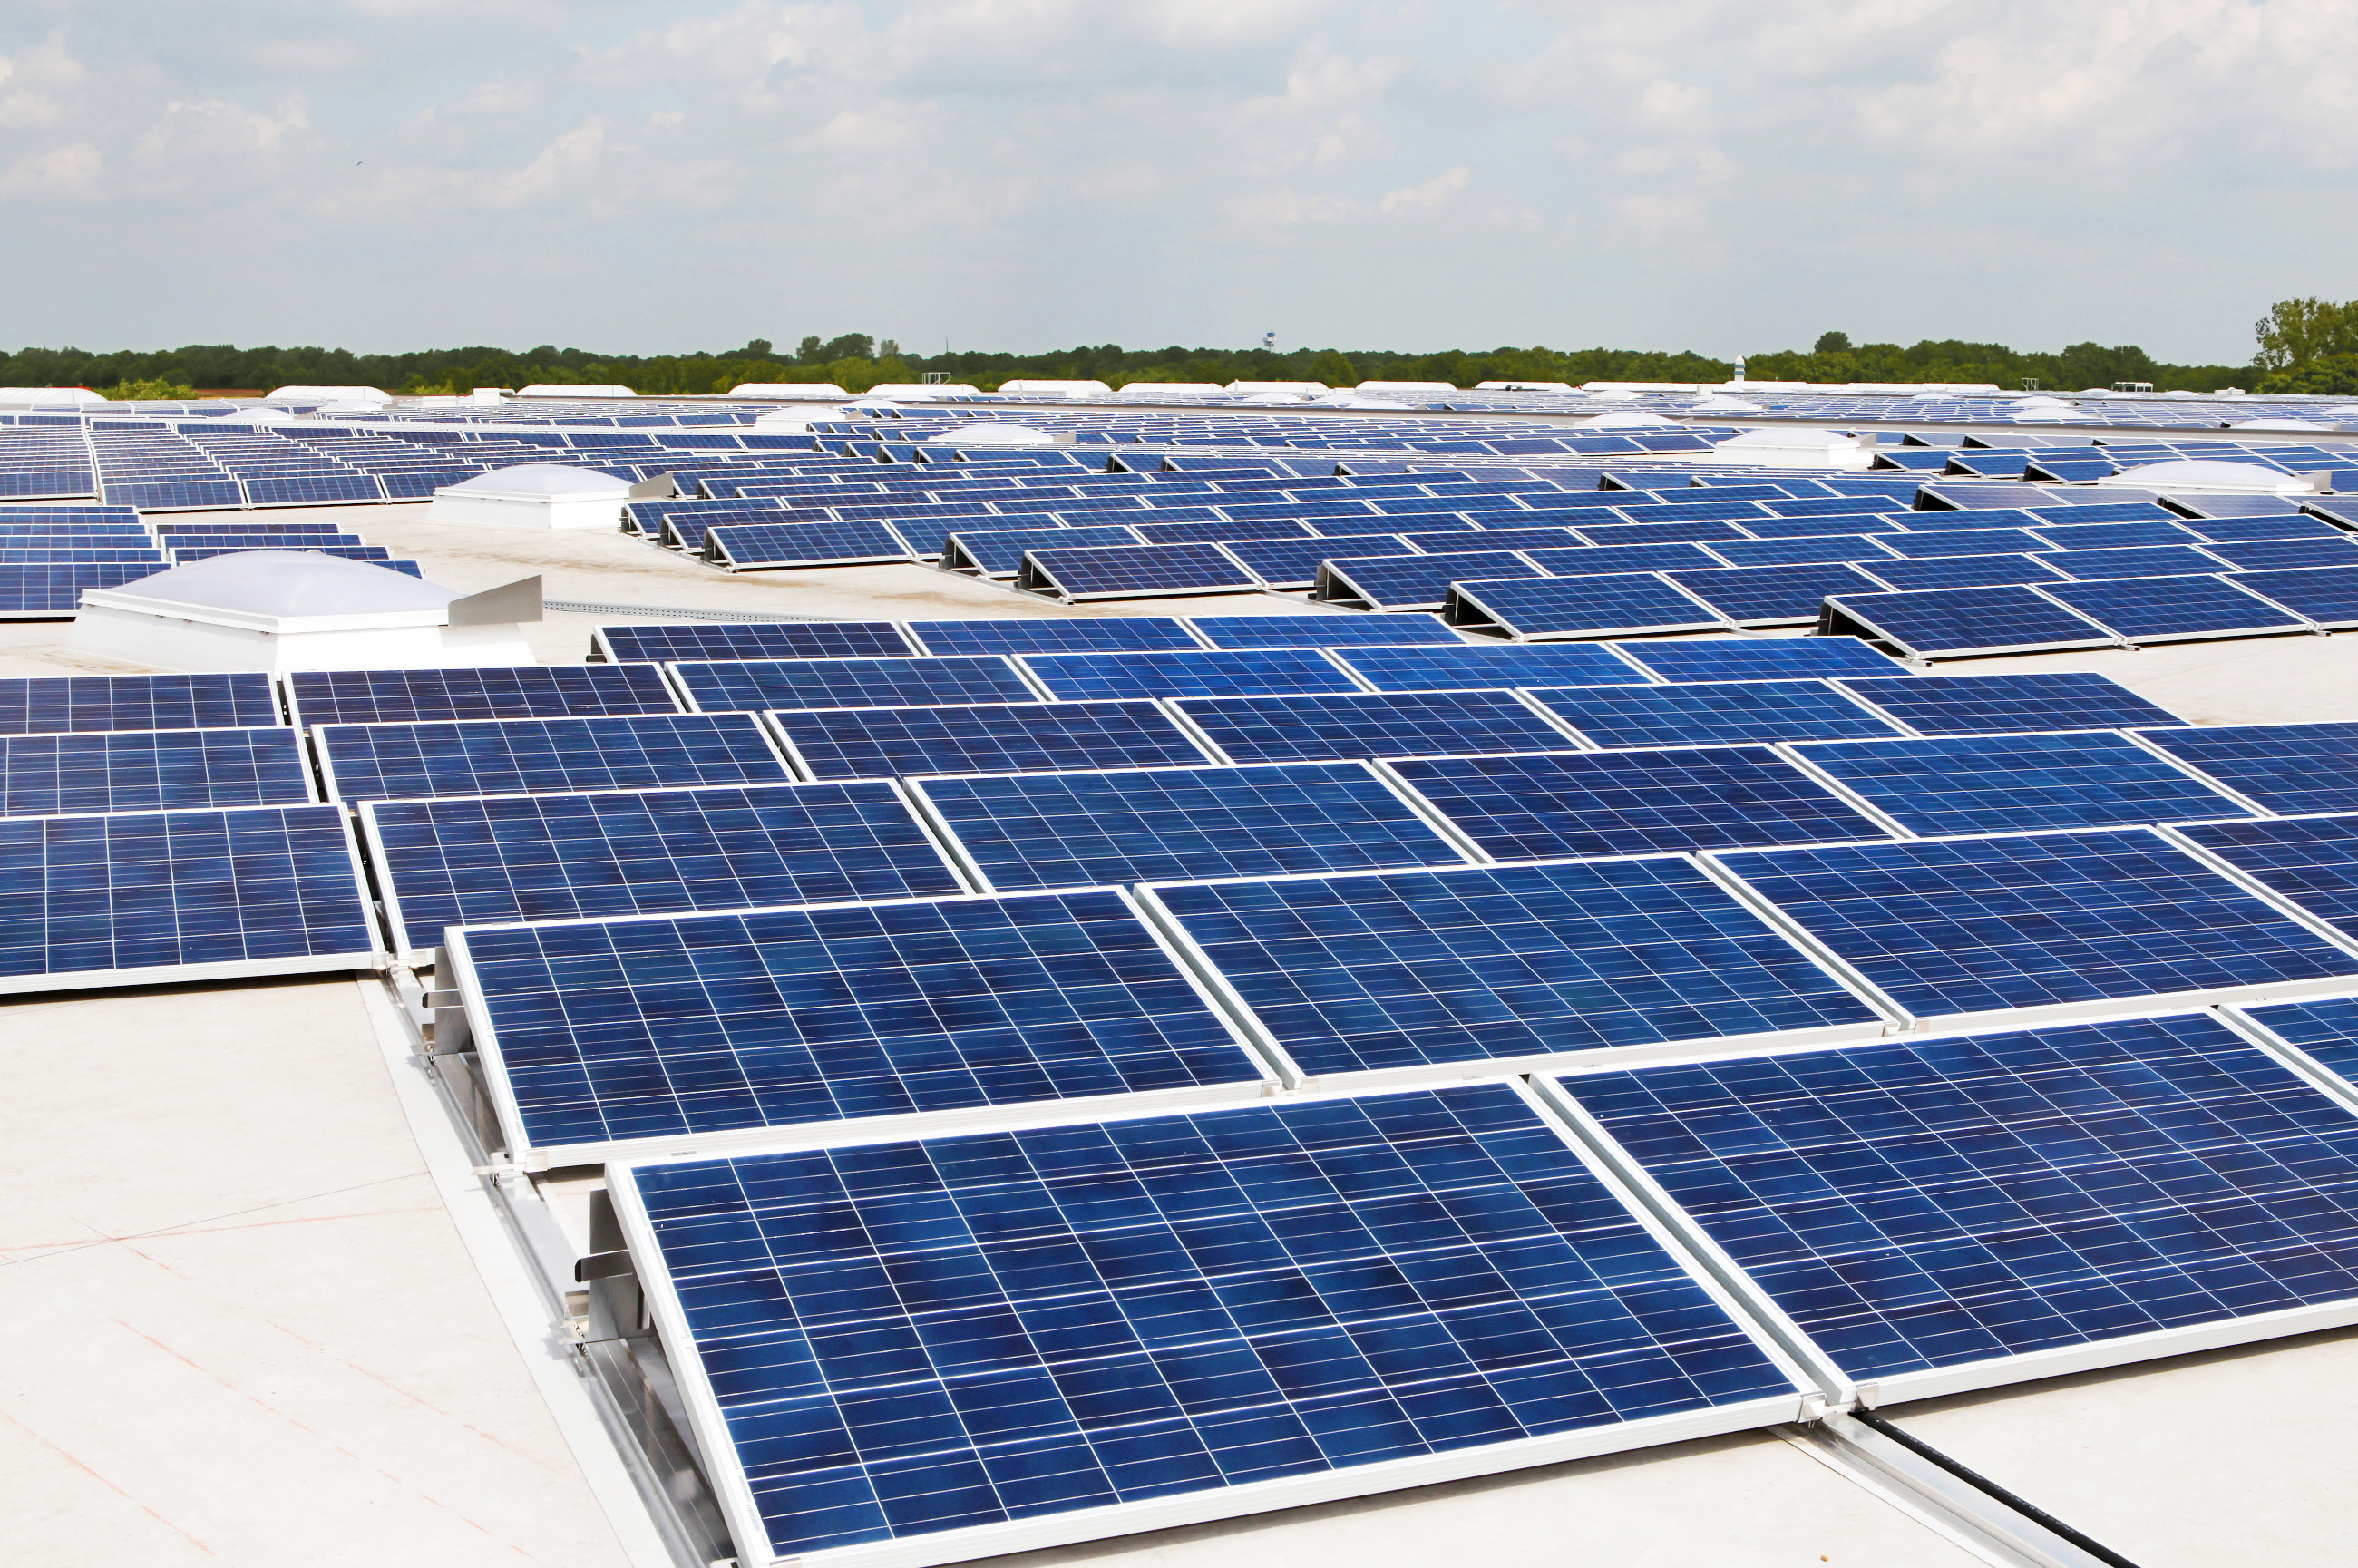
\includegraphics[width=\paperwidth,height=\paperheight]{images/titlepage/titlepic.jpg}%
        };
        %\node[
        %    fill=white,
        %    fill opacity=0.5,
        %    inner sep=0pt,
        %    anchor=west
        %] at (-38.5mm,-105mm) {%
        %    %% Creator: Matplotlib, PGF backend
%%
%% To include the figure in your LaTeX document, write
%%   \input{<filename>.pgf}
%%
%% Make sure the required packages are loaded in your preamble
%%   \usepackage{pgf}
%%
%% Figures using additional raster images can only be included by \input if
%% they are in the same directory as the main LaTeX file. For loading figures
%% from other directories you can use the `import` package
%%   \usepackage{import}
%% and then include the figures with
%%   \import{<path to file>}{<filename>.pgf}
%%
%% Matplotlib used the following preamble
%%   \usepackage{fontspec}
%%   \setmainfont{Bitstream Vera Serif}
%%   \setsansfont{Bitstream Vera Sans}
%%   \setmonofont{Bitstream Vera Sans Mono}
%%
\begingroup%
\makeatletter%
\begin{pgfpicture}%
\pgfpathrectangle{\pgfpointorigin}{\pgfqpoint{8.267700in}{2.000000in}}%
\pgfusepath{use as bounding box, clip}%
\begin{pgfscope}%
\pgfsetbuttcap%
\pgfsetmiterjoin%
\pgfsetlinewidth{0.000000pt}%
\definecolor{currentstroke}{rgb}{0.000000,0.000000,0.000000}%
\pgfsetstrokecolor{currentstroke}%
\pgfsetstrokeopacity{0.000000}%
\pgfsetdash{}{0pt}%
\pgfpathmoveto{\pgfqpoint{0.000000in}{0.000000in}}%
\pgfpathlineto{\pgfqpoint{8.267700in}{0.000000in}}%
\pgfpathlineto{\pgfqpoint{8.267700in}{2.000000in}}%
\pgfpathlineto{\pgfqpoint{0.000000in}{2.000000in}}%
\pgfpathclose%
\pgfusepath{}%
\end{pgfscope}%
\begin{pgfscope}%
\pgfsetbuttcap%
\pgfsetmiterjoin%
\pgfsetlinewidth{0.000000pt}%
\definecolor{currentstroke}{rgb}{0.000000,0.000000,0.000000}%
\pgfsetstrokecolor{currentstroke}%
\pgfsetstrokeopacity{0.000000}%
\pgfsetdash{}{0pt}%
\pgfpathmoveto{\pgfqpoint{0.826770in}{0.100000in}}%
\pgfpathlineto{\pgfqpoint{7.440930in}{0.100000in}}%
\pgfpathlineto{\pgfqpoint{7.440930in}{1.900000in}}%
\pgfpathlineto{\pgfqpoint{0.826770in}{1.900000in}}%
\pgfpathclose%
\pgfusepath{}%
\end{pgfscope}%
\begin{pgfscope}%
\pgfpathrectangle{\pgfqpoint{0.826770in}{0.100000in}}{\pgfqpoint{6.614160in}{1.800000in}} %
\pgfusepath{clip}%
\pgfsetroundcap%
\pgfsetroundjoin%
\pgfsetlinewidth{6.022500pt}%
\definecolor{currentstroke}{rgb}{0.500000,0.000000,0.000000}%
\pgfsetstrokecolor{currentstroke}%
\pgfsetdash{}{0pt}%
\pgfpathmoveto{\pgfqpoint{1.299210in}{1.000000in}}%
\pgfpathlineto{\pgfqpoint{1.333260in}{1.059662in}}%
\pgfpathlineto{\pgfqpoint{1.352176in}{1.088308in}}%
\pgfpathlineto{\pgfqpoint{1.367309in}{1.107297in}}%
\pgfpathlineto{\pgfqpoint{1.380551in}{1.120382in}}%
\pgfpathlineto{\pgfqpoint{1.391901in}{1.128645in}}%
\pgfpathlineto{\pgfqpoint{1.403251in}{1.133983in}}%
\pgfpathlineto{\pgfqpoint{1.412709in}{1.136107in}}%
\pgfpathlineto{\pgfqpoint{1.422167in}{1.136080in}}%
\pgfpathlineto{\pgfqpoint{1.431626in}{1.133903in}}%
\pgfpathlineto{\pgfqpoint{1.441084in}{1.129610in}}%
\pgfpathlineto{\pgfqpoint{1.452434in}{1.121763in}}%
\pgfpathlineto{\pgfqpoint{1.463784in}{1.111146in}}%
\pgfpathlineto{\pgfqpoint{1.477025in}{1.095586in}}%
\pgfpathlineto{\pgfqpoint{1.492158in}{1.074215in}}%
\pgfpathlineto{\pgfqpoint{1.511075in}{1.043401in}}%
\pgfpathlineto{\pgfqpoint{1.545125in}{0.982467in}}%
\pgfpathlineto{\pgfqpoint{1.571608in}{0.936892in}}%
\pgfpathlineto{\pgfqpoint{1.588633in}{0.911366in}}%
\pgfpathlineto{\pgfqpoint{1.603766in}{0.892438in}}%
\pgfpathlineto{\pgfqpoint{1.617007in}{0.879417in}}%
\pgfpathlineto{\pgfqpoint{1.628357in}{0.871213in}}%
\pgfpathlineto{\pgfqpoint{1.639707in}{0.865937in}}%
\pgfpathlineto{\pgfqpoint{1.649166in}{0.863867in}}%
\pgfpathlineto{\pgfqpoint{1.658624in}{0.863948in}}%
\pgfpathlineto{\pgfqpoint{1.668082in}{0.866179in}}%
\pgfpathlineto{\pgfqpoint{1.677540in}{0.870524in}}%
\pgfpathlineto{\pgfqpoint{1.688890in}{0.878431in}}%
\pgfpathlineto{\pgfqpoint{1.700240in}{0.889103in}}%
\pgfpathlineto{\pgfqpoint{1.713482in}{0.904720in}}%
\pgfpathlineto{\pgfqpoint{1.728615in}{0.926145in}}%
\pgfpathlineto{\pgfqpoint{1.747531in}{0.957006in}}%
\pgfpathlineto{\pgfqpoint{1.781581in}{1.017958in}}%
\pgfpathlineto{\pgfqpoint{1.808064in}{1.063488in}}%
\pgfpathlineto{\pgfqpoint{1.825089in}{1.088960in}}%
\pgfpathlineto{\pgfqpoint{1.840222in}{1.107825in}}%
\pgfpathlineto{\pgfqpoint{1.853464in}{1.120782in}}%
\pgfpathlineto{\pgfqpoint{1.864814in}{1.128927in}}%
\pgfpathlineto{\pgfqpoint{1.876164in}{1.134140in}}%
\pgfpathlineto{\pgfqpoint{1.885622in}{1.136157in}}%
\pgfpathlineto{\pgfqpoint{1.895080in}{1.136022in}}%
\pgfpathlineto{\pgfqpoint{1.904539in}{1.133738in}}%
\pgfpathlineto{\pgfqpoint{1.913997in}{1.129341in}}%
\pgfpathlineto{\pgfqpoint{1.925347in}{1.121374in}}%
\pgfpathlineto{\pgfqpoint{1.936697in}{1.110647in}}%
\pgfpathlineto{\pgfqpoint{1.949938in}{1.094973in}}%
\pgfpathlineto{\pgfqpoint{1.965071in}{1.073494in}}%
\pgfpathlineto{\pgfqpoint{1.983988in}{1.042587in}}%
\pgfpathlineto{\pgfqpoint{2.019929in}{0.978223in}}%
\pgfpathlineto{\pgfqpoint{2.046412in}{0.933122in}}%
\pgfpathlineto{\pgfqpoint{2.063437in}{0.908151in}}%
\pgfpathlineto{\pgfqpoint{2.078570in}{0.889856in}}%
\pgfpathlineto{\pgfqpoint{2.091812in}{0.877475in}}%
\pgfpathlineto{\pgfqpoint{2.103162in}{0.869867in}}%
\pgfpathlineto{\pgfqpoint{2.112620in}{0.865783in}}%
\pgfpathlineto{\pgfqpoint{2.122078in}{0.863820in}}%
\pgfpathlineto{\pgfqpoint{2.131537in}{0.864009in}}%
\pgfpathlineto{\pgfqpoint{2.140995in}{0.866346in}}%
\pgfpathlineto{\pgfqpoint{2.150453in}{0.870796in}}%
\pgfpathlineto{\pgfqpoint{2.161803in}{0.878822in}}%
\pgfpathlineto{\pgfqpoint{2.173153in}{0.889604in}}%
\pgfpathlineto{\pgfqpoint{2.186395in}{0.905336in}}%
\pgfpathlineto{\pgfqpoint{2.201528in}{0.926868in}}%
\pgfpathlineto{\pgfqpoint{2.220444in}{0.957821in}}%
\pgfpathlineto{\pgfqpoint{2.256386in}{1.022200in}}%
\pgfpathlineto{\pgfqpoint{2.282869in}{1.067251in}}%
\pgfpathlineto{\pgfqpoint{2.299894in}{1.092165in}}%
\pgfpathlineto{\pgfqpoint{2.315027in}{1.110396in}}%
\pgfpathlineto{\pgfqpoint{2.328268in}{1.122713in}}%
\pgfpathlineto{\pgfqpoint{2.339618in}{1.130260in}}%
\pgfpathlineto{\pgfqpoint{2.349077in}{1.134292in}}%
\pgfpathlineto{\pgfqpoint{2.358535in}{1.136202in}}%
\pgfpathlineto{\pgfqpoint{2.367993in}{1.135959in}}%
\pgfpathlineto{\pgfqpoint{2.377451in}{1.133568in}}%
\pgfpathlineto{\pgfqpoint{2.386910in}{1.129066in}}%
\pgfpathlineto{\pgfqpoint{2.398260in}{1.120981in}}%
\pgfpathlineto{\pgfqpoint{2.409610in}{1.110144in}}%
\pgfpathlineto{\pgfqpoint{2.422851in}{1.094355in}}%
\pgfpathlineto{\pgfqpoint{2.437984in}{1.072770in}}%
\pgfpathlineto{\pgfqpoint{2.456901in}{1.041771in}}%
\pgfpathlineto{\pgfqpoint{2.494734in}{0.974002in}}%
\pgfpathlineto{\pgfqpoint{2.519325in}{0.932376in}}%
\pgfpathlineto{\pgfqpoint{2.536350in}{0.907519in}}%
\pgfpathlineto{\pgfqpoint{2.551483in}{0.889353in}}%
\pgfpathlineto{\pgfqpoint{2.564725in}{0.877101in}}%
\pgfpathlineto{\pgfqpoint{2.576075in}{0.869614in}}%
\pgfpathlineto{\pgfqpoint{2.585533in}{0.865634in}}%
\pgfpathlineto{\pgfqpoint{2.594991in}{0.863778in}}%
\pgfpathlineto{\pgfqpoint{2.604450in}{0.864075in}}%
\pgfpathlineto{\pgfqpoint{2.613908in}{0.866519in}}%
\pgfpathlineto{\pgfqpoint{2.623366in}{0.871073in}}%
\pgfpathlineto{\pgfqpoint{2.634716in}{0.879218in}}%
\pgfpathlineto{\pgfqpoint{2.646066in}{0.890110in}}%
\pgfpathlineto{\pgfqpoint{2.659308in}{0.905955in}}%
\pgfpathlineto{\pgfqpoint{2.674441in}{0.927593in}}%
\pgfpathlineto{\pgfqpoint{2.693357in}{0.958637in}}%
\pgfpathlineto{\pgfqpoint{2.733082in}{1.029776in}}%
\pgfpathlineto{\pgfqpoint{2.757673in}{1.070948in}}%
\pgfpathlineto{\pgfqpoint{2.774698in}{1.095280in}}%
\pgfpathlineto{\pgfqpoint{2.787940in}{1.110897in}}%
\pgfpathlineto{\pgfqpoint{2.801181in}{1.123084in}}%
\pgfpathlineto{\pgfqpoint{2.812531in}{1.130511in}}%
\pgfpathlineto{\pgfqpoint{2.821990in}{1.134438in}}%
\pgfpathlineto{\pgfqpoint{2.831448in}{1.136241in}}%
\pgfpathlineto{\pgfqpoint{2.840906in}{1.135890in}}%
\pgfpathlineto{\pgfqpoint{2.850364in}{1.133393in}}%
\pgfpathlineto{\pgfqpoint{2.859823in}{1.128787in}}%
\pgfpathlineto{\pgfqpoint{2.871173in}{1.120583in}}%
\pgfpathlineto{\pgfqpoint{2.882522in}{1.109636in}}%
\pgfpathlineto{\pgfqpoint{2.895764in}{1.093734in}}%
\pgfpathlineto{\pgfqpoint{2.910897in}{1.072043in}}%
\pgfpathlineto{\pgfqpoint{2.929814in}{1.040954in}}%
\pgfpathlineto{\pgfqpoint{2.971430in}{0.966470in}}%
\pgfpathlineto{\pgfqpoint{2.994130in}{0.928686in}}%
\pgfpathlineto{\pgfqpoint{3.011155in}{0.904414in}}%
\pgfpathlineto{\pgfqpoint{3.024396in}{0.888854in}}%
\pgfpathlineto{\pgfqpoint{3.037638in}{0.876732in}}%
\pgfpathlineto{\pgfqpoint{3.048988in}{0.869365in}}%
\pgfpathlineto{\pgfqpoint{3.058446in}{0.865491in}}%
\pgfpathlineto{\pgfqpoint{3.067904in}{0.863742in}}%
\pgfpathlineto{\pgfqpoint{3.077363in}{0.864146in}}%
\pgfpathlineto{\pgfqpoint{3.086821in}{0.866697in}}%
\pgfpathlineto{\pgfqpoint{3.096279in}{0.871355in}}%
\pgfpathlineto{\pgfqpoint{3.107629in}{0.879618in}}%
\pgfpathlineto{\pgfqpoint{3.118979in}{0.890620in}}%
\pgfpathlineto{\pgfqpoint{3.132220in}{0.906578in}}%
\pgfpathlineto{\pgfqpoint{3.147354in}{0.928321in}}%
\pgfpathlineto{\pgfqpoint{3.166270in}{0.959455in}}%
\pgfpathlineto{\pgfqpoint{3.188970in}{1.000000in}}%
\pgfpathlineto{\pgfqpoint{3.188970in}{1.000000in}}%
\pgfusepath{stroke}%
\end{pgfscope}%
\begin{pgfscope}%
\pgfpathrectangle{\pgfqpoint{0.826770in}{0.100000in}}{\pgfqpoint{6.614160in}{1.800000in}} %
\pgfusepath{clip}%
\pgfsetroundcap%
\pgfsetroundjoin%
\pgfsetlinewidth{6.022500pt}%
\definecolor{currentstroke}{rgb}{0.500000,0.000000,0.000000}%
\pgfsetstrokecolor{currentstroke}%
\pgfsetdash{}{0pt}%
\pgfpathmoveto{\pgfqpoint{3.188970in}{1.000000in}}%
\pgfpathlineto{\pgfqpoint{3.221128in}{1.339353in}}%
\pgfpathlineto{\pgfqpoint{3.238153in}{1.497822in}}%
\pgfpathlineto{\pgfqpoint{3.251395in}{1.603878in}}%
\pgfpathlineto{\pgfqpoint{3.262744in}{1.680025in}}%
\pgfpathlineto{\pgfqpoint{3.272203in}{1.731730in}}%
\pgfpathlineto{\pgfqpoint{3.281661in}{1.771873in}}%
\pgfpathlineto{\pgfqpoint{3.289228in}{1.795229in}}%
\pgfpathlineto{\pgfqpoint{3.294902in}{1.807475in}}%
\pgfpathlineto{\pgfqpoint{3.300577in}{1.815124in}}%
\pgfpathlineto{\pgfqpoint{3.304361in}{1.817647in}}%
\pgfpathlineto{\pgfqpoint{3.308144in}{1.818100in}}%
\pgfpathlineto{\pgfqpoint{3.311927in}{1.816482in}}%
\pgfpathlineto{\pgfqpoint{3.315711in}{1.812798in}}%
\pgfpathlineto{\pgfqpoint{3.321386in}{1.803418in}}%
\pgfpathlineto{\pgfqpoint{3.327061in}{1.789464in}}%
\pgfpathlineto{\pgfqpoint{3.334627in}{1.763885in}}%
\pgfpathlineto{\pgfqpoint{3.342194in}{1.730576in}}%
\pgfpathlineto{\pgfqpoint{3.351652in}{1.678591in}}%
\pgfpathlineto{\pgfqpoint{3.363002in}{1.602139in}}%
\pgfpathlineto{\pgfqpoint{3.376244in}{1.495778in}}%
\pgfpathlineto{\pgfqpoint{3.391377in}{1.355658in}}%
\pgfpathlineto{\pgfqpoint{3.412185in}{1.140809in}}%
\pgfpathlineto{\pgfqpoint{3.463259in}{0.603225in}}%
\pgfpathlineto{\pgfqpoint{3.480284in}{0.452721in}}%
\pgfpathlineto{\pgfqpoint{3.493526in}{0.354631in}}%
\pgfpathlineto{\pgfqpoint{3.504876in}{0.286344in}}%
\pgfpathlineto{\pgfqpoint{3.514334in}{0.241781in}}%
\pgfpathlineto{\pgfqpoint{3.521901in}{0.214730in}}%
\pgfpathlineto{\pgfqpoint{3.529467in}{0.195624in}}%
\pgfpathlineto{\pgfqpoint{3.535142in}{0.186629in}}%
\pgfpathlineto{\pgfqpoint{3.540817in}{0.182264in}}%
\pgfpathlineto{\pgfqpoint{3.544601in}{0.181941in}}%
\pgfpathlineto{\pgfqpoint{3.548384in}{0.183688in}}%
\pgfpathlineto{\pgfqpoint{3.552167in}{0.187501in}}%
\pgfpathlineto{\pgfqpoint{3.557842in}{0.197072in}}%
\pgfpathlineto{\pgfqpoint{3.563517in}{0.211215in}}%
\pgfpathlineto{\pgfqpoint{3.571084in}{0.237041in}}%
\pgfpathlineto{\pgfqpoint{3.578650in}{0.270586in}}%
\pgfpathlineto{\pgfqpoint{3.588108in}{0.322850in}}%
\pgfpathlineto{\pgfqpoint{3.599458in}{0.399606in}}%
\pgfpathlineto{\pgfqpoint{3.612700in}{0.506271in}}%
\pgfpathlineto{\pgfqpoint{3.627833in}{0.646661in}}%
\pgfpathlineto{\pgfqpoint{3.648641in}{0.861727in}}%
\pgfpathlineto{\pgfqpoint{3.699716in}{1.399023in}}%
\pgfpathlineto{\pgfqpoint{3.716741in}{1.549189in}}%
\pgfpathlineto{\pgfqpoint{3.729982in}{1.646948in}}%
\pgfpathlineto{\pgfqpoint{3.741332in}{1.714911in}}%
\pgfpathlineto{\pgfqpoint{3.750791in}{1.759182in}}%
\pgfpathlineto{\pgfqpoint{3.758357in}{1.785988in}}%
\pgfpathlineto{\pgfqpoint{3.765924in}{1.804842in}}%
\pgfpathlineto{\pgfqpoint{3.771599in}{1.813646in}}%
\pgfpathlineto{\pgfqpoint{3.777274in}{1.817817in}}%
\pgfpathlineto{\pgfqpoint{3.781057in}{1.818011in}}%
\pgfpathlineto{\pgfqpoint{3.784840in}{1.816135in}}%
\pgfpathlineto{\pgfqpoint{3.788624in}{1.812192in}}%
\pgfpathlineto{\pgfqpoint{3.794299in}{1.802429in}}%
\pgfpathlineto{\pgfqpoint{3.799973in}{1.788097in}}%
\pgfpathlineto{\pgfqpoint{3.807540in}{1.762026in}}%
\pgfpathlineto{\pgfqpoint{3.815107in}{1.728245in}}%
\pgfpathlineto{\pgfqpoint{3.824565in}{1.675703in}}%
\pgfpathlineto{\pgfqpoint{3.835915in}{1.598643in}}%
\pgfpathlineto{\pgfqpoint{3.849156in}{1.491675in}}%
\pgfpathlineto{\pgfqpoint{3.864290in}{1.351017in}}%
\pgfpathlineto{\pgfqpoint{3.885098in}{1.135737in}}%
\pgfpathlineto{\pgfqpoint{3.934281in}{0.616796in}}%
\pgfpathlineto{\pgfqpoint{3.951306in}{0.464293in}}%
\pgfpathlineto{\pgfqpoint{3.964547in}{0.364234in}}%
\pgfpathlineto{\pgfqpoint{3.975897in}{0.294021in}}%
\pgfpathlineto{\pgfqpoint{3.985355in}{0.247717in}}%
\pgfpathlineto{\pgfqpoint{3.992922in}{0.219204in}}%
\pgfpathlineto{\pgfqpoint{4.000489in}{0.198591in}}%
\pgfpathlineto{\pgfqpoint{4.006164in}{0.188445in}}%
\pgfpathlineto{\pgfqpoint{4.011838in}{0.182919in}}%
\pgfpathlineto{\pgfqpoint{4.015622in}{0.181819in}}%
\pgfpathlineto{\pgfqpoint{4.019405in}{0.182790in}}%
\pgfpathlineto{\pgfqpoint{4.023188in}{0.185829in}}%
\pgfpathlineto{\pgfqpoint{4.028863in}{0.194248in}}%
\pgfpathlineto{\pgfqpoint{4.034538in}{0.207255in}}%
\pgfpathlineto{\pgfqpoint{4.042105in}{0.231602in}}%
\pgfpathlineto{\pgfqpoint{4.049672in}{0.263723in}}%
\pgfpathlineto{\pgfqpoint{4.059130in}{0.314306in}}%
\pgfpathlineto{\pgfqpoint{4.070480in}{0.389225in}}%
\pgfpathlineto{\pgfqpoint{4.083721in}{0.494050in}}%
\pgfpathlineto{\pgfqpoint{4.098854in}{0.632801in}}%
\pgfpathlineto{\pgfqpoint{4.119663in}{0.846536in}}%
\pgfpathlineto{\pgfqpoint{4.172629in}{1.403508in}}%
\pgfpathlineto{\pgfqpoint{4.187762in}{1.537649in}}%
\pgfpathlineto{\pgfqpoint{4.201004in}{1.637382in}}%
\pgfpathlineto{\pgfqpoint{4.212354in}{1.707276in}}%
\pgfpathlineto{\pgfqpoint{4.221812in}{1.753291in}}%
\pgfpathlineto{\pgfqpoint{4.229378in}{1.781561in}}%
\pgfpathlineto{\pgfqpoint{4.236945in}{1.801923in}}%
\pgfpathlineto{\pgfqpoint{4.242620in}{1.811878in}}%
\pgfpathlineto{\pgfqpoint{4.248295in}{1.817210in}}%
\pgfpathlineto{\pgfqpoint{4.252078in}{1.818181in}}%
\pgfpathlineto{\pgfqpoint{4.255862in}{1.817081in}}%
\pgfpathlineto{\pgfqpoint{4.259645in}{1.813912in}}%
\pgfpathlineto{\pgfqpoint{4.265320in}{1.805301in}}%
\pgfpathlineto{\pgfqpoint{4.270995in}{1.792105in}}%
\pgfpathlineto{\pgfqpoint{4.278561in}{1.767511in}}%
\pgfpathlineto{\pgfqpoint{4.286128in}{1.735151in}}%
\pgfpathlineto{\pgfqpoint{4.295586in}{1.684287in}}%
\pgfpathlineto{\pgfqpoint{4.306936in}{1.609059in}}%
\pgfpathlineto{\pgfqpoint{4.320178in}{1.503926in}}%
\pgfpathlineto{\pgfqpoint{4.335311in}{1.364898in}}%
\pgfpathlineto{\pgfqpoint{4.356119in}{1.150936in}}%
\pgfpathlineto{\pgfqpoint{4.409085in}{0.594256in}}%
\pgfpathlineto{\pgfqpoint{4.424219in}{0.460414in}}%
\pgfpathlineto{\pgfqpoint{4.437460in}{0.361008in}}%
\pgfpathlineto{\pgfqpoint{4.448810in}{0.291434in}}%
\pgfpathlineto{\pgfqpoint{4.458268in}{0.245708in}}%
\pgfpathlineto{\pgfqpoint{4.465835in}{0.217682in}}%
\pgfpathlineto{\pgfqpoint{4.473401in}{0.197571in}}%
\pgfpathlineto{\pgfqpoint{4.479076in}{0.187808in}}%
\pgfpathlineto{\pgfqpoint{4.484751in}{0.182669in}}%
\pgfpathlineto{\pgfqpoint{4.488535in}{0.181827in}}%
\pgfpathlineto{\pgfqpoint{4.492318in}{0.183057in}}%
\pgfpathlineto{\pgfqpoint{4.496101in}{0.186354in}}%
\pgfpathlineto{\pgfqpoint{4.501776in}{0.195158in}}%
\pgfpathlineto{\pgfqpoint{4.507451in}{0.208544in}}%
\pgfpathlineto{\pgfqpoint{4.515018in}{0.233384in}}%
\pgfpathlineto{\pgfqpoint{4.522584in}{0.265982in}}%
\pgfpathlineto{\pgfqpoint{4.532043in}{0.317127in}}%
\pgfpathlineto{\pgfqpoint{4.543393in}{0.392662in}}%
\pgfpathlineto{\pgfqpoint{4.556634in}{0.498104in}}%
\pgfpathlineto{\pgfqpoint{4.571767in}{0.637406in}}%
\pgfpathlineto{\pgfqpoint{4.592576in}{0.851594in}}%
\pgfpathlineto{\pgfqpoint{4.645542in}{1.407976in}}%
\pgfpathlineto{\pgfqpoint{4.660675in}{1.541517in}}%
\pgfpathlineto{\pgfqpoint{4.673917in}{1.640596in}}%
\pgfpathlineto{\pgfqpoint{4.685266in}{1.709849in}}%
\pgfpathlineto{\pgfqpoint{4.694725in}{1.755285in}}%
\pgfpathlineto{\pgfqpoint{4.702291in}{1.783068in}}%
\pgfpathlineto{\pgfqpoint{4.709858in}{1.802928in}}%
\pgfpathlineto{\pgfqpoint{4.715533in}{1.812499in}}%
\pgfpathlineto{\pgfqpoint{4.721208in}{1.817445in}}%
\pgfpathlineto{\pgfqpoint{4.724991in}{1.818157in}}%
\pgfpathlineto{\pgfqpoint{4.728774in}{1.816798in}}%
\pgfpathlineto{\pgfqpoint{4.732558in}{1.813371in}}%
\pgfpathlineto{\pgfqpoint{4.738233in}{1.804376in}}%
\pgfpathlineto{\pgfqpoint{4.743908in}{1.790800in}}%
\pgfpathlineto{\pgfqpoint{4.751474in}{1.765713in}}%
\pgfpathlineto{\pgfqpoint{4.759041in}{1.732878in}}%
\pgfpathlineto{\pgfqpoint{4.768499in}{1.681453in}}%
\pgfpathlineto{\pgfqpoint{4.779849in}{1.605611in}}%
\pgfpathlineto{\pgfqpoint{4.793091in}{1.499862in}}%
\pgfpathlineto{\pgfqpoint{4.808224in}{1.360285in}}%
\pgfpathlineto{\pgfqpoint{4.829032in}{1.145875in}}%
\pgfpathlineto{\pgfqpoint{4.880107in}{0.607733in}}%
\pgfpathlineto{\pgfqpoint{4.897131in}{0.456557in}}%
\pgfpathlineto{\pgfqpoint{4.910373in}{0.357807in}}%
\pgfpathlineto{\pgfqpoint{4.921723in}{0.288875in}}%
\pgfpathlineto{\pgfqpoint{4.931181in}{0.243730in}}%
\pgfpathlineto{\pgfqpoint{4.938748in}{0.216190in}}%
\pgfpathlineto{\pgfqpoint{4.946314in}{0.196582in}}%
\pgfpathlineto{\pgfqpoint{4.951989in}{0.187202in}}%
\pgfpathlineto{\pgfqpoint{4.957664in}{0.182450in}}%
\pgfpathlineto{\pgfqpoint{4.961448in}{0.181868in}}%
\pgfpathlineto{\pgfqpoint{4.965231in}{0.183356in}}%
\pgfpathlineto{\pgfqpoint{4.969014in}{0.186911in}}%
\pgfpathlineto{\pgfqpoint{4.974689in}{0.196099in}}%
\pgfpathlineto{\pgfqpoint{4.980364in}{0.209864in}}%
\pgfpathlineto{\pgfqpoint{4.987931in}{0.235197in}}%
\pgfpathlineto{\pgfqpoint{4.995497in}{0.268270in}}%
\pgfpathlineto{\pgfqpoint{5.004956in}{0.319975in}}%
\pgfpathlineto{\pgfqpoint{5.016305in}{0.396122in}}%
\pgfpathlineto{\pgfqpoint{5.029547in}{0.502178in}}%
\pgfpathlineto{\pgfqpoint{5.044680in}{0.642027in}}%
\pgfpathlineto{\pgfqpoint{5.065488in}{0.856657in}}%
\pgfpathlineto{\pgfqpoint{5.078730in}{1.000000in}}%
\pgfpathlineto{\pgfqpoint{5.078730in}{1.000000in}}%
\pgfusepath{stroke}%
\end{pgfscope}%
\begin{pgfscope}%
\pgfpathrectangle{\pgfqpoint{0.826770in}{0.100000in}}{\pgfqpoint{6.614160in}{1.800000in}} %
\pgfusepath{clip}%
\pgfsetroundcap%
\pgfsetroundjoin%
\pgfsetlinewidth{6.022500pt}%
\definecolor{currentstroke}{rgb}{0.500000,0.000000,0.000000}%
\pgfsetstrokecolor{currentstroke}%
\pgfsetdash{}{0pt}%
\pgfpathmoveto{\pgfqpoint{5.078730in}{1.000000in}}%
\pgfpathlineto{\pgfqpoint{5.112780in}{1.059662in}}%
\pgfpathlineto{\pgfqpoint{5.131696in}{1.088308in}}%
\pgfpathlineto{\pgfqpoint{5.146829in}{1.107297in}}%
\pgfpathlineto{\pgfqpoint{5.160071in}{1.120382in}}%
\pgfpathlineto{\pgfqpoint{5.171421in}{1.128645in}}%
\pgfpathlineto{\pgfqpoint{5.182771in}{1.133983in}}%
\pgfpathlineto{\pgfqpoint{5.192229in}{1.136107in}}%
\pgfpathlineto{\pgfqpoint{5.201687in}{1.136080in}}%
\pgfpathlineto{\pgfqpoint{5.211146in}{1.133903in}}%
\pgfpathlineto{\pgfqpoint{5.220604in}{1.129610in}}%
\pgfpathlineto{\pgfqpoint{5.231954in}{1.121763in}}%
\pgfpathlineto{\pgfqpoint{5.243304in}{1.111146in}}%
\pgfpathlineto{\pgfqpoint{5.256545in}{1.095586in}}%
\pgfpathlineto{\pgfqpoint{5.271678in}{1.074215in}}%
\pgfpathlineto{\pgfqpoint{5.290595in}{1.043401in}}%
\pgfpathlineto{\pgfqpoint{5.324645in}{0.982467in}}%
\pgfpathlineto{\pgfqpoint{5.351128in}{0.936892in}}%
\pgfpathlineto{\pgfqpoint{5.368153in}{0.911366in}}%
\pgfpathlineto{\pgfqpoint{5.383286in}{0.892438in}}%
\pgfpathlineto{\pgfqpoint{5.396527in}{0.879417in}}%
\pgfpathlineto{\pgfqpoint{5.407877in}{0.871213in}}%
\pgfpathlineto{\pgfqpoint{5.419227in}{0.865937in}}%
\pgfpathlineto{\pgfqpoint{5.428686in}{0.863867in}}%
\pgfpathlineto{\pgfqpoint{5.438144in}{0.863948in}}%
\pgfpathlineto{\pgfqpoint{5.447602in}{0.866179in}}%
\pgfpathlineto{\pgfqpoint{5.457060in}{0.870524in}}%
\pgfpathlineto{\pgfqpoint{5.468410in}{0.878431in}}%
\pgfpathlineto{\pgfqpoint{5.479760in}{0.889103in}}%
\pgfpathlineto{\pgfqpoint{5.493002in}{0.904720in}}%
\pgfpathlineto{\pgfqpoint{5.508135in}{0.926145in}}%
\pgfpathlineto{\pgfqpoint{5.527051in}{0.957006in}}%
\pgfpathlineto{\pgfqpoint{5.561101in}{1.017958in}}%
\pgfpathlineto{\pgfqpoint{5.587584in}{1.063488in}}%
\pgfpathlineto{\pgfqpoint{5.604609in}{1.088960in}}%
\pgfpathlineto{\pgfqpoint{5.619742in}{1.107825in}}%
\pgfpathlineto{\pgfqpoint{5.632984in}{1.120782in}}%
\pgfpathlineto{\pgfqpoint{5.644334in}{1.128927in}}%
\pgfpathlineto{\pgfqpoint{5.655684in}{1.134140in}}%
\pgfpathlineto{\pgfqpoint{5.665142in}{1.136157in}}%
\pgfpathlineto{\pgfqpoint{5.674600in}{1.136022in}}%
\pgfpathlineto{\pgfqpoint{5.684059in}{1.133738in}}%
\pgfpathlineto{\pgfqpoint{5.693517in}{1.129341in}}%
\pgfpathlineto{\pgfqpoint{5.704867in}{1.121374in}}%
\pgfpathlineto{\pgfqpoint{5.716217in}{1.110647in}}%
\pgfpathlineto{\pgfqpoint{5.729458in}{1.094973in}}%
\pgfpathlineto{\pgfqpoint{5.744591in}{1.073494in}}%
\pgfpathlineto{\pgfqpoint{5.763508in}{1.042587in}}%
\pgfpathlineto{\pgfqpoint{5.799449in}{0.978223in}}%
\pgfpathlineto{\pgfqpoint{5.825932in}{0.933122in}}%
\pgfpathlineto{\pgfqpoint{5.842957in}{0.908151in}}%
\pgfpathlineto{\pgfqpoint{5.858090in}{0.889856in}}%
\pgfpathlineto{\pgfqpoint{5.871332in}{0.877475in}}%
\pgfpathlineto{\pgfqpoint{5.882682in}{0.869867in}}%
\pgfpathlineto{\pgfqpoint{5.892140in}{0.865783in}}%
\pgfpathlineto{\pgfqpoint{5.901598in}{0.863820in}}%
\pgfpathlineto{\pgfqpoint{5.911057in}{0.864009in}}%
\pgfpathlineto{\pgfqpoint{5.920515in}{0.866346in}}%
\pgfpathlineto{\pgfqpoint{5.929973in}{0.870796in}}%
\pgfpathlineto{\pgfqpoint{5.941323in}{0.878822in}}%
\pgfpathlineto{\pgfqpoint{5.952673in}{0.889604in}}%
\pgfpathlineto{\pgfqpoint{5.965915in}{0.905336in}}%
\pgfpathlineto{\pgfqpoint{5.981048in}{0.926868in}}%
\pgfpathlineto{\pgfqpoint{5.999964in}{0.957821in}}%
\pgfpathlineto{\pgfqpoint{6.035906in}{1.022200in}}%
\pgfpathlineto{\pgfqpoint{6.062389in}{1.067251in}}%
\pgfpathlineto{\pgfqpoint{6.079414in}{1.092165in}}%
\pgfpathlineto{\pgfqpoint{6.094547in}{1.110396in}}%
\pgfpathlineto{\pgfqpoint{6.107788in}{1.122713in}}%
\pgfpathlineto{\pgfqpoint{6.119138in}{1.130260in}}%
\pgfpathlineto{\pgfqpoint{6.128597in}{1.134292in}}%
\pgfpathlineto{\pgfqpoint{6.138055in}{1.136202in}}%
\pgfpathlineto{\pgfqpoint{6.147513in}{1.135959in}}%
\pgfpathlineto{\pgfqpoint{6.156971in}{1.133568in}}%
\pgfpathlineto{\pgfqpoint{6.166430in}{1.129066in}}%
\pgfpathlineto{\pgfqpoint{6.177780in}{1.120981in}}%
\pgfpathlineto{\pgfqpoint{6.189130in}{1.110144in}}%
\pgfpathlineto{\pgfqpoint{6.202371in}{1.094355in}}%
\pgfpathlineto{\pgfqpoint{6.217504in}{1.072770in}}%
\pgfpathlineto{\pgfqpoint{6.236421in}{1.041771in}}%
\pgfpathlineto{\pgfqpoint{6.274254in}{0.974002in}}%
\pgfpathlineto{\pgfqpoint{6.298845in}{0.932376in}}%
\pgfpathlineto{\pgfqpoint{6.315870in}{0.907519in}}%
\pgfpathlineto{\pgfqpoint{6.331003in}{0.889353in}}%
\pgfpathlineto{\pgfqpoint{6.344245in}{0.877101in}}%
\pgfpathlineto{\pgfqpoint{6.355595in}{0.869614in}}%
\pgfpathlineto{\pgfqpoint{6.365053in}{0.865634in}}%
\pgfpathlineto{\pgfqpoint{6.374511in}{0.863778in}}%
\pgfpathlineto{\pgfqpoint{6.383970in}{0.864075in}}%
\pgfpathlineto{\pgfqpoint{6.393428in}{0.866519in}}%
\pgfpathlineto{\pgfqpoint{6.402886in}{0.871073in}}%
\pgfpathlineto{\pgfqpoint{6.414236in}{0.879218in}}%
\pgfpathlineto{\pgfqpoint{6.425586in}{0.890110in}}%
\pgfpathlineto{\pgfqpoint{6.438828in}{0.905955in}}%
\pgfpathlineto{\pgfqpoint{6.453961in}{0.927593in}}%
\pgfpathlineto{\pgfqpoint{6.472877in}{0.958637in}}%
\pgfpathlineto{\pgfqpoint{6.512602in}{1.029776in}}%
\pgfpathlineto{\pgfqpoint{6.537193in}{1.070948in}}%
\pgfpathlineto{\pgfqpoint{6.554218in}{1.095280in}}%
\pgfpathlineto{\pgfqpoint{6.567460in}{1.110897in}}%
\pgfpathlineto{\pgfqpoint{6.580701in}{1.123084in}}%
\pgfpathlineto{\pgfqpoint{6.592051in}{1.130511in}}%
\pgfpathlineto{\pgfqpoint{6.601510in}{1.134438in}}%
\pgfpathlineto{\pgfqpoint{6.610968in}{1.136241in}}%
\pgfpathlineto{\pgfqpoint{6.620426in}{1.135890in}}%
\pgfpathlineto{\pgfqpoint{6.629884in}{1.133393in}}%
\pgfpathlineto{\pgfqpoint{6.639343in}{1.128787in}}%
\pgfpathlineto{\pgfqpoint{6.650693in}{1.120583in}}%
\pgfpathlineto{\pgfqpoint{6.662042in}{1.109636in}}%
\pgfpathlineto{\pgfqpoint{6.675284in}{1.093734in}}%
\pgfpathlineto{\pgfqpoint{6.690417in}{1.072043in}}%
\pgfpathlineto{\pgfqpoint{6.709334in}{1.040954in}}%
\pgfpathlineto{\pgfqpoint{6.750950in}{0.966470in}}%
\pgfpathlineto{\pgfqpoint{6.773650in}{0.928686in}}%
\pgfpathlineto{\pgfqpoint{6.790675in}{0.904414in}}%
\pgfpathlineto{\pgfqpoint{6.803916in}{0.888854in}}%
\pgfpathlineto{\pgfqpoint{6.817158in}{0.876732in}}%
\pgfpathlineto{\pgfqpoint{6.828508in}{0.869365in}}%
\pgfpathlineto{\pgfqpoint{6.837966in}{0.865491in}}%
\pgfpathlineto{\pgfqpoint{6.847424in}{0.863742in}}%
\pgfpathlineto{\pgfqpoint{6.856883in}{0.864146in}}%
\pgfpathlineto{\pgfqpoint{6.866341in}{0.866697in}}%
\pgfpathlineto{\pgfqpoint{6.875799in}{0.871355in}}%
\pgfpathlineto{\pgfqpoint{6.887149in}{0.879618in}}%
\pgfpathlineto{\pgfqpoint{6.898499in}{0.890620in}}%
\pgfpathlineto{\pgfqpoint{6.911740in}{0.906578in}}%
\pgfpathlineto{\pgfqpoint{6.926874in}{0.928321in}}%
\pgfpathlineto{\pgfqpoint{6.945790in}{0.959455in}}%
\pgfpathlineto{\pgfqpoint{6.968490in}{1.000000in}}%
\pgfpathlineto{\pgfqpoint{6.968490in}{1.000000in}}%
\pgfusepath{stroke}%
\end{pgfscope}%
\begin{pgfscope}%
\pgfpathrectangle{\pgfqpoint{0.826770in}{0.100000in}}{\pgfqpoint{6.614160in}{1.800000in}} %
\pgfusepath{clip}%
\pgfsetroundcap%
\pgfsetroundjoin%
\pgfsetlinewidth{4.015000pt}%
\definecolor{currentstroke}{rgb}{0.750000,0.000000,0.000000}%
\pgfsetstrokecolor{currentstroke}%
\pgfsetdash{}{0pt}%
\pgfpathmoveto{\pgfqpoint{1.299210in}{1.000000in}}%
\pgfpathlineto{\pgfqpoint{1.333260in}{1.059662in}}%
\pgfpathlineto{\pgfqpoint{1.352176in}{1.088308in}}%
\pgfpathlineto{\pgfqpoint{1.367309in}{1.107297in}}%
\pgfpathlineto{\pgfqpoint{1.380551in}{1.120382in}}%
\pgfpathlineto{\pgfqpoint{1.391901in}{1.128645in}}%
\pgfpathlineto{\pgfqpoint{1.403251in}{1.133983in}}%
\pgfpathlineto{\pgfqpoint{1.412709in}{1.136107in}}%
\pgfpathlineto{\pgfqpoint{1.422167in}{1.136080in}}%
\pgfpathlineto{\pgfqpoint{1.431626in}{1.133903in}}%
\pgfpathlineto{\pgfqpoint{1.441084in}{1.129610in}}%
\pgfpathlineto{\pgfqpoint{1.452434in}{1.121763in}}%
\pgfpathlineto{\pgfqpoint{1.463784in}{1.111146in}}%
\pgfpathlineto{\pgfqpoint{1.477025in}{1.095586in}}%
\pgfpathlineto{\pgfqpoint{1.492158in}{1.074215in}}%
\pgfpathlineto{\pgfqpoint{1.511075in}{1.043401in}}%
\pgfpathlineto{\pgfqpoint{1.545125in}{0.982467in}}%
\pgfpathlineto{\pgfqpoint{1.571608in}{0.936892in}}%
\pgfpathlineto{\pgfqpoint{1.588633in}{0.911366in}}%
\pgfpathlineto{\pgfqpoint{1.603766in}{0.892438in}}%
\pgfpathlineto{\pgfqpoint{1.617007in}{0.879417in}}%
\pgfpathlineto{\pgfqpoint{1.628357in}{0.871213in}}%
\pgfpathlineto{\pgfqpoint{1.639707in}{0.865937in}}%
\pgfpathlineto{\pgfqpoint{1.649166in}{0.863867in}}%
\pgfpathlineto{\pgfqpoint{1.658624in}{0.863948in}}%
\pgfpathlineto{\pgfqpoint{1.668082in}{0.866179in}}%
\pgfpathlineto{\pgfqpoint{1.677540in}{0.870524in}}%
\pgfpathlineto{\pgfqpoint{1.688890in}{0.878431in}}%
\pgfpathlineto{\pgfqpoint{1.700240in}{0.889103in}}%
\pgfpathlineto{\pgfqpoint{1.713482in}{0.904720in}}%
\pgfpathlineto{\pgfqpoint{1.728615in}{0.926145in}}%
\pgfpathlineto{\pgfqpoint{1.747531in}{0.957006in}}%
\pgfpathlineto{\pgfqpoint{1.781581in}{1.017958in}}%
\pgfpathlineto{\pgfqpoint{1.808064in}{1.063488in}}%
\pgfpathlineto{\pgfqpoint{1.825089in}{1.088960in}}%
\pgfpathlineto{\pgfqpoint{1.840222in}{1.107825in}}%
\pgfpathlineto{\pgfqpoint{1.853464in}{1.120782in}}%
\pgfpathlineto{\pgfqpoint{1.864814in}{1.128927in}}%
\pgfpathlineto{\pgfqpoint{1.876164in}{1.134140in}}%
\pgfpathlineto{\pgfqpoint{1.885622in}{1.136157in}}%
\pgfpathlineto{\pgfqpoint{1.895080in}{1.136022in}}%
\pgfpathlineto{\pgfqpoint{1.904539in}{1.133738in}}%
\pgfpathlineto{\pgfqpoint{1.913997in}{1.129341in}}%
\pgfpathlineto{\pgfqpoint{1.925347in}{1.121374in}}%
\pgfpathlineto{\pgfqpoint{1.936697in}{1.110647in}}%
\pgfpathlineto{\pgfqpoint{1.949938in}{1.094973in}}%
\pgfpathlineto{\pgfqpoint{1.965071in}{1.073494in}}%
\pgfpathlineto{\pgfqpoint{1.983988in}{1.042587in}}%
\pgfpathlineto{\pgfqpoint{2.019929in}{0.978223in}}%
\pgfpathlineto{\pgfqpoint{2.046412in}{0.933122in}}%
\pgfpathlineto{\pgfqpoint{2.063437in}{0.908151in}}%
\pgfpathlineto{\pgfqpoint{2.078570in}{0.889856in}}%
\pgfpathlineto{\pgfqpoint{2.091812in}{0.877475in}}%
\pgfpathlineto{\pgfqpoint{2.103162in}{0.869867in}}%
\pgfpathlineto{\pgfqpoint{2.112620in}{0.865783in}}%
\pgfpathlineto{\pgfqpoint{2.122078in}{0.863820in}}%
\pgfpathlineto{\pgfqpoint{2.131537in}{0.864009in}}%
\pgfpathlineto{\pgfqpoint{2.140995in}{0.866346in}}%
\pgfpathlineto{\pgfqpoint{2.150453in}{0.870796in}}%
\pgfpathlineto{\pgfqpoint{2.161803in}{0.878822in}}%
\pgfpathlineto{\pgfqpoint{2.173153in}{0.889604in}}%
\pgfpathlineto{\pgfqpoint{2.186395in}{0.905336in}}%
\pgfpathlineto{\pgfqpoint{2.201528in}{0.926868in}}%
\pgfpathlineto{\pgfqpoint{2.220444in}{0.957821in}}%
\pgfpathlineto{\pgfqpoint{2.256386in}{1.022200in}}%
\pgfpathlineto{\pgfqpoint{2.282869in}{1.067251in}}%
\pgfpathlineto{\pgfqpoint{2.299894in}{1.092165in}}%
\pgfpathlineto{\pgfqpoint{2.315027in}{1.110396in}}%
\pgfpathlineto{\pgfqpoint{2.328268in}{1.122713in}}%
\pgfpathlineto{\pgfqpoint{2.339618in}{1.130260in}}%
\pgfpathlineto{\pgfqpoint{2.349077in}{1.134292in}}%
\pgfpathlineto{\pgfqpoint{2.358535in}{1.136202in}}%
\pgfpathlineto{\pgfqpoint{2.367993in}{1.135959in}}%
\pgfpathlineto{\pgfqpoint{2.377451in}{1.133568in}}%
\pgfpathlineto{\pgfqpoint{2.386910in}{1.129066in}}%
\pgfpathlineto{\pgfqpoint{2.398260in}{1.120981in}}%
\pgfpathlineto{\pgfqpoint{2.409610in}{1.110144in}}%
\pgfpathlineto{\pgfqpoint{2.422851in}{1.094355in}}%
\pgfpathlineto{\pgfqpoint{2.437984in}{1.072770in}}%
\pgfpathlineto{\pgfqpoint{2.456901in}{1.041771in}}%
\pgfpathlineto{\pgfqpoint{2.494734in}{0.974002in}}%
\pgfpathlineto{\pgfqpoint{2.519325in}{0.932376in}}%
\pgfpathlineto{\pgfqpoint{2.536350in}{0.907519in}}%
\pgfpathlineto{\pgfqpoint{2.551483in}{0.889353in}}%
\pgfpathlineto{\pgfqpoint{2.564725in}{0.877101in}}%
\pgfpathlineto{\pgfqpoint{2.576075in}{0.869614in}}%
\pgfpathlineto{\pgfqpoint{2.585533in}{0.865634in}}%
\pgfpathlineto{\pgfqpoint{2.594991in}{0.863778in}}%
\pgfpathlineto{\pgfqpoint{2.604450in}{0.864075in}}%
\pgfpathlineto{\pgfqpoint{2.613908in}{0.866519in}}%
\pgfpathlineto{\pgfqpoint{2.623366in}{0.871073in}}%
\pgfpathlineto{\pgfqpoint{2.634716in}{0.879218in}}%
\pgfpathlineto{\pgfqpoint{2.646066in}{0.890110in}}%
\pgfpathlineto{\pgfqpoint{2.659308in}{0.905955in}}%
\pgfpathlineto{\pgfqpoint{2.674441in}{0.927593in}}%
\pgfpathlineto{\pgfqpoint{2.693357in}{0.958637in}}%
\pgfpathlineto{\pgfqpoint{2.733082in}{1.029776in}}%
\pgfpathlineto{\pgfqpoint{2.757673in}{1.070948in}}%
\pgfpathlineto{\pgfqpoint{2.774698in}{1.095280in}}%
\pgfpathlineto{\pgfqpoint{2.787940in}{1.110897in}}%
\pgfpathlineto{\pgfqpoint{2.801181in}{1.123084in}}%
\pgfpathlineto{\pgfqpoint{2.812531in}{1.130511in}}%
\pgfpathlineto{\pgfqpoint{2.821990in}{1.134438in}}%
\pgfpathlineto{\pgfqpoint{2.831448in}{1.136241in}}%
\pgfpathlineto{\pgfqpoint{2.840906in}{1.135890in}}%
\pgfpathlineto{\pgfqpoint{2.850364in}{1.133393in}}%
\pgfpathlineto{\pgfqpoint{2.859823in}{1.128787in}}%
\pgfpathlineto{\pgfqpoint{2.871173in}{1.120583in}}%
\pgfpathlineto{\pgfqpoint{2.882522in}{1.109636in}}%
\pgfpathlineto{\pgfqpoint{2.895764in}{1.093734in}}%
\pgfpathlineto{\pgfqpoint{2.910897in}{1.072043in}}%
\pgfpathlineto{\pgfqpoint{2.929814in}{1.040954in}}%
\pgfpathlineto{\pgfqpoint{2.971430in}{0.966470in}}%
\pgfpathlineto{\pgfqpoint{2.994130in}{0.928686in}}%
\pgfpathlineto{\pgfqpoint{3.011155in}{0.904414in}}%
\pgfpathlineto{\pgfqpoint{3.024396in}{0.888854in}}%
\pgfpathlineto{\pgfqpoint{3.037638in}{0.876732in}}%
\pgfpathlineto{\pgfqpoint{3.048988in}{0.869365in}}%
\pgfpathlineto{\pgfqpoint{3.058446in}{0.865491in}}%
\pgfpathlineto{\pgfqpoint{3.067904in}{0.863742in}}%
\pgfpathlineto{\pgfqpoint{3.077363in}{0.864146in}}%
\pgfpathlineto{\pgfqpoint{3.086821in}{0.866697in}}%
\pgfpathlineto{\pgfqpoint{3.096279in}{0.871355in}}%
\pgfpathlineto{\pgfqpoint{3.107629in}{0.879618in}}%
\pgfpathlineto{\pgfqpoint{3.118979in}{0.890620in}}%
\pgfpathlineto{\pgfqpoint{3.132220in}{0.906578in}}%
\pgfpathlineto{\pgfqpoint{3.147354in}{0.928321in}}%
\pgfpathlineto{\pgfqpoint{3.166270in}{0.959455in}}%
\pgfpathlineto{\pgfqpoint{3.188970in}{1.000000in}}%
\pgfpathlineto{\pgfqpoint{3.188970in}{1.000000in}}%
\pgfusepath{stroke}%
\end{pgfscope}%
\begin{pgfscope}%
\pgfpathrectangle{\pgfqpoint{0.826770in}{0.100000in}}{\pgfqpoint{6.614160in}{1.800000in}} %
\pgfusepath{clip}%
\pgfsetroundcap%
\pgfsetroundjoin%
\pgfsetlinewidth{4.015000pt}%
\definecolor{currentstroke}{rgb}{0.750000,0.000000,0.000000}%
\pgfsetstrokecolor{currentstroke}%
\pgfsetdash{}{0pt}%
\pgfpathmoveto{\pgfqpoint{3.188970in}{1.000000in}}%
\pgfpathlineto{\pgfqpoint{3.221128in}{1.339353in}}%
\pgfpathlineto{\pgfqpoint{3.238153in}{1.497822in}}%
\pgfpathlineto{\pgfqpoint{3.251395in}{1.603878in}}%
\pgfpathlineto{\pgfqpoint{3.262744in}{1.680025in}}%
\pgfpathlineto{\pgfqpoint{3.272203in}{1.731730in}}%
\pgfpathlineto{\pgfqpoint{3.281661in}{1.771873in}}%
\pgfpathlineto{\pgfqpoint{3.289228in}{1.795229in}}%
\pgfpathlineto{\pgfqpoint{3.294902in}{1.807475in}}%
\pgfpathlineto{\pgfqpoint{3.300577in}{1.815124in}}%
\pgfpathlineto{\pgfqpoint{3.304361in}{1.817647in}}%
\pgfpathlineto{\pgfqpoint{3.308144in}{1.818100in}}%
\pgfpathlineto{\pgfqpoint{3.311927in}{1.816482in}}%
\pgfpathlineto{\pgfqpoint{3.315711in}{1.812798in}}%
\pgfpathlineto{\pgfqpoint{3.321386in}{1.803418in}}%
\pgfpathlineto{\pgfqpoint{3.327061in}{1.789464in}}%
\pgfpathlineto{\pgfqpoint{3.334627in}{1.763885in}}%
\pgfpathlineto{\pgfqpoint{3.342194in}{1.730576in}}%
\pgfpathlineto{\pgfqpoint{3.351652in}{1.678591in}}%
\pgfpathlineto{\pgfqpoint{3.363002in}{1.602139in}}%
\pgfpathlineto{\pgfqpoint{3.376244in}{1.495778in}}%
\pgfpathlineto{\pgfqpoint{3.391377in}{1.355658in}}%
\pgfpathlineto{\pgfqpoint{3.412185in}{1.140809in}}%
\pgfpathlineto{\pgfqpoint{3.463259in}{0.603225in}}%
\pgfpathlineto{\pgfqpoint{3.480284in}{0.452721in}}%
\pgfpathlineto{\pgfqpoint{3.493526in}{0.354631in}}%
\pgfpathlineto{\pgfqpoint{3.504876in}{0.286344in}}%
\pgfpathlineto{\pgfqpoint{3.514334in}{0.241781in}}%
\pgfpathlineto{\pgfqpoint{3.521901in}{0.214730in}}%
\pgfpathlineto{\pgfqpoint{3.529467in}{0.195624in}}%
\pgfpathlineto{\pgfqpoint{3.535142in}{0.186629in}}%
\pgfpathlineto{\pgfqpoint{3.540817in}{0.182264in}}%
\pgfpathlineto{\pgfqpoint{3.544601in}{0.181941in}}%
\pgfpathlineto{\pgfqpoint{3.548384in}{0.183688in}}%
\pgfpathlineto{\pgfqpoint{3.552167in}{0.187501in}}%
\pgfpathlineto{\pgfqpoint{3.557842in}{0.197072in}}%
\pgfpathlineto{\pgfqpoint{3.563517in}{0.211215in}}%
\pgfpathlineto{\pgfqpoint{3.571084in}{0.237041in}}%
\pgfpathlineto{\pgfqpoint{3.578650in}{0.270586in}}%
\pgfpathlineto{\pgfqpoint{3.588108in}{0.322850in}}%
\pgfpathlineto{\pgfqpoint{3.599458in}{0.399606in}}%
\pgfpathlineto{\pgfqpoint{3.612700in}{0.506271in}}%
\pgfpathlineto{\pgfqpoint{3.627833in}{0.646661in}}%
\pgfpathlineto{\pgfqpoint{3.648641in}{0.861727in}}%
\pgfpathlineto{\pgfqpoint{3.699716in}{1.399023in}}%
\pgfpathlineto{\pgfqpoint{3.716741in}{1.549189in}}%
\pgfpathlineto{\pgfqpoint{3.729982in}{1.646948in}}%
\pgfpathlineto{\pgfqpoint{3.741332in}{1.714911in}}%
\pgfpathlineto{\pgfqpoint{3.750791in}{1.759182in}}%
\pgfpathlineto{\pgfqpoint{3.758357in}{1.785988in}}%
\pgfpathlineto{\pgfqpoint{3.765924in}{1.804842in}}%
\pgfpathlineto{\pgfqpoint{3.771599in}{1.813646in}}%
\pgfpathlineto{\pgfqpoint{3.777274in}{1.817817in}}%
\pgfpathlineto{\pgfqpoint{3.781057in}{1.818011in}}%
\pgfpathlineto{\pgfqpoint{3.784840in}{1.816135in}}%
\pgfpathlineto{\pgfqpoint{3.788624in}{1.812192in}}%
\pgfpathlineto{\pgfqpoint{3.794299in}{1.802429in}}%
\pgfpathlineto{\pgfqpoint{3.799973in}{1.788097in}}%
\pgfpathlineto{\pgfqpoint{3.807540in}{1.762026in}}%
\pgfpathlineto{\pgfqpoint{3.815107in}{1.728245in}}%
\pgfpathlineto{\pgfqpoint{3.824565in}{1.675703in}}%
\pgfpathlineto{\pgfqpoint{3.835915in}{1.598643in}}%
\pgfpathlineto{\pgfqpoint{3.849156in}{1.491675in}}%
\pgfpathlineto{\pgfqpoint{3.864290in}{1.351017in}}%
\pgfpathlineto{\pgfqpoint{3.885098in}{1.135737in}}%
\pgfpathlineto{\pgfqpoint{3.934281in}{0.616796in}}%
\pgfpathlineto{\pgfqpoint{3.951306in}{0.464293in}}%
\pgfpathlineto{\pgfqpoint{3.964547in}{0.364234in}}%
\pgfpathlineto{\pgfqpoint{3.975897in}{0.294021in}}%
\pgfpathlineto{\pgfqpoint{3.985355in}{0.247717in}}%
\pgfpathlineto{\pgfqpoint{3.992922in}{0.219204in}}%
\pgfpathlineto{\pgfqpoint{4.000489in}{0.198591in}}%
\pgfpathlineto{\pgfqpoint{4.006164in}{0.188445in}}%
\pgfpathlineto{\pgfqpoint{4.011838in}{0.182919in}}%
\pgfpathlineto{\pgfqpoint{4.015622in}{0.181819in}}%
\pgfpathlineto{\pgfqpoint{4.019405in}{0.182790in}}%
\pgfpathlineto{\pgfqpoint{4.023188in}{0.185829in}}%
\pgfpathlineto{\pgfqpoint{4.028863in}{0.194248in}}%
\pgfpathlineto{\pgfqpoint{4.034538in}{0.207255in}}%
\pgfpathlineto{\pgfqpoint{4.042105in}{0.231602in}}%
\pgfpathlineto{\pgfqpoint{4.049672in}{0.263723in}}%
\pgfpathlineto{\pgfqpoint{4.059130in}{0.314306in}}%
\pgfpathlineto{\pgfqpoint{4.070480in}{0.389225in}}%
\pgfpathlineto{\pgfqpoint{4.083721in}{0.494050in}}%
\pgfpathlineto{\pgfqpoint{4.098854in}{0.632801in}}%
\pgfpathlineto{\pgfqpoint{4.119663in}{0.846536in}}%
\pgfpathlineto{\pgfqpoint{4.172629in}{1.403508in}}%
\pgfpathlineto{\pgfqpoint{4.187762in}{1.537649in}}%
\pgfpathlineto{\pgfqpoint{4.201004in}{1.637382in}}%
\pgfpathlineto{\pgfqpoint{4.212354in}{1.707276in}}%
\pgfpathlineto{\pgfqpoint{4.221812in}{1.753291in}}%
\pgfpathlineto{\pgfqpoint{4.229378in}{1.781561in}}%
\pgfpathlineto{\pgfqpoint{4.236945in}{1.801923in}}%
\pgfpathlineto{\pgfqpoint{4.242620in}{1.811878in}}%
\pgfpathlineto{\pgfqpoint{4.248295in}{1.817210in}}%
\pgfpathlineto{\pgfqpoint{4.252078in}{1.818181in}}%
\pgfpathlineto{\pgfqpoint{4.255862in}{1.817081in}}%
\pgfpathlineto{\pgfqpoint{4.259645in}{1.813912in}}%
\pgfpathlineto{\pgfqpoint{4.265320in}{1.805301in}}%
\pgfpathlineto{\pgfqpoint{4.270995in}{1.792105in}}%
\pgfpathlineto{\pgfqpoint{4.278561in}{1.767511in}}%
\pgfpathlineto{\pgfqpoint{4.286128in}{1.735151in}}%
\pgfpathlineto{\pgfqpoint{4.295586in}{1.684287in}}%
\pgfpathlineto{\pgfqpoint{4.306936in}{1.609059in}}%
\pgfpathlineto{\pgfqpoint{4.320178in}{1.503926in}}%
\pgfpathlineto{\pgfqpoint{4.335311in}{1.364898in}}%
\pgfpathlineto{\pgfqpoint{4.356119in}{1.150936in}}%
\pgfpathlineto{\pgfqpoint{4.409085in}{0.594256in}}%
\pgfpathlineto{\pgfqpoint{4.424219in}{0.460414in}}%
\pgfpathlineto{\pgfqpoint{4.437460in}{0.361008in}}%
\pgfpathlineto{\pgfqpoint{4.448810in}{0.291434in}}%
\pgfpathlineto{\pgfqpoint{4.458268in}{0.245708in}}%
\pgfpathlineto{\pgfqpoint{4.465835in}{0.217682in}}%
\pgfpathlineto{\pgfqpoint{4.473401in}{0.197571in}}%
\pgfpathlineto{\pgfqpoint{4.479076in}{0.187808in}}%
\pgfpathlineto{\pgfqpoint{4.484751in}{0.182669in}}%
\pgfpathlineto{\pgfqpoint{4.488535in}{0.181827in}}%
\pgfpathlineto{\pgfqpoint{4.492318in}{0.183057in}}%
\pgfpathlineto{\pgfqpoint{4.496101in}{0.186354in}}%
\pgfpathlineto{\pgfqpoint{4.501776in}{0.195158in}}%
\pgfpathlineto{\pgfqpoint{4.507451in}{0.208544in}}%
\pgfpathlineto{\pgfqpoint{4.515018in}{0.233384in}}%
\pgfpathlineto{\pgfqpoint{4.522584in}{0.265982in}}%
\pgfpathlineto{\pgfqpoint{4.532043in}{0.317127in}}%
\pgfpathlineto{\pgfqpoint{4.543393in}{0.392662in}}%
\pgfpathlineto{\pgfqpoint{4.556634in}{0.498104in}}%
\pgfpathlineto{\pgfqpoint{4.571767in}{0.637406in}}%
\pgfpathlineto{\pgfqpoint{4.592576in}{0.851594in}}%
\pgfpathlineto{\pgfqpoint{4.645542in}{1.407976in}}%
\pgfpathlineto{\pgfqpoint{4.660675in}{1.541517in}}%
\pgfpathlineto{\pgfqpoint{4.673917in}{1.640596in}}%
\pgfpathlineto{\pgfqpoint{4.685266in}{1.709849in}}%
\pgfpathlineto{\pgfqpoint{4.694725in}{1.755285in}}%
\pgfpathlineto{\pgfqpoint{4.702291in}{1.783068in}}%
\pgfpathlineto{\pgfqpoint{4.709858in}{1.802928in}}%
\pgfpathlineto{\pgfqpoint{4.715533in}{1.812499in}}%
\pgfpathlineto{\pgfqpoint{4.721208in}{1.817445in}}%
\pgfpathlineto{\pgfqpoint{4.724991in}{1.818157in}}%
\pgfpathlineto{\pgfqpoint{4.728774in}{1.816798in}}%
\pgfpathlineto{\pgfqpoint{4.732558in}{1.813371in}}%
\pgfpathlineto{\pgfqpoint{4.738233in}{1.804376in}}%
\pgfpathlineto{\pgfqpoint{4.743908in}{1.790800in}}%
\pgfpathlineto{\pgfqpoint{4.751474in}{1.765713in}}%
\pgfpathlineto{\pgfqpoint{4.759041in}{1.732878in}}%
\pgfpathlineto{\pgfqpoint{4.768499in}{1.681453in}}%
\pgfpathlineto{\pgfqpoint{4.779849in}{1.605611in}}%
\pgfpathlineto{\pgfqpoint{4.793091in}{1.499862in}}%
\pgfpathlineto{\pgfqpoint{4.808224in}{1.360285in}}%
\pgfpathlineto{\pgfqpoint{4.829032in}{1.145875in}}%
\pgfpathlineto{\pgfqpoint{4.880107in}{0.607733in}}%
\pgfpathlineto{\pgfqpoint{4.897131in}{0.456557in}}%
\pgfpathlineto{\pgfqpoint{4.910373in}{0.357807in}}%
\pgfpathlineto{\pgfqpoint{4.921723in}{0.288875in}}%
\pgfpathlineto{\pgfqpoint{4.931181in}{0.243730in}}%
\pgfpathlineto{\pgfqpoint{4.938748in}{0.216190in}}%
\pgfpathlineto{\pgfqpoint{4.946314in}{0.196582in}}%
\pgfpathlineto{\pgfqpoint{4.951989in}{0.187202in}}%
\pgfpathlineto{\pgfqpoint{4.957664in}{0.182450in}}%
\pgfpathlineto{\pgfqpoint{4.961448in}{0.181868in}}%
\pgfpathlineto{\pgfqpoint{4.965231in}{0.183356in}}%
\pgfpathlineto{\pgfqpoint{4.969014in}{0.186911in}}%
\pgfpathlineto{\pgfqpoint{4.974689in}{0.196099in}}%
\pgfpathlineto{\pgfqpoint{4.980364in}{0.209864in}}%
\pgfpathlineto{\pgfqpoint{4.987931in}{0.235197in}}%
\pgfpathlineto{\pgfqpoint{4.995497in}{0.268270in}}%
\pgfpathlineto{\pgfqpoint{5.004956in}{0.319975in}}%
\pgfpathlineto{\pgfqpoint{5.016305in}{0.396122in}}%
\pgfpathlineto{\pgfqpoint{5.029547in}{0.502178in}}%
\pgfpathlineto{\pgfqpoint{5.044680in}{0.642027in}}%
\pgfpathlineto{\pgfqpoint{5.065488in}{0.856657in}}%
\pgfpathlineto{\pgfqpoint{5.078730in}{1.000000in}}%
\pgfpathlineto{\pgfqpoint{5.078730in}{1.000000in}}%
\pgfusepath{stroke}%
\end{pgfscope}%
\begin{pgfscope}%
\pgfpathrectangle{\pgfqpoint{0.826770in}{0.100000in}}{\pgfqpoint{6.614160in}{1.800000in}} %
\pgfusepath{clip}%
\pgfsetroundcap%
\pgfsetroundjoin%
\pgfsetlinewidth{4.015000pt}%
\definecolor{currentstroke}{rgb}{0.750000,0.000000,0.000000}%
\pgfsetstrokecolor{currentstroke}%
\pgfsetdash{}{0pt}%
\pgfpathmoveto{\pgfqpoint{5.078730in}{1.000000in}}%
\pgfpathlineto{\pgfqpoint{5.112780in}{1.059662in}}%
\pgfpathlineto{\pgfqpoint{5.131696in}{1.088308in}}%
\pgfpathlineto{\pgfqpoint{5.146829in}{1.107297in}}%
\pgfpathlineto{\pgfqpoint{5.160071in}{1.120382in}}%
\pgfpathlineto{\pgfqpoint{5.171421in}{1.128645in}}%
\pgfpathlineto{\pgfqpoint{5.182771in}{1.133983in}}%
\pgfpathlineto{\pgfqpoint{5.192229in}{1.136107in}}%
\pgfpathlineto{\pgfqpoint{5.201687in}{1.136080in}}%
\pgfpathlineto{\pgfqpoint{5.211146in}{1.133903in}}%
\pgfpathlineto{\pgfqpoint{5.220604in}{1.129610in}}%
\pgfpathlineto{\pgfqpoint{5.231954in}{1.121763in}}%
\pgfpathlineto{\pgfqpoint{5.243304in}{1.111146in}}%
\pgfpathlineto{\pgfqpoint{5.256545in}{1.095586in}}%
\pgfpathlineto{\pgfqpoint{5.271678in}{1.074215in}}%
\pgfpathlineto{\pgfqpoint{5.290595in}{1.043401in}}%
\pgfpathlineto{\pgfqpoint{5.324645in}{0.982467in}}%
\pgfpathlineto{\pgfqpoint{5.351128in}{0.936892in}}%
\pgfpathlineto{\pgfqpoint{5.368153in}{0.911366in}}%
\pgfpathlineto{\pgfqpoint{5.383286in}{0.892438in}}%
\pgfpathlineto{\pgfqpoint{5.396527in}{0.879417in}}%
\pgfpathlineto{\pgfqpoint{5.407877in}{0.871213in}}%
\pgfpathlineto{\pgfqpoint{5.419227in}{0.865937in}}%
\pgfpathlineto{\pgfqpoint{5.428686in}{0.863867in}}%
\pgfpathlineto{\pgfqpoint{5.438144in}{0.863948in}}%
\pgfpathlineto{\pgfqpoint{5.447602in}{0.866179in}}%
\pgfpathlineto{\pgfqpoint{5.457060in}{0.870524in}}%
\pgfpathlineto{\pgfqpoint{5.468410in}{0.878431in}}%
\pgfpathlineto{\pgfqpoint{5.479760in}{0.889103in}}%
\pgfpathlineto{\pgfqpoint{5.493002in}{0.904720in}}%
\pgfpathlineto{\pgfqpoint{5.508135in}{0.926145in}}%
\pgfpathlineto{\pgfqpoint{5.527051in}{0.957006in}}%
\pgfpathlineto{\pgfqpoint{5.561101in}{1.017958in}}%
\pgfpathlineto{\pgfqpoint{5.587584in}{1.063488in}}%
\pgfpathlineto{\pgfqpoint{5.604609in}{1.088960in}}%
\pgfpathlineto{\pgfqpoint{5.619742in}{1.107825in}}%
\pgfpathlineto{\pgfqpoint{5.632984in}{1.120782in}}%
\pgfpathlineto{\pgfqpoint{5.644334in}{1.128927in}}%
\pgfpathlineto{\pgfqpoint{5.655684in}{1.134140in}}%
\pgfpathlineto{\pgfqpoint{5.665142in}{1.136157in}}%
\pgfpathlineto{\pgfqpoint{5.674600in}{1.136022in}}%
\pgfpathlineto{\pgfqpoint{5.684059in}{1.133738in}}%
\pgfpathlineto{\pgfqpoint{5.693517in}{1.129341in}}%
\pgfpathlineto{\pgfqpoint{5.704867in}{1.121374in}}%
\pgfpathlineto{\pgfqpoint{5.716217in}{1.110647in}}%
\pgfpathlineto{\pgfqpoint{5.729458in}{1.094973in}}%
\pgfpathlineto{\pgfqpoint{5.744591in}{1.073494in}}%
\pgfpathlineto{\pgfqpoint{5.763508in}{1.042587in}}%
\pgfpathlineto{\pgfqpoint{5.799449in}{0.978223in}}%
\pgfpathlineto{\pgfqpoint{5.825932in}{0.933122in}}%
\pgfpathlineto{\pgfqpoint{5.842957in}{0.908151in}}%
\pgfpathlineto{\pgfqpoint{5.858090in}{0.889856in}}%
\pgfpathlineto{\pgfqpoint{5.871332in}{0.877475in}}%
\pgfpathlineto{\pgfqpoint{5.882682in}{0.869867in}}%
\pgfpathlineto{\pgfqpoint{5.892140in}{0.865783in}}%
\pgfpathlineto{\pgfqpoint{5.901598in}{0.863820in}}%
\pgfpathlineto{\pgfqpoint{5.911057in}{0.864009in}}%
\pgfpathlineto{\pgfqpoint{5.920515in}{0.866346in}}%
\pgfpathlineto{\pgfqpoint{5.929973in}{0.870796in}}%
\pgfpathlineto{\pgfqpoint{5.941323in}{0.878822in}}%
\pgfpathlineto{\pgfqpoint{5.952673in}{0.889604in}}%
\pgfpathlineto{\pgfqpoint{5.965915in}{0.905336in}}%
\pgfpathlineto{\pgfqpoint{5.981048in}{0.926868in}}%
\pgfpathlineto{\pgfqpoint{5.999964in}{0.957821in}}%
\pgfpathlineto{\pgfqpoint{6.035906in}{1.022200in}}%
\pgfpathlineto{\pgfqpoint{6.062389in}{1.067251in}}%
\pgfpathlineto{\pgfqpoint{6.079414in}{1.092165in}}%
\pgfpathlineto{\pgfqpoint{6.094547in}{1.110396in}}%
\pgfpathlineto{\pgfqpoint{6.107788in}{1.122713in}}%
\pgfpathlineto{\pgfqpoint{6.119138in}{1.130260in}}%
\pgfpathlineto{\pgfqpoint{6.128597in}{1.134292in}}%
\pgfpathlineto{\pgfqpoint{6.138055in}{1.136202in}}%
\pgfpathlineto{\pgfqpoint{6.147513in}{1.135959in}}%
\pgfpathlineto{\pgfqpoint{6.156971in}{1.133568in}}%
\pgfpathlineto{\pgfqpoint{6.166430in}{1.129066in}}%
\pgfpathlineto{\pgfqpoint{6.177780in}{1.120981in}}%
\pgfpathlineto{\pgfqpoint{6.189130in}{1.110144in}}%
\pgfpathlineto{\pgfqpoint{6.202371in}{1.094355in}}%
\pgfpathlineto{\pgfqpoint{6.217504in}{1.072770in}}%
\pgfpathlineto{\pgfqpoint{6.236421in}{1.041771in}}%
\pgfpathlineto{\pgfqpoint{6.274254in}{0.974002in}}%
\pgfpathlineto{\pgfqpoint{6.298845in}{0.932376in}}%
\pgfpathlineto{\pgfqpoint{6.315870in}{0.907519in}}%
\pgfpathlineto{\pgfqpoint{6.331003in}{0.889353in}}%
\pgfpathlineto{\pgfqpoint{6.344245in}{0.877101in}}%
\pgfpathlineto{\pgfqpoint{6.355595in}{0.869614in}}%
\pgfpathlineto{\pgfqpoint{6.365053in}{0.865634in}}%
\pgfpathlineto{\pgfqpoint{6.374511in}{0.863778in}}%
\pgfpathlineto{\pgfqpoint{6.383970in}{0.864075in}}%
\pgfpathlineto{\pgfqpoint{6.393428in}{0.866519in}}%
\pgfpathlineto{\pgfqpoint{6.402886in}{0.871073in}}%
\pgfpathlineto{\pgfqpoint{6.414236in}{0.879218in}}%
\pgfpathlineto{\pgfqpoint{6.425586in}{0.890110in}}%
\pgfpathlineto{\pgfqpoint{6.438828in}{0.905955in}}%
\pgfpathlineto{\pgfqpoint{6.453961in}{0.927593in}}%
\pgfpathlineto{\pgfqpoint{6.472877in}{0.958637in}}%
\pgfpathlineto{\pgfqpoint{6.512602in}{1.029776in}}%
\pgfpathlineto{\pgfqpoint{6.537193in}{1.070948in}}%
\pgfpathlineto{\pgfqpoint{6.554218in}{1.095280in}}%
\pgfpathlineto{\pgfqpoint{6.567460in}{1.110897in}}%
\pgfpathlineto{\pgfqpoint{6.580701in}{1.123084in}}%
\pgfpathlineto{\pgfqpoint{6.592051in}{1.130511in}}%
\pgfpathlineto{\pgfqpoint{6.601510in}{1.134438in}}%
\pgfpathlineto{\pgfqpoint{6.610968in}{1.136241in}}%
\pgfpathlineto{\pgfqpoint{6.620426in}{1.135890in}}%
\pgfpathlineto{\pgfqpoint{6.629884in}{1.133393in}}%
\pgfpathlineto{\pgfqpoint{6.639343in}{1.128787in}}%
\pgfpathlineto{\pgfqpoint{6.650693in}{1.120583in}}%
\pgfpathlineto{\pgfqpoint{6.662042in}{1.109636in}}%
\pgfpathlineto{\pgfqpoint{6.675284in}{1.093734in}}%
\pgfpathlineto{\pgfqpoint{6.690417in}{1.072043in}}%
\pgfpathlineto{\pgfqpoint{6.709334in}{1.040954in}}%
\pgfpathlineto{\pgfqpoint{6.750950in}{0.966470in}}%
\pgfpathlineto{\pgfqpoint{6.773650in}{0.928686in}}%
\pgfpathlineto{\pgfqpoint{6.790675in}{0.904414in}}%
\pgfpathlineto{\pgfqpoint{6.803916in}{0.888854in}}%
\pgfpathlineto{\pgfqpoint{6.817158in}{0.876732in}}%
\pgfpathlineto{\pgfqpoint{6.828508in}{0.869365in}}%
\pgfpathlineto{\pgfqpoint{6.837966in}{0.865491in}}%
\pgfpathlineto{\pgfqpoint{6.847424in}{0.863742in}}%
\pgfpathlineto{\pgfqpoint{6.856883in}{0.864146in}}%
\pgfpathlineto{\pgfqpoint{6.866341in}{0.866697in}}%
\pgfpathlineto{\pgfqpoint{6.875799in}{0.871355in}}%
\pgfpathlineto{\pgfqpoint{6.887149in}{0.879618in}}%
\pgfpathlineto{\pgfqpoint{6.898499in}{0.890620in}}%
\pgfpathlineto{\pgfqpoint{6.911740in}{0.906578in}}%
\pgfpathlineto{\pgfqpoint{6.926874in}{0.928321in}}%
\pgfpathlineto{\pgfqpoint{6.945790in}{0.959455in}}%
\pgfpathlineto{\pgfqpoint{6.968490in}{1.000000in}}%
\pgfpathlineto{\pgfqpoint{6.968490in}{1.000000in}}%
\pgfusepath{stroke}%
\end{pgfscope}%
\begin{pgfscope}%
\pgfpathrectangle{\pgfqpoint{0.826770in}{0.100000in}}{\pgfqpoint{6.614160in}{1.800000in}} %
\pgfusepath{clip}%
\pgfsetroundcap%
\pgfsetroundjoin%
\pgfsetlinewidth{2.007500pt}%
\definecolor{currentstroke}{rgb}{1.000000,0.000000,0.000000}%
\pgfsetstrokecolor{currentstroke}%
\pgfsetdash{}{0pt}%
\pgfpathmoveto{\pgfqpoint{1.299210in}{1.000000in}}%
\pgfpathlineto{\pgfqpoint{1.333260in}{1.059662in}}%
\pgfpathlineto{\pgfqpoint{1.352176in}{1.088308in}}%
\pgfpathlineto{\pgfqpoint{1.367309in}{1.107297in}}%
\pgfpathlineto{\pgfqpoint{1.380551in}{1.120382in}}%
\pgfpathlineto{\pgfqpoint{1.391901in}{1.128645in}}%
\pgfpathlineto{\pgfqpoint{1.403251in}{1.133983in}}%
\pgfpathlineto{\pgfqpoint{1.412709in}{1.136107in}}%
\pgfpathlineto{\pgfqpoint{1.422167in}{1.136080in}}%
\pgfpathlineto{\pgfqpoint{1.431626in}{1.133903in}}%
\pgfpathlineto{\pgfqpoint{1.441084in}{1.129610in}}%
\pgfpathlineto{\pgfqpoint{1.452434in}{1.121763in}}%
\pgfpathlineto{\pgfqpoint{1.463784in}{1.111146in}}%
\pgfpathlineto{\pgfqpoint{1.477025in}{1.095586in}}%
\pgfpathlineto{\pgfqpoint{1.492158in}{1.074215in}}%
\pgfpathlineto{\pgfqpoint{1.511075in}{1.043401in}}%
\pgfpathlineto{\pgfqpoint{1.545125in}{0.982467in}}%
\pgfpathlineto{\pgfqpoint{1.571608in}{0.936892in}}%
\pgfpathlineto{\pgfqpoint{1.588633in}{0.911366in}}%
\pgfpathlineto{\pgfqpoint{1.603766in}{0.892438in}}%
\pgfpathlineto{\pgfqpoint{1.617007in}{0.879417in}}%
\pgfpathlineto{\pgfqpoint{1.628357in}{0.871213in}}%
\pgfpathlineto{\pgfqpoint{1.639707in}{0.865937in}}%
\pgfpathlineto{\pgfqpoint{1.649166in}{0.863867in}}%
\pgfpathlineto{\pgfqpoint{1.658624in}{0.863948in}}%
\pgfpathlineto{\pgfqpoint{1.668082in}{0.866179in}}%
\pgfpathlineto{\pgfqpoint{1.677540in}{0.870524in}}%
\pgfpathlineto{\pgfqpoint{1.688890in}{0.878431in}}%
\pgfpathlineto{\pgfqpoint{1.700240in}{0.889103in}}%
\pgfpathlineto{\pgfqpoint{1.713482in}{0.904720in}}%
\pgfpathlineto{\pgfqpoint{1.728615in}{0.926145in}}%
\pgfpathlineto{\pgfqpoint{1.747531in}{0.957006in}}%
\pgfpathlineto{\pgfqpoint{1.781581in}{1.017958in}}%
\pgfpathlineto{\pgfqpoint{1.808064in}{1.063488in}}%
\pgfpathlineto{\pgfqpoint{1.825089in}{1.088960in}}%
\pgfpathlineto{\pgfqpoint{1.840222in}{1.107825in}}%
\pgfpathlineto{\pgfqpoint{1.853464in}{1.120782in}}%
\pgfpathlineto{\pgfqpoint{1.864814in}{1.128927in}}%
\pgfpathlineto{\pgfqpoint{1.876164in}{1.134140in}}%
\pgfpathlineto{\pgfqpoint{1.885622in}{1.136157in}}%
\pgfpathlineto{\pgfqpoint{1.895080in}{1.136022in}}%
\pgfpathlineto{\pgfqpoint{1.904539in}{1.133738in}}%
\pgfpathlineto{\pgfqpoint{1.913997in}{1.129341in}}%
\pgfpathlineto{\pgfqpoint{1.925347in}{1.121374in}}%
\pgfpathlineto{\pgfqpoint{1.936697in}{1.110647in}}%
\pgfpathlineto{\pgfqpoint{1.949938in}{1.094973in}}%
\pgfpathlineto{\pgfqpoint{1.965071in}{1.073494in}}%
\pgfpathlineto{\pgfqpoint{1.983988in}{1.042587in}}%
\pgfpathlineto{\pgfqpoint{2.019929in}{0.978223in}}%
\pgfpathlineto{\pgfqpoint{2.046412in}{0.933122in}}%
\pgfpathlineto{\pgfqpoint{2.063437in}{0.908151in}}%
\pgfpathlineto{\pgfqpoint{2.078570in}{0.889856in}}%
\pgfpathlineto{\pgfqpoint{2.091812in}{0.877475in}}%
\pgfpathlineto{\pgfqpoint{2.103162in}{0.869867in}}%
\pgfpathlineto{\pgfqpoint{2.112620in}{0.865783in}}%
\pgfpathlineto{\pgfqpoint{2.122078in}{0.863820in}}%
\pgfpathlineto{\pgfqpoint{2.131537in}{0.864009in}}%
\pgfpathlineto{\pgfqpoint{2.140995in}{0.866346in}}%
\pgfpathlineto{\pgfqpoint{2.150453in}{0.870796in}}%
\pgfpathlineto{\pgfqpoint{2.161803in}{0.878822in}}%
\pgfpathlineto{\pgfqpoint{2.173153in}{0.889604in}}%
\pgfpathlineto{\pgfqpoint{2.186395in}{0.905336in}}%
\pgfpathlineto{\pgfqpoint{2.201528in}{0.926868in}}%
\pgfpathlineto{\pgfqpoint{2.220444in}{0.957821in}}%
\pgfpathlineto{\pgfqpoint{2.256386in}{1.022200in}}%
\pgfpathlineto{\pgfqpoint{2.282869in}{1.067251in}}%
\pgfpathlineto{\pgfqpoint{2.299894in}{1.092165in}}%
\pgfpathlineto{\pgfqpoint{2.315027in}{1.110396in}}%
\pgfpathlineto{\pgfqpoint{2.328268in}{1.122713in}}%
\pgfpathlineto{\pgfqpoint{2.339618in}{1.130260in}}%
\pgfpathlineto{\pgfqpoint{2.349077in}{1.134292in}}%
\pgfpathlineto{\pgfqpoint{2.358535in}{1.136202in}}%
\pgfpathlineto{\pgfqpoint{2.367993in}{1.135959in}}%
\pgfpathlineto{\pgfqpoint{2.377451in}{1.133568in}}%
\pgfpathlineto{\pgfqpoint{2.386910in}{1.129066in}}%
\pgfpathlineto{\pgfqpoint{2.398260in}{1.120981in}}%
\pgfpathlineto{\pgfqpoint{2.409610in}{1.110144in}}%
\pgfpathlineto{\pgfqpoint{2.422851in}{1.094355in}}%
\pgfpathlineto{\pgfqpoint{2.437984in}{1.072770in}}%
\pgfpathlineto{\pgfqpoint{2.456901in}{1.041771in}}%
\pgfpathlineto{\pgfqpoint{2.494734in}{0.974002in}}%
\pgfpathlineto{\pgfqpoint{2.519325in}{0.932376in}}%
\pgfpathlineto{\pgfqpoint{2.536350in}{0.907519in}}%
\pgfpathlineto{\pgfqpoint{2.551483in}{0.889353in}}%
\pgfpathlineto{\pgfqpoint{2.564725in}{0.877101in}}%
\pgfpathlineto{\pgfqpoint{2.576075in}{0.869614in}}%
\pgfpathlineto{\pgfqpoint{2.585533in}{0.865634in}}%
\pgfpathlineto{\pgfqpoint{2.594991in}{0.863778in}}%
\pgfpathlineto{\pgfqpoint{2.604450in}{0.864075in}}%
\pgfpathlineto{\pgfqpoint{2.613908in}{0.866519in}}%
\pgfpathlineto{\pgfqpoint{2.623366in}{0.871073in}}%
\pgfpathlineto{\pgfqpoint{2.634716in}{0.879218in}}%
\pgfpathlineto{\pgfqpoint{2.646066in}{0.890110in}}%
\pgfpathlineto{\pgfqpoint{2.659308in}{0.905955in}}%
\pgfpathlineto{\pgfqpoint{2.674441in}{0.927593in}}%
\pgfpathlineto{\pgfqpoint{2.693357in}{0.958637in}}%
\pgfpathlineto{\pgfqpoint{2.733082in}{1.029776in}}%
\pgfpathlineto{\pgfqpoint{2.757673in}{1.070948in}}%
\pgfpathlineto{\pgfqpoint{2.774698in}{1.095280in}}%
\pgfpathlineto{\pgfqpoint{2.787940in}{1.110897in}}%
\pgfpathlineto{\pgfqpoint{2.801181in}{1.123084in}}%
\pgfpathlineto{\pgfqpoint{2.812531in}{1.130511in}}%
\pgfpathlineto{\pgfqpoint{2.821990in}{1.134438in}}%
\pgfpathlineto{\pgfqpoint{2.831448in}{1.136241in}}%
\pgfpathlineto{\pgfqpoint{2.840906in}{1.135890in}}%
\pgfpathlineto{\pgfqpoint{2.850364in}{1.133393in}}%
\pgfpathlineto{\pgfqpoint{2.859823in}{1.128787in}}%
\pgfpathlineto{\pgfqpoint{2.871173in}{1.120583in}}%
\pgfpathlineto{\pgfqpoint{2.882522in}{1.109636in}}%
\pgfpathlineto{\pgfqpoint{2.895764in}{1.093734in}}%
\pgfpathlineto{\pgfqpoint{2.910897in}{1.072043in}}%
\pgfpathlineto{\pgfqpoint{2.929814in}{1.040954in}}%
\pgfpathlineto{\pgfqpoint{2.971430in}{0.966470in}}%
\pgfpathlineto{\pgfqpoint{2.994130in}{0.928686in}}%
\pgfpathlineto{\pgfqpoint{3.011155in}{0.904414in}}%
\pgfpathlineto{\pgfqpoint{3.024396in}{0.888854in}}%
\pgfpathlineto{\pgfqpoint{3.037638in}{0.876732in}}%
\pgfpathlineto{\pgfqpoint{3.048988in}{0.869365in}}%
\pgfpathlineto{\pgfqpoint{3.058446in}{0.865491in}}%
\pgfpathlineto{\pgfqpoint{3.067904in}{0.863742in}}%
\pgfpathlineto{\pgfqpoint{3.077363in}{0.864146in}}%
\pgfpathlineto{\pgfqpoint{3.086821in}{0.866697in}}%
\pgfpathlineto{\pgfqpoint{3.096279in}{0.871355in}}%
\pgfpathlineto{\pgfqpoint{3.107629in}{0.879618in}}%
\pgfpathlineto{\pgfqpoint{3.118979in}{0.890620in}}%
\pgfpathlineto{\pgfqpoint{3.132220in}{0.906578in}}%
\pgfpathlineto{\pgfqpoint{3.147354in}{0.928321in}}%
\pgfpathlineto{\pgfqpoint{3.166270in}{0.959455in}}%
\pgfpathlineto{\pgfqpoint{3.188970in}{1.000000in}}%
\pgfpathlineto{\pgfqpoint{3.188970in}{1.000000in}}%
\pgfusepath{stroke}%
\end{pgfscope}%
\begin{pgfscope}%
\pgfpathrectangle{\pgfqpoint{0.826770in}{0.100000in}}{\pgfqpoint{6.614160in}{1.800000in}} %
\pgfusepath{clip}%
\pgfsetroundcap%
\pgfsetroundjoin%
\pgfsetlinewidth{2.007500pt}%
\definecolor{currentstroke}{rgb}{1.000000,0.000000,0.000000}%
\pgfsetstrokecolor{currentstroke}%
\pgfsetdash{}{0pt}%
\pgfpathmoveto{\pgfqpoint{3.188970in}{1.000000in}}%
\pgfpathlineto{\pgfqpoint{3.221128in}{1.339353in}}%
\pgfpathlineto{\pgfqpoint{3.238153in}{1.497822in}}%
\pgfpathlineto{\pgfqpoint{3.251395in}{1.603878in}}%
\pgfpathlineto{\pgfqpoint{3.262744in}{1.680025in}}%
\pgfpathlineto{\pgfqpoint{3.272203in}{1.731730in}}%
\pgfpathlineto{\pgfqpoint{3.281661in}{1.771873in}}%
\pgfpathlineto{\pgfqpoint{3.289228in}{1.795229in}}%
\pgfpathlineto{\pgfqpoint{3.294902in}{1.807475in}}%
\pgfpathlineto{\pgfqpoint{3.300577in}{1.815124in}}%
\pgfpathlineto{\pgfqpoint{3.304361in}{1.817647in}}%
\pgfpathlineto{\pgfqpoint{3.308144in}{1.818100in}}%
\pgfpathlineto{\pgfqpoint{3.311927in}{1.816482in}}%
\pgfpathlineto{\pgfqpoint{3.315711in}{1.812798in}}%
\pgfpathlineto{\pgfqpoint{3.321386in}{1.803418in}}%
\pgfpathlineto{\pgfqpoint{3.327061in}{1.789464in}}%
\pgfpathlineto{\pgfqpoint{3.334627in}{1.763885in}}%
\pgfpathlineto{\pgfqpoint{3.342194in}{1.730576in}}%
\pgfpathlineto{\pgfqpoint{3.351652in}{1.678591in}}%
\pgfpathlineto{\pgfqpoint{3.363002in}{1.602139in}}%
\pgfpathlineto{\pgfqpoint{3.376244in}{1.495778in}}%
\pgfpathlineto{\pgfqpoint{3.391377in}{1.355658in}}%
\pgfpathlineto{\pgfqpoint{3.412185in}{1.140809in}}%
\pgfpathlineto{\pgfqpoint{3.463259in}{0.603225in}}%
\pgfpathlineto{\pgfqpoint{3.480284in}{0.452721in}}%
\pgfpathlineto{\pgfqpoint{3.493526in}{0.354631in}}%
\pgfpathlineto{\pgfqpoint{3.504876in}{0.286344in}}%
\pgfpathlineto{\pgfqpoint{3.514334in}{0.241781in}}%
\pgfpathlineto{\pgfqpoint{3.521901in}{0.214730in}}%
\pgfpathlineto{\pgfqpoint{3.529467in}{0.195624in}}%
\pgfpathlineto{\pgfqpoint{3.535142in}{0.186629in}}%
\pgfpathlineto{\pgfqpoint{3.540817in}{0.182264in}}%
\pgfpathlineto{\pgfqpoint{3.544601in}{0.181941in}}%
\pgfpathlineto{\pgfqpoint{3.548384in}{0.183688in}}%
\pgfpathlineto{\pgfqpoint{3.552167in}{0.187501in}}%
\pgfpathlineto{\pgfqpoint{3.557842in}{0.197072in}}%
\pgfpathlineto{\pgfqpoint{3.563517in}{0.211215in}}%
\pgfpathlineto{\pgfqpoint{3.571084in}{0.237041in}}%
\pgfpathlineto{\pgfqpoint{3.578650in}{0.270586in}}%
\pgfpathlineto{\pgfqpoint{3.588108in}{0.322850in}}%
\pgfpathlineto{\pgfqpoint{3.599458in}{0.399606in}}%
\pgfpathlineto{\pgfqpoint{3.612700in}{0.506271in}}%
\pgfpathlineto{\pgfqpoint{3.627833in}{0.646661in}}%
\pgfpathlineto{\pgfqpoint{3.648641in}{0.861727in}}%
\pgfpathlineto{\pgfqpoint{3.699716in}{1.399023in}}%
\pgfpathlineto{\pgfqpoint{3.716741in}{1.549189in}}%
\pgfpathlineto{\pgfqpoint{3.729982in}{1.646948in}}%
\pgfpathlineto{\pgfqpoint{3.741332in}{1.714911in}}%
\pgfpathlineto{\pgfqpoint{3.750791in}{1.759182in}}%
\pgfpathlineto{\pgfqpoint{3.758357in}{1.785988in}}%
\pgfpathlineto{\pgfqpoint{3.765924in}{1.804842in}}%
\pgfpathlineto{\pgfqpoint{3.771599in}{1.813646in}}%
\pgfpathlineto{\pgfqpoint{3.777274in}{1.817817in}}%
\pgfpathlineto{\pgfqpoint{3.781057in}{1.818011in}}%
\pgfpathlineto{\pgfqpoint{3.784840in}{1.816135in}}%
\pgfpathlineto{\pgfqpoint{3.788624in}{1.812192in}}%
\pgfpathlineto{\pgfqpoint{3.794299in}{1.802429in}}%
\pgfpathlineto{\pgfqpoint{3.799973in}{1.788097in}}%
\pgfpathlineto{\pgfqpoint{3.807540in}{1.762026in}}%
\pgfpathlineto{\pgfqpoint{3.815107in}{1.728245in}}%
\pgfpathlineto{\pgfqpoint{3.824565in}{1.675703in}}%
\pgfpathlineto{\pgfqpoint{3.835915in}{1.598643in}}%
\pgfpathlineto{\pgfqpoint{3.849156in}{1.491675in}}%
\pgfpathlineto{\pgfqpoint{3.864290in}{1.351017in}}%
\pgfpathlineto{\pgfqpoint{3.885098in}{1.135737in}}%
\pgfpathlineto{\pgfqpoint{3.934281in}{0.616796in}}%
\pgfpathlineto{\pgfqpoint{3.951306in}{0.464293in}}%
\pgfpathlineto{\pgfqpoint{3.964547in}{0.364234in}}%
\pgfpathlineto{\pgfqpoint{3.975897in}{0.294021in}}%
\pgfpathlineto{\pgfqpoint{3.985355in}{0.247717in}}%
\pgfpathlineto{\pgfqpoint{3.992922in}{0.219204in}}%
\pgfpathlineto{\pgfqpoint{4.000489in}{0.198591in}}%
\pgfpathlineto{\pgfqpoint{4.006164in}{0.188445in}}%
\pgfpathlineto{\pgfqpoint{4.011838in}{0.182919in}}%
\pgfpathlineto{\pgfqpoint{4.015622in}{0.181819in}}%
\pgfpathlineto{\pgfqpoint{4.019405in}{0.182790in}}%
\pgfpathlineto{\pgfqpoint{4.023188in}{0.185829in}}%
\pgfpathlineto{\pgfqpoint{4.028863in}{0.194248in}}%
\pgfpathlineto{\pgfqpoint{4.034538in}{0.207255in}}%
\pgfpathlineto{\pgfqpoint{4.042105in}{0.231602in}}%
\pgfpathlineto{\pgfqpoint{4.049672in}{0.263723in}}%
\pgfpathlineto{\pgfqpoint{4.059130in}{0.314306in}}%
\pgfpathlineto{\pgfqpoint{4.070480in}{0.389225in}}%
\pgfpathlineto{\pgfqpoint{4.083721in}{0.494050in}}%
\pgfpathlineto{\pgfqpoint{4.098854in}{0.632801in}}%
\pgfpathlineto{\pgfqpoint{4.119663in}{0.846536in}}%
\pgfpathlineto{\pgfqpoint{4.172629in}{1.403508in}}%
\pgfpathlineto{\pgfqpoint{4.187762in}{1.537649in}}%
\pgfpathlineto{\pgfqpoint{4.201004in}{1.637382in}}%
\pgfpathlineto{\pgfqpoint{4.212354in}{1.707276in}}%
\pgfpathlineto{\pgfqpoint{4.221812in}{1.753291in}}%
\pgfpathlineto{\pgfqpoint{4.229378in}{1.781561in}}%
\pgfpathlineto{\pgfqpoint{4.236945in}{1.801923in}}%
\pgfpathlineto{\pgfqpoint{4.242620in}{1.811878in}}%
\pgfpathlineto{\pgfqpoint{4.248295in}{1.817210in}}%
\pgfpathlineto{\pgfqpoint{4.252078in}{1.818181in}}%
\pgfpathlineto{\pgfqpoint{4.255862in}{1.817081in}}%
\pgfpathlineto{\pgfqpoint{4.259645in}{1.813912in}}%
\pgfpathlineto{\pgfqpoint{4.265320in}{1.805301in}}%
\pgfpathlineto{\pgfqpoint{4.270995in}{1.792105in}}%
\pgfpathlineto{\pgfqpoint{4.278561in}{1.767511in}}%
\pgfpathlineto{\pgfqpoint{4.286128in}{1.735151in}}%
\pgfpathlineto{\pgfqpoint{4.295586in}{1.684287in}}%
\pgfpathlineto{\pgfqpoint{4.306936in}{1.609059in}}%
\pgfpathlineto{\pgfqpoint{4.320178in}{1.503926in}}%
\pgfpathlineto{\pgfqpoint{4.335311in}{1.364898in}}%
\pgfpathlineto{\pgfqpoint{4.356119in}{1.150936in}}%
\pgfpathlineto{\pgfqpoint{4.409085in}{0.594256in}}%
\pgfpathlineto{\pgfqpoint{4.424219in}{0.460414in}}%
\pgfpathlineto{\pgfqpoint{4.437460in}{0.361008in}}%
\pgfpathlineto{\pgfqpoint{4.448810in}{0.291434in}}%
\pgfpathlineto{\pgfqpoint{4.458268in}{0.245708in}}%
\pgfpathlineto{\pgfqpoint{4.465835in}{0.217682in}}%
\pgfpathlineto{\pgfqpoint{4.473401in}{0.197571in}}%
\pgfpathlineto{\pgfqpoint{4.479076in}{0.187808in}}%
\pgfpathlineto{\pgfqpoint{4.484751in}{0.182669in}}%
\pgfpathlineto{\pgfqpoint{4.488535in}{0.181827in}}%
\pgfpathlineto{\pgfqpoint{4.492318in}{0.183057in}}%
\pgfpathlineto{\pgfqpoint{4.496101in}{0.186354in}}%
\pgfpathlineto{\pgfqpoint{4.501776in}{0.195158in}}%
\pgfpathlineto{\pgfqpoint{4.507451in}{0.208544in}}%
\pgfpathlineto{\pgfqpoint{4.515018in}{0.233384in}}%
\pgfpathlineto{\pgfqpoint{4.522584in}{0.265982in}}%
\pgfpathlineto{\pgfqpoint{4.532043in}{0.317127in}}%
\pgfpathlineto{\pgfqpoint{4.543393in}{0.392662in}}%
\pgfpathlineto{\pgfqpoint{4.556634in}{0.498104in}}%
\pgfpathlineto{\pgfqpoint{4.571767in}{0.637406in}}%
\pgfpathlineto{\pgfqpoint{4.592576in}{0.851594in}}%
\pgfpathlineto{\pgfqpoint{4.645542in}{1.407976in}}%
\pgfpathlineto{\pgfqpoint{4.660675in}{1.541517in}}%
\pgfpathlineto{\pgfqpoint{4.673917in}{1.640596in}}%
\pgfpathlineto{\pgfqpoint{4.685266in}{1.709849in}}%
\pgfpathlineto{\pgfqpoint{4.694725in}{1.755285in}}%
\pgfpathlineto{\pgfqpoint{4.702291in}{1.783068in}}%
\pgfpathlineto{\pgfqpoint{4.709858in}{1.802928in}}%
\pgfpathlineto{\pgfqpoint{4.715533in}{1.812499in}}%
\pgfpathlineto{\pgfqpoint{4.721208in}{1.817445in}}%
\pgfpathlineto{\pgfqpoint{4.724991in}{1.818157in}}%
\pgfpathlineto{\pgfqpoint{4.728774in}{1.816798in}}%
\pgfpathlineto{\pgfqpoint{4.732558in}{1.813371in}}%
\pgfpathlineto{\pgfqpoint{4.738233in}{1.804376in}}%
\pgfpathlineto{\pgfqpoint{4.743908in}{1.790800in}}%
\pgfpathlineto{\pgfqpoint{4.751474in}{1.765713in}}%
\pgfpathlineto{\pgfqpoint{4.759041in}{1.732878in}}%
\pgfpathlineto{\pgfqpoint{4.768499in}{1.681453in}}%
\pgfpathlineto{\pgfqpoint{4.779849in}{1.605611in}}%
\pgfpathlineto{\pgfqpoint{4.793091in}{1.499862in}}%
\pgfpathlineto{\pgfqpoint{4.808224in}{1.360285in}}%
\pgfpathlineto{\pgfqpoint{4.829032in}{1.145875in}}%
\pgfpathlineto{\pgfqpoint{4.880107in}{0.607733in}}%
\pgfpathlineto{\pgfqpoint{4.897131in}{0.456557in}}%
\pgfpathlineto{\pgfqpoint{4.910373in}{0.357807in}}%
\pgfpathlineto{\pgfqpoint{4.921723in}{0.288875in}}%
\pgfpathlineto{\pgfqpoint{4.931181in}{0.243730in}}%
\pgfpathlineto{\pgfqpoint{4.938748in}{0.216190in}}%
\pgfpathlineto{\pgfqpoint{4.946314in}{0.196582in}}%
\pgfpathlineto{\pgfqpoint{4.951989in}{0.187202in}}%
\pgfpathlineto{\pgfqpoint{4.957664in}{0.182450in}}%
\pgfpathlineto{\pgfqpoint{4.961448in}{0.181868in}}%
\pgfpathlineto{\pgfqpoint{4.965231in}{0.183356in}}%
\pgfpathlineto{\pgfqpoint{4.969014in}{0.186911in}}%
\pgfpathlineto{\pgfqpoint{4.974689in}{0.196099in}}%
\pgfpathlineto{\pgfqpoint{4.980364in}{0.209864in}}%
\pgfpathlineto{\pgfqpoint{4.987931in}{0.235197in}}%
\pgfpathlineto{\pgfqpoint{4.995497in}{0.268270in}}%
\pgfpathlineto{\pgfqpoint{5.004956in}{0.319975in}}%
\pgfpathlineto{\pgfqpoint{5.016305in}{0.396122in}}%
\pgfpathlineto{\pgfqpoint{5.029547in}{0.502178in}}%
\pgfpathlineto{\pgfqpoint{5.044680in}{0.642027in}}%
\pgfpathlineto{\pgfqpoint{5.065488in}{0.856657in}}%
\pgfpathlineto{\pgfqpoint{5.078730in}{1.000000in}}%
\pgfpathlineto{\pgfqpoint{5.078730in}{1.000000in}}%
\pgfusepath{stroke}%
\end{pgfscope}%
\begin{pgfscope}%
\pgfpathrectangle{\pgfqpoint{0.826770in}{0.100000in}}{\pgfqpoint{6.614160in}{1.800000in}} %
\pgfusepath{clip}%
\pgfsetroundcap%
\pgfsetroundjoin%
\pgfsetlinewidth{2.007500pt}%
\definecolor{currentstroke}{rgb}{1.000000,0.000000,0.000000}%
\pgfsetstrokecolor{currentstroke}%
\pgfsetdash{}{0pt}%
\pgfpathmoveto{\pgfqpoint{5.078730in}{1.000000in}}%
\pgfpathlineto{\pgfqpoint{5.112780in}{1.059662in}}%
\pgfpathlineto{\pgfqpoint{5.131696in}{1.088308in}}%
\pgfpathlineto{\pgfqpoint{5.146829in}{1.107297in}}%
\pgfpathlineto{\pgfqpoint{5.160071in}{1.120382in}}%
\pgfpathlineto{\pgfqpoint{5.171421in}{1.128645in}}%
\pgfpathlineto{\pgfqpoint{5.182771in}{1.133983in}}%
\pgfpathlineto{\pgfqpoint{5.192229in}{1.136107in}}%
\pgfpathlineto{\pgfqpoint{5.201687in}{1.136080in}}%
\pgfpathlineto{\pgfqpoint{5.211146in}{1.133903in}}%
\pgfpathlineto{\pgfqpoint{5.220604in}{1.129610in}}%
\pgfpathlineto{\pgfqpoint{5.231954in}{1.121763in}}%
\pgfpathlineto{\pgfqpoint{5.243304in}{1.111146in}}%
\pgfpathlineto{\pgfqpoint{5.256545in}{1.095586in}}%
\pgfpathlineto{\pgfqpoint{5.271678in}{1.074215in}}%
\pgfpathlineto{\pgfqpoint{5.290595in}{1.043401in}}%
\pgfpathlineto{\pgfqpoint{5.324645in}{0.982467in}}%
\pgfpathlineto{\pgfqpoint{5.351128in}{0.936892in}}%
\pgfpathlineto{\pgfqpoint{5.368153in}{0.911366in}}%
\pgfpathlineto{\pgfqpoint{5.383286in}{0.892438in}}%
\pgfpathlineto{\pgfqpoint{5.396527in}{0.879417in}}%
\pgfpathlineto{\pgfqpoint{5.407877in}{0.871213in}}%
\pgfpathlineto{\pgfqpoint{5.419227in}{0.865937in}}%
\pgfpathlineto{\pgfqpoint{5.428686in}{0.863867in}}%
\pgfpathlineto{\pgfqpoint{5.438144in}{0.863948in}}%
\pgfpathlineto{\pgfqpoint{5.447602in}{0.866179in}}%
\pgfpathlineto{\pgfqpoint{5.457060in}{0.870524in}}%
\pgfpathlineto{\pgfqpoint{5.468410in}{0.878431in}}%
\pgfpathlineto{\pgfqpoint{5.479760in}{0.889103in}}%
\pgfpathlineto{\pgfqpoint{5.493002in}{0.904720in}}%
\pgfpathlineto{\pgfqpoint{5.508135in}{0.926145in}}%
\pgfpathlineto{\pgfqpoint{5.527051in}{0.957006in}}%
\pgfpathlineto{\pgfqpoint{5.561101in}{1.017958in}}%
\pgfpathlineto{\pgfqpoint{5.587584in}{1.063488in}}%
\pgfpathlineto{\pgfqpoint{5.604609in}{1.088960in}}%
\pgfpathlineto{\pgfqpoint{5.619742in}{1.107825in}}%
\pgfpathlineto{\pgfqpoint{5.632984in}{1.120782in}}%
\pgfpathlineto{\pgfqpoint{5.644334in}{1.128927in}}%
\pgfpathlineto{\pgfqpoint{5.655684in}{1.134140in}}%
\pgfpathlineto{\pgfqpoint{5.665142in}{1.136157in}}%
\pgfpathlineto{\pgfqpoint{5.674600in}{1.136022in}}%
\pgfpathlineto{\pgfqpoint{5.684059in}{1.133738in}}%
\pgfpathlineto{\pgfqpoint{5.693517in}{1.129341in}}%
\pgfpathlineto{\pgfqpoint{5.704867in}{1.121374in}}%
\pgfpathlineto{\pgfqpoint{5.716217in}{1.110647in}}%
\pgfpathlineto{\pgfqpoint{5.729458in}{1.094973in}}%
\pgfpathlineto{\pgfqpoint{5.744591in}{1.073494in}}%
\pgfpathlineto{\pgfqpoint{5.763508in}{1.042587in}}%
\pgfpathlineto{\pgfqpoint{5.799449in}{0.978223in}}%
\pgfpathlineto{\pgfqpoint{5.825932in}{0.933122in}}%
\pgfpathlineto{\pgfqpoint{5.842957in}{0.908151in}}%
\pgfpathlineto{\pgfqpoint{5.858090in}{0.889856in}}%
\pgfpathlineto{\pgfqpoint{5.871332in}{0.877475in}}%
\pgfpathlineto{\pgfqpoint{5.882682in}{0.869867in}}%
\pgfpathlineto{\pgfqpoint{5.892140in}{0.865783in}}%
\pgfpathlineto{\pgfqpoint{5.901598in}{0.863820in}}%
\pgfpathlineto{\pgfqpoint{5.911057in}{0.864009in}}%
\pgfpathlineto{\pgfqpoint{5.920515in}{0.866346in}}%
\pgfpathlineto{\pgfqpoint{5.929973in}{0.870796in}}%
\pgfpathlineto{\pgfqpoint{5.941323in}{0.878822in}}%
\pgfpathlineto{\pgfqpoint{5.952673in}{0.889604in}}%
\pgfpathlineto{\pgfqpoint{5.965915in}{0.905336in}}%
\pgfpathlineto{\pgfqpoint{5.981048in}{0.926868in}}%
\pgfpathlineto{\pgfqpoint{5.999964in}{0.957821in}}%
\pgfpathlineto{\pgfqpoint{6.035906in}{1.022200in}}%
\pgfpathlineto{\pgfqpoint{6.062389in}{1.067251in}}%
\pgfpathlineto{\pgfqpoint{6.079414in}{1.092165in}}%
\pgfpathlineto{\pgfqpoint{6.094547in}{1.110396in}}%
\pgfpathlineto{\pgfqpoint{6.107788in}{1.122713in}}%
\pgfpathlineto{\pgfqpoint{6.119138in}{1.130260in}}%
\pgfpathlineto{\pgfqpoint{6.128597in}{1.134292in}}%
\pgfpathlineto{\pgfqpoint{6.138055in}{1.136202in}}%
\pgfpathlineto{\pgfqpoint{6.147513in}{1.135959in}}%
\pgfpathlineto{\pgfqpoint{6.156971in}{1.133568in}}%
\pgfpathlineto{\pgfqpoint{6.166430in}{1.129066in}}%
\pgfpathlineto{\pgfqpoint{6.177780in}{1.120981in}}%
\pgfpathlineto{\pgfqpoint{6.189130in}{1.110144in}}%
\pgfpathlineto{\pgfqpoint{6.202371in}{1.094355in}}%
\pgfpathlineto{\pgfqpoint{6.217504in}{1.072770in}}%
\pgfpathlineto{\pgfqpoint{6.236421in}{1.041771in}}%
\pgfpathlineto{\pgfqpoint{6.274254in}{0.974002in}}%
\pgfpathlineto{\pgfqpoint{6.298845in}{0.932376in}}%
\pgfpathlineto{\pgfqpoint{6.315870in}{0.907519in}}%
\pgfpathlineto{\pgfqpoint{6.331003in}{0.889353in}}%
\pgfpathlineto{\pgfqpoint{6.344245in}{0.877101in}}%
\pgfpathlineto{\pgfqpoint{6.355595in}{0.869614in}}%
\pgfpathlineto{\pgfqpoint{6.365053in}{0.865634in}}%
\pgfpathlineto{\pgfqpoint{6.374511in}{0.863778in}}%
\pgfpathlineto{\pgfqpoint{6.383970in}{0.864075in}}%
\pgfpathlineto{\pgfqpoint{6.393428in}{0.866519in}}%
\pgfpathlineto{\pgfqpoint{6.402886in}{0.871073in}}%
\pgfpathlineto{\pgfqpoint{6.414236in}{0.879218in}}%
\pgfpathlineto{\pgfqpoint{6.425586in}{0.890110in}}%
\pgfpathlineto{\pgfqpoint{6.438828in}{0.905955in}}%
\pgfpathlineto{\pgfqpoint{6.453961in}{0.927593in}}%
\pgfpathlineto{\pgfqpoint{6.472877in}{0.958637in}}%
\pgfpathlineto{\pgfqpoint{6.512602in}{1.029776in}}%
\pgfpathlineto{\pgfqpoint{6.537193in}{1.070948in}}%
\pgfpathlineto{\pgfqpoint{6.554218in}{1.095280in}}%
\pgfpathlineto{\pgfqpoint{6.567460in}{1.110897in}}%
\pgfpathlineto{\pgfqpoint{6.580701in}{1.123084in}}%
\pgfpathlineto{\pgfqpoint{6.592051in}{1.130511in}}%
\pgfpathlineto{\pgfqpoint{6.601510in}{1.134438in}}%
\pgfpathlineto{\pgfqpoint{6.610968in}{1.136241in}}%
\pgfpathlineto{\pgfqpoint{6.620426in}{1.135890in}}%
\pgfpathlineto{\pgfqpoint{6.629884in}{1.133393in}}%
\pgfpathlineto{\pgfqpoint{6.639343in}{1.128787in}}%
\pgfpathlineto{\pgfqpoint{6.650693in}{1.120583in}}%
\pgfpathlineto{\pgfqpoint{6.662042in}{1.109636in}}%
\pgfpathlineto{\pgfqpoint{6.675284in}{1.093734in}}%
\pgfpathlineto{\pgfqpoint{6.690417in}{1.072043in}}%
\pgfpathlineto{\pgfqpoint{6.709334in}{1.040954in}}%
\pgfpathlineto{\pgfqpoint{6.750950in}{0.966470in}}%
\pgfpathlineto{\pgfqpoint{6.773650in}{0.928686in}}%
\pgfpathlineto{\pgfqpoint{6.790675in}{0.904414in}}%
\pgfpathlineto{\pgfqpoint{6.803916in}{0.888854in}}%
\pgfpathlineto{\pgfqpoint{6.817158in}{0.876732in}}%
\pgfpathlineto{\pgfqpoint{6.828508in}{0.869365in}}%
\pgfpathlineto{\pgfqpoint{6.837966in}{0.865491in}}%
\pgfpathlineto{\pgfqpoint{6.847424in}{0.863742in}}%
\pgfpathlineto{\pgfqpoint{6.856883in}{0.864146in}}%
\pgfpathlineto{\pgfqpoint{6.866341in}{0.866697in}}%
\pgfpathlineto{\pgfqpoint{6.875799in}{0.871355in}}%
\pgfpathlineto{\pgfqpoint{6.887149in}{0.879618in}}%
\pgfpathlineto{\pgfqpoint{6.898499in}{0.890620in}}%
\pgfpathlineto{\pgfqpoint{6.911740in}{0.906578in}}%
\pgfpathlineto{\pgfqpoint{6.926874in}{0.928321in}}%
\pgfpathlineto{\pgfqpoint{6.945790in}{0.959455in}}%
\pgfpathlineto{\pgfqpoint{6.968490in}{1.000000in}}%
\pgfpathlineto{\pgfqpoint{6.968490in}{1.000000in}}%
\pgfusepath{stroke}%
\end{pgfscope}%
\begin{pgfscope}%
\pgfsetrectcap%
\pgfsetmiterjoin%
\pgfsetlinewidth{0.000000pt}%
\definecolor{currentstroke}{rgb}{0.000000,0.000000,0.000000}%
\pgfsetstrokecolor{currentstroke}%
\pgfsetdash{}{0pt}%
\pgfpathmoveto{\pgfqpoint{0.826770in}{0.100000in}}%
\pgfpathlineto{\pgfqpoint{7.440930in}{0.100000in}}%
\pgfusepath{}%
\end{pgfscope}%
\begin{pgfscope}%
\pgfsetrectcap%
\pgfsetmiterjoin%
\pgfsetlinewidth{0.000000pt}%
\definecolor{currentstroke}{rgb}{0.000000,0.000000,0.000000}%
\pgfsetstrokecolor{currentstroke}%
\pgfsetdash{}{0pt}%
\pgfpathmoveto{\pgfqpoint{0.826770in}{0.100000in}}%
\pgfpathlineto{\pgfqpoint{0.826770in}{1.900000in}}%
\pgfusepath{}%
\end{pgfscope}%
\begin{pgfscope}%
\pgfsetrectcap%
\pgfsetmiterjoin%
\pgfsetlinewidth{0.000000pt}%
\definecolor{currentstroke}{rgb}{0.000000,0.000000,0.000000}%
\pgfsetstrokecolor{currentstroke}%
\pgfsetdash{}{0pt}%
\pgfpathmoveto{\pgfqpoint{0.826770in}{1.900000in}}%
\pgfpathlineto{\pgfqpoint{7.440930in}{1.900000in}}%
\pgfusepath{}%
\end{pgfscope}%
\begin{pgfscope}%
\pgfsetrectcap%
\pgfsetmiterjoin%
\pgfsetlinewidth{0.000000pt}%
\definecolor{currentstroke}{rgb}{0.000000,0.000000,0.000000}%
\pgfsetstrokecolor{currentstroke}%
\pgfsetdash{}{0pt}%
\pgfpathmoveto{\pgfqpoint{7.440930in}{0.100000in}}%
\pgfpathlineto{\pgfqpoint{7.440930in}{1.900000in}}%
\pgfusepath{}%
\end{pgfscope}%
\end{pgfpicture}%
\makeatother%
\endgroup%
%
        %};

        % ------------------------------------------------ %
        % Info Table                                       %
        % ------------------------------------------------ %
        \node[%
            fill=black,
            fill opacity=0.8,
            rounded corners=10mm,
            outer sep=0pt,
            inner sep=2em,
            yshift=9em,
            anchor = south,
        ] at (current page.south) {\textcolor{white}{\infotable}};

        % ------------------------------------------------ %
        % FHNW Logo                                        %
        % ------------------------------------------------ %
        \node[anchor=north west,xshift=\logoX,yshift=-\logoY,outer sep=0pt,inner sep=0pt] at (current page.north west) {%
            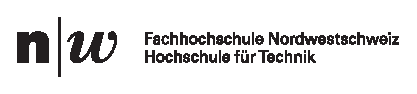
\includegraphics[height=12mm]{images/titlepage/fhnw.eps}%
        };
    \end{tikzpicture}



    % ---------------------------------------------------- %
    % The Text can  be set rather low in  the page without %
    % adjusting the top lengths.                           %
    % Backing up  and reseting these lengths  seems not to %
    % be necessary;  it appears  they are restored  at the %
    % end of the titlingpage environment.                  %
    % ---------------------------------------------------- %
    \setlength{\headsep}{0pt}
    \setlength{\headheight}{0pt}
    \setlength{\uppermargin}{4em}
    \checkandfixthelayout


    % ---------------------------------------------------- %
    % By   default,  centering   inside  the   titlingpage %
    % environment  will   center  with  respects   to  the %
    % typeblock. When  the  typeblock  is  centered,  this %
    % leads to  centered text  with respect to  the entire %
    % title  page. However,  When  the  typeblock  is  not %
    % centered, some adjustment is needed.                 %
    % See memman Chapter "Titles" for more information.    %
    % ---------------------------------------------------- %
    \calccentering{\unitlength}
    \begin{adjustwidth*}{\unitlength}{-\unitlength}


    % ---------------------------------------------------- %
    % Work some  magic to  automatically adjust  the hrule %
    % lengths to the length of the book title.             %
    %                                                      %
    % NOTE: The  font  size setting  needs  to  be in  the %
    % \mytitle  command, otherwise  \settolength will  not %
    % take it  into account  and will only  calculate with %
    % the default font size.                               %
    %                                                      %
    % NOTE  2: This mechanism  breaks if  the title  spans %
    % across multiple  lines. You're on  your own  in that %
    % case.                                                %
    % ---------------------------------------------------- %
    %\newcommand{\mytitle}{{\textbf{\fontsize{25mm}{1em}\selectfont Project Powerline}}} % default font
    \newcommand{\mytitle}{{\textbf{\fontsize{12mm}{1em}\selectfont Project Powerline}}}
    \newlength{\titlelength}            % Length of title text
    \settowidth{\titlelength}{\mytitle}
    \newcommand{\titlerulefactor}{1.2}  % Length of title rules, as a factor

    % ---------------------------------------------------- %
    % Set the title color                                  %
    % ---------------------------------------------------- %
    \newcommand{\titlecolor}{black}

    % ---------------------------------------------------- %
    % Put the title onto the page                          %
    % ---------------------------------------------------- %
    \textcolor{\titlecolor}{%
        \centering
        \rule{\titlerulefactor\titlelength}{1pt} \\
        \vspace*{4mm}
        \mytitle\\
        %\vspace*{5mm}
        \rule{\titlerulefactor\titlelength}{1pt} \\
        \vspace*{6mm}
        \fontsize{8mm}{1em}\selectfont Fachbericht \\
    }


    % ---------------------------------------------------- %
    % This is the end of the centering magic.              %
    % ---------------------------------------------------- %
    \end{adjustwidth*}


    % ---------------------------------------------------- %
    % Make  sure  this  is   not  put  into  \frontmatter, %
    % otherwise it will get a \frontmatter folio.          %
    % \cleardoblepage  is not  actually necessary  because %
    % it  is  automatically   called  by  the  titlingpage %
    % environment.                                         %
    % ---------------------------------------------------- %
    %\cleardoublepage

    %\setlength{\headsep}{\originallength}
    %\checkandfixthelayout
\end{titlingpage}


% -------------------------------------------------------- %
% See  the  memoir  documentation  for  what  specifically %
% frontmatter does. Among  other things, page  numbers are %
% set to roman numerals and chapter numbers are removed.   %
% -------------------------------------------------------- %
\frontmatter

% -------------------------------------------------------- %
% Comment out what's not needed, obviously.                %
% -------------------------------------------------------- %
%\begin{centering}
\vspace*{30mm}
\begin{tiny}
    \begin{tabular}{lll}
        Inhalt & \copyright~2016 & Marcel Heymann    \\
               &                 & Noah Hüsser       \\
               &                 & Raphael Frey      \\
               &                 & Dominik Keller    \\
               &                 & Marco Koch        \\
               &                 & Reto Nussbaumer   \\
               &                 & Francesco Rovelli \\
               &                 &                   \\
        Design & \copyright~2016 & Raphael Frey      \\
    \end{tabular}


    % ---------------------------------------------------- %
    % Having  this  in  a  tabular  is  a  bit  ugly,  but %
    % it  ensures alignment  and  limited paragraph  width %
    % without much effort.                                 %
    % ---------------------------------------------------- %
    \vspace{1em}
    \begin{tabular}{p{.9\textwidth}}
        \noindent  Erstellt  im  Fr\"uhlingssemester 2016  an  der  Hochschule
        f\"ur  Technik  der  Fachhochschule   Nordwestschweiz  im  Rahmen  des
        Modules   \emph{Projekt  4}   des   Studiengangs  \emph{Elektro-   und
        Informationstechnologie}. \\

        \\
        \iftoggle{paper}{%
            Dies     ist    die     Druckversion    dieses     Dokuments. Eine
            elektronische     Version      mit     farbig     hervorgehobenen,
            klickbaren   Links   ist   auf  den   abgegebenen   elektronischen
            Datentr\"agern  in  Anhang \ref{app:electronicStorage}  auf  Seite
            \pageref{app:electronicStorage}   zu   finden    oder   kann   bei
            \code{raphael.frey@students.fhnw.ch} angefordert werden.
        }{%
            Dies ist die elektronische  Ausf\"uhrung des Dokuments. Links sind
            farbig hervorgehoben und klickbar. Falls eine Version ohne farbige
            Akzentuierung erw\"unscht ist, kann diese bei
            \href{mailto:raphael.frey@students.fhnw.ch}{\code{raphael.frey@students.fhnw.ch}}
            angefordert werden.
            % internet links: blau
            % externe links: magenta
        }
        \\

        \\
        Dieses Dokument hat bisher \thecounttexruns~Kompiliervorg\"ange durchlaufen. \\
    \end{tabular}
    \vspace{1em}

    \begin{tabular}{>{\ttfamily}lrl}
        Version 0.1 & 06.05.2016 & Einleitung, Disposition \\
    \end{tabular}

    \vspace{1em}
    \begin{tabular}{l @{${}:{}$} l}
        Quelle Titelbild & \cite{ref:titlepage:pvanlage} \\
        Quelle Logo FHNW & \cite{ref:fhnwlogo}           \\
    \end{tabular}
\end{tiny}
%\\
%\footnotesize{\checkmark~\np~\noi~\partially} \\
%\\
%\large{\checkmark~\np~\noi~\partially} \\
%\\
%\checkmark~\np~\noi~\partially
%\end{centering}

% **************************************************************************** %
\chapter*{Abstract}
\label{chap:abstract}
% **************************************************************************** %
\enlargethispage{2em}

This project's  aim was to develop  a system for real-time  monitoring of each
panel  of a  photovoltaic facility.   The  system must  be cost-effective  and
should scale  from small single-household solutions  to large industrial-scale
solar  farms. Panels which  are not  operating at  full capacity  for whatever
reason (dirt, shade,  defects) must be detected and the  user informed so that
appropriate measures (cleaning, replacement) can be taken.

Monitoring  of  the  individual  photovoltaic modules  allows  the  facility's
operator to  optimally run  their solar  plant, thus  reducing losses  in both
power output and profit.

Current solutions for per-module monitoring  of solar facilities are expensive
and often left  out to save costs.   As alternative sources of  energy such as
wind and  solar power  grow in  importance, the overall  losses in  the energy
industry of power  and money incurred due to insufficient  monitoring of solar
facilities will become unsustainable.

Our  system  has  two  primary components: A  controller  which  is  installed
centrally  near  the  inverter  and  a  sensor  on  each  photovoltaic  panel.
Communication between the sensors and the  master is routed through the direct
current power  transmission line;  no additional wiring  is needed. A  coil is
used to couple the signal to the power line. In case of an error (e.g. a dirty
panel), an error message is sent to a user-configurable phone number.

Simulations for  various coupling methods  for a string  of 20 PV  panels have
been performed. Inductive  coupling at  non-resonance conditions results  in a
signal  level  of roughly  \SI{6}{\milli\volt}  peak-to-peak  at the  receiver
without  amplification. Operating  the  circuit  at resonance  yields  a  much
improved peak-to-peak  voltage of \SI{250}{\milli\volt} at  the receiver (also
without amplification), which is sufficient for our purposes.

A  frequency sweep  for  the coupling  coil has  been  measured and  inductive
behavior up to  \SI{20}{\mega\hertz} verified, thus ensuring that  the coil is
adaptable enough to allow the use of a vast range of frequencies as needed.

The system's components have been implemented. A  signal can be coupled to the
DC transmission line  and the sensor can perform  correct voltage measurements
and return that  data. Both the graphical user interface on  the master device
and its database back-end are functioning.

\vspace{2em}
\textbf{Key  words:}  photovoltaic  technology,  photovoltaic  module,  remote
monitoring, solar technology, PV cell, power efficiency, alternative energy,
powerline, communication, inductive coupling, capacitive coupling

%\include{frontmatter/dedication}
%\include{frontmatter/declaration}
%\include{frontmatter/acknowledgements}


% -------------------------------------------------------- %
% The starred versions do not make an entry for themselves %
% in the ToC, the unstarred versions do.                   %
% -------------------------------------------------------- %
{%
\enlargethispage{4em}
\tableofcontents*
}
%\newpage\listoffigures
%\newpage\listoftables


% -------------------------------------------------------- %
% Set page numbers to  arabic numerals, reset page counter %
% to 1, display  chapter numbers. See memoir documentation %
% for more information.                                    %
% -------------------------------------------------------- %
\mainmatter


% -------------------------------------------------------- %
% It is  advisable to use actually  meaningful chapter and %
% section names instead of generically numbered ones as in %
% this  example structure. That  way, their  place in  the %
% document is not directly tied to their file name, and it %
% is  possible to  restructure the  document (e.g.  move a %
% section  from one  chapter  to another,  or reorder  the %
% chapters)  without  needing  to adjust  file  names  and %
% similar shenanigans.                                     %
% -------------------------------------------------------- %
% **************************************************************************** %
\chapter{Einleitung}
\label{chap:einleitung}
% **************************************************************************** %

In Zeiten der Energiewende  sind Photovoltaikanlagen kein Nischenprodukt mehr.
Um die Abh\"angigkeit vom Erd\"ol  zu verringern, werden vielerorts Anlagen in
allen Gr\"ossen  gebaut; von kleinen Installationen  f\"ur Einfamilienh\"auser
bis zu Anlagen,  welche einem normalen Kraftwerk in Sachen  Leistung die Stirn
bieten k\"onnen.  Die  Sonnenstrahlung, welche kostenlos von  der Sonne kommt,
wird  in elektrische  Energie  umgewandelt  und kann  gleich  vor Ort  genutzt
werden.   PV-Anlagen sind  teuer,  weshalb  Anlagenbesitzer darauf  angewiesen
sind,  dass diese  den maximalen  Ertrag liefern. Das  ist in  der Regel  ohne
grossen  Aufwand  der  Fall.   Doch  es gibt  Umst\"ande,  unter  welchen  die
Effizienz  einer  Photovoltaikanlage  sich   erheblich  verringern  kann,  und
h\"aufig wird dies  nicht oder nur mit bedeutender  Verz\"ogerung bemerkt.  In
einer  Photovoltaikanlage werden  \"ublicherweise mehrere  PV-Module zu  einem
String zusammengefasst, indem sie  in Serie geschaltet werden. Dabei reduziert
ein abgeschattetes,  verschmutztes oder  gar defektes  Modul den  Strom dieser
Serieschaltung  und  beeintr\"achtigt somit  auch  die  Leistung des  gesamten
Strings und der Anlage stark. Dies hat grosse finanzielle Einbussen zur Folge.

Das Ziel des  Projektes P4 ist es, ein  PV-\"Uberwachungssystem zu entwickeln,
um bei  Szenarien wie dem  oben geschilderten Abhilfe zu  schaffen. Das System
soll aus  einer Sensorplatine  und einem zentralen  Meldeger\"at bestehen. Die
Sensorplatine wird  beim PV-Modul  eingebaut und \"uberwacht  dessen Spannung,
das   zentrale  Meldeger\"at   wird  im   Schaltschrank  beim   Wechselrichter
installiert. Die Kommunikation zwischen den  beiden Komponenten erfolgt \"uber
die  zur  Energie\"ubertragung  benutzte  DC-Leitung;  es  werden  also  keine
zus\"atzlichen Datenleitungen ben\"otigt.

Das Master-Ger\"at wertet die gemessenen  Spannungen der Module aus und l\"ost
beim Erkennen eines  fehlerhaften Moduls einen Alarm am  Ger\"at selbst, lokal
in der PV-Anlage via Relais (z.B. Sirene oder Warnlampe) und per SMS aus.  Das
System  soll m\"oglichst  energieeffizient  und kosteng\"unstig  sein, um  die
Wirtschaftlichkeit einer Photovoltaikanlage nicht zu verschlechtern.

Das  Hauptproblem  eines solchen  Systems  liegt  bei der  Signal\"ubertragung
\"uber  die  DC-Leitung  der   Photovoltaikanlage. Denn  die  Spannung  darauf
schwankt  zwischen 12  und  60  Volt an  der  Sensorplatine  und betr\"agt  am
Masterger\"at bis zu 1000 Volt. Auf dieser Leitung ein Signal zu \"ubertragen,
ist schwierig  und wird heutzutage  kaum gemacht. Unsere L\"osung  koppelt mit
einer Spule  und dem Effekt  der Induktivit\"at  ein Signal in  die DC-Leitung
ein, was uns das \"Ubertragen von  Daten erlaubt. Die Spule wird von einem auf
dem  Sensor  platzierten Mikrocontroller  gesteuert,  der  die Spannung  misst
und  die  Messdaten  zum  Versenden  vorbereitet. Das  Master-Ger\"at  besitzt
eine  grafische  Benutzeroberfl\"ache zur  Interaktion  mit  dem Benutzer  und
benutzt  eine Datenbank  zum Verwalten  der Messdaten.   Zudem ist  das System
darauf optimiert, m\"oglichst  wenig Leistung zu verbrauchen,  um nicht selbst
bedeutende Zusatzkosten im Betrieb zu verursachen.

Der   vorliegende  Bericht   stellt  die   technische  Dokumentation   unseres
Systems   dar. Das   Kapitel  \emph{\titleref{chap:uberblick}}   bietet   eine
kurze  Einf\"uhrung  in   die  Thematik  von  PV-Anlagen;   der  Aufbau  einer
\"ublichen  PV-Anlage  wird  kurz   erl\"autert,  um  anschliessend  die  oben
Problematik  von Leistungsverlusten  zu  untersuchen. Ebenfalls werden  einige
Grundinformationen  zur  Signalmodulation  gegeben.  Anschliessend  werden  in
den  Kapiteln  \emph{\titleref{chap:models}}  und  \emph{\titleref{chap:simu}}
verschiedene     verfolgte    L\"osungsvarianten     modelliert    und     mit
Simulationen  in  \code{LTspice}   untersucht. Die  schlussendlich  gew\"ahlte
L\"osung   mit    induktiver   Kopplung   ist   in    den   darauf   folgenden
Kapiteln  \emph{\titleref{chap:hardware}} und  \emph{\titleref{chap:software}}
dokumentiert.   Im   Kapitel  \emph{\titleref{chap:validierung}}   werden  das
entwickelte  System   und  seine   Komponenten  mit   Labormessungen  kritisch
untersucht, um letztlich  im \emph{\titleref{chap:fazit}} unseren Gesamterfolg
zu beurteilen und auch  Empfehlungen f\"ur zuk\"unftige Weiterentwicklungen zu
geben.

% **************************************************************************** %
\chapter{\"Uberblick}
\label{chap:uberblick}
% **************************************************************************** %

In   diesem  Kapitel   wird  zuerst   kurz  der   grundlegende  Aufbau   einer
PV-Anlage  erkl\"art,  um   sicherzustellen,  dass  keine  Missverst\"andnisse
beim   Interpretieren    der   nachfolgenden   Informationen   und    in   der
verwendeten Terminologie entstehen. Anschliessend werden Simulationsergebnisse
pr\"asentiert,   welche  verdeutlichen,   dass  die   Leistungsverluste  durch
einzelne,  nicht  optimal  funktionierende  Zellen  in  einer  grossen  Anlage
im  Bereich   von  mehreren  Kilowatt  liegen   k\"onnen. Daraus  leitet  sich
schlussendlich  die  Notwendigkeit   eines  \"Uberwachungssystems  ab. Zuletzt
werden verschiedene  Varianten vorgestellt,  wie ein  Signal auf  den DC-Strom
in   der  Leitung   zwischen   PV-Modul  und   Zentrale  aufmoduliert   werden
kann: Frequenzumtastung, Amplitudenumtastung  und \emph{On-off Keying}.


% ---------------------------------------------------------------------------- %
\section{Aufbau einer Photovoltaikanlage}
\label{sec:solaranlage:aufbau}
% ---------------------------------------------------------------------------- %

\enlargethispage{1em}
\begin{wrapfigure}{r}{0.35\textwidth}
    \centering
    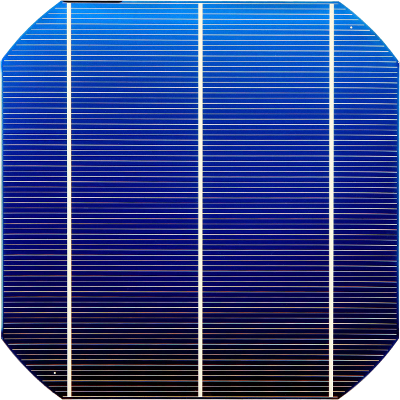
\includegraphics[width=0.30\textwidth]{images/solar-facility/cell--400px.png}
    \caption[Bild einer PV-Zelle]
    {Solarzelle, Frontalansicht \cite{ref:pvcell:wikipedia}}
    \label{fig:pvcell:front}
    \vspace*{-1em}
\end{wrapfigure}

Die   Grundbausteine    einer   Photovoltaikanlage   legen    die   PV-Zellen,
welche   aus   verschiedenen   Halbleitermaterialien   bestehen. Die   meisten
heutzutage  verwendeten  Zellen  werden aus  dem  Halbleitermaterial  Silizium
hergestellt. Siliziumzellen  sind in  verschiedenen Formfaktoren  verf\"ugbar;
g\"angige   Gr\"ossen    haben   ca.   zwischen    \SI{10}{\centi\meter}   und
\SI{15}{\centi\meter}  Kantenl\"ange.   Zum  mechanischen  Schutz  der  Zellen
sind  diese mit  einer durchsichtigen  Antireflexschicht \"uberzogen.   Die an
der  PV-Zelle  abgreifbare  Spannung betr\"agt  zwischen  \SI{0.5}{\volt}  und
\SI{0.8}{\volt} DC,  wobei die  Klemmenspannung einer  voll funktionsf\"ahigen
Zelle nur schwach von  der Lichteinstrahlung abh\"angig ist. Die Stromst\"arke
hingegen   ist  sehr   stark  von   der  Beleuchtungsst\"arke   abh\"angig. Je
nach    Sonneneinstrahlung   erreicht    eine   \SI{100}{\centi\meter\squared}
grosse   Siliziumzelle  eine   Stromst\"arke   von   bis  zu   \SI{2}{\ampere}
\cite{ref:pv:gesellschaftFuerSonnenenergie}. \fref{fig:pvcell:front} zeigt die
Frontansicht einer PV-Zelle.

\clearpage
\begin{wrapfigure}{l}{0.45\textwidth}
    \centering
    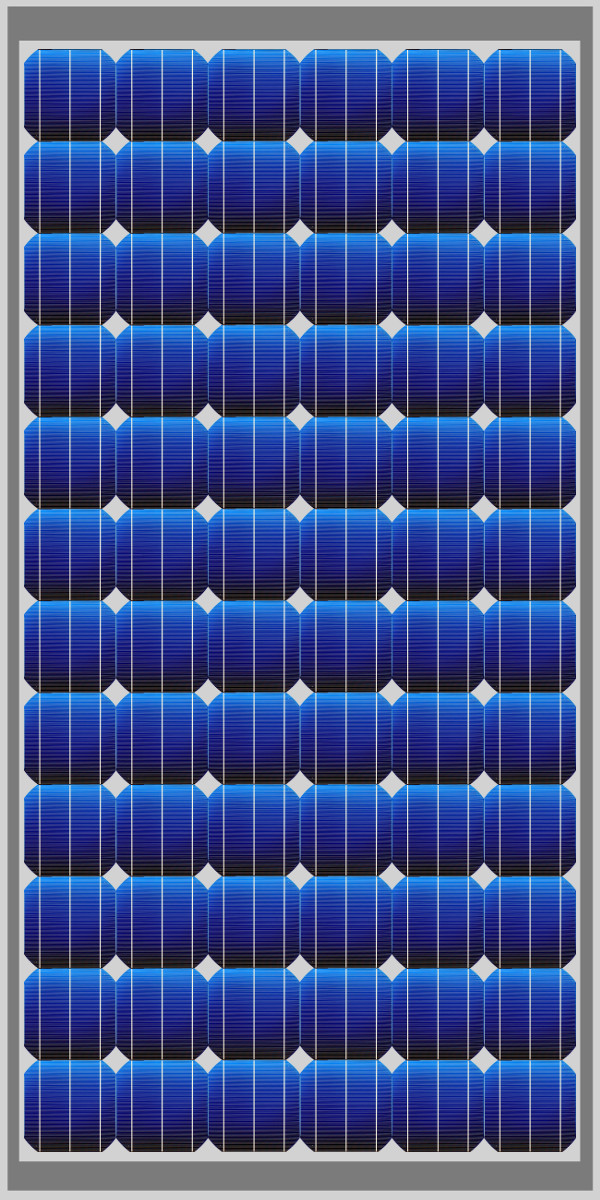
\includegraphics[width=0.4\textwidth]{images/solar-facility/pvmodule.jpeg}
    \caption[Bild eines PV-Moduls]
    {%
        Solarmodul,  zusammengesetzt  aus  72 Solarzellen  gem\"ass  Abbildung
        \ref{fig:pvcell:front}%
    }
    \label{fig:pvmodule}
    \vspace*{-1em}
\end{wrapfigure}


Die  in der  Praxis  \"ubliche  Baugruppe ist  nicht  die Solarzelle,  sondern
das   Photovoltaikmodul.\hfill   Um   \hfill   die   \hfill   Ausgangsspannung
\\und/oder  den  Ausgangsstrom  zu  erh\"ohen  und  um  diese  in  der  Praxis
besser  einsetzen   zu  k\"onnen,  werden  mehrere   Zellen  in  verschiedenen
Konfigurationen  miteinander zu  einem PV-Modul  verschaltet. Das Konzept  ist
schematisch dargestellt in Abbildung  \ref{fig:pvmodule}, die Eckdaten einiger
PV-Module sind als Beispiele  in Anhang \ref{app:commercial:modules} auf Seite
\pageref{app:commercial:modules} aufgef\"uhrt.

Zur  Erh\"ohung  des Ausgangsstroms  werden  Zellen  parallel geschaltet,  zur
Erh\"ohung  der  Ausgangsspannung werden  sie  in  Serie verbunden.   Je  nach
gew\"unschten Spezifikationen eines Moduls werden diese Ans\"atze einzeln oder
kombiniert angewandt.  In der Praxis \"ublich  sind Module mit 36, 72 oder 144
Zellen und  einer Ausgangsspannung  von \SI{12}{\volt}  bis \SI{60}{\volt}. In
Photovoltaikanlagen werden nur solche  ganzen Module eingesetzt; die einzelnen
Zellen  sind  f\"ur  Reparaturen  nicht  mehr  zug\"anglich. Die  elektrischen
Anschl\"usse befinden sich in kleinen  Kunststoffdosen auf der R\"uckseite der
Module (Beispiel in Abbildung \ref{fig:pvJunctionBox}) \cite{ref:pv:baunetz}.


Mehrere  identische  Module  werden  \"ublicherweise  mittels  Reihenschaltung
zu  einem  Modulstrang  verschaltet   (vereinfacht  dargestellt  in  Abbildung
\ref{fig:pvarray:gak:inverter}).  Dadurch wird  eine h\"ohere Ausgangsspannung
erzeugt, was die Umwandlung des Gleichstroms in

\begin{wrapfigure}{r}{0.35\textwidth}
    \centering
    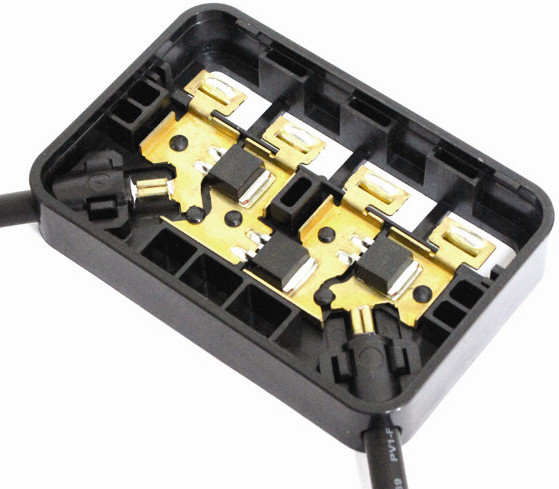
\includegraphics[width=0.3\textwidth]{images/solar-facility/pvJunctionBox.jpeg}
    \caption[Anschlussbox PV-Modul]{
        Anschlussbox   f\"ur   PV-Modul,   Montage   normalerweise   auf   der
        R\"uckseite  des  Moduls  \cite{ref:junctionBox}. Es  sind  auch  drei
        Freilaufdioden  erkennbar  (Abschnitt \ref{sec:shadedCells}  ab  Seite
        \pageref{sec:shadedCells})%
    }
    \label{fig:pvJunctionBox}
\end{wrapfigure}

\noindent   Wechselstrom   und   dessen   Einspeisung   ins   Wechselstromnetz
erleichtert. Die Ausgangsspannung eines  Modulstrangs darf gem\"ass Vorschrift
\SI{1000}{\volt} DC nicht \"uberschreiten, was  die Anzahl der in einem Strang
in Serie  geschalteten Module beschr\"ankt.  Module,  die an unterschiedlichen
Dachneigungen  montiert sind  oder die  unterschiedliche Ausrichtungen  haben,
sollten nie zu  einem Modulstrang zusammengeschaltet werden, da  sie nicht den
gleichen  Strom  produzieren  werden,  was die  Effizienz  des  Strangs  stark
reduziert. Ein einzelnes beschattetes  oder nicht einwandfrei funktionierendes
Modul beeintr\"achtigt die vom  gesamten Modulstrang abgegebene Leistung stark
(siehe n\"achster Abschnitt).

\clearpage
\enlargethispage{2em}
\begin{figure}[h!t]
    \centering
    \begin{tikzpicture}
        \begin{scope}[x={(0mm,\textwidth)},y={(0mm,-70mm)}]
            \node[inner sep=0pt,anchor=north west] at (0mm,0mm) {%
                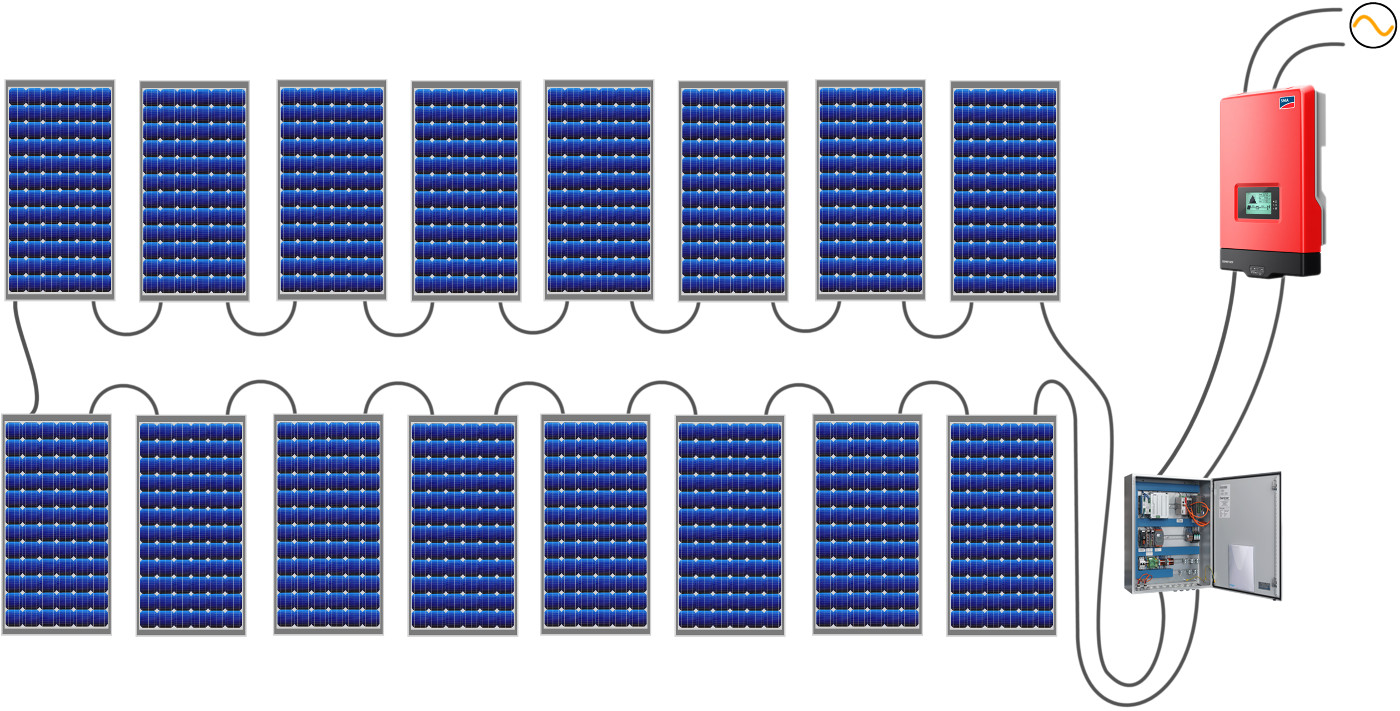
\includegraphics[width=\textwidth]{images/solar-facility/pvarray.jpeg}%
            };
            \node at (132mm,-55mm) {\small{GAK}};
            \node at (120mm,0mm) {\small{Wechselrichter}};
            \node at (55mm,-5mm) {\small{Modulstrang}};
        \end{scope}
    \end{tikzpicture}
    \caption[Modulstrang, \"Ubersichtsbild]{%
        Modulstrang aus 16 Modulen  gem\"ass Abbildung \ref{fig:pvmodule}, GAK
        und Wechselrichter. Bild des GAK  von \cite{ref:gak:gantner}, Bild des
        Wechselrichters von \cite{ref:inverter:sunnyboy}.%
    }
    \label{fig:pvarray:gak:inverter}
\end{figure}

Die    Umwandlung    der    Gleichspannung    in    Wechselspannung    erfolgt
mittels    Wechselrichter   (dargestellt    auf   der    rechten   Seite    in
Abbildung  \ref{fig:pvarray:gak:inverter}). Je  nach Anwendungsbereich  werden
unterschiedliche   Wechselrichter    eingesetzt,   aufgelistet    in   Tabelle
\ref{tab:inverters}.

\begin{table}[h!tb]
    \centering
    \caption{Arten von Wechselrichtern}
    \label{tab:inverters}
    \begin{tabular}{p{50mm}p{70mm}}
        \toprule
        \textbf{Modulwechselrichter}: &
        Ein  Wechselrichter,  welcher  den  Strom eines  einzelnen  Moduls  in
        Wechselstrom konvertiert. \\

        \textbf{Strangwechselrichter}: &
        Konvertiert den Strom eines Modulstrangs zu Wechselstrom. \\

        \textbf{Multistrangwechselrichter}: &
        Fasst   die   Gleichstr\"ome   mehrer  Modulstr\"ange   zusammen   und
        konvertiert diese zu Wechselstrom. \\

        \textbf{Zentralwechselrichter}: &
        Ein  einzelner Wechselrichter,  welcher den  Gleichstrom einer  ganzen
        Photovoltaikanlage in Wechselstrom umwandelt. Kommt haupts\"achlich in
        Grossanlagen zum Einsatz, bei denen alle Str\"ange die gleiche Neigung
        aufweisen und gleich ausgerichtet sind \cite{ref:pv:ratgeber}.\\
        \bottomrule
    \end{tabular}
\end{table}

Als Leitungsschutz gegen \"Uberstrom und Kurzschluss befindet sich unmittelbar
vor  dem   Wechselrichter  im  Gleichstromnetz   ein  Generatoranschlusskasten
(GAK). Dieser   dient   auch   zur    Trennung   der   gesamten   Anlage   vom
Netz. \"Ublicherweise  werden  GAK  und   Wechselrichter  am  selben  Standort
platziert.


% ---------------------------------------------------------------------------- %
\clearpage
\section{Leistungseinbr\"uche}
\label{sec:shadedCells}
% ---------------------------------------------------------------------------- %

In  diesem Abschnitt  werden einige  Simulationsergebnisse pr\"asentiert,  die
exemplarisch zeigen,  wie drastisch  die Leistungsf\"ahigkeit  einer PV-Anlage
aufgrund von kleinen Ursachen abnehmen kann.

Bei  der  Serieschaltung   von  Zellen  zu  einem  Modul   kann  bereits  eine
einzelne   nicht   voll   funktionsf\"ahige   Zelle   zu   starken   Einbussen
bei   der   Leistungsf\"ahigkeit  des   Moduls   f\"uhren\footnotemark. Dieser
Effekt  ist  in   den  Abbildungen  \ref{fig:simu:iv-curves:module:generic:3d}
und    \ref{fig:simu:iv-curves:module:generic}     gezeigt. Die    Abbildungen
basieren   auf    der   Simulation    eines   PV-Moduls,   welches    aus   72
in   Serie   geschalteten   Zellen   besteht   (die   zugeh\"orige   Schaltung
ist    in    Abbildung     \ref{fig:ltspice:iv:generic:module}    auf    Seite
\pageref{fig:ltspice:iv:generic:module}  dargestellt). Gibt   schon  nur  eine
von  72 Zellen  weniger  Strom  ab als  die  restlichen,  verringert sich  die
Leistungsf\"ahigkeit des Moduls betr\"achtlich. Der dabei von einem Modul noch
abgegebene Strom h\"angt wesentlich vom  Shunt-Widerstand des Modells bzw. vom
parallelen Innenwiderstand  der Zelle  ab (mehr zum  Modell einer  PV-Zelle in
Abschnitt \ref{sec:simu:model:cell} ab Seite \pageref{sec:simu:model:cell}).

\footnotetext{%
    Es   sei   an   dieser   Stelle  noch   erw\"ahnt,   dass   aufgrund   von
    Fertigungstoleranzen bei  realen Modulen  nat\"urlich niemals  alle Zellen
    den genau gleichen Arbeitspunkt  haben. Diese Effekte zu ber\"ucksichtigen
    w\"urde jedoch  die im  Rahmen dieses  Projekts zur  Verf\"ugung stehenden
    Ressourcen \"ubersteigen. Daher werden sie  f\"ur den Rest dieses Berichts
    nicht ber\"ucksichtigt.%
}

\begin{figure}[h!tb]
    \centering
    \begin{tikzpicture}
    \begin{scope}[x={(0mm,100mm)},y={(0mm,80mm)}]
        \begin{axis}[
            title = Strom{,} Spannung und Leistung eines PV-Moduls mit einer degradierten Zelle,
            %colormap/hot2,
            %colormap/cool,
            %colormap/viridis,
            colormap/temp,
            %height=80mm,
            width=110mm,
            grid=both,
            zmin=0,
            thick,
            xlabel=Spannung,
            ylabel=Strom,
            zlabel=Leistung,
            legend style={at={(0,-0.15)},anchor=north west},
            legend cell align=left,
        ]
            % 10A
            \addplot3[
                %draw=blue,
                draw=blue,
                scatter src = \thisrow{I(R3)},
            ] table[y expr=9] {data/iv-curves/generic-module/iv-generic--9a.dat};
            \addplot3[
                %draw=blue,
                draw=blue,
                scatter src = \thisrow{power},
            ] table[x expr=47] {data/iv-curves/generic-module/iv-generic--9a.dat};
            \addplot3[
                %draw=blue,
                draw=blue,
                scatter src = \thisrow{power},
            ] table[x expr=0] {data/iv-curves/generic-module/iv-generic--9a.dat};
            \addplot3[
                %draw=blue,
                draw=blue,
                scatter src = \thisrow{I(R3)},
            ] table[z expr=0] {data/iv-curves/generic-module/iv-generic--9a.dat};
            \addplot3[
                surf,
                shader=interp,
            ] table {data/iv-curves/generic-module/iv-generic--full-dataset.dat};
            \addplot3[
                draw=blue,
                very thick,
            ] table {data/iv-curves/generic-module/iv-generic--full-dataset.dat};
        \end{axis}
    \end{scope}
\end{tikzpicture}

    \caption
    [3d-Darstellung von Leistung, Spannung und Strom eines PV-Moduls]
    {%
        3D-Darstellung  von  Leistung,  Spannung und  Strom  eines  PV-Moduls.
        Abbildung    \ref{fig:simu:iv-curves:module:generic}    zeigt    diese
        Kurven  zweidimensional.    Die  zuge\"orige  \code{LTspice}-Schaltung
        ist   in  Abbildung   \ref{fig:ltspice:iv:generic:module}  auf   Seite
        \pageref{fig:ltspice:iv:generic:module} abgebildet.%
    }
    \label{fig:simu:iv-curves:module:generic:3d}
\end{figure}

\begin{figure}[h!tb]
    \centering
    \begin{tikzpicture}
   \begin{scope}[x={(0mm,0.95\textwidth)},y={(0mm,110mm)}]
       \begin{axis}[%
               title = Strom und Spannung eines PV-Moduls mit einer degradierten Zelle,
               height=50mm,
               width=0.95\textwidth,
               at={(0,55mm)},
               grid=both,
               xlabel=Spannung (\si{\volt}),
               ylabel=Strom (\si{\ampere}),
               xmin = 0,
               xmax = 48,
               legend cell align = right,
               legend style={at={(0.06,0.025)},anchor=south west},
               %axis y line*=left,
               %x unit=u,
               %change x base=true,
               %line width = 1pt,
               %thick,
               %x SI prefix=micro,
           ]
           \addplot[-,blue]  table[x=V(out), y=I(R3)] {data/iv-curves/generic-module/iv-generic--1a.dat};
           \addplot[-,magenta]    table[x=V(out), y=I(R3)] {data/iv-curves/generic-module/iv-generic--4a.dat};
           \addplot[-,teal] table[x=V(out), y=I(R3)] {data/iv-curves/generic-module/iv-generic--7a.dat};
           \addplot[-,cyan]    table[x=V(out), y=I(R3)] {data/iv-curves/generic-module/iv-generic--9a.dat};
           \legend{%
               11\%,
               44\%,
               78\%,
               100\%%
           }
        \end{axis}
        \begin{axis}[%
               title = Leistung eines PV-Moduls mit einer degradierten Zelle,
               height=50mm,
               width=0.95\textwidth,
               at={(0,0)},
               grid=both,
               xlabel=Spannung (\si{\volt}),
               ylabel=Leistung (\si{\watt}),
               xmin = 0,
               xmax = 48,
               legend style={at={(0.025,0.35)},anchor=south west},
           ]
           \addplot[-,blue]  table[x=V(out), y=power] {data/iv-curves/generic-module/iv-generic--1a.dat};
           \addplot[-,magenta]    table[x=V(out), y=power] {data/iv-curves/generic-module/iv-generic--4a.dat};
           \addplot[-,teal] table[x=V(out), y=power] {data/iv-curves/generic-module/iv-generic--7a.dat};
           \addplot[-,cyan]    table[x=V(out), y=power] {data/iv-curves/generic-module/iv-generic--9a.dat};
           \legend{%
               11\%,
               44\%,
               78\%,
               100\%%
           }
        \end{axis}
    \end{scope}
\end{tikzpicture}

    \caption[IV- und PV-Kurven eines PV-Moduls bei Leistungseinbruch]{%
        Verhalten   eines    Moduls   bei    Reduktion   des    Stroms   einer
        einzelnen   Zelle.
        Die   zuge\"orige  \code{LTspice}-Schaltung   ist
        in    Abbildung    \ref{fig:ltspice:iv:generic:module}    auf    Seite
        \pageref{fig:ltspice:iv:generic:module}    zu    finden.     Abbildung
        \ref{fig:simu:iv-curves:module:generic:3d}  zeigt  die  entsprechenden
        Zusammenh\"ange dreidimensional.%
    }
    \label{fig:simu:iv-curves:module:generic}
\end{figure}

Bei Serieschaltung von  mehreren PV-Modulen in einem Strang  kann bereits eine
einzige nicht  voll funktionsf\"ahige  Zelle in einem  Modul die  Leistung des
gesamten Strangs  stark beeintr\"achtigen.   Der gesamte  von einem  Modul und
somit auch von einem Strang (wegen Serieschaltung der Module) abgegebene Strom
h\"angt also stark von der schw\"achsten Zelle in der Schaltung ab.

Um  diesen  Effekt  zu  reduzieren,  werden  in  der  Praxis  in  jedem  Modul
jeweils  \"uber mehreren  Zellen  Freilaufdioden  (Engl. \emph{Bypass  Diode})
geschaltet. In  der  Anschlussbox  aus Abbildung  \ref{fig:pvJunctionBox}  von
Seite \pageref{fig:pvJunctionBox} sind drei Freilaufdioden sichtbar, womit zum
Beispiel drei  mal 24  Zellen mit je  einer Freilaufdiode  parallel geschaltet
werden k\"onnten. Aus Kostengr\"unden wird  nicht eine Freilaufdiode pro Zelle
verbaut, obwohl dies aus elektrotechnischer Sicht optimal w\"are.

\clearpage
Wird   ein   Strom   durch   eine   PV-Zelle   geleitet,   ohne   dass   diese
gen\"ugend   belichtet   ist,   findet    \"uber   der   Zelle   statt   eines
Spannungsanstiegs   wie    im   regul\"aren   Betrieb    ein   Spannungsabfall
statt,  was   bedeutet,  dass   der  durch   die  PV-Zelle   fliessende  Strom
in   der   Zelle   thermische   Verluste  produziert. Dies   ist   nicht   nur
ineffizient   und  un\"okonomisch,   sondern   kann   auch  eine   Brandgefahr
darstellen. Abbildung    \ref{fig:simu:iv-curves:array:generic}   zeigt    die
Simulation eines  Modulstrangs, in  dem keines  der Module  mit Freilaufdioden
versehen  ist. Wie  leicht  zu  erkennen  ist,  f\"allt  die  vom  Modulstrang
abgegebene Leistung bereits bei einer einzigen defekten Zelle (von 1440 Zellen
im gesamten Modulstrang!)  bedeutend ab. Gibt eine Zelle  lediglich noch einen
F\"unftel  des Stromes  der restlichen  Zellen  ab, f\"allt  die vom  gesamten
Strang  abgegebene Leistung  um etwa  einen Viertel. Da  die Sonneneintrahlung
verglichen mit  einer voll  funktionsf\"ahigen Anlage aber  unver\"andert ist,
produziert die Anlage eigentlich immer noch beinahge gleich viel Leistung. Die
nicht  mehr  zur  Verf\"ugung  stehende  Leistung  wird  aber  gr\"osstenteils
thermisch statt elektrisch abgegeben (daher auch Brandgefahr).


\begin{figure}[h!tb]
    \centering
    \begin{tikzpicture}
    \begin{scope}[x={(0mm,0.95\textwidth)},y={(0,110mm)}]
        \begin{axis}[%
                title = Strom eines Modulstrangs ohne Freilaufdioden,
                height=50mm,
                width=0.95\textwidth,
                at={(0,55mm)},
                grid=both,
                xlabel=Spannung (\si{\kilo\volt}),
                ylabel=Strom (\si{\ampere}),
                colormap/hot2,
                xmin = 0,
                xmax = 930,
                change x base=true,
                x SI prefix=kilo,
                legend cell align = right,
                legend style={at={(0.02,0.1)},anchor=south west},
            ]
            \addplot[-,blue]    table[x=V(out), y=I(R1)] {data/iv-curves/jac/stringNoD-IV-001pc.dat};
            \addplot[-,violet]  table[x=V(out), y=I(R1)] {data/iv-curves/jac/stringNoD-IV-022pc.dat};
            \addplot[-,teal]    table[x=V(out), y=I(R1)] {data/iv-curves/jac/stringNoD-IV-043pc.dat};
            \addplot[-,magenta] table[x=V(out), y=I(R1)] {data/iv-curves/jac/stringNoD-IV-065pc.dat};
            %\addplot[-,gray]   table[x=V(out), y=I(R1)] {data/iv-curves/jac/stringNoD-IV-086pc.dat};
            \addplot[-,cyan]    table[x=V(out), y=I(R1)] {data/iv-curves/jac/stringNoD-IV-100pc.dat};
            \legend{%
                1\%,
                22\%,
                43\%,
                65\%,
                100\%
            }

            %\addplot[-,purple]  table[x=V(out), y=I(R3)] {data/iv-curves/generic-array/iv-generic--1a.dat};
            %\addplot[-,teal]    table[x=V(out), y=I(R3)] {data/iv-curves/generic-array/iv-generic--4a.dat};
            %\addplot[-,magenta] table[x=V(out), y=I(R3)] {data/iv-curves/generic-array/iv-generic--7a.dat};
            %\addplot[-,blue]    table[x=V(out), y=I(R3)] {data/iv-curves/generic-array/iv-generic--9a.dat};

            %\addplot[-,color=blue] table {data/iv-curves/module-72cells-series--reference--all-ok.dat};
            %\addplot[-,color=teal] table {data/iv-curves/module-72cells-series--reference--ifail-5A.dat};
            %\addplot[-,color=magenta] table {data/iv-curves/module-72cells-series--reference--ifail-1A.dat};
        \end{axis}
        \begin{axis}[%
                title = Leistung eines Modulstrangs ohne Freilaufdioden,
                height=50mm,
                width=0.95\textwidth,
                at={(0,0)},
                grid=both,
                xlabel=Spannung (\si{\kilo\volt}),
                ylabel=Leistung (\si{\kilo\watt}),
                xmin = 0,
                xmax = 930,
                change x base=true,
                change y base=true,
                x SI prefix=kilo,
                y SI prefix=kilo,
                legend cell align = right,
                legend style={at={(0.02,0.30)},anchor=south west},
            ]
            \addplot[-,blue]    table[x=V(out), y=power] {data/iv-curves/jac/stringNoD-IV-001pc.dat};
            \addplot[-,violet]  table[x=V(out), y=power] {data/iv-curves/jac/stringNoD-IV-022pc.dat};
            \addplot[-,teal]    table[x=V(out), y=power] {data/iv-curves/jac/stringNoD-IV-043pc.dat};
            \addplot[-,magenta] table[x=V(out), y=power] {data/iv-curves/jac/stringNoD-IV-065pc.dat};
            %\addplot[-,gray]   table[x=V(out), y=power] {data/iv-curves/jac/stringNoD-IV-086pc.dat};
            \addplot[-,cyan]    table[x=V(out), y=power] {data/iv-curves/jac/stringNoD-IV-100pc.dat};
            \legend{%
                1\%,
                22\%,
                43\%,
                65\%,
                100\%
            }

            %\addplot[-,purple]  table[x=V(out), y=power] {data/iv-curves/generic-array/iv-generic--1a.dat};
            %\addplot[-,teal]    table[x=V(out), y=power] {data/iv-curves/generic-array/iv-generic--4a.dat};
            %\addplot[-,magenta] table[x=V(out), y=power] {data/iv-curves/generic-array/iv-generic--7a.dat};
            %\addplot[-,blue]    table[x=V(out), y=power] {data/iv-curves/generic-array/iv-generic--9a.dat};
        \end{axis}
    \end{scope}
\end{tikzpicture}

    \caption[%
        IV- und PV-Kurven eines Modulsstrangs bei Leistungseinbruch,
        keine Freilaufdioden%
    ]
    {%
        Verhalten       eines      Modulstrangs       ohne      Freilaufdioden
        bei     Reduktion     des     Stroms    einer     einzelnen     Zelle.
        Die      zugeh\"origen     \code{LTspice}-Schaltungen      sind     im
        Anhang       in       Abbildung       \ref{fig:ltspice:string:ivCurve}
        auf     Seite      \pageref{fig:ltspice:string:ivCurve}     und     in
        Abbildung      \ref{fig:ltspice:jacModule:NoDiode}      auf      Seite
        \pageref{fig:ltspice:jacModule:NoDiode} dokumentiert.%
    }
    \label{fig:simu:iv-curves:array:generic}
\end{figure}

\clearpage
Abbildung     \ref{fig:simu:iv-curves:array:generic:bypass}      zeigt     das
Verhalten       des      gleichen       Modulstranges      wie       Abbildung
\ref{fig:simu:iv-curves:array:generic} , nur dass nun zu jedem Modul noch eine
Freilaufdiode  parallel  geschaltet ist  (in  der  Praxis wird  wie  erw\"ahnt
mehr  als   eine  Freilaufdiode  pro   Modul  verwendet,  aber   f\"ur  unsere
Simulations-Szenarien ist eine Diode pro Modul ausreichend).

\begin{figure}[h!tb]
    \centering
    \begin{tikzpicture}
    \begin{scope}[x={(0mm,0.95\textwidth)},y={(0,110mm)}]
            \begin{axis}[%
                title=Stromg eines Modulstrangs mit Freilaufdioden,
                height=50mm,
                width=0.95\textwidth,
                at={(0,55mm)},
                grid=both,
                xlabel=Spannung (\si{\kilo\volt}),
                ylabel=Strom (\si{\ampere}),
                change x base=true,
                x SI prefix=kilo,
                xmin = 0,
                xmax = 930,
                legend cell align = right,
                legend style={at={(0.025,0.05)},anchor=south west},
            ]
            \addplot[-,blue]    table[x=V(out), y=I(R1)] {data/iv-curves/jac/string-IV-001pc-050pc.dat};
            \addplot[-,violet]  table[x=V(out), y=I(R1)] {data/iv-curves/jac/string-IV-001pc-075pc.dat};
            \addplot[-,teal]    table[x=V(out), y=I(R1)] {data/iv-curves/jac/string-IV-001pc-100pc.dat};
            \addplot[-,magenta] table[x=V(out), y=I(R1)] {data/iv-curves/jac/string-IV-043pc-050pc.dat};
            \addplot[-,gray]    table[x=V(out), y=I(R1)] {data/iv-curves/jac/string-IV-065pc-100pc.dat};
            \addplot[-,cyan]    table[x=V(out), y=I(R1)] {data/iv-curves/jac/string-IV-100pc-100pc.dat};
            \legend{%
                1\%{,} 50\%,
                1\%{,} 75\%,
                1\%{,} 100\%,
                43\%{,} 50\%,
                65\%{,} 100\%,
                100\%{,} 100\%%
            }
            %\addplot[-,purple]  table[x=V(out), y=I(R3)] {data/iv-curves/generic-array-bypass/iv-generic-bypass--1a.dat};
            %\addplot[-,teal]    table[x=V(out), y=I(R3)] {data/iv-curves/generic-array-bypass/iv-generic-bypass--4a.dat};
            %\addplot[-,magenta] table[x=V(out), y=I(R3)] {data/iv-curves/generic-array-bypass/iv-generic-bypass--7a.dat};
            %\addplot[-,blue]    table[x=V(out), y=I(R3)] {data/iv-curves/generic-array-bypass/iv-generic-bypass--9a.dat};
            %\addplot[-,color=blue] table {data/iv-curves/module-72cells-series--reference--all-ok.dat};
            %\addplot[-,color=teal] table {data/iv-curves/module-72cells-series--reference--ifail-5A.dat};
            %\addplot[-,color=magenta] table {data/iv-curves/module-72cells-series--reference--ifail-1A.dat};
        \end{axis}
        \begin{axis}[%
                title=Leistung eines Modulstrangs mit Freilaufdioden,
                height=50mm,
                width=0.95\textwidth,
                at={(0,0)},
                grid=both,
                xlabel=Spannung (\si{\kilo\volt}),
                ylabel=Leistung (\si{\kilo\watt}),
                change x base=true,
                change y base=true,
                x SI prefix=kilo,
                y SI prefix=kilo,
                xmin = 0,
                xmax = 930,
                legend cell align = right,
                legend style={at={(0.025,0.15)},anchor=south west},
            ]
            \addplot[-,blue]    table[x=V(out), y=power] {data/iv-curves/jac/string-IV-001pc-050pc.dat};
            \addplot[-,violet]  table[x=V(out), y=power] {data/iv-curves/jac/string-IV-001pc-075pc.dat};
            \addplot[-,teal]    table[x=V(out), y=power] {data/iv-curves/jac/string-IV-001pc-100pc.dat};
            \addplot[-,magenta] table[x=V(out), y=power] {data/iv-curves/jac/string-IV-043pc-050pc.dat};
            \addplot[-,gray]    table[x=V(out), y=power] {data/iv-curves/jac/string-IV-065pc-100pc.dat};
            \addplot[-,cyan]    table[x=V(out), y=power] {data/iv-curves/jac/string-IV-100pc-100pc.dat};
            \legend{%
                1\%{,} 50\%,
                1\%{,} 75\%,
                1\%{,} 100\%,
                43\%{,} 50\%,
                65\%{,} 100\%,
                100\%{,} 100\%%
            }

            %\addplot[-,purple]  table[x=V(out), y=power] {data/iv-curves/generic-array-bypass/iv-generic-bypass--1a.dat};
            %\addplot[-,teal]    table[x=V(out), y=power] {data/iv-curves/generic-array-bypass/iv-generic-bypass--4a.dat};
            %\addplot[-,magenta] table[x=V(out), y=power] {data/iv-curves/generic-array-bypass/iv-generic-bypass--7a.dat};
            %\addplot[-,blue]    table[x=V(out), y=power] {data/iv-curves/generic-array-bypass/iv-generic-bypass--9a.dat};
        \end{axis}
    \end{scope}
\end{tikzpicture}

    \caption[%
        IV- und PV-Kurven eines Modulsstrangs bei Leistungseinbruch,
        mit Freilaufdioden%
    ]
    {
        Verhalten   eines    Modulstrangs   bei   einer    Freilaufdiode   pro
        Modul. Es    werden     zwei    Zellen    in     zwei    verschiedenen
        Modulen   im   gesamten   Modulstrang   auf   reduzierte   Kapazit\"at
        gesetzt.   Die   Prozentangaben   in   der   Legende   beziehen   sich
        auf   die    Stromabgabe   der   zwei   Zellen    bezogen   auf   ihre
        maximale  Kapazit\"at. Die   zugeh\"origen  \code{LTspice}-Schaltungen
        sind   im   Anhang   in   Abbildung   \ref{fig:ltspice:string:ivCurve}
        auf     Seite      \pageref{fig:ltspice:string:ivCurve}     und     in
        Abbildung       \ref{fig:ltspice:jacModule:Diode}      auf       Seite
        \pageref{fig:ltspice:jacModule:Diode} dokumentiert.%
    }
    \label{fig:simu:iv-curves:array:generic:bypass}
\end{figure}

Die  Freilaufdioden leiten  den Strom  an den  nicht korrekt  funktionierenden
Zellstr\"angen  des  Moduls  vorbei,  und verhindern  somit,  dass  so  grosse
Verluste  wie  im  Szenario  ohne  Freilaufdioden  entstehen. Die  \"uber  der
Freilaufdiode abfallende  Vorw\"artsspannung ist  viel kleiner als  die \"uber
einem schlecht beleuchteten Modul abfallende Spannung.  Somit sind auch die in
der Freilaufdiode stattfindenden thermischen Verluste viel geringer.

Trotz  Freilaufdioden   k\"onnen  aber  auch   hier  die  Verluste   in  einer
grossen  PV-Anlage  sehr betr\"achtlich  werden,  da  eine solche  Anlage  aus
tausenden von  Strings bestehen kann. Somit sind  Freilaufdioden alleine nicht
ausreichend, um Leistungsverluste aufgrund  von nicht optimal funktionierenden
Zellen zufriedenstellend einzud\"ammen. Hier  schafft ein \"Uberwachungssystem
Abhilfe.


% ---------------------------------------------------------------------------- %
\clearpage
\section{Unser System}
\label{sec:ourSystem}
% ---------------------------------------------------------------------------- %

Unser   System  bietet,   neben  einer   benutzerfreundlichen  Bedienung   und
Inbetriebnahme  sowie  einer  einfachen  Integration  in  bestehende  Anlagen,
eine kosteng\"unstige  und energieeffiziente L\"osung f\"ur  die \"Uberwachung
von   Photovoltaikanlagen. Das   System   setzt   sich   zusammen   aus   zwei
Hauptkomponenten,   dem  Master-Ger\"at   und  den   jeweiligen  Sensoren. Die
schematische  Integration  des Systems  in  eine  PV-Anlage ist  in  Abbildung
\ref{fig:pvarray:gak:inverter:ourSystem} gezeigt.

\begin{figure}[h!t]
    \centering
    \begin{tikzpicture}
        \begin{scope}[red,x={(0mm,\textwidth)},y={(0mm,-70mm)}]
            \node[inner sep=0pt,anchor=north west] at (0mm,0mm) {%
                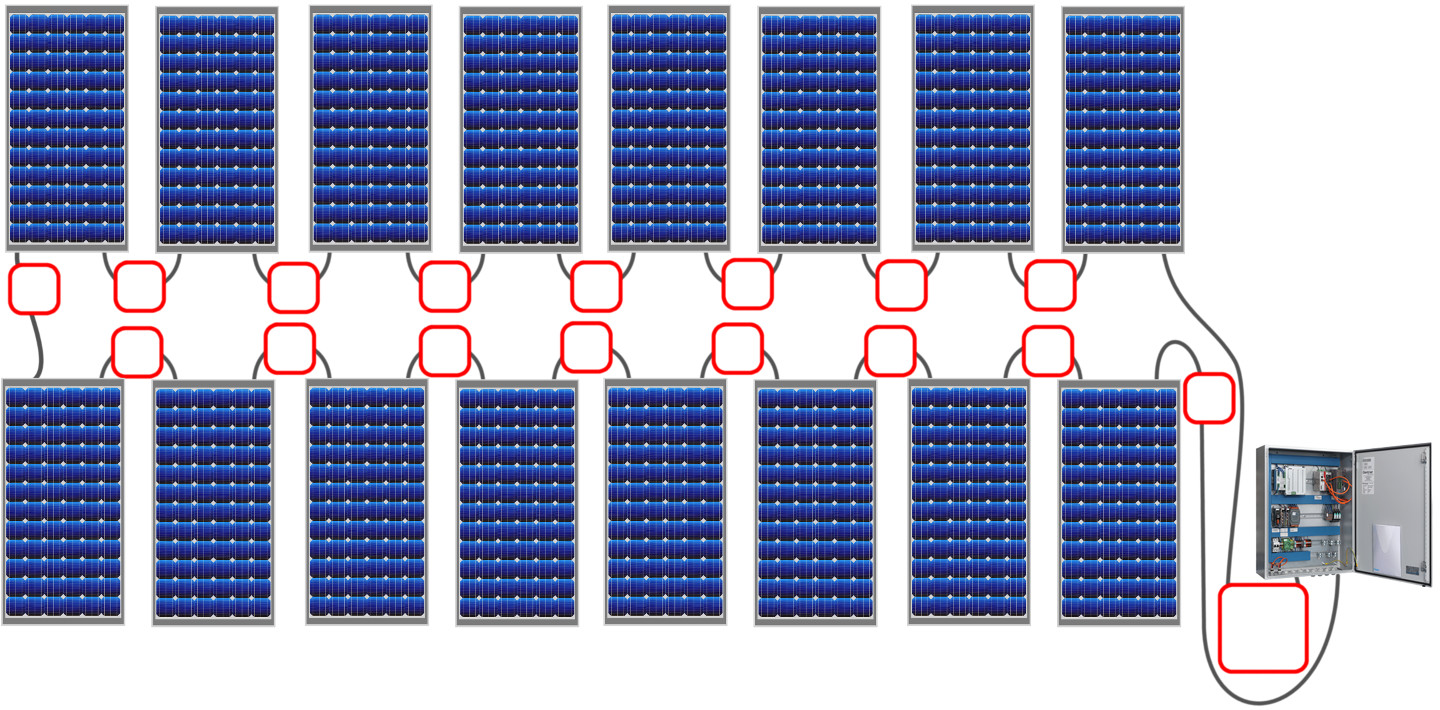
\includegraphics[width=\textwidth]{images/solar-facility/pvarray-ourSystem.jpeg}%
            };
            \node at (  3.5mm,-28.1mm) {S};
            \node at (13.75mm,-28mm) {S};
            \node at (28.75mm,-28mm) {S};
            \node at ( 43.5mm,-28mm) {S};
            \node at (58.25mm,-28mm) {S};
            \node at (72.75mm,-27.65mm) {S};
            \node at (87.75mm,-27.75mm) {S};
            \node at (102.25mm,-27.65mm) {S};

            \node at ( 13.5mm ,-34.4mm) {S};
            \node at ( 28.4mm ,-34.0mm) {S};
            \node at ( 43.45mm,-34.15mm) {S};
            \node at ( 57.2mm,-33.9mm) {S};
            \node at ( 71.75mm,-33.8mm) {S};
            \node at ( 86.65mm,-34.15mm) {S};
            \node at (102mm   ,-34.25mm) {S};

            \node at (117.7mm   ,-38.75mm) {S};

            \node at (122.75mm   ,-61.25mm) {\Huge M};
            %\node at (132mm,-55mm) {\small{GAK}};
            %\node at (120mm,0mm) {\small{Wechselrichter}};
            %\node at (55mm,-5mm) {\small{Modulstrang}};
        \end{scope}
    \end{tikzpicture}
    \caption[Modulstrang, \"Ubersichtsbild]{%
        Modulstrang mit je einem Sensor \textcolor{red}{S} pro Modul und einem
        \Master~\textcolor{red}{M} beim Generator-Anschlusskasten
    }
    \label{fig:pvarray:gak:inverter:ourSystem}
\end{figure}

Die    Installation   des    Master-Ger\"ates    erfolgt   im    zugeh\"origen
Schaltschrank. Das    Hutschienengeh\"ause    erm\"oglicht    eine    einfache
Installation in  bestehende oder  neue Schaltschr\"anke. Der Anschluss  an die
Energieversorgung  f\"ur das  Ger\"at selbst  wie auch  die Ankopplung  an die
DC-Leitungen  erfolgen im  Innern  des Schaltschrankes  und  werden von  einem
Elektroinstallateur ausgef\"uhrt.

Neben  dem   Klemmenanschluss  f\"ur   die  Energieversorgung  und   den  zwei
Relaisausg\"angen  f\"ur   externe  Alarmger\"ate   sieht  das   \Master~  die
Ankopplung der DC-Leitungen von bis zu drei Modulstr\"angen vor (einer gezeigt
in Abbildung \ref{fig:pvarray:gak:inverter:ourSystem}).

Ein  internes 2.5``  Touch-Display erm\"oglicht  eine einfache  Inbetriebnahme
und  eine benutzerfreundliche  Bedienung des  Systems. Alle Messresultate  der
Sensoren werden vom  \Master~ ausgewertet und dem Kunden  auf einer grafischen
Benutzeroberfl\"ache  dargestellt. Tritt ein  Fehler an  der Anlage  auf, wird
eine entsprechende Meldung auf dem Display angezeigt, die beiden Relais werden
bet\"atigt  und es  wird eine  Nachricht mittels  SMS versendet. Dadurch  wird
sichergestellt, dass der Kunde m\"oglichst schnell \"uber defekte PV-Module in
Kenntnis gesetzt wird.

\clearpage
Als Fehler werden folgende Ereignisse definiert:
\begin{itemize}
    \tightlist
    \item
        Eine defekte Zelle
    \item
        Eine dauerhaft verschmutzte Zelle
    \item
        Eine defekte Leitung
\end{itemize}

Kein Fehler soll in folgenden Situationen ausgel\"ost werden.
\begin{itemize}
    \tightlist
    \item
        Kurzzeitige Abschattungen (z.B. Vogel auf Zelle)
    \item
        Regelm\"assige Abschattungen,  die zu den  Umweltbedingungen geh\"oren
        (z.B. Baum, der t\"aglich abschattet)
    \item
        Nacht und schlechtes Wetter
    \item
        Anlage absichtlich ausser Betrieb genommen (z.B. Unterhaltsarbeiten)
\end{itemize}

F\"ur   die  Spannungsmessung   und   die   \"Ubertragung  der   Messresultate
sind  die   Sensoren  zust\"andig. Die   Installation  der   Sensoren  erfolgt
in  den   Anschlussdosen  auf  der  R\"uckseite   der  PV-Module. F\"ur  jedes
PV-Modul  ist   jeweils  ein   Sensor  zu   installieren,  wie   in  Abbildung
\ref{fig:pvarray:gak:inverter:ourSystem}  gezeigt. Eine zweiadrige  Verbindung
von der Sensorplatine  zu den Klemmen der Anschlussdose  ist zust\"andig f\"ur
die Energieversorgung  des Sensors. Die Einkopplung in  die DC-Leitung erfolgt
mit  einer  kleinen Induktionsspule,  durch  welche  die DC-Leitung  gef\"uhrt
wird. Dies erm\"oglicht das Kommunizieren mit dem \Master.


% ---------------------------------------------------------------------------- %
\section{Kommunikation \"uber DC-Leitung}
\label{sec:commDCLine}
% ---------------------------------------------------------------------------- %
\enlargethispage{2em}

Die Kommunikation  zwischen \Sensor~und \Master~\"uber die  DC-Leitung ist das
Herzst\"uck des Systems und das zu l\"osende Kernproblem des Projekts. Es sind
im Rahmen des  Projekts vier grunds\"atzliche Ans\"atze  untersucht worden, um
Daten  zwischen \Sensor~ und  \Master~  \"uber die  DC-Leitung  zu senden  und
empfangen.

\textbf{Frequency-shift keying}: Bei  der FSK (Frequenzumtastung  auf Deutsch)
wird  dem in  der Leitung  fliessenden Gleichstrom  ein (verh\"altnism\"assig)
kleines  Signal aufmoduliert,  welches  die  zu \"ubertragenden  Informationen
enth\"alt. Die Frequenz des aufmodulierten Anteils wird in diskreten Schritten
variiert und  jeweils einem  Symbol zugeordnet. Bei einer  bin\"aren Umsetzung
werden zwei Frequenzen benutzt; eine f\"ur \code{0} und eine f\"ur \code{1}.

\textbf{Amplitude-shift  keying}: Die  ASK (Amplitudenumtastung  auf  Deutsch)
benutzt statt verschiedenen Frequenzen unterschiedliche Amplituden, um Symbole
zu codieren.

\textbf{On-Off keying}: Bei  der OOK bedeuted die  Pr\"asenz einer Oszillation
auf  der  Leitung eine  \code{1},  die  Absenz von  Wechselstromanteilen  eine
logische  \code{0}. Eine   spezielle  Form   der  OOK,  welche   im  Abschnitt
\emph{\titleref{sec:simu:short}}  ab  Seite  \pageref{sec:simu:short}  genauer
untersucht  und  simuliert  wird,  benutzt  das  kontrollierte  Kurzschliessen
eines  PV-Moduls und  den  zugeh\"origen Spannungsabfall  zur Codierung  eines
Signals.

Abbildung   \ref{fig:modulation:concepts}   stellt    diese   vier   Varianten
vereinfacht dar,  zusammen mit dem  codierten Signal.  Aufgrund  der einfachen
Implementation haben  wird uns  f\"ur die Benutzung  einer OOK  mit Oszillator
entschieden.

\begin{figure}[h!tb]
    \centering
    %% Creator: Matplotlib, PGF backend
%%
%% To include the figure in your LaTeX document, write
%%   \input{<filename>.pgf}
%%
%% Make sure the required packages are loaded in your preamble
%%   \usepackage{pgf}
%%
%% Figures using additional raster images can only be included by \input if
%% they are in the same directory as the main LaTeX file. For loading figures
%% from other directories you can use the `import` package
%%   \usepackage{import}
%% and then include the figures with
%%   \import{<path to file>}{<filename>.pgf}
%%
%% Matplotlib used the following preamble
%%   \usepackage{fontspec}
%%   \setmainfont{Bitstream Vera Serif}
%%   \setsansfont{Bitstream Vera Sans}
%%   \setmonofont{Bitstream Vera Sans Mono}
%%
\begingroup%
\makeatletter%
\begin{pgfpicture}%
\pgfpathrectangle{\pgfpointorigin}{\pgfqpoint{5.100000in}{8.000000in}}%
\pgfusepath{use as bounding box, clip}%
\begin{pgfscope}%
\pgfsetbuttcap%
\pgfsetmiterjoin%
\pgfsetlinewidth{0.000000pt}%
\definecolor{currentstroke}{rgb}{0.000000,0.000000,0.000000}%
\pgfsetstrokecolor{currentstroke}%
\pgfsetstrokeopacity{0.000000}%
\pgfsetdash{}{0pt}%
\pgfpathmoveto{\pgfqpoint{0.000000in}{0.000000in}}%
\pgfpathlineto{\pgfqpoint{5.100000in}{0.000000in}}%
\pgfpathlineto{\pgfqpoint{5.100000in}{8.000000in}}%
\pgfpathlineto{\pgfqpoint{0.000000in}{8.000000in}}%
\pgfpathclose%
\pgfusepath{}%
\end{pgfscope}%
\begin{pgfscope}%
\pgfsetbuttcap%
\pgfsetmiterjoin%
\pgfsetlinewidth{0.000000pt}%
\definecolor{currentstroke}{rgb}{0.000000,0.000000,0.000000}%
\pgfsetstrokecolor{currentstroke}%
\pgfsetstrokeopacity{0.000000}%
\pgfsetdash{}{0pt}%
\pgfpathmoveto{\pgfqpoint{0.510000in}{6.541176in}}%
\pgfpathlineto{\pgfqpoint{4.845000in}{6.541176in}}%
\pgfpathlineto{\pgfqpoint{4.845000in}{7.600000in}}%
\pgfpathlineto{\pgfqpoint{0.510000in}{7.600000in}}%
\pgfpathclose%
\pgfusepath{}%
\end{pgfscope}%
\begin{pgfscope}%
\pgfpathrectangle{\pgfqpoint{0.510000in}{6.541176in}}{\pgfqpoint{4.335000in}{1.058824in}} %
\pgfusepath{clip}%
\pgfsetrectcap%
\pgfsetroundjoin%
\pgfsetlinewidth{0.501875pt}%
\definecolor{currentstroke}{rgb}{0.000000,0.000000,1.000000}%
\pgfsetstrokecolor{currentstroke}%
\pgfsetdash{}{0pt}%
\pgfpathmoveto{\pgfqpoint{0.510000in}{6.629412in}}%
\pgfpathlineto{\pgfqpoint{1.593750in}{6.629412in}}%
\pgfusepath{stroke}%
\end{pgfscope}%
\begin{pgfscope}%
\pgfpathrectangle{\pgfqpoint{0.510000in}{6.541176in}}{\pgfqpoint{4.335000in}{1.058824in}} %
\pgfusepath{clip}%
\pgfsetrectcap%
\pgfsetroundjoin%
\pgfsetlinewidth{0.501875pt}%
\definecolor{currentstroke}{rgb}{0.501961,0.501961,0.501961}%
\pgfsetstrokecolor{currentstroke}%
\pgfsetdash{}{0pt}%
\pgfpathmoveto{\pgfqpoint{1.593750in}{6.629412in}}%
\pgfpathlineto{\pgfqpoint{1.593750in}{7.511765in}}%
\pgfusepath{stroke}%
\end{pgfscope}%
\begin{pgfscope}%
\pgfpathrectangle{\pgfqpoint{0.510000in}{6.541176in}}{\pgfqpoint{4.335000in}{1.058824in}} %
\pgfusepath{clip}%
\pgfsetrectcap%
\pgfsetroundjoin%
\pgfsetlinewidth{0.501875pt}%
\definecolor{currentstroke}{rgb}{1.000000,0.000000,1.000000}%
\pgfsetstrokecolor{currentstroke}%
\pgfsetdash{}{0pt}%
\pgfpathmoveto{\pgfqpoint{1.593750in}{7.511765in}}%
\pgfpathlineto{\pgfqpoint{2.677500in}{7.511765in}}%
\pgfusepath{stroke}%
\end{pgfscope}%
\begin{pgfscope}%
\pgfpathrectangle{\pgfqpoint{0.510000in}{6.541176in}}{\pgfqpoint{4.335000in}{1.058824in}} %
\pgfusepath{clip}%
\pgfsetrectcap%
\pgfsetroundjoin%
\pgfsetlinewidth{0.501875pt}%
\definecolor{currentstroke}{rgb}{0.501961,0.501961,0.501961}%
\pgfsetstrokecolor{currentstroke}%
\pgfsetdash{}{0pt}%
\pgfpathmoveto{\pgfqpoint{2.677500in}{7.511765in}}%
\pgfpathlineto{\pgfqpoint{2.677500in}{6.629412in}}%
\pgfusepath{stroke}%
\end{pgfscope}%
\begin{pgfscope}%
\pgfpathrectangle{\pgfqpoint{0.510000in}{6.541176in}}{\pgfqpoint{4.335000in}{1.058824in}} %
\pgfusepath{clip}%
\pgfsetrectcap%
\pgfsetroundjoin%
\pgfsetlinewidth{0.501875pt}%
\definecolor{currentstroke}{rgb}{0.000000,0.000000,1.000000}%
\pgfsetstrokecolor{currentstroke}%
\pgfsetdash{}{0pt}%
\pgfpathmoveto{\pgfqpoint{2.677500in}{6.629412in}}%
\pgfpathlineto{\pgfqpoint{3.761250in}{6.629412in}}%
\pgfusepath{stroke}%
\end{pgfscope}%
\begin{pgfscope}%
\pgfpathrectangle{\pgfqpoint{0.510000in}{6.541176in}}{\pgfqpoint{4.335000in}{1.058824in}} %
\pgfusepath{clip}%
\pgfsetrectcap%
\pgfsetroundjoin%
\pgfsetlinewidth{0.501875pt}%
\definecolor{currentstroke}{rgb}{0.501961,0.501961,0.501961}%
\pgfsetstrokecolor{currentstroke}%
\pgfsetdash{}{0pt}%
\pgfpathmoveto{\pgfqpoint{3.761250in}{6.629412in}}%
\pgfpathlineto{\pgfqpoint{3.761250in}{7.511765in}}%
\pgfusepath{stroke}%
\end{pgfscope}%
\begin{pgfscope}%
\pgfpathrectangle{\pgfqpoint{0.510000in}{6.541176in}}{\pgfqpoint{4.335000in}{1.058824in}} %
\pgfusepath{clip}%
\pgfsetrectcap%
\pgfsetroundjoin%
\pgfsetlinewidth{0.501875pt}%
\definecolor{currentstroke}{rgb}{1.000000,0.000000,1.000000}%
\pgfsetstrokecolor{currentstroke}%
\pgfsetdash{}{0pt}%
\pgfpathmoveto{\pgfqpoint{3.761250in}{7.511765in}}%
\pgfpathlineto{\pgfqpoint{4.845000in}{7.511765in}}%
\pgfusepath{stroke}%
\end{pgfscope}%
\begin{pgfscope}%
\pgfsetrectcap%
\pgfsetmiterjoin%
\pgfsetlinewidth{0.501875pt}%
\definecolor{currentstroke}{rgb}{0.000000,0.000000,0.000000}%
\pgfsetstrokecolor{currentstroke}%
\pgfsetdash{}{0pt}%
\pgfpathmoveto{\pgfqpoint{0.510000in}{7.600000in}}%
\pgfpathlineto{\pgfqpoint{4.845000in}{7.600000in}}%
\pgfusepath{stroke}%
\end{pgfscope}%
\begin{pgfscope}%
\pgfsetrectcap%
\pgfsetmiterjoin%
\pgfsetlinewidth{0.501875pt}%
\definecolor{currentstroke}{rgb}{0.000000,0.000000,0.000000}%
\pgfsetstrokecolor{currentstroke}%
\pgfsetdash{}{0pt}%
\pgfpathmoveto{\pgfqpoint{0.510000in}{6.541176in}}%
\pgfpathlineto{\pgfqpoint{0.510000in}{7.600000in}}%
\pgfusepath{stroke}%
\end{pgfscope}%
\begin{pgfscope}%
\pgfsetrectcap%
\pgfsetmiterjoin%
\pgfsetlinewidth{0.501875pt}%
\definecolor{currentstroke}{rgb}{0.000000,0.000000,0.000000}%
\pgfsetstrokecolor{currentstroke}%
\pgfsetdash{}{0pt}%
\pgfpathmoveto{\pgfqpoint{0.510000in}{6.541176in}}%
\pgfpathlineto{\pgfqpoint{4.845000in}{6.541176in}}%
\pgfusepath{stroke}%
\end{pgfscope}%
\begin{pgfscope}%
\pgfsetrectcap%
\pgfsetmiterjoin%
\pgfsetlinewidth{0.501875pt}%
\definecolor{currentstroke}{rgb}{0.000000,0.000000,0.000000}%
\pgfsetstrokecolor{currentstroke}%
\pgfsetdash{}{0pt}%
\pgfpathmoveto{\pgfqpoint{4.845000in}{6.541176in}}%
\pgfpathlineto{\pgfqpoint{4.845000in}{7.600000in}}%
\pgfusepath{stroke}%
\end{pgfscope}%
\begin{pgfscope}%
\pgftext[x=2.677500in,y=6.471732in,,top]{\rmfamily\fontsize{9.000000}{10.800000}\selectfont Zeit}%
\end{pgfscope}%
\begin{pgfscope}%
\pgfsetbuttcap%
\pgfsetroundjoin%
\definecolor{currentfill}{rgb}{0.000000,0.000000,0.000000}%
\pgfsetfillcolor{currentfill}%
\pgfsetlinewidth{0.501875pt}%
\definecolor{currentstroke}{rgb}{0.000000,0.000000,0.000000}%
\pgfsetstrokecolor{currentstroke}%
\pgfsetdash{}{0pt}%
\pgfsys@defobject{currentmarker}{\pgfqpoint{0.000000in}{0.000000in}}{\pgfqpoint{0.055556in}{0.000000in}}{%
\pgfpathmoveto{\pgfqpoint{0.000000in}{0.000000in}}%
\pgfpathlineto{\pgfqpoint{0.055556in}{0.000000in}}%
\pgfusepath{stroke,fill}%
}%
\begin{pgfscope}%
\pgfsys@transformshift{0.510000in}{6.629412in}%
\pgfsys@useobject{currentmarker}{}%
\end{pgfscope}%
\end{pgfscope}%
\begin{pgfscope}%
\pgfsetbuttcap%
\pgfsetroundjoin%
\definecolor{currentfill}{rgb}{0.000000,0.000000,0.000000}%
\pgfsetfillcolor{currentfill}%
\pgfsetlinewidth{0.501875pt}%
\definecolor{currentstroke}{rgb}{0.000000,0.000000,0.000000}%
\pgfsetstrokecolor{currentstroke}%
\pgfsetdash{}{0pt}%
\pgfsys@defobject{currentmarker}{\pgfqpoint{-0.055556in}{0.000000in}}{\pgfqpoint{0.000000in}{0.000000in}}{%
\pgfpathmoveto{\pgfqpoint{0.000000in}{0.000000in}}%
\pgfpathlineto{\pgfqpoint{-0.055556in}{0.000000in}}%
\pgfusepath{stroke,fill}%
}%
\begin{pgfscope}%
\pgfsys@transformshift{4.845000in}{6.629412in}%
\pgfsys@useobject{currentmarker}{}%
\end{pgfscope}%
\end{pgfscope}%
\begin{pgfscope}%
\pgftext[x=0.454444in,y=6.629412in,right,]{\rmfamily\fontsize{9.000000}{10.800000}\selectfont \(\displaystyle 0\)}%
\end{pgfscope}%
\begin{pgfscope}%
\pgfsetbuttcap%
\pgfsetroundjoin%
\definecolor{currentfill}{rgb}{0.000000,0.000000,0.000000}%
\pgfsetfillcolor{currentfill}%
\pgfsetlinewidth{0.501875pt}%
\definecolor{currentstroke}{rgb}{0.000000,0.000000,0.000000}%
\pgfsetstrokecolor{currentstroke}%
\pgfsetdash{}{0pt}%
\pgfsys@defobject{currentmarker}{\pgfqpoint{0.000000in}{0.000000in}}{\pgfqpoint{0.055556in}{0.000000in}}{%
\pgfpathmoveto{\pgfqpoint{0.000000in}{0.000000in}}%
\pgfpathlineto{\pgfqpoint{0.055556in}{0.000000in}}%
\pgfusepath{stroke,fill}%
}%
\begin{pgfscope}%
\pgfsys@transformshift{0.510000in}{7.511765in}%
\pgfsys@useobject{currentmarker}{}%
\end{pgfscope}%
\end{pgfscope}%
\begin{pgfscope}%
\pgfsetbuttcap%
\pgfsetroundjoin%
\definecolor{currentfill}{rgb}{0.000000,0.000000,0.000000}%
\pgfsetfillcolor{currentfill}%
\pgfsetlinewidth{0.501875pt}%
\definecolor{currentstroke}{rgb}{0.000000,0.000000,0.000000}%
\pgfsetstrokecolor{currentstroke}%
\pgfsetdash{}{0pt}%
\pgfsys@defobject{currentmarker}{\pgfqpoint{-0.055556in}{0.000000in}}{\pgfqpoint{0.000000in}{0.000000in}}{%
\pgfpathmoveto{\pgfqpoint{0.000000in}{0.000000in}}%
\pgfpathlineto{\pgfqpoint{-0.055556in}{0.000000in}}%
\pgfusepath{stroke,fill}%
}%
\begin{pgfscope}%
\pgfsys@transformshift{4.845000in}{7.511765in}%
\pgfsys@useobject{currentmarker}{}%
\end{pgfscope}%
\end{pgfscope}%
\begin{pgfscope}%
\pgftext[x=0.454444in,y=7.511765in,right,]{\rmfamily\fontsize{9.000000}{10.800000}\selectfont \(\displaystyle 1\)}%
\end{pgfscope}%
\begin{pgfscope}%
\pgftext[x=0.320764in,y=7.070588in,,bottom,rotate=90.000000]{\rmfamily\fontsize{9.000000}{10.800000}\selectfont Symbol}%
\end{pgfscope}%
\begin{pgfscope}%
\pgftext[x=2.677500in,y=7.669444in,,base]{\rmfamily\fontsize{11.000000}{13.200000}\selectfont Daten}%
\end{pgfscope}%
\begin{pgfscope}%
\pgfsetbuttcap%
\pgfsetmiterjoin%
\pgfsetlinewidth{0.000000pt}%
\definecolor{currentstroke}{rgb}{0.000000,0.000000,0.000000}%
\pgfsetstrokecolor{currentstroke}%
\pgfsetstrokeopacity{0.000000}%
\pgfsetdash{}{0pt}%
\pgfpathmoveto{\pgfqpoint{0.510000in}{5.005882in}}%
\pgfpathlineto{\pgfqpoint{4.845000in}{5.005882in}}%
\pgfpathlineto{\pgfqpoint{4.845000in}{6.064706in}}%
\pgfpathlineto{\pgfqpoint{0.510000in}{6.064706in}}%
\pgfpathclose%
\pgfusepath{}%
\end{pgfscope}%
\begin{pgfscope}%
\pgfpathrectangle{\pgfqpoint{0.510000in}{5.005882in}}{\pgfqpoint{4.335000in}{1.058824in}} %
\pgfusepath{clip}%
\pgfsetrectcap%
\pgfsetroundjoin%
\pgfsetlinewidth{0.501875pt}%
\definecolor{currentstroke}{rgb}{0.000000,0.000000,1.000000}%
\pgfsetstrokecolor{currentstroke}%
\pgfsetdash{}{0pt}%
\pgfpathmoveto{\pgfqpoint{0.510000in}{5.054011in}}%
\pgfpathlineto{\pgfqpoint{0.515424in}{5.054962in}}%
\pgfpathlineto{\pgfqpoint{0.521933in}{5.058611in}}%
\pgfpathlineto{\pgfqpoint{0.528442in}{5.064973in}}%
\pgfpathlineto{\pgfqpoint{0.536036in}{5.075777in}}%
\pgfpathlineto{\pgfqpoint{0.544715in}{5.092478in}}%
\pgfpathlineto{\pgfqpoint{0.554478in}{5.116611in}}%
\pgfpathlineto{\pgfqpoint{0.565327in}{5.149698in}}%
\pgfpathlineto{\pgfqpoint{0.578345in}{5.197392in}}%
\pgfpathlineto{\pgfqpoint{0.593532in}{5.262661in}}%
\pgfpathlineto{\pgfqpoint{0.611974in}{5.353039in}}%
\pgfpathlineto{\pgfqpoint{0.636926in}{5.487696in}}%
\pgfpathlineto{\pgfqpoint{0.683574in}{5.741091in}}%
\pgfpathlineto{\pgfqpoint{0.702016in}{5.828731in}}%
\pgfpathlineto{\pgfqpoint{0.717203in}{5.891027in}}%
\pgfpathlineto{\pgfqpoint{0.730221in}{5.935729in}}%
\pgfpathlineto{\pgfqpoint{0.741070in}{5.966062in}}%
\pgfpathlineto{\pgfqpoint{0.750833in}{5.987553in}}%
\pgfpathlineto{\pgfqpoint{0.759512in}{6.001801in}}%
\pgfpathlineto{\pgfqpoint{0.767106in}{6.010401in}}%
\pgfpathlineto{\pgfqpoint{0.773615in}{6.014844in}}%
\pgfpathlineto{\pgfqpoint{0.780124in}{6.016556in}}%
\pgfpathlineto{\pgfqpoint{0.785548in}{6.015890in}}%
\pgfpathlineto{\pgfqpoint{0.792057in}{6.012583in}}%
\pgfpathlineto{\pgfqpoint{0.798566in}{6.006558in}}%
\pgfpathlineto{\pgfqpoint{0.806160in}{5.996141in}}%
\pgfpathlineto{\pgfqpoint{0.814839in}{5.979870in}}%
\pgfpathlineto{\pgfqpoint{0.824602in}{5.956197in}}%
\pgfpathlineto{\pgfqpoint{0.835450in}{5.923590in}}%
\pgfpathlineto{\pgfqpoint{0.847384in}{5.880658in}}%
\pgfpathlineto{\pgfqpoint{0.861486in}{5.821481in}}%
\pgfpathlineto{\pgfqpoint{0.878844in}{5.738350in}}%
\pgfpathlineto{\pgfqpoint{0.901625in}{5.617377in}}%
\pgfpathlineto{\pgfqpoint{0.959122in}{5.306544in}}%
\pgfpathlineto{\pgfqpoint{0.976479in}{5.226511in}}%
\pgfpathlineto{\pgfqpoint{0.991667in}{5.166610in}}%
\pgfpathlineto{\pgfqpoint{1.004685in}{5.124282in}}%
\pgfpathlineto{\pgfqpoint{1.015533in}{5.096114in}}%
\pgfpathlineto{\pgfqpoint{1.025297in}{5.076686in}}%
\pgfpathlineto{\pgfqpoint{1.033975in}{5.064340in}}%
\pgfpathlineto{\pgfqpoint{1.041569in}{5.057443in}}%
\pgfpathlineto{\pgfqpoint{1.048078in}{5.054477in}}%
\pgfpathlineto{\pgfqpoint{1.053502in}{5.054096in}}%
\pgfpathlineto{\pgfqpoint{1.058926in}{5.055619in}}%
\pgfpathlineto{\pgfqpoint{1.065435in}{5.059948in}}%
\pgfpathlineto{\pgfqpoint{1.071944in}{5.066984in}}%
\pgfpathlineto{\pgfqpoint{1.079538in}{5.078559in}}%
\pgfpathlineto{\pgfqpoint{1.088217in}{5.096114in}}%
\pgfpathlineto{\pgfqpoint{1.097980in}{5.121164in}}%
\pgfpathlineto{\pgfqpoint{1.108829in}{5.155200in}}%
\pgfpathlineto{\pgfqpoint{1.121847in}{5.203918in}}%
\pgfpathlineto{\pgfqpoint{1.137035in}{5.270193in}}%
\pgfpathlineto{\pgfqpoint{1.155477in}{5.361476in}}%
\pgfpathlineto{\pgfqpoint{1.182598in}{5.508821in}}%
\pgfpathlineto{\pgfqpoint{1.223821in}{5.732846in}}%
\pgfpathlineto{\pgfqpoint{1.243348in}{5.826326in}}%
\pgfpathlineto{\pgfqpoint{1.258536in}{5.888981in}}%
\pgfpathlineto{\pgfqpoint{1.271554in}{5.934042in}}%
\pgfpathlineto{\pgfqpoint{1.283487in}{5.967403in}}%
\pgfpathlineto{\pgfqpoint{1.293251in}{5.988579in}}%
\pgfpathlineto{\pgfqpoint{1.301929in}{6.002537in}}%
\pgfpathlineto{\pgfqpoint{1.309523in}{6.010875in}}%
\pgfpathlineto{\pgfqpoint{1.316032in}{6.015091in}}%
\pgfpathlineto{\pgfqpoint{1.322541in}{6.016575in}}%
\pgfpathlineto{\pgfqpoint{1.327965in}{6.015719in}}%
\pgfpathlineto{\pgfqpoint{1.334474in}{6.012184in}}%
\pgfpathlineto{\pgfqpoint{1.340983in}{6.005934in}}%
\pgfpathlineto{\pgfqpoint{1.348577in}{5.995259in}}%
\pgfpathlineto{\pgfqpoint{1.357256in}{5.978701in}}%
\pgfpathlineto{\pgfqpoint{1.367020in}{5.954721in}}%
\pgfpathlineto{\pgfqpoint{1.377868in}{5.921794in}}%
\pgfpathlineto{\pgfqpoint{1.390886in}{5.874272in}}%
\pgfpathlineto{\pgfqpoint{1.406074in}{5.809173in}}%
\pgfpathlineto{\pgfqpoint{1.424516in}{5.718949in}}%
\pgfpathlineto{\pgfqpoint{1.449467in}{5.584398in}}%
\pgfpathlineto{\pgfqpoint{1.497200in}{5.325402in}}%
\pgfpathlineto{\pgfqpoint{1.515642in}{5.238271in}}%
\pgfpathlineto{\pgfqpoint{1.530830in}{5.176519in}}%
\pgfpathlineto{\pgfqpoint{1.543848in}{5.132358in}}%
\pgfpathlineto{\pgfqpoint{1.554696in}{5.102521in}}%
\pgfpathlineto{\pgfqpoint{1.564459in}{5.081503in}}%
\pgfpathlineto{\pgfqpoint{1.573138in}{5.067691in}}%
\pgfpathlineto{\pgfqpoint{1.580732in}{5.059483in}}%
\pgfpathlineto{\pgfqpoint{1.587241in}{5.055381in}}%
\pgfpathlineto{\pgfqpoint{1.593750in}{5.054011in}}%
\pgfpathlineto{\pgfqpoint{1.593750in}{5.054011in}}%
\pgfusepath{stroke}%
\end{pgfscope}%
\begin{pgfscope}%
\pgfpathrectangle{\pgfqpoint{0.510000in}{5.005882in}}{\pgfqpoint{4.335000in}{1.058824in}} %
\pgfusepath{clip}%
\pgfsetrectcap%
\pgfsetroundjoin%
\pgfsetlinewidth{0.501875pt}%
\definecolor{currentstroke}{rgb}{1.000000,0.000000,1.000000}%
\pgfsetstrokecolor{currentstroke}%
\pgfsetdash{}{0pt}%
\pgfpathmoveto{\pgfqpoint{1.593750in}{5.054011in}}%
\pgfpathlineto{\pgfqpoint{1.595920in}{5.055381in}}%
\pgfpathlineto{\pgfqpoint{1.599174in}{5.062553in}}%
\pgfpathlineto{\pgfqpoint{1.603514in}{5.081503in}}%
\pgfpathlineto{\pgfqpoint{1.608938in}{5.119630in}}%
\pgfpathlineto{\pgfqpoint{1.615447in}{5.184702in}}%
\pgfpathlineto{\pgfqpoint{1.624125in}{5.298595in}}%
\pgfpathlineto{\pgfqpoint{1.637143in}{5.505799in}}%
\pgfpathlineto{\pgfqpoint{1.656670in}{5.814130in}}%
\pgfpathlineto{\pgfqpoint{1.665349in}{5.918156in}}%
\pgfpathlineto{\pgfqpoint{1.671858in}{5.973853in}}%
\pgfpathlineto{\pgfqpoint{1.677282in}{6.003253in}}%
\pgfpathlineto{\pgfqpoint{1.681622in}{6.014844in}}%
\pgfpathlineto{\pgfqpoint{1.683791in}{6.016556in}}%
\pgfpathlineto{\pgfqpoint{1.685961in}{6.015528in}}%
\pgfpathlineto{\pgfqpoint{1.688131in}{6.011766in}}%
\pgfpathlineto{\pgfqpoint{1.691385in}{6.001048in}}%
\pgfpathlineto{\pgfqpoint{1.695724in}{5.977515in}}%
\pgfpathlineto{\pgfqpoint{1.701149in}{5.934042in}}%
\pgfpathlineto{\pgfqpoint{1.707658in}{5.863363in}}%
\pgfpathlineto{\pgfqpoint{1.716336in}{5.743823in}}%
\pgfpathlineto{\pgfqpoint{1.731524in}{5.496741in}}%
\pgfpathlineto{\pgfqpoint{1.746712in}{5.260172in}}%
\pgfpathlineto{\pgfqpoint{1.755390in}{5.155200in}}%
\pgfpathlineto{\pgfqpoint{1.761899in}{5.098625in}}%
\pgfpathlineto{\pgfqpoint{1.767324in}{5.068417in}}%
\pgfpathlineto{\pgfqpoint{1.771663in}{5.056151in}}%
\pgfpathlineto{\pgfqpoint{1.773833in}{5.054096in}}%
\pgfpathlineto{\pgfqpoint{1.776002in}{5.054782in}}%
\pgfpathlineto{\pgfqpoint{1.778172in}{5.058203in}}%
\pgfpathlineto{\pgfqpoint{1.781426in}{5.068417in}}%
\pgfpathlineto{\pgfqpoint{1.785766in}{5.091301in}}%
\pgfpathlineto{\pgfqpoint{1.791190in}{5.134021in}}%
\pgfpathlineto{\pgfqpoint{1.797699in}{5.203918in}}%
\pgfpathlineto{\pgfqpoint{1.806378in}{5.322682in}}%
\pgfpathlineto{\pgfqpoint{1.821565in}{5.569320in}}%
\pgfpathlineto{\pgfqpoint{1.836753in}{5.806679in}}%
\pgfpathlineto{\pgfqpoint{1.845432in}{5.912586in}}%
\pgfpathlineto{\pgfqpoint{1.851941in}{5.970035in}}%
\pgfpathlineto{\pgfqpoint{1.857365in}{6.001048in}}%
\pgfpathlineto{\pgfqpoint{1.861704in}{6.013988in}}%
\pgfpathlineto{\pgfqpoint{1.863874in}{6.016385in}}%
\pgfpathlineto{\pgfqpoint{1.866044in}{6.016042in}}%
\pgfpathlineto{\pgfqpoint{1.868213in}{6.012962in}}%
\pgfpathlineto{\pgfqpoint{1.871468in}{6.003253in}}%
\pgfpathlineto{\pgfqpoint{1.875807in}{5.981020in}}%
\pgfpathlineto{\pgfqpoint{1.881231in}{5.939056in}}%
\pgfpathlineto{\pgfqpoint{1.887740in}{5.869948in}}%
\pgfpathlineto{\pgfqpoint{1.896419in}{5.751970in}}%
\pgfpathlineto{\pgfqpoint{1.910522in}{5.523944in}}%
\pgfpathlineto{\pgfqpoint{1.926794in}{5.267671in}}%
\pgfpathlineto{\pgfqpoint{1.935473in}{5.160838in}}%
\pgfpathlineto{\pgfqpoint{1.941982in}{5.102521in}}%
\pgfpathlineto{\pgfqpoint{1.947406in}{5.070705in}}%
\pgfpathlineto{\pgfqpoint{1.951745in}{5.057092in}}%
\pgfpathlineto{\pgfqpoint{1.955000in}{5.054011in}}%
\pgfpathlineto{\pgfqpoint{1.957170in}{5.055381in}}%
\pgfpathlineto{\pgfqpoint{1.960424in}{5.062553in}}%
\pgfpathlineto{\pgfqpoint{1.964764in}{5.081503in}}%
\pgfpathlineto{\pgfqpoint{1.970188in}{5.119630in}}%
\pgfpathlineto{\pgfqpoint{1.976697in}{5.184702in}}%
\pgfpathlineto{\pgfqpoint{1.985375in}{5.298595in}}%
\pgfpathlineto{\pgfqpoint{1.998393in}{5.505799in}}%
\pgfpathlineto{\pgfqpoint{2.017920in}{5.814130in}}%
\pgfpathlineto{\pgfqpoint{2.026599in}{5.918156in}}%
\pgfpathlineto{\pgfqpoint{2.033108in}{5.973853in}}%
\pgfpathlineto{\pgfqpoint{2.038532in}{6.003253in}}%
\pgfpathlineto{\pgfqpoint{2.042872in}{6.014844in}}%
\pgfpathlineto{\pgfqpoint{2.045041in}{6.016556in}}%
\pgfpathlineto{\pgfqpoint{2.047211in}{6.015528in}}%
\pgfpathlineto{\pgfqpoint{2.049381in}{6.011766in}}%
\pgfpathlineto{\pgfqpoint{2.052635in}{6.001048in}}%
\pgfpathlineto{\pgfqpoint{2.056974in}{5.977515in}}%
\pgfpathlineto{\pgfqpoint{2.062399in}{5.934042in}}%
\pgfpathlineto{\pgfqpoint{2.068908in}{5.863363in}}%
\pgfpathlineto{\pgfqpoint{2.077586in}{5.743823in}}%
\pgfpathlineto{\pgfqpoint{2.092774in}{5.496741in}}%
\pgfpathlineto{\pgfqpoint{2.107962in}{5.260172in}}%
\pgfpathlineto{\pgfqpoint{2.116640in}{5.155200in}}%
\pgfpathlineto{\pgfqpoint{2.123149in}{5.098625in}}%
\pgfpathlineto{\pgfqpoint{2.128574in}{5.068417in}}%
\pgfpathlineto{\pgfqpoint{2.132913in}{5.056151in}}%
\pgfpathlineto{\pgfqpoint{2.135083in}{5.054096in}}%
\pgfpathlineto{\pgfqpoint{2.137252in}{5.054782in}}%
\pgfpathlineto{\pgfqpoint{2.139422in}{5.058203in}}%
\pgfpathlineto{\pgfqpoint{2.142676in}{5.068417in}}%
\pgfpathlineto{\pgfqpoint{2.147016in}{5.091301in}}%
\pgfpathlineto{\pgfqpoint{2.152440in}{5.134021in}}%
\pgfpathlineto{\pgfqpoint{2.158949in}{5.203918in}}%
\pgfpathlineto{\pgfqpoint{2.167628in}{5.322682in}}%
\pgfpathlineto{\pgfqpoint{2.182815in}{5.569320in}}%
\pgfpathlineto{\pgfqpoint{2.198003in}{5.806679in}}%
\pgfpathlineto{\pgfqpoint{2.206682in}{5.912586in}}%
\pgfpathlineto{\pgfqpoint{2.213191in}{5.970035in}}%
\pgfpathlineto{\pgfqpoint{2.218615in}{6.001048in}}%
\pgfpathlineto{\pgfqpoint{2.222954in}{6.013988in}}%
\pgfpathlineto{\pgfqpoint{2.225124in}{6.016385in}}%
\pgfpathlineto{\pgfqpoint{2.227294in}{6.016042in}}%
\pgfpathlineto{\pgfqpoint{2.229463in}{6.012962in}}%
\pgfpathlineto{\pgfqpoint{2.232718in}{6.003253in}}%
\pgfpathlineto{\pgfqpoint{2.237057in}{5.981020in}}%
\pgfpathlineto{\pgfqpoint{2.242481in}{5.939056in}}%
\pgfpathlineto{\pgfqpoint{2.248990in}{5.869948in}}%
\pgfpathlineto{\pgfqpoint{2.257669in}{5.751970in}}%
\pgfpathlineto{\pgfqpoint{2.271772in}{5.523944in}}%
\pgfpathlineto{\pgfqpoint{2.288044in}{5.267671in}}%
\pgfpathlineto{\pgfqpoint{2.296723in}{5.160838in}}%
\pgfpathlineto{\pgfqpoint{2.303232in}{5.102521in}}%
\pgfpathlineto{\pgfqpoint{2.308656in}{5.070705in}}%
\pgfpathlineto{\pgfqpoint{2.312995in}{5.057092in}}%
\pgfpathlineto{\pgfqpoint{2.316250in}{5.054011in}}%
\pgfpathlineto{\pgfqpoint{2.318420in}{5.055381in}}%
\pgfpathlineto{\pgfqpoint{2.321674in}{5.062553in}}%
\pgfpathlineto{\pgfqpoint{2.326014in}{5.081503in}}%
\pgfpathlineto{\pgfqpoint{2.331438in}{5.119630in}}%
\pgfpathlineto{\pgfqpoint{2.337947in}{5.184702in}}%
\pgfpathlineto{\pgfqpoint{2.346625in}{5.298595in}}%
\pgfpathlineto{\pgfqpoint{2.359643in}{5.505799in}}%
\pgfpathlineto{\pgfqpoint{2.379170in}{5.814130in}}%
\pgfpathlineto{\pgfqpoint{2.387849in}{5.918156in}}%
\pgfpathlineto{\pgfqpoint{2.394358in}{5.973853in}}%
\pgfpathlineto{\pgfqpoint{2.399782in}{6.003253in}}%
\pgfpathlineto{\pgfqpoint{2.404122in}{6.014844in}}%
\pgfpathlineto{\pgfqpoint{2.406291in}{6.016556in}}%
\pgfpathlineto{\pgfqpoint{2.408461in}{6.015528in}}%
\pgfpathlineto{\pgfqpoint{2.410631in}{6.011766in}}%
\pgfpathlineto{\pgfqpoint{2.413885in}{6.001048in}}%
\pgfpathlineto{\pgfqpoint{2.418224in}{5.977515in}}%
\pgfpathlineto{\pgfqpoint{2.423649in}{5.934042in}}%
\pgfpathlineto{\pgfqpoint{2.430158in}{5.863363in}}%
\pgfpathlineto{\pgfqpoint{2.438836in}{5.743823in}}%
\pgfpathlineto{\pgfqpoint{2.454024in}{5.496741in}}%
\pgfpathlineto{\pgfqpoint{2.469212in}{5.260172in}}%
\pgfpathlineto{\pgfqpoint{2.477890in}{5.155200in}}%
\pgfpathlineto{\pgfqpoint{2.484399in}{5.098625in}}%
\pgfpathlineto{\pgfqpoint{2.489824in}{5.068417in}}%
\pgfpathlineto{\pgfqpoint{2.494163in}{5.056151in}}%
\pgfpathlineto{\pgfqpoint{2.496333in}{5.054096in}}%
\pgfpathlineto{\pgfqpoint{2.498502in}{5.054782in}}%
\pgfpathlineto{\pgfqpoint{2.500672in}{5.058203in}}%
\pgfpathlineto{\pgfqpoint{2.503926in}{5.068417in}}%
\pgfpathlineto{\pgfqpoint{2.508266in}{5.091301in}}%
\pgfpathlineto{\pgfqpoint{2.513690in}{5.134021in}}%
\pgfpathlineto{\pgfqpoint{2.520199in}{5.203918in}}%
\pgfpathlineto{\pgfqpoint{2.528878in}{5.322682in}}%
\pgfpathlineto{\pgfqpoint{2.544065in}{5.569320in}}%
\pgfpathlineto{\pgfqpoint{2.559253in}{5.806679in}}%
\pgfpathlineto{\pgfqpoint{2.567932in}{5.912586in}}%
\pgfpathlineto{\pgfqpoint{2.574441in}{5.970035in}}%
\pgfpathlineto{\pgfqpoint{2.579865in}{6.001048in}}%
\pgfpathlineto{\pgfqpoint{2.584204in}{6.013988in}}%
\pgfpathlineto{\pgfqpoint{2.586374in}{6.016385in}}%
\pgfpathlineto{\pgfqpoint{2.588544in}{6.016042in}}%
\pgfpathlineto{\pgfqpoint{2.590713in}{6.012962in}}%
\pgfpathlineto{\pgfqpoint{2.593968in}{6.003253in}}%
\pgfpathlineto{\pgfqpoint{2.598307in}{5.981020in}}%
\pgfpathlineto{\pgfqpoint{2.603731in}{5.939056in}}%
\pgfpathlineto{\pgfqpoint{2.610240in}{5.869948in}}%
\pgfpathlineto{\pgfqpoint{2.618919in}{5.751970in}}%
\pgfpathlineto{\pgfqpoint{2.633022in}{5.523944in}}%
\pgfpathlineto{\pgfqpoint{2.649294in}{5.267671in}}%
\pgfpathlineto{\pgfqpoint{2.657973in}{5.160838in}}%
\pgfpathlineto{\pgfqpoint{2.664482in}{5.102521in}}%
\pgfpathlineto{\pgfqpoint{2.669906in}{5.070705in}}%
\pgfpathlineto{\pgfqpoint{2.674245in}{5.057092in}}%
\pgfpathlineto{\pgfqpoint{2.677500in}{5.054011in}}%
\pgfpathlineto{\pgfqpoint{2.677500in}{5.054011in}}%
\pgfusepath{stroke}%
\end{pgfscope}%
\begin{pgfscope}%
\pgfpathrectangle{\pgfqpoint{0.510000in}{5.005882in}}{\pgfqpoint{4.335000in}{1.058824in}} %
\pgfusepath{clip}%
\pgfsetrectcap%
\pgfsetroundjoin%
\pgfsetlinewidth{0.501875pt}%
\definecolor{currentstroke}{rgb}{0.000000,0.000000,1.000000}%
\pgfsetstrokecolor{currentstroke}%
\pgfsetdash{}{0pt}%
\pgfpathmoveto{\pgfqpoint{2.677500in}{5.054011in}}%
\pgfpathlineto{\pgfqpoint{2.682924in}{5.054962in}}%
\pgfpathlineto{\pgfqpoint{2.689433in}{5.058611in}}%
\pgfpathlineto{\pgfqpoint{2.695942in}{5.064973in}}%
\pgfpathlineto{\pgfqpoint{2.703536in}{5.075777in}}%
\pgfpathlineto{\pgfqpoint{2.712215in}{5.092478in}}%
\pgfpathlineto{\pgfqpoint{2.721978in}{5.116611in}}%
\pgfpathlineto{\pgfqpoint{2.732827in}{5.149698in}}%
\pgfpathlineto{\pgfqpoint{2.745845in}{5.197392in}}%
\pgfpathlineto{\pgfqpoint{2.761032in}{5.262661in}}%
\pgfpathlineto{\pgfqpoint{2.779474in}{5.353039in}}%
\pgfpathlineto{\pgfqpoint{2.804426in}{5.487696in}}%
\pgfpathlineto{\pgfqpoint{2.851074in}{5.741091in}}%
\pgfpathlineto{\pgfqpoint{2.869516in}{5.828731in}}%
\pgfpathlineto{\pgfqpoint{2.884703in}{5.891027in}}%
\pgfpathlineto{\pgfqpoint{2.897721in}{5.935729in}}%
\pgfpathlineto{\pgfqpoint{2.908570in}{5.966062in}}%
\pgfpathlineto{\pgfqpoint{2.918333in}{5.987553in}}%
\pgfpathlineto{\pgfqpoint{2.927012in}{6.001801in}}%
\pgfpathlineto{\pgfqpoint{2.934606in}{6.010401in}}%
\pgfpathlineto{\pgfqpoint{2.941115in}{6.014844in}}%
\pgfpathlineto{\pgfqpoint{2.947624in}{6.016556in}}%
\pgfpathlineto{\pgfqpoint{2.953048in}{6.015890in}}%
\pgfpathlineto{\pgfqpoint{2.959557in}{6.012583in}}%
\pgfpathlineto{\pgfqpoint{2.966066in}{6.006558in}}%
\pgfpathlineto{\pgfqpoint{2.973660in}{5.996141in}}%
\pgfpathlineto{\pgfqpoint{2.982339in}{5.979870in}}%
\pgfpathlineto{\pgfqpoint{2.992102in}{5.956197in}}%
\pgfpathlineto{\pgfqpoint{3.002950in}{5.923590in}}%
\pgfpathlineto{\pgfqpoint{3.014884in}{5.880658in}}%
\pgfpathlineto{\pgfqpoint{3.028986in}{5.821481in}}%
\pgfpathlineto{\pgfqpoint{3.046344in}{5.738350in}}%
\pgfpathlineto{\pgfqpoint{3.069125in}{5.617377in}}%
\pgfpathlineto{\pgfqpoint{3.126622in}{5.306544in}}%
\pgfpathlineto{\pgfqpoint{3.143979in}{5.226511in}}%
\pgfpathlineto{\pgfqpoint{3.159167in}{5.166610in}}%
\pgfpathlineto{\pgfqpoint{3.172185in}{5.124282in}}%
\pgfpathlineto{\pgfqpoint{3.183033in}{5.096114in}}%
\pgfpathlineto{\pgfqpoint{3.192797in}{5.076686in}}%
\pgfpathlineto{\pgfqpoint{3.201475in}{5.064340in}}%
\pgfpathlineto{\pgfqpoint{3.209069in}{5.057443in}}%
\pgfpathlineto{\pgfqpoint{3.215578in}{5.054477in}}%
\pgfpathlineto{\pgfqpoint{3.221002in}{5.054096in}}%
\pgfpathlineto{\pgfqpoint{3.226426in}{5.055619in}}%
\pgfpathlineto{\pgfqpoint{3.232935in}{5.059948in}}%
\pgfpathlineto{\pgfqpoint{3.239444in}{5.066984in}}%
\pgfpathlineto{\pgfqpoint{3.247038in}{5.078559in}}%
\pgfpathlineto{\pgfqpoint{3.255717in}{5.096114in}}%
\pgfpathlineto{\pgfqpoint{3.265480in}{5.121164in}}%
\pgfpathlineto{\pgfqpoint{3.276329in}{5.155200in}}%
\pgfpathlineto{\pgfqpoint{3.289347in}{5.203918in}}%
\pgfpathlineto{\pgfqpoint{3.304535in}{5.270193in}}%
\pgfpathlineto{\pgfqpoint{3.322977in}{5.361476in}}%
\pgfpathlineto{\pgfqpoint{3.350098in}{5.508821in}}%
\pgfpathlineto{\pgfqpoint{3.391321in}{5.732846in}}%
\pgfpathlineto{\pgfqpoint{3.410848in}{5.826326in}}%
\pgfpathlineto{\pgfqpoint{3.426036in}{5.888981in}}%
\pgfpathlineto{\pgfqpoint{3.439054in}{5.934042in}}%
\pgfpathlineto{\pgfqpoint{3.450987in}{5.967403in}}%
\pgfpathlineto{\pgfqpoint{3.460751in}{5.988579in}}%
\pgfpathlineto{\pgfqpoint{3.469429in}{6.002537in}}%
\pgfpathlineto{\pgfqpoint{3.477023in}{6.010875in}}%
\pgfpathlineto{\pgfqpoint{3.483532in}{6.015091in}}%
\pgfpathlineto{\pgfqpoint{3.490041in}{6.016575in}}%
\pgfpathlineto{\pgfqpoint{3.495465in}{6.015719in}}%
\pgfpathlineto{\pgfqpoint{3.501974in}{6.012184in}}%
\pgfpathlineto{\pgfqpoint{3.508483in}{6.005934in}}%
\pgfpathlineto{\pgfqpoint{3.516077in}{5.995259in}}%
\pgfpathlineto{\pgfqpoint{3.524756in}{5.978701in}}%
\pgfpathlineto{\pgfqpoint{3.534520in}{5.954721in}}%
\pgfpathlineto{\pgfqpoint{3.545368in}{5.921794in}}%
\pgfpathlineto{\pgfqpoint{3.558386in}{5.874272in}}%
\pgfpathlineto{\pgfqpoint{3.573574in}{5.809173in}}%
\pgfpathlineto{\pgfqpoint{3.592016in}{5.718949in}}%
\pgfpathlineto{\pgfqpoint{3.616967in}{5.584398in}}%
\pgfpathlineto{\pgfqpoint{3.664700in}{5.325402in}}%
\pgfpathlineto{\pgfqpoint{3.683142in}{5.238271in}}%
\pgfpathlineto{\pgfqpoint{3.698330in}{5.176519in}}%
\pgfpathlineto{\pgfqpoint{3.711348in}{5.132358in}}%
\pgfpathlineto{\pgfqpoint{3.722196in}{5.102521in}}%
\pgfpathlineto{\pgfqpoint{3.731959in}{5.081503in}}%
\pgfpathlineto{\pgfqpoint{3.740638in}{5.067691in}}%
\pgfpathlineto{\pgfqpoint{3.748232in}{5.059483in}}%
\pgfpathlineto{\pgfqpoint{3.754741in}{5.055381in}}%
\pgfpathlineto{\pgfqpoint{3.761250in}{5.054011in}}%
\pgfpathlineto{\pgfqpoint{3.761250in}{5.054011in}}%
\pgfusepath{stroke}%
\end{pgfscope}%
\begin{pgfscope}%
\pgfpathrectangle{\pgfqpoint{0.510000in}{5.005882in}}{\pgfqpoint{4.335000in}{1.058824in}} %
\pgfusepath{clip}%
\pgfsetrectcap%
\pgfsetroundjoin%
\pgfsetlinewidth{0.501875pt}%
\definecolor{currentstroke}{rgb}{1.000000,0.000000,1.000000}%
\pgfsetstrokecolor{currentstroke}%
\pgfsetdash{}{0pt}%
\pgfpathmoveto{\pgfqpoint{3.761250in}{5.054011in}}%
\pgfpathlineto{\pgfqpoint{3.763420in}{5.055381in}}%
\pgfpathlineto{\pgfqpoint{3.766674in}{5.062553in}}%
\pgfpathlineto{\pgfqpoint{3.771014in}{5.081503in}}%
\pgfpathlineto{\pgfqpoint{3.776438in}{5.119630in}}%
\pgfpathlineto{\pgfqpoint{3.782947in}{5.184702in}}%
\pgfpathlineto{\pgfqpoint{3.791625in}{5.298595in}}%
\pgfpathlineto{\pgfqpoint{3.804643in}{5.505799in}}%
\pgfpathlineto{\pgfqpoint{3.824170in}{5.814130in}}%
\pgfpathlineto{\pgfqpoint{3.832849in}{5.918156in}}%
\pgfpathlineto{\pgfqpoint{3.839358in}{5.973853in}}%
\pgfpathlineto{\pgfqpoint{3.844782in}{6.003253in}}%
\pgfpathlineto{\pgfqpoint{3.849122in}{6.014844in}}%
\pgfpathlineto{\pgfqpoint{3.851291in}{6.016556in}}%
\pgfpathlineto{\pgfqpoint{3.853461in}{6.015528in}}%
\pgfpathlineto{\pgfqpoint{3.855631in}{6.011766in}}%
\pgfpathlineto{\pgfqpoint{3.858885in}{6.001048in}}%
\pgfpathlineto{\pgfqpoint{3.863224in}{5.977515in}}%
\pgfpathlineto{\pgfqpoint{3.868649in}{5.934042in}}%
\pgfpathlineto{\pgfqpoint{3.875158in}{5.863363in}}%
\pgfpathlineto{\pgfqpoint{3.883836in}{5.743823in}}%
\pgfpathlineto{\pgfqpoint{3.899024in}{5.496741in}}%
\pgfpathlineto{\pgfqpoint{3.914212in}{5.260172in}}%
\pgfpathlineto{\pgfqpoint{3.922890in}{5.155200in}}%
\pgfpathlineto{\pgfqpoint{3.929399in}{5.098625in}}%
\pgfpathlineto{\pgfqpoint{3.934824in}{5.068417in}}%
\pgfpathlineto{\pgfqpoint{3.939163in}{5.056151in}}%
\pgfpathlineto{\pgfqpoint{3.941333in}{5.054096in}}%
\pgfpathlineto{\pgfqpoint{3.943502in}{5.054782in}}%
\pgfpathlineto{\pgfqpoint{3.945672in}{5.058203in}}%
\pgfpathlineto{\pgfqpoint{3.948926in}{5.068417in}}%
\pgfpathlineto{\pgfqpoint{3.953266in}{5.091301in}}%
\pgfpathlineto{\pgfqpoint{3.958690in}{5.134021in}}%
\pgfpathlineto{\pgfqpoint{3.965199in}{5.203918in}}%
\pgfpathlineto{\pgfqpoint{3.973878in}{5.322682in}}%
\pgfpathlineto{\pgfqpoint{3.989065in}{5.569320in}}%
\pgfpathlineto{\pgfqpoint{4.004253in}{5.806679in}}%
\pgfpathlineto{\pgfqpoint{4.012932in}{5.912586in}}%
\pgfpathlineto{\pgfqpoint{4.019441in}{5.970035in}}%
\pgfpathlineto{\pgfqpoint{4.024865in}{6.001048in}}%
\pgfpathlineto{\pgfqpoint{4.029204in}{6.013988in}}%
\pgfpathlineto{\pgfqpoint{4.031374in}{6.016385in}}%
\pgfpathlineto{\pgfqpoint{4.033544in}{6.016042in}}%
\pgfpathlineto{\pgfqpoint{4.035713in}{6.012962in}}%
\pgfpathlineto{\pgfqpoint{4.038968in}{6.003253in}}%
\pgfpathlineto{\pgfqpoint{4.043307in}{5.981020in}}%
\pgfpathlineto{\pgfqpoint{4.048731in}{5.939056in}}%
\pgfpathlineto{\pgfqpoint{4.055240in}{5.869948in}}%
\pgfpathlineto{\pgfqpoint{4.063919in}{5.751970in}}%
\pgfpathlineto{\pgfqpoint{4.078022in}{5.523944in}}%
\pgfpathlineto{\pgfqpoint{4.094294in}{5.267671in}}%
\pgfpathlineto{\pgfqpoint{4.102973in}{5.160838in}}%
\pgfpathlineto{\pgfqpoint{4.109482in}{5.102521in}}%
\pgfpathlineto{\pgfqpoint{4.114906in}{5.070705in}}%
\pgfpathlineto{\pgfqpoint{4.119245in}{5.057092in}}%
\pgfpathlineto{\pgfqpoint{4.122500in}{5.054011in}}%
\pgfpathlineto{\pgfqpoint{4.124670in}{5.055381in}}%
\pgfpathlineto{\pgfqpoint{4.127924in}{5.062553in}}%
\pgfpathlineto{\pgfqpoint{4.132264in}{5.081503in}}%
\pgfpathlineto{\pgfqpoint{4.137688in}{5.119630in}}%
\pgfpathlineto{\pgfqpoint{4.144197in}{5.184702in}}%
\pgfpathlineto{\pgfqpoint{4.152875in}{5.298595in}}%
\pgfpathlineto{\pgfqpoint{4.165893in}{5.505799in}}%
\pgfpathlineto{\pgfqpoint{4.185420in}{5.814130in}}%
\pgfpathlineto{\pgfqpoint{4.194099in}{5.918156in}}%
\pgfpathlineto{\pgfqpoint{4.200608in}{5.973853in}}%
\pgfpathlineto{\pgfqpoint{4.206032in}{6.003253in}}%
\pgfpathlineto{\pgfqpoint{4.210372in}{6.014844in}}%
\pgfpathlineto{\pgfqpoint{4.212541in}{6.016556in}}%
\pgfpathlineto{\pgfqpoint{4.214711in}{6.015528in}}%
\pgfpathlineto{\pgfqpoint{4.216881in}{6.011766in}}%
\pgfpathlineto{\pgfqpoint{4.220135in}{6.001048in}}%
\pgfpathlineto{\pgfqpoint{4.224474in}{5.977515in}}%
\pgfpathlineto{\pgfqpoint{4.229899in}{5.934042in}}%
\pgfpathlineto{\pgfqpoint{4.236408in}{5.863363in}}%
\pgfpathlineto{\pgfqpoint{4.245086in}{5.743823in}}%
\pgfpathlineto{\pgfqpoint{4.260274in}{5.496741in}}%
\pgfpathlineto{\pgfqpoint{4.275462in}{5.260172in}}%
\pgfpathlineto{\pgfqpoint{4.284140in}{5.155200in}}%
\pgfpathlineto{\pgfqpoint{4.290649in}{5.098625in}}%
\pgfpathlineto{\pgfqpoint{4.296074in}{5.068417in}}%
\pgfpathlineto{\pgfqpoint{4.300413in}{5.056151in}}%
\pgfpathlineto{\pgfqpoint{4.302583in}{5.054096in}}%
\pgfpathlineto{\pgfqpoint{4.304752in}{5.054782in}}%
\pgfpathlineto{\pgfqpoint{4.306922in}{5.058203in}}%
\pgfpathlineto{\pgfqpoint{4.310176in}{5.068417in}}%
\pgfpathlineto{\pgfqpoint{4.314516in}{5.091301in}}%
\pgfpathlineto{\pgfqpoint{4.319940in}{5.134021in}}%
\pgfpathlineto{\pgfqpoint{4.326449in}{5.203918in}}%
\pgfpathlineto{\pgfqpoint{4.335128in}{5.322682in}}%
\pgfpathlineto{\pgfqpoint{4.350315in}{5.569320in}}%
\pgfpathlineto{\pgfqpoint{4.365503in}{5.806679in}}%
\pgfpathlineto{\pgfqpoint{4.374182in}{5.912586in}}%
\pgfpathlineto{\pgfqpoint{4.380691in}{5.970035in}}%
\pgfpathlineto{\pgfqpoint{4.386115in}{6.001048in}}%
\pgfpathlineto{\pgfqpoint{4.390454in}{6.013988in}}%
\pgfpathlineto{\pgfqpoint{4.392624in}{6.016385in}}%
\pgfpathlineto{\pgfqpoint{4.394794in}{6.016042in}}%
\pgfpathlineto{\pgfqpoint{4.396963in}{6.012962in}}%
\pgfpathlineto{\pgfqpoint{4.400218in}{6.003253in}}%
\pgfpathlineto{\pgfqpoint{4.404557in}{5.981020in}}%
\pgfpathlineto{\pgfqpoint{4.409981in}{5.939056in}}%
\pgfpathlineto{\pgfqpoint{4.416490in}{5.869948in}}%
\pgfpathlineto{\pgfqpoint{4.425169in}{5.751970in}}%
\pgfpathlineto{\pgfqpoint{4.439272in}{5.523944in}}%
\pgfpathlineto{\pgfqpoint{4.455544in}{5.267671in}}%
\pgfpathlineto{\pgfqpoint{4.464223in}{5.160838in}}%
\pgfpathlineto{\pgfqpoint{4.470732in}{5.102521in}}%
\pgfpathlineto{\pgfqpoint{4.476156in}{5.070705in}}%
\pgfpathlineto{\pgfqpoint{4.480495in}{5.057092in}}%
\pgfpathlineto{\pgfqpoint{4.483750in}{5.054011in}}%
\pgfpathlineto{\pgfqpoint{4.485920in}{5.055381in}}%
\pgfpathlineto{\pgfqpoint{4.489174in}{5.062553in}}%
\pgfpathlineto{\pgfqpoint{4.493514in}{5.081503in}}%
\pgfpathlineto{\pgfqpoint{4.498938in}{5.119630in}}%
\pgfpathlineto{\pgfqpoint{4.505447in}{5.184702in}}%
\pgfpathlineto{\pgfqpoint{4.514125in}{5.298595in}}%
\pgfpathlineto{\pgfqpoint{4.527143in}{5.505799in}}%
\pgfpathlineto{\pgfqpoint{4.546670in}{5.814130in}}%
\pgfpathlineto{\pgfqpoint{4.555349in}{5.918156in}}%
\pgfpathlineto{\pgfqpoint{4.561858in}{5.973853in}}%
\pgfpathlineto{\pgfqpoint{4.567282in}{6.003253in}}%
\pgfpathlineto{\pgfqpoint{4.571622in}{6.014844in}}%
\pgfpathlineto{\pgfqpoint{4.573791in}{6.016556in}}%
\pgfpathlineto{\pgfqpoint{4.575961in}{6.015528in}}%
\pgfpathlineto{\pgfqpoint{4.578131in}{6.011766in}}%
\pgfpathlineto{\pgfqpoint{4.581385in}{6.001048in}}%
\pgfpathlineto{\pgfqpoint{4.585724in}{5.977515in}}%
\pgfpathlineto{\pgfqpoint{4.591149in}{5.934042in}}%
\pgfpathlineto{\pgfqpoint{4.597658in}{5.863363in}}%
\pgfpathlineto{\pgfqpoint{4.606336in}{5.743823in}}%
\pgfpathlineto{\pgfqpoint{4.621524in}{5.496741in}}%
\pgfpathlineto{\pgfqpoint{4.636712in}{5.260172in}}%
\pgfpathlineto{\pgfqpoint{4.645390in}{5.155200in}}%
\pgfpathlineto{\pgfqpoint{4.651899in}{5.098625in}}%
\pgfpathlineto{\pgfqpoint{4.657324in}{5.068417in}}%
\pgfpathlineto{\pgfqpoint{4.661663in}{5.056151in}}%
\pgfpathlineto{\pgfqpoint{4.663833in}{5.054096in}}%
\pgfpathlineto{\pgfqpoint{4.666002in}{5.054782in}}%
\pgfpathlineto{\pgfqpoint{4.668172in}{5.058203in}}%
\pgfpathlineto{\pgfqpoint{4.671426in}{5.068417in}}%
\pgfpathlineto{\pgfqpoint{4.675766in}{5.091301in}}%
\pgfpathlineto{\pgfqpoint{4.681190in}{5.134021in}}%
\pgfpathlineto{\pgfqpoint{4.687699in}{5.203918in}}%
\pgfpathlineto{\pgfqpoint{4.696378in}{5.322682in}}%
\pgfpathlineto{\pgfqpoint{4.711565in}{5.569320in}}%
\pgfpathlineto{\pgfqpoint{4.726753in}{5.806679in}}%
\pgfpathlineto{\pgfqpoint{4.735432in}{5.912586in}}%
\pgfpathlineto{\pgfqpoint{4.741941in}{5.970035in}}%
\pgfpathlineto{\pgfqpoint{4.747365in}{6.001048in}}%
\pgfpathlineto{\pgfqpoint{4.751704in}{6.013988in}}%
\pgfpathlineto{\pgfqpoint{4.753874in}{6.016385in}}%
\pgfpathlineto{\pgfqpoint{4.756044in}{6.016042in}}%
\pgfpathlineto{\pgfqpoint{4.758213in}{6.012962in}}%
\pgfpathlineto{\pgfqpoint{4.761468in}{6.003253in}}%
\pgfpathlineto{\pgfqpoint{4.765807in}{5.981020in}}%
\pgfpathlineto{\pgfqpoint{4.771231in}{5.939056in}}%
\pgfpathlineto{\pgfqpoint{4.777740in}{5.869948in}}%
\pgfpathlineto{\pgfqpoint{4.786419in}{5.751970in}}%
\pgfpathlineto{\pgfqpoint{4.800522in}{5.523944in}}%
\pgfpathlineto{\pgfqpoint{4.816794in}{5.267671in}}%
\pgfpathlineto{\pgfqpoint{4.825473in}{5.160838in}}%
\pgfpathlineto{\pgfqpoint{4.831982in}{5.102521in}}%
\pgfpathlineto{\pgfqpoint{4.837406in}{5.070705in}}%
\pgfpathlineto{\pgfqpoint{4.841745in}{5.057092in}}%
\pgfpathlineto{\pgfqpoint{4.845000in}{5.054011in}}%
\pgfpathlineto{\pgfqpoint{4.845000in}{5.054011in}}%
\pgfusepath{stroke}%
\end{pgfscope}%
\begin{pgfscope}%
\pgfsetrectcap%
\pgfsetmiterjoin%
\pgfsetlinewidth{0.501875pt}%
\definecolor{currentstroke}{rgb}{0.000000,0.000000,0.000000}%
\pgfsetstrokecolor{currentstroke}%
\pgfsetdash{}{0pt}%
\pgfpathmoveto{\pgfqpoint{0.510000in}{6.064706in}}%
\pgfpathlineto{\pgfqpoint{4.845000in}{6.064706in}}%
\pgfusepath{stroke}%
\end{pgfscope}%
\begin{pgfscope}%
\pgfsetrectcap%
\pgfsetmiterjoin%
\pgfsetlinewidth{0.501875pt}%
\definecolor{currentstroke}{rgb}{0.000000,0.000000,0.000000}%
\pgfsetstrokecolor{currentstroke}%
\pgfsetdash{}{0pt}%
\pgfpathmoveto{\pgfqpoint{0.510000in}{5.005882in}}%
\pgfpathlineto{\pgfqpoint{0.510000in}{6.064706in}}%
\pgfusepath{stroke}%
\end{pgfscope}%
\begin{pgfscope}%
\pgfsetrectcap%
\pgfsetmiterjoin%
\pgfsetlinewidth{0.501875pt}%
\definecolor{currentstroke}{rgb}{0.000000,0.000000,0.000000}%
\pgfsetstrokecolor{currentstroke}%
\pgfsetdash{}{0pt}%
\pgfpathmoveto{\pgfqpoint{0.510000in}{5.005882in}}%
\pgfpathlineto{\pgfqpoint{4.845000in}{5.005882in}}%
\pgfusepath{stroke}%
\end{pgfscope}%
\begin{pgfscope}%
\pgfsetrectcap%
\pgfsetmiterjoin%
\pgfsetlinewidth{0.501875pt}%
\definecolor{currentstroke}{rgb}{0.000000,0.000000,0.000000}%
\pgfsetstrokecolor{currentstroke}%
\pgfsetdash{}{0pt}%
\pgfpathmoveto{\pgfqpoint{4.845000in}{5.005882in}}%
\pgfpathlineto{\pgfqpoint{4.845000in}{6.064706in}}%
\pgfusepath{stroke}%
\end{pgfscope}%
\begin{pgfscope}%
\pgftext[x=2.677500in,y=4.936438in,,top]{\rmfamily\fontsize{9.000000}{10.800000}\selectfont Zeit}%
\end{pgfscope}%
\begin{pgfscope}%
\pgftext[x=0.440556in,y=5.535294in,,bottom,rotate=90.000000]{\rmfamily\fontsize{9.000000}{10.800000}\selectfont Spannung}%
\end{pgfscope}%
\begin{pgfscope}%
\pgftext[x=2.677500in,y=6.134150in,,base]{\rmfamily\fontsize{11.000000}{13.200000}\selectfont Moduliertes Signal, FSK}%
\end{pgfscope}%
\begin{pgfscope}%
\pgfsetbuttcap%
\pgfsetmiterjoin%
\pgfsetlinewidth{0.000000pt}%
\definecolor{currentstroke}{rgb}{0.000000,0.000000,0.000000}%
\pgfsetstrokecolor{currentstroke}%
\pgfsetstrokeopacity{0.000000}%
\pgfsetdash{}{0pt}%
\pgfpathmoveto{\pgfqpoint{0.510000in}{3.470588in}}%
\pgfpathlineto{\pgfqpoint{4.845000in}{3.470588in}}%
\pgfpathlineto{\pgfqpoint{4.845000in}{4.529412in}}%
\pgfpathlineto{\pgfqpoint{0.510000in}{4.529412in}}%
\pgfpathclose%
\pgfusepath{}%
\end{pgfscope}%
\begin{pgfscope}%
\pgfpathrectangle{\pgfqpoint{0.510000in}{3.470588in}}{\pgfqpoint{4.335000in}{1.058824in}} %
\pgfusepath{clip}%
\pgfsetrectcap%
\pgfsetroundjoin%
\pgfsetlinewidth{0.501875pt}%
\definecolor{currentstroke}{rgb}{0.000000,0.000000,1.000000}%
\pgfsetstrokecolor{currentstroke}%
\pgfsetdash{}{0pt}%
\pgfpathmoveto{\pgfqpoint{0.510000in}{4.000000in}}%
\pgfpathlineto{\pgfqpoint{0.533866in}{4.042164in}}%
\pgfpathlineto{\pgfqpoint{0.546884in}{4.060546in}}%
\pgfpathlineto{\pgfqpoint{0.556648in}{4.070813in}}%
\pgfpathlineto{\pgfqpoint{0.565327in}{4.076916in}}%
\pgfpathlineto{\pgfqpoint{0.572920in}{4.079715in}}%
\pgfpathlineto{\pgfqpoint{0.580514in}{4.080047in}}%
\pgfpathlineto{\pgfqpoint{0.588108in}{4.077904in}}%
\pgfpathlineto{\pgfqpoint{0.595702in}{4.073351in}}%
\pgfpathlineto{\pgfqpoint{0.604381in}{4.065380in}}%
\pgfpathlineto{\pgfqpoint{0.614144in}{4.053279in}}%
\pgfpathlineto{\pgfqpoint{0.626077in}{4.034868in}}%
\pgfpathlineto{\pgfqpoint{0.644520in}{4.001766in}}%
\pgfpathlineto{\pgfqpoint{0.669471in}{3.957622in}}%
\pgfpathlineto{\pgfqpoint{0.682489in}{3.939288in}}%
\pgfpathlineto{\pgfqpoint{0.692252in}{3.929069in}}%
\pgfpathlineto{\pgfqpoint{0.700931in}{3.923013in}}%
\pgfpathlineto{\pgfqpoint{0.708525in}{3.920258in}}%
\pgfpathlineto{\pgfqpoint{0.716119in}{3.919969in}}%
\pgfpathlineto{\pgfqpoint{0.723712in}{3.922157in}}%
\pgfpathlineto{\pgfqpoint{0.731306in}{3.926752in}}%
\pgfpathlineto{\pgfqpoint{0.739985in}{3.934766in}}%
\pgfpathlineto{\pgfqpoint{0.749748in}{3.946910in}}%
\pgfpathlineto{\pgfqpoint{0.761682in}{3.965359in}}%
\pgfpathlineto{\pgfqpoint{0.780124in}{3.998487in}}%
\pgfpathlineto{\pgfqpoint{0.805075in}{4.042592in}}%
\pgfpathlineto{\pgfqpoint{0.817008in}{4.059543in}}%
\pgfpathlineto{\pgfqpoint{0.826772in}{4.070089in}}%
\pgfpathlineto{\pgfqpoint{0.835450in}{4.076473in}}%
\pgfpathlineto{\pgfqpoint{0.843044in}{4.079532in}}%
\pgfpathlineto{\pgfqpoint{0.850638in}{4.080131in}}%
\pgfpathlineto{\pgfqpoint{0.858232in}{4.078251in}}%
\pgfpathlineto{\pgfqpoint{0.865826in}{4.073950in}}%
\pgfpathlineto{\pgfqpoint{0.874505in}{4.066245in}}%
\pgfpathlineto{\pgfqpoint{0.884268in}{4.054401in}}%
\pgfpathlineto{\pgfqpoint{0.896201in}{4.036225in}}%
\pgfpathlineto{\pgfqpoint{0.914643in}{4.003278in}}%
\pgfpathlineto{\pgfqpoint{0.940679in}{3.957194in}}%
\pgfpathlineto{\pgfqpoint{0.952613in}{3.940288in}}%
\pgfpathlineto{\pgfqpoint{0.962376in}{3.929788in}}%
\pgfpathlineto{\pgfqpoint{0.971055in}{3.923451in}}%
\pgfpathlineto{\pgfqpoint{0.978649in}{3.920436in}}%
\pgfpathlineto{\pgfqpoint{0.986242in}{3.919881in}}%
\pgfpathlineto{\pgfqpoint{0.993836in}{3.921805in}}%
\pgfpathlineto{\pgfqpoint{1.001430in}{3.926148in}}%
\pgfpathlineto{\pgfqpoint{1.010109in}{3.933897in}}%
\pgfpathlineto{\pgfqpoint{1.019872in}{3.945785in}}%
\pgfpathlineto{\pgfqpoint{1.031806in}{3.964000in}}%
\pgfpathlineto{\pgfqpoint{1.050248in}{3.996974in}}%
\pgfpathlineto{\pgfqpoint{1.075199in}{4.041302in}}%
\pgfpathlineto{\pgfqpoint{1.088217in}{4.059880in}}%
\pgfpathlineto{\pgfqpoint{1.097980in}{4.070333in}}%
\pgfpathlineto{\pgfqpoint{1.106659in}{4.076624in}}%
\pgfpathlineto{\pgfqpoint{1.114253in}{4.079596in}}%
\pgfpathlineto{\pgfqpoint{1.121847in}{4.080106in}}%
\pgfpathlineto{\pgfqpoint{1.129441in}{4.078138in}}%
\pgfpathlineto{\pgfqpoint{1.137035in}{4.073753in}}%
\pgfpathlineto{\pgfqpoint{1.145713in}{4.065960in}}%
\pgfpathlineto{\pgfqpoint{1.155477in}{4.054029in}}%
\pgfpathlineto{\pgfqpoint{1.167410in}{4.035774in}}%
\pgfpathlineto{\pgfqpoint{1.185852in}{4.002774in}}%
\pgfpathlineto{\pgfqpoint{1.210803in}{3.958482in}}%
\pgfpathlineto{\pgfqpoint{1.223821in}{3.939953in}}%
\pgfpathlineto{\pgfqpoint{1.233585in}{3.929546in}}%
\pgfpathlineto{\pgfqpoint{1.242264in}{3.923302in}}%
\pgfpathlineto{\pgfqpoint{1.249857in}{3.920373in}}%
\pgfpathlineto{\pgfqpoint{1.257451in}{3.919908in}}%
\pgfpathlineto{\pgfqpoint{1.265045in}{3.921919in}}%
\pgfpathlineto{\pgfqpoint{1.272639in}{3.926346in}}%
\pgfpathlineto{\pgfqpoint{1.281318in}{3.934184in}}%
\pgfpathlineto{\pgfqpoint{1.291081in}{3.946158in}}%
\pgfpathlineto{\pgfqpoint{1.303014in}{3.964452in}}%
\pgfpathlineto{\pgfqpoint{1.321456in}{3.997478in}}%
\pgfpathlineto{\pgfqpoint{1.346408in}{4.041734in}}%
\pgfpathlineto{\pgfqpoint{1.359426in}{4.060214in}}%
\pgfpathlineto{\pgfqpoint{1.369189in}{4.070574in}}%
\pgfpathlineto{\pgfqpoint{1.377868in}{4.076771in}}%
\pgfpathlineto{\pgfqpoint{1.385462in}{4.079657in}}%
\pgfpathlineto{\pgfqpoint{1.393056in}{4.080078in}}%
\pgfpathlineto{\pgfqpoint{1.400649in}{4.078023in}}%
\pgfpathlineto{\pgfqpoint{1.408243in}{4.073553in}}%
\pgfpathlineto{\pgfqpoint{1.416922in}{4.065671in}}%
\pgfpathlineto{\pgfqpoint{1.426685in}{4.053655in}}%
\pgfpathlineto{\pgfqpoint{1.438619in}{4.035322in}}%
\pgfpathlineto{\pgfqpoint{1.457061in}{4.002270in}}%
\pgfpathlineto{\pgfqpoint{1.482012in}{3.958051in}}%
\pgfpathlineto{\pgfqpoint{1.495030in}{3.939619in}}%
\pgfpathlineto{\pgfqpoint{1.504794in}{3.929306in}}%
\pgfpathlineto{\pgfqpoint{1.513472in}{3.923156in}}%
\pgfpathlineto{\pgfqpoint{1.521066in}{3.920314in}}%
\pgfpathlineto{\pgfqpoint{1.528660in}{3.919937in}}%
\pgfpathlineto{\pgfqpoint{1.536254in}{3.922036in}}%
\pgfpathlineto{\pgfqpoint{1.543848in}{3.926548in}}%
\pgfpathlineto{\pgfqpoint{1.552526in}{3.934474in}}%
\pgfpathlineto{\pgfqpoint{1.562290in}{3.946533in}}%
\pgfpathlineto{\pgfqpoint{1.574223in}{3.964905in}}%
\pgfpathlineto{\pgfqpoint{1.592665in}{3.997982in}}%
\pgfpathlineto{\pgfqpoint{1.593750in}{4.000000in}}%
\pgfpathlineto{\pgfqpoint{1.593750in}{4.000000in}}%
\pgfusepath{stroke}%
\end{pgfscope}%
\begin{pgfscope}%
\pgfpathrectangle{\pgfqpoint{0.510000in}{3.470588in}}{\pgfqpoint{4.335000in}{1.058824in}} %
\pgfusepath{clip}%
\pgfsetrectcap%
\pgfsetroundjoin%
\pgfsetlinewidth{0.501875pt}%
\definecolor{currentstroke}{rgb}{1.000000,0.000000,1.000000}%
\pgfsetstrokecolor{currentstroke}%
\pgfsetdash{}{0pt}%
\pgfpathmoveto{\pgfqpoint{1.593750in}{4.000000in}}%
\pgfpathlineto{\pgfqpoint{1.616532in}{4.242605in}}%
\pgfpathlineto{\pgfqpoint{1.628465in}{4.346941in}}%
\pgfpathlineto{\pgfqpoint{1.638228in}{4.412969in}}%
\pgfpathlineto{\pgfqpoint{1.645822in}{4.449884in}}%
\pgfpathlineto{\pgfqpoint{1.652331in}{4.470481in}}%
\pgfpathlineto{\pgfqpoint{1.656670in}{4.478287in}}%
\pgfpathlineto{\pgfqpoint{1.659925in}{4.480969in}}%
\pgfpathlineto{\pgfqpoint{1.663179in}{4.480912in}}%
\pgfpathlineto{\pgfqpoint{1.666434in}{4.478116in}}%
\pgfpathlineto{\pgfqpoint{1.670773in}{4.470160in}}%
\pgfpathlineto{\pgfqpoint{1.676197in}{4.453539in}}%
\pgfpathlineto{\pgfqpoint{1.682706in}{4.424164in}}%
\pgfpathlineto{\pgfqpoint{1.690300in}{4.377761in}}%
\pgfpathlineto{\pgfqpoint{1.698979in}{4.310521in}}%
\pgfpathlineto{\pgfqpoint{1.710912in}{4.198241in}}%
\pgfpathlineto{\pgfqpoint{1.729354in}{3.998486in}}%
\pgfpathlineto{\pgfqpoint{1.752136in}{3.756089in}}%
\pgfpathlineto{\pgfqpoint{1.764069in}{3.652011in}}%
\pgfpathlineto{\pgfqpoint{1.773833in}{3.586256in}}%
\pgfpathlineto{\pgfqpoint{1.781426in}{3.549581in}}%
\pgfpathlineto{\pgfqpoint{1.787935in}{3.529202in}}%
\pgfpathlineto{\pgfqpoint{1.792275in}{3.521546in}}%
\pgfpathlineto{\pgfqpoint{1.795529in}{3.518979in}}%
\pgfpathlineto{\pgfqpoint{1.798784in}{3.519150in}}%
\pgfpathlineto{\pgfqpoint{1.802038in}{3.522059in}}%
\pgfpathlineto{\pgfqpoint{1.806378in}{3.530166in}}%
\pgfpathlineto{\pgfqpoint{1.811802in}{3.546970in}}%
\pgfpathlineto{\pgfqpoint{1.818311in}{3.576553in}}%
\pgfpathlineto{\pgfqpoint{1.825905in}{3.623179in}}%
\pgfpathlineto{\pgfqpoint{1.834583in}{3.690637in}}%
\pgfpathlineto{\pgfqpoint{1.846517in}{3.803139in}}%
\pgfpathlineto{\pgfqpoint{1.864959in}{4.003027in}}%
\pgfpathlineto{\pgfqpoint{1.887740in}{4.245215in}}%
\pgfpathlineto{\pgfqpoint{1.899673in}{4.349033in}}%
\pgfpathlineto{\pgfqpoint{1.908352in}{4.408232in}}%
\pgfpathlineto{\pgfqpoint{1.915946in}{4.446578in}}%
\pgfpathlineto{\pgfqpoint{1.922455in}{4.468484in}}%
\pgfpathlineto{\pgfqpoint{1.926794in}{4.477191in}}%
\pgfpathlineto{\pgfqpoint{1.931134in}{4.481069in}}%
\pgfpathlineto{\pgfqpoint{1.934388in}{4.480783in}}%
\pgfpathlineto{\pgfqpoint{1.937643in}{4.477760in}}%
\pgfpathlineto{\pgfqpoint{1.941982in}{4.469504in}}%
\pgfpathlineto{\pgfqpoint{1.947406in}{4.452517in}}%
\pgfpathlineto{\pgfqpoint{1.953915in}{4.422725in}}%
\pgfpathlineto{\pgfqpoint{1.961509in}{4.375878in}}%
\pgfpathlineto{\pgfqpoint{1.970188in}{4.308202in}}%
\pgfpathlineto{\pgfqpoint{1.982121in}{4.195479in}}%
\pgfpathlineto{\pgfqpoint{2.000563in}{3.995460in}}%
\pgfpathlineto{\pgfqpoint{2.023345in}{3.753484in}}%
\pgfpathlineto{\pgfqpoint{2.035278in}{3.649927in}}%
\pgfpathlineto{\pgfqpoint{2.043956in}{3.590969in}}%
\pgfpathlineto{\pgfqpoint{2.051550in}{3.552860in}}%
\pgfpathlineto{\pgfqpoint{2.058059in}{3.531171in}}%
\pgfpathlineto{\pgfqpoint{2.062399in}{3.522615in}}%
\pgfpathlineto{\pgfqpoint{2.065653in}{3.519364in}}%
\pgfpathlineto{\pgfqpoint{2.068908in}{3.518850in}}%
\pgfpathlineto{\pgfqpoint{2.072162in}{3.521076in}}%
\pgfpathlineto{\pgfqpoint{2.075417in}{3.526028in}}%
\pgfpathlineto{\pgfqpoint{2.079756in}{3.536822in}}%
\pgfpathlineto{\pgfqpoint{2.085180in}{3.556888in}}%
\pgfpathlineto{\pgfqpoint{2.091689in}{3.590173in}}%
\pgfpathlineto{\pgfqpoint{2.099283in}{3.640721in}}%
\pgfpathlineto{\pgfqpoint{2.109047in}{3.721782in}}%
\pgfpathlineto{\pgfqpoint{2.122065in}{3.851131in}}%
\pgfpathlineto{\pgfqpoint{2.167628in}{4.325290in}}%
\pgfpathlineto{\pgfqpoint{2.177391in}{4.396617in}}%
\pgfpathlineto{\pgfqpoint{2.184985in}{4.438247in}}%
\pgfpathlineto{\pgfqpoint{2.191494in}{4.463178in}}%
\pgfpathlineto{\pgfqpoint{2.196918in}{4.475924in}}%
\pgfpathlineto{\pgfqpoint{2.201258in}{4.480712in}}%
\pgfpathlineto{\pgfqpoint{2.204512in}{4.481111in}}%
\pgfpathlineto{\pgfqpoint{2.207767in}{4.478772in}}%
\pgfpathlineto{\pgfqpoint{2.211021in}{4.473706in}}%
\pgfpathlineto{\pgfqpoint{2.215360in}{4.462764in}}%
\pgfpathlineto{\pgfqpoint{2.220785in}{4.442519in}}%
\pgfpathlineto{\pgfqpoint{2.227294in}{4.409031in}}%
\pgfpathlineto{\pgfqpoint{2.234887in}{4.358270in}}%
\pgfpathlineto{\pgfqpoint{2.244651in}{4.276982in}}%
\pgfpathlineto{\pgfqpoint{2.257669in}{4.147429in}}%
\pgfpathlineto{\pgfqpoint{2.302147in}{3.682597in}}%
\pgfpathlineto{\pgfqpoint{2.311911in}{3.609480in}}%
\pgfpathlineto{\pgfqpoint{2.319505in}{3.566238in}}%
\pgfpathlineto{\pgfqpoint{2.326014in}{3.539813in}}%
\pgfpathlineto{\pgfqpoint{2.331438in}{3.525768in}}%
\pgfpathlineto{\pgfqpoint{2.335777in}{3.519921in}}%
\pgfpathlineto{\pgfqpoint{2.339032in}{3.518722in}}%
\pgfpathlineto{\pgfqpoint{2.342286in}{3.520263in}}%
\pgfpathlineto{\pgfqpoint{2.345541in}{3.524536in}}%
\pgfpathlineto{\pgfqpoint{2.349880in}{3.534437in}}%
\pgfpathlineto{\pgfqpoint{2.355304in}{3.553422in}}%
\pgfpathlineto{\pgfqpoint{2.361813in}{3.585485in}}%
\pgfpathlineto{\pgfqpoint{2.369407in}{3.634743in}}%
\pgfpathlineto{\pgfqpoint{2.379170in}{3.714422in}}%
\pgfpathlineto{\pgfqpoint{2.392188in}{3.842523in}}%
\pgfpathlineto{\pgfqpoint{2.439921in}{4.336282in}}%
\pgfpathlineto{\pgfqpoint{2.449685in}{4.404993in}}%
\pgfpathlineto{\pgfqpoint{2.457279in}{4.444285in}}%
\pgfpathlineto{\pgfqpoint{2.463788in}{4.467060in}}%
\pgfpathlineto{\pgfqpoint{2.469212in}{4.477941in}}%
\pgfpathlineto{\pgfqpoint{2.472466in}{4.480850in}}%
\pgfpathlineto{\pgfqpoint{2.475721in}{4.481021in}}%
\pgfpathlineto{\pgfqpoint{2.478975in}{4.478454in}}%
\pgfpathlineto{\pgfqpoint{2.483315in}{4.470798in}}%
\pgfpathlineto{\pgfqpoint{2.488739in}{4.454543in}}%
\pgfpathlineto{\pgfqpoint{2.495248in}{4.425586in}}%
\pgfpathlineto{\pgfqpoint{2.502842in}{4.379629in}}%
\pgfpathlineto{\pgfqpoint{2.511520in}{4.312827in}}%
\pgfpathlineto{\pgfqpoint{2.523453in}{4.200996in}}%
\pgfpathlineto{\pgfqpoint{2.540811in}{4.013620in}}%
\pgfpathlineto{\pgfqpoint{2.564677in}{3.758703in}}%
\pgfpathlineto{\pgfqpoint{2.576610in}{3.654109in}}%
\pgfpathlineto{\pgfqpoint{2.586374in}{3.587811in}}%
\pgfpathlineto{\pgfqpoint{2.593968in}{3.550656in}}%
\pgfpathlineto{\pgfqpoint{2.600477in}{3.529840in}}%
\pgfpathlineto{\pgfqpoint{2.604816in}{3.521884in}}%
\pgfpathlineto{\pgfqpoint{2.608071in}{3.519088in}}%
\pgfpathlineto{\pgfqpoint{2.611325in}{3.519031in}}%
\pgfpathlineto{\pgfqpoint{2.614580in}{3.521713in}}%
\pgfpathlineto{\pgfqpoint{2.618919in}{3.529519in}}%
\pgfpathlineto{\pgfqpoint{2.624343in}{3.545957in}}%
\pgfpathlineto{\pgfqpoint{2.630852in}{3.575123in}}%
\pgfpathlineto{\pgfqpoint{2.638446in}{3.621303in}}%
\pgfpathlineto{\pgfqpoint{2.647125in}{3.688324in}}%
\pgfpathlineto{\pgfqpoint{2.659058in}{3.800381in}}%
\pgfpathlineto{\pgfqpoint{2.677500in}{4.000000in}}%
\pgfpathlineto{\pgfqpoint{2.677500in}{4.000000in}}%
\pgfusepath{stroke}%
\end{pgfscope}%
\begin{pgfscope}%
\pgfpathrectangle{\pgfqpoint{0.510000in}{3.470588in}}{\pgfqpoint{4.335000in}{1.058824in}} %
\pgfusepath{clip}%
\pgfsetrectcap%
\pgfsetroundjoin%
\pgfsetlinewidth{0.501875pt}%
\definecolor{currentstroke}{rgb}{0.000000,0.000000,1.000000}%
\pgfsetstrokecolor{currentstroke}%
\pgfsetdash{}{0pt}%
\pgfpathmoveto{\pgfqpoint{2.677500in}{4.000000in}}%
\pgfpathlineto{\pgfqpoint{2.701366in}{4.042164in}}%
\pgfpathlineto{\pgfqpoint{2.714384in}{4.060546in}}%
\pgfpathlineto{\pgfqpoint{2.724148in}{4.070813in}}%
\pgfpathlineto{\pgfqpoint{2.732827in}{4.076916in}}%
\pgfpathlineto{\pgfqpoint{2.740420in}{4.079715in}}%
\pgfpathlineto{\pgfqpoint{2.748014in}{4.080047in}}%
\pgfpathlineto{\pgfqpoint{2.755608in}{4.077904in}}%
\pgfpathlineto{\pgfqpoint{2.763202in}{4.073351in}}%
\pgfpathlineto{\pgfqpoint{2.771881in}{4.065380in}}%
\pgfpathlineto{\pgfqpoint{2.781644in}{4.053279in}}%
\pgfpathlineto{\pgfqpoint{2.793577in}{4.034868in}}%
\pgfpathlineto{\pgfqpoint{2.812020in}{4.001766in}}%
\pgfpathlineto{\pgfqpoint{2.836971in}{3.957622in}}%
\pgfpathlineto{\pgfqpoint{2.849989in}{3.939288in}}%
\pgfpathlineto{\pgfqpoint{2.859752in}{3.929069in}}%
\pgfpathlineto{\pgfqpoint{2.868431in}{3.923013in}}%
\pgfpathlineto{\pgfqpoint{2.876025in}{3.920258in}}%
\pgfpathlineto{\pgfqpoint{2.883619in}{3.919969in}}%
\pgfpathlineto{\pgfqpoint{2.891212in}{3.922157in}}%
\pgfpathlineto{\pgfqpoint{2.898806in}{3.926752in}}%
\pgfpathlineto{\pgfqpoint{2.907485in}{3.934766in}}%
\pgfpathlineto{\pgfqpoint{2.917248in}{3.946910in}}%
\pgfpathlineto{\pgfqpoint{2.929182in}{3.965359in}}%
\pgfpathlineto{\pgfqpoint{2.947624in}{3.998487in}}%
\pgfpathlineto{\pgfqpoint{2.972575in}{4.042592in}}%
\pgfpathlineto{\pgfqpoint{2.984508in}{4.059543in}}%
\pgfpathlineto{\pgfqpoint{2.994272in}{4.070089in}}%
\pgfpathlineto{\pgfqpoint{3.002950in}{4.076473in}}%
\pgfpathlineto{\pgfqpoint{3.010544in}{4.079532in}}%
\pgfpathlineto{\pgfqpoint{3.018138in}{4.080131in}}%
\pgfpathlineto{\pgfqpoint{3.025732in}{4.078251in}}%
\pgfpathlineto{\pgfqpoint{3.033326in}{4.073950in}}%
\pgfpathlineto{\pgfqpoint{3.042005in}{4.066245in}}%
\pgfpathlineto{\pgfqpoint{3.051768in}{4.054401in}}%
\pgfpathlineto{\pgfqpoint{3.063701in}{4.036225in}}%
\pgfpathlineto{\pgfqpoint{3.082143in}{4.003278in}}%
\pgfpathlineto{\pgfqpoint{3.108179in}{3.957194in}}%
\pgfpathlineto{\pgfqpoint{3.120113in}{3.940288in}}%
\pgfpathlineto{\pgfqpoint{3.129876in}{3.929788in}}%
\pgfpathlineto{\pgfqpoint{3.138555in}{3.923451in}}%
\pgfpathlineto{\pgfqpoint{3.146149in}{3.920436in}}%
\pgfpathlineto{\pgfqpoint{3.153742in}{3.919881in}}%
\pgfpathlineto{\pgfqpoint{3.161336in}{3.921805in}}%
\pgfpathlineto{\pgfqpoint{3.168930in}{3.926148in}}%
\pgfpathlineto{\pgfqpoint{3.177609in}{3.933897in}}%
\pgfpathlineto{\pgfqpoint{3.187372in}{3.945785in}}%
\pgfpathlineto{\pgfqpoint{3.199306in}{3.964000in}}%
\pgfpathlineto{\pgfqpoint{3.217748in}{3.996974in}}%
\pgfpathlineto{\pgfqpoint{3.242699in}{4.041302in}}%
\pgfpathlineto{\pgfqpoint{3.255717in}{4.059880in}}%
\pgfpathlineto{\pgfqpoint{3.265480in}{4.070333in}}%
\pgfpathlineto{\pgfqpoint{3.274159in}{4.076624in}}%
\pgfpathlineto{\pgfqpoint{3.281753in}{4.079596in}}%
\pgfpathlineto{\pgfqpoint{3.289347in}{4.080106in}}%
\pgfpathlineto{\pgfqpoint{3.296941in}{4.078138in}}%
\pgfpathlineto{\pgfqpoint{3.304535in}{4.073753in}}%
\pgfpathlineto{\pgfqpoint{3.313213in}{4.065960in}}%
\pgfpathlineto{\pgfqpoint{3.322977in}{4.054029in}}%
\pgfpathlineto{\pgfqpoint{3.334910in}{4.035774in}}%
\pgfpathlineto{\pgfqpoint{3.353352in}{4.002774in}}%
\pgfpathlineto{\pgfqpoint{3.378303in}{3.958482in}}%
\pgfpathlineto{\pgfqpoint{3.391321in}{3.939953in}}%
\pgfpathlineto{\pgfqpoint{3.401085in}{3.929546in}}%
\pgfpathlineto{\pgfqpoint{3.409764in}{3.923302in}}%
\pgfpathlineto{\pgfqpoint{3.417357in}{3.920373in}}%
\pgfpathlineto{\pgfqpoint{3.424951in}{3.919908in}}%
\pgfpathlineto{\pgfqpoint{3.432545in}{3.921919in}}%
\pgfpathlineto{\pgfqpoint{3.440139in}{3.926346in}}%
\pgfpathlineto{\pgfqpoint{3.448818in}{3.934184in}}%
\pgfpathlineto{\pgfqpoint{3.458581in}{3.946158in}}%
\pgfpathlineto{\pgfqpoint{3.470514in}{3.964452in}}%
\pgfpathlineto{\pgfqpoint{3.488956in}{3.997478in}}%
\pgfpathlineto{\pgfqpoint{3.513908in}{4.041734in}}%
\pgfpathlineto{\pgfqpoint{3.526926in}{4.060214in}}%
\pgfpathlineto{\pgfqpoint{3.536689in}{4.070574in}}%
\pgfpathlineto{\pgfqpoint{3.545368in}{4.076771in}}%
\pgfpathlineto{\pgfqpoint{3.552962in}{4.079657in}}%
\pgfpathlineto{\pgfqpoint{3.560556in}{4.080078in}}%
\pgfpathlineto{\pgfqpoint{3.568149in}{4.078023in}}%
\pgfpathlineto{\pgfqpoint{3.575743in}{4.073553in}}%
\pgfpathlineto{\pgfqpoint{3.584422in}{4.065671in}}%
\pgfpathlineto{\pgfqpoint{3.594185in}{4.053655in}}%
\pgfpathlineto{\pgfqpoint{3.606119in}{4.035322in}}%
\pgfpathlineto{\pgfqpoint{3.624561in}{4.002270in}}%
\pgfpathlineto{\pgfqpoint{3.649512in}{3.958051in}}%
\pgfpathlineto{\pgfqpoint{3.662530in}{3.939619in}}%
\pgfpathlineto{\pgfqpoint{3.672294in}{3.929306in}}%
\pgfpathlineto{\pgfqpoint{3.680972in}{3.923156in}}%
\pgfpathlineto{\pgfqpoint{3.688566in}{3.920314in}}%
\pgfpathlineto{\pgfqpoint{3.696160in}{3.919937in}}%
\pgfpathlineto{\pgfqpoint{3.703754in}{3.922036in}}%
\pgfpathlineto{\pgfqpoint{3.711348in}{3.926548in}}%
\pgfpathlineto{\pgfqpoint{3.720026in}{3.934474in}}%
\pgfpathlineto{\pgfqpoint{3.729790in}{3.946533in}}%
\pgfpathlineto{\pgfqpoint{3.741723in}{3.964905in}}%
\pgfpathlineto{\pgfqpoint{3.760165in}{3.997982in}}%
\pgfpathlineto{\pgfqpoint{3.761250in}{4.000000in}}%
\pgfpathlineto{\pgfqpoint{3.761250in}{4.000000in}}%
\pgfusepath{stroke}%
\end{pgfscope}%
\begin{pgfscope}%
\pgfpathrectangle{\pgfqpoint{0.510000in}{3.470588in}}{\pgfqpoint{4.335000in}{1.058824in}} %
\pgfusepath{clip}%
\pgfsetrectcap%
\pgfsetroundjoin%
\pgfsetlinewidth{0.501875pt}%
\definecolor{currentstroke}{rgb}{1.000000,0.000000,1.000000}%
\pgfsetstrokecolor{currentstroke}%
\pgfsetdash{}{0pt}%
\pgfpathmoveto{\pgfqpoint{3.761250in}{4.000000in}}%
\pgfpathlineto{\pgfqpoint{3.784032in}{4.242605in}}%
\pgfpathlineto{\pgfqpoint{3.795965in}{4.346941in}}%
\pgfpathlineto{\pgfqpoint{3.805728in}{4.412969in}}%
\pgfpathlineto{\pgfqpoint{3.813322in}{4.449884in}}%
\pgfpathlineto{\pgfqpoint{3.819831in}{4.470481in}}%
\pgfpathlineto{\pgfqpoint{3.824170in}{4.478287in}}%
\pgfpathlineto{\pgfqpoint{3.827425in}{4.480969in}}%
\pgfpathlineto{\pgfqpoint{3.830679in}{4.480912in}}%
\pgfpathlineto{\pgfqpoint{3.833934in}{4.478116in}}%
\pgfpathlineto{\pgfqpoint{3.838273in}{4.470160in}}%
\pgfpathlineto{\pgfqpoint{3.843697in}{4.453539in}}%
\pgfpathlineto{\pgfqpoint{3.850206in}{4.424164in}}%
\pgfpathlineto{\pgfqpoint{3.857800in}{4.377761in}}%
\pgfpathlineto{\pgfqpoint{3.866479in}{4.310521in}}%
\pgfpathlineto{\pgfqpoint{3.878412in}{4.198241in}}%
\pgfpathlineto{\pgfqpoint{3.896854in}{3.998486in}}%
\pgfpathlineto{\pgfqpoint{3.919636in}{3.756089in}}%
\pgfpathlineto{\pgfqpoint{3.931569in}{3.652011in}}%
\pgfpathlineto{\pgfqpoint{3.941333in}{3.586256in}}%
\pgfpathlineto{\pgfqpoint{3.948926in}{3.549581in}}%
\pgfpathlineto{\pgfqpoint{3.955435in}{3.529202in}}%
\pgfpathlineto{\pgfqpoint{3.959775in}{3.521546in}}%
\pgfpathlineto{\pgfqpoint{3.963029in}{3.518979in}}%
\pgfpathlineto{\pgfqpoint{3.966284in}{3.519150in}}%
\pgfpathlineto{\pgfqpoint{3.969538in}{3.522059in}}%
\pgfpathlineto{\pgfqpoint{3.973878in}{3.530166in}}%
\pgfpathlineto{\pgfqpoint{3.979302in}{3.546970in}}%
\pgfpathlineto{\pgfqpoint{3.985811in}{3.576553in}}%
\pgfpathlineto{\pgfqpoint{3.993405in}{3.623179in}}%
\pgfpathlineto{\pgfqpoint{4.002083in}{3.690637in}}%
\pgfpathlineto{\pgfqpoint{4.014017in}{3.803139in}}%
\pgfpathlineto{\pgfqpoint{4.032459in}{4.003027in}}%
\pgfpathlineto{\pgfqpoint{4.055240in}{4.245215in}}%
\pgfpathlineto{\pgfqpoint{4.067173in}{4.349033in}}%
\pgfpathlineto{\pgfqpoint{4.075852in}{4.408232in}}%
\pgfpathlineto{\pgfqpoint{4.083446in}{4.446578in}}%
\pgfpathlineto{\pgfqpoint{4.089955in}{4.468484in}}%
\pgfpathlineto{\pgfqpoint{4.094294in}{4.477191in}}%
\pgfpathlineto{\pgfqpoint{4.098634in}{4.481069in}}%
\pgfpathlineto{\pgfqpoint{4.101888in}{4.480783in}}%
\pgfpathlineto{\pgfqpoint{4.105143in}{4.477760in}}%
\pgfpathlineto{\pgfqpoint{4.109482in}{4.469504in}}%
\pgfpathlineto{\pgfqpoint{4.114906in}{4.452517in}}%
\pgfpathlineto{\pgfqpoint{4.121415in}{4.422725in}}%
\pgfpathlineto{\pgfqpoint{4.129009in}{4.375878in}}%
\pgfpathlineto{\pgfqpoint{4.137688in}{4.308202in}}%
\pgfpathlineto{\pgfqpoint{4.149621in}{4.195479in}}%
\pgfpathlineto{\pgfqpoint{4.168063in}{3.995460in}}%
\pgfpathlineto{\pgfqpoint{4.190845in}{3.753484in}}%
\pgfpathlineto{\pgfqpoint{4.202778in}{3.649927in}}%
\pgfpathlineto{\pgfqpoint{4.211456in}{3.590969in}}%
\pgfpathlineto{\pgfqpoint{4.219050in}{3.552860in}}%
\pgfpathlineto{\pgfqpoint{4.225559in}{3.531171in}}%
\pgfpathlineto{\pgfqpoint{4.229899in}{3.522615in}}%
\pgfpathlineto{\pgfqpoint{4.233153in}{3.519364in}}%
\pgfpathlineto{\pgfqpoint{4.236408in}{3.518850in}}%
\pgfpathlineto{\pgfqpoint{4.239662in}{3.521076in}}%
\pgfpathlineto{\pgfqpoint{4.242917in}{3.526028in}}%
\pgfpathlineto{\pgfqpoint{4.247256in}{3.536822in}}%
\pgfpathlineto{\pgfqpoint{4.252680in}{3.556888in}}%
\pgfpathlineto{\pgfqpoint{4.259189in}{3.590173in}}%
\pgfpathlineto{\pgfqpoint{4.266783in}{3.640721in}}%
\pgfpathlineto{\pgfqpoint{4.276547in}{3.721782in}}%
\pgfpathlineto{\pgfqpoint{4.289565in}{3.851131in}}%
\pgfpathlineto{\pgfqpoint{4.335128in}{4.325290in}}%
\pgfpathlineto{\pgfqpoint{4.344891in}{4.396617in}}%
\pgfpathlineto{\pgfqpoint{4.352485in}{4.438247in}}%
\pgfpathlineto{\pgfqpoint{4.358994in}{4.463178in}}%
\pgfpathlineto{\pgfqpoint{4.364418in}{4.475924in}}%
\pgfpathlineto{\pgfqpoint{4.368758in}{4.480712in}}%
\pgfpathlineto{\pgfqpoint{4.372012in}{4.481111in}}%
\pgfpathlineto{\pgfqpoint{4.375267in}{4.478772in}}%
\pgfpathlineto{\pgfqpoint{4.378521in}{4.473706in}}%
\pgfpathlineto{\pgfqpoint{4.382860in}{4.462764in}}%
\pgfpathlineto{\pgfqpoint{4.388285in}{4.442519in}}%
\pgfpathlineto{\pgfqpoint{4.394794in}{4.409031in}}%
\pgfpathlineto{\pgfqpoint{4.402387in}{4.358270in}}%
\pgfpathlineto{\pgfqpoint{4.412151in}{4.276982in}}%
\pgfpathlineto{\pgfqpoint{4.425169in}{4.147429in}}%
\pgfpathlineto{\pgfqpoint{4.469647in}{3.682597in}}%
\pgfpathlineto{\pgfqpoint{4.479411in}{3.609480in}}%
\pgfpathlineto{\pgfqpoint{4.487005in}{3.566238in}}%
\pgfpathlineto{\pgfqpoint{4.493514in}{3.539813in}}%
\pgfpathlineto{\pgfqpoint{4.498938in}{3.525768in}}%
\pgfpathlineto{\pgfqpoint{4.503277in}{3.519921in}}%
\pgfpathlineto{\pgfqpoint{4.506532in}{3.518722in}}%
\pgfpathlineto{\pgfqpoint{4.509786in}{3.520263in}}%
\pgfpathlineto{\pgfqpoint{4.513041in}{3.524536in}}%
\pgfpathlineto{\pgfqpoint{4.517380in}{3.534437in}}%
\pgfpathlineto{\pgfqpoint{4.522804in}{3.553422in}}%
\pgfpathlineto{\pgfqpoint{4.529313in}{3.585485in}}%
\pgfpathlineto{\pgfqpoint{4.536907in}{3.634743in}}%
\pgfpathlineto{\pgfqpoint{4.546670in}{3.714422in}}%
\pgfpathlineto{\pgfqpoint{4.559688in}{3.842523in}}%
\pgfpathlineto{\pgfqpoint{4.607421in}{4.336282in}}%
\pgfpathlineto{\pgfqpoint{4.617185in}{4.404993in}}%
\pgfpathlineto{\pgfqpoint{4.624779in}{4.444285in}}%
\pgfpathlineto{\pgfqpoint{4.631288in}{4.467060in}}%
\pgfpathlineto{\pgfqpoint{4.636712in}{4.477941in}}%
\pgfpathlineto{\pgfqpoint{4.639966in}{4.480850in}}%
\pgfpathlineto{\pgfqpoint{4.643221in}{4.481021in}}%
\pgfpathlineto{\pgfqpoint{4.646475in}{4.478454in}}%
\pgfpathlineto{\pgfqpoint{4.650815in}{4.470798in}}%
\pgfpathlineto{\pgfqpoint{4.656239in}{4.454543in}}%
\pgfpathlineto{\pgfqpoint{4.662748in}{4.425586in}}%
\pgfpathlineto{\pgfqpoint{4.670342in}{4.379629in}}%
\pgfpathlineto{\pgfqpoint{4.679020in}{4.312827in}}%
\pgfpathlineto{\pgfqpoint{4.690953in}{4.200996in}}%
\pgfpathlineto{\pgfqpoint{4.708311in}{4.013620in}}%
\pgfpathlineto{\pgfqpoint{4.732177in}{3.758703in}}%
\pgfpathlineto{\pgfqpoint{4.744110in}{3.654109in}}%
\pgfpathlineto{\pgfqpoint{4.753874in}{3.587811in}}%
\pgfpathlineto{\pgfqpoint{4.761468in}{3.550656in}}%
\pgfpathlineto{\pgfqpoint{4.767977in}{3.529840in}}%
\pgfpathlineto{\pgfqpoint{4.772316in}{3.521884in}}%
\pgfpathlineto{\pgfqpoint{4.775571in}{3.519088in}}%
\pgfpathlineto{\pgfqpoint{4.778825in}{3.519031in}}%
\pgfpathlineto{\pgfqpoint{4.782080in}{3.521713in}}%
\pgfpathlineto{\pgfqpoint{4.786419in}{3.529519in}}%
\pgfpathlineto{\pgfqpoint{4.791843in}{3.545957in}}%
\pgfpathlineto{\pgfqpoint{4.798352in}{3.575123in}}%
\pgfpathlineto{\pgfqpoint{4.805946in}{3.621303in}}%
\pgfpathlineto{\pgfqpoint{4.814625in}{3.688324in}}%
\pgfpathlineto{\pgfqpoint{4.826558in}{3.800381in}}%
\pgfpathlineto{\pgfqpoint{4.845000in}{4.000000in}}%
\pgfpathlineto{\pgfqpoint{4.845000in}{4.000000in}}%
\pgfusepath{stroke}%
\end{pgfscope}%
\begin{pgfscope}%
\pgfsetrectcap%
\pgfsetmiterjoin%
\pgfsetlinewidth{0.501875pt}%
\definecolor{currentstroke}{rgb}{0.000000,0.000000,0.000000}%
\pgfsetstrokecolor{currentstroke}%
\pgfsetdash{}{0pt}%
\pgfpathmoveto{\pgfqpoint{0.510000in}{4.529412in}}%
\pgfpathlineto{\pgfqpoint{4.845000in}{4.529412in}}%
\pgfusepath{stroke}%
\end{pgfscope}%
\begin{pgfscope}%
\pgfsetrectcap%
\pgfsetmiterjoin%
\pgfsetlinewidth{0.501875pt}%
\definecolor{currentstroke}{rgb}{0.000000,0.000000,0.000000}%
\pgfsetstrokecolor{currentstroke}%
\pgfsetdash{}{0pt}%
\pgfpathmoveto{\pgfqpoint{0.510000in}{3.470588in}}%
\pgfpathlineto{\pgfqpoint{0.510000in}{4.529412in}}%
\pgfusepath{stroke}%
\end{pgfscope}%
\begin{pgfscope}%
\pgfsetrectcap%
\pgfsetmiterjoin%
\pgfsetlinewidth{0.501875pt}%
\definecolor{currentstroke}{rgb}{0.000000,0.000000,0.000000}%
\pgfsetstrokecolor{currentstroke}%
\pgfsetdash{}{0pt}%
\pgfpathmoveto{\pgfqpoint{0.510000in}{3.470588in}}%
\pgfpathlineto{\pgfqpoint{4.845000in}{3.470588in}}%
\pgfusepath{stroke}%
\end{pgfscope}%
\begin{pgfscope}%
\pgfsetrectcap%
\pgfsetmiterjoin%
\pgfsetlinewidth{0.501875pt}%
\definecolor{currentstroke}{rgb}{0.000000,0.000000,0.000000}%
\pgfsetstrokecolor{currentstroke}%
\pgfsetdash{}{0pt}%
\pgfpathmoveto{\pgfqpoint{4.845000in}{3.470588in}}%
\pgfpathlineto{\pgfqpoint{4.845000in}{4.529412in}}%
\pgfusepath{stroke}%
\end{pgfscope}%
\begin{pgfscope}%
\pgftext[x=2.677500in,y=3.401144in,,top]{\rmfamily\fontsize{9.000000}{10.800000}\selectfont Zeit}%
\end{pgfscope}%
\begin{pgfscope}%
\pgftext[x=0.440556in,y=4.000000in,,bottom,rotate=90.000000]{\rmfamily\fontsize{9.000000}{10.800000}\selectfont Spannung}%
\end{pgfscope}%
\begin{pgfscope}%
\pgftext[x=2.677500in,y=4.598856in,,base]{\rmfamily\fontsize{11.000000}{13.200000}\selectfont Moduliertes Signal, ASK}%
\end{pgfscope}%
\begin{pgfscope}%
\pgfsetbuttcap%
\pgfsetmiterjoin%
\pgfsetlinewidth{0.000000pt}%
\definecolor{currentstroke}{rgb}{0.000000,0.000000,0.000000}%
\pgfsetstrokecolor{currentstroke}%
\pgfsetstrokeopacity{0.000000}%
\pgfsetdash{}{0pt}%
\pgfpathmoveto{\pgfqpoint{0.510000in}{1.935294in}}%
\pgfpathlineto{\pgfqpoint{4.845000in}{1.935294in}}%
\pgfpathlineto{\pgfqpoint{4.845000in}{2.994118in}}%
\pgfpathlineto{\pgfqpoint{0.510000in}{2.994118in}}%
\pgfpathclose%
\pgfusepath{}%
\end{pgfscope}%
\begin{pgfscope}%
\pgfpathrectangle{\pgfqpoint{0.510000in}{1.935294in}}{\pgfqpoint{4.335000in}{1.058824in}} %
\pgfusepath{clip}%
\pgfsetrectcap%
\pgfsetroundjoin%
\pgfsetlinewidth{0.501875pt}%
\definecolor{currentstroke}{rgb}{0.000000,0.000000,1.000000}%
\pgfsetstrokecolor{currentstroke}%
\pgfsetdash{}{0pt}%
\pgfpathmoveto{\pgfqpoint{0.510000in}{2.464706in}}%
\pgfpathlineto{\pgfqpoint{1.593750in}{2.464706in}}%
\pgfusepath{stroke}%
\end{pgfscope}%
\begin{pgfscope}%
\pgfpathrectangle{\pgfqpoint{0.510000in}{1.935294in}}{\pgfqpoint{4.335000in}{1.058824in}} %
\pgfusepath{clip}%
\pgfsetrectcap%
\pgfsetroundjoin%
\pgfsetlinewidth{0.501875pt}%
\definecolor{currentstroke}{rgb}{1.000000,0.000000,1.000000}%
\pgfsetstrokecolor{currentstroke}%
\pgfsetdash{}{0pt}%
\pgfpathmoveto{\pgfqpoint{1.593750in}{2.464706in}}%
\pgfpathlineto{\pgfqpoint{1.616532in}{2.707311in}}%
\pgfpathlineto{\pgfqpoint{1.628465in}{2.811647in}}%
\pgfpathlineto{\pgfqpoint{1.638228in}{2.877674in}}%
\pgfpathlineto{\pgfqpoint{1.645822in}{2.914590in}}%
\pgfpathlineto{\pgfqpoint{1.652331in}{2.935187in}}%
\pgfpathlineto{\pgfqpoint{1.656670in}{2.942993in}}%
\pgfpathlineto{\pgfqpoint{1.659925in}{2.945675in}}%
\pgfpathlineto{\pgfqpoint{1.663179in}{2.945618in}}%
\pgfpathlineto{\pgfqpoint{1.666434in}{2.942822in}}%
\pgfpathlineto{\pgfqpoint{1.670773in}{2.934866in}}%
\pgfpathlineto{\pgfqpoint{1.676197in}{2.918245in}}%
\pgfpathlineto{\pgfqpoint{1.682706in}{2.888870in}}%
\pgfpathlineto{\pgfqpoint{1.690300in}{2.842467in}}%
\pgfpathlineto{\pgfqpoint{1.698979in}{2.775227in}}%
\pgfpathlineto{\pgfqpoint{1.710912in}{2.662947in}}%
\pgfpathlineto{\pgfqpoint{1.729354in}{2.463192in}}%
\pgfpathlineto{\pgfqpoint{1.752136in}{2.220795in}}%
\pgfpathlineto{\pgfqpoint{1.764069in}{2.116717in}}%
\pgfpathlineto{\pgfqpoint{1.773833in}{2.050962in}}%
\pgfpathlineto{\pgfqpoint{1.781426in}{2.014287in}}%
\pgfpathlineto{\pgfqpoint{1.787935in}{1.993908in}}%
\pgfpathlineto{\pgfqpoint{1.792275in}{1.986252in}}%
\pgfpathlineto{\pgfqpoint{1.795529in}{1.983685in}}%
\pgfpathlineto{\pgfqpoint{1.798784in}{1.983856in}}%
\pgfpathlineto{\pgfqpoint{1.802038in}{1.986765in}}%
\pgfpathlineto{\pgfqpoint{1.806378in}{1.994872in}}%
\pgfpathlineto{\pgfqpoint{1.811802in}{2.011676in}}%
\pgfpathlineto{\pgfqpoint{1.818311in}{2.041259in}}%
\pgfpathlineto{\pgfqpoint{1.825905in}{2.087885in}}%
\pgfpathlineto{\pgfqpoint{1.834583in}{2.155343in}}%
\pgfpathlineto{\pgfqpoint{1.846517in}{2.267845in}}%
\pgfpathlineto{\pgfqpoint{1.864959in}{2.467733in}}%
\pgfpathlineto{\pgfqpoint{1.887740in}{2.709921in}}%
\pgfpathlineto{\pgfqpoint{1.899673in}{2.813738in}}%
\pgfpathlineto{\pgfqpoint{1.908352in}{2.872938in}}%
\pgfpathlineto{\pgfqpoint{1.915946in}{2.911283in}}%
\pgfpathlineto{\pgfqpoint{1.922455in}{2.933190in}}%
\pgfpathlineto{\pgfqpoint{1.926794in}{2.941897in}}%
\pgfpathlineto{\pgfqpoint{1.931134in}{2.945775in}}%
\pgfpathlineto{\pgfqpoint{1.934388in}{2.945489in}}%
\pgfpathlineto{\pgfqpoint{1.937643in}{2.942466in}}%
\pgfpathlineto{\pgfqpoint{1.941982in}{2.934209in}}%
\pgfpathlineto{\pgfqpoint{1.947406in}{2.917223in}}%
\pgfpathlineto{\pgfqpoint{1.953915in}{2.887431in}}%
\pgfpathlineto{\pgfqpoint{1.961509in}{2.840584in}}%
\pgfpathlineto{\pgfqpoint{1.970188in}{2.772908in}}%
\pgfpathlineto{\pgfqpoint{1.982121in}{2.660185in}}%
\pgfpathlineto{\pgfqpoint{2.000563in}{2.460165in}}%
\pgfpathlineto{\pgfqpoint{2.023345in}{2.218190in}}%
\pgfpathlineto{\pgfqpoint{2.035278in}{2.114633in}}%
\pgfpathlineto{\pgfqpoint{2.043956in}{2.055675in}}%
\pgfpathlineto{\pgfqpoint{2.051550in}{2.017566in}}%
\pgfpathlineto{\pgfqpoint{2.058059in}{1.995877in}}%
\pgfpathlineto{\pgfqpoint{2.062399in}{1.987321in}}%
\pgfpathlineto{\pgfqpoint{2.065653in}{1.984070in}}%
\pgfpathlineto{\pgfqpoint{2.068908in}{1.983556in}}%
\pgfpathlineto{\pgfqpoint{2.072162in}{1.985782in}}%
\pgfpathlineto{\pgfqpoint{2.075417in}{1.990734in}}%
\pgfpathlineto{\pgfqpoint{2.079756in}{2.001528in}}%
\pgfpathlineto{\pgfqpoint{2.085180in}{2.021593in}}%
\pgfpathlineto{\pgfqpoint{2.091689in}{2.054879in}}%
\pgfpathlineto{\pgfqpoint{2.099283in}{2.105427in}}%
\pgfpathlineto{\pgfqpoint{2.109047in}{2.186488in}}%
\pgfpathlineto{\pgfqpoint{2.122065in}{2.315837in}}%
\pgfpathlineto{\pgfqpoint{2.167628in}{2.789996in}}%
\pgfpathlineto{\pgfqpoint{2.177391in}{2.861323in}}%
\pgfpathlineto{\pgfqpoint{2.184985in}{2.902953in}}%
\pgfpathlineto{\pgfqpoint{2.191494in}{2.927884in}}%
\pgfpathlineto{\pgfqpoint{2.196918in}{2.940630in}}%
\pgfpathlineto{\pgfqpoint{2.201258in}{2.945418in}}%
\pgfpathlineto{\pgfqpoint{2.204512in}{2.945817in}}%
\pgfpathlineto{\pgfqpoint{2.207767in}{2.943478in}}%
\pgfpathlineto{\pgfqpoint{2.211021in}{2.938412in}}%
\pgfpathlineto{\pgfqpoint{2.215360in}{2.927470in}}%
\pgfpathlineto{\pgfqpoint{2.220785in}{2.907225in}}%
\pgfpathlineto{\pgfqpoint{2.227294in}{2.873737in}}%
\pgfpathlineto{\pgfqpoint{2.234887in}{2.822976in}}%
\pgfpathlineto{\pgfqpoint{2.244651in}{2.741688in}}%
\pgfpathlineto{\pgfqpoint{2.257669in}{2.612135in}}%
\pgfpathlineto{\pgfqpoint{2.302147in}{2.147303in}}%
\pgfpathlineto{\pgfqpoint{2.311911in}{2.074186in}}%
\pgfpathlineto{\pgfqpoint{2.319505in}{2.030944in}}%
\pgfpathlineto{\pgfqpoint{2.326014in}{2.004519in}}%
\pgfpathlineto{\pgfqpoint{2.331438in}{1.990474in}}%
\pgfpathlineto{\pgfqpoint{2.335777in}{1.984627in}}%
\pgfpathlineto{\pgfqpoint{2.339032in}{1.983428in}}%
\pgfpathlineto{\pgfqpoint{2.342286in}{1.984969in}}%
\pgfpathlineto{\pgfqpoint{2.345541in}{1.989242in}}%
\pgfpathlineto{\pgfqpoint{2.349880in}{1.999143in}}%
\pgfpathlineto{\pgfqpoint{2.355304in}{2.018128in}}%
\pgfpathlineto{\pgfqpoint{2.361813in}{2.050191in}}%
\pgfpathlineto{\pgfqpoint{2.369407in}{2.099449in}}%
\pgfpathlineto{\pgfqpoint{2.379170in}{2.179128in}}%
\pgfpathlineto{\pgfqpoint{2.392188in}{2.307228in}}%
\pgfpathlineto{\pgfqpoint{2.439921in}{2.800988in}}%
\pgfpathlineto{\pgfqpoint{2.449685in}{2.869699in}}%
\pgfpathlineto{\pgfqpoint{2.457279in}{2.908991in}}%
\pgfpathlineto{\pgfqpoint{2.463788in}{2.931766in}}%
\pgfpathlineto{\pgfqpoint{2.469212in}{2.942647in}}%
\pgfpathlineto{\pgfqpoint{2.472466in}{2.945556in}}%
\pgfpathlineto{\pgfqpoint{2.475721in}{2.945727in}}%
\pgfpathlineto{\pgfqpoint{2.478975in}{2.943160in}}%
\pgfpathlineto{\pgfqpoint{2.483315in}{2.935504in}}%
\pgfpathlineto{\pgfqpoint{2.488739in}{2.919248in}}%
\pgfpathlineto{\pgfqpoint{2.495248in}{2.890292in}}%
\pgfpathlineto{\pgfqpoint{2.502842in}{2.844335in}}%
\pgfpathlineto{\pgfqpoint{2.511520in}{2.777533in}}%
\pgfpathlineto{\pgfqpoint{2.523453in}{2.665701in}}%
\pgfpathlineto{\pgfqpoint{2.540811in}{2.478326in}}%
\pgfpathlineto{\pgfqpoint{2.564677in}{2.223409in}}%
\pgfpathlineto{\pgfqpoint{2.576610in}{2.118815in}}%
\pgfpathlineto{\pgfqpoint{2.586374in}{2.052517in}}%
\pgfpathlineto{\pgfqpoint{2.593968in}{2.015362in}}%
\pgfpathlineto{\pgfqpoint{2.600477in}{1.994546in}}%
\pgfpathlineto{\pgfqpoint{2.604816in}{1.986589in}}%
\pgfpathlineto{\pgfqpoint{2.608071in}{1.983794in}}%
\pgfpathlineto{\pgfqpoint{2.611325in}{1.983737in}}%
\pgfpathlineto{\pgfqpoint{2.614580in}{1.986418in}}%
\pgfpathlineto{\pgfqpoint{2.618919in}{1.994225in}}%
\pgfpathlineto{\pgfqpoint{2.624343in}{2.010663in}}%
\pgfpathlineto{\pgfqpoint{2.630852in}{2.039829in}}%
\pgfpathlineto{\pgfqpoint{2.638446in}{2.086009in}}%
\pgfpathlineto{\pgfqpoint{2.647125in}{2.153030in}}%
\pgfpathlineto{\pgfqpoint{2.659058in}{2.265086in}}%
\pgfpathlineto{\pgfqpoint{2.677500in}{2.464706in}}%
\pgfpathlineto{\pgfqpoint{2.677500in}{2.464706in}}%
\pgfusepath{stroke}%
\end{pgfscope}%
\begin{pgfscope}%
\pgfpathrectangle{\pgfqpoint{0.510000in}{1.935294in}}{\pgfqpoint{4.335000in}{1.058824in}} %
\pgfusepath{clip}%
\pgfsetrectcap%
\pgfsetroundjoin%
\pgfsetlinewidth{0.501875pt}%
\definecolor{currentstroke}{rgb}{0.000000,0.000000,1.000000}%
\pgfsetstrokecolor{currentstroke}%
\pgfsetdash{}{0pt}%
\pgfpathmoveto{\pgfqpoint{2.677500in}{2.464706in}}%
\pgfpathlineto{\pgfqpoint{3.761250in}{2.464706in}}%
\pgfusepath{stroke}%
\end{pgfscope}%
\begin{pgfscope}%
\pgfpathrectangle{\pgfqpoint{0.510000in}{1.935294in}}{\pgfqpoint{4.335000in}{1.058824in}} %
\pgfusepath{clip}%
\pgfsetrectcap%
\pgfsetroundjoin%
\pgfsetlinewidth{0.501875pt}%
\definecolor{currentstroke}{rgb}{1.000000,0.000000,1.000000}%
\pgfsetstrokecolor{currentstroke}%
\pgfsetdash{}{0pt}%
\pgfpathmoveto{\pgfqpoint{3.761250in}{2.464706in}}%
\pgfpathlineto{\pgfqpoint{3.784032in}{2.707311in}}%
\pgfpathlineto{\pgfqpoint{3.795965in}{2.811647in}}%
\pgfpathlineto{\pgfqpoint{3.805728in}{2.877674in}}%
\pgfpathlineto{\pgfqpoint{3.813322in}{2.914590in}}%
\pgfpathlineto{\pgfqpoint{3.819831in}{2.935187in}}%
\pgfpathlineto{\pgfqpoint{3.824170in}{2.942993in}}%
\pgfpathlineto{\pgfqpoint{3.827425in}{2.945675in}}%
\pgfpathlineto{\pgfqpoint{3.830679in}{2.945618in}}%
\pgfpathlineto{\pgfqpoint{3.833934in}{2.942822in}}%
\pgfpathlineto{\pgfqpoint{3.838273in}{2.934866in}}%
\pgfpathlineto{\pgfqpoint{3.843697in}{2.918245in}}%
\pgfpathlineto{\pgfqpoint{3.850206in}{2.888870in}}%
\pgfpathlineto{\pgfqpoint{3.857800in}{2.842467in}}%
\pgfpathlineto{\pgfqpoint{3.866479in}{2.775227in}}%
\pgfpathlineto{\pgfqpoint{3.878412in}{2.662947in}}%
\pgfpathlineto{\pgfqpoint{3.896854in}{2.463192in}}%
\pgfpathlineto{\pgfqpoint{3.919636in}{2.220795in}}%
\pgfpathlineto{\pgfqpoint{3.931569in}{2.116717in}}%
\pgfpathlineto{\pgfqpoint{3.941333in}{2.050962in}}%
\pgfpathlineto{\pgfqpoint{3.948926in}{2.014287in}}%
\pgfpathlineto{\pgfqpoint{3.955435in}{1.993908in}}%
\pgfpathlineto{\pgfqpoint{3.959775in}{1.986252in}}%
\pgfpathlineto{\pgfqpoint{3.963029in}{1.983685in}}%
\pgfpathlineto{\pgfqpoint{3.966284in}{1.983856in}}%
\pgfpathlineto{\pgfqpoint{3.969538in}{1.986765in}}%
\pgfpathlineto{\pgfqpoint{3.973878in}{1.994872in}}%
\pgfpathlineto{\pgfqpoint{3.979302in}{2.011676in}}%
\pgfpathlineto{\pgfqpoint{3.985811in}{2.041259in}}%
\pgfpathlineto{\pgfqpoint{3.993405in}{2.087885in}}%
\pgfpathlineto{\pgfqpoint{4.002083in}{2.155343in}}%
\pgfpathlineto{\pgfqpoint{4.014017in}{2.267845in}}%
\pgfpathlineto{\pgfqpoint{4.032459in}{2.467733in}}%
\pgfpathlineto{\pgfqpoint{4.055240in}{2.709921in}}%
\pgfpathlineto{\pgfqpoint{4.067173in}{2.813738in}}%
\pgfpathlineto{\pgfqpoint{4.075852in}{2.872938in}}%
\pgfpathlineto{\pgfqpoint{4.083446in}{2.911283in}}%
\pgfpathlineto{\pgfqpoint{4.089955in}{2.933190in}}%
\pgfpathlineto{\pgfqpoint{4.094294in}{2.941897in}}%
\pgfpathlineto{\pgfqpoint{4.098634in}{2.945775in}}%
\pgfpathlineto{\pgfqpoint{4.101888in}{2.945489in}}%
\pgfpathlineto{\pgfqpoint{4.105143in}{2.942466in}}%
\pgfpathlineto{\pgfqpoint{4.109482in}{2.934209in}}%
\pgfpathlineto{\pgfqpoint{4.114906in}{2.917223in}}%
\pgfpathlineto{\pgfqpoint{4.121415in}{2.887431in}}%
\pgfpathlineto{\pgfqpoint{4.129009in}{2.840584in}}%
\pgfpathlineto{\pgfqpoint{4.137688in}{2.772908in}}%
\pgfpathlineto{\pgfqpoint{4.149621in}{2.660185in}}%
\pgfpathlineto{\pgfqpoint{4.168063in}{2.460165in}}%
\pgfpathlineto{\pgfqpoint{4.190845in}{2.218190in}}%
\pgfpathlineto{\pgfqpoint{4.202778in}{2.114633in}}%
\pgfpathlineto{\pgfqpoint{4.211456in}{2.055675in}}%
\pgfpathlineto{\pgfqpoint{4.219050in}{2.017566in}}%
\pgfpathlineto{\pgfqpoint{4.225559in}{1.995877in}}%
\pgfpathlineto{\pgfqpoint{4.229899in}{1.987321in}}%
\pgfpathlineto{\pgfqpoint{4.233153in}{1.984070in}}%
\pgfpathlineto{\pgfqpoint{4.236408in}{1.983556in}}%
\pgfpathlineto{\pgfqpoint{4.239662in}{1.985782in}}%
\pgfpathlineto{\pgfqpoint{4.242917in}{1.990734in}}%
\pgfpathlineto{\pgfqpoint{4.247256in}{2.001528in}}%
\pgfpathlineto{\pgfqpoint{4.252680in}{2.021593in}}%
\pgfpathlineto{\pgfqpoint{4.259189in}{2.054879in}}%
\pgfpathlineto{\pgfqpoint{4.266783in}{2.105427in}}%
\pgfpathlineto{\pgfqpoint{4.276547in}{2.186488in}}%
\pgfpathlineto{\pgfqpoint{4.289565in}{2.315837in}}%
\pgfpathlineto{\pgfqpoint{4.335128in}{2.789996in}}%
\pgfpathlineto{\pgfqpoint{4.344891in}{2.861323in}}%
\pgfpathlineto{\pgfqpoint{4.352485in}{2.902953in}}%
\pgfpathlineto{\pgfqpoint{4.358994in}{2.927884in}}%
\pgfpathlineto{\pgfqpoint{4.364418in}{2.940630in}}%
\pgfpathlineto{\pgfqpoint{4.368758in}{2.945418in}}%
\pgfpathlineto{\pgfqpoint{4.372012in}{2.945817in}}%
\pgfpathlineto{\pgfqpoint{4.375267in}{2.943478in}}%
\pgfpathlineto{\pgfqpoint{4.378521in}{2.938412in}}%
\pgfpathlineto{\pgfqpoint{4.382860in}{2.927470in}}%
\pgfpathlineto{\pgfqpoint{4.388285in}{2.907225in}}%
\pgfpathlineto{\pgfqpoint{4.394794in}{2.873737in}}%
\pgfpathlineto{\pgfqpoint{4.402387in}{2.822976in}}%
\pgfpathlineto{\pgfqpoint{4.412151in}{2.741688in}}%
\pgfpathlineto{\pgfqpoint{4.425169in}{2.612135in}}%
\pgfpathlineto{\pgfqpoint{4.469647in}{2.147303in}}%
\pgfpathlineto{\pgfqpoint{4.479411in}{2.074186in}}%
\pgfpathlineto{\pgfqpoint{4.487005in}{2.030944in}}%
\pgfpathlineto{\pgfqpoint{4.493514in}{2.004519in}}%
\pgfpathlineto{\pgfqpoint{4.498938in}{1.990474in}}%
\pgfpathlineto{\pgfqpoint{4.503277in}{1.984627in}}%
\pgfpathlineto{\pgfqpoint{4.506532in}{1.983428in}}%
\pgfpathlineto{\pgfqpoint{4.509786in}{1.984969in}}%
\pgfpathlineto{\pgfqpoint{4.513041in}{1.989242in}}%
\pgfpathlineto{\pgfqpoint{4.517380in}{1.999143in}}%
\pgfpathlineto{\pgfqpoint{4.522804in}{2.018128in}}%
\pgfpathlineto{\pgfqpoint{4.529313in}{2.050191in}}%
\pgfpathlineto{\pgfqpoint{4.536907in}{2.099449in}}%
\pgfpathlineto{\pgfqpoint{4.546670in}{2.179128in}}%
\pgfpathlineto{\pgfqpoint{4.559688in}{2.307228in}}%
\pgfpathlineto{\pgfqpoint{4.607421in}{2.800988in}}%
\pgfpathlineto{\pgfqpoint{4.617185in}{2.869699in}}%
\pgfpathlineto{\pgfqpoint{4.624779in}{2.908991in}}%
\pgfpathlineto{\pgfqpoint{4.631288in}{2.931766in}}%
\pgfpathlineto{\pgfqpoint{4.636712in}{2.942647in}}%
\pgfpathlineto{\pgfqpoint{4.639966in}{2.945556in}}%
\pgfpathlineto{\pgfqpoint{4.643221in}{2.945727in}}%
\pgfpathlineto{\pgfqpoint{4.646475in}{2.943160in}}%
\pgfpathlineto{\pgfqpoint{4.650815in}{2.935504in}}%
\pgfpathlineto{\pgfqpoint{4.656239in}{2.919248in}}%
\pgfpathlineto{\pgfqpoint{4.662748in}{2.890292in}}%
\pgfpathlineto{\pgfqpoint{4.670342in}{2.844335in}}%
\pgfpathlineto{\pgfqpoint{4.679020in}{2.777533in}}%
\pgfpathlineto{\pgfqpoint{4.690953in}{2.665701in}}%
\pgfpathlineto{\pgfqpoint{4.708311in}{2.478326in}}%
\pgfpathlineto{\pgfqpoint{4.732177in}{2.223409in}}%
\pgfpathlineto{\pgfqpoint{4.744110in}{2.118815in}}%
\pgfpathlineto{\pgfqpoint{4.753874in}{2.052517in}}%
\pgfpathlineto{\pgfqpoint{4.761468in}{2.015362in}}%
\pgfpathlineto{\pgfqpoint{4.767977in}{1.994546in}}%
\pgfpathlineto{\pgfqpoint{4.772316in}{1.986589in}}%
\pgfpathlineto{\pgfqpoint{4.775571in}{1.983794in}}%
\pgfpathlineto{\pgfqpoint{4.778825in}{1.983737in}}%
\pgfpathlineto{\pgfqpoint{4.782080in}{1.986418in}}%
\pgfpathlineto{\pgfqpoint{4.786419in}{1.994225in}}%
\pgfpathlineto{\pgfqpoint{4.791843in}{2.010663in}}%
\pgfpathlineto{\pgfqpoint{4.798352in}{2.039829in}}%
\pgfpathlineto{\pgfqpoint{4.805946in}{2.086009in}}%
\pgfpathlineto{\pgfqpoint{4.814625in}{2.153030in}}%
\pgfpathlineto{\pgfqpoint{4.826558in}{2.265086in}}%
\pgfpathlineto{\pgfqpoint{4.845000in}{2.464706in}}%
\pgfpathlineto{\pgfqpoint{4.845000in}{2.464706in}}%
\pgfusepath{stroke}%
\end{pgfscope}%
\begin{pgfscope}%
\pgfsetrectcap%
\pgfsetmiterjoin%
\pgfsetlinewidth{0.501875pt}%
\definecolor{currentstroke}{rgb}{0.000000,0.000000,0.000000}%
\pgfsetstrokecolor{currentstroke}%
\pgfsetdash{}{0pt}%
\pgfpathmoveto{\pgfqpoint{0.510000in}{2.994118in}}%
\pgfpathlineto{\pgfqpoint{4.845000in}{2.994118in}}%
\pgfusepath{stroke}%
\end{pgfscope}%
\begin{pgfscope}%
\pgfsetrectcap%
\pgfsetmiterjoin%
\pgfsetlinewidth{0.501875pt}%
\definecolor{currentstroke}{rgb}{0.000000,0.000000,0.000000}%
\pgfsetstrokecolor{currentstroke}%
\pgfsetdash{}{0pt}%
\pgfpathmoveto{\pgfqpoint{0.510000in}{1.935294in}}%
\pgfpathlineto{\pgfqpoint{0.510000in}{2.994118in}}%
\pgfusepath{stroke}%
\end{pgfscope}%
\begin{pgfscope}%
\pgfsetrectcap%
\pgfsetmiterjoin%
\pgfsetlinewidth{0.501875pt}%
\definecolor{currentstroke}{rgb}{0.000000,0.000000,0.000000}%
\pgfsetstrokecolor{currentstroke}%
\pgfsetdash{}{0pt}%
\pgfpathmoveto{\pgfqpoint{0.510000in}{1.935294in}}%
\pgfpathlineto{\pgfqpoint{4.845000in}{1.935294in}}%
\pgfusepath{stroke}%
\end{pgfscope}%
\begin{pgfscope}%
\pgfsetrectcap%
\pgfsetmiterjoin%
\pgfsetlinewidth{0.501875pt}%
\definecolor{currentstroke}{rgb}{0.000000,0.000000,0.000000}%
\pgfsetstrokecolor{currentstroke}%
\pgfsetdash{}{0pt}%
\pgfpathmoveto{\pgfqpoint{4.845000in}{1.935294in}}%
\pgfpathlineto{\pgfqpoint{4.845000in}{2.994118in}}%
\pgfusepath{stroke}%
\end{pgfscope}%
\begin{pgfscope}%
\pgftext[x=2.677500in,y=1.865850in,,top]{\rmfamily\fontsize{9.000000}{10.800000}\selectfont Zeit}%
\end{pgfscope}%
\begin{pgfscope}%
\pgftext[x=0.440556in,y=2.464706in,,bottom,rotate=90.000000]{\rmfamily\fontsize{9.000000}{10.800000}\selectfont Spannung}%
\end{pgfscope}%
\begin{pgfscope}%
\pgftext[x=2.677500in,y=3.063562in,,base]{\rmfamily\fontsize{11.000000}{13.200000}\selectfont Moduliertes Signal, OOK, Oszillator}%
\end{pgfscope}%
\begin{pgfscope}%
\pgfsetbuttcap%
\pgfsetmiterjoin%
\pgfsetlinewidth{0.000000pt}%
\definecolor{currentstroke}{rgb}{0.000000,0.000000,0.000000}%
\pgfsetstrokecolor{currentstroke}%
\pgfsetstrokeopacity{0.000000}%
\pgfsetdash{}{0pt}%
\pgfpathmoveto{\pgfqpoint{0.510000in}{0.400000in}}%
\pgfpathlineto{\pgfqpoint{4.845000in}{0.400000in}}%
\pgfpathlineto{\pgfqpoint{4.845000in}{1.458824in}}%
\pgfpathlineto{\pgfqpoint{0.510000in}{1.458824in}}%
\pgfpathclose%
\pgfusepath{}%
\end{pgfscope}%
\begin{pgfscope}%
\pgfpathrectangle{\pgfqpoint{0.510000in}{0.400000in}}{\pgfqpoint{4.335000in}{1.058824in}} %
\pgfusepath{clip}%
\pgfsetrectcap%
\pgfsetroundjoin%
\pgfsetlinewidth{0.501875pt}%
\definecolor{currentstroke}{rgb}{0.000000,0.000000,1.000000}%
\pgfsetstrokecolor{currentstroke}%
\pgfsetdash{}{0pt}%
\pgfpathmoveto{\pgfqpoint{0.510000in}{1.326471in}}%
\pgfpathlineto{\pgfqpoint{1.593750in}{1.326471in}}%
\pgfusepath{stroke}%
\end{pgfscope}%
\begin{pgfscope}%
\pgfpathrectangle{\pgfqpoint{0.510000in}{0.400000in}}{\pgfqpoint{4.335000in}{1.058824in}} %
\pgfusepath{clip}%
\pgfsetrectcap%
\pgfsetroundjoin%
\pgfsetlinewidth{0.501875pt}%
\definecolor{currentstroke}{rgb}{1.000000,0.000000,1.000000}%
\pgfsetstrokecolor{currentstroke}%
\pgfsetdash{}{0pt}%
\pgfpathmoveto{\pgfqpoint{1.593750in}{1.326471in}}%
\pgfpathlineto{\pgfqpoint{1.593750in}{0.532353in}}%
\pgfpathlineto{\pgfqpoint{1.729219in}{0.532353in}}%
\pgfusepath{stroke}%
\end{pgfscope}%
\begin{pgfscope}%
\pgfpathrectangle{\pgfqpoint{0.510000in}{0.400000in}}{\pgfqpoint{4.335000in}{1.058824in}} %
\pgfusepath{clip}%
\pgfsetrectcap%
\pgfsetroundjoin%
\pgfsetlinewidth{0.501875pt}%
\definecolor{currentstroke}{rgb}{1.000000,0.000000,1.000000}%
\pgfsetstrokecolor{currentstroke}%
\pgfsetdash{}{0pt}%
\pgfpathmoveto{\pgfqpoint{1.729219in}{0.532353in}}%
\pgfpathlineto{\pgfqpoint{1.729219in}{1.326471in}}%
\pgfpathlineto{\pgfqpoint{1.864688in}{1.326471in}}%
\pgfusepath{stroke}%
\end{pgfscope}%
\begin{pgfscope}%
\pgfpathrectangle{\pgfqpoint{0.510000in}{0.400000in}}{\pgfqpoint{4.335000in}{1.058824in}} %
\pgfusepath{clip}%
\pgfsetrectcap%
\pgfsetroundjoin%
\pgfsetlinewidth{0.501875pt}%
\definecolor{currentstroke}{rgb}{1.000000,0.000000,1.000000}%
\pgfsetstrokecolor{currentstroke}%
\pgfsetdash{}{0pt}%
\pgfpathmoveto{\pgfqpoint{1.864688in}{1.326471in}}%
\pgfpathlineto{\pgfqpoint{1.864688in}{0.532353in}}%
\pgfpathlineto{\pgfqpoint{2.000156in}{0.532353in}}%
\pgfusepath{stroke}%
\end{pgfscope}%
\begin{pgfscope}%
\pgfpathrectangle{\pgfqpoint{0.510000in}{0.400000in}}{\pgfqpoint{4.335000in}{1.058824in}} %
\pgfusepath{clip}%
\pgfsetrectcap%
\pgfsetroundjoin%
\pgfsetlinewidth{0.501875pt}%
\definecolor{currentstroke}{rgb}{1.000000,0.000000,1.000000}%
\pgfsetstrokecolor{currentstroke}%
\pgfsetdash{}{0pt}%
\pgfpathmoveto{\pgfqpoint{2.000156in}{0.532353in}}%
\pgfpathlineto{\pgfqpoint{2.000156in}{1.326471in}}%
\pgfpathlineto{\pgfqpoint{2.135625in}{1.326471in}}%
\pgfusepath{stroke}%
\end{pgfscope}%
\begin{pgfscope}%
\pgfpathrectangle{\pgfqpoint{0.510000in}{0.400000in}}{\pgfqpoint{4.335000in}{1.058824in}} %
\pgfusepath{clip}%
\pgfsetrectcap%
\pgfsetroundjoin%
\pgfsetlinewidth{0.501875pt}%
\definecolor{currentstroke}{rgb}{1.000000,0.000000,1.000000}%
\pgfsetstrokecolor{currentstroke}%
\pgfsetdash{}{0pt}%
\pgfpathmoveto{\pgfqpoint{2.135625in}{1.326471in}}%
\pgfpathlineto{\pgfqpoint{2.135625in}{0.532353in}}%
\pgfpathlineto{\pgfqpoint{2.271094in}{0.532353in}}%
\pgfusepath{stroke}%
\end{pgfscope}%
\begin{pgfscope}%
\pgfpathrectangle{\pgfqpoint{0.510000in}{0.400000in}}{\pgfqpoint{4.335000in}{1.058824in}} %
\pgfusepath{clip}%
\pgfsetrectcap%
\pgfsetroundjoin%
\pgfsetlinewidth{0.501875pt}%
\definecolor{currentstroke}{rgb}{1.000000,0.000000,1.000000}%
\pgfsetstrokecolor{currentstroke}%
\pgfsetdash{}{0pt}%
\pgfpathmoveto{\pgfqpoint{2.271094in}{0.532353in}}%
\pgfpathlineto{\pgfqpoint{2.271094in}{1.326471in}}%
\pgfpathlineto{\pgfqpoint{2.406562in}{1.326471in}}%
\pgfusepath{stroke}%
\end{pgfscope}%
\begin{pgfscope}%
\pgfpathrectangle{\pgfqpoint{0.510000in}{0.400000in}}{\pgfqpoint{4.335000in}{1.058824in}} %
\pgfusepath{clip}%
\pgfsetrectcap%
\pgfsetroundjoin%
\pgfsetlinewidth{0.501875pt}%
\definecolor{currentstroke}{rgb}{1.000000,0.000000,1.000000}%
\pgfsetstrokecolor{currentstroke}%
\pgfsetdash{}{0pt}%
\pgfpathmoveto{\pgfqpoint{2.406562in}{1.326471in}}%
\pgfpathlineto{\pgfqpoint{2.406562in}{0.532353in}}%
\pgfpathlineto{\pgfqpoint{2.542031in}{0.532353in}}%
\pgfusepath{stroke}%
\end{pgfscope}%
\begin{pgfscope}%
\pgfpathrectangle{\pgfqpoint{0.510000in}{0.400000in}}{\pgfqpoint{4.335000in}{1.058824in}} %
\pgfusepath{clip}%
\pgfsetrectcap%
\pgfsetroundjoin%
\pgfsetlinewidth{0.501875pt}%
\definecolor{currentstroke}{rgb}{1.000000,0.000000,1.000000}%
\pgfsetstrokecolor{currentstroke}%
\pgfsetdash{}{0pt}%
\pgfpathmoveto{\pgfqpoint{2.542031in}{0.532353in}}%
\pgfpathlineto{\pgfqpoint{2.542031in}{1.326471in}}%
\pgfpathlineto{\pgfqpoint{2.677500in}{1.326471in}}%
\pgfusepath{stroke}%
\end{pgfscope}%
\begin{pgfscope}%
\pgfpathrectangle{\pgfqpoint{0.510000in}{0.400000in}}{\pgfqpoint{4.335000in}{1.058824in}} %
\pgfusepath{clip}%
\pgfsetrectcap%
\pgfsetroundjoin%
\pgfsetlinewidth{0.501875pt}%
\definecolor{currentstroke}{rgb}{0.000000,0.000000,1.000000}%
\pgfsetstrokecolor{currentstroke}%
\pgfsetdash{}{0pt}%
\pgfpathmoveto{\pgfqpoint{2.677500in}{1.326471in}}%
\pgfpathlineto{\pgfqpoint{3.761250in}{1.326471in}}%
\pgfusepath{stroke}%
\end{pgfscope}%
\begin{pgfscope}%
\pgfpathrectangle{\pgfqpoint{0.510000in}{0.400000in}}{\pgfqpoint{4.335000in}{1.058824in}} %
\pgfusepath{clip}%
\pgfsetrectcap%
\pgfsetroundjoin%
\pgfsetlinewidth{0.501875pt}%
\definecolor{currentstroke}{rgb}{1.000000,0.000000,1.000000}%
\pgfsetstrokecolor{currentstroke}%
\pgfsetdash{}{0pt}%
\pgfpathmoveto{\pgfqpoint{3.761250in}{1.326471in}}%
\pgfpathlineto{\pgfqpoint{3.761250in}{0.532353in}}%
\pgfpathlineto{\pgfqpoint{3.896719in}{0.532353in}}%
\pgfusepath{stroke}%
\end{pgfscope}%
\begin{pgfscope}%
\pgfpathrectangle{\pgfqpoint{0.510000in}{0.400000in}}{\pgfqpoint{4.335000in}{1.058824in}} %
\pgfusepath{clip}%
\pgfsetrectcap%
\pgfsetroundjoin%
\pgfsetlinewidth{0.501875pt}%
\definecolor{currentstroke}{rgb}{1.000000,0.000000,1.000000}%
\pgfsetstrokecolor{currentstroke}%
\pgfsetdash{}{0pt}%
\pgfpathmoveto{\pgfqpoint{3.896719in}{0.532353in}}%
\pgfpathlineto{\pgfqpoint{3.896719in}{1.326471in}}%
\pgfpathlineto{\pgfqpoint{4.032187in}{1.326471in}}%
\pgfusepath{stroke}%
\end{pgfscope}%
\begin{pgfscope}%
\pgfpathrectangle{\pgfqpoint{0.510000in}{0.400000in}}{\pgfqpoint{4.335000in}{1.058824in}} %
\pgfusepath{clip}%
\pgfsetrectcap%
\pgfsetroundjoin%
\pgfsetlinewidth{0.501875pt}%
\definecolor{currentstroke}{rgb}{1.000000,0.000000,1.000000}%
\pgfsetstrokecolor{currentstroke}%
\pgfsetdash{}{0pt}%
\pgfpathmoveto{\pgfqpoint{4.032187in}{1.326471in}}%
\pgfpathlineto{\pgfqpoint{4.032187in}{0.532353in}}%
\pgfpathlineto{\pgfqpoint{4.167656in}{0.532353in}}%
\pgfusepath{stroke}%
\end{pgfscope}%
\begin{pgfscope}%
\pgfpathrectangle{\pgfqpoint{0.510000in}{0.400000in}}{\pgfqpoint{4.335000in}{1.058824in}} %
\pgfusepath{clip}%
\pgfsetrectcap%
\pgfsetroundjoin%
\pgfsetlinewidth{0.501875pt}%
\definecolor{currentstroke}{rgb}{1.000000,0.000000,1.000000}%
\pgfsetstrokecolor{currentstroke}%
\pgfsetdash{}{0pt}%
\pgfpathmoveto{\pgfqpoint{4.167656in}{0.532353in}}%
\pgfpathlineto{\pgfqpoint{4.167656in}{1.326471in}}%
\pgfpathlineto{\pgfqpoint{4.303125in}{1.326471in}}%
\pgfusepath{stroke}%
\end{pgfscope}%
\begin{pgfscope}%
\pgfpathrectangle{\pgfqpoint{0.510000in}{0.400000in}}{\pgfqpoint{4.335000in}{1.058824in}} %
\pgfusepath{clip}%
\pgfsetrectcap%
\pgfsetroundjoin%
\pgfsetlinewidth{0.501875pt}%
\definecolor{currentstroke}{rgb}{1.000000,0.000000,1.000000}%
\pgfsetstrokecolor{currentstroke}%
\pgfsetdash{}{0pt}%
\pgfpathmoveto{\pgfqpoint{4.303125in}{1.326471in}}%
\pgfpathlineto{\pgfqpoint{4.303125in}{0.532353in}}%
\pgfpathlineto{\pgfqpoint{4.438594in}{0.532353in}}%
\pgfusepath{stroke}%
\end{pgfscope}%
\begin{pgfscope}%
\pgfpathrectangle{\pgfqpoint{0.510000in}{0.400000in}}{\pgfqpoint{4.335000in}{1.058824in}} %
\pgfusepath{clip}%
\pgfsetrectcap%
\pgfsetroundjoin%
\pgfsetlinewidth{0.501875pt}%
\definecolor{currentstroke}{rgb}{1.000000,0.000000,1.000000}%
\pgfsetstrokecolor{currentstroke}%
\pgfsetdash{}{0pt}%
\pgfpathmoveto{\pgfqpoint{4.438594in}{0.532353in}}%
\pgfpathlineto{\pgfqpoint{4.438594in}{1.326471in}}%
\pgfpathlineto{\pgfqpoint{4.574062in}{1.326471in}}%
\pgfusepath{stroke}%
\end{pgfscope}%
\begin{pgfscope}%
\pgfpathrectangle{\pgfqpoint{0.510000in}{0.400000in}}{\pgfqpoint{4.335000in}{1.058824in}} %
\pgfusepath{clip}%
\pgfsetrectcap%
\pgfsetroundjoin%
\pgfsetlinewidth{0.501875pt}%
\definecolor{currentstroke}{rgb}{1.000000,0.000000,1.000000}%
\pgfsetstrokecolor{currentstroke}%
\pgfsetdash{}{0pt}%
\pgfpathmoveto{\pgfqpoint{4.574062in}{1.326471in}}%
\pgfpathlineto{\pgfqpoint{4.574062in}{0.532353in}}%
\pgfpathlineto{\pgfqpoint{4.709531in}{0.532353in}}%
\pgfusepath{stroke}%
\end{pgfscope}%
\begin{pgfscope}%
\pgfpathrectangle{\pgfqpoint{0.510000in}{0.400000in}}{\pgfqpoint{4.335000in}{1.058824in}} %
\pgfusepath{clip}%
\pgfsetrectcap%
\pgfsetroundjoin%
\pgfsetlinewidth{0.501875pt}%
\definecolor{currentstroke}{rgb}{1.000000,0.000000,1.000000}%
\pgfsetstrokecolor{currentstroke}%
\pgfsetdash{}{0pt}%
\pgfpathmoveto{\pgfqpoint{4.709531in}{0.532353in}}%
\pgfpathlineto{\pgfqpoint{4.709531in}{1.326471in}}%
\pgfpathlineto{\pgfqpoint{4.845000in}{1.326471in}}%
\pgfusepath{stroke}%
\end{pgfscope}%
\begin{pgfscope}%
\pgfsetrectcap%
\pgfsetmiterjoin%
\pgfsetlinewidth{0.501875pt}%
\definecolor{currentstroke}{rgb}{0.000000,0.000000,0.000000}%
\pgfsetstrokecolor{currentstroke}%
\pgfsetdash{}{0pt}%
\pgfpathmoveto{\pgfqpoint{0.510000in}{1.458824in}}%
\pgfpathlineto{\pgfqpoint{4.845000in}{1.458824in}}%
\pgfusepath{stroke}%
\end{pgfscope}%
\begin{pgfscope}%
\pgfsetrectcap%
\pgfsetmiterjoin%
\pgfsetlinewidth{0.501875pt}%
\definecolor{currentstroke}{rgb}{0.000000,0.000000,0.000000}%
\pgfsetstrokecolor{currentstroke}%
\pgfsetdash{}{0pt}%
\pgfpathmoveto{\pgfqpoint{0.510000in}{0.400000in}}%
\pgfpathlineto{\pgfqpoint{0.510000in}{1.458824in}}%
\pgfusepath{stroke}%
\end{pgfscope}%
\begin{pgfscope}%
\pgfsetrectcap%
\pgfsetmiterjoin%
\pgfsetlinewidth{0.501875pt}%
\definecolor{currentstroke}{rgb}{0.000000,0.000000,0.000000}%
\pgfsetstrokecolor{currentstroke}%
\pgfsetdash{}{0pt}%
\pgfpathmoveto{\pgfqpoint{0.510000in}{0.400000in}}%
\pgfpathlineto{\pgfqpoint{4.845000in}{0.400000in}}%
\pgfusepath{stroke}%
\end{pgfscope}%
\begin{pgfscope}%
\pgfsetrectcap%
\pgfsetmiterjoin%
\pgfsetlinewidth{0.501875pt}%
\definecolor{currentstroke}{rgb}{0.000000,0.000000,0.000000}%
\pgfsetstrokecolor{currentstroke}%
\pgfsetdash{}{0pt}%
\pgfpathmoveto{\pgfqpoint{4.845000in}{0.400000in}}%
\pgfpathlineto{\pgfqpoint{4.845000in}{1.458824in}}%
\pgfusepath{stroke}%
\end{pgfscope}%
\begin{pgfscope}%
\pgftext[x=2.677500in,y=0.330556in,,top]{\rmfamily\fontsize{9.000000}{10.800000}\selectfont Zeit}%
\end{pgfscope}%
\begin{pgfscope}%
\pgftext[x=0.440556in,y=0.929412in,,bottom,rotate=90.000000]{\rmfamily\fontsize{9.000000}{10.800000}\selectfont Spannung}%
\end{pgfscope}%
\begin{pgfscope}%
\pgftext[x=2.677500in,y=1.528268in,,base]{\rmfamily\fontsize{11.000000}{13.200000}\selectfont Moduliertes Signal, OOK, Kurzschluss \"uber Modul}%
\end{pgfscope}%
\end{pgfpicture}%
\makeatother%
\endgroup%

    \caption[Modulationsmethoden]{%
        Frequency-shift  keying: Oben sind  die  zu \"ubertragenden  digitalen
        Daten  als \code{1}  und \code{0}  abgebildet, unten  das zugeh\"orige
        Verhalten des modulierten Signals.%
    }
    \label{fig:modulation:concepts}
\end{figure}

% **************************************************************************** %
\chapter{Modellierung eines Photovoltaik-Systems}
\label{chap:models}
% **************************************************************************** %

Bevor  simuliert  werden  kann,  m\"ussen  die  daf\"ur  ben\"otigten  Modelle
vorhanden  sein. In diesem  Abschnitt wird  im \emph{bottom-up}-Verfahren  das
Modell eines Strangs  aus PV-Modulen mit Zuleitung  entwickelt. Es wird zuerst
das Modell einer Zelle definiert, aus dem anschliessend ein PV-Modul aufgebaut
wird.  Das Modell  des PV-Moduls wird dann wiederum benutzt,  einen Strang aus
Modulen zu modellieren.

Die    entwickelten     Modelle    werden    anschliessend     im    Abschnitt
\emph{\titleref{chap:simu}} in \code{LTspice}-Simulationen verwendet, um unsere
L\"osungsans\"atze zu untersuchen.

\emph{Konvention:} Doppelt unterstrichene Werte in Gleichungen sind Parameter,
welche in unser Model aufgenommen werden.

% ---------------------------------------------------------------------------- %
\section{Modellierung einer PV-Zelle}
\label{sec:simu:model:cell}
% ---------------------------------------------------------------------------- %

\begin{wrapfigure}{r}{65mm}
    \centering
    % Simple Single-Diode Model
\begin{circuitikz}
    \footnotesize
    \draw
    % Source to top terminal
    (0,0) to[current source,i=$I_{\mathrm{Ph}}$] (0,2) -- (2,2) to[R,l^=$R_{\mathrm{S}}$] (4,2) node[ocirc] {}

    % Open terminal at bottom
    (4,0) node[ocirc] {} -- (0,0)

    % Voltage arrow over open terminals
    (4,1.7) -- (4,0.3) node[currarrow,rotate=-90] {}
    (4,1) node[anchor=west] {$V_{\mathrm{offen}}$}

    % Parallel elements
    (1,0) to[empty diode,*-*,l_=$D$] (1,2)
    (2,0) to[R,*-*,l_=$R_{\mathrm{Sh}}$] (2,2)
    ;
\end{circuitikz}

    \caption[Eindiodenmodell PV-Zelle]{%
        Eindiodenmodell  einer  PV-Zelle  mit  Stromquelle  $I_{\mathrm{Ph}}$,
        Diode  $D$,  Shunt-Widerstand $R_{\mathrm{Sh}}$~  und  Seriewiderstand
        $R_{\mathrm{S}}$.%
    }
    \label{fig:pvcell:1diode}
\end{wrapfigure}

Das Modell  einer idealien  Photovoltaikzelle ist  eine Stromquelle  mit einer
parallel geschalteten Diode. Da PV-Zellen in Realit\"at nicht ideal sind, wird
das einfachste Ersatzschaltbild einer PV-Zelle \"ublicherweise durch einen zur
Stromquelle parallel geschalteten Shunt-Widerstand $R_{\mathrm{Sh}}$ und einen
Seriewiderstand $R_{\mathrm{S}}$ erg\"anzt; das resultierende Ersatzschaltbild
ist in Abbildung \ref{fig:pvcell:1diode} dargestellt.

Die Genauigkeit  dieses Eindiodenmodells  ist jedoch h\"aufig  nicht besonders
gut  \cite{pvcell:phang}  \cite{pvcell:masmoudi}   (besonders  bei  niederigen
Beleuchtungsgraden),   weshalb   wir   hier  ein   Zweidiodenmodell   benutzen
werden. Eine  der  beiden  Dioden   modelliert  dabei  den  S\"attigungsstrom,
welcher von  Diffusionsprozessen verursacht wird, die  zweite Diode modelliert
den  S\"attigungsstrom,  welcher  von Rekombinationseffekten  verursacht  wird
\cite{pvcell:masmoudi}.

Zur Herleitung der Modellparamater existieren verschiedene Verfahren. Man kann
beispielsweise eine  PV-Zelle im Labor  ausmessen und die  Modellparameter aus
diesen  Messergebnissen  ableiten.   Dies  ist jedoch  nicht  immer  praktisch
realisierbar, da man allenfalls kein Testexemplar zur Verf\"ugung hat.  Sollen
bei  der  Messung  noch Fertigungstoleranzen  der  PV-Zellen  ber\"ucksichtigt
werden,  steigt der  experimentelle  (und  finanzielle) Aufwand  zus\"atzlich,
da  man  mehrere Exemplare  kaufen  und  ausmessen muss. Auch  die  Auswertung
erfordert mehr Arbeit, wenn  man mittels statistischer Methoden verl\"assliche
Schlussfolgerungen ziehen k\"onnen will.

Alternativ   kann   man   auch   versuchen,  die   Modellparameter   aus   dem
Datenblatt  einer  PV-Zelle  herzuleiten. Dies  bietet  zwei  haupts\"achliche
Vorteile: Einerseits  entfallen  aufw\"andige  Messungen   und  der  Kauf  von
Testexemplaren, andererseits ist davon auszugehen, dass der Hersteller mehrere
Exemplare ausgemessen hat  und typische Angaben in  den Datenbl\"atten gemacht
werden.  Es setzt jedoch voraus,  dass man den Herstellerangaben einigermassen
vertraut;  Sicherheit  ist  letztendlich  nur  durch  eigene  Verifikation  zu
erlangen.

Das Herleiten der Modellparameter aus den Herstellerangaben ist nicht trivial;
es wird deshalb  an dieser Stelle ein Modell  einer kommerziell erh\"altlichen
PV-Zelle  (M5SF-2 von  \emph{JA Solar})  als Grundlage  verwendet, welches  in
\cite{pvcell:masmoudi} hergeleitet und verifiziert worden ist.

\"Ublicherweise wird  bei PV-Zellen  nur das  Gleichstromverhalten untersucht;
das Verhalten  unter Wechselstrom interessiert meistens  nicht. Da das Signal,
welches  in  diesem  Projekt  auf die  DC-Leitung  aufmoduliert  wird,  jedoch
Wechselstrom  ist, muss  das  Wechselstromverhalten von  PV-Zellen in  unseren
Simulationen ber\"ucksichtigt werden.

Das  Zweidiodenmodell  aus  \cite{pvcell:masmoudi}  wird  deshalb  in  unseren
Simulationen noch durch eine parallele Kapazit\"at erg\"anzt, wie in Abbildung
\ref{fig:circuit:solarCell} gezeigt.

\begin{figure}[h!tb]
    \centering
    % Parametrized version, can be put at coordinates x and y
%
%\newcommand{\CTSolarCell}[2]{%
%    % Source to top terminal
%    (0+#1,0+#2) to[current source,i=$I_{\mathrm{Zelle}}$] (0+#1,4+#2) -- (5+#1,4+#2) to[R,l^=$R_{\mathrm{S}}$] (10+#1,4+#2) node[circ] {}
%
%    % Open terminal at bottom
%    (10+#1,0+#2) node[circ] {} -- (0+#1,0+#2)
%
%    % Voltage arrow over open terminals
%    %(10+#1,3.7+#2) -- (10+#1,0.3+#2) node[currarrow,rotate=-90] {}
%    %(10+#1,2+#2) node[anchor=west] {$V_{\mathrm{offen}}$}
%
%    % Parallel elements
%    (1.5+#1,4+#2) to[empty diode,*-*,l_=$D$] (1.5+#1,0+#2)
%    (3+#1,4+#2) to[C,*-*,l_=$C$] (3+#1,0+#2)
%    (4.5+#1,4+#2) to[R,*-*,l_=$R_{\mathrm{P}}$] (4.5+#1,0+#2)%
%}


\begin{circuitikz}
    \draw
    % Source to top terminal
    (0,0) to[current source,i=$I_{\mathrm{Zelle}}$] (0,4) -- (5,4) to[R,l^=$R_{\mathrm{S}}$] (10,4) node[ocirc] {}

    % Open terminal at bottom
    (10,0) node[ocirc] {} -- (0,0)

    % Voltage arrow over open terminals
    (10,3.7) -- (10,0.3) node[currarrow,rotate=-90] {}
    (10,2) node[anchor=west] {$V_{\mathrm{offen}}$}

    % Parallel elements
    (1.5,4) to[empty diode,*-*,l_=$D$] (1.5,0)
    (3,4) to[C,*-*,l_=$C$] (3,0)
    (4.5,4) to[R,*-*,l_=$R_{\mathrm{P}}$] (4.5,0)
    ;
\end{circuitikz}

    \caption[Zweidiodenmodell PV-Zelle mit zus\"atzlicher Kapazit\"at]{%
        Schaltschema    zur    Modellierung    einer    Solarzelle    gem\"ass
        Zweidiodenmodell  mit  zus\"atzlicher  Kapazit\"at. Die  zugeh\"origen
        Modellparameter    sind    in    Tabelle    \ref{tab:solarCell:params}
        aufgelistet.%
    }
    \label{fig:circuit:solarCell}
\end{figure}

\clearpage
Die   Gr\"ossenordnung   dieser   Kapazit\"at   kann   stark   variieren   und
wird   unter  anderem   vom   Diodenmaterial,  der   Diodenspannung  und   der
Diodentemperatur   beeinflusst. Basierend    auf   \cite{capacitance:hegedus},
\cite{capacitance:mandal}     und      \cite{capacitance:mauk}     soll     an
dieser     Stelle    eine     fl\"achennormierte    Kapazit\"at     von    $C'
=     \SI{20}{\nano\farad\per\centi\meter\squared}$      verwendet. Die     in
\cite{pvcell:masmoudi}    verwendete    Zelle    hat   eine    Gr\"osse    von
$\SI{125}{\milli\meter}    \times     \SI{125}{\milli\meter}$    (allf\"allige
abgeschnittene  Ecken, wie  sie in  Abbildung \ref{fig:pvcell:front}  zu sehen
sind,  werden  vernachl\"assigt),  womit  die  Kapazit\"at  einer  Zelle  sich
berechnet zu:

\begin{equation}
    \label{eq:capa:jac}
    C_{\mathrm{Zelle}}
    = A_{\mathrm{Zelle}} \cdot C'
    = \left( \SI{125}{\milli\meter} \right)^4 \cdot \SI{20}{\nano\farad\per\centi\meter\squared}
    = \underline{\underline{\SI{3.125}{\micro\farad}}}
\end{equation}

Somit  sind das  Ersatzschaltbild  und die  zugeh\"origen Parameter  bestimmt;
die  Ergebnisse  sind  in Abbildung  \ref{fig:circuit:solarCell}  und  Tabelle
\ref{tab:solarCell:params} abgebildet respektive aufgelistet.

\vspace*{6em}
\begin{table}[h!t]
    \centering
    \caption{\"Ubersicht Modellparameter f\"ur Solarzelle aus Abbildung \ref{fig:circuit:solarCell}}
    \label{tab:solarCell:params}
    \begin{tabular}{llrp{20mm}}
        \toprule
        Parameter                              & Symbol                  & Wert                       & Quelle                 \\
        \midrule
        Diodenstrom (\emph{Photo Current})     & $I_{\mathrm{Ph}}$       & \SI{5.889}{\ampere}        & \cite{pvcell:masmoudi} \\
        S\"attigungsstrom Diffusionsdiode      & $I_{\mathrm{S,Diff}}$   & \SI{794.06}{\pico\ampere}  & \cite{pvcell:masmoudi} \\
        S\"attigungsstrom Rekombinationsdiode  & $I_{\mathrm{S,Rekomb}}$ & \SI{5.0762}{\micro\ampere} & \cite{pvcell:masmoudi} \\
        Idealit\"atsfaktor Diffusionsdiode     & $n_{\mathrm{Diff}}$     & \num{1}                    & \cite{pvcell:masmoudi} \\
        Idealit\"atsfaktor Rekombinationsdiode & $n_{\mathrm{Rekomb}}$   & \num{2}                    & \cite{pvcell:masmoudi} \\
        Seriewiderstand                        & $R_{\mathrm{S}}$        & \SI{1.71}{\milli\ohm}      & \cite{pvcell:masmoudi} \\
        Shunt-Widerstand                       & $R_{\mathrm{Sh}}$       & \SI{59.23}{\ohm}           & \cite{pvcell:masmoudi} \\
        Kapazit\"at                            & $C$                     & \SI{3.125}{\micro\farad}   & \cite{capacitance:hegedus}, \cite{capacitance:mandal}, \cite{capacitance:mauk}, Gl. \ref{eq:capa:jac} \\
        Kantenl\"ange                          & $s$                     & \SI{125}{\milli\meter}     & \cite{pvcell:masmoudi} \\
        \bottomrule
    \end{tabular}
\end{table}


% ---------------------------------------------------------------------------- %
\clearpage
\section{Modellierung eines PV-Moduls}
\label{sec:simu:model:module}
% ---------------------------------------------------------------------------- %


Das  im   obigen  Abschnitt   hergeleitete  PV-Zellen-Modell  wird   nun  dazu
verwendet,   ein    Modell   f\"ur   ein   PV-Modul    aufzubauen. In   Anhang
\ref{app:commercial:modules}  auf Seite  \pageref{app:commercial:modules} sind
zum  Vergleich die  Daten  einiger kommerzieller  PV-Module mit  verschiedenen
Zellenkonfigurationen aufgelistet.

Es     wird    ein     PV-Modul     aus    72     in    Serie     angeordneten
Zellen    gew\"ahlt     und    implementiert. Es    wird     ebenfalls    eine
Freilaufdiode    parallel    zu     jedem    Modul    geschaltet,    basierend
auf    den   in    Abbildungen   \ref{fig:simu:iv-curves:array:generic}    und
\ref{fig:simu:iv-curves:array:generic:bypass}   gezeigten  Effekten   und  den
zugeh\"origen Anmerkungen.

\begin{wrapfigure}{l}{50mm}
    \centering
    \begin{tikzpicture}
    \begin{scope}[x={(0mm,50mm)},y={(0mm,-80mm)},line width=1pt,cap=round]

        \node[anchor=north west,inner sep=0pt] at (0,0) {%
            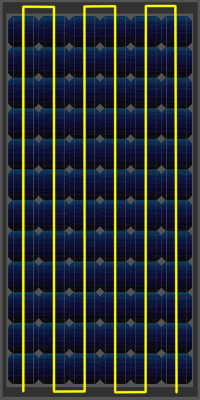
\includegraphics[width=40mm,height=80mm]{images/solar-facility/pvmodule-wiring.jpeg}
        };

        % Horizontal Measurement (Wires)
        % ==============================

        % Horizontal measurement between wires
        \draw (5mm,0mm) -- (5mm,4mm); % Vertical line
        \draw (11mm,0mm) -- (11mm,4mm);   % Vertical line

        % Measurement arrow
        \draw[-latex] (4mm,2mm) -- (5mm,2mm);
        \draw[-] (4mm,2mm) -- (31.5mm,2mm);
        \draw[latex-] (11mm,2mm) -- (12mm,2mm);

        % Measurment
        \node[anchor=west] at (12mm,3.75mm) {\small$d = \SI{127}{\milli\meter}$};


        % Vertical measurement (Wires)
        % ============================
        \draw (4mm,-1.5mm) -- (-4mm,-1.5mm); % horizontal line
        \draw (4mm,-78.5mm) -- (-4mm,-78.5mm); % horizontal line

        \draw[latex-latex] (-2mm,-1.5mm) -- (-2mm,-78.5mm); % measurement line

        % Measurement
        \node[rotate=90] at (-3.75mm,-38.5mm) {\small$l = \SI{1550}{\milli\meter}$};

        \node at (5mm,-82.5mm) {\small 1};
        \node at (11mm,-82.5mm) {\small 2};
        \node at (17mm,-82.5mm) {\small 3};
        \node at (23mm,-82.5mm) {\small 3};
        \node at (29mm,-82.5mm) {\small 2};
        \node at (35.5mm,-82.5mm) {\small 1};
    \end{scope}
\end{tikzpicture}


    \caption[PV-Modul, Modell f\"ur den Strompfad]{
        Solarmodul  gem\"ass Abbildung  \ref{fig:pvmodule} mit  Stromleitungen
        und  L\"angen   zur  Verbindung   der  Zellen. Die   Nummerierung  der
        Leiterbahnen   entspricht    der   Nummerierung    der   Koeffizienten
        in   Gleichungen   \ref{eq:rosa:a1}    bis   \ref{eq:rosa:a3}   (Seite
        \pageref{eq:rosa:a1}).%
    }
    \label{fig:pvmodule:wiring}
    \vspace*{-3em}
\end{wrapfigure}

Der  Pfad, den  der Strom  in  einem Modul  zur\"ucklegt, kann  je nach  Modul
mehrere Meter L\"ange  erreichen.  Dieser Effekt wird in  unserem Modell durch
eine Stromleitung modelliert, die \"uber  alle Zellen geht. In Realit\"at sind
die Leiter, welche die Zellen miteinander verbinden, ziemlich kurz (angenommen
die Zellen werden  von Kante zu Kante verbunden), aber  da der Strompfad durch
die ganze Zelle geht, wird der gesamte Strompfad in unserem Modell vereinfacht
als eine lange Leitung modelliert.

Zwischen   diesen   parallelen    Leiterbahnen   ergeben   sich   parasit\"are
Induktivit\"aten, die  im Folgenden  bestimmt und  in unser  Modell integriert
werden.  Die  angenommene Form und  die Abmessungen der  internen Stromleitung
sind  in  Abbildung   \ref{fig:pvmodule:wiring}  dargestellt. Die  Abmessungen
basieren auf folgenden Annahmen:

\begin{itemize}
    \tightlist
    \item
        Kantenl\"ange einer Zelle: \SI{125}{\milli\meter}
    \item
        Abstand zwischen zwei Modulen: \SI{2}{\milli\meter}
    \item
        \"Uberhang      am      oberen      und     unteren      Ende      des
        Moduls: \SI{14}{\milli\meter}
    \item
        Der Abstand  $d$ zweier Leiterbahnen ist  somit \SI{127}{\milli\meter}
        und
    \item
        die    L\"ange    $l$    einer   Leiterbahn    summiert    sich    auf
        \SI{1550}{\milli\meter}.
\end{itemize}


Zur  Berechnung  der  parasit\"aren  Induktivit\"at wird  \emph{The  Self  and
Mutual  Inductances  of Linear  Conductors}  von  Edward B. Rosa  herangezogen
\cite{ref:inductance:rosa}. Darin  wird   unter  anderem   die  Induktivit\"at
einer   Leiterkonfiguration  wie   sie  in   unserem  Modul   angenommen  wird
(Abbildung  \ref{fig:pvmodule:wiring}) bestimmt. Die  zugeh\"orige Formel  ist
in  Gleichung  \ref{eq:rosa:snake}  gegeben\footnotemark.
\footnotetext{%
    Die  Formeln  in   \cite{ref:inductance:rosa}  sind  im  \emph{CKG}-System
    (Centimeter,    Kilogramm,    Sekunden)     notiert,    f\"ur    Gleichung
    \ref{eq:rosa:snake} ist die Gleichung von  Rosa auf das SI-System normiert
    worden.%
}

\noindent Der  Wert f\"ur die Selbstinduktivit\"at  der verschiedenen Dr\"ahte
ist nicht  identisch; dies wird im  Summand $A_{\mathrm{i}}$ ber\"ucksichtigt,
der abh\"angt von der Anzahl  paralleler Leiterbahnen und ihrer Lage innerhalb
der  Leiteranordnung. F\"ur \num{6}  parallele Leiterbahnen  ergeben sich  die
Werte aus Gleichungen \ref{eq:rosa:a1}, \ref{eq:rosa:a2} und \ref{eq:rosa:a3}.


\begin{alignat}{2}
    \label{eq:rosa:snake}
    L &= \frac{\mu_{\mathrm{0}} \cdot l}{2 \cdot \pi}
    \cdot
    \left[
        \ln\left(
            \frac{d}{\rho}
        \right)
        + \frac{1}{4}
        - A_{\mathrm{i}}
    \right] & \quad \text{Selbstinduktivit\"at eines Leiters}
    \\
    \label{eq:rosa:a1}
    A_{\mathrm{1}} &= -\ln\left(\frac{15}{8}\right) & \text{\"ausserste Leiterbahnen} \\
    \label{eq:rosa:a2}
    A_{\mathrm{2}} &= \ln\left(\frac{16}{5}\right)  & \text{Leiterbahnen Nr. 2} \\
    \label{eq:rosa:a3}
    A_{\mathrm{3}} &= \ln\left(\frac{4}{3}\right)   & \text{Leiterbahnen Nr. 3, Mitte}
\end{alignat}

\begin{conditions}
    d              & Abstand zwischen zwei Leiterbahnen \\
    \rho           & Radius des Leiters \\
    A_{\mathrm{i}} & Korrektursummand f\"ur Leiterposition gem\"ass Abbildung \ref{fig:pvmodule:wiring} \\
\end{conditions}

Somit kann f\"ur  jeden Teil der Leitung in einem  Modul dessen Induktivit\"at
berechnet  werden. Diese  werden  anschliessend summiert  (Serieschaltung  von
Induktivit\"aten) und  als Gesamtinduktivit\"at  eines Moduls in  unser Modell
integriert.

Es   wird  von   einem   Leiterquerschnitt  von   \SI{4}{\milli\meter\squared}
ausgegangen,  was  einen   Leiterradius  $\rho$  von  \SI{1.128}{\milli\meter}
ergibt. Dies ist eine g\"angige Gr\"osse in PV-Installationen.

Die  Induktivit\"aten der  Leiterbahnen  innerhalb des  Moduls k\"onnen  somit
bestimmt werden:

\begin{alignat}{2}
    L_{\mathrm{1}} &= \frac{\mu_{\mathrm{0}} \cdot l}{2 \cdot \pi}
    \cdot
    \left[
        \ln\left(
            \frac{d}{\rho}
        \right)
        + \frac{1}{4}
        - A_{\mathrm{1}}
    \right]
    & = \SI{1.737}{\micro\henry} \\
    L_{\mathrm{2}} &= \frac{\mu_{\mathrm{0}} \cdot l}{2 \cdot \pi}
    \cdot
    \left[
        \ln\left(
            \frac{d}{\rho}
        \right)
        + \frac{1}{4}
        - A_{\mathrm{2}}
    \right]
    & = \SI{1.181}{\micro\henry} \\
    L_{\mathrm{3}} &= \frac{\mu_{\mathrm{0}} \cdot l}{2 \cdot \pi}
    \cdot
    \left[
        \ln\left(
            \frac{d}{\rho}
        \right)
        + \frac{1}{4}
        - A_{\mathrm{3}}
    \right]
    & = \SI{1.453}{\micro\henry}
\end{alignat}

\begin{conditions}
    \mu_{\mathrm{0}} = 4 \cdot \pi \cdot 10^{-7} & magnetische Permeabilit\"at des Vakuums \\
    l                = \SI{1550}{\milli\meter}   & L\"ange einer Leiterbahn                \\
    d                = \SI{127}{\milli\meter}    & Abstand zweier Leiterbahnen             \\
    \rho             = \SI{1.128}{\milli\meter}  & Radius des Leiters                      \\
    A_{\mathrm{1}}   =  -0.6286                  & Korrektursummand                        \\
    A_{\mathrm{2}}   =   1.1632                  & Korrektursummand                        \\
    A_{\mathrm{3}}   =   0.2877                  & Korrektursummand                        \\
\end{conditions}

\clearpage
Die Gesamtinduktivit\"at der Leiterbahnen in einem Modul ist somit:

\begin{equation}
    \label{eq:pvmodule:totalInductance}
    \underline{\underline{L_{\mathrm{Modul}}
    =
    2 \cdot \left(
        L_{\mathrm{1}} + L_{\mathrm{2}} + L_{\mathrm{3}}
    \right)
    = \SI{8.74}{\micro\henry}}}
\end{equation}

Es bleibt noch der Ohm'sche Widerstand der Leiterbahn zu bestimmen\footnotemark.
Dieser errechnet sich zu:

\footnotetext{%
    Es  sei  an   dieser  Stelle  darauf  hingewiesen,  dass   der  im  Modell
    der  Solarzelle  vorkommende  Seriewiderstand $R_{\mathrm{S}}$  nicht  die
    Leiterbahnen modelliert, sondern thermische Verluste im Halbleitersubstrat
    \cite{pvcell:masmoudi}%
}

\begin{equation}
    \label{eq:resistance:ohm:module}
    \underline{\underline{R = \frac{\rho \cdot l}{A} = \SI{44.2}{\milli\ohm}}}
\end{equation}

\begin{conditions}
    A = \SI{4}{\milli\meter\squared} & Querschnittsfl\"ache des Leiters \\
    \rho = \SI{0.0178}{\ohm\milli\meter\squared\per\meter} & Spezifischer Widerstand Leitungskupfer \cite{ref:kuchling:rhoCu} \\
    l = (6 \cdot 1550 + 5 \cdot 127)\si{\milli\meter} = \SI{9.935}{\meter} & Gesamtl\"ange des Leiters in einem Modul \\
\end{conditions}

Mit  diesen Informationen  kann  das Schaltbild  f\"ur  ein PV-Modul  bestimmt
werden,  was  die  Schaltung  in  Abbildung  \ref{fig:circuit:72x1:simplified}
ergibt. Dieses  Modell  wird im  Folgenden  benutzt,  um eine  Solaranlage  zu
modellieren.

\begin{figure}[h!tb]
    \centering
    \def\POSxUp{0,3,6}
\def\POSxDown{1,4,7}
\def\POSy{0,1,3}
\begin{circuitikz}
    \foreach \x in \POSxUp{
        \foreach \y in \POSy {
            \draw
            (\x,\y) to[empty photodiode] (\x,\y+1)
            ;
        }
        \draw (\x,2.5) node[rotate=90] {\ldots};
        \draw (\x,4) -- (\x + 1,4);
    }

    \draw(2,2.5) node {$\times 9$};
    \draw(5,2.5) node {$\times 9$};

    \foreach \x in \POSxDown{
        \foreach \y in \POSy {
            \draw
            (\x,\y+1) to[empty photodiode] (\x,\y)
            ;
        }
        \draw (\x,2.5) node[rotate=90] {\ldots};
    }

    % Connecting Lines between Strings
    \draw (1,0) -- (3,0);
    \draw (4,0) -- (6,0);

    % Series Inductance
    \draw (0,-2.5) to[L,l_=L] (0,0);

    % Series Resistance
    \draw (7,-2.5) to[R,l_=R] (7,0);

    % Connection Pins
    \draw (0,-2.5) -- (0,-3.5) node[ocirc] {~~IN};
    \draw (7,-2.5) -- (7,-3.5) node[ocirc] {~~OUT};

    % Bypass Diode
    \draw (0,-2.5) to[empty diode,*-*,l^={\footnotesize Freilaufdiode}] (7,-2.5);
\end{circuitikz}

    \caption[Ersatzschaltbild PV-Modul]{%
        Ersatzschaltbild   f\"ur  das   PV-Modul. Es   besteht  einem   Strang
        mit   72    Zellen   in   Serie   geschaltet    und   angeordnet   wie
        auf   dem   Modul   in    Abbildung   \ref{fig:pvmodule}   auf   Seite
        \pageref{fig:pvmodule}.     Zus\"atzlich    ist    die    parasit\"are
        Induktivit\"at  der Leiterbahnen  im Modul  ber\"ucksichtigt und  eine
        Freilaufdiode integriert.  Die vollst\"andige \code{LTspice}-Schaltung
        ist   in   Abbildung   \ref{fig:ltspice:jacModule:Diode}   auf   Seite
        \pageref{fig:ltspice:jacModule:Diode} dargestellt.%
    }
    \label{fig:circuit:72x1:simplified}
\end{figure}



% ---------------------------------------------------------------------------- %
\section{Modellierung eines Modulstrangs}
\label{sec:simu:model:module:string}
% ---------------------------------------------------------------------------- %

Der zu  simulierende Modulstrang soll  aus 20  Modulen bestehen, die  in Serie
miteinander  verbunden werden. Die  Induktivit\"at der  Leitungen, welche  die
Module  miteinander verbinden,  wird  vernachl\"assigt,  da die  zugeh\"origen
Distanzen  zwischen den  Leitern viel  gr\"osser sind,  als die  Distanzen der
Leiterbahnen innerhalb eines Moduls (siehe vorheriger Abschnitt).

Es  soll  jedoch  die  Induktivit\"at  der  Anschlussleitung  ber\"ucksichtigt
werden. Dabei   soll  von   einem   \SI{20}{\meter}  langen   Doppelleiterpaar
ausgegangen  werden, das  in einem  Abstand von  \SI{20}{\milli\meter} verlegt
worden ist. Dies ist nat\"urlich eine  idealisierte Annahme; in der Realit\"at
sind  diese Leiter  weder mit  konstant gleichem  Abstand noch  perfekt gerade
verlegt.

Die  von   Rosa  in  \cite{ref:inductance:rosa}  gegebene   Formel  f\"ur  die
Induktivit\"at eines geraden, parallelen Leiterpaares lautet\footnotemark:

\footnotetext{%
    Auch  hier  ist  Rosa's  Formel  auf  das  moderne  SI-System  konvertiert
    worden. Zudem wird  davon ausgegangen,  dass die  Leiter aus  Kupfer sind.
    Dessen  relative  Permeabilit\"at  $\mu_{\mathrm{r}}$  liegt  bei  etwa  1
    \cite{ref:kuchling:muRCu} und kann somit in der Gleichung vernachl\"assigt
    werden.

    Auch Kuchling gibt in \cite{ref:Kuchling:Ltwo} die gleiche Formel.%
}

\begin{equation}
    \label{eq:rosa:dualwire}
    \underline{\underline{L = \frac{\mu_{0}}{\pi} \cdot \left[ \ln\left(\frac{d}{\rho}\right) + \frac{1}{4} \right]
    = \SI{25}{\micro\henry}}}
\end{equation}

\begin{conditions}
    \mu_{\mathrm{0}} = 4 \cdot \pi \cdot 10^{-7} & magnetische Permeabilit\"at des Vakuums \\
    l                = \SI{20}{\meter}           & L\"ange des Leiterpaares (ein Weg)    \\
    d                = \SI{20}{\milli\meter}     & Abstand der Leiter                    \\
    \rho             = \SI{1.128}{\milli\meter}  & Radius des Leiters                    \\
\end{conditions}

Da zwei parallel  verlaufende Leiter im Prinzip  einen Kondensator darstellen,
soll  an  dieser  Stelle  auch   die  parasit\"are  Kapazit\"at  der  zu-  und
wegf\"uhrenden Leiterbahnen ber\"ucksichtigt werden. Die Formel zur Berechnung
dieser Kapazit\"at ist gem\"ass Kuchling \cite{ref:Kuchling:CTwo}:

\begin{equation}
    \label{eq:rosa:dualwire}
    \underline{\underline{C = \frac{\pi \cdot \epsilon_{0} \cdot \epsilon_{\mathrm{r}} \cdot l}{\ln\left(\frac{d}{\rho}\right)}
    = \SI{193.5}{\pico\farad}}}
\end{equation}

\begin{conditions}
    \epsilon_{0} = \SI{8.854}{\pico\farad\per\meter} & Elektrische Feldkonstante          \\
    \epsilon_{\mathrm{r}} = 1                        & Permittivit\"atszahl von Luft      \\
    l                = \SI{20}{\meter}               & L\"ange des Leiterpaares (ein Weg) \\
    d                = \SI{20}{\milli\meter}         & Abstand der Leiter                 \\
    \rho             = \SI{1.128}{\milli\meter}      & Radius des Leiters                 \\
\end{conditions}

\clearpage
Der Ohm'sche Widerstand der Anschlussleitung errechnet sich zu:

\begin{equation}
    \label{eq:resistance:ohm:module}
    \underline{\underline{R = \frac{\rho \cdot l}{A} = \SI{178}{\milli\ohm}}}
\end{equation}

\begin{conditions}
    A    = \SI{4}{\milli\meter\squared} & Querschnittsfl\"ache des Leiters \\
    \rho = \SI{0.0178}{\ohm\milli\meter\squared\per\meter} & Spezifischer Widerstand Leitungskupfer \cite{ref:kuchling:rhoCu} \\
    l    = \SI{40}{\meter} & Gesamtl\"ange der Anschlussleitung (beide Wege) \\
\end{conditions}

\vspace*{3em}
\begin{figure}[h!tb]
    \centering
    \def\POSx{9,8,7,6,5,4,3,2,1,0}
%\def\POSxRight{2,3,4,5,6,7,8,9,10,11}
\begin{circuitikz}
    %(12,0) -- (10,0)

    % Right to Left
    \foreach \x in \POSx {
        \draw
        (\x,1.5) to[empty photodiode] (\x - 1,1.5)
        ;
    }

    % Left to Right
    \foreach \x in \POSx {
        \draw
        (\x-1,-1.5) to[empty photodiode] (\x,-1.5)
        ;
    }

    % Endpoints
    \draw (-1,1.5) -- (-1,-1.5);

    % Stuff on the right
    \draw (9,1.5)  -- (9,0.75)  to[L,l^=L] (12,0.75)  node[ocirc] { };
    \draw (9,-1.5) -- (9,-0.75) to[R,l_=R] (12,-0.75) node[ocirc] { };
    \draw (9.5,0.75) node[circ] { } to[C,l^=C] (9.5,-0.75) node[circ] { };
\end{circuitikz}

    \caption[Ersatzschaltbild Modulstrang mit Verbindungsleitung]{
        Modell  eines Modulstrangs  aus  20 seriell  geschalteten Modulen  mit
        Ber\"ucksichtigung der Resistivit\"at,  Induktivit\"at und Kapazit\"at
        einer \SI{20}{\meter} langen Zuleitung%
    }
    \label{fig:pvstring}
\end{figure}

\vspace*{3em}
Abbildung  \ref{fig:pvstring} zeigt  das  Ersatzschaltbild eines  Modulstrangs
aus    20   in    Serie   geschalteten    Modulen   mit    den   parasit\"aren
Leiterimpedanzen. Dieses  und  die  vorangegangenen   Modelle  werden  nun  in
\code{LTspice} implementiert und f\"ur Simulationen benutzt.

% **************************************************************************** %
\chapter{L\"osungsans\"atze und Simulationen}
\label{chap:simu}
% **************************************************************************** %


Mit   den  im   vorigen  Kapitel   entwickelten  Modellen   werden  nun   drei
L\"osungsans\"atze auf  ihre Vor-  und Nachteile untersucht,  um anschliessend
eine Variante auszuw\"ahlen. Zuerst wird die  Einkopplung eines Signals in die
DC-Leitung mittels induktiver Kopplung untersucht, gefolgt von der kapazitiven
Einkopplung.   Zuletzt  wird  die  Machbarkeit  der  OOK  mittels  Kurzschluss
beurteilt. Eine zusammenfassende Gegen\"uberstellung der Simulationsergebnisse
befindet sich auf Seite \pageref{subsec:simu:conclusion}.

Zur  Simulation wird  \code{LTspice  IV}  \cite{ref:ltspice} von  \emph{Linear
Technologies} verwendet. Es  ist zu jeder  \code{LTspice}-Schaltung angegeben,
wo die  zugeh\"orige Datei  auf dem Datentr\"ager  gespeichert ist,  falls der
geneigte Leser selbst simulieren m\"ochte.


% ---------------------------------------------------------------------------- %
\section{Induktive Einkopplung}
\label{sec:simu:coupling:inductive}
% ---------------------------------------------------------------------------- %

Bei der induktiven Einkopplung wird eine  Spule um die DC-Leitung gelegt.  Auf
diese  Spule  wird  vom  Sensor  das  zu  \"ubertragende  Signal  gegeben  und
die  Spule induziert  in  der DC-Leitung  entsprechende Spannungs-Rippel,  die
vom  \Master~ausgewertet werden  k\"onnen. Der  entsprechende Schaltkreis  ist
schematisch in Abbildung \ref{fig:circuit:coupling:inductive} dargestellt.

\code{LTspice} modelliert diese  Situation als gekoppelte Spulen  mit je einer
Induktivit\"at (L1  und L2 in  Abbildung \ref{fig:circuit:coupling:inductive})
und einem Kopplungsfaktor K. Es gilt, diese drei Parameter zu bestimmen.

Wir  werden   f\"ur  unsere   Simulationen  von  einer   Toroidspule  gem\"ass
Abbildung  \ref{fig:toroid:geometry}  mit   20  Prim\"arwicklungen  und  einer
Sekund\"arwindung (der DC-Leitung) ausgehen.  Die relative Permeabilit\"at von
ferromagnetischen Materialien  kann enorm  stark variieren; Werte  von einigen
Dutzend bis zu  mehreren Tausend k\"onnen auftreten. Wir  werden f\"ur unseren
Kern eine Permeabilit\"atszahl $\mu_{\mathrm{r}} = 400$ annehmen.

\clearpage
\begin{figure}[h!tb]
    \centering
    \begin{circuitikz}
    \draw
    (-1,0) to[empty photodiode,o-,l_=PV-Modul] (1,0) -- (2,0) to[L,l_=L2] (4,0) -- (7,0) to[L,l_=L2] (9,0) to[short] (10,0)
    (2.5,0.30) -- (3.5,0.30)
    (2.25,0.35) node {K}
    (2.5,0.40) -- (3.5,0.40)
    (7.5,0.30) -- (8.5,0.30)
    (7.25,0.35) node {K}
    (7.5,0.40) -- (8.5,0.40)
    (4,2) -- (4,0.7) to[L,l_=L1] (2,0.7) -- (2,2) to[sinusoidal voltage source,l^=$U_{\mathrm{Sender}}$] (4,2)
    (9,2) -- (9,0.7) to[L,l_=L1] (7,0.7) -- (7,2) to[sinusoidal voltage source,l^=$U_{\mathrm{Empf\text{\"a}nger}}$] (9,2)
    ;
\end{circuitikz}

    \caption[Prinzip der induktiven Einkopplung]{Induktive Einkopplung}
    \label{fig:circuit:coupling:inductive}
\end{figure}


Die Selbstinduktivit\"at unserer Toroidspule errechnet sich somit zu:

\begin{equation}
    \label{eq:selfInductance:toroid:primary}
    L_{\mathrm{1}} = \frac{\mu_{0} \mu_{\mathrm{r}} r^2 N_1^2}{2 R} \approx \underline{\underline{\SI{200}{\micro\henry}}}
\end{equation}

%\begin{figure}[h!tb]
\marginpar{%
    \begin{tikzpicture}
    \footnotesize
    \begin{scope}[x={(0mm,0.9\textwidth)},y={(0mm,30mm)}]
        \draw (0mm,0mm) circle[radius = 6mm];
        \draw (0mm,0mm) circle[radius = 10mm];
        \draw[dashed] (0mm,0mm) circle[radius = 8mm];
        \draw[|-latex] (0mm,0mm) -- (8mm,0mm);
        \draw (3.5mm,2mm) node {R};
        \draw[-latex] (-14mm,0mm) -- (-10mm,0mm);
        \draw (-12mm,2mm) node {2r};
        \draw (-10mm,0mm) -- (-6mm,0mm);
        \draw[latex-] (-6mm,0mm) -- (-4mm,0mm);
    \end{scope}
\end{tikzpicture}

    \figcaption[Geometrie Kopplungsspule]{\protect\raggedright Geometrie der Spule}
    \label{fig:toroid:geometry}%
}
%\end{figure}

\begin{conditions}
    \mu_0 = 4 \cdot \pi \cdot 10^{-7} & magnetische Permeabilit\"at des Vakuums               \\
    \mu_{\mathrm{r}} = 400 & angenommene relative magnetische Permeabilit\"at des Kerns       \\
    r = \SI{4}{\milli\meter} & Radius des Kernquerschnitts (Abb. \ref{fig:toroid:geometry})  \\
    R = \SI{8}{\milli\meter} & mittlerer Radius des Toroids (Abb. \ref{fig:toroid:geometry}) \\
    N_1 = 20 & Anzahl Windungen \\
\end{conditions}

Die Induktivit\"at der sekund\"aren Seite lautet:

\begin{equation}
    \label{eq:selfInductance:toroid:secondary}
    L_{\mathrm{2}} = L_{1} \cdot \frac{N_2^2 }{N_1^2} \approx \underline{\underline{\SI{500}{\nano\henry}}}
\end{equation}

\begin{conditions}
    L_{\mathrm{1}} = \SI{200}{\micro\henry}
    & Selbstinduktivit\"at der Prim\"arseite (Gl. \ref{eq:selfInductance:toroid:primary})\\

    N_1 = 20 & Windungsn Prim\"arseite (Transmitter/Receiver) \\
    N_2 = 1  & Windungen Sekund\"arseite (DC-Leitung) \\
\end{conditions}

Der Kopplungsfaktor beschreibt, wie gross  der Anteil des magnetischen Flusses
ist, welcher beide Spulen durchfliesst. Ein Kopplungsfaktor von null bedeutet,
dass die  beiden Spulen  v\"ollig entkoppelt sind,  ein Kopplungsfaktor  von 1
heisst, dass der gesamte Fluss, welcher  die eine Spule durchfliesst, auch die
andere Spule durchfliesst.  Es wird  hier ein Streuverlust von 5\% angenommen,
was einen Kopplungsfaktor von 0.95 ergibt.

\clearpage
Es  wird   zuerst  eine  vereinfachte  Schaltung   untersucht,  bestehend  aus
einem  Modul,  dem  Sender  und  dem  Empf\"anger,  dargestellt  in  Abbildung
\ref{fig:ltspice:inductive:singleModule}.

Abbildung   \ref{fig:simu:inductive:singleModule}   zeigt  den   zugeh\"origen
Spannungsverlauf am Empf\"anger.   Das Signal kommt sauber an,  ist aber nicht
sehr stark.

\begin{figure}[h!tb]
    \centering
    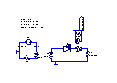
\includegraphics[width=0.67\textwidth]{images/ltspice/jac/inductive-singleModule.eps}
    \caption[Induktive Einkopplung, vereinfachte \code{LTspice}-Schaltung]{%
        \code{LTspice}-Schaltung f\"ur den vereinfachten Schaltkreis zur
        Simulation der induktiven Einkopplung\protect\\
        Dateipfad: \code{ltspice/inductive/singleModule.asc}%
    }
    \label{fig:ltspice:inductive:singleModule}
\end{figure}

\begin{figure}[h!tb]
    \begin{tikzpicture}
    %\begin{scope}[x={(0mm,0mm)},y={(175mm,\textwidth)}] % for four plots
    \begin{scope}[x={(0mm,0.95\textwidth)},y={(0mm,50mm)}]
        \begin{axis}[%
                title=Spannung am Empf\"anger,
                %title=$R_{\mathrm{Last}}$
                height=50mm,
                width=0.95\textwidth,
                at={(0,0)},
                grid=both,
                xlabel=Zeit (\si{\micro\second}),
                ylabel=Spannung (\si{\milli\volt}),
                change x base=true,
                change y base=true,
                x SI prefix=micro,
                y SI prefix=milli,
                xmin = 0,
                xmax = 10e-6,
                %legend cell align = left,
                %legend style={at={(125mm,-10mm)},anchor=north east},
           ]
           \addplot[-,blue] table[x = time,y = V(receiver)] {data/inductive/inductive-singleModule.dat};
        \end{axis}
   \end{scope}
\end{tikzpicture}

    \caption[Simulationsergebniss induktive Einkopplung, vereinfachte Schaltung]{%
        Simulationsergebniss f\"ur die Spannung am Empf\"anger aus Abbildung
        \ref{fig:ltspice:inductive:singleModule}%
    }
    \label{fig:simu:inductive:singleModule}
\end{figure}

\clearpage
Zur  Simulation eines  ganzen Modulstrangs  wird die  Schaltung aus  Abbildung
\ref{fig:ltspice:inductive:complete}  benutzt; der  Modulstrang basiert  dabei
auf den Herleitungen aus Abschnitt \ref{sec:simu:model:module:string} ab Seite
\pageref{sec:simu:model:module:string}.

Abbildung  \ref{fig:simu:inductive:stepping}  enth\"alt  Simulationsergebnisse
f\"ur    verschiedene   Lastimpedanzen    bei    einer   Senderfrequenz    von
\SI{1}{\mega\hertz}.   Die zugeh\"origen Impedanzkombinationen sind in Tabelle
\ref{tab:inductive:stepping:params}  aufgelistet. Simulationen  mit  h\"oheren
resistiven  Anteilen w\"aren  interessant, allerdings  hat \code{LTspice}  bei
weiterem  Ansteigen von  \code{Rload} (vermutlich  numerische) Schwierigkeiten
und  die Simulationszeit  steigt auf  Tage bis  Wochen (falls  sie \"uberhaupt
jemals endet und  die Software nicht in einem Kreis  von nicht konvergierenden
Bedingungen festh\"angt).

Es  ist zu  erkennen, dass  das Signal  am Empf\"anger  nicht besonders  stark
von der  Lastimpedanz abh\"angt. Allerdings  ist die  Signalamplitude ziemlich
klein und  betr\"agt nur  einige Millivolt. Daf\"ur ist  das Signal  in seiner
Form  nur sehr  schwach  verzerrt,  was wir  als  einen  sehr positiven  Punkt
bewerten. Vorausgesetzt,  das  Signal  wird  nicht  von  St\"orungen  auf  der
Leitungen \"uberdeckt, w\"urde  es sich gut f\"ur  Filterung und Verst\"arkung
eignen. Ob  dies  wirklich  der  Fall  ist, kann  im  Rahmen  dieses  Projekts
allerdings  nicht  eruiert  werden,  da wir  weder  einen  gen\"ugend  grossen
Modulstrang  noch die  zur gr\"undlichen  Untersuchung erforderliche  Zeit zur
Verf\"ugung haben. Soll  das System  aber wirklich in  der Praxis  zum Einsatz
kommen, muss dieser Punkt sicherlich genauer untersucht werden.

\begin{figure}[h!tb]
    \centering
    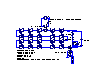
\includegraphics[width=0.95\textwidth]{images/ltspice/jac/inductive.eps}
    \caption[Induktive Einkopplung, \code{LTspice}-Schaltung f\"ur Modulstrang]{%
        Schaltung  zur   Simulation  eines  Modulstranges   mit  parasit\"aren
        Impedanzen in der Zuleitung und komplexer Lastimpedanz.\protect\\
        Dateipfad: \code{ltspice/inductive/string.asc}%
    }
    \label{fig:ltspice:inductive:complete}
\end{figure}

\begin{figure}[h!tb]
    \begin{tikzpicture}
    %\begin{scope}[x={(0mm,0mm)},y={(175mm,\textwidth)}] % for four plots
    \begin{scope}[x={(0mm,0.95\textwidth)},y={(0mm,50mm)}]
        \begin{axis}[%
                title=Spannung am Empf\"anger{,} variierende Lastimpedanzen,
                height=50mm,
                width=0.95\textwidth,
                at={(0,0)},
                grid=both,
                xlabel=Zeit (\si{\micro\second}),
                ylabel=Spannung (\si{\milli\volt}),
                change x base=true,
                change y base=true,
                x SI prefix=micro,
                y SI prefix=milli,
                xmin = 0,
                xmax = 10e-6,
           ]
           \addplot[-,blue] table[x = time,y = V(receiver)] {data/inductive/inductive-CloadRload-stepped.dat};
        \end{axis}
   \end{scope}
\end{tikzpicture}

    \caption[Simulationsergebniss, induktive Einkopplung, Modulstrang]{%
        Simulationsergebniss f\"ur  die Spannung am Empf\"anger  aus Abbildung
        \ref{fig:ltspice:inductive:complete}  mit den  Parametern aus  Tabelle
        \ref{tab:inductive:stepping:params}%
    }
    \label{fig:simu:inductive:stepping}
\end{figure}
\vspace*{-1em}

\begin{table}[h!tb]
    \centering
    \caption{%
        Lastimpedanzparameter  f\"ur die  Simulationsergebnisse aus  Abbildung
        \ref{fig:simu:inductive:stepping}
    }
    \small
    \label{tab:inductive:stepping:params}
    \begin{tabular}{rr|rr|rr}
        \toprule
        \code{Cload}             & \code{Rload} & \code{Cload}             & \code{Rload}  & \code{Cload}             & \code{Rload} \\
        \midrule
        \SI{  1}{\nano\farad}    & \SI{1}{\ohm} & \SI{  1}{\nano\farad}    & \SI{10}{\ohm} & \SI{  1}{\nano\farad}    & \SI{50}{\ohm} \\
        \SI{ 10}{\nano\farad}    & \SI{1}{\ohm} & \SI{ 10}{\nano\farad}    & \SI{10}{\ohm} & \SI{ 10}{\nano\farad}    & \SI{50}{\ohm} \\
        \SI{100}{\nano\farad}    & \SI{1}{\ohm} & \SI{100}{\nano\farad}    & \SI{10}{\ohm} & \SI{100}{\nano\farad}    & \SI{50}{\ohm} \\
        \SI{  1}{\micro\farad}   & \SI{1}{\ohm} & \SI{  1}{\micro\farad}   & \SI{10}{\ohm} & \SI{  1}{\micro\farad}   & \SI{50}{\ohm} \\
        \SI{ 10}{\micro\farad}   & \SI{1}{\ohm} & \SI{ 10}{\micro\farad}   & \SI{10}{\ohm} & \SI{ 10}{\micro\farad}   & \SI{50}{\ohm} \\
        \SI{100}{\micro\farad}   & \SI{1}{\ohm} & \SI{100}{\micro\farad}   & \SI{10}{\ohm} & \SI{100}{\micro\farad}   & \SI{50}{\ohm} \\
        \bottomrule
    \end{tabular}
\end{table}

\clearpage
Interessant    ist    der    Betrieb    des    Senders    mit    Eigenfrequenz
(ca. \SI{240}{\kilo\hertz} in diesem  Fall) des Modulstrangs\footnotemark. Der
zugeh\"orige    Spannungsverlauf    am    Empf\"anger   ist    in    Abbildung
\ref{fig:simu:inductive:resonance}   abgebildet. Hier    wird   ein   vielfach
gr\"osserer  Signalpegel  erreicht;  allerdings  ben\"otigt  das  Signal  etwa
\SI{100}{\micro\second},  bis  es wirklich  seine maximale  Amplitude erreicht
hat. Da  bei  diesem System  jedoch  keine  sehr hohen  Datenraten  ben\"otigt
werden, muss dies nicht unbedingt kritisch sein.

\footnotetext{%
    Die Eigenfrequenz  ist hier nicht  mathematisch bestimmt, sondern  aus den
    Simulationen abgelesen worden.%
}

\begin{figure}[h!tb]
    \begin{tikzpicture}
    %\begin{scope}[x={(0mm,0mm)},y={(175mm,\textwidth)}] % for four plots
    \begin{scope}[x={(0mm,0.95\textwidth)},y={(0mm,50mm)}]
        \begin{axis}[%
                title=Spannung am Empf\"anger bei Eigenfrequenz,
                height=50mm,
                width=0.95\textwidth,
                at={(0,0)},
                grid=both,
                xlabel=Zeit (\si{\micro\second}),
                ylabel=Spannung (\si{\milli\volt}),
                change x base=true,
                change y base=true,
                x SI prefix=micro,
                y SI prefix=milli,
                xmin = 0,
                xmax = 120e-6,
           ]
           \addplot[-,blue] table[x = time,y = V(receiver)] {data/inductive/inductive-resonance.dat};
        \end{axis}
   \end{scope}
\end{tikzpicture}

    \caption[Simulationsergebniss induktive Einkopplung bei Resonanz]{%
        Simulationsergebniss f\"ur die Spannung am Empf\"anger aus Abbildung
        \ref{fig:ltspice:inductive:complete}%
    }
    \label{fig:simu:inductive:resonance}
\end{figure}


Abschliessend kann man  zur induktiven Kopplung sagen, dass  sie bei kleineren
Aufbauten  gut  funktionieren  sollte,   dass  aber  bei  gr\"osseren  Anlagen
m\"oglicherweise  zus\"atzliche  Massnahmen  n\"otig sein  k\"onnten,  um  das
Signal klar empfangen und auswerten  zu k\"onnen. Dies k\"onnte z.B. bedeuten,
dass  unser System  die Eigenfrequenz  des Modulstrangs  selbst ausmisst   und
sich entsprechend  selbst konfiguriert,  um stets  auf der  optimalen Frequenz
\"ubermitteln zu k\"onnen.

Das in den \code{LTspice}-Schaltungen verwendete Symbol f\"ur ein PV-Modul ist
im Anhang auf Seite \pageref{fig:ltspice:module:symbol} erkl\"art.

% ---------------------------------------------------------------------------- %
\clearpage
\section{Kapazitive Einkopplung}
\label{sec:simu:coupling:capacitive}
% ---------------------------------------------------------------------------- %

Bei der  kapazitiven Einkopplung  wird eine  Signalquelle via  Kondensator mit
der  DC-Leitung  verbunden. Bei  jedem  Modul und  am  Ende  des  Modulstrangs
ist   dabei  eine   Einkopplung   vorgesehen. Das   Prinzip  ist   schematisch
in   Abbildung   \ref{fig:circ:coupling:capacitive}   dargestellt. F\"ur   die
nachfolgenden  Versuche  wird  eine Tr\"agerfrequenz  von  \SI{1}{\mega\hertz}
angenommen, sofern nicht anders angegeben.

Sowohl \Master ~wie auch \Sensor~ k\"onnen dabei Signale senden und empfangen;
das Verfahren ist bidirektional.

\begin{figure}[h!tb]
    \centering
    \begin{circuitikz}
    \draw
    (0,0) to[empty photodiode,o-,l_=PV-Modul] (1,0) to[short] (10,0) node[ocirc] { }

    (3,0) node[circ] { } to[C,l^=Kopplung] (3,-1.5) to[sinusoidal voltage source,l^=$U_{\mathrm{Sender}}$] (3,-3) node[sground] { }

    (9,0) node[circ] { } to[C,l^=Kopplung] (9,-1.5) -- (9,-3) node[ocirc] {~~$U_{\mathrm{Receiver}}$};
    ;
\end{circuitikz}

    \caption[Ersatzschaltbild kapazitive Einkopplung]{%
        Vereinfachte Darstellung  der kapazitiven  Einkopplung mit  Sender auf
        der linken  Seite und  Empf\"anger auf der  rechten Seite. Prinzipiell
        ist das Verfahren jedoch bidirektional.%
    }
    \label{fig:circ:coupling:capacitive}
\end{figure}

Zur   Simulation   in  \code{LTspice}   wird   die   Schaltung  in   Abbildung
\ref{fig:ltspice:capacitive:string} benutzt. Sie basiert  auf dem Modell eines
Modulstrangs von Abbildung  \ref{fig:pvstring} (Seite \pageref{fig:pvstring}),
erg\"anzt  um  die  Ein-  und  Auskopplungsschaltung. Zus\"atzlich  wurde  eine
komplexe Lastimpedanz eingebaut.

Es   werden   der   Signalpegel   am  Empf\"anger   bei   zwei   verschiedenen
Senderpositionen  untersucht: Eine zu  Beginn des  Strangs, eine  am Ende  des
Strangs. Ist der  Sender am Anfang  des Strangs positioniert, muss  das Signal
durch alle restlichen Module, um an den Empf\"anger zu gelangen; es sind dabei
Verzerrungen und Abschw\"achungen des Signals zu beobachten.


\begin{figure}[h!tb]
    \centering
    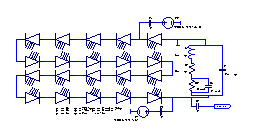
\includegraphics[width=0.75\textwidth]{images/ltspice/jac/capacitive.eps}
    \caption
    [\code{LTspice}-Schaltung kapazitive Einkopplung, Modulstrang]
    {%
        Simulationsschaltung     eines     Modulstrangs    mit     kapazitiver
        Einkopplung    eines    Signals.
        Die  Sender  werden  durch  Sinus-Spannungsquellen  simuliert. Es  ist
        jeweils  nur ein  Sender  aktiv  in der  Simulation,  der andere  wird
        abgeh\"angt.\protect\\
        Dateipfad: \code{ltspice/capacitive/string.asc}%
    }
    \label{fig:ltspice:capacitive:string}
\end{figure}

Die    in    \code{LTspice}    benutzte    Schaltung    ist    in    Abbildung
\ref{fig:ltspice:capacitive:string}      gezeigt.       Die      zugeh\"origen
Simulationsresultate   sind    in   Abbildung   \ref{fig:simu:capacitive:tran}
zu sehen.%

\begin{figure}[h!tb]
    \begin{tikzpicture}
    \begin{scope}[x={(0mm,0.95\textwidth)},y={(0mm,50mm)}]
        \begin{axis}[%
                title=Signalpegel am Empf\"anger,
                height=50mm,
                width=0.95\textwidth,
                at={(0,0)},
                grid=both,
                xlabel=Zeit (\si{\micro\second}),
                ylabel=Spannung (\si{\volt}),
                change x base=true,
                x SI prefix=micro,
                xmin = 0,
                xmax = 10e-6,
                legend cell align = left,
                legend style={at={(125mm,-10mm)},anchor=north east},
           ]
           \addplot[-,blue] table {data/capacitive/capacitive-stringStart.dat};
           \addplot[-,teal] table {data/capacitive/capacitive-stringEnd.dat};
           \legend{Sender am Anfang des Strangs,Sender am Ende des Strangs};
        \end{axis}
   \end{scope}
\end{tikzpicture}

    \caption[Simulationsergebnisse kapazitive Einkopplung, Modulstrang]{%
        Transientensimulation  der  kapazitiven   Einkopplung  am  Anfang  des
        Modulstrangs und  am Ende des  Modulstrangs. Ist der Sender  am Anfang
        des Strangs, wird das Signal merklich abgeschw\"acht und verzerrt.%
    }
    \label{fig:simu:capacitive:tran}
\end{figure}


% ---------------------------------------------------------------------------- %
\clearpage
\section{Signalcodierung mittels Kurzschluss}
\label{sec:simu:short}
% ---------------------------------------------------------------------------- %

Bei   dieser    L\"osungsvariante   wird    jeweils   ein    Modul   gesteuert
kurzgeschlossen. Dies  verursacht   (theoretisch)  kurze  Spannungseinbr\"uche
auf   der    DC-Leitung,   welche    vom   Empf\"anger    ausgewertet   werden
k\"onnen,   wie   in   Abbildung   \ref{fig:modulation:concepts}   auf   Seite
\pageref{fig:modulation:concepts} vereinfacht dargestellt.

Da die Spannungseinbr\"uche  auf der Leitung bei diesem  Verfahren sehr abrupt
sind,  k\"onnen  die im  System  vorhandenen  Induktivit\"aten gem\"ass  $v  =
L  \cdot  \frac{\mathrm{d}i}{\mathrm{d}t}$  (Spannung  in  Abh\"angigkeit  der
Strom\"anderung \"uber  einer Induktivit\"at) und der  Lenz'schen Regel diesen
abrupten \"Anderungen  Widerstand leisten. Wenn  diese Gegenspannung  zu gross
ist, kann es sein, dass das  Signal kompensiert wird und nicht mehr auswertbar
ist.

Es  werden  in   diesem  Abschnitt  zuerst  Sender   und  Empf\"anger  separat
untersucht; anschliessend wird das Gesamtsystem evaluiert.


% ---------------------------------------------------------------------------- %
\subsection{Sender}
\label{subsec:simu:ask:sensor}
% ---------------------------------------------------------------------------- %

Das  gesteuerte Kurzschliessen  des Moduls  wird mit  einem MOSFET  umgesetzt,
welcher zwischen  Eingang und  Ausgang des Moduls  durchschalten kann  und vom
Microcontroller auf dem Sensor gesteuert wird. \fref{fig:module:mosfet:simple}
zeigt diesen Aufbau schematisch.

\begin{wrapfigure}{r}{60mm}
    \vspace*{-1em}
    \centering
    % Pro memoriam:
%
%            |  D
%      | |---+
%      |
%      | |<--+  B
%      |     |
% G ---+ |---+
%            |  S
%(mos.B) node[anchor=west] {B}
%(mos.G) node[anchor=east] {G}
%(mos.D) node[anchor=north] {D}
%(mos.S) node[anchor=south] {S}

\begin{circuitikz}
    \small
    \draw
    (4.5,1) node[nigfete] (mos) {MOSFET}

    (0,0) to[empty photodiode,l_=PV-Modul] (0,2) -- (4.5,2) -- (mos.D)
    %(0,0) to[dcisource,l_=PV-Modul] (0,4) -- (8,4) -- (mos.D)
    (mos.S) -- (4.5,0) -- (0,0)

    (2.25,0.725) to[sinusoidal voltage source,l^=Controller] (mos.G)
    (2.25,0.725) -- (2.25,0) node[circ] { }
    ;
\end{circuitikz}

    \caption[Grundprinzip Kurzschluss mit Transistor]{%
        Gesteuerter     Kurzschluss     eines    Solarmoduls     mit     einem
        microcontroller-gesteuerten Transistor.%
    }
    \label{fig:module:mosfet:simple}
    \vspace*{-1.0em}
\end{wrapfigure}

Die  Ansteuerung des  Transistors  erfolgt mit  \SI{3.3}{\volt},  da dies  die
maximale Spannung  ist, welche der  auf dem Sensor  platzierte Microcontroller
ausgeben kann. Es muss  dabei beachtet werden, dass  der gew\"ahlte Transistor
vollst\"andig durchschaltet und in S\"attigung betrieben wird, damit der Strom
m\"oglichst ungehindert am kurzgeschlossenen Modul vorbeifliessen kann.

\begin{wrapfigure}{l}{65mm}
    \vspace*{-1em}
    \centering
    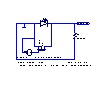
\includegraphics[width=65mm]{images/ltspice/jac/shortcircuit-transmitter.eps}
    \caption[\code{LTspice}-Schaltung Kurzschlussmethode, Sender, vereinfacht]{
        Simulationsschema  f\"ur  ein  einzelnes Modul  mit  kurzschliessendem
        Transistor und angeschlossener Last von \SI{1}{\kilo\ohm}.\protect\\
        Dateipfad: \code{ltspice/short/single.asc}%
    }
    \label{fig:ltspice:shortCircuit:transmitter}
    \vspace*{-2em}
\end{wrapfigure}

Ein  weiterer  kritischer  Punkt  ist,  dass die  im  Modul  (oder sonstwo  im
Stromkreis)  vorhandenen   Kapazit\"aten  zu  starken   Stromspitzen  f\"uhren
k\"onnen, welche den Transistor besch\"adigen k\"onnten.

Zuerst wird ein vereinfachtes Szenario simuliert: Ein einzelnes Modul mit einem
kurzschliessenden Transistor und einer Ohm'schen Last, dargestellt in Abbildung
\ref{fig:ltspice:shortCircuit:transmitter}.


\begin{figure}[h!tb]
    \begin{tikzpicture}
    \begin{scope}[x={(0mm,0.95\textwidth)},y={(0mm,150mm)}]
        \begin{axis}[%
            title=Spannung am Knoten \code{MEASURE},
            height=45mm,
            width=0.95\textwidth,
            at={(0,100mm)},
            grid=both,
            xlabel=Zeit (\si{\micro\second}),
            ylabel=Spannung (\si{\volt}),
            xmin = 0,
            xmax = 2e-4,
            change x base=true,
            x SI prefix=micro,
        ]
            \addplot[-,blue] table[x=time, y=V(measure)] {data/short-circuit/shortcircuit-transmitter-0.2ms.dat};
        \end{axis}
        \begin{axis}[%
            title=Strom durch MOSFET und Modul,
            height=45mm,
            width=0.95\textwidth,
            at={(0,50mm)},
            grid=both,
            xlabel=Zeit (\si{\micro\second}),
            ylabel=Strom (\si{\ampere}),
            xmin = 0,
            xmax = 2e-4,
            change x base=true,
            x SI prefix=micro,
        ]
            \addplot[-,blue] table[x=time, y=Id(MOS)] {data/short-circuit/shortcircuit-transmitter-0.2ms.dat};
            \addplot[-,magenta] table[x=time, y=I(module)] {data/short-circuit/shortcircuit-transmitter-0.2ms.dat};
            \legend{MOSFET,PV-Modul};
        \end{axis}
        \begin{axis}[%
            title=Leistung im MOSFET und PV-Modul,
            height=45mm,
            width=0.95\textwidth,
            at={(0,0)},
            grid=both,
            xlabel=Zeit (\si{\micro\second}),
            ylabel=Leistung (\si{\watt}),
            xmin = 0,
            xmax = 1.5e-6,
            change x base=true,
            x SI prefix=micro,
        ]
            \addplot[-,blue] table[x=time, y=powerMOS] {data/short-circuit/shortcircuit-transmitter-PPeak.dat};
            \addplot[-,magenta] table[x=time, y=powerModule] {data/short-circuit/shortcircuit-transmitter-PPeak.dat};
            \legend{MOSFET,PV-Modul};
        \end{axis}
   \end{scope}
\end{tikzpicture}

    \caption[Simulationsergebnisse Kurzschlussmethode, Sender]{%
        Transientensimulation    f\"ur     einen    gesteuerten    Kurzschluss
        \"uber     ein     Solarmodul     mit     einer     rein     Ohm'schen
        Last      von      \SI{100}{\ohm}     gem\"ass      der      Schaltung
        in   Abbildung   \ref{fig:ltspice:shortCircuit:transmitter}. Positives
        Vorzeichen bedeutet aufgenommene Leistung (also thermische Verluste).%
    }
    \label{fig:simu:shortCircuit:transmitter}
\end{figure}


Wie  in Abbildung  \ref{fig:simu:shortCircuit:transmitter} sichtbar,  kommt am
Knoten \code{MEASURE} ein  recht klares Signal an. Der Strom  durch den MOSFET
oszilliert bei  durchgeschaltetem Transistor ungef\"ahr  um den im  Mittel vom
Modul angegebenen Strom. Auffallend sind  die Spannungs- und Leistungsspitzen,
welche beim Deaktivieren des  Transistors auftreteten. Das PV-Modul gibt f\"ur
kurze  Zeit beinahe  \SI{600}{\watt} ab  und  der MOSFET  absorbiert mehr  als
\SI{400}{\watt}, allerdings sind  diese Spitzen sehr kurz  und die thermischen
Verluste  im  Transistor  sind  im Durchschnitt  bei  einem  Sendevorgang  von
\SI{1}{\milli\second} lediglich etwa \SI{1}{\watt}.


% ---------------------------------------------------------------------------- %
\clearpage
\subsection{\Master~(Empf\"anger)}
\label{subsec:simu:ask:recv}
% ---------------------------------------------------------------------------- %

Der Empf\"anger  basiert auf  dem Prinzip der  Klemmenschaltung. Es existieren
verschiedene  Implementationen;   die  hier  gew\"ahlte  ist   schematisch  in
Abbildung  \ref{fig:circuit:clamper} dargestellt. Der  Zweck dieser  Schaltung
ist,  den DC-Anteil  aus dem  ankommenden  Signal auszukoppeln  und den  Pegel
des  verbleibenden AC-Signals  in  definierte Grenzen  zu  zwingen, sodass  es
anschliessend  in die  Empf\"angerschaltung weitergeleitet  werden kann,  ohne
diese zu besch\"adigen.

Im vorliegenden Fall  muss die Klemmenschaltung die  Spannungsabf\"alle in der
Gr\"ossenordnung  von  einigen  Dutzend  Volt  (ein  kurzschliessendes  Modul)
ausfiltern  und  anschliessend  auf  ein  Signal  zwischen  \SI{0}{\volt}  und
\SI{3.3}{\volt}  konvertieren, welches  dann vom  Empf\"anger ohne  Gefahr von
Sch\"aden ausgewertet werden kann.

\begin{figure}[h!tb]
    \centering
    \begin{circuitikz}
    \small

    \draw
    (-1,0) node[ocirc] {\hspace*{-1.5em}IN} -- (0,0)
    to[C,l^=$\mathrm{C_{in}}$]
    (1,0) to[R,l^=$\mathrm{R_{in}}$]
    (5,0) node[circ] { } --
    (7,0) node[circ] { } --
    (9,0) node[ocirc] {~~OUT};
    %(8,0) to[R,l^=$\mathrm{R_{out}}$] (11,0)

    \draw
    (5,0) to[empty Zener diode,l_=D1] (5,2) --
    (7,2) to[R,l^=$\mathrm{R_{pull-up}}$]
    (7,0);

    \draw
    (7,0) to[R,l^=$\mathrm{R_{pull-down}}$]
    (7,-2) --
    (5,-2) to[empty Zener diode,l_=D2] (5,0);

    \draw
    (6,-2) node[circ] { } -- (6,-2.5) node[ocirc] {~~$\mathrm{V_{low}}$};

    \draw
    (6,2) node[circ] { } -- (6,2.5) node[ocirc] {~~$\mathrm{V_{high}}$};
\end{circuitikz}

    \caption[Klemmenschaltung]{Die hier verwendete Klemmenschaltung}
    \label{fig:circuit:clamper}
\end{figure}

Das Funktionsprinzip ist dabei wie folgt:

\begin{itemize}
    \tightlist
    \item
        $\mathrm{C_{in}}$ koppelt das AC-Signal aus  der Leitung aus (ist also
        ein sehr einfacher Hochpassfilter).
    \item
        $\mathrm{R_{in}}$ begrenzt den Strom,  welcher in die Klemmenschaltung
        fliesst, sollte also hochohmig sein.
    \item
        $\mathrm{R_{pull-up}}$  und  $\mathrm{R_{pull-down}}$ sorgen  daf\"ur,
        dass  die   Spannung  auf  dem  mittleren   Schaltungsabschnitt  immer
        definiert ist.
    \item
        $\mathrm{V_{high}}$  und  $\mathrm{V_{low}}$  sind  die  gew\"unschten
        obere  respektive untere  Pegelgrenze des  Ausgangssignals. In unserem
        Fall sind dies \SI{3.3}{\volt} und \SI{0}{\volt} bzw. \code{Ground}.
    \item
        Die beiden Dioden D1 und  D2 sind Zener-Dioden. Steigt die Spannung am
        Ausgang auf  einen Wert \"uber $\mathrm{V_{low}  + V_{breakdown,D2}}$,
        wird die Diode D2 durchbrechen. Somit steigt die Spannung nicht \"uber
        den  durch  die  untere  Klemmenspannung  und  die  Durchbruchspannung
        der  Diode  definierten  Wert. Sinkt  die Spannung  am  Ausgang  unter
        $\mathrm{V_{high} - V_{breakdown,D1}}$, bricht  die obere Diode durch,
        womit ein Minimalwert f\"ur die Spannung am Ausgang definiert ist.
\end{itemize}

\clearpage
Zur   Simulation  wird   in   \code{LTspice}  die   Schaltung  aus   Abbildung
\ref{fig:ltspice:shortCircuit:receiver}  benutzt. Einige Simulationsergebnisse
sind in  Abbildung \ref{fig:simu:short:recv} dargestellt. Es wird  sowohl ohne
Last  wie auch  mit  Ohm'sch-kapazitiver  Last simuliert. Eine  abgesch\"atzte
Leitungsimpedanz von  \SI{100}{\micro\henry} ist  ebenfalls in  die Simulation
integriert.

\begin{figure}[h!tb]
    \centering
    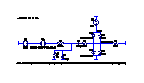
\includegraphics[width=\textwidth]{images/ltspice/jac/shortcircuit-recv.eps}
    \caption[\code{LTspice}-Schema f\"ur Klemmenschaltung]{
        Simulationsschema f\"ur die Simulation  der Klemme am Empf\"anger.\protect\\
        Dateipfad: \code{ltspice/short/receiver.asc}%
    }
    \label{fig:ltspice:shortCircuit:receiver}
\end{figure}

Abbildung \ref{fig:ltspice:shortCircuit:receiver} zeigt die \code{LTspice}-Schaltung,
welche zur Simulation benutzt wird.
Das ankommende  Signal  wird  durch   einen  negativen  Spannungspuls  von
\SI{-45}{\volt}   am   Eingang   simuliert   (Leerlaufspannung   eines
PV-Moduls),  welche  die  ankommende DC-Spannung  von  \SI{900}{\volt}
einbrechen   l\"asst. In der Leitung ist eine parasit\"are Induktivit\"at
von \SI{100}{\micro\henry} eingebaut

Ebenfalls gezeigt  ist eine  Ohm'sch-kapazitive Last von  \SI{1}{\kilo\ohm} ||
\SI{100}{\micro\farad}. Die  Simulationsergebnisse ohne  Last  sind im  oberen
Plot in  Abbildung \ref{fig:simu:short:recv} gezeigt;  der untere Plot  in der
gleichen Abbildung  zeigt das  simulierte Verhalten der  Schaltung mit  der in
Abbildung \ref{fig:ltspice:shortCircuit:receiver} gezeigten Last.

Auf  der  rechten  Seite  ist   ein  Pull-down  Widerstand  auf  \code{Ground}
eingebaut,  um einen  definierten  Signalpegel zu  haben. Dies  ist f\"ur  die
Simulation notwendig, geh\"ort aber nicht per se zur Klemmenschaltung.

\clearpage
\begin{figure}[h!tb]
    \centering
    \begin{tikzpicture}
    \begin{scope}[x={(0mm,0.95\textwidth)},y={(0mm,100mm)}]
        \begin{axis}[%
            title=Klemmenschaltung Spannung am Empf\"anger{,} ohne Last,
            height=45mm,
            width=0.95\textwidth,
            at={(0,50mm)},
            grid=both,
            xlabel=Zeit (\si{\milli\second}),
            ylabel=Spannung (\si{\volt}),
            change x base=true,
            x SI prefix=milli,
            xmin = 0,
            xmax = 3e-4,
            %yticklabel={\num[round-mode=places, round-precision=4]{\tick}},
        ]
        \addplot[-,blue] table[x=time, y=V(receiver)] {data/short-circuit/shortcircuit-recv--noload.dat};
            %\addplot[-,magenta] table[x=time, y=powerModule] {data/short-circuit/shortcircuit-transmitter-PPeak.dat};
            %\legend{MOSFET,PV-Modul};
        \end{axis}
        \begin{axis}[%
            title=Klemmenschaltung Spannung am Empf\"anger{,} Last: \SI{1}{\kilo\ohm}{,} \SI{100}{\micro\farad},
            height=45mm,
            width=0.95\textwidth,
            at={(0,0)},
            grid=both,
            xlabel=Zeit (\si{\second}),
            ylabel=Spannung (\si{\volt}),
            xmin = 0,
            xmax = 5,
            %change x base=true,
            %x SI prefix=micro,
            %yticklabel={\num[round-mode=places, round-precision=4]{\tick}},
        ]
        \addplot[-,blue] table[x=time, y=V(receiver)] {data/short-circuit/shortcircuit-recv--1kohm100uF--10s.dat};
            %\addplot[-,magenta] table[x=time, y=powerModule] {data/short-circuit/shortcircuit-transmitter-PPeak.dat};
            %\legend{MOSFET,PV-Modul};
        \end{axis}
   \end{scope}
\end{tikzpicture}

    \caption[Simulationsergebnisse Klemmenschaltung]{%
        Simulation   Empf\"anger. Die   obere   Kurve  ist   das   Signal   am
        Empf\"anger  ohne  angeschlossene Last. Der  \"Ubertragungsvorgang  im
        unteren  Bild beginnt  bei einer  Sekunde. Die Schaltungsfrequenz  ist
        \SI{10}{\kilo\hertz}%
    }
    \label{fig:simu:short:recv}
\end{figure}

Wie  an  Abbildung  \ref{fig:simu:short:recv}  gesehen werden  kann,  hat  die
Art  der  angeh\"angten Last  einen  merklichen  Einfluss auf  das  ankommende
Signal. Ein grosser kapazitiver Anteil in der Last reduziert die Amplitude des
ankommenden  Signals  bedeutend und  f\"uhrt  einen  sehr lange  (etwa  f\"unf
Sekunden!) dauernden Entlade- und Ladevorgang der kapazitiven Anteile im Kreis
ein.


% ---------------------------------------------------------------------------- %
\clearpage
\subsection{Gesamtsystem}
\label{subsec:simu:ask:total}
% ---------------------------------------------------------------------------- %


Im  Folgenden   werden  der  oben  untersuchte   Transmitter  und  Empf\"anger
in  den  bereits  in  Abschnitt  \ref{sec:simu:model:module:string}  ab  Seite
\pageref{sec:simu:model:module:string}   vorgestellten   Modulstrang  aus   20
Modulen  mit  einer  \SI{20}{\meter} langen  Anschlussleitung  (pro  Richtung)
eingebaut und das Verhalten dieses Systems untersucht.

Die zugeh\"orige  Simulationsschaltung f\"ur  \code{LTspice} ist  in Abbildung
\ref{fig:ltspice:shortcircuit:complete} dargestellt.

\begin{figure}[h!tb]
    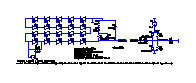
\includegraphics[width=\textwidth]{images/ltspice/jac/shortcircuit.eps}
    \caption[\code{LTspice}-Schaltung f\"ur Kurzschlussmethode, Modulstrang]
    {%
        Gesamte Simulationsschaltung f\"ur die Kurzschlussmethode\protect\\
        Dateipfad: \code{ltspice/short/string.asc}%
    }
    \label{fig:ltspice:shortcircuit:complete}
\end{figure}

\begin{figure}[h!tb]
    \centering
    \begin{tikzpicture}
    \begin{scope}[x={(0mm,0.95\textwidth)},y={(0mm,110mm)}]
        \begin{axis}[%
            title=Klemmenschaltung Spannung am Empf\"anger{,} \code{Rload} {=} \SI{1}{\kilo\ohm},
            height=50mm,
            width=0.95\textwidth,
            at={(0,55mm)},
            grid=both,
            xlabel=Zeit (\si{\micro\second}),
            ylabel=Spannung (\si{\volt}),
            change x base=true,
            x SI prefix=micro,
            legend cell align = left,
            xmin = 0,
            xmax = 3e-4,
            %yticklabel={\num[round-mode=places, round-precision=4]{\tick}},
        ]
        %\addplot[-,blue] table[x=time, y=V(receiver)] {data/short-circuit/shortcircuit-Cload-steps.dat};
        \addplot[-,blue] table[x=time, y=V(receiver)] {data/short-circuit/shortcircuit-Cload-1n.dat};
        %\addplot[-,magenta] table[x=time, y=V(receiver)] {data/short-circuit/shortcircuit-Cload-10n.dat};
        \addplot[-,cyan] table[x=time, y=V(receiver)] {data/short-circuit/shortcircuit-Cload-100n.dat};
        %\addplot[-,purple] table[x=time, y=V(receiver)] {data/short-circuit/shortcircuit-Cload-1u.dat};
        \addplot[-,solarized-magenta] table[x=time, y=V(receiver)] {data/short-circuit/shortcircuit-Cload-10u.dat};
        \legend{%
            $\mathrm{C_{load}} = \SI{1}{\nano\farad}$,
            $\mathrm{C_{load}} = \SI{100}{\nano\farad}$,
            $\mathrm{C_{load}} = \SI{1000}{\nano\farad}$%
        };
            %\addplot[-,magenta] table[x=time, y=powerModule] {data/short-circuit/shortcircuit-transmitter-PPeak.dat};
            %\legend{MOSFET,PV-Modul};
        \end{axis}
        \begin{axis}[%
            title=Klemmenschaltung Spannung am Empf\"anger{,} \code{Cload} {=} \SI{100}{\nano\farad},
            height=50mm,
            width=0.95\textwidth,
            at={(0,0)},
            grid=both,
            xlabel=Zeit (\si{\micro\second}),
            ylabel=Spannung (\si{\volt}),
            change x base=true,
            x SI prefix=micro,
            legend cell align = left,
            xmin = 0,
            xmax = 3e-4,
            %yticklabel={\num[round-mode=places, round-precision=4]{\tick}},
        ]
        %\addplot[-,blue] table[x=time, y=V(receiver)] {data/short-circuit/shortcircuit-Rload-10.dat};
        \addplot[-,blue] table[x=time, y=V(receiver)] {data/short-circuit/shortcircuit-Rload-100.dat};
        \addplot[-,cyan] table[x=time, y=V(receiver)] {data/short-circuit/shortcircuit-Rload-1k.dat};
        \addplot[-,solarized-magenta] table[x=time, y=V(receiver)] {data/short-circuit/shortcircuit-Rload-10k.dat};
        \legend{%
            %$\mathrm{R_{load}} = \SI{10}{\ohm}$,
            $\mathrm{R_{load}} = \SI{100}{\ohm}$,
            $\mathrm{R_{load}} = \SI{1}{\kilo\ohm}$,
            $\mathrm{R_{load}} = \SI{10}{\kilo\ohm}$%
        };
            %\addplot[-,magenta] table[x=time, y=powerModule] {data/short-circuit/shortcircuit-transmitter-PPeak.dat};
            %\legend{MOSFET,PV-Modul};
        \end{axis}
   \end{scope}
\end{tikzpicture}

    \caption[Simulationsergebnisse Kurzschlussmethode]{%
        Simulationsergebnisse  f\"ur  das  Signal  am  Knoten  \code{RECEIVER}
        aus  Abbildung  \ref{fig:ltspice:shortcircuit:complete}  f\"ur  Lasten
        mit   verschiedenen    kapazitiven   Anteilen    \code{Cload}   (obere
        Plots)  und  resistiven   Anteilen  \code{Rload}  (untere  Plots). Die
        \"Ubertragungsfrequenz betr\"agt \SI{10}{\kilo\hertz}.%
    }
    \label{fig:simu:short:complete}
\end{figure}

Wie   in   Abbildung   \ref{fig:simu:short:complete}   zu   sehen,   hat   die
angeschlossene   Last  einen   betr\"achtlichen  Einfluss   auf  das   Signal,
welches  beim  Empf\"anger  ankommt  (wie  auch  schon  im  vorigen  Abschnitt
beobachtet).   Bei einem  Ohm'schen Lastwiderstand  von \SI{1}{\kilo\ohm}  und
einer Lastkapazit\"at  von bereits  \SI{100}{\nano\farad} kommt  anstatt eines
Rechteckpulses eine Doppelschwingung beim  Empf\"anger an; steigt die Gr\"osse
der parasit\"aren Komponente der Last auf \SI{1}{\milli\farad}, ist vom Signal
am Empf\"anger bei der eingestellten Frequenz nicht mehr viel zu sehen.

Auch die  Ohm'sche Komponente der  Last hat  bedeutenden Einfluss; ist  sie zu
klein, sinkt die Signalamplitude am  Empf\"anger stark (blaue Kurve im unteren
Plot von Abbildung \ref{fig:simu:short:complete}).

Die Gesamtbeurteilung  dieses Ansatzes  ist gemischt: Prinzipiell  k\"onnte es
m\"oglich sein, eine  funktionierende Implementation zu entwickeln. Allerdings
gibt  es  Faktoren,  welche  erhebliche Auswirkungen  auf  die  Erfolgschancen
aus\"uben haben,  und die wir  nicht beeinflussen k\"onnen, oder  deren genaue
Untersuchung im Rahmen  dieses Projekts aus Zeit-  und Materialgr\"unden nicht
m\"oglich ist.

Sollte   diese   L\"osungsvariante   implementiert  werden,   m\"ussten
detailliertere Untersuchungen  gemacht werden. Nicht nur muss  das Verhalten des
PV-Moduls (bzw. des Modulstrangs) bekannt  sein, es m\"ussen auch detaillierte
Informationen \"uber die angeh\"angten  Lasten eingeholt werden.  Insbesondere
muss das  Verhalten des  Wechselrichters unter  verschiedenen Betriebsbedingen
(Last,   momentane   Leistung   der  PV-Modulstr\"ange,   allenfalls   weitere
unbekannte  Parameter)  bekannt   sein. Abh\"angig  von  den  Charakteristiken
der  gesamten mit  dem  Modulstrang verbundenen  Schaltung  k\"onnte es  sein,
dass  diese L\"osungsvariante  nicht  implementierbar  ist. Oder es  m\"ussten
m\"oglicherweise weitere Schaltkreise entwickelt  und eingebaut werden, um mit
dem Verhalten des Wechselrichters und  den an ihn angeh\"angten Lasten korrekt
umgehen  zu k\"onnen. Dies  wiederum  w\"are nicht  wirklich  im Sinne  dieser
L\"osung, da ihre grosse Attraktivit\"at  genau darin liegen w\"urde, dass ihr
Schaltungs- und Materialaufwand (theoretisch) sehr gering ist.

Grunds\"atzlich finden wir diese  L\"osungsvariante aufgrund des enorm simplen
Prinzips zwar sehr interessant. Da dies  jedoch (soweit uns bekannt) absolutes
Neuland ist und wir die Ressourcen  nicht haben, um einen Modulstrang oder das
an  einen Modulstrang  angeh\"angte System  genau genug  zu untersuchen  (also
ausmessen statt  lediglich simulieren),  beurteilen wir  unsere Erfolgschancen
mit dieser Methode als gering.


% ---------------------------------------------------------------------------- %
\clearpage
\section{Schlussfolgerungen}
\label{subsec:simu:conclusion}
% ---------------------------------------------------------------------------- %

Die  in  den  vorigen  Abschnitten gemachten  Beobachtungen  sind  in  Tabelle
\ref{tab:simu:conclusion} in einer \"Ubersicht zusammengefasst.

Die Kurzschlussvariante  wird aufgrund der starken  Lastabh\"angigkeit und der
Neuartigkeit des  Konzepts nicht weiterverfolgt. Wie bereits  angemerkt halten
wird  diesen  Ansatz  zwar  f\"ur sehr  interessant,  beurteilen  aber  unsere
Erfolgschancen  im  Rahmen eines  Semesterprojekts  als  zu gering,  um  diese
Variante weiter zu verfolgen.

Bei der  kapazitiven Einkopplung hat  der Ort, an  dem die Einkopplung  in den
Strang erfolgt, einen grossen Einfluss  nicht nur auf die Signalamplitude beim
Empf\"anger, sondern auch  auf die Form des Signals. Dies  beurteilen wird als
nicht  optimal, da  allenfalls  komplexe L\"osungen  n\"otig  w\"aren, um  das
Signal am Empf\"anger \"uberhaupt noch als solches erkennen zu k\"onnen.

Aufgrund der niedrigen  Verzerrung des Signals bei  der induktiven Einkopplung
wird diese  Variante implementiert. Die Signalamplitude beim  Betrieb in einem
Strang mit mehreren Modulen kann zwar  stark abfallen, jedoch ist selbst unter
diesen  Umst\"anden  das Signal  prinzipiell  noch  sehr sauber  und  k\"onnte
allenfalls wieder herausgefiltert  und verst\"arkt werden. Alternativ k\"onnte
in einer weiteren Entwicklungsstufe eine L\"osung implementiert werden, welche
den Strang, in  dem ein Sensor installiert ist, ausmisst,  und automatisch bei
der optimalen Frequenz (innerhalb von spezifizierten Grenzen) sendet.

\vspace*{2em}

\begin{table}[h!tb]
    \centering
    \small
    \caption{Gegen\"uberstellung der drei L\"osungsvarianten}
    \label{tab:simu:conclusion}
    \begin{tabular}{p{38mm}p{28mm}p{28mm}p{28mm}}
        \toprule
        \textsc{Kriterium} &
        \parbox[t]{27mm}{\textsc{induktive\\Kopplung}} &
        \parbox[t]{27mm}{\textsc{kapazitive\\Kopplung}} &
        \textsc{Kurzschluss} \\

        \midrule

        Komplexit\"at der Schaltung &
        mittel &
        mittel &
        simpel \\
        [7mm]

        \rowcolor{solarized-base2}
        Neuartigkeit des Konzepts &
        niedrig &
        niedrig &
        hoch \\
        [7mm]

        Kosten &
        hoch &
        mittel &
        klein  \\
        [7mm]

        \rowcolor{solarized-base2}
        St\"arke des Signals am Empf\"anger &
        bei Resonanz gut, kann sonst stark abfallen &
        variiert stark mit Position im Strang &
        variiert stark mit Last \\
        [7mm]

        Verzerrung des Signals am Empf\"anger &
        schwache Verzerrung &
        variiert mit Position im Strang, Signal kann sehr stark verzerrt werden &
        variiert stark mit Last \\
        \bottomrule
    \end{tabular}
\end{table}

% **************************************************************************** %
\chapter{Hardware}
\label{chap:hardware}
% **************************************************************************** %


Dieses  Kapitel dokumentiert  die  Komponentenwahl  und das  Schaltungs-Design
der  Sensorplatine  und  des  Master-Ger\"ats.   Die  wichtigsten  Komponenten
werden vorgestellt,  ihre Auswahl begr\"undet und  die n\"otigen Beschaltungen
erkl\"art. Es wird ebenfalls auf kritische Punkte bei der Hardware-Entwicklung
eingegangen.

{\begin{a3pages}
% ---------------------------------------------------------------------------- %
\section{Sensorplatine}
\label{sec:hw:sensorplatine}
% ---------------------------------------------------------------------------- %
    \setlength{\parindentbak}{\parindent}

    \noindent\adjustbox{valign=t}{\begin{minipage}{135mm}
        Das  Sensorboard  besteht  aus  einer   CPU, welche  alle  Komponenten
        koordiniert, einem  Modulator und einem Demodulator  zur Kommunikation
        und  einem  Buck-Konverter,  der  die  Netzspannung  f\"ur  das  Board
        transformiert.

        \setlength{\parindent}{\parindentbak}
        Als   CPU  dient   ein  Atmel   SAM  D09   (Bereich  3   in  Abbildung
        \ref{fig:sensor:schema:highlights}). Dieser  wird  verwendet, weil  er
        der g\"unstigste Prozessor  in seiner Klasse ist  und alle notwendigen
        Funktionen  mitbringt. Der   Mikrochip  hat  einen  12   Bit-ADC,  ein
        CRC-Modul,  eine  32  Bit  ARM-Architektur und  braucht  extrem  wenig
        Leistung.

        Zum  Speisen  des  Boards  wird ein  LMR16006  von  Texas  Instruments
        verwendet (Bereich 1 in Abbildung \ref{fig:sensor:schema:highlights}).
        Dieser kann  die gesamte  Spanne der Modulspannung  von \SI{12}{\volt}
        bis \SI{60}{\volt}  ohne Probleme auf  \SI{3.3}{\volt} transformieren,
        welche das Board versorgt.

        Als Modulator  dient ein Voltage  Controlled Oscillator (VCO)  auf dem
        74HC4640-Chip von Texas Instruments (Bereich  2).  Dieser kann mit der
        richtigen Beschaltung  Frequenzen von  wenigen Kilohertz  bis mehreren
        Megahertz erzeugen.

        Zum Demodulieren wird ein einfaches Tiefpassfilter mit einer Diode und
        einem Verst\"arker benutzt (Bereich 6).

        Die  Messung der  Versorgungsspannung  ist  mit einem  Spannungsteiler
        implementiert,    zu   finden    in    Bereich    4   von    Abbildung
        \ref{fig:sensor:schema:highlights}.

        Bereich  5  enth\"alt   zwei  LEDs  und  einen   Schalter,  welche  zu
        Statusangaben und Debuggen am Sensor direkt verwendet werden k\"onnen.

        Im Folgenden werden die einzelnen Teilschaltungen dokumentiert und die
        Komponentenwahl begr\"undet.

        \adjustbox{valign=t}{\begin{minipage}{0.475\textwidth}
            \centering
            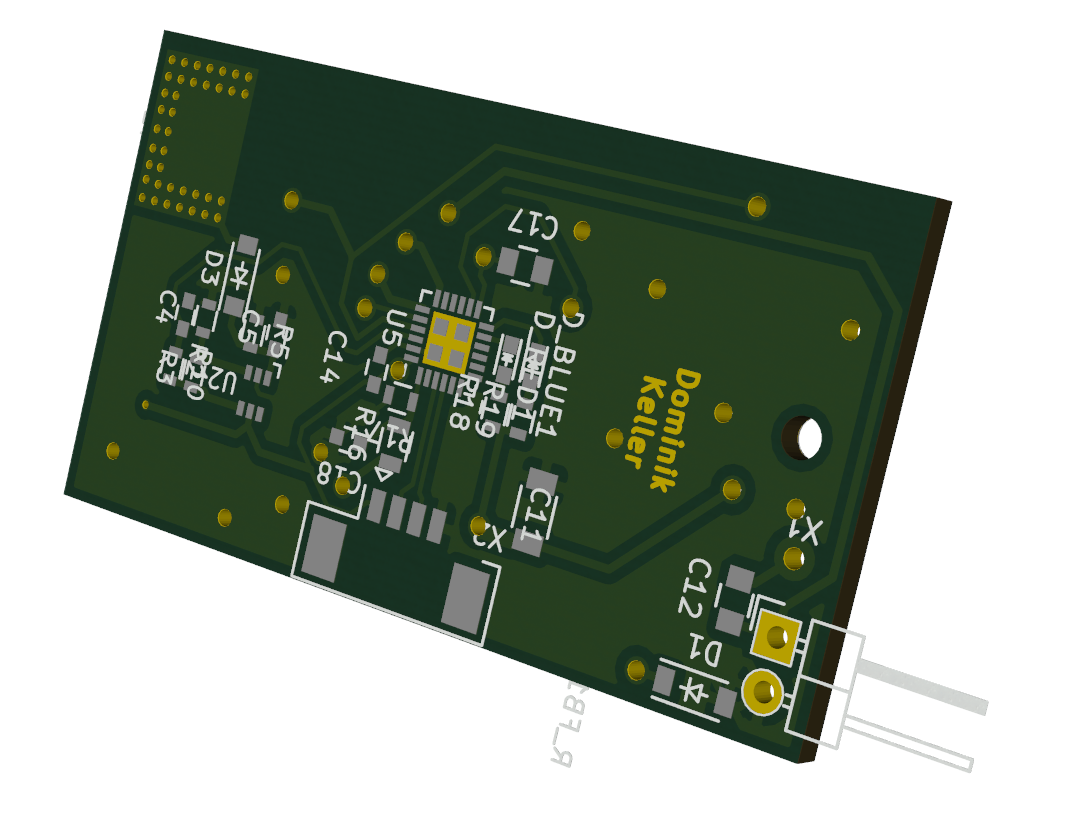
\includegraphics[width=0.9\textwidth]{images/sensor-pcb/sensor-3d-front.png}
            \figcaption[Sensor: Vorderseite PCB]{PCB, Vorderseite}
            \label{fig:sensor:pcb:front}
        \end{minipage}}
        \adjustbox{valign=t}{\begin{minipage}{0.475\textwidth}
            \centering
            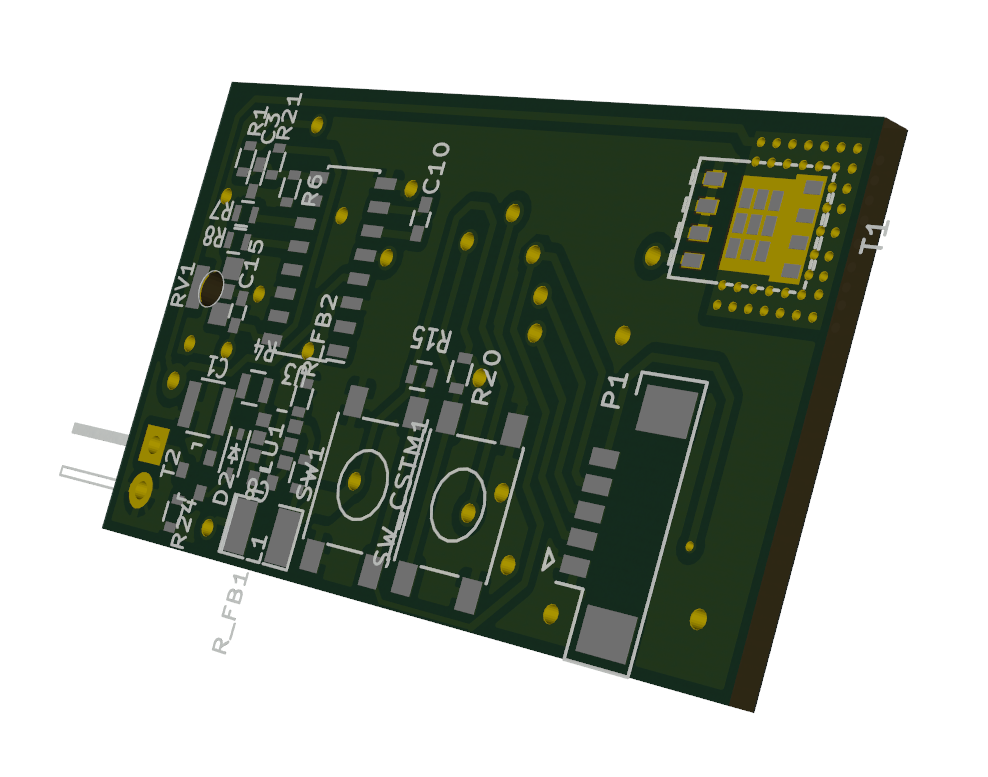
\includegraphics[width=0.9\textwidth]{images/sensor-pcb/sensor-3d-back.png}
            \figcaption[Sensor: R\"uckseite PCB]{PCB, R\"uckseite}
            \label{fig:sensor:pcb:back}
        \end{minipage}}
    \end{minipage}}
    \hspace*{15mm}
    \adjustbox{valign=t}{\begin{minipage}{195mm}
        \centering
        \includegraphics[width=\textwidth]{images/sensor-sch/sensor--sch--highlights.eps}%
        \figcaption[Schema Sensor, \"Ubersicht]{%
            Schema   des   \Sensor   s. Eine  Grossversion   ist   in   Anhang
            \label{app:chap:schemas}  zu  finden,   die  einzelnen  Baugruppen
            sind  in  den  folgenden  Abschnitten  beschrieben  und  gr\"osser
            abgebildet.%
        }
        \label{fig:sensor:schema:highlights}
    \end{minipage}}
\end{a3pages}}


% ---------------------------------------------------------------------------- %
\subsection{Speisung}
\label{subsec:hw:sensor:supply}
% ---------------------------------------------------------------------------- %

Die  Speisung  der  Schaltung   \"ubernimmt  ein  LMR16006. Er  verkraftet  am
Input   bis   \SI{63}{\volt}   und   sollte   so   die  an   handels\"ublichen
PV-Modulen    anliegenden   Spannungen    verkraften   (siehe    auch   Anhang
\ref{app:commercial:modules} auf  Seite \pageref{app:commercial:modules}).  Er
kommt auch  mit 4  Volt am  Eingang noch  klar. Da die  Versorgungsspannung im
Verlauf des  Tages zwischen \SI{12}{\volt} und  \SI{60}{\volt} schwanken kann,
ist der LMR16006 soweit bestens f\"ur unsere Schaltung geeignet.

Er  hat einen  sehr konstanten  Wirkungsgrad von  70 bis  80 Prozent,  je nach
Speisespannung.

Der  LMR16006 kann  maximal  \SI{600}{\milli\ampere}  liefern, was  ausreicht,
wenn  man   einen  genug  grossen  Pufferkondensator   f\"ur  Leistungsspitzen
einbaut   (\SI{10}{\micro\farad}  in   unserem  Fall,   rechts  in   Abbildung
\ref{fig:hw:sensor:speisung}).

Zudem  hat  dieser  Spannungsregler  einen  typischen  Quiescent  Current  von
nur  \SI{28}{\micro\ampere}. Damit  ist  er  auch  extrem  stromsparend.   Die
Beschaltung  wurde  nach   Empehlung  des  Datenblatts  \cite{ref:ti:lmr16006}
gew\"ahlt,  welche   garantiert,  dass  Powerspikes  gut   abgefangen  werden.
$R_{\mathrm{FB1}}$  und  $R_{\mathrm{FB2}}$  wurden  im  Verh\"altnis  $1:3.3$
gew\"ahlt, da \SI{3.3}{\volt} die Spannung ist, die wir am Ausgang anstreben.

Der Active  Low Shutdown Pin wird  dauernd auf High gezogen,  damit der Regler
immer an ist sobald am Eingang Spannung anliegt.

Damit die  Montage einfacher  ist, ist ein  Verpolungsschutz eingebaut. Dieser
besteht aus einem P-Fet, einer  Zenerdiode und einem Gate-Vorwiderstand (linke
Seite in Abbildung \ref{fig:hw:sensor:speisung}).

\vspace*{2em}

\begin{figure}[h!t]
    \centering
    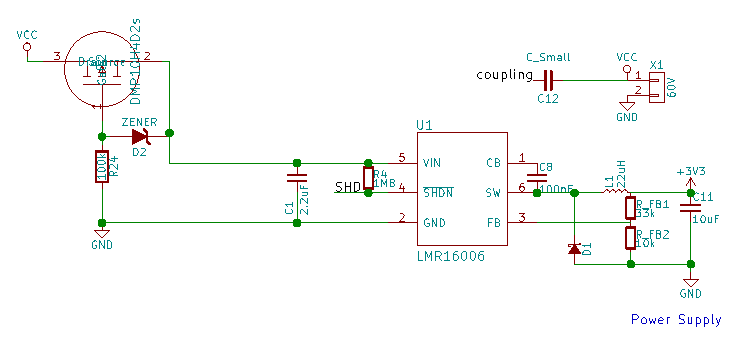
\includegraphics[width=1\textwidth]{images/sensor-sch/sensor--sch--supply.eps}
    \caption[Sensor: Schema Speisung]{Speisung Sensor}
    \label{fig:hw:sensor:speisung}
\end{figure}


% ---------------------------------------------------------------------------- %
\clearpage
\subsection{Transmitter}
\label{subsec:hw:sensor:transmitter}
% ---------------------------------------------------------------------------- %

Der  Transmitter  besteht  aus  einem   einfachen  VCO,  der  das  Signal  auf
die  Spannungsversorgung aufmoduliert.   Daf\"ur  wird am  $VCO_{\mathrm{in}}$
mithilfe eines Spannungsteilers eine fixe Spannung angelegt. Mit der korrekten
Wahl von \code{R7},  \code{R8} und \code{C10} kann  die Resonanzfrequenz f\"ur
die Leitung erreicht werden, mit der  dann moduliert wird. Diese Werte sind so
gew\"ahlt,  wie es  die  Graphen im  Datenblatt \cite{ref:ti:cd54}  zeigen. Es
wird  eine Frequenz  von  \SI{20}{\mega\hertz}  ausgew\"ahlt. Das Signal  wird
moduliert, indem der UART \code{TX} Pin  direkt am \code{INH} Pin den VCO ein-
und  ausschaltet  und  somit  ein  On-Off  Keying zustande  bringt. Hier  ist
wichtig, dass der Pin Active High ist.

\begin{figure}[h!t]
    \centering
    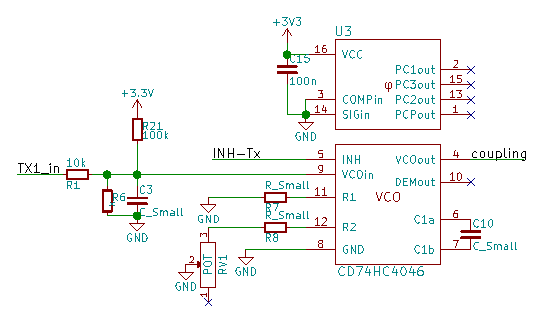
\includegraphics[width=0.70\textwidth]{images/sensor-sch/sensor--sch--transmitter.eps}
    \caption[Sensor: Schema Transmitter]{Transmitter Sensor}
\end{figure}


% ---------------------------------------------------------------------------- %
\subsection{Microcontroller}
\label{subsec:hw:sensor:mcu}
% ---------------------------------------------------------------------------- %

\begin{wrapfigure}{r}{0.6\textwidth}
    \centering
    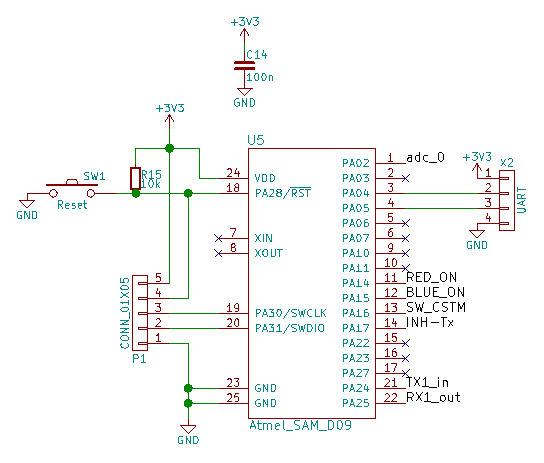
\includegraphics[width=0.60\textwidth]{images/sensor-sch/sensor--sch--mcu.eps}
    \caption[Sensor: Schema Microcontroller]{Microcontroller Sensor}
\end{wrapfigure}

Der  Mikrokontroller  braucht  bis  auf  einen  Pull-Up-Widerstand  am  Active
Low  Reset und  einem  Stabilisierungskondensator  an der  Spannungsversorgung
keine  spezielle  Beschaltung. Der  Mikrochip  ist  so  beschaltet,  dass  die
beiden  UART-Linien  verf\"ugbar sind;  eine  zum  Senden \"uber  die  Leitung
und  eine  zum   Debuggen. Ebenfalls  zu  einem  Stecker   verbunden  ist  die
Programmierschnittstelle (SWD). Das Datenblatt  ist unter \cite{ref:atmel:cpu}
verf\"ugbar.



% ---------------------------------------------------------------------------- %
\clearpage
\subsection{Spannungsmessung}
\label{subsec:hw:sensor:voltageSense}
% ---------------------------------------------------------------------------- %

Der  Spannungsteiler  ist  so  eingestellt, dass  am  ADC-Pin  \SI{3.3}{\volt}
anliegen,  wenn  bei  der Spannungsversorgung  \SI{60}{\volt}  anliegen.   Der
Kondensator \code{C18} dient der Gl\"attung des Signals.

\begin{figure}[h!t]
    \centering
    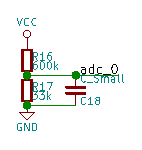
\includegraphics[width=0.25\textwidth]{images/sensor-sch/sensor--sch--sensor.eps}
    \caption[Sensor: Schema Spannungsmessung]{Spannungsmessung Sensor}
\end{figure}


% ---------------------------------------------------------------------------- %
\subsection{Interface}
\label{subsec:hw:sensor:interface}
% ---------------------------------------------------------------------------- %

\begin{figure}[h!t]
    \centering
    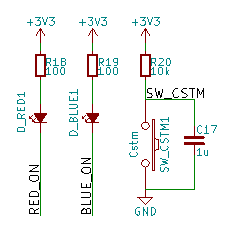
\includegraphics[angle=-90,width=0.4\textwidth]{images/sensor-sch/sensor--sch--interface.eps}
    \caption[Sensor: Schema Interface]{Interface Sensor}
\end{figure}

Am   Sensor  sind   zwei  LEDs   und  ein   Schalter  angebracht,   welche  zu
Statusanzeigen  und zum  Debuggen  benutzt werden  k\"onnen. In der  aktuellen
Firmware-Version  werden  die  LEDs   getoggled,  um  korrektes  Funktionieren
des  Sensors anzuzeigen  (siehe Abschnitt  \ref{subs:Statusanzeige} auf  Seite
\pageref{subs:Statusanzeige}).

% ---------------------------------------------------------------------------- %
\clearpage
\subsection{Empf\"anger}
\label{subsec:hw:sensor:receiver}
% ---------------------------------------------------------------------------- %

Der   Empf\"anger  ist   ein  einfaches   Tiefpassfilter.   Zuerst   wird  das
Eingangssignal,  welches  noch  moduliert   ist,  durch  die  Diode  \code{D3}
gleichgerichtet. Ein dahinter  geschalteter Tiefpass  sorgt daf\"ur,  dass das
Signal gegl\"attet wird. Da  dieses Signal durch Verluste auf  der Leitung und
\"uber der Diode eine viel zu kleine Amplitude hat, wird es zus\"atzlich durch
einen nicht invertierenden Opamp verst\"arkt.

\begin{figure}[h!t]
    \centering
    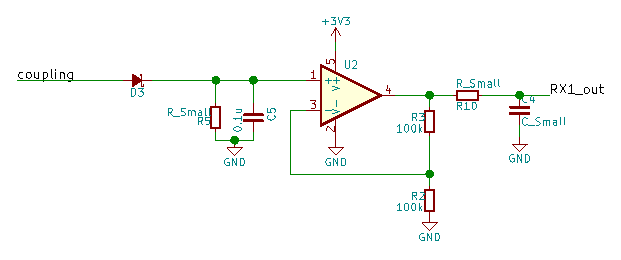
\includegraphics[width=0.9\textwidth]{images/sensor-sch/sensor--sch--receiver.eps}
    \caption[Sensor: Schema Empf\"anger]{Empf\"anger Sensor}
\end{figure}

{\begin{a3pages}
% ---------------------------------------------------------------------------- %
\section{\Master}
\label{sec:hw:master}
% ---------------------------------------------------------------------------- %
    % \parindent is set to 0 inside of minipages. Back up its value and access
    % it inside the minipage.
    \setlength{\parindentbak}{\parindent}

    \noindent\adjustbox{valign=t}{\begin{minipage}{135mm}
        Das \Master~ (Abbildung  \ref{fig:hw:master:photo:master}) basiert auf
        einem  \Raspi~ (Abbildung  \ref{fig:hw:master:photo:raspi}), erweitert
        mit einem zugekauften Touchscreen-Modul  und einem eigens entwickelten
        PCB, welches  f\"ur zus\"atzliche Funktionalit\"at  verantwortlich ist
        (Kommunikation mit Sensoren, Strommessung, GSM-Modem).

        \setlength{\parindent}{\parindentbak} % restore paragraph indentation

        Montiert    ist    das     \Master~in    einem    Hutschienengeh\"ause
        (auch       bekannt       als      DIN-Rail-Geh\"ause,       Abbildung
        \ref{fig:hw:master:photo:dinrail}). Damit   unser   Ger\"at   sinnvoll
        im   Geh\"ause   untergebracht   werden    kann,   ist   eine   eigene
        Frontplatte    entwickelt    und     gefertigt    worden    (Abbildung
        \ref{fig:hw:master:photo:dinrailCover}).

        {\centering
            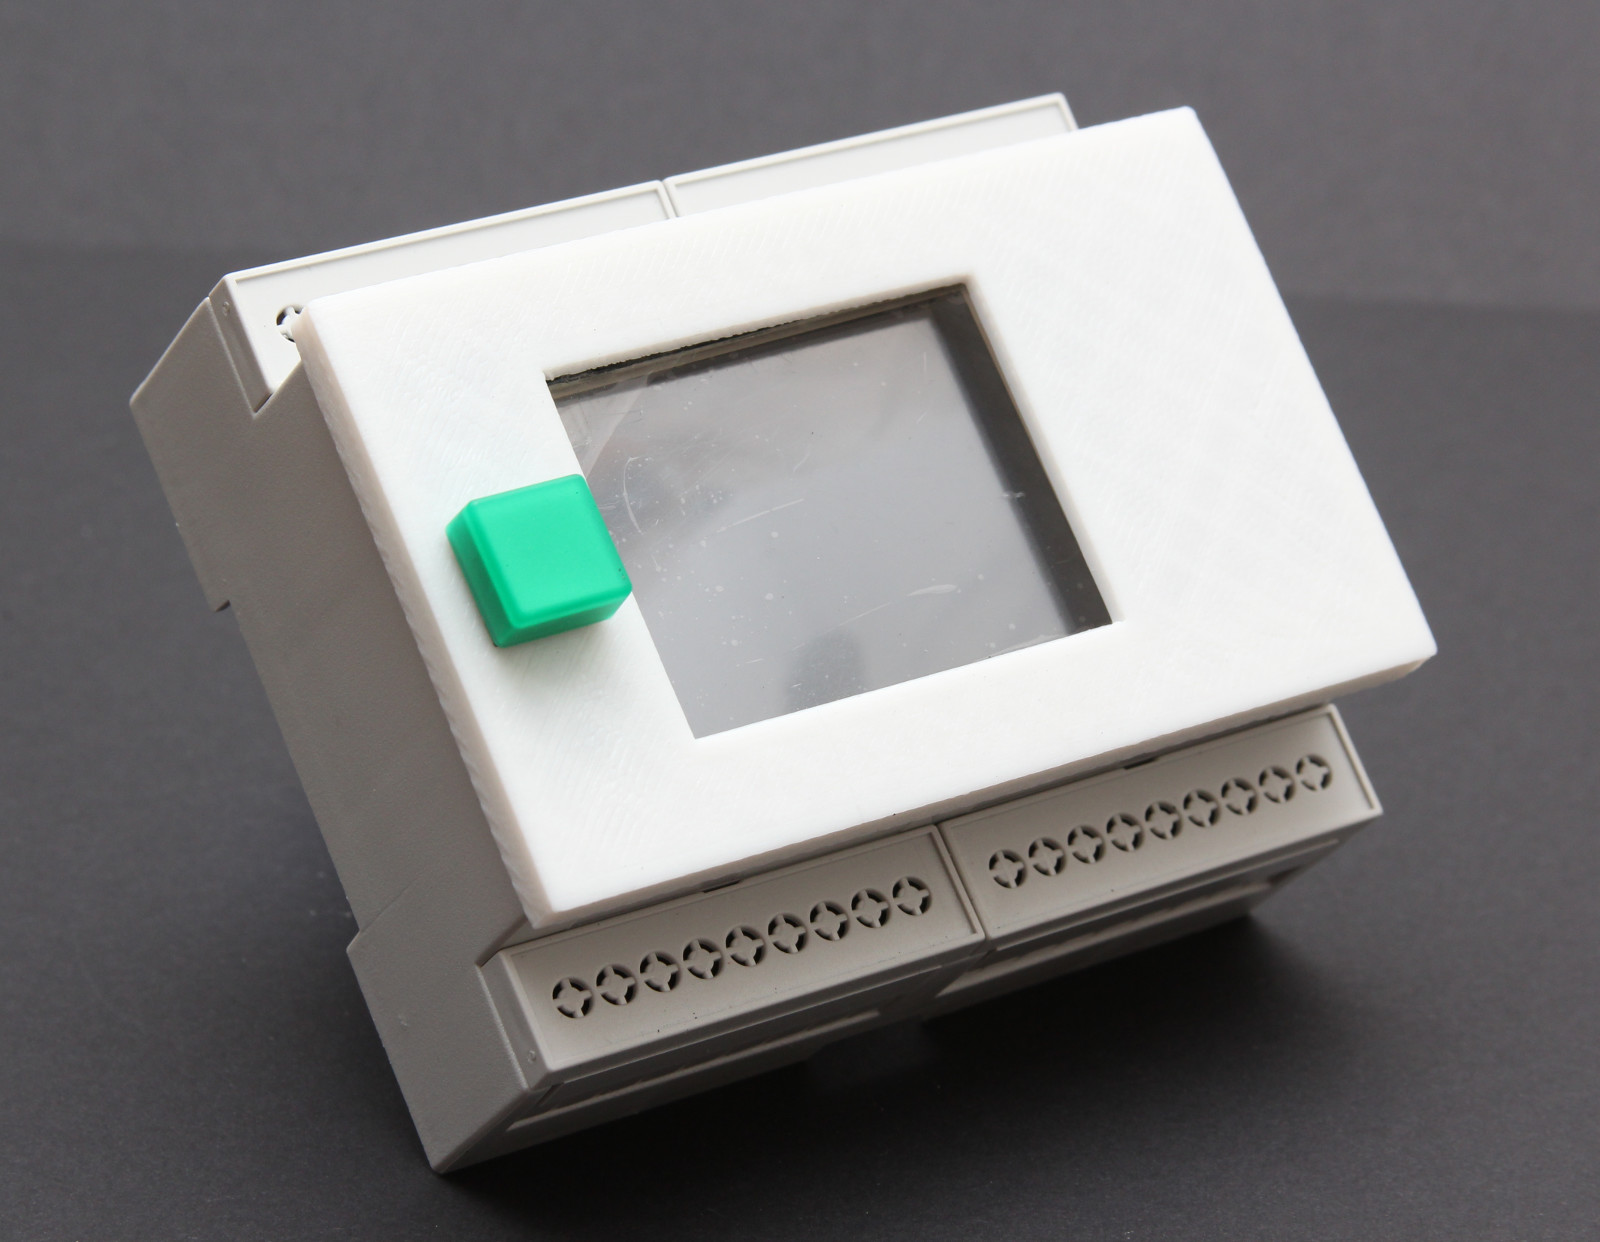
\includegraphics[width=100mm]{images/superv-photos/master.jpeg}
            \figcaption[\Master: Foto zusammengesetzt]{\Master, zusammengesetzt}
            \label{fig:hw:master:photo:master}
            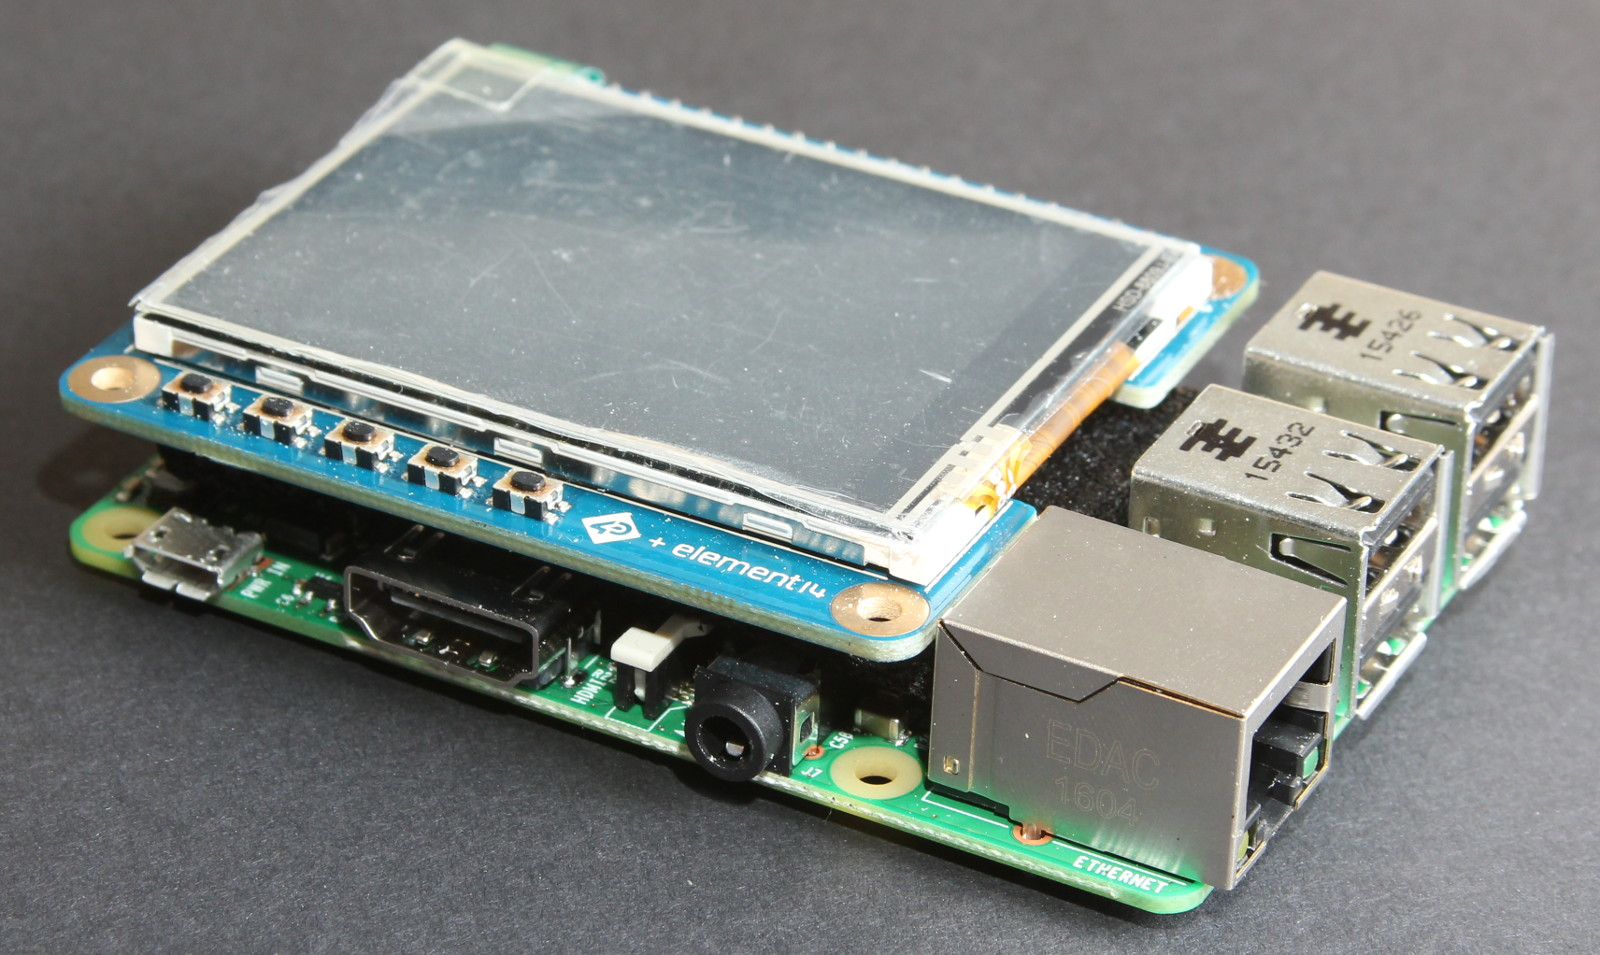
\includegraphics[width=100mm]{images/superv-photos/raspi-1.jpeg}
            \figcaption[\Master: Foto Touchscreen-Modul]{\Raspi~mit aufgestecktem Touchscreen-Modul}
            \label{fig:hw:master:photo:raspi}
        }
    \end{minipage}}
    \hspace*{15mm}
    \adjustbox{valign=t}{\begin{minipage}{195mm}
        \centering
        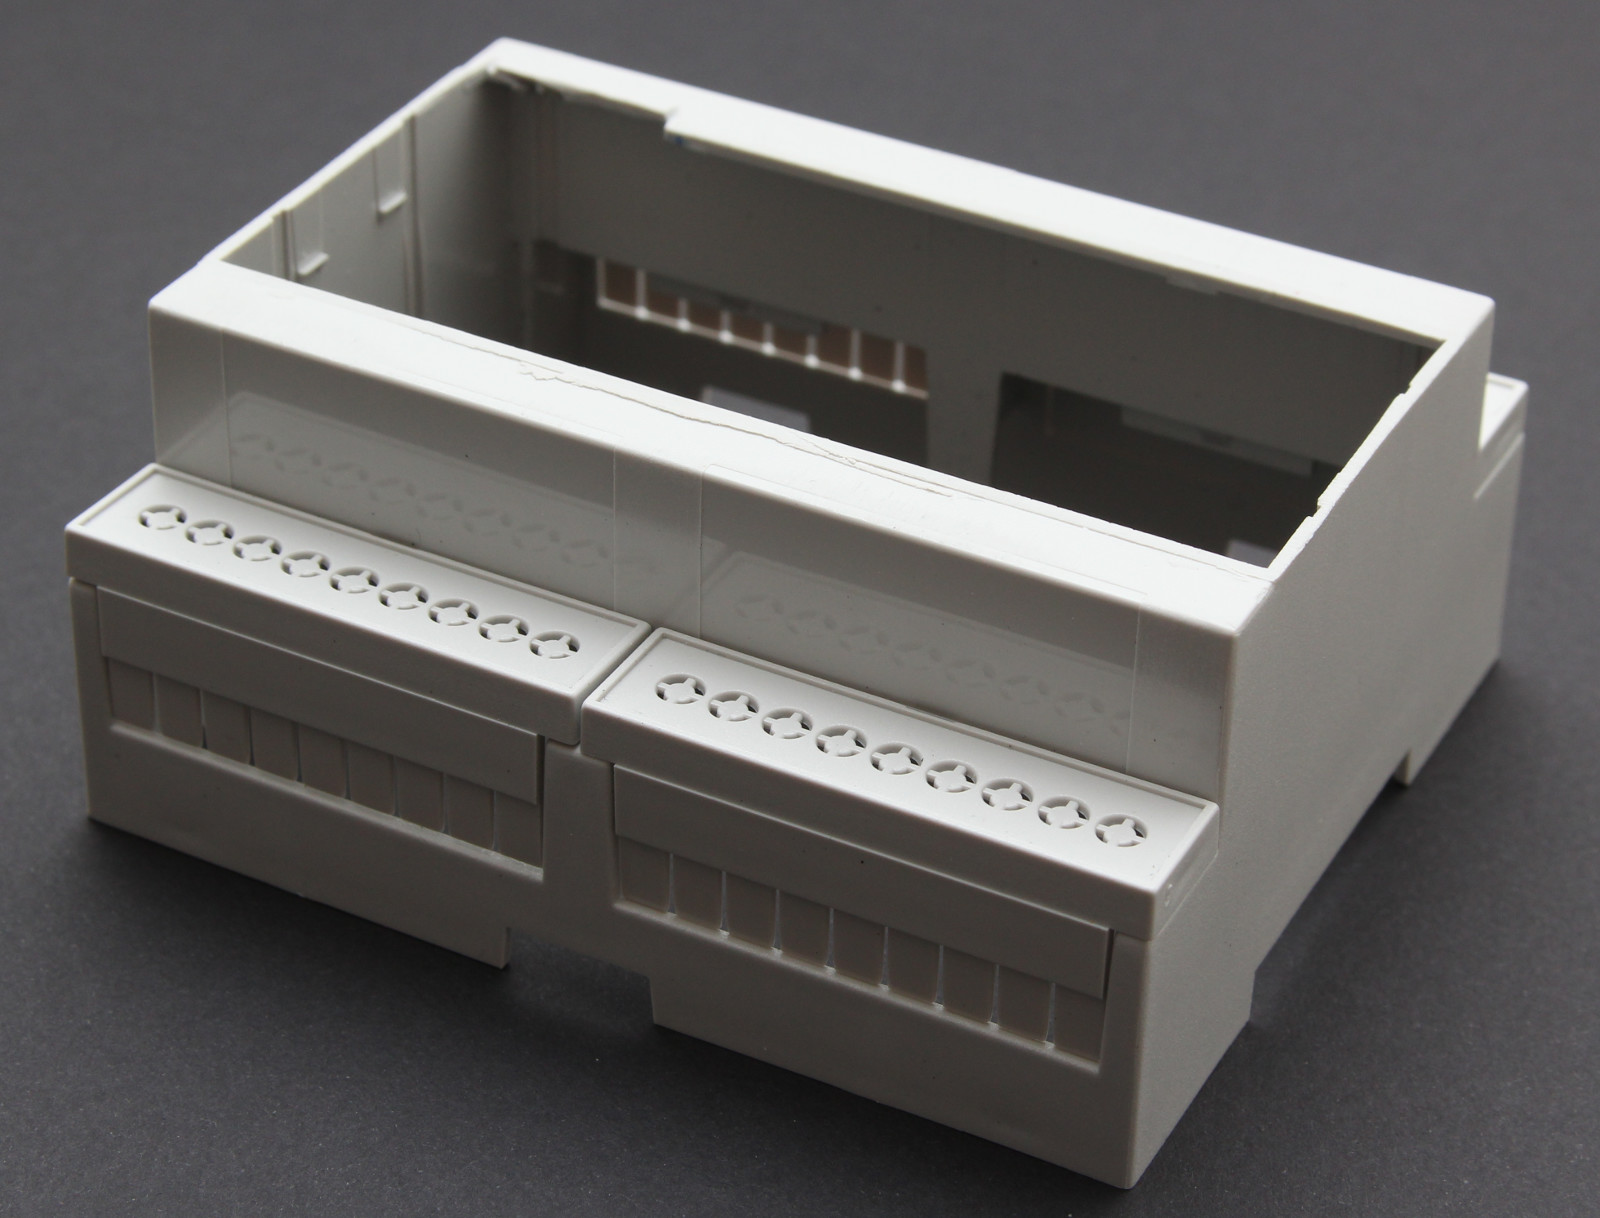
\includegraphics[width=100mm]{images/superv-photos/dinrail.jpeg}
        \figcaption[\Master: Foto Hutschienengeh\"ause]{Hutschienengeh\"ause}
        \label{fig:hw:master:photo:dinrail}
        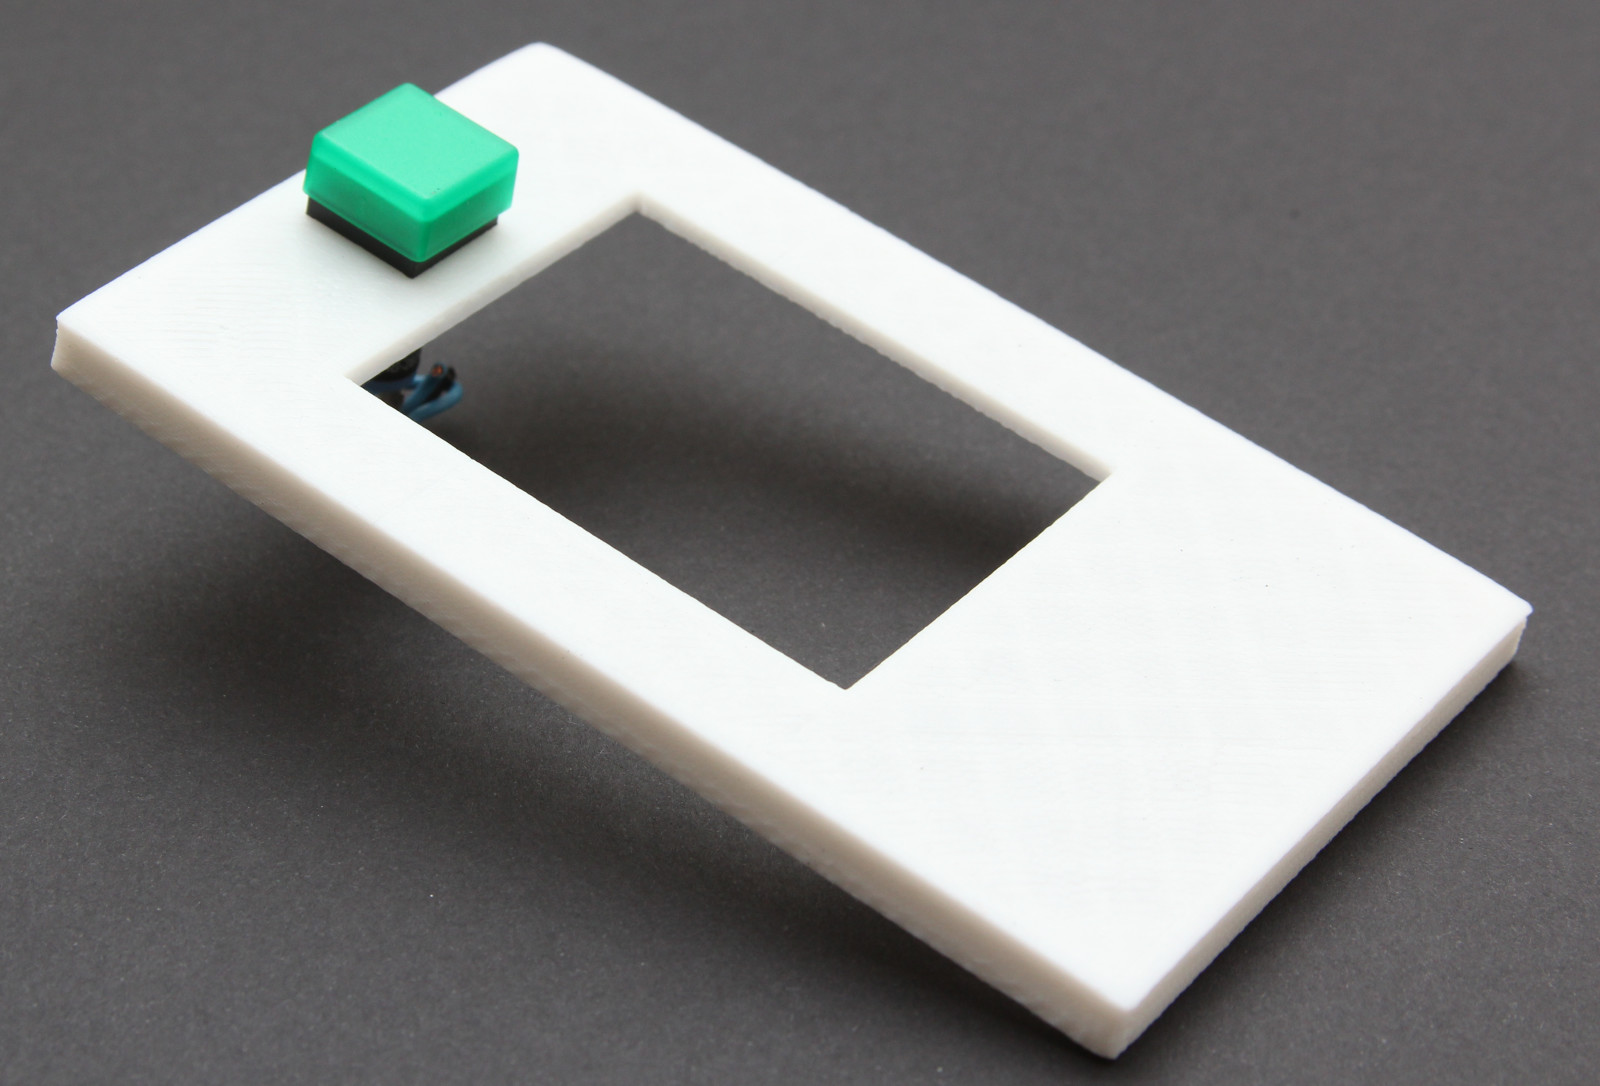
\includegraphics[width=100mm]{images/superv-photos/dinrail-cover.jpeg}
        \figcaption[\Master: Foto Abdeckung]{3D-degruckte Abdeckung f\"ur das Hutschienengeh\"ause}
        \label{fig:hw:master:photo:dinrailCover}
    \end{minipage}}

    \noindent\adjustbox{valign=t}{\begin{minipage}{135mm}
        Abbildung  \ref{fig:master:schema:highlights} zeigt  das Schema  f\"ur
        das   Zusatz-PCB   des  \Master   s. Bereich   1   ist  die   Speisung
        (genauer   dokumentiert  in   Abschnitt  \ref{subsec:hw:master:supply}
        ab  Seite  \pageref{subsec:hw:master:supply}),   allgemeine  Ein-  und
        Ausg\"ange   sind  im   Bereich  2   untergebracht  (siehe   Abschnitt
        \ref{subsec:hw:master:gpio} ab Seite \pageref{subsec:hw:master:gpio}),
        die  Kommunikation  mit den  Sensoren  erfolgt  durch die  Schaltungen
        in   Bereich   3   (Abschnitt   \ref{subsec:hw:master:sensorcomm}   ab
        Seite   \pageref{subsec:hw:master:sensorcomm}),  die   String-Str\"ome
        werden      mit      den      Komponenten      aus      Bereich      4
        gemessen    (Abschnitt    \ref{subsec:hw:master:current}   ab    Seite
        \pageref{subsec:hw:master:current})  und  Bereich   5  beinhaltet  die
        GSM-Schaltung    (Abschnitt   \ref{subsec:hw:master:gsm}    ab   Seite
        \pageref{subsec:hw:master:gsm}).

        \setlength{\parindent}{\parindentbak} % restore paragraph indentation
        Abbildungen  \ref{fig:master:pcb:front} und  \ref{fig:master:pcb:back}
        zeigen  ein  3D-Modell  des  PCB,  auf  welchem  die  Zusatzfunktionen
        untergebracht sind.

        Das  PCB  in  der  aktuellen Konfiguration  kann  drei  Modulstr\"ange
        parallel  verwalten. Das  Hinzuf\"ugen  zus\"atzlicher  Modulstr\"ange
        w\"are  relativ einfach,  w\"urde  aber ein  gr\"osseres  PCB mit  den
        zugeh\"origen zus\"atzlichen Komponenten bedingen.

        \adjustbox{valign=t}{\begin{minipage}{0.475\textwidth}
            \centering
            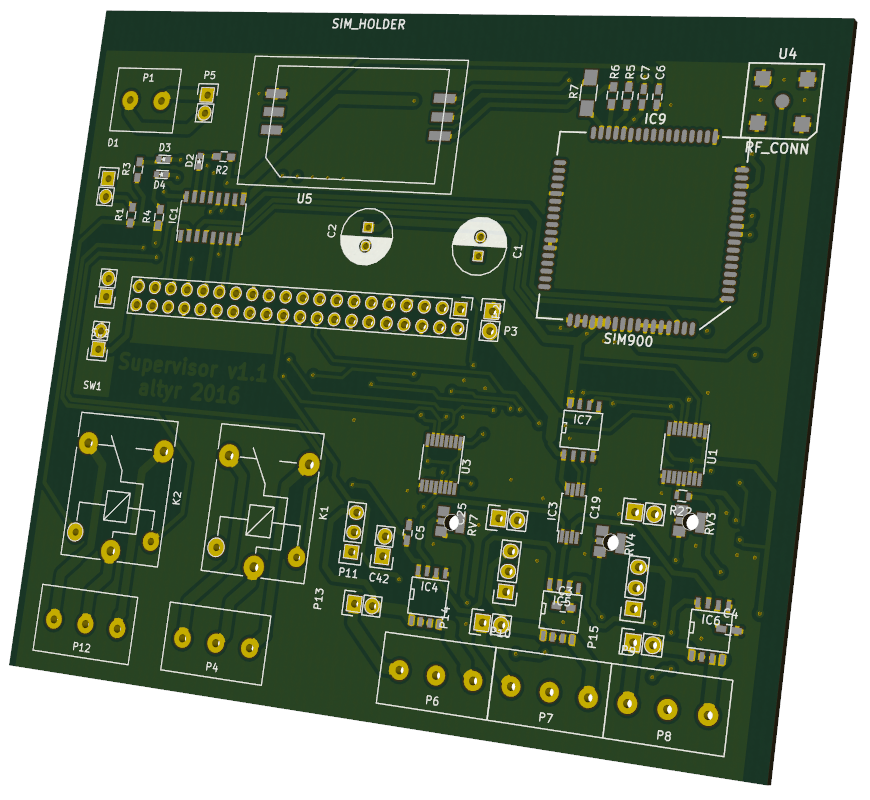
\includegraphics[width=0.9\textwidth]{images/superv-pcb/supervisor-3d-1.png}
            \figcaption[\Master: Vorderseite PCB]{PCB, Vorderseite}
            \label{fig:master:pcb:front}
        \end{minipage}}
        \adjustbox{valign=t}{\begin{minipage}{0.475\textwidth}
            \centering
            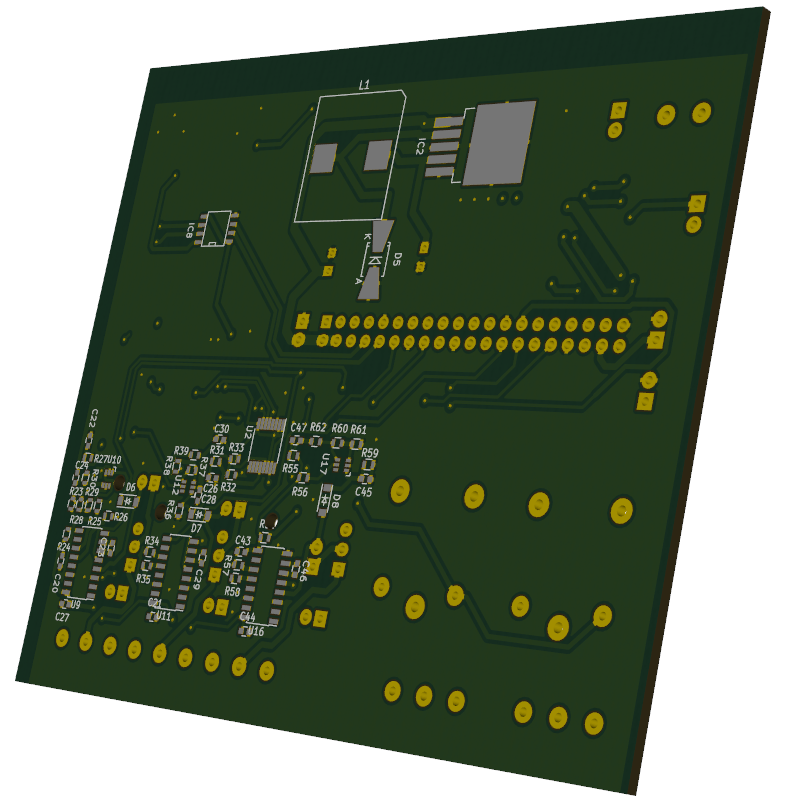
\includegraphics[width=0.9\textwidth]{images/superv-pcb/supervisor-3d-2.png}
            \figcaption[\Master: R\"uckseite PCB]{PCB, R\"uckseite}
            \label{fig:master:pcb:back}
        \end{minipage}}
    \end{minipage}}
    \hspace*{15mm}
    \adjustbox{valign=t}{\begin{minipage}{195mm}

        \centering
        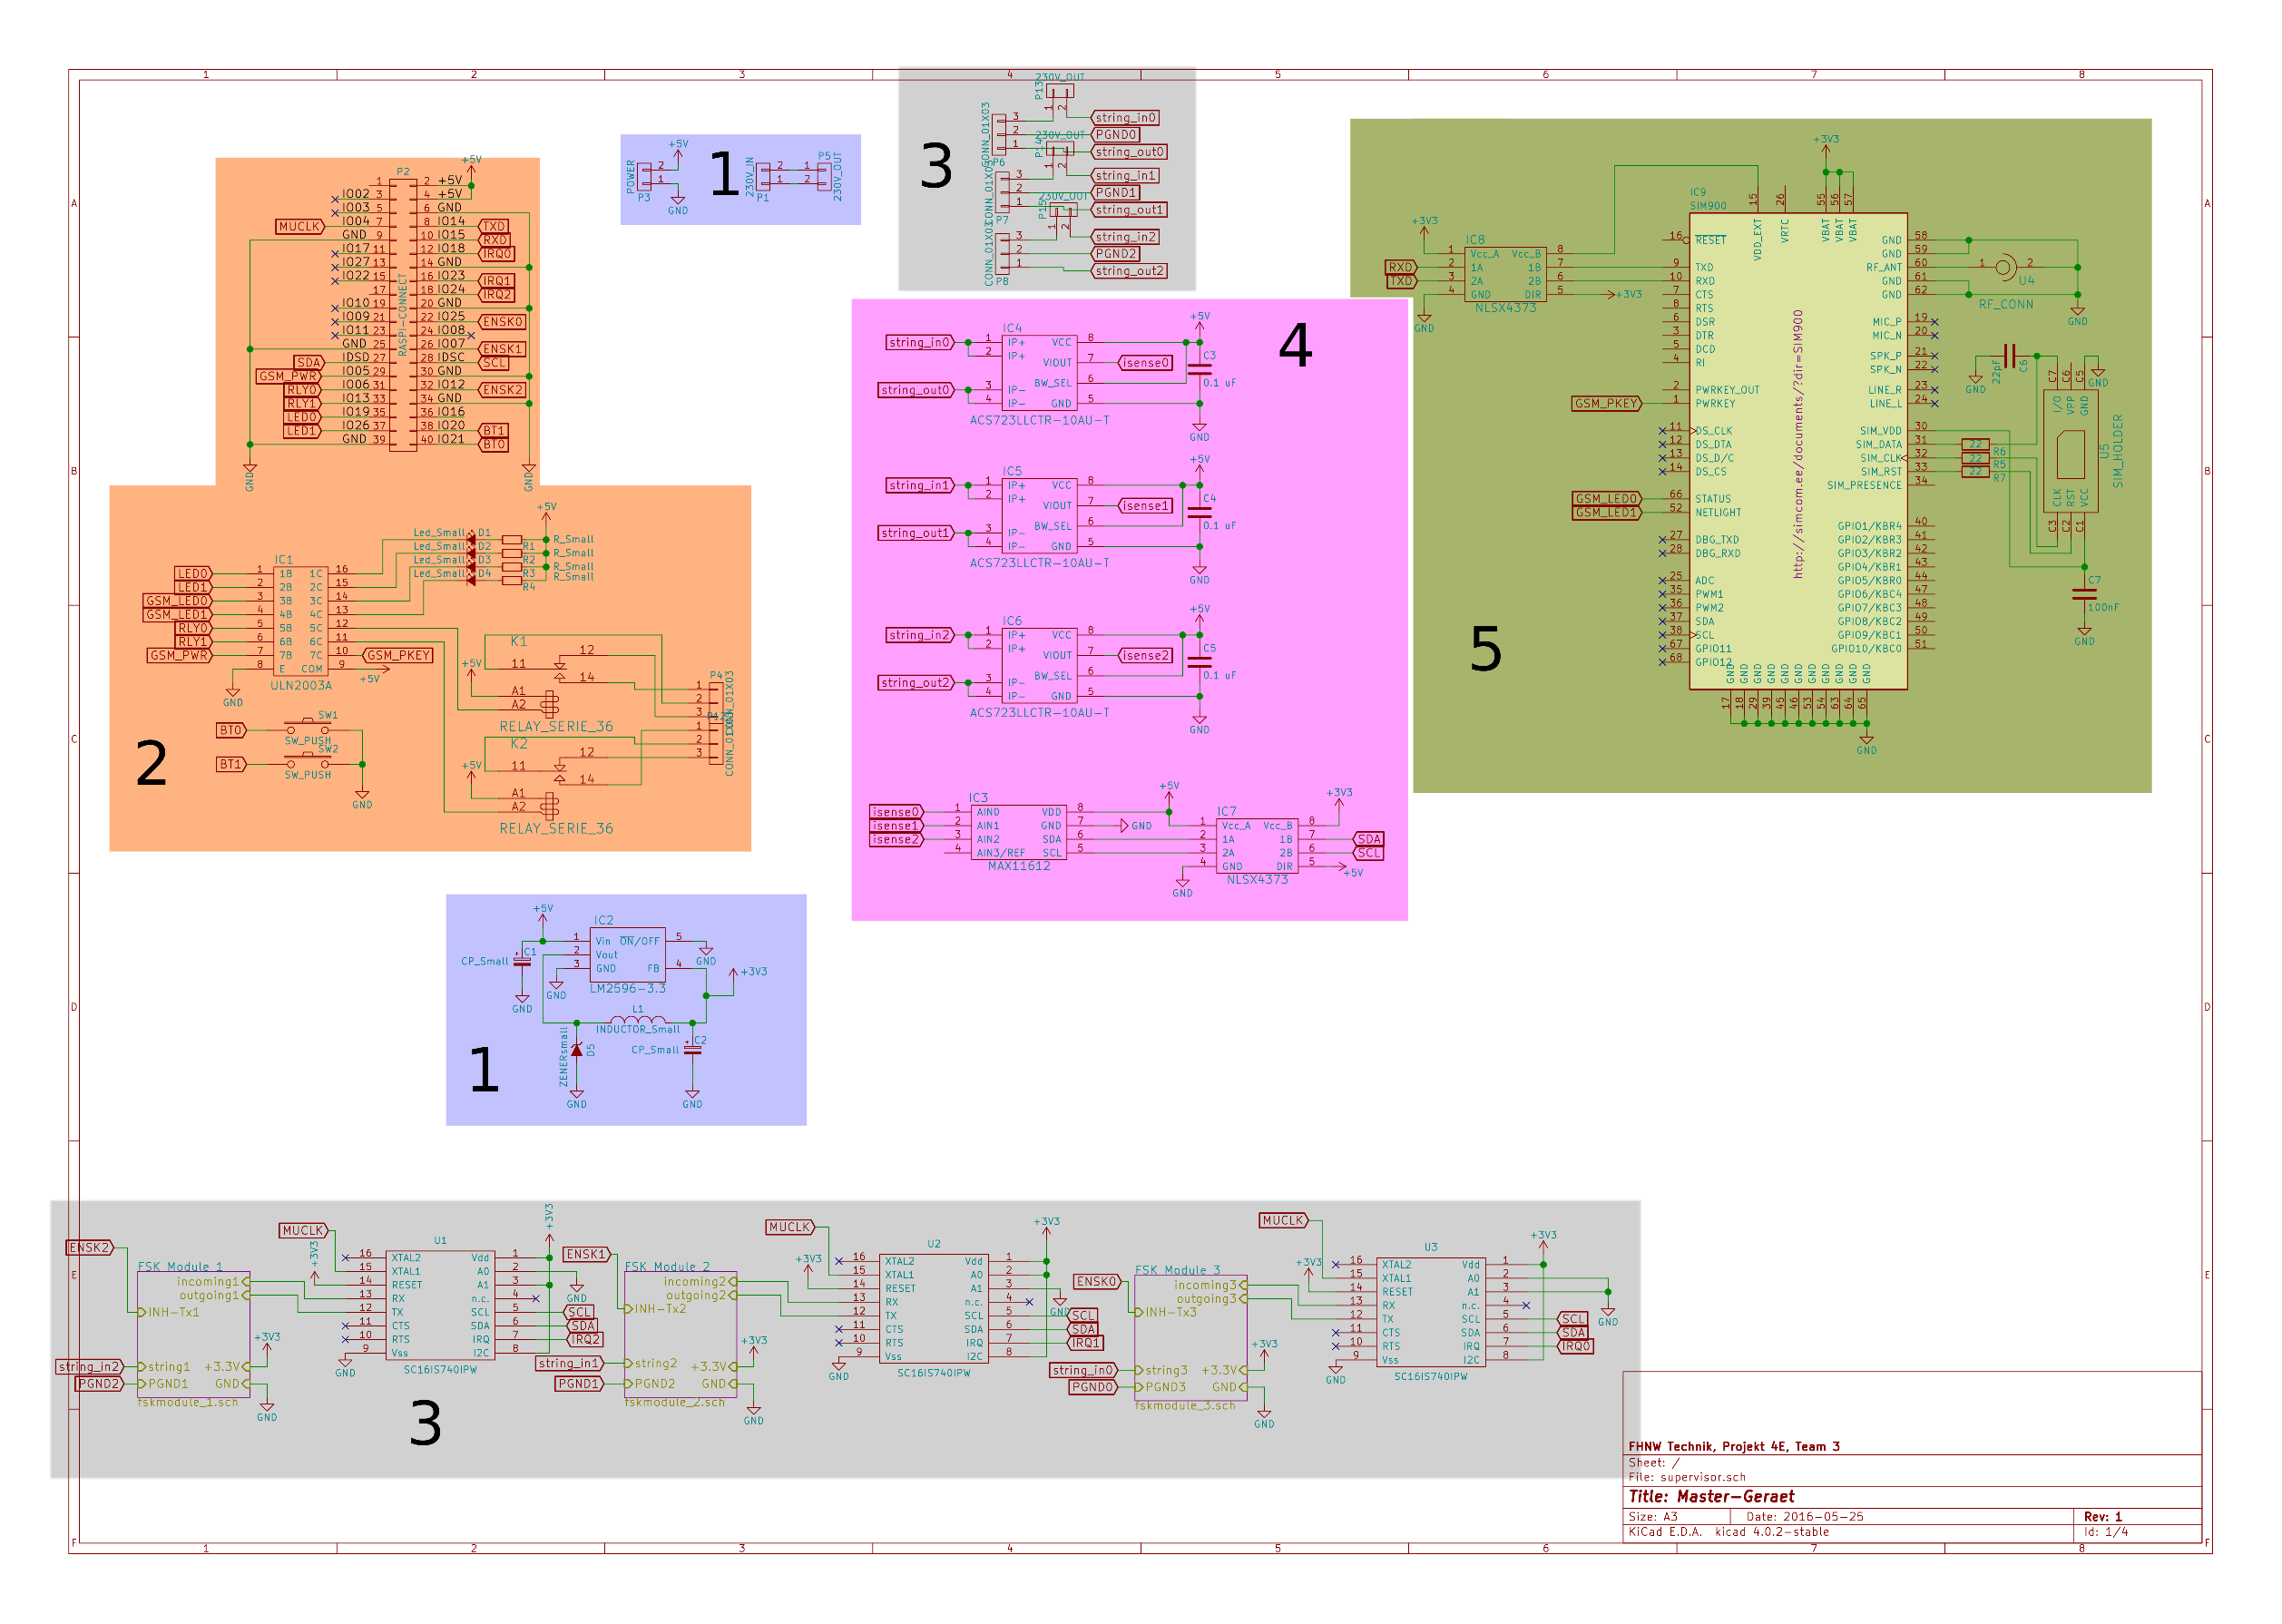
\includegraphics[width=\textwidth]{images/superv-sch/supervisor--sch--highlights.eps}%
        \figcaption[\Master: Schema, \"Ubersicht]{%
            Schema  des  Master-Ger\"ats. Eine   Grossversion  ist  in  Anhang
            \label{app:chap:schemas}  zu  finden,   die  einzelnen  Baugruppen
            sind  in  den  folgenden  Abschnitten  beschrieben  und  gr\"osser
            abgebildet.%
        }
        \label{fig:master:schema:highlights}

    \end{minipage}}
\end{a3pages}}


% ---------------------------------------------------------------------------- %
\subsection{Speisung}
\label{subsec:hw:master:supply}
% ---------------------------------------------------------------------------- %

\begin{figure}[h!t]
    \centering
    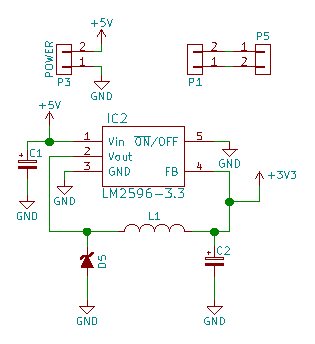
\includegraphics[width=0.33\textwidth]{images/superv-sch/supervisor--sch--supply.eps}
    \caption[\Master: Schema Stromversorgung]{Stromversorgung \Master}
    \label{fig:sch:master:supply}
\end{figure}

Die  Energie wird  vom  \SI{230}{\volt}-Netz bezogen  und  von einem  externen
Netzteil auf \SI{5}{\volt} transformiert. Aus  Platzgr\"unden und aufgrund der
Form  des Geh\"auses  wird der  Netzanschluss dabei  zuerst auf  das PCB  hin-
und  anschliessend zum  Netzger\"at  weggef\"uhrt. Das  Netzteil liefert  dann
\SI{5}{\volt} zur\"uck.

F\"ur  Bauteile, welche  \SI{3.3}{\volt} Versorgungsspannung  ben\"otigen, ist
eine  Spannungswandlung  mit   einem  Schaltregler  implementiert  (\code{IC2}
und  zugeh\"orige Komponenten  in Abbildung  \ref{fig:sch:master:supply}). Der
Schaltregler  ist  das  \SI{3.3}{\volt}-Modell   des  LM2596  von  \emph{Texas
Instruments}.

Hauptverbraucher   auf   der   \SI{3.3}{\volt}-Schiene   ist   das   GSM-Modem
(siehe     Abschnitt     \ref{subsec:hw:master:gsm}),     welches     gem\"ass
Datenblatt~\cite{ref:sim900:1}~bis   zu    \SI{2}{\ampere}   bezieht. Es   ist
daher  wichtig,  dass   die  Spannungsversorgung  der  \SI{3.3}{\volt}-Schiene
gen\"ugend  Strom  liefern  kann. Der  ausgew\"ahlte  Regler  kann  bei  einer
Versorgungsspanunung   von  \SI{5}{\volt}   und  einer   Ausgangsspannung  von
\SI{3.3}{\volt} bis  zu \SI{3}{\ampere} liefern,  was f\"ur das Modem  und die
restlichen Kompomenten auf der \SI{3.3}{\volt}-Linie ausreichen sollte.

Die  Schaltregler  der  LM2596-Linie  integrieren  so  viele  Komponenten  wie
m\"oglich. Dadurch  sind  nur  vier  diskrete  Bauteile  n\"otig,  welche  zur
Unterdr\"uckung  von  Spannungsrippel  ben\"otigt  werden  und  nicht  in  das
Chipgeh\"ause  passen. Sie  werden  anhand   der  Empfehlungen  im  Datenblatt
\cite{ref:lm2596} ausgew\"ahlt:

\begin{itemize}
    \tightlist
    \item
        Spule \code{L1}: \SI{22}{\micro\henry}, Seite 23
    \item
        \code{Cout}: \SI{560}{\micro\farad}, Seite 23
    \item
        Diode \code{D5}: Kompatibel mit SK3-Serie, Seite 24
    \item
        \code{Cin}: \SI{680}{\micro\farad}, Seite 25
\end{itemize}

Tabelle  \ref{tab:hw:master:supply:consumption}  listet die  haupts\"achlichen
Leistungsverbraucher  auf, mit  den Bedingungen,  unter denen  dieser maximale
Verbrauch auftreten kann.

\begin{table}[h!tb]
    \caption{Haupts\"achliche Leistungsverbraucher}
    \label{tab:hw:master:supply:consumption}
    \small
    \begin{tabular}{llll}
        \toprule
        \textbf{Bauteil} & \textbf{Maximale Leistung} & \textbf{Testbedingungen} & \textbf{Quelle} \\
        \midrule
        Raspberry Pi & \SI{4}{W}    & Maximallast im normalen Betrieb  & \cite{ref:raspipower} \\
        Display      & \SI{1.1}{W}  & Maximale Helligkeit              & \cite{datasheet:display} \\
        Modem        & \SI{6.6}{W}  & Alle Kommunikationskan\"ale aktiv  & \cite{ref:modemrefdesign} \\
        Relais       & \SI{0.72}{W} & Zwei Relais, schaltend           & \cite{datasheet:finder36relais} \\
        \bottomrule
    \end{tabular}
\end{table}

Anhand  der  Absch\"atzung  des  Leistungsverbrauchs  wird  als  Netzteil  ein
TXM  025-105  von   \emph{Traco  Power}  ausgew\"ahlt  \cite{ref:farnell:psu}.
Es   handelt    sich   dabei   um   ein    kompaktes   und   kosteng\"unstiges
\SI{5}{\volt}-Netzteil, welches  bis zu \SI{5}{\ampere} liefert  und damit die
Anforderungen gut erf\"ullt.


% ---------------------------------------------------------------------------- %
\subsection{Ein-/Ausg\"ange (GPIO)}
\label{subsec:hw:master:gpio}
% ---------------------------------------------------------------------------- %

\begin{figure}[h!t]
    \centering
    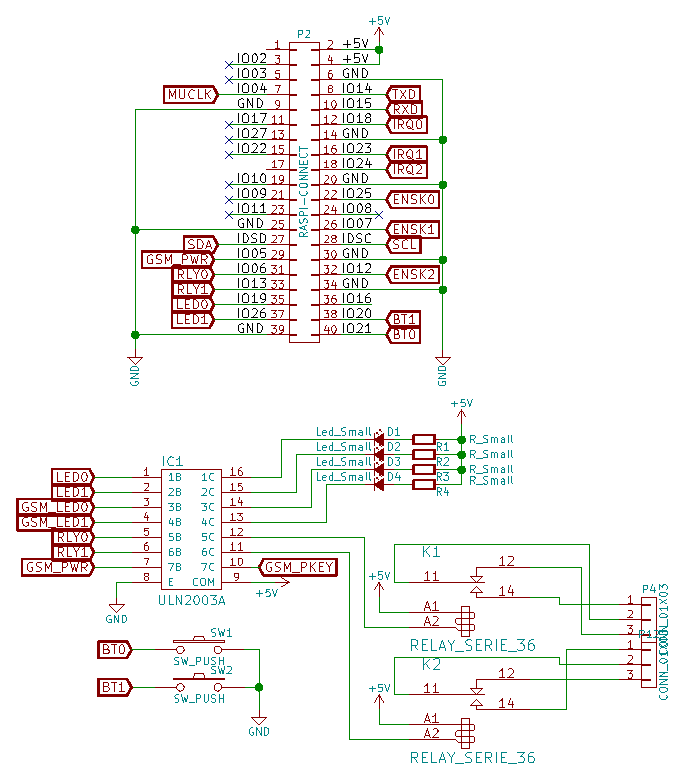
\includegraphics[width=0.725\textwidth]{images/superv-sch/supervisor--sch--gpio.eps}
    \caption[\Master: Schema GPIO]{GPIO \Master}
    \label{fig:sch:master:gpio}
\end{figure}

Das  \Master~  besitzt  verschiedene  Ein-  und   Ausg\"ange. Kernst\"uck  des
GPIO-Blocks  ist  ein Darlington  Transistor  Array  (\code{IC1} in  Abbildung
\ref{fig:sch:master:gpio}),  welches verschiedene  Steuersignale durchschalten
kann.

Die  Signale  \code{LED0}  und  \code{LED1} steuern  die  LEDs  \code{D1}  und
\code{D2},   werden  vom   \Raspi~  gesteuert   und  dienen   dem  allgemeinen
Debugging. Signal  \code{GSM\_LED0}  respektive  \code{GSM\_LED1}  stehen  dem
GSM-Modem zur Statusausgabe zur Verf\"ugung.

Die   beiden  Relais   werden  von   \code{RLY0}  und   \code{RLY1}  gesteuert
und  k\"onnen  vom  Endbenutzer   f\"ur  beliebige  Funtionalit\"at  verwendet
werden. Daf\"ur stehen  die beiden  Anschl\"usse \code{P4} und  \code{P16} zur
Verf\"ugung.

Das Signal \code{GSM\_PWR} kann auf \code{GND} durchschalten, um das GSM-Modem
via den Pin  \code{GSM\_PKEY} einzuschalten, analog zu einem  Taster, um einen
PC einzuschalten.

Die  beiden  Anschl\"usse  \code{BT0}  und \code{BT1}  sind  mit  dem  \Raspi~
verbunden und k\"onnen f\"ur Jumper, Taster oder Schalter verwendet werden. In
der  Prototypenkonfiguration  ist   ein  Schalter  angeschlossen. Der  Stecker
\code{P2} ist die Hauptverbindung zum \Raspi~via Flachbandkabel.

Als  IO-Verst\"arker  wird  ein   ULN2003A  von  Texas  Instruments  gew\"ahlt
\cite{datasheet:darlingtonic}. Der    IC    verf\"ugt    \"uber    integrierte
Freilaufdioden   zum    Schutz   vor    \"uberh\"ohter   Spannung    auf   der
Ausgangsseite. In unserem Fall dient  dies dazu, Spannungsspitzen, welche beim
Ausschalten der Relais auftreten k\"onnen,  abzufangen.  Da der \Raspi~maximal
\SI{3.3}{\volt} am  Ausgang liefern  kann, muss  die Schaltschwelle  f\"ur ein
\code{true}-Signal bei diesem  IC bei \SI{3.3}{\volt} oder  tiefer liegen, was
der  ULN2003A erf\"ullt.   Die Relais  beziehen bis  zu \SI{72}{\milli\ampere}
\cite{datasheet:finder36relais}  Strom  bei   Betrieb  mit  \SI{5}{\volt}. Der
ULN2003A kann bis zu \SI{100}{\milli\ampere} pro Kanal liefern, was ausreichen
sollte, um die Relais zuverl\"assig schalten zu k\"onnen.

Die     Relais      sind     von      der     Serie     36      von     Finder
\cite{datasheet:finder36relais}. Sie  k\"onnen Lasten  bis zu  \SI{230}{\volt}
und  \SI{10}{\ampere}  schalten,  womit handels\"ubliche  Ger\"ate  f\"ur  das
Niederspannungsnetz angeschlossen werden k\"onnen. Dies gibt dem Kunden grosse
Flexibilit\"at bei der Wahl der  zu betreibenden Ger\"ate (Alarmlampe, Sirene,
\ldots).


% ---------------------------------------------------------------------------- %
\subsection{Kommunikation mit Sensoren}
\label{subsec:hw:master:sensorcomm}
% ---------------------------------------------------------------------------- %


\begin{figure}[h!t]
    \centering
    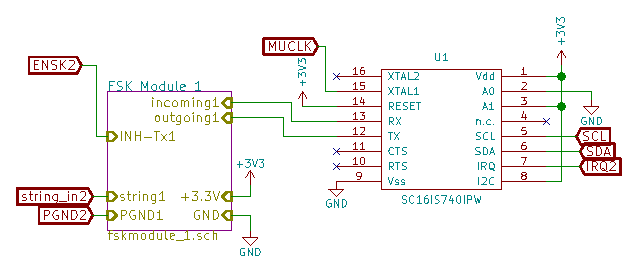
\includegraphics[width=0.75\textwidth]{images/superv-sch/supervisor--sch--comms.eps}
    \caption[\Master: Schema Kommunikation]{Kommunikation zu \Sensor~auf \Master}
    \label{fig:sch:master:comms}
\end{figure}

Abbildung     \ref{fig:sch:master:comms}     zeigt    das     Schema     einer
der    drei     Schaltungen,    welche     zur    Kommunikation     mit    dem
Sensor    benutzt     werden. Zur    genauen    Beschreibung     des    Blocks
\code{fskmodule\_1.sch} siehe Abschnitt \ref{subsec:hw:sensor:transmitter} auf
Seite \pageref{subsec:hw:sensor:transmitter}.

Auf der rechten Seite in Abbildung \ref{fig:sch:master:comms} ist die Br\"ucke
\code{U1} abgebildet,  welche zwischen UART und  \ISC~konvertiert. Es wird das
Modell  SC16IS740 von  NXP Semiconductors  \cite{datasheet:uarti2c} verwendet.
Der \Sensor~ sendet seine Daten  auf der DC-Leitung in  UART-Kodierung. Da der
\Raspi~nicht  gen\"ugend  UART-Eing\"ange  f\"ur alle  ben\"otigten  Leitungen
besitzt,  werden  die  Daten  im \ISC-Format  in  den  \Raspi~eingespeist. Die
Br\"ucke  \code{U1} ist  daf\"ur verantwortlich,  zwischen UART  (Anschl\"usse
\code{TX}  und \code{RX}  und  \ISC~(Anschl\"usse \code{SDA}  f\"ur Daten  und
\code{SDL} f\"ur Clock) zu konvertieren.

Den Clock erh\"alt die Br\"ucke vom Mikrocontroller des \Raspi~via die Leitung
\code{MUCLK}.

Wenn  von einem  \Sensor~Daten  empfangen werden,  kann die  Br\"ucke mit  dem
Anschluss \code{IRQ2} einen Interrupt an den \Raspi~senden, welcher darauf die
Datenverarbeitung startet.

Die Pins  \code{A0} und  \code{A1} dienen der  Addressierung der  Br\"ucke und
sind f\"ur  jede Br\"ucke individuell angeschlossen. F\"ur  die vollst\"andige
Verdrahtung  siehe Seite
\pageref{fig:schema:master:full}
in Anhang
\ref{app:chap:schemas}

\fref{fig:sch:master:coupling}  zeigt  die  Anschl\"usse zur  Einkopplung  des
Signals  auf  die  DC-Leitung. Es  sind drei  Stecker  \code{P13},  \code{P14}
und  \code{P15}  vorhanden,  durch  welche der  Strom  geleitet  wird. An  den
Steckern  kann jeweils  eine  Einkopplung  angeschlossen werden. Dies  erlaubt
Flexibilit\"at bei der  Implementierung der Einkopplung, da das  PCB nicht auf
eine spezifische Variante beschr\"ankt ist.

Die Ausg\"ange des Einkopplungsblocks gehen auf die Strommessung.
\begin{figure}[h!tb]
    \centering
    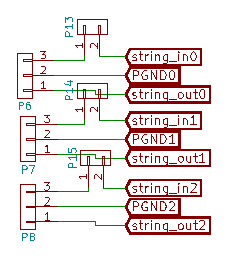
\includegraphics[width=0.25\textwidth]{images/superv-sch/supervisor--sch--coupling.eps}
    \caption[\Master: Schema Einkopplung]{Anschl\"usse zur Einkopplung}
    \label{fig:sch:master:coupling}
\end{figure}


% ---------------------------------------------------------------------------- %
\subsection{Strommessung}
\label{subsec:hw:master:current}
% ---------------------------------------------------------------------------- %


\begin{figure}[h!t]
    \centering
    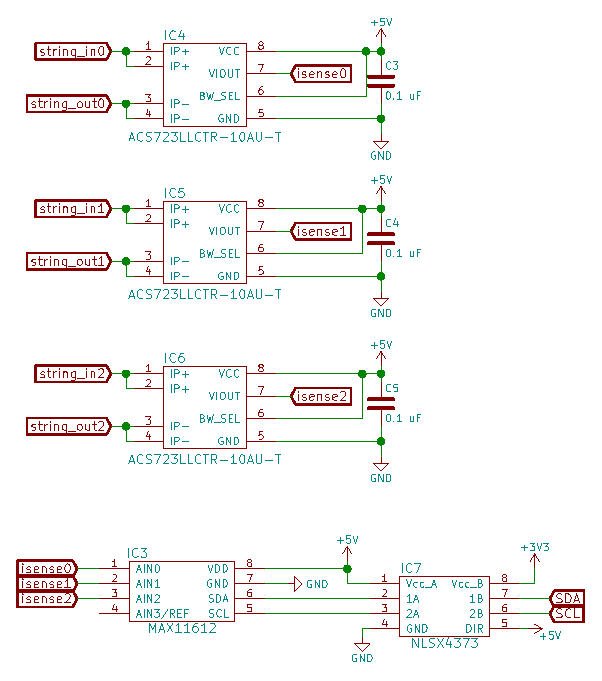
\includegraphics[angle=-90,width=0.60\textwidth]{images/superv-sch/supervisor--sch--current.eps}
    \caption[\Master: Schema Strommessung]{Strommessung}
    \label{fig:sch:master:current}
\end{figure}

Der  Strom jedes  Modulstrangs  wird separat  \"uberwacht;  die dazu  benutzte
Schaltung   ist   in   Abbildung   \ref{fig:sch:master:current}   dargestellt.
\code{IC4},  \code{IC5}  und  \code{IC6}  sind  die  Strommessungssensoren. Es
werden  Hall-Sensoren   der  Modellreihe   ACS725  von   Allegro  Microsystems
benutzt. Diese k\"onnen bis zu  \SI{10}{\ampere} messen, sind durchschlagsfest
bis zu  \SI{2.5}{\kilo\volt} (Mindestanforderung  \SI{1}{\kilo\volt}, Spannung
auf  einer  DC-Leitung)  und  k\"onnen sowohl  mit  \SI{3.3}{\volt}  wie  auch
\SI{5}{\volt} betrieben werden \cite{datasheet:hallic}.

Sie  geben   auf  den  Leitungen  \code{isense0},   \code{isense1}  respektive
\code{isense2}  eine   Spannung  aus,  welche  proportional   zum  den  Sensor
durchfliessenden Strom ist. Der vom Modulstrang  kommende Strom geht in in die
Eing\"ange \code{string\_in\{0,1,2\}} der Sensoren und verl\"asst diese wieder
durch die Ausg\"ange \code{string\_out\{0,1,2\}}, von  wo er weitergeht in den
Generatoranschlusskasten.

\code{IC3}   ist    der   A/D-Konverter,   welcher   die    analogen   Signale
\code{isense0} bis \code{isense2} in  digitale Signale mit \SI{5}{\volt}-Pegel
wandelt. Es   kommt   ein   MAX11612   von  Maxim   Integrated   zum   Einsatz
\cite{datasheet:adc}. Dieser besitzt ein \ISC-Interface, drei Kan\"ale und ist
mit  dem  Ausgangspegel  der  Hall-Sensoren  kompatibel.   Allerdings  liefert
er  ein  Ausgangssignal  mit  einem \SI{5}{\volt}-Pegel,  was  nicht  mit  dem
\Raspi~ kompatibel ist, dessen Eing\"ange  mit einem Pegel von \SI{3.3}{\volt}
laufen. Deshalb wird zwischen \code{IC3}  und dem \Raspi~noch ein Pegelwandler
der   Serie   NLSX4373  von   ON   Semiconductors   geschaltet,  welcher   das
\SI{5}{\volt}-Signal des ADC auf  \SI{3.3}{\volt} konvertiert. Er ist speziell
f\"ur  \ISC-Anwendungen entwickelt  worden  und eignet  sich  somit gut  f\"ur
unsere Zwecke.

Der Hersteller sieht zur  Stabilisierung der Stromversorgung einen Kondensator
der  Gr\"osse \SI{100}{\nano\farad},  sichtbar  im Diagramm  auf  Seite 1  des
Datenblattes \cite{datasheet:hallic}, vor.

% ---------------------------------------------------------------------------- %
\clearpage
\subsection{GSM-Modem}
\label{subsec:hw:master:gsm}
% ---------------------------------------------------------------------------- %

\begin{figure}[h!t]
    \centering
    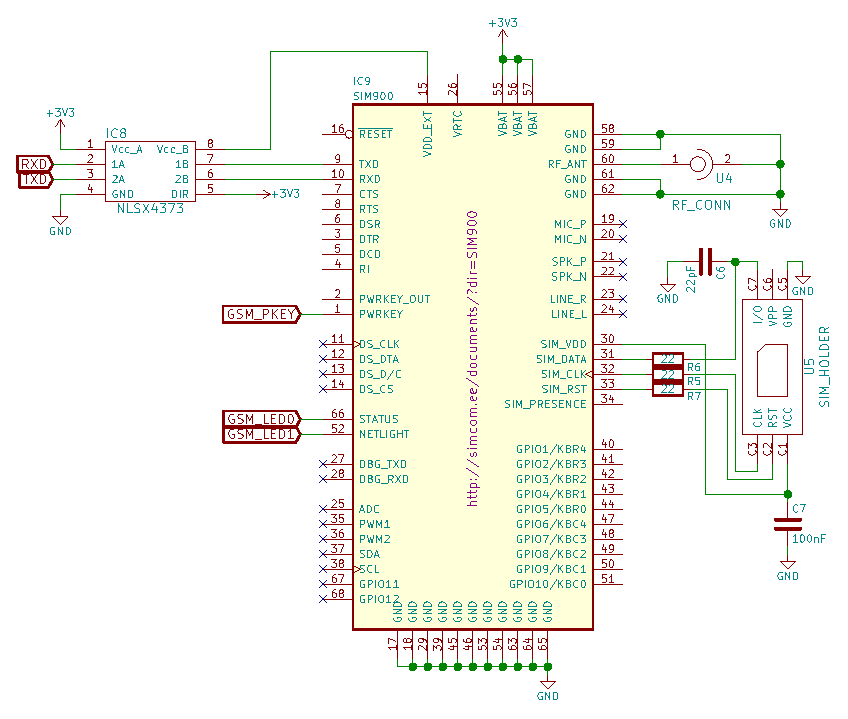
\includegraphics[width=0.85\textwidth]{images/superv-sch/supervisor--sch--gsm.eps}
    \caption[\Master: Schema GSM-Modem]{GSM-Modem Schaltung}
    \label{fig:sch:master:gsm}
\end{figure}

Das   GSM-Modem   ist   ein   integrierter  Baustein,   der   alle   n\"otigen
Funktionen  bereitstellt. Es  wird  ein  Modell der  SIM900-Serie  von  Simcom
\cite{datasheet:modem}  verwendet.  Das  Modem und  seine Beschaltung  sind in
Abbildung \ref{fig:sch:master:gsm} dargestellt. Wie  auch bei der Strommessung
wird  hier  ein   Pegelwandler  verwendet,  um   das  Signal   von  der
UART-Linie mit  \SI{3.3}{\volt} auf  den vom  GSM-Chip ben\"otigten  Pegel von
\SI{2.8}{\volt} (Pin \code{VDD\_EXT} auf dem Chip, verbunden mit \code{Vcc\_B}
auf dem Pegelwandler) zu wandeln.

Der  Pin  \code{GSM\_PKEY} dient  zum  Einschalten  des GSM-Modems,  gesteuert
vom  \Raspi~ via  GPIO  (siehe  Abschnitt  \ref{subsec:hw:master:gpio},  Seite
\pageref{subsec:hw:master:gpio}).

Via die beiden Pins \code{STATUS}  und \code{NETLIGHT} werden zwei Status-LEDs
angesteuert (siehe  ebenfalls Abschnitt  \ref{subsec:hw:master:gpio}). Auf der
rechten Seite des Schaltungsblocks sind die  Antenne und der Adapter f\"ur die
SIM-Karte zu sehen.

Gem\"ass  Referenzdesign  auf  Seite 9  des  Modem-Guides  \cite{ref:sim900:1}
betr\"agt der Wert aller Simkarten-Widerst\"ande \SI{22}{\ohm}.

% **************************************************************************** %
\chapter{Software}
\label{chap:software}
% **************************************************************************** %

Die  Software   unseres  Systems   gliedert  sich   analog  zur   Hardware  in
zwei  prim\"are  Teile: Die   Firmware  des  Sensors  und   die  Software  des
Masters.

In  Abschnitt  \ref{sec:fw:dataFlow} wird  im  Folgenden  kurz dargelegt,  wie
diese beiden  Teilsysteme verkn\"upft sind. Anschliessend  erkl\"art Abschnitt
\ref{sec:firmware:sensor}  die Funktionsweise  der  Firmware des  Sensors. Die
Software des \Raspi~ ist  abschliessend in Abschnitt \ref{sec:software:master}
dokumentiert.


{\begin{a3pages}
\setlength{\parindentbak}{\parindent}
    \noindent\adjustbox{valign=t}{\begin{minipage}{115mm}
    % ---------------------------------------------------------------------------- %
    \section{Datenfluss}
    \label{sec:fw:dataFlow}
    % ---------------------------------------------------------------------------- %
    Abbildung  \ref{fig:dataFlow}   zeigt  den   Ablauf  der   Spannungs-  und
    Strommessung von den Messsonden bis zur Speicherung der Messergebnisse und
    der zugeh\"origen Metadaten in der Datenbank.

    \setlength{\parindent}{\parindentbak}  %   restore  paragraph  indentation
    Die   Spannung  wird   in  jedem   PV-Modul  von   einem  Sensor   mittels
    eines    analog/digital-Konverters   gemessen. Anschliessend    wird   ein
    laufender  Durchschnittswert  (siehe  Abschnitt  \ref{subs:Sensor},  Seite
    \pageref{subs:Sensor})  zusammen mit  der Serienummer  des Microchips  und
    einer  Checksumme in  ein  Datenpaket gepackt  und  \"uber die  DC-Leitung
    verschickt.

    Die   ON-OFF    Keying-Schaltung   benutzt   als   Referenz    den   Clock
    eines     separaten,     spannungsgesteuerten    Oszillators     (englisch
    \emph{voltage-controlled oscillator}, VCO).

    Im  \Master~  wird das  Datenpaket  entpackt  und auf  seine  Integrit\"at
    gepr\"uft.   Passt die  Pr\"ufsumme nicht  zu  den Daten,  wird das  Paket
    verworfen. Sind  die Daten  intakt  (bzw. wird  keine Diskrepanz  zwischen
    Pr\"ufsumme und  Daten festgestellt),  werden Spannung und  Serienummer im
    zugeh\"origen Table der Datenbank gespeichert. Zur chronologischen Ordnung
    der Daten wird  noch ein Timestamp abgelegt. Damit man  weiss, aus welchem
    Strang das Paket gekommen ist, wird  die Strang-Nummer noch in den Eintrag
    eingef\"ugt.

    Die  Messung der  Strang-Str\"ome  erfolgt direkt  vom  \Master~ aus;  die
    zugeh\"origen Messwerte werden in einem separaten Table abgelegt.

    Zur  Verwaltung  der  installierten  Sensoren  und  PV-Module  wird  f\"ur
    jeden  Strang  ein  Table  gef\"uhrt,  in  dem  die  Serienummern  der  in
    diesem Strang  installierten Sensoren (bzw. deren  Microchips) gespeichert
    sind. Die  Eintr\"age  in  diesen  Tables erfolgen  automatisch,  wenn  in
    einem ankommenden  Datenpaket eine bisher noch  nicht bekannte Serienummer
    detektiert wird.

    \vspace*{40mm}

    \hfill\adjustbox{valign=t}{\begin{minipage}{50mm}
        \figcaption
        [Datenfluss von Messungen bis Speicherung]
        {%
            Datenfluss von den Messungen der Modulspannungen und Strang-Str\"ome bis
            zur Speicherung in der Datenbank%
        }
        \label{fig:dataFlow}
    \end{minipage}}
\end{minipage}}
\hspace*{15mm}
\adjustbox{valign=t}{\begin{minipage}{215mm}
    \begin{tikzpicture}[%
        align=center,
        text=solarized-base02,
        draw=solarized-base02,
        remember picture,
        overlay,
    ]
    \small
    \sffamily
    %\begin{scope}[x={(0mm,0.95\textwidth)},y={(0mm,50mm)}]

    %\draw [help lines] (0,0) grid (10,-15);

    \begin{scope}[
        every node/.style = draw,
        terminal/.append style={
            rounded rectangle,
            fill=solarized-violet,
            text=solarized-base3,
            inner sep=2mm,
        }, % data packages
        sign/.style={
            inner sep=2mm,
            rounded corners=1mm,
            fill=solarized-magenta,
            text=solarized-base3,
        },         % custom signal style
        circ/.style={
            inner sep=2mm,
            rounded corners=1mm,
            double,
            fill=solarized-base02,
            draw=solarized-base02,
            text=solarized-base2,
        }, % circuitry
        proc/.style={
            inner sep=2mm,
            rounded corners=1mm,
            fill=solarized-cyan,
            text=solarized-base3,
        },       % process/activity
        stor/.style={
            fill=cyan!30
        },         % storage
        dbtable/.style={
            text=solarized-base3,
            draw=solarized-base3,
            rounded corners=1mm,
            inner sep=2mm,
        } % database tables
    ]
        \node (voltage) [
            sign,
            signal,
            signal to=east
        ] at (20mm,-33mm) {Spannung};

        % uC on Sensor
        \node (ADCVolt) [
            circ,
            right=30mm of voltage
        ] {ADC};
        \node (avg) [
            proc,
            right=of ADCVolt,
            align=center
        ] {Durchschnitt\\berechnen};
        \node (data) [
            terminal,
            right=of avg,
            align=center
        ] {Messdaten\\Modulspannung,\\Sensor-ID};
        \node (id) [
            sign,
            signal,
            signal to=east,
            above left=of data
        ] {Seriennummer};
        \node (crc) [
            proc,
            below right=of data
        ] {CRC berechnen};
        \node (package) [
            terminal,
            below=of data
        ] {Datenpaket};
        \node (uart) [
            circ,
            left=of package
        ] {UART-Modul};

        \node (oosk1)[
            circ,
            below left=of uart,
            align=center
        ] {ON/OFF-Shift \\Keying-Schaltung};
        \node (clk1) [
            sign,
            signal,
            signal to=west,
            right=2cm of oosk1
        ] {CLK VCO};
        \node (oosk2) [
            circ,
            below=20mm of oosk1,
            align=center
        ] {ON/OFF-Shift \\Keying-Schaltung};
        \node (clk2) [
            sign,
            signal,
            signal to=east,
            left=2cm of oosk2
        ] {CLK VCO};
        \node (bridge) [
            circ,
            right=of oosk2
        ] {UART/I\textsuperscript{2}C-Br\"ucke};
        \node (package2) [
            terminal,
            right=of bridge
        ] {Datenpaket};

        % Raspi
        \node (crc2) [
            proc,
            align=center,
            diamond,
            below=of package2
        ] {CRC\\korrekt?};
        \node (discard) [
            draw=solarized-red,
            cross out,
            right=of crc2
        ] {Paket verwerfen};
        \node (data2) [
            terminal,
            left=of crc2,
            align=center
        ] {Messdaten\\Modulspannung,\\Sensor-ID};
        \node (dbVolts) [
            dbtable,
            left=of data2,
            text width=7em,
            align=left,
            minimum width=7.5em
        ] {Table:\\ Spannungen\\};
        \node (dbCurr) [
            dbtable,
            below=1mm of dbVolts,
            text width=7em,
            align=left,
            minimum width=7.5em
        ] {Table:\\ Strang-Str\"ome\\};
        \node (dbIDs) [
            dbtable,
            below=1mm of dbCurr,
            text width=7em,
            align=left,
            minimum width=7.5em
        ] {Tables:\\ Sensor-IDs \\ pro Strang};

        \node (newID) [
            proc,
            align=center,
            diamond,
            below=of crc2] {Sensor-ID\\bekannt?};
        \node (sensorID)  [
            terminal,
            left=of newID] {Sensor-ID};
        \node (stringNr2) [
            sign,
            signal,
            signal to=west,
            below=5mm of sensorID
        ] {String-Nr.};

        \node (stringNr) [
            sign,
            signal,
            signal to=east,
            left=15mm of dbVolts
        ] {String-Nr.};
        \node (timestamp) [
            sign,
            signal,
            signal to=east,
            above=1mm of stringNr
        ] {Timestamp};

        \node (dataCurr) [
            terminal,
            below=35mm of stringNr,
            align=center
        ] {Messdaten\\Strom};

        \node (bridge2) [
            circ,
            below=60mm of stringNr
        ] {UART/I\textsuperscript{2}C-Br\"ucke};
        \node (hall) [
            circ,
            right=of bridge2
        ] {Hall-Sensoren};
        \node (current) [
            sign,
            signal,
            signal to=west,
            below right=of hall
        ] {Strang-Strom};
    \end{scope}

    \begin{scope}
        % Need to have this inside  a separate scope so that
        % its border does not get drawn.
        \node (db)        [
            text=solarized-base3,
            above=1mm of dbVolts,
            align=left
        ] {Datenbank};
        \node (dbSignals) [
            circle,
            inner sep=1pt,
            fill=solarized-base03,
            right=3mm of stringNr
        ] { };
        \node (dbSignals2) [
            circle,
            inner sep=1pt,
            fill=solarized-base03,
            left=4mm of dbCurr] { };
        \node (dbSignals3) [
            circle,
            inner sep=1pt,
            fill=solarized-base03,
            left=of sensorID
        ] { };
    \end{scope}

    \begin{scope}[on background layer]
        \node (SENSOR) [%
            draw,
            double,
            rounded corners=5mm,
            fill=solarized-base3,
            inner sep=2em,
            fit=(ADCVolt) (avg) (data) (id) (crc) (package) (uart) (oosk1) (clk1),
            align=left,
            text height=21em,
            align=right,
        ] {\large{\textbf{Sensor}}};
        \node (uCSensor) [%
            draw,
            double,
            rounded corners=5mm,
            fill=solarized-base2,
            inner sep=1em,
            fit=(ADCVolt) (avg) (data) (id) (crc) (package) (uart),
            align=right,
            text height=1em,
        ] {\textbf{Atmel SAM D09}};
        \node (MASTER) [%
            draw,
            double,
            rounded corners=5mm,
            fill=solarized-base3,
            inner sep=2em,
            fit=(clk2) (bridge2) (hall) (stringNr) (timestamp) (crc2) (newID) (discard) (stringNr2),
            align=right,
            text height=1em,
        ] {\large{\textbf{Master}}};
        \node (rasPi) [%
            draw,
            double,
            rounded corners=5mm,
            fill=solarized-base2,
            inner sep=1em,
            fit=(stringNr) (timestamp) (crc2) (newID) (discard) (stringNr2),
            align=right,
            text height=1em,
        ] {\textbf{Raspberry Pi}};
        \node (database) [%
            draw=solarized-base03,
            rounded corners=3mm,
            inner sep=2mm,
            fill=solarized-blue,
            fit=(dbVolts) (dbCurr) (dbIDs) (db),
        ] { };
    \end{scope}


    \begin{scope}[
        %every node/.style={ },
            rounded corners,
            every path/.append style={draw=solarized-base03,},
    ]
        \draw[-latex] (voltage) -- (ADCVolt);
        \draw[-latex] (ADCVolt) -- (avg);
        \draw[-latex] (id) -| (data);
        \draw[-latex] (avg) -- (data);
        \draw[-latex] (data) -| (crc);
        \draw[-latex] (crc) -- (package);
        \draw[-latex] (data) -- (package);
        \draw[-latex] (package) -- (uart);
        \draw[-latex] (uart) -| (oosk1);
        \draw[-latex] (clk1) -- (oosk1);
        \draw[-latex] (clk2) -- (oosk2);
        \draw[line width=2pt,-latex] (oosk1) --  node[midway, anchor = west] {DC-Leitung} (oosk2);
        \draw[-latex] (oosk2) -- (bridge);
        \draw[-latex] (bridge) -- (package2);
        \draw[-latex] (package2) -- (crc2);
        \draw[-latex] (crc2) -- node[anchor=north] {nein} (discard);
        \draw[-latex] (crc2) -- node[anchor=north] {ja} (data2);
        \draw[-latex] (data2) -- (dbVolts);
        \draw[-] (stringNr) -- (dbSignals);
        \draw[-] (timestamp) -| (dbSignals);
        \draw[-latex] (dbSignals) -- (dbVolts);
        \draw[-latex] (dbSignals) -| (dbSignals2);
        \draw[-latex] (dbSignals2) -- (dbCurr);
        \draw[-latex] (crc2) -- node[anchor=west,align=right] {ja} (newID);
        \draw[-latex] (newID) -- node[anchor=north] {nein} (sensorID);
        \draw[-latex] (sensorID) -| (dbIDs);
        \draw[-latex] (stringNr2) -| (dbSignals3);
        \draw[-latex] (current) -| (hall);
        \draw[-latex] (hall) -- (bridge2);
        \draw[-latex] (bridge2) -- (dataCurr);
        \draw[-latex] (dataCurr) |- (dbSignals2);
    \end{scope}

\end{tikzpicture}

\end{minipage}}
\end{a3pages}}

{\begin{a3pages}
% ---------------------------------------------------------------------------- %
\section{Firmware \Sensor}
\label{sec:firmware:sensor}
% ---------------------------------------------------------------------------- %

\setlength{\parindentbak}{\parindent}
    \noindent\adjustbox{valign=t}{\begin{minipage}{135mm}
Als  CPU auf  dem  Sensor agiert  wie im  Abschnitt~\ref{sec:hw:sensorplatine}
erw\"ahnt   ein  Atmel   Smart  ARM   Cortex  M0+.    Die  Firmware   ist  aus
Kompatibilit\"atsgr\"unden zur CPU in C geschrieben.

% ---------------------------------------------------------------------------- %
\subsection{Benutzte Bibliotheken}
% ---------------------------------------------------------------------------- %

Es wird komplett freie Software verwendet, weswegen zum Bauen der Binaries GNU
Makefiles benutzt werden.

    \setlength{\parindent}{\parindentbak} % restore paragraph indentation
Die  Firmware  ist  auf  dem Atmel  Software  Framework  (ASF)  aufgebaut. Das
ASF  f\"uhrt  einen   Hardware  Abstraction  Layer  (HAL)   ein,  welcher  die
Hardware-Bl\"ocke der einzelnen Atmel CPUs  in einfache Interfaces in Form von
C-Funtionen abstrahiert. Um die g\"angigen  ARM-Schnittstellen zu nutzen, wird
CMSIS im  ASF  verwendet. Das  ASF  darf  f\"ur  Atmel  Chips  ohne  weiteres
verwendet werden, solange die Copyright Bemerkungen nicht entfernt werden.

% ---------------------------------------------------------------------------- %
\subsection{Die Firmware}
% ---------------------------------------------------------------------------- %

Die Firmware besteht im Kern aus einer \code{main()}-Funktion, welche in einer
Endlosschleife   l\"auft. Abbildung~\ref{fig:sensor:firmware:mainloop}  zeigt,
wie  diese  Schleife  aufgebaut  ist.  Zudem  zeigt  sie  den  regelm\"assigen
\code{SysTick}-Interrupt, welcher den ADC ausliest und die LEDs toggelt.

% ---------------------------------------------------------------------------- %
\subsubsection{UART}
\label{subs:UART}
% ---------------------------------------------------------------------------- %

Die Endlosschleife  \"uberpr\"uft zuerst, ob  Daten \"uber die  UART empfangen
wurden, sprich Anweisungen vom Master oder Antworten von anderen Sensoren. Ist
das der Fall, so wird darauf reagiert.  Zuerst wird \"uberpr\"uft ob das Paket
auch f\"ur den Sensor bestimmt ist. Falls das  erste Byte 0 ist, ist das Paket
f\"ur den Master bestimmt. Falls es 1 ist, so ist das Paket f\"ur einen Sensor
bestimmt. Um  zu bestimmen,  ob  das  Paket f\"ur  sich  selbst bestimmt  ist,
pr\"uft  die Firmware,  ob  die  n\"achsten 4  empfangenen  Bytes der  eigenen
ID  entsprechen. Hier  ist wichtig,  dass  alle  Daten Little  Endian  codiert
sind.  Falls das Paket tats\"achlich f\"ur  den Sensor bestimmt ist, so wertet
er  nun den  Befehl  aus  und reagiert  darauf. Im  Normalfall bedeutet  dies,
dass  die  UART  die  gemittelten  Daten  der  letzten  64  Messwerte  an  den
Master  adressiert  und verschickt. Hierzu  wird  ein  Datenpaket, wie  es  in
Abbildung~\ref{fig:sensor:firmware:datenpaket} zu sehen ist, verschickt.

\end{minipage}}
\hspace*{45mm}
\adjustbox{valign=t}{\begin{minipage}{165mm}
    \vspace*{5em}
    \begin{tikzpicture}[%
        align=center,
        text=solarized-base02,
        draw=solarized-base02,
        %remember picture,
        %overlay,
    ]
    \small
    \sffamily
    %\begin{scope}[x={(0mm,0.95\textwidth)},y={(0mm,50mm)}]

    %\draw [help lines] (0,0) grid (10,-15);

    \begin{scope}[
        every node/.style = draw,
        terminal/.append style={
            rounded rectangle,
            fill=solarized-violet,
            text=solarized-base3,
            inner sep=2mm,
        }, % data packages
        sign/.style={
            inner sep=2mm,
            rounded corners=1mm,
            fill=solarized-magenta,
            text=solarized-base3,
        },         % custom signal style
        circ/.style={
            inner sep=2mm,
            rounded corners=1mm,
            double,
            fill=solarized-base02,
            draw=solarized-base02,
            text=solarized-base2,
        }, % circuitry
        proc/.style={
            inner sep=2mm,
            rounded corners=1mm,
            fill=solarized-cyan,
            text=solarized-base3,
        },       % process/activity
        dec/.style={
            inner sep=2mm,
            rounded corners=1mm,
            fill=solarized-base02,
            text=solarized-base3,
        },       % decision/activity
        stor/.style={
            fill=cyan!30
        },         % storage
        dbtable/.style={
            text=solarized-base3,
            draw=solarized-base3,
            rounded corners=1mm,
            inner sep=2mm,
        } % database tables
    ]
        \node (newUART) [
            dec,
            align=center,
            diamond,
            minimum width=33mm,
            minimum height=33mm,
        ] at (0,0) {neuer\\UART\\Request?};
        \node (init) [
            proc,
            above=of newUART,
            align=center,
        ] {Hardware\\initialisieren};
        \node (forMe) [
            dec,
            align=center,
            diamond,
            right=of newUART,
            minimum width=33mm,
            minimum height=33mm,
        ] {F\"ur mich?};
        \node (package) [
            proc,
            right=of forMe,
            align=center,
        ] {Datenpaket mit\\Moving Average\\ und Addresse\\erstellen};
        \node (crc) [
            proc,
            below=of package,
            align=center,
        ] {CRC brechnen\\und zu Daten\\hinzuf\"ugen};
        \node (send) [
            proc,
            left=of crc,
            align=center,
        ] {Datenpaket\\senden};
        \node (getADC) [
            proc,
            below=of send,
            align=center,
        ] {ADC-Messung\\ausf\"uhren};
        \node (movAvg) [
            proc,
            below right=of getADC,
            align=center,
        ] {Moving\\Average\\berechnen};
        \node (LED) [
            proc,
            below left=of movAvg,
            align=center,
        ] {LED\\blinken\\lassen};
        \node (systick) [
            proc,
            above left=of LED,
            align=center,
        ] {auf n\"achsten\\\texttt{systick} warten};
    \end{scope}

    \begin{scope}[
            rounded corners,
            every path/.append style={draw=solarized-base03,},
            >=latex',
    ]
        \draw[-latex] (init) -- (newUART);
        \draw[-latex] (newUART) -- node[midway,anchor=south] {ja} (forMe);
        \draw[-latex] (forMe) -- node[midway,anchor=south] {ja} (package);
        \draw[-latex] (package) -- (crc);
        \draw[-latex] (crc) -- (send);
        \draw[-latex] (forMe) edge[bend left] node[midway,anchor=north] {nein} (newUART);
        \draw[-latex] (send) edge[bend left] (newUART);
        \draw (newUART) edge[loop below]  node {nein} (newUART);

        \draw[-latex] (getADC) edge[bend left] (movAvg);
        \draw[-latex] (movAvg) edge[bend left] (LED);
        \draw[-latex] (LED) edge[bend left] (systick);
        \draw[-latex] (systick) edge[bend left] (getADC);

    \end{scope}

\end{tikzpicture}

    \figcaption{\code{main()}-Loop der Sensorfirmware}
    \label{fig:sensor:firmware:mainloop}
\end{minipage}}

\end{a3pages}}

\begin{figure*}[ht!]
  \centering
  \begin{bytefield}[bitwidth=2em]{8}
    \bitheader{0,7} \\
        \colorbitbox{gray!50}{black}{8}{Indikatorbyte}\\
    \begin{rightwordgroup}{\sffamily Adresse}
        \colorbitbox{solarized-base2}{solarized-base02}{8}{Adressbyte 0} \\
        \colorbitbox{solarized-base2}{solarized-base02}{8}{Adressbyte 1} \\
        \colorbitbox{solarized-base2}{solarized-base02}{8}{Adressbyte 2} \\
        \colorbitbox{solarized-base2}{solarized-base02}{8}{Adressbyte 3}
    \end{rightwordgroup} \\
    \begin{rightwordgroup}{\sffamily Messdaten}
        \colorbitbox{solarized-magenta}{solarized-base3}{8}{Spannungsbyte 0}\\
        \colorbitbox{solarized-magenta}{solarized-base3}{8}{Spannungsbyte 1}
    \end{rightwordgroup} \\
    \begin{rightwordgroup}{\sffamily CRC}
        \colorbitbox{solarized-blue}{solarized-base3}{8}{CRCbyte 0}\\
        \colorbitbox{solarized-blue}{solarized-base3}{8}{CRCbyte 1}\\
        \colorbitbox{solarized-blue}{solarized-base3}{8}{CRCbyte 2}\\
        \colorbitbox{solarized-blue}{solarized-base3}{8}{CRCbyte 3}
    \end{rightwordgroup} \\
  \end{bytefield}
  \caption{Aufbau eines Datenpakets}
  \label{fig:sensor:firmware:datenpaket}
\end{figure*}

Damit der  Empf\"anger eines  Pakets die  Integrit\"at der  Daten verifizieren
kann,  wird eine  Pr\"ufsumme (CRC)  der Daten  mitgeschickt.  Um  die CRC  zu
berechnen,  wird  zuerst  das Datenpaket  zusammengestellt. Davon  wird  dann
mithilfe des  ASF eine Pr\"ufsumme  erstellt und an das  bestehende Datenpaket
angeh\"angt. Abschliessend  wird  das   Datenpaket  per  UART  verschickt. Der
Vorgang  ist auch  in den  Abbildungen \ref{fig:sensor:firmware:mainloop}  und
\ref{fig:dataFlow} gezeigt.


% ---------------------------------------------------------------------------- %
\subsubsection{Sensor}
\label{subs:Sensor}
% ---------------------------------------------------------------------------- %

Als  Spannungssensor  dient  ein  Analog  Digital  Konverter  (ADC).   Daf\"ur
wird   mithilfe  des ASF   ein  12   Bit  ADC   ausgelesen  und   von  diesen
Werten  ein  laufender  Mittelwert  (\emph{Moving  Average})  erstellt.   Dies
wird   regelm\"assig   innerhalb   des  SysTick-Interrupts   erledigt.    Dann
wird    mithilfe    eines   sogenannten    \emph{Cascaded    Integrator–Comb
Filters}    \cite{ref:wiki:ccicFilter}    der    aktuelle    Moving    Average
berechnet. Formel~\ref{eq:hogenauer} zeigt die zugeh\"orige Methodik.

\begin{equation}\label{eq:hogenauer}
    \begin{split}
        y[n] &= \sum_{k=0}^{RM-1} x[n-k] \\
             &= y[n-1] + x[n] - x[n-RM].
    \end{split}
\end{equation}

\begin{conditions}
    R & Interpolationsrate \\
    M & Anzahl Samples pro Stufe \\
    N & Anzahl Stufen im Filter \\
\end{conditions}

% ---------------------------------------------------------------------------- %
\subsubsection{Statusanzeige}
\label{subs:Statusanzeige}
% ---------------------------------------------------------------------------- %

Damit  man  optisch verifizieren  kann,  ob  der Sensor  korrekt  funtioniert,
wird  im  SysTick-Interrupt  ein  Toggeln  der  LED  ausgef\"uhrt. Blinkt  die
LED  nicht mehr,  kann  man  daraus schliessen,  dass  der  Sensor nicht  mehr
korrekt  funktioniert  (siehe Abschnitt  \ref{subsec:hw:sensor:interface}  auf
Seite \pageref{subsec:hw:sensor:interface}).

% ---------------------------------------------------------------------------- %
\subsection{Open On Chip Debugger}
% ---------------------------------------------------------------------------- %

Zum Programmieren der  CPUs haben wir OpenOCD gew\"ahlt. Auch  hier ist wieder
anzumerken, dass es ein St\"uck freie Software ist. OpenOCD ist extrem leicht
zu erweitern und unterst\"utzt eine grosse Breite an Programmierschnittstellen
wie den STLinkv2 oder den Segger J-Link. Es werden Protokolle wie JTag und SWD
ohne spezielle Konfigurationen unterst\"utzt. Ebenfalls gibt es einen Reichtum
an Chips, die unterst\"utzt sind.

Da der  SAMD09 erst im  ersten Quartal 2016 auf  den Markt gekommen  ist, sind
sehr wenige Projekte  vorhanden, welche ihn bereits benutzt  haben.  Daher hat
OpenOCD  unseren Chip  zu Beginn  nicht unterst\"utzt. Der  bestehende Treiber
f\"ur Atmel-Chips ist deshalb von uns entsprechend erweitert worden.

Um   die   Kosten   tief   zu   halten,   haben   wir   einen   StLinkv2   als
Programmierschnittstelle verwendet. Auch  daf\"ur brauchte es einen  Patch des
Treibers,  da  der  STLinkv2  nur  32  Bit-Schreibbefehle  unterst\"utzt,  der
SAMD09  aber 16  Bit-Schreibbefehle  erwartet. Wir haben  deshalb einen  Patch
geschrieben,  welcher  16  Bit-Schreibbefehle  anstatt  32  Bit-Schreibbefehle
sendet.

% ---------------------------------------------------------------------------- %
\section{Software \Master}
\label{sec:software:master}
% ---------------------------------------------------------------------------- %

Im   Folgenden  werden   die  verwendeten   Komponenten  der   Master-Software
beschrieben   und    es   wird    auf   die   Lizenzen    dieser   Komponenten
eingegangen. Anschliessend werden  der Aufbau unseres Software-Stacks  und die
Funktionsprinzipien dokumentiert.


% ---------------------------------------------------------------------------- %
\subsection{Komponenten}
\label{subsec:software:master:components}
% ---------------------------------------------------------------------------- %

Als Betriebssystem kommt Raspbian zum  Einsatz. Raspbian ist eine Variante von
Debian-Linux mit  einigen Erweiterungen, welche  das System auf  einem \Raspi~
lauff\"ahig machen. Als  graphische Oberfl\"ache wird LXDE  benutzt, aufbauend
auf  X11. Die wichtigsten  Komponenten des  Software-Stacks sind  in Abbildung
\ref{fig:softwarestack} dargestellt.

Die  Funktionalit\"at  unserer  Software  wird  mit  einigen  Python-Libraries
implementiert. PyQt wird  benutzt, um  die graphische  Benutzeroberfl\"ache zu
programmieren, SQLAlchemy  dient als  Datenbanktreiber und  \emph{WiringPi for
Python} ist  daf\"ur verantwortlich,  die Hardware-Schnittstellen  des \Raspi~
zu  abstrahieren und  in Python  bereitzustellen. Tabelle \ref{tab:pythonLibs}
listet die Libraries und ihre Aufgaben in einer \"Ubersicht auf.

\begin{figure}[h!tb]
    \centering
    \begin{bytefield}{32}
        %\begin{rightwordgroup}{Adresse}
        \colorbitbox{solarized-base2}  {solarized-base02}{32}{Unsere Software} \\
        \colorbitbox{solarized-blue}   {solarized-base3}  {8}{PyQt}
        \colorbitbox{solarized-blue}   {solarized-base3}  {8}{SQLAlchemy}
        \colorbitbox{solarized-blue}   {solarized-base3}  {8}{WiringPi}
        \colorbitbox{solarized-magenta}{solarized-base3}  {8}{LXDE} \\
        \colorbitbox{solarized-blue}   {solarized-base3} {24}{Python 3}
        \colorbitbox{solarized-magenta}{solarized-base3}  {8}{X11} \\
        \colorbitbox{solarized-base01} {solarized-base3} {32}{Linux} \\
        %\end{rightwordgroup} \\
  \end{bytefield}
  \caption{Software-Stack f\"ur unser Projekt}
  \label{fig:softwarestack}
\end{figure}

\begin{table}[h!tb]
    \centering
    \caption{Liste der verwendeten Python-Libraries}
    \label{tab:pythonLibs}
    \small
    \begin{tabular}{lrp{50mm}r}
        \toprule
        \textsc{Library} & \textsc{Version} & \textsc{Zweck} & \textsc{Website} \\
        \midrule
        PyQt & 5 & Erstellen und verwalten der graphischen Bedienelemente & \cite{ref:pyqt} \\
        [5mm]
        \rowcolor{solarized-base2}
        SQLAlchemy & 1.0 & Datenbankabstraktion                           & \cite{ref:sqlalchemy} \\
        [5mm]
        WiringPi for Python & 2 & Abstraktion der Hardware-Schnittstellen & \cite{ref:wiringpi} \\
        \bottomrule
    \end{tabular}
\end{table}

% ---------------------------------------------------------------------------- %
\clearpage
\subsection{Lizenzen}
\label{subsec:software:master:licenses}
% ---------------------------------------------------------------------------- %

Bei    der   Auswahl    von    Drittsoftware   wird    auf   die    jeweiligen
Lizenzbedingungen   geachtet,   um   keine   Konflikte   zu   verursachen. Die
wichtigsten  drei Lizenz-Bereiche  und ihre  Charakteristiken sind  in Tabelle
\ref{tab:licenseAreas} aufgef\"uhrt.

\begin{table}[h!tb]
    \centering
    \caption{Lizenzbereiche}
    \label{tab:licenseAreas}
    \small
    \begin{tabular}{>{\raggedright}p{30mm}>{\raggedright}p{30mm}p{50mm}}
        \toprule
        \textsc{Bereich} &
        \textsc{Lizenz} &
        \textsc{Bedingungen} \\
        \midrule
        Linux-Kernel &
        GPL &
        Quellcode und \"Anderungen m\"ussen \"offentlich sein. \\
        [3mm]

        \rowcolor{solarized-base2}
        Treiber f\"ur Raspberry Pi und Display &
        Restricted &
        Quellcode wird vom Hersteller geheim gehalten \\
        [8mm]

        Raspbian &
        DFSG (Sammlung diverser Lizenzen) &
        Darf frei verwendet, aber nicht unbedingt verkauft, werden. \\
        \bottomrule
    \end{tabular}
\end{table}

Grundlage  f\"ur die  Software  bildet  das angepasste  Betriebssystem. Dieses
wird  von  der Raspberry  Pi  Foundation  frei  zur Verf\"ugung  gestellt  und
unterliegt den  Bedingungen den  DFSG (\emph{Debian Free  Software Guidelines}
\cite{ref:socialContract}). Die  darauf  aufbauenden Programmbibliotheken  zur
Abstraktion  von Betriebsystemfunktionen  und weiteren  Hardware-Aufrufen sind
alle aus den Raspbian-Repositories verf\"ugbar und unterliegen daher ebenfalls
den  DFSG.   Da  die  Mastersoftware zwar  auf  diesen  Komponenten  aufsetzt,
sie  aber  nicht ver\"andert  oder  statisch  verlinkt wird,  entstehen  keine
Lizenzkonflikte. Zu beachten ist hier, dass diese Drittsoftware im Allgemeinen
nicht als Eigenwerk  verkauft werden darf. Das heisst, dass  sie zwar beliebig
verbreitet werden darf, nicht aber zum Produkt hinzugez\"ahlt werden kann.

Die DFSG stellen  insbesondere folgende Anforderung an  alle Programme, welche
Teil von Raspbian sind:

\begin{itemize}
    \tightlist
\item
    Die Software darf frei verbreitet werden (Regel 1)
\item
    Die Software darf f\"ur beliebige Zwecke eingesetzt werden (Regel 6)
\item
    Die Software beschr\"ankt unzusammenh\"angende Software nicht (Regel 9)
\end{itemize}

Der eigentliche  Mastersoftware-Quellcode dagegen  ist nicht  \"offentlich und
kann als Bestandteil des Produkts verkauft werden.



% ---------------------------------------------------------------------------- %
\subsection{Threads}
\label{subsec:software:master:threads}
% ---------------------------------------------------------------------------- %


Die  Mastersoftware  ist in  mehrere  Threads  gegliedert, unter  welchen  die
Funktionen aufgeteilt  sind. Sie werden alle von  einem Hauptthread gestartet,
welcher die Koordination mittels Semaphoren \"ubernimmt. Dazu initialisiert er
alle  Resourcen,  auf  welche  aus  mehreren  Threads  zugegriffen  sind. Dies
sind  Datenbank und  Logging-System, welche  beide Multithreading  beherrschen
und  threadsafe  sind. Die zentrale  Koordination  bedeutet  zudem, dass  alle
Arbeitsschritte nur sofern n\"otig und nicht mit veralteten Daten ausgef\"uhrt
werden.

Um  die Threadsicherheit  zu  gew\"ahrleisten, verwenden  die beiden  geteilten
Resourcen spezielle Mechanismen:
\begin{itemize}
    \tightlist
    \item
        Die   Loggingfunktion  setzt   eine   Queue  ein,   um  Meldungen   zu
        zwischenzuspeichern und asynchron hintereinander abzuarbeiten.
     \item
        SQLAlchemy beinhaltet  mit der  \emph{ScopedSession} eine  Methode, um
        aus  mehreren  Threads  parallel  aufgerufen  zu  werden. Dazu  werden
        die  Anfragen  aus jeweils  einem  Thread  gruppiert und  dann  atomar
        ausgef\"uhrt.
 \end{itemize}

Alle anderen externen Ressourcen (\ISC-bus,  UART und GPIO) werden jeweils von
nur einem Thread genutzt, wodurch keine Konflikte auftreten k\"onnen.

Im Detail sieht die Aufgabenteilung folgendermassen aus:
\begin{itemize}
    \tightlist
    \item
        \textbf{Prozesssteuerung:} Der  Hauptthread  verwaltet  Resourcen  und
        alle weiteren Threads.
    \item
        \textbf{Datensammlung:} Ein  Thread  empf\"angt   die  Spannungs-  und
        Strommesswerte von den Sensoren und speichert sie in der Datenbank ab.
    \item
        \textbf{Datenauswertung:} Ein   separater    Thread   untersucht   die
        gespeicherten  Messwerte   auf  defekte   Panels  und   speichert  die
        Ergebnisse ebenfalls in der Datenbank ab.
    \item
        \textbf{Graphisches  Benutzerinterface:} Der   GUI-Thread  stellt  ein
        Fenster  dar,   mit  welchem   der  Benutzer  die   Einstellungen  von
        Alarmierung  und   Telefonnummer  konfigurieren  kann   und  speichert
        \"Anderungen in der Datenbank.
    \item
        \textbf{Ausgabe:} Die  Umsetzung  der definierten  Massnahmen  obliegt
        einem Thread, welcher das Modem verwaltet und bei Bedarf die digitalen
        Ausg\"ange zur Steuerung der Relais bet\"atigt
\end{itemize}


% ---------------------------------------------------------------------------- %
\subsection{Benutzeroberfl\"ache}
\label{subsec:software:master:GUI}
% ---------------------------------------------------------------------------- %


Die Benutzeroberfl\"ache  ist in  PyQt5 implementiert. PyQt5 basiert  auf Qt5,
welches eine sehr verbreitete Library f\"ur GUI-Oberfl\"achen ist. Dadurch ist
sie extrem  feature-reich und  bringt alles  mit was  die Benutzeroberfl\"ache
braucht.

In  Qt5  gibt  es  das  sogenante  \code{MainWindow},  welches  alle  weiteren
Code-Teile unter sich b\"undelt. So werden  zum Beispiel auch separate Threads
wie die Schnittstelle zur UART dar\"uber gesteuert.

Das  GUI  besteht aus  mehreren  Views  in  Form vom  \code{QWidgets},  welche
mit   einem   \code{QStackedWidget}   gruppiert  und   angezeigt   werden. Das
\code{QStackedWidget}  erlaubt  es,  in  einem  bestimmten  Viewport  zwischen
verschiedenen \code{QWidgets} und somit verschiedenen Ansichten zu wechseln.

Um einen Fehler anzuzeigen, wird die \code{ErrorView} im \code{QStackedWidget}
selektiet. Zudem werden  die Parameter zum fehlerhaften  Modul \"ubergeben und
angezeigt.

\"Uber  Callbacks  k\"onnen  Prozesse  ausserhalb  des  GUIs  angestossen  und
kontrolliert werden.

\clearpage
\begin{wrapfigure}{r}{0.475\textwidth}
    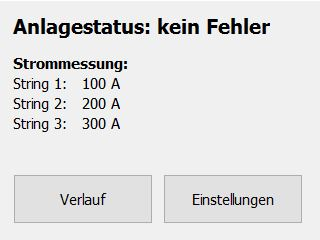
\includegraphics[width=0.475\textwidth]{images/userguide/screen0.jpg}
    \caption{Hauptmenu}
    \label{fig:software:gui:screen0}
\end{wrapfigure}

Die Benutzeroberfl\"ache  ist bewusst sehr schlicht  gehalten. Sie besteht aus
folgenden Ansichten: Hauptmen\"u, Einstellungen, Eingabe der Telefonnummer und
dem Fehlerverlauf,  gezeigt in den  Abbildungej \ref{fig:software:gui:screen0}
bis     \ref{fig:software:gui:screen4}. Die     Beschreibung    der     vollen
Funktionalit\"at  ist  im  Kapitel \emph{\titleref{chap:userguide}}  ab  Seite
\pageref{chap:userguide} zu finden.

\vspace*{6em}
\noindent\adjustbox{valign=t}{\begin{minipage}{0.475\textwidth}
    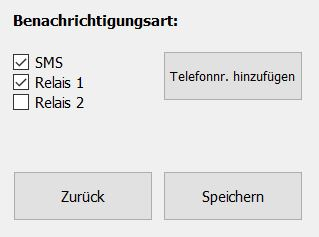
\includegraphics[width=\textwidth]{images/userguide/screen1.jpg}
    \figcaption[Master: Menu: Einstellungen]{Einstellungen}
    \label{fig:software:gui:screen1}
\end{minipage}}
\hspace*{0.04\textwidth}
\noindent\adjustbox{valign=t}{\begin{minipage}{0.475\textwidth}
    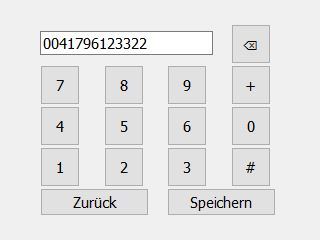
\includegraphics[width=\textwidth]{images/userguide/screen2.jpg}
    \figcaption[Master: Menu: Einstellungen: Telefonnummer]{Eingabe einer Telefonnummer}
    \label{fig:software:gui:screen2}
\end{minipage}}

\noindent\adjustbox{valign=t}{\begin{minipage}{0.475\textwidth}
    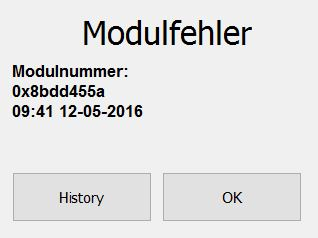
\includegraphics[width=\textwidth]{images/userguide/screen3.png}
    \figcaption[Master: Menu: Modulfehler]{Fehler bei einem Modul}
    \label{fig:software:gui:screen3}
\end{minipage}}
\hspace*{0.04\textwidth}
\noindent\adjustbox{valign=t}{\begin{minipage}{0.475\textwidth}
    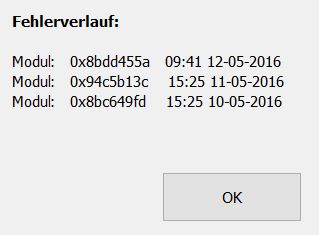
\includegraphics[width=\textwidth]{images/userguide/screen4.jpg}
    \figcaption[Master: Menu: Einstellungen: Fehlerverlauf]{Fehlerverlauf der Anlage}
    \label{fig:software:gui:screen4}
\end{minipage}}

% ---------------------------------------------------------------------------- %
\clearpage
\subsection{Datenbank}
\label{subsec:software:master:database}
% ---------------------------------------------------------------------------- %


Um  die  gesammelten  Daten  optimal  zu speichern  und  zu  einem  sp\"ateren
Zeitpunkt wieder  verwenden zu  k\"onnen, wird eine  Datenbank verwendet. Dies
hat gegen\"uber  der Verwendung von internen  Datenstrukturen wie Dictionaries
und Arrays  zwar die Nachteile von  gr\"osserem (Erst-)Implementationsaufwand,
h\"oherem  Arbeitsspeicherbedarf  und   gr\"osserem  Rechenaufwand  f\"ur  die
CPU. Jedoch   wird  die   Wartung  der   Software  und   das  Erg\"anzen   von
zus\"atzlicher   Funktionalit\"at   stark   vereinfacht. Ebenfalls   ist   die
Auswertung einfacher und  flexibler, da schon beim Auslesen der  Werte aus der
Datenbank nach verschiedenen Kriterien gefiltert werden kann.

\begin{figure}[h!tb]
    \centering
    \begin{tikzpicture}
    \sffamily
    \small
    %\graph [left anchor=east,grow right sep,right anchor=west,grow right,branch down,nodes={rounded rectangle,draw}]
    \begin{scope}[
            every node/.style = {
                draw = solarized-base02,
                rounded rectangle,
                fill=solarized-base2,
                text=solarized-base02,
                inner sep=1mm,
                text height=0.7em,
            },
            node distance=3mm,
            table/.style={
                fill=solarized-cyan,
                text=solarized-base2,
                inner sep=2mm,
            },
            column/.style={
                minimum width=25mm,
            }
        ]
        \node (database)[
            fill=solarized-blue,
            text=solarized-base2,
            inner sep=2mm
        ] at (0,0) {Datenbank};

        \node (strings)   [table,below left=15mm of database] {strings};
        \node (sID)       [column,below right=12mm of strings] {ID};
        \node (sStringNo) [column,below=of sID]            {stringnumber};
        \node (sCurr)     [column,below=of sStringNo]      {stringcurrent};
        \node (sTs)       [column,below=of sCurr]          {timestamp};
        \node (sDev)      [column,below=of sTs]            {deviation};
        \node (sReported) [column,below=of sDev]           {flag\_reported};

        \node (panels)    [table,left=of strings]  {panels};
        \node (pID)       [column,below left=12mm of panels]    {ID};
        \node (pSerial)   [column,below=of pID]       {serialnumber};
        \node (pVoltage)  [column,below=of pSerial]   {voltage};
        \node (pStringNo) [column,below=of pVoltage]  {stringnumber};
        \node (pTs)       [column,below=of pStringNo] {timestamp};
        \node (pDev)      [column,below=of pTs]       {deviation};
        \node (pReported) [column,below=of pDev]      {flag\_reported};

        \node (string1)  [table,below right=15mm of database] {string\{1,2,3\}};
        \node (s1ID)     [column,below right=12mm of string1]        {ID};
        \node (s1Serial) [column,below=of s1ID]           {serialnumber};
    \end{scope}
    \begin{scope}[on background layer]
    \end{scope}

    \begin{scope}[
            rounded corners,
            draw=solarized-base02
        ] % connections
        \draw[-latex] (database) -| (panels);
        \draw[-latex] (database) -| (strings);
        \draw[-latex] (database) -| (string1);

        \draw[-latex] (panels) |- (pID);
        \draw[-latex] (panels) |- (pSerial);
        \draw[-latex] (panels) |-  (pVoltage);
        \draw[-latex] (panels) |-  (pStringNo);
        \draw[-latex] (panels) |-  (pTs);
        \draw[-latex] (panels) |-  (pDev);
        \draw[-latex] (panels) |-  (pReported);

        \draw[-latex] (strings) |- (sID);
        \draw[-latex] (strings) |- (sStringNo);
        \draw[-latex] (strings) |- (sCurr);
        \draw[-latex] (strings) |- (sTs);
        \draw[-latex] (strings) |- (sDev);
        \draw[-latex] (strings) |- (sReported);

        \draw[-latex] (string1) |- (s1ID);
        \draw[-latex] (string1) |- (s1Serial);
    \end{scope}
\end{tikzpicture}

    \caption{Datenbank-Layout}
  \label{fig:database:layout}
\end{figure}


%stringX-tables:
Unsere Datenbank  umfasst 5 Tabellen  (oder \emph{Tables} im  Fachjargon), wie
auch in Abbildung \ref{fig:database:layout} gezeigt:

\begin{itemize}
    \tightlist
    \item
        \code{panels:} Speichert die Spannungen der PV-Module
    \item
        \code{strings:} Speichert die Str\"ome in den Strings
    \item
        \code{string1:} Speichert Sensor-IDs in String 1
    \item
        \code{string2:} Speichert Sensor-IDs in String 2
    \item
        \code{string3:} Speichert Sensor-IDs in String 3
\end{itemize}

Letztere drei  (in Abbildung \ref{fig:database:layout} auf  der rechten Seite)
davon  dienen  ausschliesslich  der  Zuordnung  aller  im  System  vorhandenen
Seriennummern  zu  den  einzelnen  Strings. Dies ist  notwendig,  um  bei  der
Auswertung  zu wissen,  welche Sensoren  sich  im selben  String befinden  und
dementsprechend miteinander verglichen  werden m\"ussen. Diese Tables bestehen
lediglich aus 2  Spalten, eine f\"ur die Seriennummer sowie  eine f\"ur die ID
des  Eintrages, welcher  ben\"otigt wird,  um doppelt  eingetragene Zeilen  zu
verhindern.

%strings-table:
Das Table \code{strings} (Mitte  in Abbildung \ref{fig:database:layout}) dient
der Speicherung  der gemessenen String-Str\"ome. Diese Werte  werden als Paket
mit einigen  wichtigen zus\"atzlichen Daten gespeichert. Dazu  geh\"oren neben
dem gemessenen Stromwert noch die  String-Nummer, um zu wissen, welcher String
gemessen worden ist,  ein Zeitstempel, um nachvollziehen zu  k\"onnen, wie alt
die Eintr\"age  sind, ein leeres  Feld, um  bei der Auswertung  die Abweichung
zum  Durchschnitt eintragen  zu k\"onnen,  sowie  ein Feld,  welches ein  Flag
beinhaltet, das  anzeigt, ob  der String bereits  als ausserhalb  der Toleranz
gemeldet  worden  ist. Zudem wird  auch  hier  wieder  eine Spalte  f\"ur  die
Eintrags-ID ben\"otigt.

%panels-table:
Das  letzte  und  gr\"osste  Table   ist  \code{panels}  (links  in  Abbildung
\ref{fig:database:layout}),  in  welchem   die  Modulspannungen  abgespeichert
werden. Auch  hier   wird  dies   wieder  als   Paket  mit   relevanten  Daten
realisiert. Die  Zeile in  diesem Table  ist grunds\"atzlich  gleich aufgebaut
wie  jene des  Strings-Table, nur  dass  hier anstelle  des String-Stroms  die
Modulspannung eingetragen sowie ein zus\"atzliches Feld f\"ur die Seriennummer
des  gemessenen  Modul-Sensors  verwendet wird. Dies  wird  hier  zus\"atzlich
ben\"otigt,  um  die  gemessenen  Daten   in  direktem  Zusammenhang  mit  den
Seriennummern  der Sensoren  zu bringen,  was f\"ur  die Auswertung  der Daten
n\"otig ist.


% ---------------------------------------------------------------------------- %
\subsection{Implementation}
\label{subsec:software:master:implementation}
% ---------------------------------------------------------------------------- %

Die  Master-Software  besteht aus  Python-Files,  auf  welche die  anfallenden
Aufgaben  verteilt  werden. Im  Folgenden  werden vier  dieser  Files  genauer
beschrieben.


% ---------------------------------------------------------------------------- %
\subsubsection{\code{database.py}}
\label{subsubsec:software:master:implementation:database}
% ---------------------------------------------------------------------------- %

Dieses File ist  dazu da, die Datenbank zu erzeugen  und zu verwalten. Mittels
SQLAlchemy wird  zuerst das Datenbank-File  erstellt und die  einzelnen Tables
gem\"ass  unseren Vorlagen  aufgebaut  und hinzugef\"ugt. Dabei  wird vor  dem
Erzeugen der einzelnen  Tabellen zuerst \"uberpr\"uft, ob  eine solche bereits
vorhanden ist. Das  stellt sicher, dass  auch bei einem Neustart  des \Master~
die  vorhandene Datenbank  nicht \"uberschrieben  wird. Nachdem die  Datenbank
erstellt  worden ist,  wird zudem  f\"ur jedes  Table eine  eigene Klasse  mit
zugeh\"origem  Mapper definiert. Diese  werden ben\"otigt,  damit gleichzeitig
ausgel\"oste Datenbank-Operationen sich  nicht gegenseitig blockieren, sondern
nacheinander abgearbeitet werden k\"onnen.


{\begin{a3pages}
\setlength{\parindentbak}{\parindent}
    \noindent\adjustbox{valign=t}{\begin{minipage}{135mm}
% ---------------------------------------------------------------------------- %
\subsubsection{\code{input\_handler.py}}
\label{subsubsec:software:master:implementation:inputHandler}
% ---------------------------------------------------------------------------- %


    Dieses File hat den Zweck,  s\"amtliche Messwerte abzufragen, einen ersten
    Teil  der Auswertung  zu  \"ubernehmen und  schlussendlich die  Eintr\"age
    in  der  Datenbank  vorzunehmen. F\"ur  die  Abfrage  der  Messdaten  wird
    hier  die gesamte  Kommunikation  \"uber \ISC~  implementiert.  Da  dieses
    File  sehr umfangreich  ist,  ist der  zugeh\"orige  Prozess in  Abbildung
    \ref{fig:inputHandler} grafisch dargestellt.

    \setlength{\parindent}{\parindentbak} % restore  paragraph indentation Der
    Hauptablauf startet mit  der Methode \code{stringcurrents\_request}. Diese
    ruft nacheinander mittels der Methode \code{read\_stringcurrents\_i2c} die
    aktuellen  Werte der  Stringstr\"ome ab  und speichert  diese auch  gleich
    mittels  \code{write\_string\_into\_database}  am  richtigen  Ort  in  der
    Datenbank. Anschliessend  sollen die  soeben ausgelesenen  Stromwerte auch
    gleich ausgewertet werden. Da dies  keinen grossen Aufwand darstellt, wird
    dies ebenfalls  im selben File implementiert. Daf\"ur  wird im Hauptablauf
    als  n\"achstes  die  Methode  \code{string\_compare}  ausgef\"uhrt. Diese
    berechnet den Durchschnitt der aktuellen  Werte sowie die Abweichungen der
    einzelnen  Strings  zu  diesem. Ist  die Abweichung  zu  gross,  wird  der
    String dem  Benutzer gemeldet. Dies dient  vor allem dazu,  grobe Probleme
    festzustellen und  diese z\"ugig melden zu  k\"onnen. Ausf\"alle einzelner
    Module dagegen werden vom File \code{evaluator.py} detektiert.

    Nach  den   Str\"omen  widmet   sich  das  File   den  Modulspannungen. Im
    Hauptablauf  des  Files  wird  die  Methode  \code{modulevoltage\_request}
    aufgerufen,  welche   in  jedem   String  die   vorhandenen  Seriennummern
    durchgeht  und dabei  f\"ur  jede mittels  \code{read\_modulevoltage\_i2c}
    einen   Request  aussendet. Wird   keine  Antwort   empfangen,  wird   die
    History   dieser  Seriennummer   \"uberpr\"uft   –   ist  w\"ahrend   24
    Stunden  kein   Eintrag  gemacht  worden,   wird  das  Modul   als  defekt
    gemeldet. Bekommt  die Software  eine Antwort  auf den  Request, wird  der
    Wert  unter  Verwendung  der  Methode  \code{write\_panel\_into\_database}
    in   die  Datenbank   geschrieben. Zus\"atzlich  wird   \"uberpr\"uft,  ob
    die   Seriennummer   bereits   im  zugeh\"origen   Stringpanel   vorhanden
    ist. So  wird   ein  neu   eingesetztes  Solarmodul   automatisch  erkannt
    und   per   \code{write\_stringX\_into\_database}  dem   richtigen   Table
    hinzugef\"ugt. Nachdem  alle  Spannungen  abgefragt sind  wird  auch  hier
    bereits die Grundlage f\"ur die Auswertung gelegt. So wird in jedem String
    der h\"ochste Eintrag der Messreihe  gesucht und bei jedem einzelnen Modul
    im  \code{deviation}-Feld  die  Abweichung  zu  diesem  eingetragen. Somit
    wird immer  der aktuelle  Wert mit  dem einer  funktionierenden Solarzelle
    verglichen. Bei einer  funktionierenden Zelle  treten somit  lediglich bei
    Abschattungen  kurzzeitig  grosse  Differenzen  auf,  welche  aber  \"uber
    den  Tag  gemittelt  keinen  sehr  grossen  Einfluss  haben. So  kann  gut
    zwischen tempor\"ar abgeschatteten  Modulen, welche eigentlich einwandfrei
    funktionieren,   und   defekten   Modulen,  die   l\"angerfristig   grosse
    Abweichungen aufzeigen, unterschieden werden.

    \vspace*{5mm}

    \hfill\adjustbox{valign=t}{\begin{minipage}{52mm}
        \figcaption
        [Ablaufdiagramm \code{input\_handler.py}]
        {Ablaufdiagramm \protect\\\code{input\_handler.py}}
        \label{fig:inputHandler}
    \end{minipage}}
\end{minipage}}
\hspace*{25mm}
\adjustbox{valign=t}{\begin{minipage}{195mm}
    \begin{tikzpicture}[%
        align=center,
        text=solarized-base02,
        draw=solarized-base02,
        remember picture,
        overlay,
    ]
    \small
    \ttfamily

    \begin{scope}[
        every node/.style = draw,
        terminal/.append style={
            rounded rectangle,
            fill=solarized-violet,
            text=solarized-base3,
            inner sep=2mm,
        }, % data packages
        sign/.style={
            inner sep=2mm,
            rounded corners=1mm,
            fill=solarized-magenta,
            text=solarized-base3,
        },         % custom signal style
        circ/.style={
            inner sep=2mm,
            rounded corners=1mm,
            double,
            fill=solarized-base02,
            draw=solarized-base02,
            text=solarized-base2,
        }, % circuitry
        proc/.style={
            inner sep=2mm,
            rounded corners=1mm,
            fill=solarized-cyan,
            text=solarized-base3,
        },       % process/activity
        stor/.style={
            fill=cyan!30
        },         % storage
        dbtable/.style={
            text=solarized-base3,
            draw=solarized-base3,
            rounded corners=1mm,
            inner sep=2mm,
        } % database tables
    ]
        %\node (stringcurrents-request) [
        %    sign,
        %    signal,
        %    signal to=east
        %] at (10mm,0mm) {stringcurrents\_request};

        \node (stringcurrents-request) [
            proc,
        ] at (20mm,-20mm) {stringcurrents\_request};

        %\node (string-support) [
        %    right=30mm of stringcurrents-request,
        %    draw=white,
        %] { };

        \node (stringnumber) [
            sign,
            signal,
            signal to=east,
            signal from=west,
            above right=20mm of stringcurrents-request,
        ] {stringnumber};

        \node (stringcurrentget) [
            sign,
            signal,
            signal to=west,
            signal from=east,
            right=20mm of stringcurrents-request,
        ] {stringcurrent};

        \node (read-stringcurrents-i2c) [
            proc,
            right=of stringcurrentget,
        ] {read\_stringcurrents\_i2c};

        \node (write-string-into-database) [
            proc,
            below=of read-stringcurrents-i2c,
        ] {write\_string\_into\_database};

        \node (stringcurrentput) [
            sign,
            signal,
            signal to=east,
            signal from=west,
            left=of write-string-into-database,
        ] {stringcurrent};

        %\node (string-compare) [
        %    terminal,
        %    below=20mm of stringcurrents-request,
        %] {string\_compare};

        \node (string-compare) [
            proc,
            below=20mm of stringcurrents-request,
        ] {string\_compare};

        \node (modulevoltage-request) [
            proc,
            below=20mm of string-compare,
        ] {modulevoltage\_request};

        \node (stringNo-serialNo) [
            sign,
            signal,
            signal to=east,
            signal from=west,
            right=20mm of modulevoltage-request,
            align=center,
        ] {stringnumber\\serialnumber};

        \node (serialNo-voltage) [
            sign,
            signal,
            signal to=west,
            signal from=east,
            below=of stringNo-serialNo,
            align=center,
        ] {serialnumber\\voltage};

        \node (read-modulevoltage-i2c) [
            proc,
            right=of stringNo-serialNo,
        ] {read\_modulevoltage\_i2c};

        \node (serialNo-stringNo-voltage) [
            sign,
            signal,
            signal to=south,
            signal from=north,
            below=60mm of modulevoltage-request,
            align=center,
        ] {serialnumber\\stringnumber\\voltage};

        \node (support1) [
            fill=white,
            draw=white,
            above=of serialNo-stringNo-voltage,
        ] { };

        \node (write-panel-into-database) [
            proc,
            below=of serialNo-stringNo-voltage,
        ] {write\_panel\_into\_database};

        \node (serialNo1) [
            sign,
            signal,
            signal to=east,
            signal from=west,
            right=of write-panel-into-database,
        ] {serialnumber};

        \node (write-string1-into-database) [
            proc,
            above right=of serialNo1,
        ] {write\_string1\_into\_database};

        \node (write-string2-into-database) [
            proc,
            below=of write-string1-into-database,
        ] {write\_string2\_into\_database};

        \node (write-string3-into-database) [
            proc,
            below=of write-string2-into-database,
        ] {write\_string3\_into\_database};
    \end{scope}

    \begin{scope}[on background layer]
        \node (getStringCurrents) [%
            draw,
            double,
            rounded corners=5mm,
            fill=solarized-base3,
            inner sep=1.75em,
            fit=(read-stringcurrents-i2c) (write-string-into-database) (stringnumber) (stringcurrentget) (stringcurrentput),
            text height=-0.5em,
            align=right,
        ] {\sffamily wird pro String $1\times$ ausgef\"uhrt, also total $3\times$};

        \node (getModuleVoltages) [%
            draw,
            double,
            rounded corners=5mm,
            fill=solarized-base3,
            inner sep=1.75em,
            fit=(read-modulevoltage-i2c) (stringNo-serialNo) (serialNo-voltage),
            text height=-0.5em,
            align=right,
        ] {\sffamily mit Schlaufe f\"ur jedes Modul ausgef\"uhrt};

        \node (checkSN) [%
            draw,
            double,
            rounded corners=5mm,
            fill=solarized-base3,
            inner sep=1.75em,
            fit=(serialNo-stringNo-voltage) (write-panel-into-database) (serialNo1) (write-string1-into-database) (write-string2-into-database) (write-string3-into-database) (support1),
            text height=-0.5em,
            align=right,
        ] {\sffamily SN wird \"uberpr\"uft und in das entsprechende Table\\eingetragen, falls noch kein Eintrag vorhanden ist.};

        \node (mainProcess) [%
            draw,
            double,
            rounded corners=5mm,
            fill=solarized-base2,
            inner sep=1.5em,
            fit=(stringcurrents-request) (string-compare) (modulevoltage-request),
            text height=-0.5em,
            align=right,
            text=solarized-base02,
        ] {\sffamily Hauptablauf des Files};
    \end{scope}


    \begin{scope}[
            rounded corners,
            every path/.append style={draw=solarized-base03,},
    ]
        \draw[-latex] (stringcurrents-request) |- (stringnumber);
        \draw[-latex] (stringnumber) -| (read-stringcurrents-i2c);
        \draw[-latex] (read-stringcurrents-i2c) -- (stringcurrentget);
        \draw[-latex] (stringcurrentget) -- (stringcurrents-request);
        \draw[-latex] (stringcurrents-request) |- (stringcurrentput);
        \draw[-latex] (stringcurrentput) -- (write-string-into-database);

        \draw[-latex] (stringcurrents-request) -- (string-compare);
        \draw[-latex] (string-compare) -- (modulevoltage-request);

        \draw[-latex] (modulevoltage-request) -- (stringNo-serialNo);
        \draw[-latex] (stringNo-serialNo) -- (read-modulevoltage-i2c);
        \draw[-latex] (read-modulevoltage-i2c) |- (serialNo-voltage);
        \draw[-latex] (serialNo-voltage) -| (modulevoltage-request);


        \draw[-latex] (modulevoltage-request) -- (serialNo-stringNo-voltage);
        \draw[-latex] (serialNo-stringNo-voltage) -- (write-panel-into-database);
        \draw[-latex] (write-panel-into-database) -- (serialNo1);
        \draw[dashed,-latex] (serialNo1) |- (write-string1-into-database);
        \draw[dashed,-latex] (serialNo1) -- (write-string2-into-database);
        \draw[dashed,-latex] (serialNo1) |- (write-string3-into-database);
    \end{scope}

\end{tikzpicture}

\end{minipage}}

\end{a3pages}}



% ---------------------------------------------------------------------------- %
\subsubsection{\code{evaluator.py}}
\label{subsubsec:software:master:implementation:evaluator}
% ---------------------------------------------------------------------------- %

Der  Evaluator ist  f\"ur die  Auswertung der  Modulspannungen zust\"andig. Er
wird  einmal  t\"aglich ausgef\"uhrt  und  kontrolliert  die Spannungen  aller
Module des Systems innerhalb der letzten 24 Stunden.

Daf\"ur  wird zuerst  f\"ur  jeden String  eine Liste  mit  den aktuell  darin
vorhandenen  Seriennummern  erstellt. Innerhalb  jedes Strings  wird  wiederum
f\"ur  jedes Modul  eine Liste  mit den  Abweichungen jeder  einzelnen Messung
w\"ahrend der  letzten 24 Stunden  erstellt. Nun wird \"uber die  gesamte Zeit
der quadratische Mittelwert der  Abweichungen gebildet. Aus allen Mittelwerten
der   Module  innerhalb   eines  Strings   wird  nun   die  Standardabweichung
berechnet. Liegt ein  Modul ausserhalb dieser  Abweichung, wird es  als defekt
gemeldet. Dieses Vorgehen  ist zwar relativ kompliziert,  garantiert aber dass
nur Module  gemeldet werden, welche  \"uber l\"angere Dauer zu  wenig Leistung
bringen. Dies  erh\"oht  die  Zuverl\"assigkeit   des  Systems  und  reduziert
die  Wahrscheinlichkeit, eines  Fehlalarms,  welcher  dem Benutzer  unn\"otige
Umst\"ande bereiten w\"urde.


% ---------------------------------------------------------------------------- %
\subsubsection{\code{reporter.py}}
\label{subsubsec:software:master:implementation:reporter}
% ---------------------------------------------------------------------------- %

Der  Reporter hat  die Aufgabe,  bei  einem detektierten  Fehler den  Benutzer
\"uber  diesen zu  informieren. Dies  geschieht, indem  er einerseits  daf\"ur
sorgt,  dass   im  GUI  das  Fehlermeldungs-Display   mit  der  entsprechenden
Seriennummer  angezeigt wird. Zudem  werden  die Relaiskontakte  angesprochen,
um  einen beliebigen  externen  Alarm auszul\"osen. Letztlich  wird auch  noch
das  GSM-Modul  aktiviert,  um  auf die  hinterlegte  Mobiltelefonnummer  eine
Textnachricht zu senden.

% **************************************************************************** %
\chapter{Validierung}
\label{chap:validierung}
% **************************************************************************** %

Im Folgenden werden  Messungen unserer Kopplungsspule, des  Modulators und des
Demodulators sowie eine Evaluation unseres Gesamtsystems pr\"asentiert.

% ---------------------------------------------------------------------------- %
\section{Kopplungsspule}
\label{sec:val:coupling:coil}
% ---------------------------------------------------------------------------- %

Eine  Spule  leitet nicht  alle  Frequenzen  gleich gut. Zudem  s\"attigt  ein
Ferritkern  ab einem  bestimmten  Strom. Deswegen  werden Frequenzg\"ange  der
Spule mit dem Ferritkern und  ein Power-Choke Test mit einer Sekund\"arwindung
gemacht.

Es   wird   die   Induktivit\"at   einer  Spule   getestet,   welche   mehrere
Windungen  \"ubereinander  hat  und  einer  Spule,  welche  nur  eine  Schicht
mit  Wicklungen   hat. Beide  Spulen   haben  genau  30   Wicklungen. Wie  man
Abbildung~\ref{fig:meas:coupling:coil:L}  entnehmen kann,  ist  die Spule  mit
nur  einer Wicklungsschicht  bis  \"uber 20  Megahertz  induktiv (blaue  Kurve
in Abbildung  \ref{fig:meas:coupling:coil:L}), w\"ahrend  die Multilayer-Spule
schon   bei   4   Megahertz   kapazitiv  wird   (rote   Kurve   in   Abbildung
\ref{fig:meas:coupling:coil:L}). F\"ur  unser   Projekt  haben   wir  deswegen
die  einschichtige  Spule   gew\"ahlt. Eine  Messung  der  Streuinduktivit\"at
der   gew\"ahlten  Spule   ist  ebenfalls   gemacht  worden,   um  gut   damit
rechnen   und   simulieren   zu   k\"onnen   (gr\"une   Kurve   in   Abbildung
\ref{fig:meas:coupling:coil:L}).

\clearpage
\begin{figure}[h!tb]
    \centering
    %% Creator: Matplotlib, PGF backend
%%
%% To include the figure in your LaTeX document, write
%%   \input{<filename>.pgf}
%%
%% Make sure the required packages are loaded in your preamble
%%   \usepackage{pgf}
%%
%% Figures using additional raster images can only be included by \input if
%% they are in the same directory as the main LaTeX file. For loading figures
%% from other directories you can use the `import` package
%%   \usepackage{import}
%% and then include the figures with
%%   \import{<path to file>}{<filename>.pgf}
%%
%% Matplotlib used the following preamble
%%   \usepackage{fontspec}
%%   \setmainfont{Bitstream Vera Serif}
%%   \setsansfont{Bitstream Vera Sans}
%%   \setmonofont{Bitstream Vera Sans Mono}
%%
\begingroup%
\makeatletter%
\begin{pgfpicture}%
\pgfpathrectangle{\pgfpointorigin}{\pgfqpoint{5.500000in}{2.000000in}}%
\pgfusepath{use as bounding box, clip}%
\begin{pgfscope}%
\pgfsetbuttcap%
\pgfsetmiterjoin%
\pgfsetlinewidth{0.000000pt}%
\definecolor{currentstroke}{rgb}{0.000000,0.000000,0.000000}%
\pgfsetstrokecolor{currentstroke}%
\pgfsetstrokeopacity{0.000000}%
\pgfsetdash{}{0pt}%
\pgfpathmoveto{\pgfqpoint{0.000000in}{0.000000in}}%
\pgfpathlineto{\pgfqpoint{5.500000in}{0.000000in}}%
\pgfpathlineto{\pgfqpoint{5.500000in}{2.000000in}}%
\pgfpathlineto{\pgfqpoint{0.000000in}{2.000000in}}%
\pgfpathclose%
\pgfusepath{}%
\end{pgfscope}%
\begin{pgfscope}%
\pgfsetbuttcap%
\pgfsetmiterjoin%
\pgfsetlinewidth{0.000000pt}%
\definecolor{currentstroke}{rgb}{0.000000,0.000000,0.000000}%
\pgfsetstrokecolor{currentstroke}%
\pgfsetstrokeopacity{0.000000}%
\pgfsetdash{}{0pt}%
\pgfpathmoveto{\pgfqpoint{0.550000in}{0.400000in}}%
\pgfpathlineto{\pgfqpoint{5.225000in}{0.400000in}}%
\pgfpathlineto{\pgfqpoint{5.225000in}{1.800000in}}%
\pgfpathlineto{\pgfqpoint{0.550000in}{1.800000in}}%
\pgfpathclose%
\pgfusepath{}%
\end{pgfscope}%
\begin{pgfscope}%
\pgfpathrectangle{\pgfqpoint{0.550000in}{0.400000in}}{\pgfqpoint{4.675000in}{1.400000in}} %
\pgfusepath{clip}%
\pgfsetrectcap%
\pgfsetroundjoin%
\pgfsetlinewidth{0.501875pt}%
\definecolor{currentstroke}{rgb}{0.000000,0.000000,1.000000}%
\pgfsetstrokecolor{currentstroke}%
\pgfsetdash{}{0pt}%
\pgfpathmoveto{\pgfqpoint{0.550000in}{1.474480in}}%
\pgfpathlineto{\pgfqpoint{0.644468in}{1.473704in}}%
\pgfpathlineto{\pgfqpoint{0.691701in}{1.474025in}}%
\pgfpathlineto{\pgfqpoint{0.738935in}{1.473568in}}%
\pgfpathlineto{\pgfqpoint{0.857020in}{1.472725in}}%
\pgfpathlineto{\pgfqpoint{0.998721in}{1.471731in}}%
\pgfpathlineto{\pgfqpoint{1.140422in}{1.470260in}}%
\pgfpathlineto{\pgfqpoint{1.305740in}{1.468630in}}%
\pgfpathlineto{\pgfqpoint{1.518292in}{1.465763in}}%
\pgfpathlineto{\pgfqpoint{1.612760in}{1.463738in}}%
\pgfpathlineto{\pgfqpoint{1.848929in}{1.459121in}}%
\pgfpathlineto{\pgfqpoint{2.203182in}{1.450546in}}%
\pgfpathlineto{\pgfqpoint{2.486585in}{1.443334in}}%
\pgfpathlineto{\pgfqpoint{2.817221in}{1.435884in}}%
\pgfpathlineto{\pgfqpoint{3.147858in}{1.431032in}}%
\pgfpathlineto{\pgfqpoint{3.360410in}{1.430087in}}%
\pgfpathlineto{\pgfqpoint{3.549345in}{1.432512in}}%
\pgfpathlineto{\pgfqpoint{3.714663in}{1.438605in}}%
\pgfpathlineto{\pgfqpoint{3.856364in}{1.449201in}}%
\pgfpathlineto{\pgfqpoint{3.927215in}{1.456958in}}%
\pgfpathlineto{\pgfqpoint{3.998066in}{1.467652in}}%
\pgfpathlineto{\pgfqpoint{4.045299in}{1.476776in}}%
\pgfpathlineto{\pgfqpoint{4.092533in}{1.488420in}}%
\pgfpathlineto{\pgfqpoint{4.139767in}{1.503276in}}%
\pgfpathlineto{\pgfqpoint{4.163384in}{1.511970in}}%
\pgfpathlineto{\pgfqpoint{4.210618in}{1.533551in}}%
\pgfpathlineto{\pgfqpoint{4.234235in}{1.546815in}}%
\pgfpathlineto{\pgfqpoint{4.257851in}{1.562193in}}%
\pgfpathlineto{\pgfqpoint{4.281468in}{1.556961in}}%
\pgfpathlineto{\pgfqpoint{4.305085in}{1.572718in}}%
\pgfpathlineto{\pgfqpoint{4.328702in}{1.590345in}}%
\pgfpathlineto{\pgfqpoint{4.375936in}{1.633204in}}%
\pgfpathlineto{\pgfqpoint{4.446787in}{1.710316in}}%
\pgfpathlineto{\pgfqpoint{4.470403in}{1.724386in}}%
\pgfpathlineto{\pgfqpoint{4.494020in}{1.697391in}}%
\pgfpathlineto{\pgfqpoint{4.517637in}{1.658899in}}%
\pgfpathlineto{\pgfqpoint{4.541254in}{1.492111in}}%
\pgfpathlineto{\pgfqpoint{4.564871in}{1.192092in}}%
\pgfpathlineto{\pgfqpoint{4.588488in}{0.907691in}}%
\pgfpathlineto{\pgfqpoint{4.612105in}{0.692464in}}%
\pgfpathlineto{\pgfqpoint{4.635722in}{0.624894in}}%
\pgfpathlineto{\pgfqpoint{4.659339in}{0.618937in}}%
\pgfpathlineto{\pgfqpoint{4.682955in}{0.650846in}}%
\pgfpathlineto{\pgfqpoint{4.706572in}{0.708890in}}%
\pgfpathlineto{\pgfqpoint{4.777423in}{0.822108in}}%
\pgfpathlineto{\pgfqpoint{4.801040in}{0.851263in}}%
\pgfpathlineto{\pgfqpoint{4.824657in}{0.872842in}}%
\pgfpathlineto{\pgfqpoint{4.848274in}{0.889344in}}%
\pgfpathlineto{\pgfqpoint{4.871891in}{0.902940in}}%
\pgfpathlineto{\pgfqpoint{4.895507in}{0.907433in}}%
\pgfpathlineto{\pgfqpoint{4.919124in}{0.905990in}}%
\pgfpathlineto{\pgfqpoint{4.942741in}{0.888958in}}%
\pgfpathlineto{\pgfqpoint{4.966358in}{0.836468in}}%
\pgfpathlineto{\pgfqpoint{4.989975in}{0.881629in}}%
\pgfpathlineto{\pgfqpoint{5.013592in}{1.191663in}}%
\pgfpathlineto{\pgfqpoint{5.037209in}{1.141574in}}%
\pgfpathlineto{\pgfqpoint{5.060826in}{1.114671in}}%
\pgfpathlineto{\pgfqpoint{5.084443in}{1.102061in}}%
\pgfpathlineto{\pgfqpoint{5.108059in}{1.095902in}}%
\pgfpathlineto{\pgfqpoint{5.131676in}{1.092952in}}%
\pgfpathlineto{\pgfqpoint{5.178910in}{1.091502in}}%
\pgfpathlineto{\pgfqpoint{5.235000in}{1.092926in}}%
\pgfpathlineto{\pgfqpoint{5.235000in}{1.092926in}}%
\pgfusepath{stroke}%
\end{pgfscope}%
\begin{pgfscope}%
\pgfpathrectangle{\pgfqpoint{0.550000in}{0.400000in}}{\pgfqpoint{4.675000in}{1.400000in}} %
\pgfusepath{clip}%
\pgfsetrectcap%
\pgfsetroundjoin%
\pgfsetlinewidth{0.501875pt}%
\definecolor{currentstroke}{rgb}{0.000000,0.500000,0.000000}%
\pgfsetstrokecolor{currentstroke}%
\pgfsetdash{}{0pt}%
\pgfpathmoveto{\pgfqpoint{0.550000in}{1.467111in}}%
\pgfpathlineto{\pgfqpoint{0.762552in}{1.457307in}}%
\pgfpathlineto{\pgfqpoint{0.857020in}{1.450749in}}%
\pgfpathlineto{\pgfqpoint{0.951487in}{1.441846in}}%
\pgfpathlineto{\pgfqpoint{1.045955in}{1.430833in}}%
\pgfpathlineto{\pgfqpoint{1.140422in}{1.416546in}}%
\pgfpathlineto{\pgfqpoint{1.282124in}{1.390023in}}%
\pgfpathlineto{\pgfqpoint{1.447442in}{1.353982in}}%
\pgfpathlineto{\pgfqpoint{1.565526in}{1.327961in}}%
\pgfpathlineto{\pgfqpoint{1.683611in}{1.304579in}}%
\pgfpathlineto{\pgfqpoint{1.778078in}{1.288782in}}%
\pgfpathlineto{\pgfqpoint{1.896163in}{1.273207in}}%
\pgfpathlineto{\pgfqpoint{1.990630in}{1.263826in}}%
\pgfpathlineto{\pgfqpoint{2.108715in}{1.255212in}}%
\pgfpathlineto{\pgfqpoint{2.226799in}{1.249123in}}%
\pgfpathlineto{\pgfqpoint{2.321267in}{1.245535in}}%
\pgfpathlineto{\pgfqpoint{2.486585in}{1.241066in}}%
\pgfpathlineto{\pgfqpoint{2.746371in}{1.236525in}}%
\pgfpathlineto{\pgfqpoint{3.100624in}{1.231927in}}%
\pgfpathlineto{\pgfqpoint{3.313176in}{1.230003in}}%
\pgfpathlineto{\pgfqpoint{3.572962in}{1.229180in}}%
\pgfpathlineto{\pgfqpoint{3.809131in}{1.230669in}}%
\pgfpathlineto{\pgfqpoint{3.927215in}{1.232678in}}%
\pgfpathlineto{\pgfqpoint{4.068916in}{1.237305in}}%
\pgfpathlineto{\pgfqpoint{4.139767in}{1.241232in}}%
\pgfpathlineto{\pgfqpoint{4.210618in}{1.246729in}}%
\pgfpathlineto{\pgfqpoint{4.257851in}{1.251695in}}%
\pgfpathlineto{\pgfqpoint{4.281468in}{1.251465in}}%
\pgfpathlineto{\pgfqpoint{4.328702in}{1.257720in}}%
\pgfpathlineto{\pgfqpoint{4.375936in}{1.265928in}}%
\pgfpathlineto{\pgfqpoint{4.423170in}{1.276654in}}%
\pgfpathlineto{\pgfqpoint{4.446787in}{1.283354in}}%
\pgfpathlineto{\pgfqpoint{4.470403in}{1.292948in}}%
\pgfpathlineto{\pgfqpoint{4.517637in}{1.316663in}}%
\pgfpathlineto{\pgfqpoint{4.541254in}{1.331523in}}%
\pgfpathlineto{\pgfqpoint{4.564871in}{1.349600in}}%
\pgfpathlineto{\pgfqpoint{4.588488in}{1.373287in}}%
\pgfpathlineto{\pgfqpoint{4.612105in}{1.398944in}}%
\pgfpathlineto{\pgfqpoint{4.659339in}{1.469016in}}%
\pgfpathlineto{\pgfqpoint{4.682955in}{1.476561in}}%
\pgfpathlineto{\pgfqpoint{4.706572in}{1.394537in}}%
\pgfpathlineto{\pgfqpoint{4.730189in}{1.096274in}}%
\pgfpathlineto{\pgfqpoint{4.753806in}{0.825434in}}%
\pgfpathlineto{\pgfqpoint{4.777423in}{0.770782in}}%
\pgfpathlineto{\pgfqpoint{4.801040in}{0.809198in}}%
\pgfpathlineto{\pgfqpoint{4.848274in}{0.892652in}}%
\pgfpathlineto{\pgfqpoint{4.871891in}{0.921365in}}%
\pgfpathlineto{\pgfqpoint{4.895507in}{0.946526in}}%
\pgfpathlineto{\pgfqpoint{4.919124in}{0.965318in}}%
\pgfpathlineto{\pgfqpoint{4.942741in}{0.977008in}}%
\pgfpathlineto{\pgfqpoint{4.966358in}{0.983965in}}%
\pgfpathlineto{\pgfqpoint{4.989975in}{0.982188in}}%
\pgfpathlineto{\pgfqpoint{5.013592in}{0.962151in}}%
\pgfpathlineto{\pgfqpoint{5.037209in}{0.862752in}}%
\pgfpathlineto{\pgfqpoint{5.060826in}{1.182289in}}%
\pgfpathlineto{\pgfqpoint{5.084443in}{1.121718in}}%
\pgfpathlineto{\pgfqpoint{5.108059in}{1.103336in}}%
\pgfpathlineto{\pgfqpoint{5.131676in}{1.096614in}}%
\pgfpathlineto{\pgfqpoint{5.155293in}{1.094023in}}%
\pgfpathlineto{\pgfqpoint{5.202527in}{1.093316in}}%
\pgfpathlineto{\pgfqpoint{5.235000in}{1.094171in}}%
\pgfpathlineto{\pgfqpoint{5.235000in}{1.094171in}}%
\pgfusepath{stroke}%
\end{pgfscope}%
\begin{pgfscope}%
\pgfpathrectangle{\pgfqpoint{0.550000in}{0.400000in}}{\pgfqpoint{4.675000in}{1.400000in}} %
\pgfusepath{clip}%
\pgfsetrectcap%
\pgfsetroundjoin%
\pgfsetlinewidth{0.501875pt}%
\definecolor{currentstroke}{rgb}{1.000000,0.000000,0.000000}%
\pgfsetstrokecolor{currentstroke}%
\pgfsetdash{}{0pt}%
\pgfpathmoveto{\pgfqpoint{0.550000in}{1.806246in}}%
\pgfpathlineto{\pgfqpoint{0.691701in}{1.804813in}}%
\pgfpathlineto{\pgfqpoint{0.738935in}{1.805013in}}%
\pgfpathlineto{\pgfqpoint{0.904253in}{1.801622in}}%
\pgfpathlineto{\pgfqpoint{0.927870in}{1.802531in}}%
\pgfpathlineto{\pgfqpoint{0.951487in}{1.801594in}}%
\pgfpathlineto{\pgfqpoint{0.998721in}{1.801363in}}%
\pgfpathlineto{\pgfqpoint{1.187656in}{1.798032in}}%
\pgfpathlineto{\pgfqpoint{1.282124in}{1.795804in}}%
\pgfpathlineto{\pgfqpoint{1.423825in}{1.792670in}}%
\pgfpathlineto{\pgfqpoint{1.683611in}{1.785042in}}%
\pgfpathlineto{\pgfqpoint{1.896163in}{1.777928in}}%
\pgfpathlineto{\pgfqpoint{1.943396in}{1.776116in}}%
\pgfpathlineto{\pgfqpoint{2.132332in}{1.769586in}}%
\pgfpathlineto{\pgfqpoint{2.203182in}{1.766733in}}%
\pgfpathlineto{\pgfqpoint{2.415734in}{1.760543in}}%
\pgfpathlineto{\pgfqpoint{2.628286in}{1.759120in}}%
\pgfpathlineto{\pgfqpoint{2.699137in}{1.760895in}}%
\pgfpathlineto{\pgfqpoint{2.769988in}{1.763952in}}%
\pgfpathlineto{\pgfqpoint{2.840838in}{1.769013in}}%
\pgfpathlineto{\pgfqpoint{2.935306in}{1.780544in}}%
\pgfpathlineto{\pgfqpoint{2.982540in}{1.789360in}}%
\pgfpathlineto{\pgfqpoint{3.029773in}{1.800398in}}%
\pgfpathlineto{\pgfqpoint{3.061158in}{1.810000in}}%
\pgfpathmoveto{\pgfqpoint{3.612598in}{1.810000in}}%
\pgfpathlineto{\pgfqpoint{3.617529in}{0.390000in}}%
\pgfpathmoveto{\pgfqpoint{3.776482in}{0.390000in}}%
\pgfpathlineto{\pgfqpoint{3.785514in}{0.446351in}}%
\pgfpathlineto{\pgfqpoint{3.809131in}{0.556532in}}%
\pgfpathlineto{\pgfqpoint{3.832748in}{0.641583in}}%
\pgfpathlineto{\pgfqpoint{3.856364in}{0.709061in}}%
\pgfpathlineto{\pgfqpoint{3.879981in}{0.763567in}}%
\pgfpathlineto{\pgfqpoint{3.903598in}{0.808419in}}%
\pgfpathlineto{\pgfqpoint{3.927215in}{0.845835in}}%
\pgfpathlineto{\pgfqpoint{3.950832in}{0.877331in}}%
\pgfpathlineto{\pgfqpoint{3.974449in}{0.904149in}}%
\pgfpathlineto{\pgfqpoint{3.998066in}{0.927120in}}%
\pgfpathlineto{\pgfqpoint{4.021683in}{0.947008in}}%
\pgfpathlineto{\pgfqpoint{4.045299in}{0.964277in}}%
\pgfpathlineto{\pgfqpoint{4.068916in}{0.979376in}}%
\pgfpathlineto{\pgfqpoint{4.092533in}{0.992605in}}%
\pgfpathlineto{\pgfqpoint{4.116150in}{1.004270in}}%
\pgfpathlineto{\pgfqpoint{4.163384in}{1.023706in}}%
\pgfpathlineto{\pgfqpoint{4.210618in}{1.039082in}}%
\pgfpathlineto{\pgfqpoint{4.257851in}{1.051351in}}%
\pgfpathlineto{\pgfqpoint{4.328702in}{1.065259in}}%
\pgfpathlineto{\pgfqpoint{4.399553in}{1.075619in}}%
\pgfpathlineto{\pgfqpoint{4.470403in}{1.083302in}}%
\pgfpathlineto{\pgfqpoint{4.564871in}{1.090683in}}%
\pgfpathlineto{\pgfqpoint{4.682955in}{1.097007in}}%
\pgfpathlineto{\pgfqpoint{4.919124in}{1.107679in}}%
\pgfpathlineto{\pgfqpoint{4.966358in}{1.112796in}}%
\pgfpathlineto{\pgfqpoint{4.989975in}{1.117916in}}%
\pgfpathlineto{\pgfqpoint{5.013592in}{1.128773in}}%
\pgfpathlineto{\pgfqpoint{5.037209in}{1.156609in}}%
\pgfpathlineto{\pgfqpoint{5.060826in}{1.044582in}}%
\pgfpathlineto{\pgfqpoint{5.084443in}{1.073780in}}%
\pgfpathlineto{\pgfqpoint{5.108059in}{1.084196in}}%
\pgfpathlineto{\pgfqpoint{5.131676in}{1.089085in}}%
\pgfpathlineto{\pgfqpoint{5.178910in}{1.093786in}}%
\pgfpathlineto{\pgfqpoint{5.235000in}{1.096427in}}%
\pgfpathlineto{\pgfqpoint{5.235000in}{1.096427in}}%
\pgfusepath{stroke}%
\end{pgfscope}%
\begin{pgfscope}%
\pgfsetrectcap%
\pgfsetmiterjoin%
\pgfsetlinewidth{0.501875pt}%
\definecolor{currentstroke}{rgb}{0.000000,0.000000,0.000000}%
\pgfsetstrokecolor{currentstroke}%
\pgfsetdash{}{0pt}%
\pgfpathmoveto{\pgfqpoint{0.550000in}{0.400000in}}%
\pgfpathlineto{\pgfqpoint{0.550000in}{1.800000in}}%
\pgfusepath{stroke}%
\end{pgfscope}%
\begin{pgfscope}%
\pgfsetrectcap%
\pgfsetmiterjoin%
\pgfsetlinewidth{0.501875pt}%
\definecolor{currentstroke}{rgb}{0.000000,0.000000,0.000000}%
\pgfsetstrokecolor{currentstroke}%
\pgfsetdash{}{0pt}%
\pgfpathmoveto{\pgfqpoint{0.550000in}{0.400000in}}%
\pgfpathlineto{\pgfqpoint{5.225000in}{0.400000in}}%
\pgfusepath{stroke}%
\end{pgfscope}%
\begin{pgfscope}%
\pgfsetrectcap%
\pgfsetmiterjoin%
\pgfsetlinewidth{0.501875pt}%
\definecolor{currentstroke}{rgb}{0.000000,0.000000,0.000000}%
\pgfsetstrokecolor{currentstroke}%
\pgfsetdash{}{0pt}%
\pgfpathmoveto{\pgfqpoint{5.225000in}{0.400000in}}%
\pgfpathlineto{\pgfqpoint{5.225000in}{1.800000in}}%
\pgfusepath{stroke}%
\end{pgfscope}%
\begin{pgfscope}%
\pgfsetrectcap%
\pgfsetmiterjoin%
\pgfsetlinewidth{0.501875pt}%
\definecolor{currentstroke}{rgb}{0.000000,0.000000,0.000000}%
\pgfsetstrokecolor{currentstroke}%
\pgfsetdash{}{0pt}%
\pgfpathmoveto{\pgfqpoint{0.550000in}{1.800000in}}%
\pgfpathlineto{\pgfqpoint{5.225000in}{1.800000in}}%
\pgfusepath{stroke}%
\end{pgfscope}%
\begin{pgfscope}%
\pgfsetbuttcap%
\pgfsetroundjoin%
\definecolor{currentfill}{rgb}{0.000000,0.000000,0.000000}%
\pgfsetfillcolor{currentfill}%
\pgfsetlinewidth{0.501875pt}%
\definecolor{currentstroke}{rgb}{0.000000,0.000000,0.000000}%
\pgfsetstrokecolor{currentstroke}%
\pgfsetdash{}{0pt}%
\pgfsys@defobject{currentmarker}{\pgfqpoint{0.000000in}{0.000000in}}{\pgfqpoint{0.000000in}{0.055556in}}{%
\pgfpathmoveto{\pgfqpoint{0.000000in}{0.000000in}}%
\pgfpathlineto{\pgfqpoint{0.000000in}{0.055556in}}%
\pgfusepath{stroke,fill}%
}%
\begin{pgfscope}%
\pgfsys@transformshift{0.550000in}{0.400000in}%
\pgfsys@useobject{currentmarker}{}%
\end{pgfscope}%
\end{pgfscope}%
\begin{pgfscope}%
\pgfsetbuttcap%
\pgfsetroundjoin%
\definecolor{currentfill}{rgb}{0.000000,0.000000,0.000000}%
\pgfsetfillcolor{currentfill}%
\pgfsetlinewidth{0.501875pt}%
\definecolor{currentstroke}{rgb}{0.000000,0.000000,0.000000}%
\pgfsetstrokecolor{currentstroke}%
\pgfsetdash{}{0pt}%
\pgfsys@defobject{currentmarker}{\pgfqpoint{0.000000in}{-0.055556in}}{\pgfqpoint{0.000000in}{0.000000in}}{%
\pgfpathmoveto{\pgfqpoint{0.000000in}{0.000000in}}%
\pgfpathlineto{\pgfqpoint{0.000000in}{-0.055556in}}%
\pgfusepath{stroke,fill}%
}%
\begin{pgfscope}%
\pgfsys@transformshift{0.550000in}{1.800000in}%
\pgfsys@useobject{currentmarker}{}%
\end{pgfscope}%
\end{pgfscope}%
\begin{pgfscope}%
\pgftext[x=0.550000in,y=0.344444in,,top]{\rmfamily\fontsize{9.000000}{10.800000}\selectfont \(\displaystyle 10^{4}\)}%
\end{pgfscope}%
\begin{pgfscope}%
\pgfsetbuttcap%
\pgfsetroundjoin%
\definecolor{currentfill}{rgb}{0.000000,0.000000,0.000000}%
\pgfsetfillcolor{currentfill}%
\pgfsetlinewidth{0.501875pt}%
\definecolor{currentstroke}{rgb}{0.000000,0.000000,0.000000}%
\pgfsetstrokecolor{currentstroke}%
\pgfsetdash{}{0pt}%
\pgfsys@defobject{currentmarker}{\pgfqpoint{0.000000in}{0.000000in}}{\pgfqpoint{0.000000in}{0.055556in}}{%
\pgfpathmoveto{\pgfqpoint{0.000000in}{0.000000in}}%
\pgfpathlineto{\pgfqpoint{0.000000in}{0.055556in}}%
\pgfusepath{stroke,fill}%
}%
\begin{pgfscope}%
\pgfsys@transformshift{1.718750in}{0.400000in}%
\pgfsys@useobject{currentmarker}{}%
\end{pgfscope}%
\end{pgfscope}%
\begin{pgfscope}%
\pgfsetbuttcap%
\pgfsetroundjoin%
\definecolor{currentfill}{rgb}{0.000000,0.000000,0.000000}%
\pgfsetfillcolor{currentfill}%
\pgfsetlinewidth{0.501875pt}%
\definecolor{currentstroke}{rgb}{0.000000,0.000000,0.000000}%
\pgfsetstrokecolor{currentstroke}%
\pgfsetdash{}{0pt}%
\pgfsys@defobject{currentmarker}{\pgfqpoint{0.000000in}{-0.055556in}}{\pgfqpoint{0.000000in}{0.000000in}}{%
\pgfpathmoveto{\pgfqpoint{0.000000in}{0.000000in}}%
\pgfpathlineto{\pgfqpoint{0.000000in}{-0.055556in}}%
\pgfusepath{stroke,fill}%
}%
\begin{pgfscope}%
\pgfsys@transformshift{1.718750in}{1.800000in}%
\pgfsys@useobject{currentmarker}{}%
\end{pgfscope}%
\end{pgfscope}%
\begin{pgfscope}%
\pgftext[x=1.718750in,y=0.344444in,,top]{\rmfamily\fontsize{9.000000}{10.800000}\selectfont \(\displaystyle 10^{5}\)}%
\end{pgfscope}%
\begin{pgfscope}%
\pgfsetbuttcap%
\pgfsetroundjoin%
\definecolor{currentfill}{rgb}{0.000000,0.000000,0.000000}%
\pgfsetfillcolor{currentfill}%
\pgfsetlinewidth{0.501875pt}%
\definecolor{currentstroke}{rgb}{0.000000,0.000000,0.000000}%
\pgfsetstrokecolor{currentstroke}%
\pgfsetdash{}{0pt}%
\pgfsys@defobject{currentmarker}{\pgfqpoint{0.000000in}{0.000000in}}{\pgfqpoint{0.000000in}{0.055556in}}{%
\pgfpathmoveto{\pgfqpoint{0.000000in}{0.000000in}}%
\pgfpathlineto{\pgfqpoint{0.000000in}{0.055556in}}%
\pgfusepath{stroke,fill}%
}%
\begin{pgfscope}%
\pgfsys@transformshift{2.887500in}{0.400000in}%
\pgfsys@useobject{currentmarker}{}%
\end{pgfscope}%
\end{pgfscope}%
\begin{pgfscope}%
\pgfsetbuttcap%
\pgfsetroundjoin%
\definecolor{currentfill}{rgb}{0.000000,0.000000,0.000000}%
\pgfsetfillcolor{currentfill}%
\pgfsetlinewidth{0.501875pt}%
\definecolor{currentstroke}{rgb}{0.000000,0.000000,0.000000}%
\pgfsetstrokecolor{currentstroke}%
\pgfsetdash{}{0pt}%
\pgfsys@defobject{currentmarker}{\pgfqpoint{0.000000in}{-0.055556in}}{\pgfqpoint{0.000000in}{0.000000in}}{%
\pgfpathmoveto{\pgfqpoint{0.000000in}{0.000000in}}%
\pgfpathlineto{\pgfqpoint{0.000000in}{-0.055556in}}%
\pgfusepath{stroke,fill}%
}%
\begin{pgfscope}%
\pgfsys@transformshift{2.887500in}{1.800000in}%
\pgfsys@useobject{currentmarker}{}%
\end{pgfscope}%
\end{pgfscope}%
\begin{pgfscope}%
\pgftext[x=2.887500in,y=0.344444in,,top]{\rmfamily\fontsize{9.000000}{10.800000}\selectfont \(\displaystyle 10^{6}\)}%
\end{pgfscope}%
\begin{pgfscope}%
\pgfsetbuttcap%
\pgfsetroundjoin%
\definecolor{currentfill}{rgb}{0.000000,0.000000,0.000000}%
\pgfsetfillcolor{currentfill}%
\pgfsetlinewidth{0.501875pt}%
\definecolor{currentstroke}{rgb}{0.000000,0.000000,0.000000}%
\pgfsetstrokecolor{currentstroke}%
\pgfsetdash{}{0pt}%
\pgfsys@defobject{currentmarker}{\pgfqpoint{0.000000in}{0.000000in}}{\pgfqpoint{0.000000in}{0.055556in}}{%
\pgfpathmoveto{\pgfqpoint{0.000000in}{0.000000in}}%
\pgfpathlineto{\pgfqpoint{0.000000in}{0.055556in}}%
\pgfusepath{stroke,fill}%
}%
\begin{pgfscope}%
\pgfsys@transformshift{4.056250in}{0.400000in}%
\pgfsys@useobject{currentmarker}{}%
\end{pgfscope}%
\end{pgfscope}%
\begin{pgfscope}%
\pgfsetbuttcap%
\pgfsetroundjoin%
\definecolor{currentfill}{rgb}{0.000000,0.000000,0.000000}%
\pgfsetfillcolor{currentfill}%
\pgfsetlinewidth{0.501875pt}%
\definecolor{currentstroke}{rgb}{0.000000,0.000000,0.000000}%
\pgfsetstrokecolor{currentstroke}%
\pgfsetdash{}{0pt}%
\pgfsys@defobject{currentmarker}{\pgfqpoint{0.000000in}{-0.055556in}}{\pgfqpoint{0.000000in}{0.000000in}}{%
\pgfpathmoveto{\pgfqpoint{0.000000in}{0.000000in}}%
\pgfpathlineto{\pgfqpoint{0.000000in}{-0.055556in}}%
\pgfusepath{stroke,fill}%
}%
\begin{pgfscope}%
\pgfsys@transformshift{4.056250in}{1.800000in}%
\pgfsys@useobject{currentmarker}{}%
\end{pgfscope}%
\end{pgfscope}%
\begin{pgfscope}%
\pgftext[x=4.056250in,y=0.344444in,,top]{\rmfamily\fontsize{9.000000}{10.800000}\selectfont \(\displaystyle 10^{7}\)}%
\end{pgfscope}%
\begin{pgfscope}%
\pgfsetbuttcap%
\pgfsetroundjoin%
\definecolor{currentfill}{rgb}{0.000000,0.000000,0.000000}%
\pgfsetfillcolor{currentfill}%
\pgfsetlinewidth{0.501875pt}%
\definecolor{currentstroke}{rgb}{0.000000,0.000000,0.000000}%
\pgfsetstrokecolor{currentstroke}%
\pgfsetdash{}{0pt}%
\pgfsys@defobject{currentmarker}{\pgfqpoint{0.000000in}{0.000000in}}{\pgfqpoint{0.000000in}{0.055556in}}{%
\pgfpathmoveto{\pgfqpoint{0.000000in}{0.000000in}}%
\pgfpathlineto{\pgfqpoint{0.000000in}{0.055556in}}%
\pgfusepath{stroke,fill}%
}%
\begin{pgfscope}%
\pgfsys@transformshift{5.225000in}{0.400000in}%
\pgfsys@useobject{currentmarker}{}%
\end{pgfscope}%
\end{pgfscope}%
\begin{pgfscope}%
\pgfsetbuttcap%
\pgfsetroundjoin%
\definecolor{currentfill}{rgb}{0.000000,0.000000,0.000000}%
\pgfsetfillcolor{currentfill}%
\pgfsetlinewidth{0.501875pt}%
\definecolor{currentstroke}{rgb}{0.000000,0.000000,0.000000}%
\pgfsetstrokecolor{currentstroke}%
\pgfsetdash{}{0pt}%
\pgfsys@defobject{currentmarker}{\pgfqpoint{0.000000in}{-0.055556in}}{\pgfqpoint{0.000000in}{0.000000in}}{%
\pgfpathmoveto{\pgfqpoint{0.000000in}{0.000000in}}%
\pgfpathlineto{\pgfqpoint{0.000000in}{-0.055556in}}%
\pgfusepath{stroke,fill}%
}%
\begin{pgfscope}%
\pgfsys@transformshift{5.225000in}{1.800000in}%
\pgfsys@useobject{currentmarker}{}%
\end{pgfscope}%
\end{pgfscope}%
\begin{pgfscope}%
\pgftext[x=5.225000in,y=0.344444in,,top]{\rmfamily\fontsize{9.000000}{10.800000}\selectfont \(\displaystyle 10^{8}\)}%
\end{pgfscope}%
\begin{pgfscope}%
\pgfsetbuttcap%
\pgfsetroundjoin%
\definecolor{currentfill}{rgb}{0.000000,0.000000,0.000000}%
\pgfsetfillcolor{currentfill}%
\pgfsetlinewidth{0.501875pt}%
\definecolor{currentstroke}{rgb}{0.000000,0.000000,0.000000}%
\pgfsetstrokecolor{currentstroke}%
\pgfsetdash{}{0pt}%
\pgfsys@defobject{currentmarker}{\pgfqpoint{0.000000in}{0.000000in}}{\pgfqpoint{0.000000in}{0.027778in}}{%
\pgfpathmoveto{\pgfqpoint{0.000000in}{0.000000in}}%
\pgfpathlineto{\pgfqpoint{0.000000in}{0.027778in}}%
\pgfusepath{stroke,fill}%
}%
\begin{pgfscope}%
\pgfsys@transformshift{0.901829in}{0.400000in}%
\pgfsys@useobject{currentmarker}{}%
\end{pgfscope}%
\end{pgfscope}%
\begin{pgfscope}%
\pgfsetbuttcap%
\pgfsetroundjoin%
\definecolor{currentfill}{rgb}{0.000000,0.000000,0.000000}%
\pgfsetfillcolor{currentfill}%
\pgfsetlinewidth{0.501875pt}%
\definecolor{currentstroke}{rgb}{0.000000,0.000000,0.000000}%
\pgfsetstrokecolor{currentstroke}%
\pgfsetdash{}{0pt}%
\pgfsys@defobject{currentmarker}{\pgfqpoint{0.000000in}{-0.027778in}}{\pgfqpoint{0.000000in}{0.000000in}}{%
\pgfpathmoveto{\pgfqpoint{0.000000in}{0.000000in}}%
\pgfpathlineto{\pgfqpoint{0.000000in}{-0.027778in}}%
\pgfusepath{stroke,fill}%
}%
\begin{pgfscope}%
\pgfsys@transformshift{0.901829in}{1.800000in}%
\pgfsys@useobject{currentmarker}{}%
\end{pgfscope}%
\end{pgfscope}%
\begin{pgfscope}%
\pgfsetbuttcap%
\pgfsetroundjoin%
\definecolor{currentfill}{rgb}{0.000000,0.000000,0.000000}%
\pgfsetfillcolor{currentfill}%
\pgfsetlinewidth{0.501875pt}%
\definecolor{currentstroke}{rgb}{0.000000,0.000000,0.000000}%
\pgfsetstrokecolor{currentstroke}%
\pgfsetdash{}{0pt}%
\pgfsys@defobject{currentmarker}{\pgfqpoint{0.000000in}{0.000000in}}{\pgfqpoint{0.000000in}{0.027778in}}{%
\pgfpathmoveto{\pgfqpoint{0.000000in}{0.000000in}}%
\pgfpathlineto{\pgfqpoint{0.000000in}{0.027778in}}%
\pgfusepath{stroke,fill}%
}%
\begin{pgfscope}%
\pgfsys@transformshift{1.107635in}{0.400000in}%
\pgfsys@useobject{currentmarker}{}%
\end{pgfscope}%
\end{pgfscope}%
\begin{pgfscope}%
\pgfsetbuttcap%
\pgfsetroundjoin%
\definecolor{currentfill}{rgb}{0.000000,0.000000,0.000000}%
\pgfsetfillcolor{currentfill}%
\pgfsetlinewidth{0.501875pt}%
\definecolor{currentstroke}{rgb}{0.000000,0.000000,0.000000}%
\pgfsetstrokecolor{currentstroke}%
\pgfsetdash{}{0pt}%
\pgfsys@defobject{currentmarker}{\pgfqpoint{0.000000in}{-0.027778in}}{\pgfqpoint{0.000000in}{0.000000in}}{%
\pgfpathmoveto{\pgfqpoint{0.000000in}{0.000000in}}%
\pgfpathlineto{\pgfqpoint{0.000000in}{-0.027778in}}%
\pgfusepath{stroke,fill}%
}%
\begin{pgfscope}%
\pgfsys@transformshift{1.107635in}{1.800000in}%
\pgfsys@useobject{currentmarker}{}%
\end{pgfscope}%
\end{pgfscope}%
\begin{pgfscope}%
\pgfsetbuttcap%
\pgfsetroundjoin%
\definecolor{currentfill}{rgb}{0.000000,0.000000,0.000000}%
\pgfsetfillcolor{currentfill}%
\pgfsetlinewidth{0.501875pt}%
\definecolor{currentstroke}{rgb}{0.000000,0.000000,0.000000}%
\pgfsetstrokecolor{currentstroke}%
\pgfsetdash{}{0pt}%
\pgfsys@defobject{currentmarker}{\pgfqpoint{0.000000in}{0.000000in}}{\pgfqpoint{0.000000in}{0.027778in}}{%
\pgfpathmoveto{\pgfqpoint{0.000000in}{0.000000in}}%
\pgfpathlineto{\pgfqpoint{0.000000in}{0.027778in}}%
\pgfusepath{stroke,fill}%
}%
\begin{pgfscope}%
\pgfsys@transformshift{1.253658in}{0.400000in}%
\pgfsys@useobject{currentmarker}{}%
\end{pgfscope}%
\end{pgfscope}%
\begin{pgfscope}%
\pgfsetbuttcap%
\pgfsetroundjoin%
\definecolor{currentfill}{rgb}{0.000000,0.000000,0.000000}%
\pgfsetfillcolor{currentfill}%
\pgfsetlinewidth{0.501875pt}%
\definecolor{currentstroke}{rgb}{0.000000,0.000000,0.000000}%
\pgfsetstrokecolor{currentstroke}%
\pgfsetdash{}{0pt}%
\pgfsys@defobject{currentmarker}{\pgfqpoint{0.000000in}{-0.027778in}}{\pgfqpoint{0.000000in}{0.000000in}}{%
\pgfpathmoveto{\pgfqpoint{0.000000in}{0.000000in}}%
\pgfpathlineto{\pgfqpoint{0.000000in}{-0.027778in}}%
\pgfusepath{stroke,fill}%
}%
\begin{pgfscope}%
\pgfsys@transformshift{1.253658in}{1.800000in}%
\pgfsys@useobject{currentmarker}{}%
\end{pgfscope}%
\end{pgfscope}%
\begin{pgfscope}%
\pgfsetbuttcap%
\pgfsetroundjoin%
\definecolor{currentfill}{rgb}{0.000000,0.000000,0.000000}%
\pgfsetfillcolor{currentfill}%
\pgfsetlinewidth{0.501875pt}%
\definecolor{currentstroke}{rgb}{0.000000,0.000000,0.000000}%
\pgfsetstrokecolor{currentstroke}%
\pgfsetdash{}{0pt}%
\pgfsys@defobject{currentmarker}{\pgfqpoint{0.000000in}{0.000000in}}{\pgfqpoint{0.000000in}{0.027778in}}{%
\pgfpathmoveto{\pgfqpoint{0.000000in}{0.000000in}}%
\pgfpathlineto{\pgfqpoint{0.000000in}{0.027778in}}%
\pgfusepath{stroke,fill}%
}%
\begin{pgfscope}%
\pgfsys@transformshift{1.366921in}{0.400000in}%
\pgfsys@useobject{currentmarker}{}%
\end{pgfscope}%
\end{pgfscope}%
\begin{pgfscope}%
\pgfsetbuttcap%
\pgfsetroundjoin%
\definecolor{currentfill}{rgb}{0.000000,0.000000,0.000000}%
\pgfsetfillcolor{currentfill}%
\pgfsetlinewidth{0.501875pt}%
\definecolor{currentstroke}{rgb}{0.000000,0.000000,0.000000}%
\pgfsetstrokecolor{currentstroke}%
\pgfsetdash{}{0pt}%
\pgfsys@defobject{currentmarker}{\pgfqpoint{0.000000in}{-0.027778in}}{\pgfqpoint{0.000000in}{0.000000in}}{%
\pgfpathmoveto{\pgfqpoint{0.000000in}{0.000000in}}%
\pgfpathlineto{\pgfqpoint{0.000000in}{-0.027778in}}%
\pgfusepath{stroke,fill}%
}%
\begin{pgfscope}%
\pgfsys@transformshift{1.366921in}{1.800000in}%
\pgfsys@useobject{currentmarker}{}%
\end{pgfscope}%
\end{pgfscope}%
\begin{pgfscope}%
\pgfsetbuttcap%
\pgfsetroundjoin%
\definecolor{currentfill}{rgb}{0.000000,0.000000,0.000000}%
\pgfsetfillcolor{currentfill}%
\pgfsetlinewidth{0.501875pt}%
\definecolor{currentstroke}{rgb}{0.000000,0.000000,0.000000}%
\pgfsetstrokecolor{currentstroke}%
\pgfsetdash{}{0pt}%
\pgfsys@defobject{currentmarker}{\pgfqpoint{0.000000in}{0.000000in}}{\pgfqpoint{0.000000in}{0.027778in}}{%
\pgfpathmoveto{\pgfqpoint{0.000000in}{0.000000in}}%
\pgfpathlineto{\pgfqpoint{0.000000in}{0.027778in}}%
\pgfusepath{stroke,fill}%
}%
\begin{pgfscope}%
\pgfsys@transformshift{1.459464in}{0.400000in}%
\pgfsys@useobject{currentmarker}{}%
\end{pgfscope}%
\end{pgfscope}%
\begin{pgfscope}%
\pgfsetbuttcap%
\pgfsetroundjoin%
\definecolor{currentfill}{rgb}{0.000000,0.000000,0.000000}%
\pgfsetfillcolor{currentfill}%
\pgfsetlinewidth{0.501875pt}%
\definecolor{currentstroke}{rgb}{0.000000,0.000000,0.000000}%
\pgfsetstrokecolor{currentstroke}%
\pgfsetdash{}{0pt}%
\pgfsys@defobject{currentmarker}{\pgfqpoint{0.000000in}{-0.027778in}}{\pgfqpoint{0.000000in}{0.000000in}}{%
\pgfpathmoveto{\pgfqpoint{0.000000in}{0.000000in}}%
\pgfpathlineto{\pgfqpoint{0.000000in}{-0.027778in}}%
\pgfusepath{stroke,fill}%
}%
\begin{pgfscope}%
\pgfsys@transformshift{1.459464in}{1.800000in}%
\pgfsys@useobject{currentmarker}{}%
\end{pgfscope}%
\end{pgfscope}%
\begin{pgfscope}%
\pgfsetbuttcap%
\pgfsetroundjoin%
\definecolor{currentfill}{rgb}{0.000000,0.000000,0.000000}%
\pgfsetfillcolor{currentfill}%
\pgfsetlinewidth{0.501875pt}%
\definecolor{currentstroke}{rgb}{0.000000,0.000000,0.000000}%
\pgfsetstrokecolor{currentstroke}%
\pgfsetdash{}{0pt}%
\pgfsys@defobject{currentmarker}{\pgfqpoint{0.000000in}{0.000000in}}{\pgfqpoint{0.000000in}{0.027778in}}{%
\pgfpathmoveto{\pgfqpoint{0.000000in}{0.000000in}}%
\pgfpathlineto{\pgfqpoint{0.000000in}{0.027778in}}%
\pgfusepath{stroke,fill}%
}%
\begin{pgfscope}%
\pgfsys@transformshift{1.537708in}{0.400000in}%
\pgfsys@useobject{currentmarker}{}%
\end{pgfscope}%
\end{pgfscope}%
\begin{pgfscope}%
\pgfsetbuttcap%
\pgfsetroundjoin%
\definecolor{currentfill}{rgb}{0.000000,0.000000,0.000000}%
\pgfsetfillcolor{currentfill}%
\pgfsetlinewidth{0.501875pt}%
\definecolor{currentstroke}{rgb}{0.000000,0.000000,0.000000}%
\pgfsetstrokecolor{currentstroke}%
\pgfsetdash{}{0pt}%
\pgfsys@defobject{currentmarker}{\pgfqpoint{0.000000in}{-0.027778in}}{\pgfqpoint{0.000000in}{0.000000in}}{%
\pgfpathmoveto{\pgfqpoint{0.000000in}{0.000000in}}%
\pgfpathlineto{\pgfqpoint{0.000000in}{-0.027778in}}%
\pgfusepath{stroke,fill}%
}%
\begin{pgfscope}%
\pgfsys@transformshift{1.537708in}{1.800000in}%
\pgfsys@useobject{currentmarker}{}%
\end{pgfscope}%
\end{pgfscope}%
\begin{pgfscope}%
\pgfsetbuttcap%
\pgfsetroundjoin%
\definecolor{currentfill}{rgb}{0.000000,0.000000,0.000000}%
\pgfsetfillcolor{currentfill}%
\pgfsetlinewidth{0.501875pt}%
\definecolor{currentstroke}{rgb}{0.000000,0.000000,0.000000}%
\pgfsetstrokecolor{currentstroke}%
\pgfsetdash{}{0pt}%
\pgfsys@defobject{currentmarker}{\pgfqpoint{0.000000in}{0.000000in}}{\pgfqpoint{0.000000in}{0.027778in}}{%
\pgfpathmoveto{\pgfqpoint{0.000000in}{0.000000in}}%
\pgfpathlineto{\pgfqpoint{0.000000in}{0.027778in}}%
\pgfusepath{stroke,fill}%
}%
\begin{pgfscope}%
\pgfsys@transformshift{1.605486in}{0.400000in}%
\pgfsys@useobject{currentmarker}{}%
\end{pgfscope}%
\end{pgfscope}%
\begin{pgfscope}%
\pgfsetbuttcap%
\pgfsetroundjoin%
\definecolor{currentfill}{rgb}{0.000000,0.000000,0.000000}%
\pgfsetfillcolor{currentfill}%
\pgfsetlinewidth{0.501875pt}%
\definecolor{currentstroke}{rgb}{0.000000,0.000000,0.000000}%
\pgfsetstrokecolor{currentstroke}%
\pgfsetdash{}{0pt}%
\pgfsys@defobject{currentmarker}{\pgfqpoint{0.000000in}{-0.027778in}}{\pgfqpoint{0.000000in}{0.000000in}}{%
\pgfpathmoveto{\pgfqpoint{0.000000in}{0.000000in}}%
\pgfpathlineto{\pgfqpoint{0.000000in}{-0.027778in}}%
\pgfusepath{stroke,fill}%
}%
\begin{pgfscope}%
\pgfsys@transformshift{1.605486in}{1.800000in}%
\pgfsys@useobject{currentmarker}{}%
\end{pgfscope}%
\end{pgfscope}%
\begin{pgfscope}%
\pgfsetbuttcap%
\pgfsetroundjoin%
\definecolor{currentfill}{rgb}{0.000000,0.000000,0.000000}%
\pgfsetfillcolor{currentfill}%
\pgfsetlinewidth{0.501875pt}%
\definecolor{currentstroke}{rgb}{0.000000,0.000000,0.000000}%
\pgfsetstrokecolor{currentstroke}%
\pgfsetdash{}{0pt}%
\pgfsys@defobject{currentmarker}{\pgfqpoint{0.000000in}{0.000000in}}{\pgfqpoint{0.000000in}{0.027778in}}{%
\pgfpathmoveto{\pgfqpoint{0.000000in}{0.000000in}}%
\pgfpathlineto{\pgfqpoint{0.000000in}{0.027778in}}%
\pgfusepath{stroke,fill}%
}%
\begin{pgfscope}%
\pgfsys@transformshift{1.665271in}{0.400000in}%
\pgfsys@useobject{currentmarker}{}%
\end{pgfscope}%
\end{pgfscope}%
\begin{pgfscope}%
\pgfsetbuttcap%
\pgfsetroundjoin%
\definecolor{currentfill}{rgb}{0.000000,0.000000,0.000000}%
\pgfsetfillcolor{currentfill}%
\pgfsetlinewidth{0.501875pt}%
\definecolor{currentstroke}{rgb}{0.000000,0.000000,0.000000}%
\pgfsetstrokecolor{currentstroke}%
\pgfsetdash{}{0pt}%
\pgfsys@defobject{currentmarker}{\pgfqpoint{0.000000in}{-0.027778in}}{\pgfqpoint{0.000000in}{0.000000in}}{%
\pgfpathmoveto{\pgfqpoint{0.000000in}{0.000000in}}%
\pgfpathlineto{\pgfqpoint{0.000000in}{-0.027778in}}%
\pgfusepath{stroke,fill}%
}%
\begin{pgfscope}%
\pgfsys@transformshift{1.665271in}{1.800000in}%
\pgfsys@useobject{currentmarker}{}%
\end{pgfscope}%
\end{pgfscope}%
\begin{pgfscope}%
\pgfsetbuttcap%
\pgfsetroundjoin%
\definecolor{currentfill}{rgb}{0.000000,0.000000,0.000000}%
\pgfsetfillcolor{currentfill}%
\pgfsetlinewidth{0.501875pt}%
\definecolor{currentstroke}{rgb}{0.000000,0.000000,0.000000}%
\pgfsetstrokecolor{currentstroke}%
\pgfsetdash{}{0pt}%
\pgfsys@defobject{currentmarker}{\pgfqpoint{0.000000in}{0.000000in}}{\pgfqpoint{0.000000in}{0.027778in}}{%
\pgfpathmoveto{\pgfqpoint{0.000000in}{0.000000in}}%
\pgfpathlineto{\pgfqpoint{0.000000in}{0.027778in}}%
\pgfusepath{stroke,fill}%
}%
\begin{pgfscope}%
\pgfsys@transformshift{2.070579in}{0.400000in}%
\pgfsys@useobject{currentmarker}{}%
\end{pgfscope}%
\end{pgfscope}%
\begin{pgfscope}%
\pgfsetbuttcap%
\pgfsetroundjoin%
\definecolor{currentfill}{rgb}{0.000000,0.000000,0.000000}%
\pgfsetfillcolor{currentfill}%
\pgfsetlinewidth{0.501875pt}%
\definecolor{currentstroke}{rgb}{0.000000,0.000000,0.000000}%
\pgfsetstrokecolor{currentstroke}%
\pgfsetdash{}{0pt}%
\pgfsys@defobject{currentmarker}{\pgfqpoint{0.000000in}{-0.027778in}}{\pgfqpoint{0.000000in}{0.000000in}}{%
\pgfpathmoveto{\pgfqpoint{0.000000in}{0.000000in}}%
\pgfpathlineto{\pgfqpoint{0.000000in}{-0.027778in}}%
\pgfusepath{stroke,fill}%
}%
\begin{pgfscope}%
\pgfsys@transformshift{2.070579in}{1.800000in}%
\pgfsys@useobject{currentmarker}{}%
\end{pgfscope}%
\end{pgfscope}%
\begin{pgfscope}%
\pgfsetbuttcap%
\pgfsetroundjoin%
\definecolor{currentfill}{rgb}{0.000000,0.000000,0.000000}%
\pgfsetfillcolor{currentfill}%
\pgfsetlinewidth{0.501875pt}%
\definecolor{currentstroke}{rgb}{0.000000,0.000000,0.000000}%
\pgfsetstrokecolor{currentstroke}%
\pgfsetdash{}{0pt}%
\pgfsys@defobject{currentmarker}{\pgfqpoint{0.000000in}{0.000000in}}{\pgfqpoint{0.000000in}{0.027778in}}{%
\pgfpathmoveto{\pgfqpoint{0.000000in}{0.000000in}}%
\pgfpathlineto{\pgfqpoint{0.000000in}{0.027778in}}%
\pgfusepath{stroke,fill}%
}%
\begin{pgfscope}%
\pgfsys@transformshift{2.276385in}{0.400000in}%
\pgfsys@useobject{currentmarker}{}%
\end{pgfscope}%
\end{pgfscope}%
\begin{pgfscope}%
\pgfsetbuttcap%
\pgfsetroundjoin%
\definecolor{currentfill}{rgb}{0.000000,0.000000,0.000000}%
\pgfsetfillcolor{currentfill}%
\pgfsetlinewidth{0.501875pt}%
\definecolor{currentstroke}{rgb}{0.000000,0.000000,0.000000}%
\pgfsetstrokecolor{currentstroke}%
\pgfsetdash{}{0pt}%
\pgfsys@defobject{currentmarker}{\pgfqpoint{0.000000in}{-0.027778in}}{\pgfqpoint{0.000000in}{0.000000in}}{%
\pgfpathmoveto{\pgfqpoint{0.000000in}{0.000000in}}%
\pgfpathlineto{\pgfqpoint{0.000000in}{-0.027778in}}%
\pgfusepath{stroke,fill}%
}%
\begin{pgfscope}%
\pgfsys@transformshift{2.276385in}{1.800000in}%
\pgfsys@useobject{currentmarker}{}%
\end{pgfscope}%
\end{pgfscope}%
\begin{pgfscope}%
\pgfsetbuttcap%
\pgfsetroundjoin%
\definecolor{currentfill}{rgb}{0.000000,0.000000,0.000000}%
\pgfsetfillcolor{currentfill}%
\pgfsetlinewidth{0.501875pt}%
\definecolor{currentstroke}{rgb}{0.000000,0.000000,0.000000}%
\pgfsetstrokecolor{currentstroke}%
\pgfsetdash{}{0pt}%
\pgfsys@defobject{currentmarker}{\pgfqpoint{0.000000in}{0.000000in}}{\pgfqpoint{0.000000in}{0.027778in}}{%
\pgfpathmoveto{\pgfqpoint{0.000000in}{0.000000in}}%
\pgfpathlineto{\pgfqpoint{0.000000in}{0.027778in}}%
\pgfusepath{stroke,fill}%
}%
\begin{pgfscope}%
\pgfsys@transformshift{2.422408in}{0.400000in}%
\pgfsys@useobject{currentmarker}{}%
\end{pgfscope}%
\end{pgfscope}%
\begin{pgfscope}%
\pgfsetbuttcap%
\pgfsetroundjoin%
\definecolor{currentfill}{rgb}{0.000000,0.000000,0.000000}%
\pgfsetfillcolor{currentfill}%
\pgfsetlinewidth{0.501875pt}%
\definecolor{currentstroke}{rgb}{0.000000,0.000000,0.000000}%
\pgfsetstrokecolor{currentstroke}%
\pgfsetdash{}{0pt}%
\pgfsys@defobject{currentmarker}{\pgfqpoint{0.000000in}{-0.027778in}}{\pgfqpoint{0.000000in}{0.000000in}}{%
\pgfpathmoveto{\pgfqpoint{0.000000in}{0.000000in}}%
\pgfpathlineto{\pgfqpoint{0.000000in}{-0.027778in}}%
\pgfusepath{stroke,fill}%
}%
\begin{pgfscope}%
\pgfsys@transformshift{2.422408in}{1.800000in}%
\pgfsys@useobject{currentmarker}{}%
\end{pgfscope}%
\end{pgfscope}%
\begin{pgfscope}%
\pgfsetbuttcap%
\pgfsetroundjoin%
\definecolor{currentfill}{rgb}{0.000000,0.000000,0.000000}%
\pgfsetfillcolor{currentfill}%
\pgfsetlinewidth{0.501875pt}%
\definecolor{currentstroke}{rgb}{0.000000,0.000000,0.000000}%
\pgfsetstrokecolor{currentstroke}%
\pgfsetdash{}{0pt}%
\pgfsys@defobject{currentmarker}{\pgfqpoint{0.000000in}{0.000000in}}{\pgfqpoint{0.000000in}{0.027778in}}{%
\pgfpathmoveto{\pgfqpoint{0.000000in}{0.000000in}}%
\pgfpathlineto{\pgfqpoint{0.000000in}{0.027778in}}%
\pgfusepath{stroke,fill}%
}%
\begin{pgfscope}%
\pgfsys@transformshift{2.535671in}{0.400000in}%
\pgfsys@useobject{currentmarker}{}%
\end{pgfscope}%
\end{pgfscope}%
\begin{pgfscope}%
\pgfsetbuttcap%
\pgfsetroundjoin%
\definecolor{currentfill}{rgb}{0.000000,0.000000,0.000000}%
\pgfsetfillcolor{currentfill}%
\pgfsetlinewidth{0.501875pt}%
\definecolor{currentstroke}{rgb}{0.000000,0.000000,0.000000}%
\pgfsetstrokecolor{currentstroke}%
\pgfsetdash{}{0pt}%
\pgfsys@defobject{currentmarker}{\pgfqpoint{0.000000in}{-0.027778in}}{\pgfqpoint{0.000000in}{0.000000in}}{%
\pgfpathmoveto{\pgfqpoint{0.000000in}{0.000000in}}%
\pgfpathlineto{\pgfqpoint{0.000000in}{-0.027778in}}%
\pgfusepath{stroke,fill}%
}%
\begin{pgfscope}%
\pgfsys@transformshift{2.535671in}{1.800000in}%
\pgfsys@useobject{currentmarker}{}%
\end{pgfscope}%
\end{pgfscope}%
\begin{pgfscope}%
\pgfsetbuttcap%
\pgfsetroundjoin%
\definecolor{currentfill}{rgb}{0.000000,0.000000,0.000000}%
\pgfsetfillcolor{currentfill}%
\pgfsetlinewidth{0.501875pt}%
\definecolor{currentstroke}{rgb}{0.000000,0.000000,0.000000}%
\pgfsetstrokecolor{currentstroke}%
\pgfsetdash{}{0pt}%
\pgfsys@defobject{currentmarker}{\pgfqpoint{0.000000in}{0.000000in}}{\pgfqpoint{0.000000in}{0.027778in}}{%
\pgfpathmoveto{\pgfqpoint{0.000000in}{0.000000in}}%
\pgfpathlineto{\pgfqpoint{0.000000in}{0.027778in}}%
\pgfusepath{stroke,fill}%
}%
\begin{pgfscope}%
\pgfsys@transformshift{2.628214in}{0.400000in}%
\pgfsys@useobject{currentmarker}{}%
\end{pgfscope}%
\end{pgfscope}%
\begin{pgfscope}%
\pgfsetbuttcap%
\pgfsetroundjoin%
\definecolor{currentfill}{rgb}{0.000000,0.000000,0.000000}%
\pgfsetfillcolor{currentfill}%
\pgfsetlinewidth{0.501875pt}%
\definecolor{currentstroke}{rgb}{0.000000,0.000000,0.000000}%
\pgfsetstrokecolor{currentstroke}%
\pgfsetdash{}{0pt}%
\pgfsys@defobject{currentmarker}{\pgfqpoint{0.000000in}{-0.027778in}}{\pgfqpoint{0.000000in}{0.000000in}}{%
\pgfpathmoveto{\pgfqpoint{0.000000in}{0.000000in}}%
\pgfpathlineto{\pgfqpoint{0.000000in}{-0.027778in}}%
\pgfusepath{stroke,fill}%
}%
\begin{pgfscope}%
\pgfsys@transformshift{2.628214in}{1.800000in}%
\pgfsys@useobject{currentmarker}{}%
\end{pgfscope}%
\end{pgfscope}%
\begin{pgfscope}%
\pgfsetbuttcap%
\pgfsetroundjoin%
\definecolor{currentfill}{rgb}{0.000000,0.000000,0.000000}%
\pgfsetfillcolor{currentfill}%
\pgfsetlinewidth{0.501875pt}%
\definecolor{currentstroke}{rgb}{0.000000,0.000000,0.000000}%
\pgfsetstrokecolor{currentstroke}%
\pgfsetdash{}{0pt}%
\pgfsys@defobject{currentmarker}{\pgfqpoint{0.000000in}{0.000000in}}{\pgfqpoint{0.000000in}{0.027778in}}{%
\pgfpathmoveto{\pgfqpoint{0.000000in}{0.000000in}}%
\pgfpathlineto{\pgfqpoint{0.000000in}{0.027778in}}%
\pgfusepath{stroke,fill}%
}%
\begin{pgfscope}%
\pgfsys@transformshift{2.706458in}{0.400000in}%
\pgfsys@useobject{currentmarker}{}%
\end{pgfscope}%
\end{pgfscope}%
\begin{pgfscope}%
\pgfsetbuttcap%
\pgfsetroundjoin%
\definecolor{currentfill}{rgb}{0.000000,0.000000,0.000000}%
\pgfsetfillcolor{currentfill}%
\pgfsetlinewidth{0.501875pt}%
\definecolor{currentstroke}{rgb}{0.000000,0.000000,0.000000}%
\pgfsetstrokecolor{currentstroke}%
\pgfsetdash{}{0pt}%
\pgfsys@defobject{currentmarker}{\pgfqpoint{0.000000in}{-0.027778in}}{\pgfqpoint{0.000000in}{0.000000in}}{%
\pgfpathmoveto{\pgfqpoint{0.000000in}{0.000000in}}%
\pgfpathlineto{\pgfqpoint{0.000000in}{-0.027778in}}%
\pgfusepath{stroke,fill}%
}%
\begin{pgfscope}%
\pgfsys@transformshift{2.706458in}{1.800000in}%
\pgfsys@useobject{currentmarker}{}%
\end{pgfscope}%
\end{pgfscope}%
\begin{pgfscope}%
\pgfsetbuttcap%
\pgfsetroundjoin%
\definecolor{currentfill}{rgb}{0.000000,0.000000,0.000000}%
\pgfsetfillcolor{currentfill}%
\pgfsetlinewidth{0.501875pt}%
\definecolor{currentstroke}{rgb}{0.000000,0.000000,0.000000}%
\pgfsetstrokecolor{currentstroke}%
\pgfsetdash{}{0pt}%
\pgfsys@defobject{currentmarker}{\pgfqpoint{0.000000in}{0.000000in}}{\pgfqpoint{0.000000in}{0.027778in}}{%
\pgfpathmoveto{\pgfqpoint{0.000000in}{0.000000in}}%
\pgfpathlineto{\pgfqpoint{0.000000in}{0.027778in}}%
\pgfusepath{stroke,fill}%
}%
\begin{pgfscope}%
\pgfsys@transformshift{2.774236in}{0.400000in}%
\pgfsys@useobject{currentmarker}{}%
\end{pgfscope}%
\end{pgfscope}%
\begin{pgfscope}%
\pgfsetbuttcap%
\pgfsetroundjoin%
\definecolor{currentfill}{rgb}{0.000000,0.000000,0.000000}%
\pgfsetfillcolor{currentfill}%
\pgfsetlinewidth{0.501875pt}%
\definecolor{currentstroke}{rgb}{0.000000,0.000000,0.000000}%
\pgfsetstrokecolor{currentstroke}%
\pgfsetdash{}{0pt}%
\pgfsys@defobject{currentmarker}{\pgfqpoint{0.000000in}{-0.027778in}}{\pgfqpoint{0.000000in}{0.000000in}}{%
\pgfpathmoveto{\pgfqpoint{0.000000in}{0.000000in}}%
\pgfpathlineto{\pgfqpoint{0.000000in}{-0.027778in}}%
\pgfusepath{stroke,fill}%
}%
\begin{pgfscope}%
\pgfsys@transformshift{2.774236in}{1.800000in}%
\pgfsys@useobject{currentmarker}{}%
\end{pgfscope}%
\end{pgfscope}%
\begin{pgfscope}%
\pgfsetbuttcap%
\pgfsetroundjoin%
\definecolor{currentfill}{rgb}{0.000000,0.000000,0.000000}%
\pgfsetfillcolor{currentfill}%
\pgfsetlinewidth{0.501875pt}%
\definecolor{currentstroke}{rgb}{0.000000,0.000000,0.000000}%
\pgfsetstrokecolor{currentstroke}%
\pgfsetdash{}{0pt}%
\pgfsys@defobject{currentmarker}{\pgfqpoint{0.000000in}{0.000000in}}{\pgfqpoint{0.000000in}{0.027778in}}{%
\pgfpathmoveto{\pgfqpoint{0.000000in}{0.000000in}}%
\pgfpathlineto{\pgfqpoint{0.000000in}{0.027778in}}%
\pgfusepath{stroke,fill}%
}%
\begin{pgfscope}%
\pgfsys@transformshift{2.834021in}{0.400000in}%
\pgfsys@useobject{currentmarker}{}%
\end{pgfscope}%
\end{pgfscope}%
\begin{pgfscope}%
\pgfsetbuttcap%
\pgfsetroundjoin%
\definecolor{currentfill}{rgb}{0.000000,0.000000,0.000000}%
\pgfsetfillcolor{currentfill}%
\pgfsetlinewidth{0.501875pt}%
\definecolor{currentstroke}{rgb}{0.000000,0.000000,0.000000}%
\pgfsetstrokecolor{currentstroke}%
\pgfsetdash{}{0pt}%
\pgfsys@defobject{currentmarker}{\pgfqpoint{0.000000in}{-0.027778in}}{\pgfqpoint{0.000000in}{0.000000in}}{%
\pgfpathmoveto{\pgfqpoint{0.000000in}{0.000000in}}%
\pgfpathlineto{\pgfqpoint{0.000000in}{-0.027778in}}%
\pgfusepath{stroke,fill}%
}%
\begin{pgfscope}%
\pgfsys@transformshift{2.834021in}{1.800000in}%
\pgfsys@useobject{currentmarker}{}%
\end{pgfscope}%
\end{pgfscope}%
\begin{pgfscope}%
\pgfsetbuttcap%
\pgfsetroundjoin%
\definecolor{currentfill}{rgb}{0.000000,0.000000,0.000000}%
\pgfsetfillcolor{currentfill}%
\pgfsetlinewidth{0.501875pt}%
\definecolor{currentstroke}{rgb}{0.000000,0.000000,0.000000}%
\pgfsetstrokecolor{currentstroke}%
\pgfsetdash{}{0pt}%
\pgfsys@defobject{currentmarker}{\pgfqpoint{0.000000in}{0.000000in}}{\pgfqpoint{0.000000in}{0.027778in}}{%
\pgfpathmoveto{\pgfqpoint{0.000000in}{0.000000in}}%
\pgfpathlineto{\pgfqpoint{0.000000in}{0.027778in}}%
\pgfusepath{stroke,fill}%
}%
\begin{pgfscope}%
\pgfsys@transformshift{3.239329in}{0.400000in}%
\pgfsys@useobject{currentmarker}{}%
\end{pgfscope}%
\end{pgfscope}%
\begin{pgfscope}%
\pgfsetbuttcap%
\pgfsetroundjoin%
\definecolor{currentfill}{rgb}{0.000000,0.000000,0.000000}%
\pgfsetfillcolor{currentfill}%
\pgfsetlinewidth{0.501875pt}%
\definecolor{currentstroke}{rgb}{0.000000,0.000000,0.000000}%
\pgfsetstrokecolor{currentstroke}%
\pgfsetdash{}{0pt}%
\pgfsys@defobject{currentmarker}{\pgfqpoint{0.000000in}{-0.027778in}}{\pgfqpoint{0.000000in}{0.000000in}}{%
\pgfpathmoveto{\pgfqpoint{0.000000in}{0.000000in}}%
\pgfpathlineto{\pgfqpoint{0.000000in}{-0.027778in}}%
\pgfusepath{stroke,fill}%
}%
\begin{pgfscope}%
\pgfsys@transformshift{3.239329in}{1.800000in}%
\pgfsys@useobject{currentmarker}{}%
\end{pgfscope}%
\end{pgfscope}%
\begin{pgfscope}%
\pgfsetbuttcap%
\pgfsetroundjoin%
\definecolor{currentfill}{rgb}{0.000000,0.000000,0.000000}%
\pgfsetfillcolor{currentfill}%
\pgfsetlinewidth{0.501875pt}%
\definecolor{currentstroke}{rgb}{0.000000,0.000000,0.000000}%
\pgfsetstrokecolor{currentstroke}%
\pgfsetdash{}{0pt}%
\pgfsys@defobject{currentmarker}{\pgfqpoint{0.000000in}{0.000000in}}{\pgfqpoint{0.000000in}{0.027778in}}{%
\pgfpathmoveto{\pgfqpoint{0.000000in}{0.000000in}}%
\pgfpathlineto{\pgfqpoint{0.000000in}{0.027778in}}%
\pgfusepath{stroke,fill}%
}%
\begin{pgfscope}%
\pgfsys@transformshift{3.445135in}{0.400000in}%
\pgfsys@useobject{currentmarker}{}%
\end{pgfscope}%
\end{pgfscope}%
\begin{pgfscope}%
\pgfsetbuttcap%
\pgfsetroundjoin%
\definecolor{currentfill}{rgb}{0.000000,0.000000,0.000000}%
\pgfsetfillcolor{currentfill}%
\pgfsetlinewidth{0.501875pt}%
\definecolor{currentstroke}{rgb}{0.000000,0.000000,0.000000}%
\pgfsetstrokecolor{currentstroke}%
\pgfsetdash{}{0pt}%
\pgfsys@defobject{currentmarker}{\pgfqpoint{0.000000in}{-0.027778in}}{\pgfqpoint{0.000000in}{0.000000in}}{%
\pgfpathmoveto{\pgfqpoint{0.000000in}{0.000000in}}%
\pgfpathlineto{\pgfqpoint{0.000000in}{-0.027778in}}%
\pgfusepath{stroke,fill}%
}%
\begin{pgfscope}%
\pgfsys@transformshift{3.445135in}{1.800000in}%
\pgfsys@useobject{currentmarker}{}%
\end{pgfscope}%
\end{pgfscope}%
\begin{pgfscope}%
\pgfsetbuttcap%
\pgfsetroundjoin%
\definecolor{currentfill}{rgb}{0.000000,0.000000,0.000000}%
\pgfsetfillcolor{currentfill}%
\pgfsetlinewidth{0.501875pt}%
\definecolor{currentstroke}{rgb}{0.000000,0.000000,0.000000}%
\pgfsetstrokecolor{currentstroke}%
\pgfsetdash{}{0pt}%
\pgfsys@defobject{currentmarker}{\pgfqpoint{0.000000in}{0.000000in}}{\pgfqpoint{0.000000in}{0.027778in}}{%
\pgfpathmoveto{\pgfqpoint{0.000000in}{0.000000in}}%
\pgfpathlineto{\pgfqpoint{0.000000in}{0.027778in}}%
\pgfusepath{stroke,fill}%
}%
\begin{pgfscope}%
\pgfsys@transformshift{3.591158in}{0.400000in}%
\pgfsys@useobject{currentmarker}{}%
\end{pgfscope}%
\end{pgfscope}%
\begin{pgfscope}%
\pgfsetbuttcap%
\pgfsetroundjoin%
\definecolor{currentfill}{rgb}{0.000000,0.000000,0.000000}%
\pgfsetfillcolor{currentfill}%
\pgfsetlinewidth{0.501875pt}%
\definecolor{currentstroke}{rgb}{0.000000,0.000000,0.000000}%
\pgfsetstrokecolor{currentstroke}%
\pgfsetdash{}{0pt}%
\pgfsys@defobject{currentmarker}{\pgfqpoint{0.000000in}{-0.027778in}}{\pgfqpoint{0.000000in}{0.000000in}}{%
\pgfpathmoveto{\pgfqpoint{0.000000in}{0.000000in}}%
\pgfpathlineto{\pgfqpoint{0.000000in}{-0.027778in}}%
\pgfusepath{stroke,fill}%
}%
\begin{pgfscope}%
\pgfsys@transformshift{3.591158in}{1.800000in}%
\pgfsys@useobject{currentmarker}{}%
\end{pgfscope}%
\end{pgfscope}%
\begin{pgfscope}%
\pgfsetbuttcap%
\pgfsetroundjoin%
\definecolor{currentfill}{rgb}{0.000000,0.000000,0.000000}%
\pgfsetfillcolor{currentfill}%
\pgfsetlinewidth{0.501875pt}%
\definecolor{currentstroke}{rgb}{0.000000,0.000000,0.000000}%
\pgfsetstrokecolor{currentstroke}%
\pgfsetdash{}{0pt}%
\pgfsys@defobject{currentmarker}{\pgfqpoint{0.000000in}{0.000000in}}{\pgfqpoint{0.000000in}{0.027778in}}{%
\pgfpathmoveto{\pgfqpoint{0.000000in}{0.000000in}}%
\pgfpathlineto{\pgfqpoint{0.000000in}{0.027778in}}%
\pgfusepath{stroke,fill}%
}%
\begin{pgfscope}%
\pgfsys@transformshift{3.704421in}{0.400000in}%
\pgfsys@useobject{currentmarker}{}%
\end{pgfscope}%
\end{pgfscope}%
\begin{pgfscope}%
\pgfsetbuttcap%
\pgfsetroundjoin%
\definecolor{currentfill}{rgb}{0.000000,0.000000,0.000000}%
\pgfsetfillcolor{currentfill}%
\pgfsetlinewidth{0.501875pt}%
\definecolor{currentstroke}{rgb}{0.000000,0.000000,0.000000}%
\pgfsetstrokecolor{currentstroke}%
\pgfsetdash{}{0pt}%
\pgfsys@defobject{currentmarker}{\pgfqpoint{0.000000in}{-0.027778in}}{\pgfqpoint{0.000000in}{0.000000in}}{%
\pgfpathmoveto{\pgfqpoint{0.000000in}{0.000000in}}%
\pgfpathlineto{\pgfqpoint{0.000000in}{-0.027778in}}%
\pgfusepath{stroke,fill}%
}%
\begin{pgfscope}%
\pgfsys@transformshift{3.704421in}{1.800000in}%
\pgfsys@useobject{currentmarker}{}%
\end{pgfscope}%
\end{pgfscope}%
\begin{pgfscope}%
\pgfsetbuttcap%
\pgfsetroundjoin%
\definecolor{currentfill}{rgb}{0.000000,0.000000,0.000000}%
\pgfsetfillcolor{currentfill}%
\pgfsetlinewidth{0.501875pt}%
\definecolor{currentstroke}{rgb}{0.000000,0.000000,0.000000}%
\pgfsetstrokecolor{currentstroke}%
\pgfsetdash{}{0pt}%
\pgfsys@defobject{currentmarker}{\pgfqpoint{0.000000in}{0.000000in}}{\pgfqpoint{0.000000in}{0.027778in}}{%
\pgfpathmoveto{\pgfqpoint{0.000000in}{0.000000in}}%
\pgfpathlineto{\pgfqpoint{0.000000in}{0.027778in}}%
\pgfusepath{stroke,fill}%
}%
\begin{pgfscope}%
\pgfsys@transformshift{3.796964in}{0.400000in}%
\pgfsys@useobject{currentmarker}{}%
\end{pgfscope}%
\end{pgfscope}%
\begin{pgfscope}%
\pgfsetbuttcap%
\pgfsetroundjoin%
\definecolor{currentfill}{rgb}{0.000000,0.000000,0.000000}%
\pgfsetfillcolor{currentfill}%
\pgfsetlinewidth{0.501875pt}%
\definecolor{currentstroke}{rgb}{0.000000,0.000000,0.000000}%
\pgfsetstrokecolor{currentstroke}%
\pgfsetdash{}{0pt}%
\pgfsys@defobject{currentmarker}{\pgfqpoint{0.000000in}{-0.027778in}}{\pgfqpoint{0.000000in}{0.000000in}}{%
\pgfpathmoveto{\pgfqpoint{0.000000in}{0.000000in}}%
\pgfpathlineto{\pgfqpoint{0.000000in}{-0.027778in}}%
\pgfusepath{stroke,fill}%
}%
\begin{pgfscope}%
\pgfsys@transformshift{3.796964in}{1.800000in}%
\pgfsys@useobject{currentmarker}{}%
\end{pgfscope}%
\end{pgfscope}%
\begin{pgfscope}%
\pgfsetbuttcap%
\pgfsetroundjoin%
\definecolor{currentfill}{rgb}{0.000000,0.000000,0.000000}%
\pgfsetfillcolor{currentfill}%
\pgfsetlinewidth{0.501875pt}%
\definecolor{currentstroke}{rgb}{0.000000,0.000000,0.000000}%
\pgfsetstrokecolor{currentstroke}%
\pgfsetdash{}{0pt}%
\pgfsys@defobject{currentmarker}{\pgfqpoint{0.000000in}{0.000000in}}{\pgfqpoint{0.000000in}{0.027778in}}{%
\pgfpathmoveto{\pgfqpoint{0.000000in}{0.000000in}}%
\pgfpathlineto{\pgfqpoint{0.000000in}{0.027778in}}%
\pgfusepath{stroke,fill}%
}%
\begin{pgfscope}%
\pgfsys@transformshift{3.875208in}{0.400000in}%
\pgfsys@useobject{currentmarker}{}%
\end{pgfscope}%
\end{pgfscope}%
\begin{pgfscope}%
\pgfsetbuttcap%
\pgfsetroundjoin%
\definecolor{currentfill}{rgb}{0.000000,0.000000,0.000000}%
\pgfsetfillcolor{currentfill}%
\pgfsetlinewidth{0.501875pt}%
\definecolor{currentstroke}{rgb}{0.000000,0.000000,0.000000}%
\pgfsetstrokecolor{currentstroke}%
\pgfsetdash{}{0pt}%
\pgfsys@defobject{currentmarker}{\pgfqpoint{0.000000in}{-0.027778in}}{\pgfqpoint{0.000000in}{0.000000in}}{%
\pgfpathmoveto{\pgfqpoint{0.000000in}{0.000000in}}%
\pgfpathlineto{\pgfqpoint{0.000000in}{-0.027778in}}%
\pgfusepath{stroke,fill}%
}%
\begin{pgfscope}%
\pgfsys@transformshift{3.875208in}{1.800000in}%
\pgfsys@useobject{currentmarker}{}%
\end{pgfscope}%
\end{pgfscope}%
\begin{pgfscope}%
\pgfsetbuttcap%
\pgfsetroundjoin%
\definecolor{currentfill}{rgb}{0.000000,0.000000,0.000000}%
\pgfsetfillcolor{currentfill}%
\pgfsetlinewidth{0.501875pt}%
\definecolor{currentstroke}{rgb}{0.000000,0.000000,0.000000}%
\pgfsetstrokecolor{currentstroke}%
\pgfsetdash{}{0pt}%
\pgfsys@defobject{currentmarker}{\pgfqpoint{0.000000in}{0.000000in}}{\pgfqpoint{0.000000in}{0.027778in}}{%
\pgfpathmoveto{\pgfqpoint{0.000000in}{0.000000in}}%
\pgfpathlineto{\pgfqpoint{0.000000in}{0.027778in}}%
\pgfusepath{stroke,fill}%
}%
\begin{pgfscope}%
\pgfsys@transformshift{3.942986in}{0.400000in}%
\pgfsys@useobject{currentmarker}{}%
\end{pgfscope}%
\end{pgfscope}%
\begin{pgfscope}%
\pgfsetbuttcap%
\pgfsetroundjoin%
\definecolor{currentfill}{rgb}{0.000000,0.000000,0.000000}%
\pgfsetfillcolor{currentfill}%
\pgfsetlinewidth{0.501875pt}%
\definecolor{currentstroke}{rgb}{0.000000,0.000000,0.000000}%
\pgfsetstrokecolor{currentstroke}%
\pgfsetdash{}{0pt}%
\pgfsys@defobject{currentmarker}{\pgfqpoint{0.000000in}{-0.027778in}}{\pgfqpoint{0.000000in}{0.000000in}}{%
\pgfpathmoveto{\pgfqpoint{0.000000in}{0.000000in}}%
\pgfpathlineto{\pgfqpoint{0.000000in}{-0.027778in}}%
\pgfusepath{stroke,fill}%
}%
\begin{pgfscope}%
\pgfsys@transformshift{3.942986in}{1.800000in}%
\pgfsys@useobject{currentmarker}{}%
\end{pgfscope}%
\end{pgfscope}%
\begin{pgfscope}%
\pgfsetbuttcap%
\pgfsetroundjoin%
\definecolor{currentfill}{rgb}{0.000000,0.000000,0.000000}%
\pgfsetfillcolor{currentfill}%
\pgfsetlinewidth{0.501875pt}%
\definecolor{currentstroke}{rgb}{0.000000,0.000000,0.000000}%
\pgfsetstrokecolor{currentstroke}%
\pgfsetdash{}{0pt}%
\pgfsys@defobject{currentmarker}{\pgfqpoint{0.000000in}{0.000000in}}{\pgfqpoint{0.000000in}{0.027778in}}{%
\pgfpathmoveto{\pgfqpoint{0.000000in}{0.000000in}}%
\pgfpathlineto{\pgfqpoint{0.000000in}{0.027778in}}%
\pgfusepath{stroke,fill}%
}%
\begin{pgfscope}%
\pgfsys@transformshift{4.002771in}{0.400000in}%
\pgfsys@useobject{currentmarker}{}%
\end{pgfscope}%
\end{pgfscope}%
\begin{pgfscope}%
\pgfsetbuttcap%
\pgfsetroundjoin%
\definecolor{currentfill}{rgb}{0.000000,0.000000,0.000000}%
\pgfsetfillcolor{currentfill}%
\pgfsetlinewidth{0.501875pt}%
\definecolor{currentstroke}{rgb}{0.000000,0.000000,0.000000}%
\pgfsetstrokecolor{currentstroke}%
\pgfsetdash{}{0pt}%
\pgfsys@defobject{currentmarker}{\pgfqpoint{0.000000in}{-0.027778in}}{\pgfqpoint{0.000000in}{0.000000in}}{%
\pgfpathmoveto{\pgfqpoint{0.000000in}{0.000000in}}%
\pgfpathlineto{\pgfqpoint{0.000000in}{-0.027778in}}%
\pgfusepath{stroke,fill}%
}%
\begin{pgfscope}%
\pgfsys@transformshift{4.002771in}{1.800000in}%
\pgfsys@useobject{currentmarker}{}%
\end{pgfscope}%
\end{pgfscope}%
\begin{pgfscope}%
\pgfsetbuttcap%
\pgfsetroundjoin%
\definecolor{currentfill}{rgb}{0.000000,0.000000,0.000000}%
\pgfsetfillcolor{currentfill}%
\pgfsetlinewidth{0.501875pt}%
\definecolor{currentstroke}{rgb}{0.000000,0.000000,0.000000}%
\pgfsetstrokecolor{currentstroke}%
\pgfsetdash{}{0pt}%
\pgfsys@defobject{currentmarker}{\pgfqpoint{0.000000in}{0.000000in}}{\pgfqpoint{0.000000in}{0.027778in}}{%
\pgfpathmoveto{\pgfqpoint{0.000000in}{0.000000in}}%
\pgfpathlineto{\pgfqpoint{0.000000in}{0.027778in}}%
\pgfusepath{stroke,fill}%
}%
\begin{pgfscope}%
\pgfsys@transformshift{4.408079in}{0.400000in}%
\pgfsys@useobject{currentmarker}{}%
\end{pgfscope}%
\end{pgfscope}%
\begin{pgfscope}%
\pgfsetbuttcap%
\pgfsetroundjoin%
\definecolor{currentfill}{rgb}{0.000000,0.000000,0.000000}%
\pgfsetfillcolor{currentfill}%
\pgfsetlinewidth{0.501875pt}%
\definecolor{currentstroke}{rgb}{0.000000,0.000000,0.000000}%
\pgfsetstrokecolor{currentstroke}%
\pgfsetdash{}{0pt}%
\pgfsys@defobject{currentmarker}{\pgfqpoint{0.000000in}{-0.027778in}}{\pgfqpoint{0.000000in}{0.000000in}}{%
\pgfpathmoveto{\pgfqpoint{0.000000in}{0.000000in}}%
\pgfpathlineto{\pgfqpoint{0.000000in}{-0.027778in}}%
\pgfusepath{stroke,fill}%
}%
\begin{pgfscope}%
\pgfsys@transformshift{4.408079in}{1.800000in}%
\pgfsys@useobject{currentmarker}{}%
\end{pgfscope}%
\end{pgfscope}%
\begin{pgfscope}%
\pgfsetbuttcap%
\pgfsetroundjoin%
\definecolor{currentfill}{rgb}{0.000000,0.000000,0.000000}%
\pgfsetfillcolor{currentfill}%
\pgfsetlinewidth{0.501875pt}%
\definecolor{currentstroke}{rgb}{0.000000,0.000000,0.000000}%
\pgfsetstrokecolor{currentstroke}%
\pgfsetdash{}{0pt}%
\pgfsys@defobject{currentmarker}{\pgfqpoint{0.000000in}{0.000000in}}{\pgfqpoint{0.000000in}{0.027778in}}{%
\pgfpathmoveto{\pgfqpoint{0.000000in}{0.000000in}}%
\pgfpathlineto{\pgfqpoint{0.000000in}{0.027778in}}%
\pgfusepath{stroke,fill}%
}%
\begin{pgfscope}%
\pgfsys@transformshift{4.613885in}{0.400000in}%
\pgfsys@useobject{currentmarker}{}%
\end{pgfscope}%
\end{pgfscope}%
\begin{pgfscope}%
\pgfsetbuttcap%
\pgfsetroundjoin%
\definecolor{currentfill}{rgb}{0.000000,0.000000,0.000000}%
\pgfsetfillcolor{currentfill}%
\pgfsetlinewidth{0.501875pt}%
\definecolor{currentstroke}{rgb}{0.000000,0.000000,0.000000}%
\pgfsetstrokecolor{currentstroke}%
\pgfsetdash{}{0pt}%
\pgfsys@defobject{currentmarker}{\pgfqpoint{0.000000in}{-0.027778in}}{\pgfqpoint{0.000000in}{0.000000in}}{%
\pgfpathmoveto{\pgfqpoint{0.000000in}{0.000000in}}%
\pgfpathlineto{\pgfqpoint{0.000000in}{-0.027778in}}%
\pgfusepath{stroke,fill}%
}%
\begin{pgfscope}%
\pgfsys@transformshift{4.613885in}{1.800000in}%
\pgfsys@useobject{currentmarker}{}%
\end{pgfscope}%
\end{pgfscope}%
\begin{pgfscope}%
\pgfsetbuttcap%
\pgfsetroundjoin%
\definecolor{currentfill}{rgb}{0.000000,0.000000,0.000000}%
\pgfsetfillcolor{currentfill}%
\pgfsetlinewidth{0.501875pt}%
\definecolor{currentstroke}{rgb}{0.000000,0.000000,0.000000}%
\pgfsetstrokecolor{currentstroke}%
\pgfsetdash{}{0pt}%
\pgfsys@defobject{currentmarker}{\pgfqpoint{0.000000in}{0.000000in}}{\pgfqpoint{0.000000in}{0.027778in}}{%
\pgfpathmoveto{\pgfqpoint{0.000000in}{0.000000in}}%
\pgfpathlineto{\pgfqpoint{0.000000in}{0.027778in}}%
\pgfusepath{stroke,fill}%
}%
\begin{pgfscope}%
\pgfsys@transformshift{4.759908in}{0.400000in}%
\pgfsys@useobject{currentmarker}{}%
\end{pgfscope}%
\end{pgfscope}%
\begin{pgfscope}%
\pgfsetbuttcap%
\pgfsetroundjoin%
\definecolor{currentfill}{rgb}{0.000000,0.000000,0.000000}%
\pgfsetfillcolor{currentfill}%
\pgfsetlinewidth{0.501875pt}%
\definecolor{currentstroke}{rgb}{0.000000,0.000000,0.000000}%
\pgfsetstrokecolor{currentstroke}%
\pgfsetdash{}{0pt}%
\pgfsys@defobject{currentmarker}{\pgfqpoint{0.000000in}{-0.027778in}}{\pgfqpoint{0.000000in}{0.000000in}}{%
\pgfpathmoveto{\pgfqpoint{0.000000in}{0.000000in}}%
\pgfpathlineto{\pgfqpoint{0.000000in}{-0.027778in}}%
\pgfusepath{stroke,fill}%
}%
\begin{pgfscope}%
\pgfsys@transformshift{4.759908in}{1.800000in}%
\pgfsys@useobject{currentmarker}{}%
\end{pgfscope}%
\end{pgfscope}%
\begin{pgfscope}%
\pgfsetbuttcap%
\pgfsetroundjoin%
\definecolor{currentfill}{rgb}{0.000000,0.000000,0.000000}%
\pgfsetfillcolor{currentfill}%
\pgfsetlinewidth{0.501875pt}%
\definecolor{currentstroke}{rgb}{0.000000,0.000000,0.000000}%
\pgfsetstrokecolor{currentstroke}%
\pgfsetdash{}{0pt}%
\pgfsys@defobject{currentmarker}{\pgfqpoint{0.000000in}{0.000000in}}{\pgfqpoint{0.000000in}{0.027778in}}{%
\pgfpathmoveto{\pgfqpoint{0.000000in}{0.000000in}}%
\pgfpathlineto{\pgfqpoint{0.000000in}{0.027778in}}%
\pgfusepath{stroke,fill}%
}%
\begin{pgfscope}%
\pgfsys@transformshift{4.873171in}{0.400000in}%
\pgfsys@useobject{currentmarker}{}%
\end{pgfscope}%
\end{pgfscope}%
\begin{pgfscope}%
\pgfsetbuttcap%
\pgfsetroundjoin%
\definecolor{currentfill}{rgb}{0.000000,0.000000,0.000000}%
\pgfsetfillcolor{currentfill}%
\pgfsetlinewidth{0.501875pt}%
\definecolor{currentstroke}{rgb}{0.000000,0.000000,0.000000}%
\pgfsetstrokecolor{currentstroke}%
\pgfsetdash{}{0pt}%
\pgfsys@defobject{currentmarker}{\pgfqpoint{0.000000in}{-0.027778in}}{\pgfqpoint{0.000000in}{0.000000in}}{%
\pgfpathmoveto{\pgfqpoint{0.000000in}{0.000000in}}%
\pgfpathlineto{\pgfqpoint{0.000000in}{-0.027778in}}%
\pgfusepath{stroke,fill}%
}%
\begin{pgfscope}%
\pgfsys@transformshift{4.873171in}{1.800000in}%
\pgfsys@useobject{currentmarker}{}%
\end{pgfscope}%
\end{pgfscope}%
\begin{pgfscope}%
\pgfsetbuttcap%
\pgfsetroundjoin%
\definecolor{currentfill}{rgb}{0.000000,0.000000,0.000000}%
\pgfsetfillcolor{currentfill}%
\pgfsetlinewidth{0.501875pt}%
\definecolor{currentstroke}{rgb}{0.000000,0.000000,0.000000}%
\pgfsetstrokecolor{currentstroke}%
\pgfsetdash{}{0pt}%
\pgfsys@defobject{currentmarker}{\pgfqpoint{0.000000in}{0.000000in}}{\pgfqpoint{0.000000in}{0.027778in}}{%
\pgfpathmoveto{\pgfqpoint{0.000000in}{0.000000in}}%
\pgfpathlineto{\pgfqpoint{0.000000in}{0.027778in}}%
\pgfusepath{stroke,fill}%
}%
\begin{pgfscope}%
\pgfsys@transformshift{4.965714in}{0.400000in}%
\pgfsys@useobject{currentmarker}{}%
\end{pgfscope}%
\end{pgfscope}%
\begin{pgfscope}%
\pgfsetbuttcap%
\pgfsetroundjoin%
\definecolor{currentfill}{rgb}{0.000000,0.000000,0.000000}%
\pgfsetfillcolor{currentfill}%
\pgfsetlinewidth{0.501875pt}%
\definecolor{currentstroke}{rgb}{0.000000,0.000000,0.000000}%
\pgfsetstrokecolor{currentstroke}%
\pgfsetdash{}{0pt}%
\pgfsys@defobject{currentmarker}{\pgfqpoint{0.000000in}{-0.027778in}}{\pgfqpoint{0.000000in}{0.000000in}}{%
\pgfpathmoveto{\pgfqpoint{0.000000in}{0.000000in}}%
\pgfpathlineto{\pgfqpoint{0.000000in}{-0.027778in}}%
\pgfusepath{stroke,fill}%
}%
\begin{pgfscope}%
\pgfsys@transformshift{4.965714in}{1.800000in}%
\pgfsys@useobject{currentmarker}{}%
\end{pgfscope}%
\end{pgfscope}%
\begin{pgfscope}%
\pgfsetbuttcap%
\pgfsetroundjoin%
\definecolor{currentfill}{rgb}{0.000000,0.000000,0.000000}%
\pgfsetfillcolor{currentfill}%
\pgfsetlinewidth{0.501875pt}%
\definecolor{currentstroke}{rgb}{0.000000,0.000000,0.000000}%
\pgfsetstrokecolor{currentstroke}%
\pgfsetdash{}{0pt}%
\pgfsys@defobject{currentmarker}{\pgfqpoint{0.000000in}{0.000000in}}{\pgfqpoint{0.000000in}{0.027778in}}{%
\pgfpathmoveto{\pgfqpoint{0.000000in}{0.000000in}}%
\pgfpathlineto{\pgfqpoint{0.000000in}{0.027778in}}%
\pgfusepath{stroke,fill}%
}%
\begin{pgfscope}%
\pgfsys@transformshift{5.043958in}{0.400000in}%
\pgfsys@useobject{currentmarker}{}%
\end{pgfscope}%
\end{pgfscope}%
\begin{pgfscope}%
\pgfsetbuttcap%
\pgfsetroundjoin%
\definecolor{currentfill}{rgb}{0.000000,0.000000,0.000000}%
\pgfsetfillcolor{currentfill}%
\pgfsetlinewidth{0.501875pt}%
\definecolor{currentstroke}{rgb}{0.000000,0.000000,0.000000}%
\pgfsetstrokecolor{currentstroke}%
\pgfsetdash{}{0pt}%
\pgfsys@defobject{currentmarker}{\pgfqpoint{0.000000in}{-0.027778in}}{\pgfqpoint{0.000000in}{0.000000in}}{%
\pgfpathmoveto{\pgfqpoint{0.000000in}{0.000000in}}%
\pgfpathlineto{\pgfqpoint{0.000000in}{-0.027778in}}%
\pgfusepath{stroke,fill}%
}%
\begin{pgfscope}%
\pgfsys@transformshift{5.043958in}{1.800000in}%
\pgfsys@useobject{currentmarker}{}%
\end{pgfscope}%
\end{pgfscope}%
\begin{pgfscope}%
\pgfsetbuttcap%
\pgfsetroundjoin%
\definecolor{currentfill}{rgb}{0.000000,0.000000,0.000000}%
\pgfsetfillcolor{currentfill}%
\pgfsetlinewidth{0.501875pt}%
\definecolor{currentstroke}{rgb}{0.000000,0.000000,0.000000}%
\pgfsetstrokecolor{currentstroke}%
\pgfsetdash{}{0pt}%
\pgfsys@defobject{currentmarker}{\pgfqpoint{0.000000in}{0.000000in}}{\pgfqpoint{0.000000in}{0.027778in}}{%
\pgfpathmoveto{\pgfqpoint{0.000000in}{0.000000in}}%
\pgfpathlineto{\pgfqpoint{0.000000in}{0.027778in}}%
\pgfusepath{stroke,fill}%
}%
\begin{pgfscope}%
\pgfsys@transformshift{5.111736in}{0.400000in}%
\pgfsys@useobject{currentmarker}{}%
\end{pgfscope}%
\end{pgfscope}%
\begin{pgfscope}%
\pgfsetbuttcap%
\pgfsetroundjoin%
\definecolor{currentfill}{rgb}{0.000000,0.000000,0.000000}%
\pgfsetfillcolor{currentfill}%
\pgfsetlinewidth{0.501875pt}%
\definecolor{currentstroke}{rgb}{0.000000,0.000000,0.000000}%
\pgfsetstrokecolor{currentstroke}%
\pgfsetdash{}{0pt}%
\pgfsys@defobject{currentmarker}{\pgfqpoint{0.000000in}{-0.027778in}}{\pgfqpoint{0.000000in}{0.000000in}}{%
\pgfpathmoveto{\pgfqpoint{0.000000in}{0.000000in}}%
\pgfpathlineto{\pgfqpoint{0.000000in}{-0.027778in}}%
\pgfusepath{stroke,fill}%
}%
\begin{pgfscope}%
\pgfsys@transformshift{5.111736in}{1.800000in}%
\pgfsys@useobject{currentmarker}{}%
\end{pgfscope}%
\end{pgfscope}%
\begin{pgfscope}%
\pgfsetbuttcap%
\pgfsetroundjoin%
\definecolor{currentfill}{rgb}{0.000000,0.000000,0.000000}%
\pgfsetfillcolor{currentfill}%
\pgfsetlinewidth{0.501875pt}%
\definecolor{currentstroke}{rgb}{0.000000,0.000000,0.000000}%
\pgfsetstrokecolor{currentstroke}%
\pgfsetdash{}{0pt}%
\pgfsys@defobject{currentmarker}{\pgfqpoint{0.000000in}{0.000000in}}{\pgfqpoint{0.000000in}{0.027778in}}{%
\pgfpathmoveto{\pgfqpoint{0.000000in}{0.000000in}}%
\pgfpathlineto{\pgfqpoint{0.000000in}{0.027778in}}%
\pgfusepath{stroke,fill}%
}%
\begin{pgfscope}%
\pgfsys@transformshift{5.171521in}{0.400000in}%
\pgfsys@useobject{currentmarker}{}%
\end{pgfscope}%
\end{pgfscope}%
\begin{pgfscope}%
\pgfsetbuttcap%
\pgfsetroundjoin%
\definecolor{currentfill}{rgb}{0.000000,0.000000,0.000000}%
\pgfsetfillcolor{currentfill}%
\pgfsetlinewidth{0.501875pt}%
\definecolor{currentstroke}{rgb}{0.000000,0.000000,0.000000}%
\pgfsetstrokecolor{currentstroke}%
\pgfsetdash{}{0pt}%
\pgfsys@defobject{currentmarker}{\pgfqpoint{0.000000in}{-0.027778in}}{\pgfqpoint{0.000000in}{0.000000in}}{%
\pgfpathmoveto{\pgfqpoint{0.000000in}{0.000000in}}%
\pgfpathlineto{\pgfqpoint{0.000000in}{-0.027778in}}%
\pgfusepath{stroke,fill}%
}%
\begin{pgfscope}%
\pgfsys@transformshift{5.171521in}{1.800000in}%
\pgfsys@useobject{currentmarker}{}%
\end{pgfscope}%
\end{pgfscope}%
\begin{pgfscope}%
\pgftext[x=2.887500in,y=0.154028in,,top]{\rmfamily\fontsize{9.000000}{10.800000}\selectfont f [Hz]}%
\end{pgfscope}%
\begin{pgfscope}%
\pgfsetbuttcap%
\pgfsetroundjoin%
\definecolor{currentfill}{rgb}{0.000000,0.000000,0.000000}%
\pgfsetfillcolor{currentfill}%
\pgfsetlinewidth{0.501875pt}%
\definecolor{currentstroke}{rgb}{0.000000,0.000000,0.000000}%
\pgfsetstrokecolor{currentstroke}%
\pgfsetdash{}{0pt}%
\pgfsys@defobject{currentmarker}{\pgfqpoint{0.000000in}{0.000000in}}{\pgfqpoint{0.055556in}{0.000000in}}{%
\pgfpathmoveto{\pgfqpoint{0.000000in}{0.000000in}}%
\pgfpathlineto{\pgfqpoint{0.055556in}{0.000000in}}%
\pgfusepath{stroke,fill}%
}%
\begin{pgfscope}%
\pgfsys@transformshift{0.550000in}{0.540000in}%
\pgfsys@useobject{currentmarker}{}%
\end{pgfscope}%
\end{pgfscope}%
\begin{pgfscope}%
\pgfsetbuttcap%
\pgfsetroundjoin%
\definecolor{currentfill}{rgb}{0.000000,0.000000,0.000000}%
\pgfsetfillcolor{currentfill}%
\pgfsetlinewidth{0.501875pt}%
\definecolor{currentstroke}{rgb}{0.000000,0.000000,0.000000}%
\pgfsetstrokecolor{currentstroke}%
\pgfsetdash{}{0pt}%
\pgfsys@defobject{currentmarker}{\pgfqpoint{-0.055556in}{0.000000in}}{\pgfqpoint{0.000000in}{0.000000in}}{%
\pgfpathmoveto{\pgfqpoint{0.000000in}{0.000000in}}%
\pgfpathlineto{\pgfqpoint{-0.055556in}{0.000000in}}%
\pgfusepath{stroke,fill}%
}%
\begin{pgfscope}%
\pgfsys@transformshift{5.225000in}{0.540000in}%
\pgfsys@useobject{currentmarker}{}%
\end{pgfscope}%
\end{pgfscope}%
\begin{pgfscope}%
\pgftext[x=0.494444in,y=0.540000in,right,]{\rmfamily\fontsize{9.000000}{10.800000}\selectfont \(\displaystyle -200\)}%
\end{pgfscope}%
\begin{pgfscope}%
\pgfsetbuttcap%
\pgfsetroundjoin%
\definecolor{currentfill}{rgb}{0.000000,0.000000,0.000000}%
\pgfsetfillcolor{currentfill}%
\pgfsetlinewidth{0.501875pt}%
\definecolor{currentstroke}{rgb}{0.000000,0.000000,0.000000}%
\pgfsetstrokecolor{currentstroke}%
\pgfsetdash{}{0pt}%
\pgfsys@defobject{currentmarker}{\pgfqpoint{0.000000in}{0.000000in}}{\pgfqpoint{0.055556in}{0.000000in}}{%
\pgfpathmoveto{\pgfqpoint{0.000000in}{0.000000in}}%
\pgfpathlineto{\pgfqpoint{0.055556in}{0.000000in}}%
\pgfusepath{stroke,fill}%
}%
\begin{pgfscope}%
\pgfsys@transformshift{0.550000in}{0.820000in}%
\pgfsys@useobject{currentmarker}{}%
\end{pgfscope}%
\end{pgfscope}%
\begin{pgfscope}%
\pgfsetbuttcap%
\pgfsetroundjoin%
\definecolor{currentfill}{rgb}{0.000000,0.000000,0.000000}%
\pgfsetfillcolor{currentfill}%
\pgfsetlinewidth{0.501875pt}%
\definecolor{currentstroke}{rgb}{0.000000,0.000000,0.000000}%
\pgfsetstrokecolor{currentstroke}%
\pgfsetdash{}{0pt}%
\pgfsys@defobject{currentmarker}{\pgfqpoint{-0.055556in}{0.000000in}}{\pgfqpoint{0.000000in}{0.000000in}}{%
\pgfpathmoveto{\pgfqpoint{0.000000in}{0.000000in}}%
\pgfpathlineto{\pgfqpoint{-0.055556in}{0.000000in}}%
\pgfusepath{stroke,fill}%
}%
\begin{pgfscope}%
\pgfsys@transformshift{5.225000in}{0.820000in}%
\pgfsys@useobject{currentmarker}{}%
\end{pgfscope}%
\end{pgfscope}%
\begin{pgfscope}%
\pgftext[x=0.494444in,y=0.820000in,right,]{\rmfamily\fontsize{9.000000}{10.800000}\selectfont \(\displaystyle -100\)}%
\end{pgfscope}%
\begin{pgfscope}%
\pgfsetbuttcap%
\pgfsetroundjoin%
\definecolor{currentfill}{rgb}{0.000000,0.000000,0.000000}%
\pgfsetfillcolor{currentfill}%
\pgfsetlinewidth{0.501875pt}%
\definecolor{currentstroke}{rgb}{0.000000,0.000000,0.000000}%
\pgfsetstrokecolor{currentstroke}%
\pgfsetdash{}{0pt}%
\pgfsys@defobject{currentmarker}{\pgfqpoint{0.000000in}{0.000000in}}{\pgfqpoint{0.055556in}{0.000000in}}{%
\pgfpathmoveto{\pgfqpoint{0.000000in}{0.000000in}}%
\pgfpathlineto{\pgfqpoint{0.055556in}{0.000000in}}%
\pgfusepath{stroke,fill}%
}%
\begin{pgfscope}%
\pgfsys@transformshift{0.550000in}{1.100000in}%
\pgfsys@useobject{currentmarker}{}%
\end{pgfscope}%
\end{pgfscope}%
\begin{pgfscope}%
\pgfsetbuttcap%
\pgfsetroundjoin%
\definecolor{currentfill}{rgb}{0.000000,0.000000,0.000000}%
\pgfsetfillcolor{currentfill}%
\pgfsetlinewidth{0.501875pt}%
\definecolor{currentstroke}{rgb}{0.000000,0.000000,0.000000}%
\pgfsetstrokecolor{currentstroke}%
\pgfsetdash{}{0pt}%
\pgfsys@defobject{currentmarker}{\pgfqpoint{-0.055556in}{0.000000in}}{\pgfqpoint{0.000000in}{0.000000in}}{%
\pgfpathmoveto{\pgfqpoint{0.000000in}{0.000000in}}%
\pgfpathlineto{\pgfqpoint{-0.055556in}{0.000000in}}%
\pgfusepath{stroke,fill}%
}%
\begin{pgfscope}%
\pgfsys@transformshift{5.225000in}{1.100000in}%
\pgfsys@useobject{currentmarker}{}%
\end{pgfscope}%
\end{pgfscope}%
\begin{pgfscope}%
\pgftext[x=0.494444in,y=1.100000in,right,]{\rmfamily\fontsize{9.000000}{10.800000}\selectfont \(\displaystyle 0\)}%
\end{pgfscope}%
\begin{pgfscope}%
\pgfsetbuttcap%
\pgfsetroundjoin%
\definecolor{currentfill}{rgb}{0.000000,0.000000,0.000000}%
\pgfsetfillcolor{currentfill}%
\pgfsetlinewidth{0.501875pt}%
\definecolor{currentstroke}{rgb}{0.000000,0.000000,0.000000}%
\pgfsetstrokecolor{currentstroke}%
\pgfsetdash{}{0pt}%
\pgfsys@defobject{currentmarker}{\pgfqpoint{0.000000in}{0.000000in}}{\pgfqpoint{0.055556in}{0.000000in}}{%
\pgfpathmoveto{\pgfqpoint{0.000000in}{0.000000in}}%
\pgfpathlineto{\pgfqpoint{0.055556in}{0.000000in}}%
\pgfusepath{stroke,fill}%
}%
\begin{pgfscope}%
\pgfsys@transformshift{0.550000in}{1.380000in}%
\pgfsys@useobject{currentmarker}{}%
\end{pgfscope}%
\end{pgfscope}%
\begin{pgfscope}%
\pgfsetbuttcap%
\pgfsetroundjoin%
\definecolor{currentfill}{rgb}{0.000000,0.000000,0.000000}%
\pgfsetfillcolor{currentfill}%
\pgfsetlinewidth{0.501875pt}%
\definecolor{currentstroke}{rgb}{0.000000,0.000000,0.000000}%
\pgfsetstrokecolor{currentstroke}%
\pgfsetdash{}{0pt}%
\pgfsys@defobject{currentmarker}{\pgfqpoint{-0.055556in}{0.000000in}}{\pgfqpoint{0.000000in}{0.000000in}}{%
\pgfpathmoveto{\pgfqpoint{0.000000in}{0.000000in}}%
\pgfpathlineto{\pgfqpoint{-0.055556in}{0.000000in}}%
\pgfusepath{stroke,fill}%
}%
\begin{pgfscope}%
\pgfsys@transformshift{5.225000in}{1.380000in}%
\pgfsys@useobject{currentmarker}{}%
\end{pgfscope}%
\end{pgfscope}%
\begin{pgfscope}%
\pgftext[x=0.494444in,y=1.380000in,right,]{\rmfamily\fontsize{9.000000}{10.800000}\selectfont \(\displaystyle 100\)}%
\end{pgfscope}%
\begin{pgfscope}%
\pgfsetbuttcap%
\pgfsetroundjoin%
\definecolor{currentfill}{rgb}{0.000000,0.000000,0.000000}%
\pgfsetfillcolor{currentfill}%
\pgfsetlinewidth{0.501875pt}%
\definecolor{currentstroke}{rgb}{0.000000,0.000000,0.000000}%
\pgfsetstrokecolor{currentstroke}%
\pgfsetdash{}{0pt}%
\pgfsys@defobject{currentmarker}{\pgfqpoint{0.000000in}{0.000000in}}{\pgfqpoint{0.055556in}{0.000000in}}{%
\pgfpathmoveto{\pgfqpoint{0.000000in}{0.000000in}}%
\pgfpathlineto{\pgfqpoint{0.055556in}{0.000000in}}%
\pgfusepath{stroke,fill}%
}%
\begin{pgfscope}%
\pgfsys@transformshift{0.550000in}{1.660000in}%
\pgfsys@useobject{currentmarker}{}%
\end{pgfscope}%
\end{pgfscope}%
\begin{pgfscope}%
\pgfsetbuttcap%
\pgfsetroundjoin%
\definecolor{currentfill}{rgb}{0.000000,0.000000,0.000000}%
\pgfsetfillcolor{currentfill}%
\pgfsetlinewidth{0.501875pt}%
\definecolor{currentstroke}{rgb}{0.000000,0.000000,0.000000}%
\pgfsetstrokecolor{currentstroke}%
\pgfsetdash{}{0pt}%
\pgfsys@defobject{currentmarker}{\pgfqpoint{-0.055556in}{0.000000in}}{\pgfqpoint{0.000000in}{0.000000in}}{%
\pgfpathmoveto{\pgfqpoint{0.000000in}{0.000000in}}%
\pgfpathlineto{\pgfqpoint{-0.055556in}{0.000000in}}%
\pgfusepath{stroke,fill}%
}%
\begin{pgfscope}%
\pgfsys@transformshift{5.225000in}{1.660000in}%
\pgfsys@useobject{currentmarker}{}%
\end{pgfscope}%
\end{pgfscope}%
\begin{pgfscope}%
\pgftext[x=0.494444in,y=1.660000in,right,]{\rmfamily\fontsize{9.000000}{10.800000}\selectfont \(\displaystyle 200\)}%
\end{pgfscope}%
\begin{pgfscope}%
\pgftext[x=0.132371in,y=1.100000in,,bottom,rotate=90.000000]{\rmfamily\fontsize{9.000000}{10.800000}\selectfont \(\displaystyle L_s(f) [\mu H]\)}%
\end{pgfscope}%
\begin{pgfscope}%
\pgftext[x=2.887500in,y=1.869444in,,base]{\rmfamily\fontsize{11.000000}{13.200000}\selectfont Frequenzgang Induktivit\"at}%
\end{pgfscope}%
\begin{pgfscope}%
\pgfsetbuttcap%
\pgfsetmiterjoin%
\definecolor{currentfill}{rgb}{1.000000,1.000000,1.000000}%
\pgfsetfillcolor{currentfill}%
\pgfsetlinewidth{0.501875pt}%
\definecolor{currentstroke}{rgb}{0.000000,0.000000,0.000000}%
\pgfsetstrokecolor{currentstroke}%
\pgfsetdash{}{0pt}%
\pgfpathmoveto{\pgfqpoint{0.612500in}{0.462500in}}%
\pgfpathlineto{\pgfqpoint{1.873724in}{0.462500in}}%
\pgfpathlineto{\pgfqpoint{1.873724in}{1.085800in}}%
\pgfpathlineto{\pgfqpoint{0.612500in}{1.085800in}}%
\pgfpathclose%
\pgfusepath{stroke,fill}%
\end{pgfscope}%
\begin{pgfscope}%
\pgfsetrectcap%
\pgfsetroundjoin%
\pgfsetlinewidth{0.501875pt}%
\definecolor{currentstroke}{rgb}{0.000000,0.000000,1.000000}%
\pgfsetstrokecolor{currentstroke}%
\pgfsetdash{}{0pt}%
\pgfpathmoveto{\pgfqpoint{0.700000in}{0.984580in}}%
\pgfpathlineto{\pgfqpoint{0.875000in}{0.984580in}}%
\pgfusepath{stroke}%
\end{pgfscope}%
\begin{pgfscope}%
\pgftext[x=1.012500in,y=0.940830in,left,base]{\rmfamily\fontsize{9.000000}{10.800000}\selectfont \(\displaystyle L_{\mathrm{1 Layer}}(f)\)}%
\end{pgfscope}%
\begin{pgfscope}%
\pgfsetrectcap%
\pgfsetroundjoin%
\pgfsetlinewidth{0.501875pt}%
\definecolor{currentstroke}{rgb}{0.000000,0.500000,0.000000}%
\pgfsetstrokecolor{currentstroke}%
\pgfsetdash{}{0pt}%
\pgfpathmoveto{\pgfqpoint{0.700000in}{0.789801in}}%
\pgfpathlineto{\pgfqpoint{0.875000in}{0.789801in}}%
\pgfusepath{stroke}%
\end{pgfscope}%
\begin{pgfscope}%
\pgftext[x=1.012500in,y=0.746051in,left,base]{\rmfamily\fontsize{9.000000}{10.800000}\selectfont \(\displaystyle L_{\mathrm{stray, 1 Layer}}(f)\)}%
\end{pgfscope}%
\begin{pgfscope}%
\pgfsetrectcap%
\pgfsetroundjoin%
\pgfsetlinewidth{0.501875pt}%
\definecolor{currentstroke}{rgb}{1.000000,0.000000,0.000000}%
\pgfsetstrokecolor{currentstroke}%
\pgfsetdash{}{0pt}%
\pgfpathmoveto{\pgfqpoint{0.700000in}{0.595023in}}%
\pgfpathlineto{\pgfqpoint{0.875000in}{0.595023in}}%
\pgfusepath{stroke}%
\end{pgfscope}%
\begin{pgfscope}%
\pgftext[x=1.012500in,y=0.551273in,left,base]{\rmfamily\fontsize{9.000000}{10.800000}\selectfont \(\displaystyle L_{\mathrm{multi-Layer}}(f)\)}%
\end{pgfscope}%
\end{pgfpicture}%
\makeatother%
\endgroup%

    \caption[Messresultate Kopplungsspule: Induktivit\"at]{Induktivit\"atsmessung der gew\"ahlten Spule}
    \label{fig:meas:coupling:coil:L}
\end{figure}

Die  Power-Choke-Tests sind  nur  f\"ur die  gew\"ahlte Einlayerspule  gemacht
worden. Daf\"ur  wird durch  den Kern  eine kurzgeschlossene  Prim\"arwicklung
gef\"uhrt,   welche   dem   Aufbau  des   Endproduktes   entspricht. Wie   man
Abbildung~\ref{fig:meas:coupling:coil:power_choke:1}  entnehmen kann,  beginnt
der  Kern bei  ungef\"ahr  \SI{2}{\ampere}, zu  s\"attigen. Die beiden  Kurven
basieren   auf  zwei   verschiedenen   Messmethoden  (inkrementelle   Messung,
blaue  Kurve,  und  Sekantenmessung,  gr\"une  Kurve),  wobei  wir  hier  eher
der  inkrementellen  Messung Beachtung  schenken,  da  hier der  Kurvenverlauf
schlechter ausf\"allt und  wir mit dem Worst  Case-Szenario planen wollen. Uns
interessiert  hier prim\"ar  die  Stromabh\"angigkeit der  Induktivit\"at. Das
Stromver\"altnis im Trafo ist durch Gleichung \ref{eq:trafo} gegeben:

\begin{equation}\label{eq:trafo}
    I_{\mathrm{secondary}} = \frac{I_{\mathrm{primary}} \cdot N_{\mathrm{primary}}}{N_{\mathrm{secondary}}}
\end{equation}

Somit  k\"onnen   wir  bei  30   Windungen  auf  der  Prim\"arseite   auf  der
Sekund\"arseite \SI{60}{\ampere}  f\"uhren, ohne  den Kern  zu s\"attigen. Bei
den \SI{10}{\ampere},  die die Stromzufuhr  maximal etwa f\"uhrt  (Strom eines
Modulstrangs), ist dies mehr als ausreichend.

\begin{figure}[h!tb]
    \centering
    %% Creator: Matplotlib, PGF backend
%%
%% To include the figure in your LaTeX document, write
%%   \input{<filename>.pgf}
%%
%% Make sure the required packages are loaded in your preamble
%%   \usepackage{pgf}
%%
%% Figures using additional raster images can only be included by \input if
%% they are in the same directory as the main LaTeX file. For loading figures
%% from other directories you can use the `import` package
%%   \usepackage{import}
%% and then include the figures with
%%   \import{<path to file>}{<filename>.pgf}
%%
%% Matplotlib used the following preamble
%%   \usepackage{fontspec}
%%   \setmainfont{Bitstream Vera Serif}
%%   \setsansfont{Bitstream Vera Sans}
%%   \setmonofont{Bitstream Vera Sans Mono}
%%
\begingroup%
\makeatletter%
\begin{pgfpicture}%
\pgfpathrectangle{\pgfpointorigin}{\pgfqpoint{5.500000in}{2.000000in}}%
\pgfusepath{use as bounding box, clip}%
\begin{pgfscope}%
\pgfsetbuttcap%
\pgfsetmiterjoin%
\pgfsetlinewidth{0.000000pt}%
\definecolor{currentstroke}{rgb}{0.000000,0.000000,0.000000}%
\pgfsetstrokecolor{currentstroke}%
\pgfsetstrokeopacity{0.000000}%
\pgfsetdash{}{0pt}%
\pgfpathmoveto{\pgfqpoint{0.000000in}{0.000000in}}%
\pgfpathlineto{\pgfqpoint{5.500000in}{0.000000in}}%
\pgfpathlineto{\pgfqpoint{5.500000in}{2.000000in}}%
\pgfpathlineto{\pgfqpoint{0.000000in}{2.000000in}}%
\pgfpathclose%
\pgfusepath{}%
\end{pgfscope}%
\begin{pgfscope}%
\pgfsetbuttcap%
\pgfsetmiterjoin%
\pgfsetlinewidth{0.000000pt}%
\definecolor{currentstroke}{rgb}{0.000000,0.000000,0.000000}%
\pgfsetstrokecolor{currentstroke}%
\pgfsetstrokeopacity{0.000000}%
\pgfsetdash{}{0pt}%
\pgfpathmoveto{\pgfqpoint{0.550000in}{0.400000in}}%
\pgfpathlineto{\pgfqpoint{5.225000in}{0.400000in}}%
\pgfpathlineto{\pgfqpoint{5.225000in}{1.800000in}}%
\pgfpathlineto{\pgfqpoint{0.550000in}{1.800000in}}%
\pgfpathclose%
\pgfusepath{}%
\end{pgfscope}%
\begin{pgfscope}%
\pgfpathrectangle{\pgfqpoint{0.550000in}{0.400000in}}{\pgfqpoint{4.675000in}{1.400000in}} %
\pgfusepath{clip}%
\pgfsetrectcap%
\pgfsetroundjoin%
\pgfsetlinewidth{0.501875pt}%
\definecolor{currentstroke}{rgb}{0.000000,0.000000,1.000000}%
\pgfsetstrokecolor{currentstroke}%
\pgfsetdash{}{0pt}%
\pgfpathmoveto{\pgfqpoint{0.705833in}{1.789698in}}%
\pgfpathlineto{\pgfqpoint{0.757778in}{1.778259in}}%
\pgfpathlineto{\pgfqpoint{0.809722in}{1.778778in}}%
\pgfpathlineto{\pgfqpoint{0.861667in}{1.784815in}}%
\pgfpathlineto{\pgfqpoint{0.913611in}{1.781438in}}%
\pgfpathlineto{\pgfqpoint{0.965556in}{1.771349in}}%
\pgfpathlineto{\pgfqpoint{1.017500in}{1.769904in}}%
\pgfpathlineto{\pgfqpoint{1.069444in}{1.763909in}}%
\pgfpathlineto{\pgfqpoint{1.121389in}{1.757359in}}%
\pgfpathlineto{\pgfqpoint{1.173333in}{1.760925in}}%
\pgfpathlineto{\pgfqpoint{1.225278in}{1.769366in}}%
\pgfpathlineto{\pgfqpoint{1.277222in}{1.754261in}}%
\pgfpathlineto{\pgfqpoint{1.329167in}{1.744522in}}%
\pgfpathlineto{\pgfqpoint{1.381111in}{1.731436in}}%
\pgfpathlineto{\pgfqpoint{1.433056in}{1.724993in}}%
\pgfpathlineto{\pgfqpoint{1.485000in}{1.701671in}}%
\pgfpathlineto{\pgfqpoint{1.536944in}{1.695655in}}%
\pgfpathlineto{\pgfqpoint{1.588889in}{1.679529in}}%
\pgfpathlineto{\pgfqpoint{1.640833in}{1.652561in}}%
\pgfpathlineto{\pgfqpoint{1.692778in}{1.630008in}}%
\pgfpathlineto{\pgfqpoint{1.744722in}{1.600295in}}%
\pgfpathlineto{\pgfqpoint{1.796667in}{1.575924in}}%
\pgfpathlineto{\pgfqpoint{1.848611in}{1.542326in}}%
\pgfpathlineto{\pgfqpoint{1.900556in}{1.503993in}}%
\pgfpathlineto{\pgfqpoint{1.952500in}{1.460510in}}%
\pgfpathlineto{\pgfqpoint{2.004444in}{1.410052in}}%
\pgfpathlineto{\pgfqpoint{2.056389in}{1.355431in}}%
\pgfpathlineto{\pgfqpoint{2.108333in}{1.299738in}}%
\pgfpathlineto{\pgfqpoint{2.160278in}{1.241352in}}%
\pgfpathlineto{\pgfqpoint{2.212222in}{1.179990in}}%
\pgfpathlineto{\pgfqpoint{2.264167in}{1.113178in}}%
\pgfpathlineto{\pgfqpoint{2.316111in}{1.048694in}}%
\pgfpathlineto{\pgfqpoint{2.368056in}{0.983335in}}%
\pgfpathlineto{\pgfqpoint{2.420000in}{0.925138in}}%
\pgfpathlineto{\pgfqpoint{2.471944in}{0.873399in}}%
\pgfpathlineto{\pgfqpoint{2.523889in}{0.830125in}}%
\pgfpathlineto{\pgfqpoint{2.575833in}{0.793972in}}%
\pgfpathlineto{\pgfqpoint{2.627778in}{0.764280in}}%
\pgfpathlineto{\pgfqpoint{2.679722in}{0.739178in}}%
\pgfpathlineto{\pgfqpoint{2.731667in}{0.717853in}}%
\pgfpathlineto{\pgfqpoint{2.783611in}{0.699781in}}%
\pgfpathlineto{\pgfqpoint{2.835556in}{0.684104in}}%
\pgfpathlineto{\pgfqpoint{2.887500in}{0.670545in}}%
\pgfpathlineto{\pgfqpoint{2.939444in}{0.658564in}}%
\pgfpathlineto{\pgfqpoint{2.991389in}{0.648100in}}%
\pgfpathlineto{\pgfqpoint{3.043333in}{0.638435in}}%
\pgfpathlineto{\pgfqpoint{3.095278in}{0.629434in}}%
\pgfpathlineto{\pgfqpoint{3.147222in}{0.621448in}}%
\pgfpathlineto{\pgfqpoint{3.199167in}{0.614234in}}%
\pgfpathlineto{\pgfqpoint{3.251111in}{0.607744in}}%
\pgfpathlineto{\pgfqpoint{3.303056in}{0.601918in}}%
\pgfpathlineto{\pgfqpoint{3.355000in}{0.596090in}}%
\pgfpathlineto{\pgfqpoint{3.406944in}{0.590680in}}%
\pgfpathlineto{\pgfqpoint{3.458889in}{0.585602in}}%
\pgfpathlineto{\pgfqpoint{3.510833in}{0.580962in}}%
\pgfpathlineto{\pgfqpoint{3.562778in}{0.576664in}}%
\pgfpathlineto{\pgfqpoint{3.614722in}{0.572506in}}%
\pgfpathlineto{\pgfqpoint{3.666667in}{0.568302in}}%
\pgfpathlineto{\pgfqpoint{3.718611in}{0.564474in}}%
\pgfpathlineto{\pgfqpoint{3.770556in}{0.560817in}}%
\pgfpathlineto{\pgfqpoint{3.822500in}{0.557486in}}%
\pgfpathlineto{\pgfqpoint{3.874444in}{0.554167in}}%
\pgfpathlineto{\pgfqpoint{3.926389in}{0.550998in}}%
\pgfpathlineto{\pgfqpoint{3.978333in}{0.547854in}}%
\pgfpathlineto{\pgfqpoint{4.030278in}{0.544963in}}%
\pgfpathlineto{\pgfqpoint{4.082222in}{0.542271in}}%
\pgfpathlineto{\pgfqpoint{4.134167in}{0.539646in}}%
\pgfpathlineto{\pgfqpoint{4.186111in}{0.537084in}}%
\pgfpathlineto{\pgfqpoint{4.238056in}{0.534537in}}%
\pgfpathlineto{\pgfqpoint{4.290000in}{0.532050in}}%
\pgfpathlineto{\pgfqpoint{4.341944in}{0.529711in}}%
\pgfpathlineto{\pgfqpoint{4.393889in}{0.527530in}}%
\pgfpathlineto{\pgfqpoint{4.445833in}{0.525461in}}%
\pgfpathlineto{\pgfqpoint{4.497778in}{0.523347in}}%
\pgfpathlineto{\pgfqpoint{4.549722in}{0.521164in}}%
\pgfpathlineto{\pgfqpoint{4.601667in}{0.519147in}}%
\pgfpathlineto{\pgfqpoint{4.653611in}{0.517251in}}%
\pgfpathlineto{\pgfqpoint{4.705556in}{0.515412in}}%
\pgfpathlineto{\pgfqpoint{4.757500in}{0.513570in}}%
\pgfpathlineto{\pgfqpoint{4.809444in}{0.511816in}}%
\pgfpathlineto{\pgfqpoint{4.861389in}{0.510077in}}%
\pgfpathlineto{\pgfqpoint{4.913333in}{0.508427in}}%
\pgfpathlineto{\pgfqpoint{4.965278in}{0.506750in}}%
\pgfpathlineto{\pgfqpoint{5.017222in}{0.505149in}}%
\pgfpathlineto{\pgfqpoint{5.069167in}{0.503694in}}%
\pgfpathlineto{\pgfqpoint{5.121111in}{0.502295in}}%
\pgfpathlineto{\pgfqpoint{5.173056in}{0.500952in}}%
\pgfusepath{stroke}%
\end{pgfscope}%
\begin{pgfscope}%
\pgfpathrectangle{\pgfqpoint{0.550000in}{0.400000in}}{\pgfqpoint{4.675000in}{1.400000in}} %
\pgfusepath{clip}%
\pgfsetrectcap%
\pgfsetroundjoin%
\pgfsetlinewidth{0.501875pt}%
\definecolor{currentstroke}{rgb}{0.000000,0.500000,0.000000}%
\pgfsetstrokecolor{currentstroke}%
\pgfsetdash{}{0pt}%
\pgfpathmoveto{\pgfqpoint{0.653889in}{1.654058in}}%
\pgfpathlineto{\pgfqpoint{0.705833in}{1.695284in}}%
\pgfpathlineto{\pgfqpoint{0.757778in}{1.717797in}}%
\pgfpathlineto{\pgfqpoint{0.809722in}{1.730282in}}%
\pgfpathlineto{\pgfqpoint{0.861667in}{1.738300in}}%
\pgfpathlineto{\pgfqpoint{0.913611in}{1.745642in}}%
\pgfpathlineto{\pgfqpoint{0.965556in}{1.749017in}}%
\pgfpathlineto{\pgfqpoint{1.017500in}{1.751706in}}%
\pgfpathlineto{\pgfqpoint{1.069444in}{1.752897in}}%
\pgfpathlineto{\pgfqpoint{1.121389in}{1.753770in}}%
\pgfpathlineto{\pgfqpoint{1.173333in}{1.753831in}}%
\pgfpathlineto{\pgfqpoint{1.225278in}{1.755425in}}%
\pgfpathlineto{\pgfqpoint{1.277222in}{1.755779in}}%
\pgfpathlineto{\pgfqpoint{1.329167in}{1.755122in}}%
\pgfpathlineto{\pgfqpoint{1.381111in}{1.754230in}}%
\pgfpathlineto{\pgfqpoint{1.433056in}{1.752636in}}%
\pgfpathlineto{\pgfqpoint{1.485000in}{1.750752in}}%
\pgfpathlineto{\pgfqpoint{1.536944in}{1.747747in}}%
\pgfpathlineto{\pgfqpoint{1.588889in}{1.745076in}}%
\pgfpathlineto{\pgfqpoint{1.640833in}{1.741076in}}%
\pgfpathlineto{\pgfqpoint{1.692778in}{1.736662in}}%
\pgfpathlineto{\pgfqpoint{1.744722in}{1.731347in}}%
\pgfpathlineto{\pgfqpoint{1.796667in}{1.725430in}}%
\pgfpathlineto{\pgfqpoint{1.848611in}{1.718853in}}%
\pgfpathlineto{\pgfqpoint{1.900556in}{1.711319in}}%
\pgfpathlineto{\pgfqpoint{1.952500in}{1.703004in}}%
\pgfpathlineto{\pgfqpoint{2.004444in}{1.693504in}}%
\pgfpathlineto{\pgfqpoint{2.056389in}{1.682921in}}%
\pgfpathlineto{\pgfqpoint{2.108333in}{1.671154in}}%
\pgfpathlineto{\pgfqpoint{2.160278in}{1.658304in}}%
\pgfpathlineto{\pgfqpoint{2.212222in}{1.644547in}}%
\pgfpathlineto{\pgfqpoint{2.264167in}{1.629602in}}%
\pgfpathlineto{\pgfqpoint{2.316111in}{1.613707in}}%
\pgfpathlineto{\pgfqpoint{2.368056in}{1.596827in}}%
\pgfpathlineto{\pgfqpoint{2.420000in}{1.579174in}}%
\pgfpathlineto{\pgfqpoint{2.471944in}{1.560906in}}%
\pgfpathlineto{\pgfqpoint{2.523889in}{1.542337in}}%
\pgfpathlineto{\pgfqpoint{2.575833in}{1.523657in}}%
\pgfpathlineto{\pgfqpoint{2.627778in}{1.505044in}}%
\pgfpathlineto{\pgfqpoint{2.679722in}{1.486710in}}%
\pgfpathlineto{\pgfqpoint{2.731667in}{1.468654in}}%
\pgfpathlineto{\pgfqpoint{2.783611in}{1.450982in}}%
\pgfpathlineto{\pgfqpoint{2.835556in}{1.433743in}}%
\pgfpathlineto{\pgfqpoint{2.887500in}{1.416916in}}%
\pgfpathlineto{\pgfqpoint{2.939444in}{1.400561in}}%
\pgfpathlineto{\pgfqpoint{2.991389in}{1.384663in}}%
\pgfpathlineto{\pgfqpoint{3.043333in}{1.369215in}}%
\pgfpathlineto{\pgfqpoint{3.095278in}{1.354214in}}%
\pgfpathlineto{\pgfqpoint{3.147222in}{1.339640in}}%
\pgfpathlineto{\pgfqpoint{3.199167in}{1.325488in}}%
\pgfpathlineto{\pgfqpoint{3.251111in}{1.311750in}}%
\pgfpathlineto{\pgfqpoint{3.303056in}{1.298391in}}%
\pgfpathlineto{\pgfqpoint{3.355000in}{1.285444in}}%
\pgfpathlineto{\pgfqpoint{3.406944in}{1.272866in}}%
\pgfpathlineto{\pgfqpoint{3.458889in}{1.260641in}}%
\pgfpathlineto{\pgfqpoint{3.510833in}{1.248766in}}%
\pgfpathlineto{\pgfqpoint{3.562778in}{1.237214in}}%
\pgfpathlineto{\pgfqpoint{3.614722in}{1.225985in}}%
\pgfpathlineto{\pgfqpoint{3.666667in}{1.215059in}}%
\pgfpathlineto{\pgfqpoint{3.718611in}{1.204428in}}%
\pgfpathlineto{\pgfqpoint{3.770556in}{1.194075in}}%
\pgfpathlineto{\pgfqpoint{3.822500in}{1.183993in}}%
\pgfpathlineto{\pgfqpoint{3.874444in}{1.174183in}}%
\pgfpathlineto{\pgfqpoint{3.926389in}{1.164629in}}%
\pgfpathlineto{\pgfqpoint{3.978333in}{1.155304in}}%
\pgfpathlineto{\pgfqpoint{4.030278in}{1.146221in}}%
\pgfpathlineto{\pgfqpoint{4.082222in}{1.137367in}}%
\pgfpathlineto{\pgfqpoint{4.134167in}{1.128716in}}%
\pgfpathlineto{\pgfqpoint{4.186111in}{1.120287in}}%
\pgfpathlineto{\pgfqpoint{4.238056in}{1.112053in}}%
\pgfpathlineto{\pgfqpoint{4.290000in}{1.104015in}}%
\pgfpathlineto{\pgfqpoint{4.341944in}{1.096170in}}%
\pgfpathlineto{\pgfqpoint{4.393889in}{1.088499in}}%
\pgfpathlineto{\pgfqpoint{4.445833in}{1.081012in}}%
\pgfpathlineto{\pgfqpoint{4.497778in}{1.073691in}}%
\pgfpathlineto{\pgfqpoint{4.549722in}{1.066529in}}%
\pgfpathlineto{\pgfqpoint{4.601667in}{1.059530in}}%
\pgfpathlineto{\pgfqpoint{4.653611in}{1.052671in}}%
\pgfpathlineto{\pgfqpoint{4.705556in}{1.045974in}}%
\pgfpathlineto{\pgfqpoint{4.757500in}{1.039413in}}%
\pgfpathlineto{\pgfqpoint{4.809444in}{1.032980in}}%
\pgfpathlineto{\pgfqpoint{4.861389in}{1.026701in}}%
\pgfpathlineto{\pgfqpoint{4.913333in}{1.020540in}}%
\pgfpathlineto{\pgfqpoint{4.965278in}{1.014498in}}%
\pgfpathlineto{\pgfqpoint{5.017222in}{1.008589in}}%
\pgfpathlineto{\pgfqpoint{5.069167in}{1.002799in}}%
\pgfpathlineto{\pgfqpoint{5.121111in}{0.997118in}}%
\pgfpathlineto{\pgfqpoint{5.173056in}{0.991543in}}%
\pgfpathlineto{\pgfqpoint{5.225000in}{0.986082in}}%
\pgfusepath{stroke}%
\end{pgfscope}%
\begin{pgfscope}%
\pgfsetrectcap%
\pgfsetmiterjoin%
\pgfsetlinewidth{0.501875pt}%
\definecolor{currentstroke}{rgb}{0.000000,0.000000,0.000000}%
\pgfsetstrokecolor{currentstroke}%
\pgfsetdash{}{0pt}%
\pgfpathmoveto{\pgfqpoint{0.550000in}{0.400000in}}%
\pgfpathlineto{\pgfqpoint{0.550000in}{1.800000in}}%
\pgfusepath{stroke}%
\end{pgfscope}%
\begin{pgfscope}%
\pgfsetrectcap%
\pgfsetmiterjoin%
\pgfsetlinewidth{0.501875pt}%
\definecolor{currentstroke}{rgb}{0.000000,0.000000,0.000000}%
\pgfsetstrokecolor{currentstroke}%
\pgfsetdash{}{0pt}%
\pgfpathmoveto{\pgfqpoint{0.550000in}{0.400000in}}%
\pgfpathlineto{\pgfqpoint{5.225000in}{0.400000in}}%
\pgfusepath{stroke}%
\end{pgfscope}%
\begin{pgfscope}%
\pgfsetrectcap%
\pgfsetmiterjoin%
\pgfsetlinewidth{0.501875pt}%
\definecolor{currentstroke}{rgb}{0.000000,0.000000,0.000000}%
\pgfsetstrokecolor{currentstroke}%
\pgfsetdash{}{0pt}%
\pgfpathmoveto{\pgfqpoint{5.225000in}{0.400000in}}%
\pgfpathlineto{\pgfqpoint{5.225000in}{1.800000in}}%
\pgfusepath{stroke}%
\end{pgfscope}%
\begin{pgfscope}%
\pgfsetrectcap%
\pgfsetmiterjoin%
\pgfsetlinewidth{0.501875pt}%
\definecolor{currentstroke}{rgb}{0.000000,0.000000,0.000000}%
\pgfsetstrokecolor{currentstroke}%
\pgfsetdash{}{0pt}%
\pgfpathmoveto{\pgfqpoint{0.550000in}{1.800000in}}%
\pgfpathlineto{\pgfqpoint{5.225000in}{1.800000in}}%
\pgfusepath{stroke}%
\end{pgfscope}%
\begin{pgfscope}%
\pgfsetbuttcap%
\pgfsetroundjoin%
\definecolor{currentfill}{rgb}{0.000000,0.000000,0.000000}%
\pgfsetfillcolor{currentfill}%
\pgfsetlinewidth{0.501875pt}%
\definecolor{currentstroke}{rgb}{0.000000,0.000000,0.000000}%
\pgfsetstrokecolor{currentstroke}%
\pgfsetdash{}{0pt}%
\pgfsys@defobject{currentmarker}{\pgfqpoint{0.000000in}{0.000000in}}{\pgfqpoint{0.000000in}{0.055556in}}{%
\pgfpathmoveto{\pgfqpoint{0.000000in}{0.000000in}}%
\pgfpathlineto{\pgfqpoint{0.000000in}{0.055556in}}%
\pgfusepath{stroke,fill}%
}%
\begin{pgfscope}%
\pgfsys@transformshift{0.550000in}{0.400000in}%
\pgfsys@useobject{currentmarker}{}%
\end{pgfscope}%
\end{pgfscope}%
\begin{pgfscope}%
\pgfsetbuttcap%
\pgfsetroundjoin%
\definecolor{currentfill}{rgb}{0.000000,0.000000,0.000000}%
\pgfsetfillcolor{currentfill}%
\pgfsetlinewidth{0.501875pt}%
\definecolor{currentstroke}{rgb}{0.000000,0.000000,0.000000}%
\pgfsetstrokecolor{currentstroke}%
\pgfsetdash{}{0pt}%
\pgfsys@defobject{currentmarker}{\pgfqpoint{0.000000in}{-0.055556in}}{\pgfqpoint{0.000000in}{0.000000in}}{%
\pgfpathmoveto{\pgfqpoint{0.000000in}{0.000000in}}%
\pgfpathlineto{\pgfqpoint{0.000000in}{-0.055556in}}%
\pgfusepath{stroke,fill}%
}%
\begin{pgfscope}%
\pgfsys@transformshift{0.550000in}{1.800000in}%
\pgfsys@useobject{currentmarker}{}%
\end{pgfscope}%
\end{pgfscope}%
\begin{pgfscope}%
\pgftext[x=0.550000in,y=0.344444in,,top]{\rmfamily\fontsize{9.000000}{10.800000}\selectfont \(\displaystyle 0\)}%
\end{pgfscope}%
\begin{pgfscope}%
\pgfsetbuttcap%
\pgfsetroundjoin%
\definecolor{currentfill}{rgb}{0.000000,0.000000,0.000000}%
\pgfsetfillcolor{currentfill}%
\pgfsetlinewidth{0.501875pt}%
\definecolor{currentstroke}{rgb}{0.000000,0.000000,0.000000}%
\pgfsetstrokecolor{currentstroke}%
\pgfsetdash{}{0pt}%
\pgfsys@defobject{currentmarker}{\pgfqpoint{0.000000in}{0.000000in}}{\pgfqpoint{0.000000in}{0.055556in}}{%
\pgfpathmoveto{\pgfqpoint{0.000000in}{0.000000in}}%
\pgfpathlineto{\pgfqpoint{0.000000in}{0.055556in}}%
\pgfusepath{stroke,fill}%
}%
\begin{pgfscope}%
\pgfsys@transformshift{1.069444in}{0.400000in}%
\pgfsys@useobject{currentmarker}{}%
\end{pgfscope}%
\end{pgfscope}%
\begin{pgfscope}%
\pgfsetbuttcap%
\pgfsetroundjoin%
\definecolor{currentfill}{rgb}{0.000000,0.000000,0.000000}%
\pgfsetfillcolor{currentfill}%
\pgfsetlinewidth{0.501875pt}%
\definecolor{currentstroke}{rgb}{0.000000,0.000000,0.000000}%
\pgfsetstrokecolor{currentstroke}%
\pgfsetdash{}{0pt}%
\pgfsys@defobject{currentmarker}{\pgfqpoint{0.000000in}{-0.055556in}}{\pgfqpoint{0.000000in}{0.000000in}}{%
\pgfpathmoveto{\pgfqpoint{0.000000in}{0.000000in}}%
\pgfpathlineto{\pgfqpoint{0.000000in}{-0.055556in}}%
\pgfusepath{stroke,fill}%
}%
\begin{pgfscope}%
\pgfsys@transformshift{1.069444in}{1.800000in}%
\pgfsys@useobject{currentmarker}{}%
\end{pgfscope}%
\end{pgfscope}%
\begin{pgfscope}%
\pgftext[x=1.069444in,y=0.344444in,,top]{\rmfamily\fontsize{9.000000}{10.800000}\selectfont \(\displaystyle 1\)}%
\end{pgfscope}%
\begin{pgfscope}%
\pgfsetbuttcap%
\pgfsetroundjoin%
\definecolor{currentfill}{rgb}{0.000000,0.000000,0.000000}%
\pgfsetfillcolor{currentfill}%
\pgfsetlinewidth{0.501875pt}%
\definecolor{currentstroke}{rgb}{0.000000,0.000000,0.000000}%
\pgfsetstrokecolor{currentstroke}%
\pgfsetdash{}{0pt}%
\pgfsys@defobject{currentmarker}{\pgfqpoint{0.000000in}{0.000000in}}{\pgfqpoint{0.000000in}{0.055556in}}{%
\pgfpathmoveto{\pgfqpoint{0.000000in}{0.000000in}}%
\pgfpathlineto{\pgfqpoint{0.000000in}{0.055556in}}%
\pgfusepath{stroke,fill}%
}%
\begin{pgfscope}%
\pgfsys@transformshift{1.588889in}{0.400000in}%
\pgfsys@useobject{currentmarker}{}%
\end{pgfscope}%
\end{pgfscope}%
\begin{pgfscope}%
\pgfsetbuttcap%
\pgfsetroundjoin%
\definecolor{currentfill}{rgb}{0.000000,0.000000,0.000000}%
\pgfsetfillcolor{currentfill}%
\pgfsetlinewidth{0.501875pt}%
\definecolor{currentstroke}{rgb}{0.000000,0.000000,0.000000}%
\pgfsetstrokecolor{currentstroke}%
\pgfsetdash{}{0pt}%
\pgfsys@defobject{currentmarker}{\pgfqpoint{0.000000in}{-0.055556in}}{\pgfqpoint{0.000000in}{0.000000in}}{%
\pgfpathmoveto{\pgfqpoint{0.000000in}{0.000000in}}%
\pgfpathlineto{\pgfqpoint{0.000000in}{-0.055556in}}%
\pgfusepath{stroke,fill}%
}%
\begin{pgfscope}%
\pgfsys@transformshift{1.588889in}{1.800000in}%
\pgfsys@useobject{currentmarker}{}%
\end{pgfscope}%
\end{pgfscope}%
\begin{pgfscope}%
\pgftext[x=1.588889in,y=0.344444in,,top]{\rmfamily\fontsize{9.000000}{10.800000}\selectfont \(\displaystyle 2\)}%
\end{pgfscope}%
\begin{pgfscope}%
\pgfsetbuttcap%
\pgfsetroundjoin%
\definecolor{currentfill}{rgb}{0.000000,0.000000,0.000000}%
\pgfsetfillcolor{currentfill}%
\pgfsetlinewidth{0.501875pt}%
\definecolor{currentstroke}{rgb}{0.000000,0.000000,0.000000}%
\pgfsetstrokecolor{currentstroke}%
\pgfsetdash{}{0pt}%
\pgfsys@defobject{currentmarker}{\pgfqpoint{0.000000in}{0.000000in}}{\pgfqpoint{0.000000in}{0.055556in}}{%
\pgfpathmoveto{\pgfqpoint{0.000000in}{0.000000in}}%
\pgfpathlineto{\pgfqpoint{0.000000in}{0.055556in}}%
\pgfusepath{stroke,fill}%
}%
\begin{pgfscope}%
\pgfsys@transformshift{2.108333in}{0.400000in}%
\pgfsys@useobject{currentmarker}{}%
\end{pgfscope}%
\end{pgfscope}%
\begin{pgfscope}%
\pgfsetbuttcap%
\pgfsetroundjoin%
\definecolor{currentfill}{rgb}{0.000000,0.000000,0.000000}%
\pgfsetfillcolor{currentfill}%
\pgfsetlinewidth{0.501875pt}%
\definecolor{currentstroke}{rgb}{0.000000,0.000000,0.000000}%
\pgfsetstrokecolor{currentstroke}%
\pgfsetdash{}{0pt}%
\pgfsys@defobject{currentmarker}{\pgfqpoint{0.000000in}{-0.055556in}}{\pgfqpoint{0.000000in}{0.000000in}}{%
\pgfpathmoveto{\pgfqpoint{0.000000in}{0.000000in}}%
\pgfpathlineto{\pgfqpoint{0.000000in}{-0.055556in}}%
\pgfusepath{stroke,fill}%
}%
\begin{pgfscope}%
\pgfsys@transformshift{2.108333in}{1.800000in}%
\pgfsys@useobject{currentmarker}{}%
\end{pgfscope}%
\end{pgfscope}%
\begin{pgfscope}%
\pgftext[x=2.108333in,y=0.344444in,,top]{\rmfamily\fontsize{9.000000}{10.800000}\selectfont \(\displaystyle 3\)}%
\end{pgfscope}%
\begin{pgfscope}%
\pgfsetbuttcap%
\pgfsetroundjoin%
\definecolor{currentfill}{rgb}{0.000000,0.000000,0.000000}%
\pgfsetfillcolor{currentfill}%
\pgfsetlinewidth{0.501875pt}%
\definecolor{currentstroke}{rgb}{0.000000,0.000000,0.000000}%
\pgfsetstrokecolor{currentstroke}%
\pgfsetdash{}{0pt}%
\pgfsys@defobject{currentmarker}{\pgfqpoint{0.000000in}{0.000000in}}{\pgfqpoint{0.000000in}{0.055556in}}{%
\pgfpathmoveto{\pgfqpoint{0.000000in}{0.000000in}}%
\pgfpathlineto{\pgfqpoint{0.000000in}{0.055556in}}%
\pgfusepath{stroke,fill}%
}%
\begin{pgfscope}%
\pgfsys@transformshift{2.627778in}{0.400000in}%
\pgfsys@useobject{currentmarker}{}%
\end{pgfscope}%
\end{pgfscope}%
\begin{pgfscope}%
\pgfsetbuttcap%
\pgfsetroundjoin%
\definecolor{currentfill}{rgb}{0.000000,0.000000,0.000000}%
\pgfsetfillcolor{currentfill}%
\pgfsetlinewidth{0.501875pt}%
\definecolor{currentstroke}{rgb}{0.000000,0.000000,0.000000}%
\pgfsetstrokecolor{currentstroke}%
\pgfsetdash{}{0pt}%
\pgfsys@defobject{currentmarker}{\pgfqpoint{0.000000in}{-0.055556in}}{\pgfqpoint{0.000000in}{0.000000in}}{%
\pgfpathmoveto{\pgfqpoint{0.000000in}{0.000000in}}%
\pgfpathlineto{\pgfqpoint{0.000000in}{-0.055556in}}%
\pgfusepath{stroke,fill}%
}%
\begin{pgfscope}%
\pgfsys@transformshift{2.627778in}{1.800000in}%
\pgfsys@useobject{currentmarker}{}%
\end{pgfscope}%
\end{pgfscope}%
\begin{pgfscope}%
\pgftext[x=2.627778in,y=0.344444in,,top]{\rmfamily\fontsize{9.000000}{10.800000}\selectfont \(\displaystyle 4\)}%
\end{pgfscope}%
\begin{pgfscope}%
\pgfsetbuttcap%
\pgfsetroundjoin%
\definecolor{currentfill}{rgb}{0.000000,0.000000,0.000000}%
\pgfsetfillcolor{currentfill}%
\pgfsetlinewidth{0.501875pt}%
\definecolor{currentstroke}{rgb}{0.000000,0.000000,0.000000}%
\pgfsetstrokecolor{currentstroke}%
\pgfsetdash{}{0pt}%
\pgfsys@defobject{currentmarker}{\pgfqpoint{0.000000in}{0.000000in}}{\pgfqpoint{0.000000in}{0.055556in}}{%
\pgfpathmoveto{\pgfqpoint{0.000000in}{0.000000in}}%
\pgfpathlineto{\pgfqpoint{0.000000in}{0.055556in}}%
\pgfusepath{stroke,fill}%
}%
\begin{pgfscope}%
\pgfsys@transformshift{3.147222in}{0.400000in}%
\pgfsys@useobject{currentmarker}{}%
\end{pgfscope}%
\end{pgfscope}%
\begin{pgfscope}%
\pgfsetbuttcap%
\pgfsetroundjoin%
\definecolor{currentfill}{rgb}{0.000000,0.000000,0.000000}%
\pgfsetfillcolor{currentfill}%
\pgfsetlinewidth{0.501875pt}%
\definecolor{currentstroke}{rgb}{0.000000,0.000000,0.000000}%
\pgfsetstrokecolor{currentstroke}%
\pgfsetdash{}{0pt}%
\pgfsys@defobject{currentmarker}{\pgfqpoint{0.000000in}{-0.055556in}}{\pgfqpoint{0.000000in}{0.000000in}}{%
\pgfpathmoveto{\pgfqpoint{0.000000in}{0.000000in}}%
\pgfpathlineto{\pgfqpoint{0.000000in}{-0.055556in}}%
\pgfusepath{stroke,fill}%
}%
\begin{pgfscope}%
\pgfsys@transformshift{3.147222in}{1.800000in}%
\pgfsys@useobject{currentmarker}{}%
\end{pgfscope}%
\end{pgfscope}%
\begin{pgfscope}%
\pgftext[x=3.147222in,y=0.344444in,,top]{\rmfamily\fontsize{9.000000}{10.800000}\selectfont \(\displaystyle 5\)}%
\end{pgfscope}%
\begin{pgfscope}%
\pgfsetbuttcap%
\pgfsetroundjoin%
\definecolor{currentfill}{rgb}{0.000000,0.000000,0.000000}%
\pgfsetfillcolor{currentfill}%
\pgfsetlinewidth{0.501875pt}%
\definecolor{currentstroke}{rgb}{0.000000,0.000000,0.000000}%
\pgfsetstrokecolor{currentstroke}%
\pgfsetdash{}{0pt}%
\pgfsys@defobject{currentmarker}{\pgfqpoint{0.000000in}{0.000000in}}{\pgfqpoint{0.000000in}{0.055556in}}{%
\pgfpathmoveto{\pgfqpoint{0.000000in}{0.000000in}}%
\pgfpathlineto{\pgfqpoint{0.000000in}{0.055556in}}%
\pgfusepath{stroke,fill}%
}%
\begin{pgfscope}%
\pgfsys@transformshift{3.666667in}{0.400000in}%
\pgfsys@useobject{currentmarker}{}%
\end{pgfscope}%
\end{pgfscope}%
\begin{pgfscope}%
\pgfsetbuttcap%
\pgfsetroundjoin%
\definecolor{currentfill}{rgb}{0.000000,0.000000,0.000000}%
\pgfsetfillcolor{currentfill}%
\pgfsetlinewidth{0.501875pt}%
\definecolor{currentstroke}{rgb}{0.000000,0.000000,0.000000}%
\pgfsetstrokecolor{currentstroke}%
\pgfsetdash{}{0pt}%
\pgfsys@defobject{currentmarker}{\pgfqpoint{0.000000in}{-0.055556in}}{\pgfqpoint{0.000000in}{0.000000in}}{%
\pgfpathmoveto{\pgfqpoint{0.000000in}{0.000000in}}%
\pgfpathlineto{\pgfqpoint{0.000000in}{-0.055556in}}%
\pgfusepath{stroke,fill}%
}%
\begin{pgfscope}%
\pgfsys@transformshift{3.666667in}{1.800000in}%
\pgfsys@useobject{currentmarker}{}%
\end{pgfscope}%
\end{pgfscope}%
\begin{pgfscope}%
\pgftext[x=3.666667in,y=0.344444in,,top]{\rmfamily\fontsize{9.000000}{10.800000}\selectfont \(\displaystyle 6\)}%
\end{pgfscope}%
\begin{pgfscope}%
\pgfsetbuttcap%
\pgfsetroundjoin%
\definecolor{currentfill}{rgb}{0.000000,0.000000,0.000000}%
\pgfsetfillcolor{currentfill}%
\pgfsetlinewidth{0.501875pt}%
\definecolor{currentstroke}{rgb}{0.000000,0.000000,0.000000}%
\pgfsetstrokecolor{currentstroke}%
\pgfsetdash{}{0pt}%
\pgfsys@defobject{currentmarker}{\pgfqpoint{0.000000in}{0.000000in}}{\pgfqpoint{0.000000in}{0.055556in}}{%
\pgfpathmoveto{\pgfqpoint{0.000000in}{0.000000in}}%
\pgfpathlineto{\pgfqpoint{0.000000in}{0.055556in}}%
\pgfusepath{stroke,fill}%
}%
\begin{pgfscope}%
\pgfsys@transformshift{4.186111in}{0.400000in}%
\pgfsys@useobject{currentmarker}{}%
\end{pgfscope}%
\end{pgfscope}%
\begin{pgfscope}%
\pgfsetbuttcap%
\pgfsetroundjoin%
\definecolor{currentfill}{rgb}{0.000000,0.000000,0.000000}%
\pgfsetfillcolor{currentfill}%
\pgfsetlinewidth{0.501875pt}%
\definecolor{currentstroke}{rgb}{0.000000,0.000000,0.000000}%
\pgfsetstrokecolor{currentstroke}%
\pgfsetdash{}{0pt}%
\pgfsys@defobject{currentmarker}{\pgfqpoint{0.000000in}{-0.055556in}}{\pgfqpoint{0.000000in}{0.000000in}}{%
\pgfpathmoveto{\pgfqpoint{0.000000in}{0.000000in}}%
\pgfpathlineto{\pgfqpoint{0.000000in}{-0.055556in}}%
\pgfusepath{stroke,fill}%
}%
\begin{pgfscope}%
\pgfsys@transformshift{4.186111in}{1.800000in}%
\pgfsys@useobject{currentmarker}{}%
\end{pgfscope}%
\end{pgfscope}%
\begin{pgfscope}%
\pgftext[x=4.186111in,y=0.344444in,,top]{\rmfamily\fontsize{9.000000}{10.800000}\selectfont \(\displaystyle 7\)}%
\end{pgfscope}%
\begin{pgfscope}%
\pgfsetbuttcap%
\pgfsetroundjoin%
\definecolor{currentfill}{rgb}{0.000000,0.000000,0.000000}%
\pgfsetfillcolor{currentfill}%
\pgfsetlinewidth{0.501875pt}%
\definecolor{currentstroke}{rgb}{0.000000,0.000000,0.000000}%
\pgfsetstrokecolor{currentstroke}%
\pgfsetdash{}{0pt}%
\pgfsys@defobject{currentmarker}{\pgfqpoint{0.000000in}{0.000000in}}{\pgfqpoint{0.000000in}{0.055556in}}{%
\pgfpathmoveto{\pgfqpoint{0.000000in}{0.000000in}}%
\pgfpathlineto{\pgfqpoint{0.000000in}{0.055556in}}%
\pgfusepath{stroke,fill}%
}%
\begin{pgfscope}%
\pgfsys@transformshift{4.705556in}{0.400000in}%
\pgfsys@useobject{currentmarker}{}%
\end{pgfscope}%
\end{pgfscope}%
\begin{pgfscope}%
\pgfsetbuttcap%
\pgfsetroundjoin%
\definecolor{currentfill}{rgb}{0.000000,0.000000,0.000000}%
\pgfsetfillcolor{currentfill}%
\pgfsetlinewidth{0.501875pt}%
\definecolor{currentstroke}{rgb}{0.000000,0.000000,0.000000}%
\pgfsetstrokecolor{currentstroke}%
\pgfsetdash{}{0pt}%
\pgfsys@defobject{currentmarker}{\pgfqpoint{0.000000in}{-0.055556in}}{\pgfqpoint{0.000000in}{0.000000in}}{%
\pgfpathmoveto{\pgfqpoint{0.000000in}{0.000000in}}%
\pgfpathlineto{\pgfqpoint{0.000000in}{-0.055556in}}%
\pgfusepath{stroke,fill}%
}%
\begin{pgfscope}%
\pgfsys@transformshift{4.705556in}{1.800000in}%
\pgfsys@useobject{currentmarker}{}%
\end{pgfscope}%
\end{pgfscope}%
\begin{pgfscope}%
\pgftext[x=4.705556in,y=0.344444in,,top]{\rmfamily\fontsize{9.000000}{10.800000}\selectfont \(\displaystyle 8\)}%
\end{pgfscope}%
\begin{pgfscope}%
\pgfsetbuttcap%
\pgfsetroundjoin%
\definecolor{currentfill}{rgb}{0.000000,0.000000,0.000000}%
\pgfsetfillcolor{currentfill}%
\pgfsetlinewidth{0.501875pt}%
\definecolor{currentstroke}{rgb}{0.000000,0.000000,0.000000}%
\pgfsetstrokecolor{currentstroke}%
\pgfsetdash{}{0pt}%
\pgfsys@defobject{currentmarker}{\pgfqpoint{0.000000in}{0.000000in}}{\pgfqpoint{0.000000in}{0.055556in}}{%
\pgfpathmoveto{\pgfqpoint{0.000000in}{0.000000in}}%
\pgfpathlineto{\pgfqpoint{0.000000in}{0.055556in}}%
\pgfusepath{stroke,fill}%
}%
\begin{pgfscope}%
\pgfsys@transformshift{5.225000in}{0.400000in}%
\pgfsys@useobject{currentmarker}{}%
\end{pgfscope}%
\end{pgfscope}%
\begin{pgfscope}%
\pgfsetbuttcap%
\pgfsetroundjoin%
\definecolor{currentfill}{rgb}{0.000000,0.000000,0.000000}%
\pgfsetfillcolor{currentfill}%
\pgfsetlinewidth{0.501875pt}%
\definecolor{currentstroke}{rgb}{0.000000,0.000000,0.000000}%
\pgfsetstrokecolor{currentstroke}%
\pgfsetdash{}{0pt}%
\pgfsys@defobject{currentmarker}{\pgfqpoint{0.000000in}{-0.055556in}}{\pgfqpoint{0.000000in}{0.000000in}}{%
\pgfpathmoveto{\pgfqpoint{0.000000in}{0.000000in}}%
\pgfpathlineto{\pgfqpoint{0.000000in}{-0.055556in}}%
\pgfusepath{stroke,fill}%
}%
\begin{pgfscope}%
\pgfsys@transformshift{5.225000in}{1.800000in}%
\pgfsys@useobject{currentmarker}{}%
\end{pgfscope}%
\end{pgfscope}%
\begin{pgfscope}%
\pgftext[x=5.225000in,y=0.344444in,,top]{\rmfamily\fontsize{9.000000}{10.800000}\selectfont \(\displaystyle 9\)}%
\end{pgfscope}%
\begin{pgfscope}%
\pgftext[x=2.887500in,y=0.154028in,,top]{\rmfamily\fontsize{9.000000}{10.800000}\selectfont I [A]}%
\end{pgfscope}%
\begin{pgfscope}%
\pgfsetbuttcap%
\pgfsetroundjoin%
\definecolor{currentfill}{rgb}{0.000000,0.000000,0.000000}%
\pgfsetfillcolor{currentfill}%
\pgfsetlinewidth{0.501875pt}%
\definecolor{currentstroke}{rgb}{0.000000,0.000000,0.000000}%
\pgfsetstrokecolor{currentstroke}%
\pgfsetdash{}{0pt}%
\pgfsys@defobject{currentmarker}{\pgfqpoint{0.000000in}{0.000000in}}{\pgfqpoint{0.055556in}{0.000000in}}{%
\pgfpathmoveto{\pgfqpoint{0.000000in}{0.000000in}}%
\pgfpathlineto{\pgfqpoint{0.055556in}{0.000000in}}%
\pgfusepath{stroke,fill}%
}%
\begin{pgfscope}%
\pgfsys@transformshift{0.550000in}{0.400000in}%
\pgfsys@useobject{currentmarker}{}%
\end{pgfscope}%
\end{pgfscope}%
\begin{pgfscope}%
\pgfsetbuttcap%
\pgfsetroundjoin%
\definecolor{currentfill}{rgb}{0.000000,0.000000,0.000000}%
\pgfsetfillcolor{currentfill}%
\pgfsetlinewidth{0.501875pt}%
\definecolor{currentstroke}{rgb}{0.000000,0.000000,0.000000}%
\pgfsetstrokecolor{currentstroke}%
\pgfsetdash{}{0pt}%
\pgfsys@defobject{currentmarker}{\pgfqpoint{-0.055556in}{0.000000in}}{\pgfqpoint{0.000000in}{0.000000in}}{%
\pgfpathmoveto{\pgfqpoint{0.000000in}{0.000000in}}%
\pgfpathlineto{\pgfqpoint{-0.055556in}{0.000000in}}%
\pgfusepath{stroke,fill}%
}%
\begin{pgfscope}%
\pgfsys@transformshift{5.225000in}{0.400000in}%
\pgfsys@useobject{currentmarker}{}%
\end{pgfscope}%
\end{pgfscope}%
\begin{pgfscope}%
\pgftext[x=0.494444in,y=0.400000in,right,]{\rmfamily\fontsize{9.000000}{10.800000}\selectfont \(\displaystyle 0\)}%
\end{pgfscope}%
\begin{pgfscope}%
\pgfsetbuttcap%
\pgfsetroundjoin%
\definecolor{currentfill}{rgb}{0.000000,0.000000,0.000000}%
\pgfsetfillcolor{currentfill}%
\pgfsetlinewidth{0.501875pt}%
\definecolor{currentstroke}{rgb}{0.000000,0.000000,0.000000}%
\pgfsetstrokecolor{currentstroke}%
\pgfsetdash{}{0pt}%
\pgfsys@defobject{currentmarker}{\pgfqpoint{0.000000in}{0.000000in}}{\pgfqpoint{0.055556in}{0.000000in}}{%
\pgfpathmoveto{\pgfqpoint{0.000000in}{0.000000in}}%
\pgfpathlineto{\pgfqpoint{0.055556in}{0.000000in}}%
\pgfusepath{stroke,fill}%
}%
\begin{pgfscope}%
\pgfsys@transformshift{0.550000in}{0.600000in}%
\pgfsys@useobject{currentmarker}{}%
\end{pgfscope}%
\end{pgfscope}%
\begin{pgfscope}%
\pgfsetbuttcap%
\pgfsetroundjoin%
\definecolor{currentfill}{rgb}{0.000000,0.000000,0.000000}%
\pgfsetfillcolor{currentfill}%
\pgfsetlinewidth{0.501875pt}%
\definecolor{currentstroke}{rgb}{0.000000,0.000000,0.000000}%
\pgfsetstrokecolor{currentstroke}%
\pgfsetdash{}{0pt}%
\pgfsys@defobject{currentmarker}{\pgfqpoint{-0.055556in}{0.000000in}}{\pgfqpoint{0.000000in}{0.000000in}}{%
\pgfpathmoveto{\pgfqpoint{0.000000in}{0.000000in}}%
\pgfpathlineto{\pgfqpoint{-0.055556in}{0.000000in}}%
\pgfusepath{stroke,fill}%
}%
\begin{pgfscope}%
\pgfsys@transformshift{5.225000in}{0.600000in}%
\pgfsys@useobject{currentmarker}{}%
\end{pgfscope}%
\end{pgfscope}%
\begin{pgfscope}%
\pgftext[x=0.494444in,y=0.600000in,right,]{\rmfamily\fontsize{9.000000}{10.800000}\selectfont \(\displaystyle 20\)}%
\end{pgfscope}%
\begin{pgfscope}%
\pgfsetbuttcap%
\pgfsetroundjoin%
\definecolor{currentfill}{rgb}{0.000000,0.000000,0.000000}%
\pgfsetfillcolor{currentfill}%
\pgfsetlinewidth{0.501875pt}%
\definecolor{currentstroke}{rgb}{0.000000,0.000000,0.000000}%
\pgfsetstrokecolor{currentstroke}%
\pgfsetdash{}{0pt}%
\pgfsys@defobject{currentmarker}{\pgfqpoint{0.000000in}{0.000000in}}{\pgfqpoint{0.055556in}{0.000000in}}{%
\pgfpathmoveto{\pgfqpoint{0.000000in}{0.000000in}}%
\pgfpathlineto{\pgfqpoint{0.055556in}{0.000000in}}%
\pgfusepath{stroke,fill}%
}%
\begin{pgfscope}%
\pgfsys@transformshift{0.550000in}{0.800000in}%
\pgfsys@useobject{currentmarker}{}%
\end{pgfscope}%
\end{pgfscope}%
\begin{pgfscope}%
\pgfsetbuttcap%
\pgfsetroundjoin%
\definecolor{currentfill}{rgb}{0.000000,0.000000,0.000000}%
\pgfsetfillcolor{currentfill}%
\pgfsetlinewidth{0.501875pt}%
\definecolor{currentstroke}{rgb}{0.000000,0.000000,0.000000}%
\pgfsetstrokecolor{currentstroke}%
\pgfsetdash{}{0pt}%
\pgfsys@defobject{currentmarker}{\pgfqpoint{-0.055556in}{0.000000in}}{\pgfqpoint{0.000000in}{0.000000in}}{%
\pgfpathmoveto{\pgfqpoint{0.000000in}{0.000000in}}%
\pgfpathlineto{\pgfqpoint{-0.055556in}{0.000000in}}%
\pgfusepath{stroke,fill}%
}%
\begin{pgfscope}%
\pgfsys@transformshift{5.225000in}{0.800000in}%
\pgfsys@useobject{currentmarker}{}%
\end{pgfscope}%
\end{pgfscope}%
\begin{pgfscope}%
\pgftext[x=0.494444in,y=0.800000in,right,]{\rmfamily\fontsize{9.000000}{10.800000}\selectfont \(\displaystyle 40\)}%
\end{pgfscope}%
\begin{pgfscope}%
\pgfsetbuttcap%
\pgfsetroundjoin%
\definecolor{currentfill}{rgb}{0.000000,0.000000,0.000000}%
\pgfsetfillcolor{currentfill}%
\pgfsetlinewidth{0.501875pt}%
\definecolor{currentstroke}{rgb}{0.000000,0.000000,0.000000}%
\pgfsetstrokecolor{currentstroke}%
\pgfsetdash{}{0pt}%
\pgfsys@defobject{currentmarker}{\pgfqpoint{0.000000in}{0.000000in}}{\pgfqpoint{0.055556in}{0.000000in}}{%
\pgfpathmoveto{\pgfqpoint{0.000000in}{0.000000in}}%
\pgfpathlineto{\pgfqpoint{0.055556in}{0.000000in}}%
\pgfusepath{stroke,fill}%
}%
\begin{pgfscope}%
\pgfsys@transformshift{0.550000in}{1.000000in}%
\pgfsys@useobject{currentmarker}{}%
\end{pgfscope}%
\end{pgfscope}%
\begin{pgfscope}%
\pgfsetbuttcap%
\pgfsetroundjoin%
\definecolor{currentfill}{rgb}{0.000000,0.000000,0.000000}%
\pgfsetfillcolor{currentfill}%
\pgfsetlinewidth{0.501875pt}%
\definecolor{currentstroke}{rgb}{0.000000,0.000000,0.000000}%
\pgfsetstrokecolor{currentstroke}%
\pgfsetdash{}{0pt}%
\pgfsys@defobject{currentmarker}{\pgfqpoint{-0.055556in}{0.000000in}}{\pgfqpoint{0.000000in}{0.000000in}}{%
\pgfpathmoveto{\pgfqpoint{0.000000in}{0.000000in}}%
\pgfpathlineto{\pgfqpoint{-0.055556in}{0.000000in}}%
\pgfusepath{stroke,fill}%
}%
\begin{pgfscope}%
\pgfsys@transformshift{5.225000in}{1.000000in}%
\pgfsys@useobject{currentmarker}{}%
\end{pgfscope}%
\end{pgfscope}%
\begin{pgfscope}%
\pgftext[x=0.494444in,y=1.000000in,right,]{\rmfamily\fontsize{9.000000}{10.800000}\selectfont \(\displaystyle 60\)}%
\end{pgfscope}%
\begin{pgfscope}%
\pgfsetbuttcap%
\pgfsetroundjoin%
\definecolor{currentfill}{rgb}{0.000000,0.000000,0.000000}%
\pgfsetfillcolor{currentfill}%
\pgfsetlinewidth{0.501875pt}%
\definecolor{currentstroke}{rgb}{0.000000,0.000000,0.000000}%
\pgfsetstrokecolor{currentstroke}%
\pgfsetdash{}{0pt}%
\pgfsys@defobject{currentmarker}{\pgfqpoint{0.000000in}{0.000000in}}{\pgfqpoint{0.055556in}{0.000000in}}{%
\pgfpathmoveto{\pgfqpoint{0.000000in}{0.000000in}}%
\pgfpathlineto{\pgfqpoint{0.055556in}{0.000000in}}%
\pgfusepath{stroke,fill}%
}%
\begin{pgfscope}%
\pgfsys@transformshift{0.550000in}{1.200000in}%
\pgfsys@useobject{currentmarker}{}%
\end{pgfscope}%
\end{pgfscope}%
\begin{pgfscope}%
\pgfsetbuttcap%
\pgfsetroundjoin%
\definecolor{currentfill}{rgb}{0.000000,0.000000,0.000000}%
\pgfsetfillcolor{currentfill}%
\pgfsetlinewidth{0.501875pt}%
\definecolor{currentstroke}{rgb}{0.000000,0.000000,0.000000}%
\pgfsetstrokecolor{currentstroke}%
\pgfsetdash{}{0pt}%
\pgfsys@defobject{currentmarker}{\pgfqpoint{-0.055556in}{0.000000in}}{\pgfqpoint{0.000000in}{0.000000in}}{%
\pgfpathmoveto{\pgfqpoint{0.000000in}{0.000000in}}%
\pgfpathlineto{\pgfqpoint{-0.055556in}{0.000000in}}%
\pgfusepath{stroke,fill}%
}%
\begin{pgfscope}%
\pgfsys@transformshift{5.225000in}{1.200000in}%
\pgfsys@useobject{currentmarker}{}%
\end{pgfscope}%
\end{pgfscope}%
\begin{pgfscope}%
\pgftext[x=0.494444in,y=1.200000in,right,]{\rmfamily\fontsize{9.000000}{10.800000}\selectfont \(\displaystyle 80\)}%
\end{pgfscope}%
\begin{pgfscope}%
\pgfsetbuttcap%
\pgfsetroundjoin%
\definecolor{currentfill}{rgb}{0.000000,0.000000,0.000000}%
\pgfsetfillcolor{currentfill}%
\pgfsetlinewidth{0.501875pt}%
\definecolor{currentstroke}{rgb}{0.000000,0.000000,0.000000}%
\pgfsetstrokecolor{currentstroke}%
\pgfsetdash{}{0pt}%
\pgfsys@defobject{currentmarker}{\pgfqpoint{0.000000in}{0.000000in}}{\pgfqpoint{0.055556in}{0.000000in}}{%
\pgfpathmoveto{\pgfqpoint{0.000000in}{0.000000in}}%
\pgfpathlineto{\pgfqpoint{0.055556in}{0.000000in}}%
\pgfusepath{stroke,fill}%
}%
\begin{pgfscope}%
\pgfsys@transformshift{0.550000in}{1.400000in}%
\pgfsys@useobject{currentmarker}{}%
\end{pgfscope}%
\end{pgfscope}%
\begin{pgfscope}%
\pgfsetbuttcap%
\pgfsetroundjoin%
\definecolor{currentfill}{rgb}{0.000000,0.000000,0.000000}%
\pgfsetfillcolor{currentfill}%
\pgfsetlinewidth{0.501875pt}%
\definecolor{currentstroke}{rgb}{0.000000,0.000000,0.000000}%
\pgfsetstrokecolor{currentstroke}%
\pgfsetdash{}{0pt}%
\pgfsys@defobject{currentmarker}{\pgfqpoint{-0.055556in}{0.000000in}}{\pgfqpoint{0.000000in}{0.000000in}}{%
\pgfpathmoveto{\pgfqpoint{0.000000in}{0.000000in}}%
\pgfpathlineto{\pgfqpoint{-0.055556in}{0.000000in}}%
\pgfusepath{stroke,fill}%
}%
\begin{pgfscope}%
\pgfsys@transformshift{5.225000in}{1.400000in}%
\pgfsys@useobject{currentmarker}{}%
\end{pgfscope}%
\end{pgfscope}%
\begin{pgfscope}%
\pgftext[x=0.494444in,y=1.400000in,right,]{\rmfamily\fontsize{9.000000}{10.800000}\selectfont \(\displaystyle 100\)}%
\end{pgfscope}%
\begin{pgfscope}%
\pgfsetbuttcap%
\pgfsetroundjoin%
\definecolor{currentfill}{rgb}{0.000000,0.000000,0.000000}%
\pgfsetfillcolor{currentfill}%
\pgfsetlinewidth{0.501875pt}%
\definecolor{currentstroke}{rgb}{0.000000,0.000000,0.000000}%
\pgfsetstrokecolor{currentstroke}%
\pgfsetdash{}{0pt}%
\pgfsys@defobject{currentmarker}{\pgfqpoint{0.000000in}{0.000000in}}{\pgfqpoint{0.055556in}{0.000000in}}{%
\pgfpathmoveto{\pgfqpoint{0.000000in}{0.000000in}}%
\pgfpathlineto{\pgfqpoint{0.055556in}{0.000000in}}%
\pgfusepath{stroke,fill}%
}%
\begin{pgfscope}%
\pgfsys@transformshift{0.550000in}{1.600000in}%
\pgfsys@useobject{currentmarker}{}%
\end{pgfscope}%
\end{pgfscope}%
\begin{pgfscope}%
\pgfsetbuttcap%
\pgfsetroundjoin%
\definecolor{currentfill}{rgb}{0.000000,0.000000,0.000000}%
\pgfsetfillcolor{currentfill}%
\pgfsetlinewidth{0.501875pt}%
\definecolor{currentstroke}{rgb}{0.000000,0.000000,0.000000}%
\pgfsetstrokecolor{currentstroke}%
\pgfsetdash{}{0pt}%
\pgfsys@defobject{currentmarker}{\pgfqpoint{-0.055556in}{0.000000in}}{\pgfqpoint{0.000000in}{0.000000in}}{%
\pgfpathmoveto{\pgfqpoint{0.000000in}{0.000000in}}%
\pgfpathlineto{\pgfqpoint{-0.055556in}{0.000000in}}%
\pgfusepath{stroke,fill}%
}%
\begin{pgfscope}%
\pgfsys@transformshift{5.225000in}{1.600000in}%
\pgfsys@useobject{currentmarker}{}%
\end{pgfscope}%
\end{pgfscope}%
\begin{pgfscope}%
\pgftext[x=0.494444in,y=1.600000in,right,]{\rmfamily\fontsize{9.000000}{10.800000}\selectfont \(\displaystyle 120\)}%
\end{pgfscope}%
\begin{pgfscope}%
\pgfsetbuttcap%
\pgfsetroundjoin%
\definecolor{currentfill}{rgb}{0.000000,0.000000,0.000000}%
\pgfsetfillcolor{currentfill}%
\pgfsetlinewidth{0.501875pt}%
\definecolor{currentstroke}{rgb}{0.000000,0.000000,0.000000}%
\pgfsetstrokecolor{currentstroke}%
\pgfsetdash{}{0pt}%
\pgfsys@defobject{currentmarker}{\pgfqpoint{0.000000in}{0.000000in}}{\pgfqpoint{0.055556in}{0.000000in}}{%
\pgfpathmoveto{\pgfqpoint{0.000000in}{0.000000in}}%
\pgfpathlineto{\pgfqpoint{0.055556in}{0.000000in}}%
\pgfusepath{stroke,fill}%
}%
\begin{pgfscope}%
\pgfsys@transformshift{0.550000in}{1.800000in}%
\pgfsys@useobject{currentmarker}{}%
\end{pgfscope}%
\end{pgfscope}%
\begin{pgfscope}%
\pgfsetbuttcap%
\pgfsetroundjoin%
\definecolor{currentfill}{rgb}{0.000000,0.000000,0.000000}%
\pgfsetfillcolor{currentfill}%
\pgfsetlinewidth{0.501875pt}%
\definecolor{currentstroke}{rgb}{0.000000,0.000000,0.000000}%
\pgfsetstrokecolor{currentstroke}%
\pgfsetdash{}{0pt}%
\pgfsys@defobject{currentmarker}{\pgfqpoint{-0.055556in}{0.000000in}}{\pgfqpoint{0.000000in}{0.000000in}}{%
\pgfpathmoveto{\pgfqpoint{0.000000in}{0.000000in}}%
\pgfpathlineto{\pgfqpoint{-0.055556in}{0.000000in}}%
\pgfusepath{stroke,fill}%
}%
\begin{pgfscope}%
\pgfsys@transformshift{5.225000in}{1.800000in}%
\pgfsys@useobject{currentmarker}{}%
\end{pgfscope}%
\end{pgfscope}%
\begin{pgfscope}%
\pgftext[x=0.494444in,y=1.800000in,right,]{\rmfamily\fontsize{9.000000}{10.800000}\selectfont \(\displaystyle 140\)}%
\end{pgfscope}%
\begin{pgfscope}%
\pgftext[x=0.232293in,y=1.100000in,,bottom,rotate=90.000000]{\rmfamily\fontsize{9.000000}{10.800000}\selectfont \(\displaystyle L(I) [\mu H]\)}%
\end{pgfscope}%
\begin{pgfscope}%
\pgftext[x=2.887500in,y=1.869444in,,base]{\rmfamily\fontsize{11.000000}{13.200000}\selectfont Power choke test}%
\end{pgfscope}%
\begin{pgfscope}%
\pgfsetbuttcap%
\pgfsetmiterjoin%
\definecolor{currentfill}{rgb}{1.000000,1.000000,1.000000}%
\pgfsetfillcolor{currentfill}%
\pgfsetlinewidth{0.501875pt}%
\definecolor{currentstroke}{rgb}{0.000000,0.000000,0.000000}%
\pgfsetstrokecolor{currentstroke}%
\pgfsetdash{}{0pt}%
\pgfpathmoveto{\pgfqpoint{0.612500in}{0.462500in}}%
\pgfpathlineto{\pgfqpoint{1.563049in}{0.462500in}}%
\pgfpathlineto{\pgfqpoint{1.563049in}{0.873901in}}%
\pgfpathlineto{\pgfqpoint{0.612500in}{0.873901in}}%
\pgfpathclose%
\pgfusepath{stroke,fill}%
\end{pgfscope}%
\begin{pgfscope}%
\pgfsetrectcap%
\pgfsetroundjoin%
\pgfsetlinewidth{0.501875pt}%
\definecolor{currentstroke}{rgb}{0.000000,0.000000,1.000000}%
\pgfsetstrokecolor{currentstroke}%
\pgfsetdash{}{0pt}%
\pgfpathmoveto{\pgfqpoint{0.700000in}{0.772680in}}%
\pgfpathlineto{\pgfqpoint{0.875000in}{0.772680in}}%
\pgfusepath{stroke}%
\end{pgfscope}%
\begin{pgfscope}%
\pgftext[x=1.012500in,y=0.728930in,left,base]{\rmfamily\fontsize{9.000000}{10.800000}\selectfont L\_inc(I)}%
\end{pgfscope}%
\begin{pgfscope}%
\pgfsetrectcap%
\pgfsetroundjoin%
\pgfsetlinewidth{0.501875pt}%
\definecolor{currentstroke}{rgb}{0.000000,0.500000,0.000000}%
\pgfsetstrokecolor{currentstroke}%
\pgfsetdash{}{0pt}%
\pgfpathmoveto{\pgfqpoint{0.700000in}{0.585730in}}%
\pgfpathlineto{\pgfqpoint{0.875000in}{0.585730in}}%
\pgfusepath{stroke}%
\end{pgfscope}%
\begin{pgfscope}%
\pgftext[x=1.012500in,y=0.541980in,left,base]{\rmfamily\fontsize{9.000000}{10.800000}\selectfont L\_sec(I)}%
\end{pgfscope}%
\end{pgfpicture}%
\makeatother%
\endgroup%

    \caption[Messresultate Kopplungsspule: Kerns\"attigung \"uber Strom]{Kerns\"attigung der gew\"ahlten Spule in Abh\"angigkeit von I in Form der Induktivit\"at}
    \label{fig:meas:coupling:coil:power_choke:1}
\end{figure}


% ---------------------------------------------------------------------------- %
\clearpage
\section{Modulator}
\label{sec:val:modulator}
% ---------------------------------------------------------------------------- %

Bei Modulator ist es besonders wichtig, ein sch\"ones Signal zu haben.

Abbildungen                    ~\ref{fig:meas:scope:0},~\ref{fig:meas:scope:1}
und~\ref{fig:meas:scope:6}  zeigen  die  Spannungsverl\"aufe  am  Ausgang  des
Oszillators.   Wie  man  an  den  Kurven erkennen  kann,  produziert  der  VCO
ein  eigentlich  sch\"ones  Signal. Jedoch  gibt es  jeweils  bei  der  Flanke
\"Uberschwinger. Auch  ist  das  Signal  ziemlich  eckig,  was  nicht  optimal
ist. Dem kann mit einem Tiefpassfilter entgegengewirkt werden.

Leider produziert der  VCO ab und zu auch  mysteri\"ose Irregularit\"aten, wie
in Abbildung~\ref{lst:meas:scope:1}  gezeigt. Da der 74HC4640, zu  dem der VCO
geh\"ort, auch sonst nicht so funktioniert, wie es dem Datenblatt zu entnehmen
ist, k\"onnte es sein, dass diese Irregularit\"aten vom Chip stammen. Sehr gut
m\"oglich ist aber auch, dass dort  ein anderes Signal eingekoppelt wird, oder
dass es auf einen Messfehler zur\"uckzuf\"uhren ist.

Die  Oszilloskop-Einstellungen  sind  im  Anhang~\ref{app:scope:settings}  auf
Seite ~\pageref{app:scope:settings} zu finden.

\vspace*{7em}
\begin{figure}[h!tb]
    \centering
    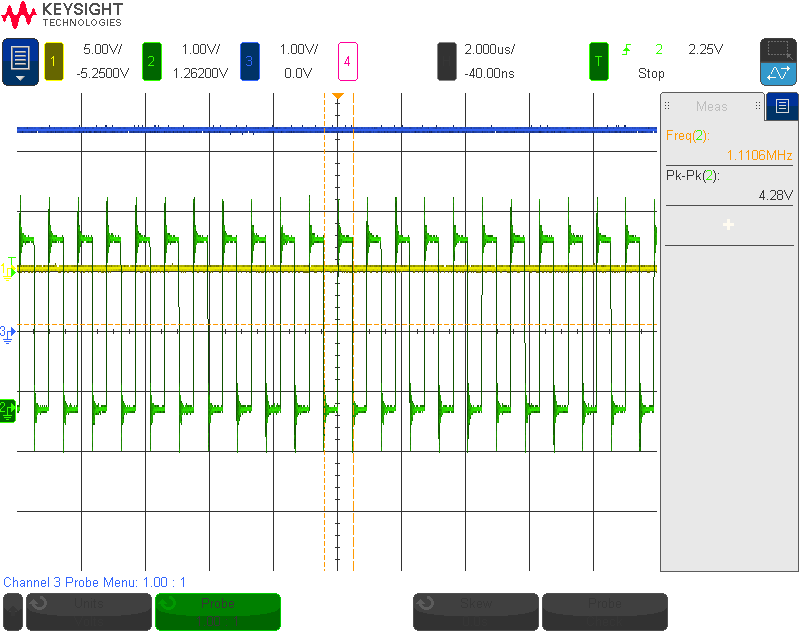
\includegraphics[width=0.9\textwidth, trim=0mm 21mm 0mm 11mm, clip]{images/scopeShots/scope_0b.png}
    \caption{$VCO_{\mathrm{out}}$ zoomed in, Parameter in Listing \ref{lst:meas:scope:0}}
    \label{fig:meas:scope:0}
\end{figure}

\begin{figure}[h!tb]
    \centering
    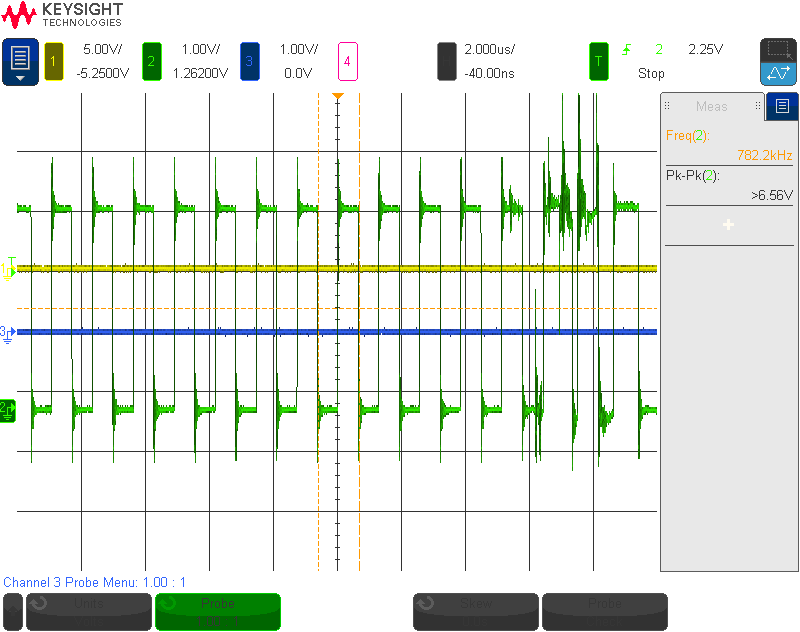
\includegraphics[width=0.9\textwidth, trim=0mm 21mm 0mm 11mm, clip]{images/scopeShots/scope_1b.png}
    \caption{$VCO_{\mathrm{out}}$ mit St\"orungen, Parameter in Listing \ref{lst:meas:scope:1}}
    \label{fig:meas:scope:1}
\end{figure}

\begin{figure}[h!tb]
    \centering
    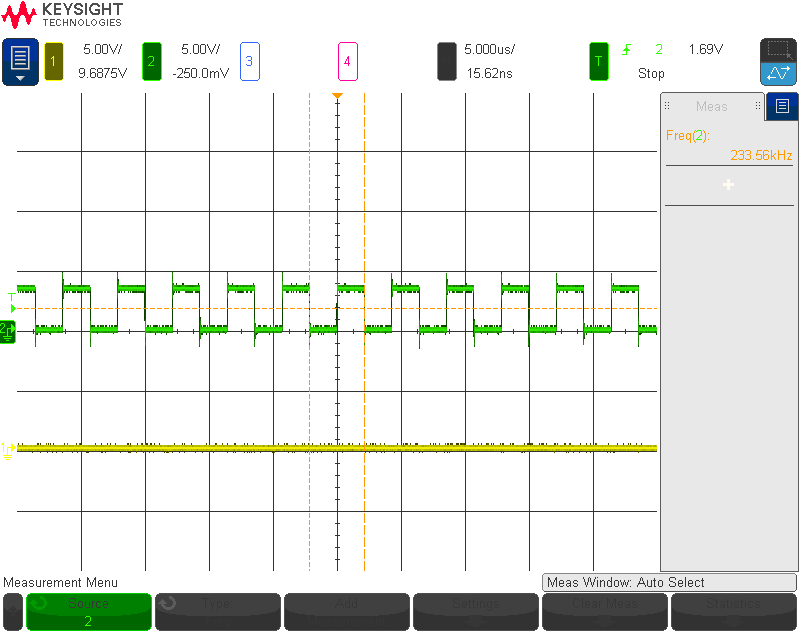
\includegraphics[width=0.9\textwidth, trim=0mm 21mm 0mm 11mm, clip]{images/scopeShots/scope_6b.png}
    \caption{$VCO_{\mathrm{out}}$ zoomed out, Parameter in Listing \ref{lst:meas:scope:6}}
    \label{fig:meas:scope:6}
\end{figure}


% ---------------------------------------------------------------------------- %
\clearpage
\section{Demodulator}
\label{sec:val:demodulator}
% ---------------------------------------------------------------------------- %

Beim  Demodulator  ist  es   wichtig,  dass  die  Schaltflanken  einigermassen
Steil  sind  und   der  Signalverlauf  ansonsten  konstant.    Dass  dies  der
Fall ist,  kann den Abbildungen~\ref{fig:meas:scope:7},~\ref{fig:meas:scope:8}
und~\ref{fig:meas:scope:9} entnommen  werden.  Man sieht, dass  die Schaltzeit
etwa  \SI{2}{\micro\second} betr\"agt. Wenn  man nun  mit 9600  Baud empfangen
w\"urde, erg\"abe dies eine Periode von \SI{104}{\micro\second}.  Damit w\"are
die Schaltzeit lediglich  3.8 Prozent, was reibungslos  funktioniert, wie auch
gut in  Grafik \ref{fig:meas:scope:8} zu  erkennen ist.  Ein Problem,  was auf
den Grafiken  gut sichtbar ist,  ist die geringe Amplitude. Dem  wird mithilfe
eines Verst\"arkers entgegengewirkt, welcher die Signalamplitude verdoppelt.

\vspace*{7em}
\begin{figure}[h!tb]
    \centering
    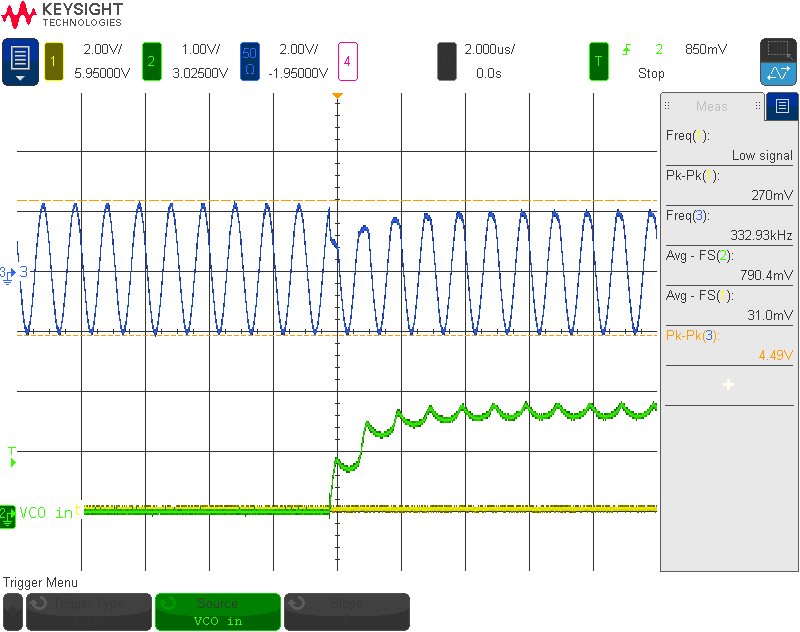
\includegraphics[width=0.9\textwidth, trim=0mm 21mm 0mm 11mm, clip]{images/scopeShots/scope_7b.png}
    \caption{Steigende Flanke des Demodulators, Parameter in Listing \ref{lst:meas:scope:7}}
    \label{fig:meas:scope:7}
\end{figure}

\begin{figure}[h!tb]
    \centering
    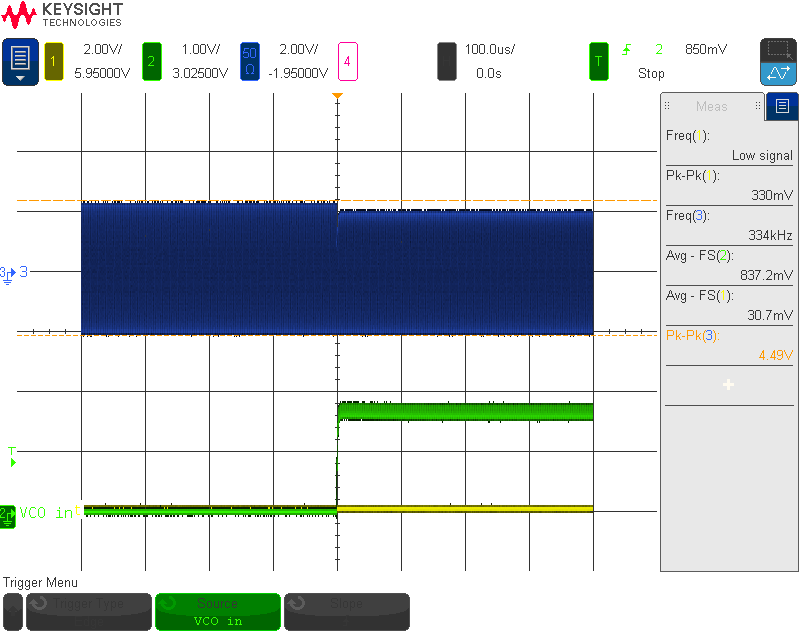
\includegraphics[width=0.9\textwidth, trim=0mm 21mm 0mm 11mm, clip]{images/scopeShots/scope_8b.png}
    \caption{Steigende Flanke des Demodulators im Makroskopischen, Parameter in Listing \ref{lst:meas:scope:8}}
    \label{fig:meas:scope:8}
\end{figure}

\begin{figure}[h!tb]
    \centering
    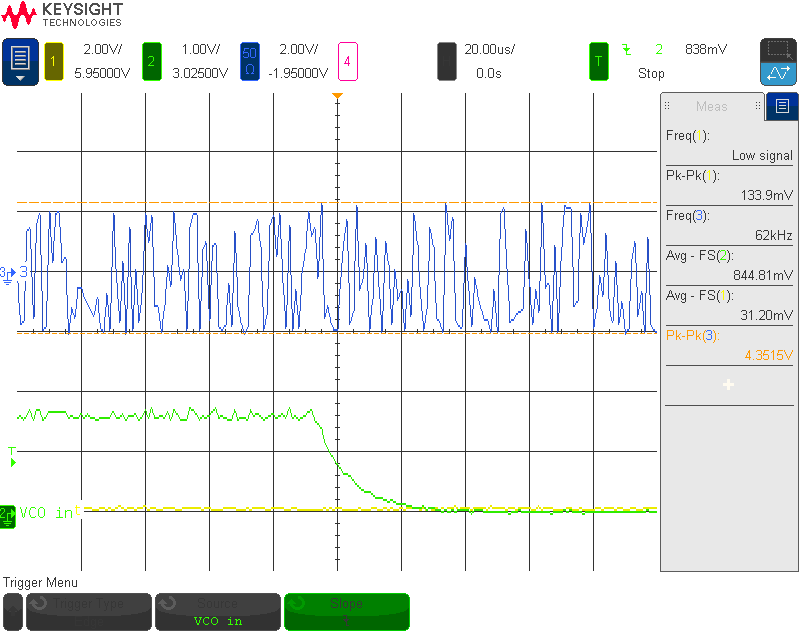
\includegraphics[width=0.9\textwidth, trim=0mm 21mm 0mm 11mm, clip]{images/scopeShots/scope_9b.png}
    \caption{Steigende Flanke  des Demodulators, Parameter in Listing \ref{lst:meas:scope:9}}
    \label{fig:meas:scope:9}
\end{figure}


% ---------------------------------------------------------------------------- %
\clearpage
\section{Gesamtsystem}
\label{sec:validierung:total}
% ---------------------------------------------------------------------------- %

Wie  in den  vorherigen Abschnitten  dokumentiert ist,  sind alle  Teilsysteme
getestet und  funktionst\"uchtig.  Am Sensorboard m\"ussen  einige Anpassungen
zum Einstellen der Tr\"agerfrequenz der OOSK gemacht werden. Des Weiteren muss
am Demodulator der  Verst\"arker in Betrieb genommen werden, da  im Moment die
empfangene  Signalamplitude zu  klein  ist, ansonsten  aber  in Ordnung.   Die
Modulation und Demodulation  sind separat getestet. Nun ist  es wichtig, diese
im  Zusammenspiel zu  testen. Dank ansonsten  funktionst\"uchtigem Sensorboard
mit kompletter Firmware sollte dies einfach m\"oglich sein.

Beim Master sieht  die Lage \"ahnlich aus. Bis auf die  Strommessung sind alle
Teilkomponenten  erfolgreich getestet. Diese  m\"ussten  jetzt im  Vollbetrieb
validiert werden, da dies Aufgrund fehlender Kommunikation der Sensoren bisher
weggefallen ist.

Softwareseitig   ist  der   Master   auf  gutem   Wege.    Das  Auslesen   und
Auswerten  der  Sensoren  ist  \"uber eine  normale  UART-Verbindung  getestet
und  funktioniert. Das  GUI wird  angesteuert  und  eine  Fehlermeldung  wird
ausgel\"ost,  wenn  ein  Modul  defekt   ist.   Jedoch  fehlt  ein  wenig  der
Feinschliff. So fehlt  noch die  Ansteuerungssoftware f\"ur  das GSM-Modul. Da
dieses  voll   integriert  ist,  kann   dies  angenehm  \"uber   ein  two-wire
Interface gemacht werden  und ist ein  einfacher Task, sobald  die restlichen
Teilsysteme  laufen.  Die  Ansteuerung der  Strommessung ist  entwickelt, aber
noch nicht getestet.  Zu guter Letzt  ist eine gute Abrundung wichtig. So muss
zum Beispiel noch der Button zum Ein- und Ausschalten des Displays angesteuert
werden.

% **************************************************************************** %
\chapter{Benutzerhandbuch}
\label{chap:userguide}
% **************************************************************************** %

\noindent\adjustbox{valign=t}{\begin{minipage}{44mm}
    
\includegraphics[width=29mm]{images/userguide/danger.png}\footnotemark
\end{minipage}}
\noindent\adjustbox{valign=t}{\begin{minipage}{95mm}
    Wichtiger    Hinweis: Die    Installation    und    Inbetriebnahme    darf
    ausschliesslich  durch  eine  autorisierte  Elektrofachkraft  ausgef\"uhrt
    werden. Bei der  Installation des Systems  ist zwingend zu  beachten, dass
    Teile  der Photovoltaikanlage  st\"andig unter  Spannung stehen  k\"onnen,
    auch bei abgeschalteter Anlage.
\end{minipage}}
\footnotetext{
    Bildquelle: \cite{ref:danger}
}

% ---------------------------------------------------------------------------- %
\section{Installation und Inbetriebnahme}
\label{sec:userguide:installation}
% ---------------------------------------------------------------------------- %

Die Installation des Master-Ger\"ates erfolgt im Generatoranschlusskasten. Das
Master-Geh\"ause  wird  auf  einer  Hutschiene  platziert  und  innerhalb  des
GAKs  mit  \SI{230}{\volt}  AC  gespeist. Die DC-Leitungen  von  bis  zu  drei
Str\"angen pro  \Master~ werden auf die  daf\"ur vorgesehenen Anschlussklemmen
gef\"uhrt. Der   maximale    Leiterquerschnitt   der    DC-Leitung   betr\"agt
\SI{4}{\milli\meter\squared}  und  ist   f\"ur  g\"angige  Photovoltaikanlagen
ausreichend.

Um eine  einwandfreie Alarmierung im  Fehlerfall zu gew\"ahrleisten,  wird die
Installation  mindestens eines  externen  Meldeger\"ats empfohlen. \"Uber  die
beiden Relaiskontakte  am Master-Ger\"at  k\"onnen externe Ger\"ate  mit einer
Nennspannung bis max. \SI{250}{\volt} geschaltet werden.

Nach der  Installation und dem  Einschalten des Master-Ger\"ates   erfolgt die
Installation  der Sensorkomponenten. Jedes  PV-Modul  wird im    zugeh\"origen
Anschlusskasten  mit einem  Sensor  ausgestattet. Der Sensor  wird \"uber  die
beiden  Kupferdr\"ahte  der  Platine  an den  Anschlussklemmen  des  PV-Moduls
angeschlossen. Dabei  ist die  richtige  Polarit\"at  zu beachten. Sobald  der
Sensor mit der DC Leitung verbunden ist, wird die Seriennummer automatisch vom
Master-Ger\"at erfasst  und ins System integriert. Jeder  Sensor besitzt dabei
eine einzigartige  Seriennummer. Diese Seriennummer wird  jeweils zus\"atzlich
in  Form eines  Klebstreifens  mit dem  Sensor  mitgeliefert. Um den  Standort
jedes  Sensors  zu dokumentieren,  sind  die  Klebstreifen im  Anlageplan  auf
dem  jeweiligen Modul  aufzutragen. Gleiches Vorgehen  f\"ur die  Installation
weiterer Sensoren.   Ist ein  Sensor defekt, kann  die gesamte  Platine bequem
ausgetauscht  werden. Die   neue  Seriennummer  wird  dabei   automatisch  vom
Master-Ger\"at erfasst und ins System  integriert. Dabei ist zu beachten, dass
der Anlageplan mit den Seriennummern-Klebstreifen stets angepasst wird.


% ---------------------------------------------------------------------------- %
\section{Regul\"arer Betrieb}
\label{sec:userguide:regular}
% ---------------------------------------------------------------------------- %

\enlargethispage{2em}
S\"amtliche  Einstellungen des  Systems  werden \"uber  das Touch-Display  des
Master-Ger\"ates get\"atigt. Im regul\"aren Betrieb sind \"ublicherweise keine
Einstellungen vorzunehmen. Der  Gr\"une Knopf,  rechts vom Display,  dient zum
Aus- bzw. Einschalten des Displays. Im  regul\"aren Betrieb empfiehlt es sich,
aus energietechnischen Gr\"unden das Display ausgeschaltet zu lassen.

\begin{wrapfigure}{r}{0.475\textwidth}
    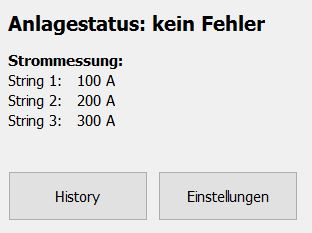
\includegraphics[width=0.475\textwidth]{images/userguide/screen0.png}
    \caption{Hauptmenu}
    \label{fig:userguide:screen0}
\end{wrapfigure}

Bei Bet\"atigung des gr\"unen Knopfes  erscheint das Hauptmenu, dargestellt in
Abbildung \ref{fig:userguide:screen0}. Dieses dient  einerseits zur Auflistung
aktueller  Messwerte der  Strangstr\"ome  und  des Anlagestatus,  andererseits
f\"uhrt  es mittels  weiterer  Buttons in  die  jeweiligen Untermenus. In  der
obersten Zeile  \emph{Anlagestatus} wird  dargestellt, ob  ein Problem  an der
Anlage vorliegt. Wird bei Anlagestatus  \emph{kein Fehler} angezeigt, liegt an
der  Anlage keine  St\"orung vor. Wird  jedoch die  Fehlfunktion eines  Moduls
detektiert,  erfolgt  eine Meldung  im  Hauptmenu  (weitere Informationen  zum
St\"orbetrieb im folgenden Kapitel).

\vspace*{3em}
\noindent\adjustbox{valign=t}{\begin{minipage}{0.475\textwidth}
    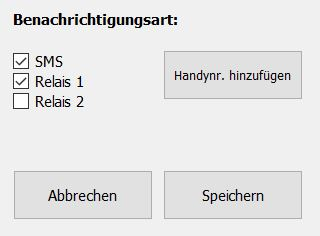
\includegraphics[width=\textwidth]{images/userguide/screen1.png}
    \figcaption[Master: Menu: Einstellungen]{Einstellungen}
    \label{fig:userguide:screen1}
\end{minipage}}
\hspace*{0.04\textwidth}
\noindent\adjustbox{valign=t}{\begin{minipage}{0.475\textwidth}
    \includegraphics[width=\textwidth]{images/userguide/screen2.png}
    \figcaption[Master: Menu: Einstellungen: Telefonnummer]{Eingabe einer Telefonnummer}
    \label{fig:userguide:screen2}
\end{minipage}}

Im     Untermenu     \emph{Einstellungen},    dargestellt     in     Abbildung
\ref{fig:userguide:screen1},   k\"onnen  die   SMS-Benachrichtigung  und   die
Relaisausg\"ange konfiguriert werden. Beim  Hinzuf\"ugen einer Handynummer mit
korrekter Vorwahl  (Bsp. \code{0041 79  612 33  22}) und bei  Bet\"atigung des
entsprechenden K\"astchens  wird automatisch  die Benachrichtigung  \"uber SMS
aktiviert. Das zugeh\"orige Menu  ist in Abbildung \ref{fig:userguide:screen2}
gezeigt.  Analog werden  die beiden Relais bei der  Aktivierung des jeweiligen
K\"astchens  aktiviert.    \"Uber  den  Button  \emph{Speichern}   werden  die
Einstellungen im System \"ubernommen.


% ---------------------------------------------------------------------------- %
\section{St\"orbetrieb}
\label{sec:userguide:errors}
% ---------------------------------------------------------------------------- %

Wird die Fehlfunktion eines  Moduls detektiert, erfolgt eine St\"orungsmeldung
an das  Master-Ger\"at. Folglich erscheint  im Hauptmenu  des Master-Ger\"ates
die  Seriennummer des  entsprechenden Moduls  wie auch  Datum und  Uhrzeit der
Fehlererkennung, wie in Abbildung \ref{fig:userguide:screen3} gezeigt.

Zeitgleich  werden  am  Master-Ger\"at  zwei  Relaiskontakte  bet\"atigt,  die
f\"ur externe  akustische oder  optische Meldeger\"ate  vorgesehen sind. Diese
externen Meldeger\"ate lassen sich mit  dem entsprechenden Button im Hauptmenu
quittieren. Sofern  unter  \emph{Einstellungen}  eine  Handynummer  hinterlegt
worden   ist,  erfolgt   zus\"atzlich  eine   Fehlerbenachrichtigung  an   das
entsprechende Mobiltelefon.

Um Energieverluste  zu minimieren,  sollte bei  einem Fehlerfall  umgehend ein
Installateur der Photovoltaikanlage konsultiert werden. Sobald das fehlerhafte
Modul wieder einwandfrei funktioniert, wird die Fehlermeldung im Hauptmenu des
Master-Ger\"ates  automatisch ausgeblendet. Im  Untermenu \emph{Fehlerverlauf}
(Abbildung \ref{fig:userguide:screen4})  sind alle  bisherigen Fehlermeldungen
der Anlage ersichtlich.

\vspace*{3em}
\noindent\adjustbox{valign=t}{\begin{minipage}{0.475\textwidth}
    \includegraphics[width=\textwidth]{images/userguide/screen3.png}
    \figcaption[Master: Menu: Modulfehler]{Fehler bei einem Modul}
    \label{fig:userguide:screen3}
\end{minipage}}
\hspace*{0.04\textwidth}
\noindent\adjustbox{valign=t}{\begin{minipage}{0.475\textwidth}
    \includegraphics[width=\textwidth]{images/userguide/screen4.png}
    \figcaption[Master: Menu: Einstellungen: Fehlerverlauf]{Fehlerverlauf der Anlage}
    \label{fig:userguide:screen4}
\end{minipage}}

% **************************************************************************** %
\chapter{Fazit}
\label{chap:fazit}
% **************************************************************************** %
\enlargethispage{4em}

\vspace*{-2em}
Nach  Abschluss  des   Projektes  steht  dem  Auftraggeber   ein  Produkt  zur
Verf\"ugung, das  als Gesamtsystem die  Spannungen an PV-Modulen  erfassen und
auswerten  kann. Die einzelnen  Teilsysteme sind  mehrheitlich als  Prototypen
vorhanden, im Labor getestet und funktionsf\"ahig.

Der  Sensor kann  Spannungen messen  und Werte  ausgeben. Mit einer  Abmessung
von  knapp  $\SI{5}{\centi\meter}\times\SI{5}{\centi\meter}$  bieten  wir  dem
Auftraggeber eine  Sensorplatine, die  garantiert in  jedem Anschlussgeh\"ause
Platz findet. Die  Firmware zusammen  mit den  gew\"ahlten Hardwarekomponenten
erm\"oglichen eine saubere Messung  der Modulspannung. Die Hauptproblematik im
Projekt bestand darin, eine optimale L\"osung f\"ur die Kommunikation zwischen
Sensor und Master-Ger\"at  zu finden. Mit induktiver Einkopplung  und OOSK ist
eine eine Variante gew\"ahlt worden, die es erm\"oglicht, die gemessenen Daten
der  PV-Module dem  Masterger\"at  zu  \"ubermitteln. Das Grundprinzip  dieser
\"Ubertragungsmethode ist validiert.

Mit einem Testaufbau k\"onnen Signale  vom Master-Ger\"at empfangen und an den
Raspberry  Pi  weitergeleitet  werden. Mithilfe  der  Mastersoftware  ist  der
Raspberry Pi  im Stande, die  empfangenen Messwerte, auszuwerten,  mit anderen
Messdaten zu vergleichen und n\"otigenfalls eine Fehlermeldung auf dem Display
auszugeben. Das  Master-Ger\"at  bietet  einerseits  eine  benutzerfreundliche
Oberfl\"ache,  andererseits l\"asst  sich  das schlichte  Geh\"ause bequem  in
einen bestehenden  Generatoranschlusskasten installieren, auch wenn  nur wenig
Platz  vorhanden  ist. Die  Bedienung  und  Inbetriebnahme  \"uber  das  2.5``
Touch-Display ist \"ausserst komfortabel und selbsterkl\"arend.  Ein GSM-Modul
f\"ur  das Versenden  einer Textnachricht  an ein  Mobiltelefon ist  ebenfalls
vorhanden,  lediglich  dessen  Ansteuerungsfirmware  muss  noch  implementiert
werden. Anschliessend  ist  das  Master-Ger\"at  im  Stande,  im  Falle  eines
Modulfehlers,  neben der  Bet\"atigung  der beiden  Relaiskontakte, auch  eine
Fehlermeldung per  SMS zu  versenden. Die geplante Zusatzfunktion  zur Messung
der Strangstr\"ome am Master-Ger\"at ist wegen Zeitmangel noch nicht getested,
jedoch in die Entwicklung integriert.

Als  n\"achster   Schritt  sollte  die  Daten\"ubermittlung   vom  Sensor  zum
Master-Ger\"at mittels  Powerline getestet werden, wie  auch das Zusammenspiel
von Tochterboard und  Raspberry Pi. Letztlich sollte das  gesamten Systems als
Ganzes \"uberpr\"uft werden.



% -------------------------------------------------------- %
% Appendices are  usually numbered  and therefore  part of %
% the mainmatter, not the backmatter.                      %
% The advice about meaningful chapter names applies to the %
% appendices as well, see above.                           %
% -------------------------------------------------------- %
\appendixpage
\appendix
% **************************************************************************** %
\chapter{Daten von Solarmodulen}
\label{app:commercial:modules}
% **************************************************************************** %

Dieser Abschnitt enth\"alt in  Tabelle \ref{tab:moduleData:IU} einige Eckdaten
von kommerziell  erh\"altlichen Modulen  mit den  zugeh\"origen Quellen. Diese
Informationen sollen  prim\"ar als Anhaltspunkt und  Vergleich zwischen Praxis
und unseren Simuationen dienen.

\begin{table}
    \centering
    \small
    \caption{%
        Daten   f\"ur   Solarmodule.  \textbf{pk}:   polykristallines   Panel,
        \textbf{mk}:     monokristallines     Panel.     \emph{Anmerkung}: Die
        Konfiguration  der Module  (wieviele  Zellen in  Serie  und wie  viele
        Str\"ange  parallel)  ist  mit   Ausnahme  des  Solarex  MSX-60  nicht
        angegeben. Es  ist  aber  bekannt,  in  welcher  Gr\"ossenordnung  die
        Spannung  pro  Zelle  ungef\"ahr  liegen sollte,  womit  man  aus  den
        angegebenen Leerlaufspannungen  und der Gesamtzahl der  Zellen auf die
        Konfiguration eines Modules schliessen kann.%
    }
    \label{tab:moduleData:IU}
    \begin{tabular}{lp{20mm}lllll}
        \toprule
          \rotatebox{70}{\pbox{25mm}{Quelle}}
        & \rotatebox{70}{\pbox{25mm}{Modell}}
        & \rotatebox{70}{\pbox{25mm}{Kurzschluss-\\strom $I_{\mathrm{SC}}$}}
        & \rotatebox{70}{\pbox{25mm}{Leerlauf-\\spannung $V_{\mathrm{OC}}$}}
        & \rotatebox{70}{\pbox{25mm}{Anzahl Zellen \\(total)}}
        & \rotatebox{70}{\pbox{25mm}{Anzahl Zellen \\(Strang)}}
        & \rotatebox{70}{\pbox{25mm}{Leerlaufspan-\\nung pro Zelle}} \\
        \midrule

          \cite{ref:solar:bonkoungou}
        & Solarex MSX-60
        & \SI{3.8}{\ampere}
        & \SI{21.1}{\volt}
        & \num{36}
        & \num{36}
        & \SI{586}{\milli\volt}
        \\

          \cite{ref:solar:px85}
        & Sunset PX85 (\textbf{pk})
        & \SI{5.5}{\ampere}
        & \SI{21.5}{\volt}
        & \num{76}
        & \num{38}
        & \SI{566}{\milli\volt}
        \\

          \cite{ref:solar:as150}
        & Sunset Solargenerator AS150 (\textbf{mk})
        & \SI{8.7}{\ampere}
        & \SI{22.3}{\volt}
        & \num{36}
        & \num{36}
        & \SI{620}{\milli\volt}
        \\

          \cite{ref:solar:sunmodulePro}
        & Sunmodule Pro-Series XL SW320 (\textbf{mk})
        & \SI{9.41}{\ampere}
        & \SI{45.9}{\volt}
        & \num{72}
        & \num{72}
        & \SI{638}{\milli\volt}
        \\

        \bottomrule
    \end{tabular}
\end{table}


%\begin{table}[h!tb]
%    \centering
%    \caption{Abmessungen der Solarmodule aus Tabelle \ref{tab:moduleData:IU}}
%    \label{tab:moduleData:Dimensions}
%    \begin{tabular}{lp{20mm}ll}
%        \toprule
%          \rotatebox{70}{\pbox{25mm}{Quelle}}
%        & \rotatebox{70}{\pbox{25mm}{Modell}}
%        & \rotatebox{70}{\pbox{25mm}{Abmessungen Modul ($\si{\milli\meter} \si{\milli\meter}$)}}
%        & \rotatebox{70}{\pbox{25mm}{Abmessungen Zelle ($\si{\milli\meter} \si{\milli\meter}$)}} \\
%        \midrule
%
%          \cite{ref:solar:px85}
%        & Sunset PX85 (\textbf{pk})
%        & $1477 \times 660$
%        & $\approx 165 \times 75$
%        \\
%
%          \cite{ref:solar:as150}
%        & Sunset Solargenerator AS150 (\textbf{mk})
%        & $1480 \times 660$
%        & $\approx 155 \times 164$
%        \\
%
%          \cite{ref:solar:sunmodulePro}
%        & Sunmodule Pro-Series XL SW320 (\textbf{mk})
%        & $1985 \times 990$
%        & $156 \times 156$
%        \\
%        \bottomrule
%    \end{tabular}
%\end{table}

% **************************************************************************** %
\chapter{\code{LTspice}-Schaltungen}
\label{app:ltspice}
% **************************************************************************** %

Dieses Kapitel  beinhaltet \code{LTspice}-Schaltungen, welche  zu Simulationen
benutzt  worden  sind. Erkl\"arungen zu  den  jeweiligen  Schaltungen sind  in
den  Kapiteln zu  finden, welche  auf  sie verweisen. Zu  jeder Schaltung  ist
angegeben, wo sie auf dem Datentr\"ager gefunden werden kann.

\noindent\begin{minipage}{\textwidth}
    \centering
    \includegraphics[width=0.9\textwidth]{images/ltspice/generic-iv-curves/cell.eps}
    \figcaption[\code{LTspice}-Schaltung f\"ur PV-Zelle]{%
        Modell   der   PV-Zelle,   aus   welchem  das   Modul   in   Abbildung
        \ref{fig:ltspice:iv:generic:module}  aufgebaut  ist. Die  Simulationen
        aus   Abbildung   \ref{fig:simu:iv-curves:module:generic}  auf   Seite
        \pageref{fig:simu:iv-curves:module:generic}   basieren    auf   diesem
        Modell. Gegen\"uber   dem   in   Abschnitt   \ref{sec:simu:model:cell}
        hergeleiteten Modell hat dieses  Modell einen h\"oheren Photostrom und
        einen niedrigeren Shunt-Widerstand. Dies  erzeugt etwas anschaulichere
        Kurven.\protect\\
        Dateipfad: \code{ltspice/generic/cell-9A.asc}%
    }
    \label{fig:ltspice:iv:generic:cell}
    \includegraphics[width=0.9\textwidth]{images/ltspice/jac/cell.eps}
    \figcaption[\code{LTspice}-Schaltung f\"ur PV-Zelle]{%
        Modell  der   PV-Zelle,  auf  welchen  die   Simulationen  in  Kapitel
        \ref{chap:simu} ab  Seite \pageref{chap:simu}  beruhen. Die Herleitung
        ist in Abschnitt \ref{sec:simu:model:cell} dokumentiert.\protect\\
        Dateipfad: \code{ltspice/jac/jac-cell.asc}%
    }
    \label{fig:ltspice:jac:cell}
\end{minipage}

\clearpage
\begin{figure}[h!tb]
    \centering
    \begin{tikzpicture}[%
        spy scope = {magnification=7,size=25*8,connect spies},
        every spy on node/.style={circle,red,draw},
        every spy in node/.style = {circle, fill=white, fill opacity=1, draw},
        ]
        \node[inner sep = 0pt,anchor=south west] {%
            \includegraphics[width=\textwidth]{images/ltspice/generic-iv-curves/module.eps}
        };
        \spy[red] on (0.45,1.2) in node at (10,8);
    \end{tikzpicture}
    \caption[\code{LTspice}-Schaltung f\"ur PV-Modul f\"ur IV- und PV-Kurven]{%
        \code{LTspice}-Modell,    welches    zur    Erzeugung    der    Kurven
        in   Abbildung   \ref{fig:simu:iv-curves:module:generic}   auf   Seite
        \pageref{fig:simu:iv-curves:module:generic}  benutzt  worden  ist. Das
        Modell  der Zelle,  aus welcher  dieses  Modul aufgebaut  ist, ist  in
        Abbildung \ref{fig:ltspice:iv:generic:cell} abgebildet.\protect\\
        Dateipfad: \code{ltspice/generic/module-9A.asc}%
    }
    \label{fig:ltspice:iv:generic:module}
\end{figure}

\clearpage
Bei  \hfill Schaltungen  mit \hfill  hunderten oder  gar tausenden  \hfill von
Komponenten  wird\\ \code{LTspice}  sehr schwerf\"allig  zum Bedienen,  da das
Updaten der  Netlist sehr lange  dauert und  die Netlist bei  jeder \"Anderung
der  Schaltung  aktualisiert  werden  muss.  Zur  einfacheren  Handhabung  von
Simulationen  mit mehreren  Modulen wird  deshalb ein  neues Symbol  f\"ur ein
Modul definiert, gezeigt in Abbildung \ref{fig:ltspice:module:symbol}, welches
je nach Bedarf  mit der Schaltung f\"ur ein Modul  mit oder ohne Freilaufdiode
verkn\"upft werden kann.

\begin{figure}[h!tb]
    \centering
    \includegraphics[width=0.4\textwidth]{images/ltspice/module-symbol.eps}
    \caption{%
        Selbst erstelltes Symbol f\"ur PV-Modul\protect\\
        Dateipfad:   \code{ltspice/jac/jacModule.asy}   (mit   Freilaufdioden,
        verkn\"upft          mit          Modul         aus          Abbildung
        \ref{fig:ltspice:jacModule:NoDiode})\protect\\
        Dateipfad: \code{ltspice/jac/jacModuleNoD.asy} (ohne Freilaufdioden, verknupft mit
        Modul aus Abbildung \ref{fig:ltspice:jacModule:Diode})%
    }
    \label{fig:ltspice:module:symbol}
\end{figure}

\begin{figure}[h!tb]
    \centering
    \includegraphics[width=\textwidth]{images/ltspice/jac/stringNoD.eps}
    \caption[\code{LTspice}-Schaltung f\"ur Modulstrang]{%
        \code{LTspice}-Schaltung  f\"ur  einen   Modulstrang  aus  20  Modulen
        und   variablem  Lastwiderstand   \code{Rload}   zur  Erstellung   von
        Strom-Spannungs-Kurven. Es  wird   je  ein  Strang  aus   Modulen  mit
        Freilaufdiode   (Abbildung  \ref{fig:ltspice:jacModule:NoDiode})   und
        ohne   Freilaufdiode   (Abbildung   \ref{fig:ltspice:jacModule:Diode})
        simuliert.\protect\\
        Dateipfad: \code{ltspice/jac/string.asc} (mit Freilaufdioden)\protect\\
        Dateipfad: \code{ltspice/jac/stringNoD.asc} (ohne Freilaufdioden)%
    }
    \label{fig:ltspice:string:ivCurve}
\end{figure}

\begin{figure}[h!tb]
    \centering
    \begin{tikzpicture}[%
        spy scope = {magnification=5,height=25*5.5,width=25*10,connect spies},
        every spy on node/.style={rectangle,red,draw},
        every spy in node/.style = {rectangle,fill=white, fill opacity=1, draw},
        ]
        \node[inner sep = 0pt,anchor=south west] {%
            \includegraphics[width=\textwidth]{images/ltspice/jac/jacModuleNoD.eps}
        };
        \spy[red] on (1.15,1.13) in node at (9,8);
    \end{tikzpicture}
    \caption[\code{LTspice}-Schaltung f\"ur PV-Modul ohne Freilaufdiode]{%
        Modul    ohne   Freilaufdiode,    benutzt    f\"ur   die    Simulation
        aus   Abbildung   \ref{fig:simu:iv-curves:array:generic}   von   Seite
        \pageref{fig:simu:iv-curves:array:generic}.\protect\\
        Dateipfad: \code{ltspice/jac/jacModuleNoD.asc}%
    }
    \label{fig:ltspice:jacModule:NoDiode}
\end{figure}

\begin{figure}[h!tb]
    \centering
    \begin{tikzpicture}[%
        spy scope = {magnification=5,height=25*5.5,width=25*10,connect spies},
        every spy on node/.style={red,draw},
        every spy in node/.style = {fill=white, fill opacity=1, draw},
        ]
        \node[inner sep = 0pt,anchor=south west] {%
            \includegraphics[width=\textwidth]{images/ltspice/jac/jacModule.eps}
        };
        \spy[rectangle,red] on (1.15,1.13) in node at (9,8);
        \spy[circle,size=25*3,red] on (7.05,0.9) in node at (9,3);
    \end{tikzpicture}
    \caption[\code{LTspice}-Schaltung f\"ur PV-Modul mit Freilaufdiode]{%
        Modul      mit      Freilaufdiode       (unten,      Mitte,      Diode
        \code{D145}). Benutzt       f\"ur       die       Simulation       aus
        Abbildung   \ref{fig:simu:iv-curves:array:generic:bypass}  von   Seite
        \pageref{fig:simu:iv-curves:array:generic:bypass}       sowie      die
        Simulationen zu den L\"osungsvarianten in Abschnitt
        \ref{sec:simu:coupling:inductive} ab Seite
        \pageref{sec:simu:coupling:inductive}, Abschnitt
        \ref{sec:simu:coupling:capacitive} ab Seite
        \pageref{sec:simu:coupling:capacitive} und Abschnitt
        \ref{sec:simu:short} ab Seite
        \pageref{sec:simu:short}.
        Abbildung   \ref{fig:ltspice:jac:cell}    enth\"alt   das   verwendete
        Zellenmodell.\protect\\
        Dateipfad: \code{ltspice/jac/jacModule.asc}%
    }
    \label{fig:ltspice:jacModule:Diode}
\end{figure}

% **************************************************************************** %
\chapter{Schemata}
\label{app:chap:schemas}
% **************************************************************************** %
{\begin{a3pages}

\begin{tikzpicture}[remember picture,overlay]
    \node[inner sep=0pt] at (current page.center) {%
        \includegraphics{images/sensor-sch/sensor--sch.eps}%
    };
\end{tikzpicture}
\figcaption{Schema Sensor}
\label{fig:schema:sensor:full}


\clearpage
\begin{tikzpicture}[remember picture,overlay]
    \node[inner sep=0pt] at (current page.center) {%
        \includegraphics{images/superv-sch/supervisor--sch.eps}%
    };
\end{tikzpicture}
\vspace{155mm}
\figcaption{Schema Master}
\label{fig:schema:master:full}

\end{a3pages}}

% **************************************************************************** %
\chapter{Zusatzinformationen Validierung}
\label{app:validation}
% **************************************************************************** %

Es  sind an  dieser  Stelle  zus\"atzliche Messergebnisse  und  die f\"ur  das
Oszilloskop benutzten Einstellungen aufgef\"uhrt.

% ---------------------------------------------------------------------------- %
\clearpage
\section{Zus\"atzliche Plots f\"ur Validierung}
% ---------------------------------------------------------------------------- %

Es  sind  hier der  Verlauf  des  Seriewiderstands  unserer Spule  \"uber  die
Frequenz und der Power Choke Test in Abh\"angigkeit des Flusses aufgef\"uhrt.

\begin{figure}[h!tb]
    \centering
    %% Creator: Matplotlib, PGF backend
%%
%% To include the figure in your LaTeX document, write
%%   \input{<filename>.pgf}
%%
%% Make sure the required packages are loaded in your preamble
%%   \usepackage{pgf}
%%
%% Figures using additional raster images can only be included by \input if
%% they are in the same directory as the main LaTeX file. For loading figures
%% from other directories you can use the `import` package
%%   \usepackage{import}
%% and then include the figures with
%%   \import{<path to file>}{<filename>.pgf}
%%
%% Matplotlib used the following preamble
%%   \usepackage{fontspec}
%%   \setmainfont{Bitstream Vera Serif}
%%   \setsansfont{Bitstream Vera Sans}
%%   \setmonofont{Bitstream Vera Sans Mono}
%%
\begingroup%
\makeatletter%
\begin{pgfpicture}%
\pgfpathrectangle{\pgfpointorigin}{\pgfqpoint{5.500000in}{2.000000in}}%
\pgfusepath{use as bounding box, clip}%
\begin{pgfscope}%
\pgfsetbuttcap%
\pgfsetmiterjoin%
\pgfsetlinewidth{0.000000pt}%
\definecolor{currentstroke}{rgb}{0.000000,0.000000,0.000000}%
\pgfsetstrokecolor{currentstroke}%
\pgfsetstrokeopacity{0.000000}%
\pgfsetdash{}{0pt}%
\pgfpathmoveto{\pgfqpoint{0.000000in}{0.000000in}}%
\pgfpathlineto{\pgfqpoint{5.500000in}{0.000000in}}%
\pgfpathlineto{\pgfqpoint{5.500000in}{2.000000in}}%
\pgfpathlineto{\pgfqpoint{0.000000in}{2.000000in}}%
\pgfpathclose%
\pgfusepath{}%
\end{pgfscope}%
\begin{pgfscope}%
\pgfsetbuttcap%
\pgfsetmiterjoin%
\pgfsetlinewidth{0.000000pt}%
\definecolor{currentstroke}{rgb}{0.000000,0.000000,0.000000}%
\pgfsetstrokecolor{currentstroke}%
\pgfsetstrokeopacity{0.000000}%
\pgfsetdash{}{0pt}%
\pgfpathmoveto{\pgfqpoint{0.550000in}{0.400000in}}%
\pgfpathlineto{\pgfqpoint{5.225000in}{0.400000in}}%
\pgfpathlineto{\pgfqpoint{5.225000in}{1.800000in}}%
\pgfpathlineto{\pgfqpoint{0.550000in}{1.800000in}}%
\pgfpathclose%
\pgfusepath{}%
\end{pgfscope}%
\begin{pgfscope}%
\pgfpathrectangle{\pgfqpoint{0.550000in}{0.400000in}}{\pgfqpoint{4.675000in}{1.400000in}} %
\pgfusepath{clip}%
\pgfsetrectcap%
\pgfsetroundjoin%
\pgfsetlinewidth{0.501875pt}%
\definecolor{currentstroke}{rgb}{0.000000,0.000000,1.000000}%
\pgfsetstrokecolor{currentstroke}%
\pgfsetdash{}{0pt}%
\pgfpathmoveto{\pgfqpoint{0.550000in}{0.866669in}}%
\pgfpathlineto{\pgfqpoint{3.525728in}{0.867779in}}%
\pgfpathlineto{\pgfqpoint{3.832748in}{0.869913in}}%
\pgfpathlineto{\pgfqpoint{3.974449in}{0.872786in}}%
\pgfpathlineto{\pgfqpoint{4.068916in}{0.876596in}}%
\pgfpathlineto{\pgfqpoint{4.139767in}{0.881366in}}%
\pgfpathlineto{\pgfqpoint{4.187001in}{0.886332in}}%
\pgfpathlineto{\pgfqpoint{4.234235in}{0.893813in}}%
\pgfpathlineto{\pgfqpoint{4.257851in}{0.898885in}}%
\pgfpathlineto{\pgfqpoint{4.281468in}{0.900145in}}%
\pgfpathlineto{\pgfqpoint{4.305085in}{0.906640in}}%
\pgfpathlineto{\pgfqpoint{4.328702in}{0.914629in}}%
\pgfpathlineto{\pgfqpoint{4.352319in}{0.925171in}}%
\pgfpathlineto{\pgfqpoint{4.375936in}{0.938560in}}%
\pgfpathlineto{\pgfqpoint{4.399553in}{0.956650in}}%
\pgfpathlineto{\pgfqpoint{4.423170in}{0.983189in}}%
\pgfpathlineto{\pgfqpoint{4.446787in}{1.016029in}}%
\pgfpathlineto{\pgfqpoint{4.470403in}{1.065222in}}%
\pgfpathlineto{\pgfqpoint{4.494020in}{1.128892in}}%
\pgfpathlineto{\pgfqpoint{4.517637in}{1.212984in}}%
\pgfpathlineto{\pgfqpoint{4.541254in}{1.306962in}}%
\pgfpathlineto{\pgfqpoint{4.564871in}{1.378794in}}%
\pgfpathlineto{\pgfqpoint{4.588488in}{1.371648in}}%
\pgfpathlineto{\pgfqpoint{4.612105in}{1.301686in}}%
\pgfpathlineto{\pgfqpoint{4.635722in}{1.198242in}}%
\pgfpathlineto{\pgfqpoint{4.659339in}{1.119218in}}%
\pgfpathlineto{\pgfqpoint{4.682955in}{1.056679in}}%
\pgfpathlineto{\pgfqpoint{4.706572in}{1.010211in}}%
\pgfpathlineto{\pgfqpoint{4.730189in}{0.981949in}}%
\pgfpathlineto{\pgfqpoint{4.753806in}{0.956165in}}%
\pgfpathlineto{\pgfqpoint{4.777423in}{0.937728in}}%
\pgfpathlineto{\pgfqpoint{4.801040in}{0.925130in}}%
\pgfpathlineto{\pgfqpoint{4.848274in}{0.907150in}}%
\pgfpathlineto{\pgfqpoint{4.871891in}{0.898793in}}%
\pgfpathlineto{\pgfqpoint{4.919124in}{0.886171in}}%
\pgfpathlineto{\pgfqpoint{4.942741in}{0.869169in}}%
\pgfpathlineto{\pgfqpoint{4.966358in}{0.811600in}}%
\pgfpathlineto{\pgfqpoint{4.989975in}{0.504465in}}%
\pgfpathlineto{\pgfqpoint{5.013592in}{0.702752in}}%
\pgfpathlineto{\pgfqpoint{5.037209in}{0.817877in}}%
\pgfpathlineto{\pgfqpoint{5.060826in}{0.846062in}}%
\pgfpathlineto{\pgfqpoint{5.084443in}{0.856449in}}%
\pgfpathlineto{\pgfqpoint{5.108059in}{0.861238in}}%
\pgfpathlineto{\pgfqpoint{5.155293in}{0.865226in}}%
\pgfpathlineto{\pgfqpoint{5.235000in}{0.867323in}}%
\pgfpathlineto{\pgfqpoint{5.235000in}{0.867323in}}%
\pgfusepath{stroke}%
\end{pgfscope}%
\begin{pgfscope}%
\pgfpathrectangle{\pgfqpoint{0.550000in}{0.400000in}}{\pgfqpoint{4.675000in}{1.400000in}} %
\pgfusepath{clip}%
\pgfsetrectcap%
\pgfsetroundjoin%
\pgfsetlinewidth{0.501875pt}%
\definecolor{currentstroke}{rgb}{0.000000,0.500000,0.000000}%
\pgfsetstrokecolor{currentstroke}%
\pgfsetdash{}{0pt}%
\pgfpathmoveto{\pgfqpoint{0.550000in}{0.866676in}}%
\pgfpathlineto{\pgfqpoint{3.903598in}{0.867841in}}%
\pgfpathlineto{\pgfqpoint{4.187001in}{0.869638in}}%
\pgfpathlineto{\pgfqpoint{4.328702in}{0.872322in}}%
\pgfpathlineto{\pgfqpoint{4.399553in}{0.875129in}}%
\pgfpathlineto{\pgfqpoint{4.470403in}{0.879461in}}%
\pgfpathlineto{\pgfqpoint{4.517637in}{0.887437in}}%
\pgfpathlineto{\pgfqpoint{4.541254in}{0.893287in}}%
\pgfpathlineto{\pgfqpoint{4.564871in}{0.900962in}}%
\pgfpathlineto{\pgfqpoint{4.588488in}{0.913045in}}%
\pgfpathlineto{\pgfqpoint{4.612105in}{0.930602in}}%
\pgfpathlineto{\pgfqpoint{4.635722in}{0.958134in}}%
\pgfpathlineto{\pgfqpoint{4.659339in}{1.011542in}}%
\pgfpathlineto{\pgfqpoint{4.682955in}{1.098410in}}%
\pgfpathlineto{\pgfqpoint{4.706572in}{1.232497in}}%
\pgfpathlineto{\pgfqpoint{4.730189in}{1.326333in}}%
\pgfpathlineto{\pgfqpoint{4.753806in}{1.241580in}}%
\pgfpathlineto{\pgfqpoint{4.777423in}{1.106936in}}%
\pgfpathlineto{\pgfqpoint{4.801040in}{1.016290in}}%
\pgfpathlineto{\pgfqpoint{4.824657in}{0.965106in}}%
\pgfpathlineto{\pgfqpoint{4.848274in}{0.934464in}}%
\pgfpathlineto{\pgfqpoint{4.871891in}{0.916714in}}%
\pgfpathlineto{\pgfqpoint{4.895507in}{0.905498in}}%
\pgfpathlineto{\pgfqpoint{4.919124in}{0.897253in}}%
\pgfpathlineto{\pgfqpoint{4.966358in}{0.886935in}}%
\pgfpathlineto{\pgfqpoint{4.989975in}{0.884990in}}%
\pgfpathlineto{\pgfqpoint{5.013592in}{0.874948in}}%
\pgfpathlineto{\pgfqpoint{5.037209in}{0.764004in}}%
\pgfpathlineto{\pgfqpoint{5.060826in}{0.740414in}}%
\pgfpathlineto{\pgfqpoint{5.084443in}{0.841546in}}%
\pgfpathlineto{\pgfqpoint{5.108059in}{0.857035in}}%
\pgfpathlineto{\pgfqpoint{5.131676in}{0.862212in}}%
\pgfpathlineto{\pgfqpoint{5.178910in}{0.865782in}}%
\pgfpathlineto{\pgfqpoint{5.235000in}{0.867130in}}%
\pgfpathlineto{\pgfqpoint{5.235000in}{0.867130in}}%
\pgfusepath{stroke}%
\end{pgfscope}%
\begin{pgfscope}%
\pgfpathrectangle{\pgfqpoint{0.550000in}{0.400000in}}{\pgfqpoint{4.675000in}{1.400000in}} %
\pgfusepath{clip}%
\pgfsetrectcap%
\pgfsetroundjoin%
\pgfsetlinewidth{0.501875pt}%
\definecolor{currentstroke}{rgb}{1.000000,0.000000,0.000000}%
\pgfsetstrokecolor{currentstroke}%
\pgfsetdash{}{0pt}%
\pgfpathmoveto{\pgfqpoint{0.550000in}{0.866670in}}%
\pgfpathlineto{\pgfqpoint{3.124241in}{0.867736in}}%
\pgfpathlineto{\pgfqpoint{3.360410in}{0.869758in}}%
\pgfpathlineto{\pgfqpoint{3.431260in}{0.872097in}}%
\pgfpathlineto{\pgfqpoint{3.478494in}{0.875849in}}%
\pgfpathlineto{\pgfqpoint{3.502111in}{0.879556in}}%
\pgfpathlineto{\pgfqpoint{3.525728in}{0.886286in}}%
\pgfpathlineto{\pgfqpoint{3.549345in}{0.900595in}}%
\pgfpathlineto{\pgfqpoint{3.572962in}{0.939211in}}%
\pgfpathlineto{\pgfqpoint{3.596579in}{1.106336in}}%
\pgfpathlineto{\pgfqpoint{3.620196in}{1.698459in}}%
\pgfpathlineto{\pgfqpoint{3.643812in}{1.054472in}}%
\pgfpathlineto{\pgfqpoint{3.667429in}{0.925486in}}%
\pgfpathlineto{\pgfqpoint{3.691046in}{0.893886in}}%
\pgfpathlineto{\pgfqpoint{3.714663in}{0.882140in}}%
\pgfpathlineto{\pgfqpoint{3.738280in}{0.876575in}}%
\pgfpathlineto{\pgfqpoint{3.761897in}{0.873430in}}%
\pgfpathlineto{\pgfqpoint{3.809131in}{0.870380in}}%
\pgfpathlineto{\pgfqpoint{3.903598in}{0.868232in}}%
\pgfpathlineto{\pgfqpoint{4.092533in}{0.867164in}}%
\pgfpathlineto{\pgfqpoint{4.635722in}{0.866811in}}%
\pgfpathlineto{\pgfqpoint{4.942741in}{0.867873in}}%
\pgfpathlineto{\pgfqpoint{4.989975in}{0.870292in}}%
\pgfpathlineto{\pgfqpoint{5.013592in}{0.876212in}}%
\pgfpathlineto{\pgfqpoint{5.037209in}{0.925038in}}%
\pgfpathlineto{\pgfqpoint{5.060826in}{0.914060in}}%
\pgfpathlineto{\pgfqpoint{5.084443in}{0.874482in}}%
\pgfpathlineto{\pgfqpoint{5.108059in}{0.869484in}}%
\pgfpathlineto{\pgfqpoint{5.155293in}{0.867491in}}%
\pgfpathlineto{\pgfqpoint{5.235000in}{0.866950in}}%
\pgfpathlineto{\pgfqpoint{5.235000in}{0.866950in}}%
\pgfusepath{stroke}%
\end{pgfscope}%
\begin{pgfscope}%
\pgfsetrectcap%
\pgfsetmiterjoin%
\pgfsetlinewidth{0.501875pt}%
\definecolor{currentstroke}{rgb}{0.000000,0.000000,0.000000}%
\pgfsetstrokecolor{currentstroke}%
\pgfsetdash{}{0pt}%
\pgfpathmoveto{\pgfqpoint{0.550000in}{0.400000in}}%
\pgfpathlineto{\pgfqpoint{0.550000in}{1.800000in}}%
\pgfusepath{stroke}%
\end{pgfscope}%
\begin{pgfscope}%
\pgfsetrectcap%
\pgfsetmiterjoin%
\pgfsetlinewidth{0.501875pt}%
\definecolor{currentstroke}{rgb}{0.000000,0.000000,0.000000}%
\pgfsetstrokecolor{currentstroke}%
\pgfsetdash{}{0pt}%
\pgfpathmoveto{\pgfqpoint{0.550000in}{0.400000in}}%
\pgfpathlineto{\pgfqpoint{5.225000in}{0.400000in}}%
\pgfusepath{stroke}%
\end{pgfscope}%
\begin{pgfscope}%
\pgfsetrectcap%
\pgfsetmiterjoin%
\pgfsetlinewidth{0.501875pt}%
\definecolor{currentstroke}{rgb}{0.000000,0.000000,0.000000}%
\pgfsetstrokecolor{currentstroke}%
\pgfsetdash{}{0pt}%
\pgfpathmoveto{\pgfqpoint{5.225000in}{0.400000in}}%
\pgfpathlineto{\pgfqpoint{5.225000in}{1.800000in}}%
\pgfusepath{stroke}%
\end{pgfscope}%
\begin{pgfscope}%
\pgfsetrectcap%
\pgfsetmiterjoin%
\pgfsetlinewidth{0.501875pt}%
\definecolor{currentstroke}{rgb}{0.000000,0.000000,0.000000}%
\pgfsetstrokecolor{currentstroke}%
\pgfsetdash{}{0pt}%
\pgfpathmoveto{\pgfqpoint{0.550000in}{1.800000in}}%
\pgfpathlineto{\pgfqpoint{5.225000in}{1.800000in}}%
\pgfusepath{stroke}%
\end{pgfscope}%
\begin{pgfscope}%
\pgfsetbuttcap%
\pgfsetroundjoin%
\definecolor{currentfill}{rgb}{0.000000,0.000000,0.000000}%
\pgfsetfillcolor{currentfill}%
\pgfsetlinewidth{0.501875pt}%
\definecolor{currentstroke}{rgb}{0.000000,0.000000,0.000000}%
\pgfsetstrokecolor{currentstroke}%
\pgfsetdash{}{0pt}%
\pgfsys@defobject{currentmarker}{\pgfqpoint{0.000000in}{0.000000in}}{\pgfqpoint{0.000000in}{0.055556in}}{%
\pgfpathmoveto{\pgfqpoint{0.000000in}{0.000000in}}%
\pgfpathlineto{\pgfqpoint{0.000000in}{0.055556in}}%
\pgfusepath{stroke,fill}%
}%
\begin{pgfscope}%
\pgfsys@transformshift{0.550000in}{0.400000in}%
\pgfsys@useobject{currentmarker}{}%
\end{pgfscope}%
\end{pgfscope}%
\begin{pgfscope}%
\pgfsetbuttcap%
\pgfsetroundjoin%
\definecolor{currentfill}{rgb}{0.000000,0.000000,0.000000}%
\pgfsetfillcolor{currentfill}%
\pgfsetlinewidth{0.501875pt}%
\definecolor{currentstroke}{rgb}{0.000000,0.000000,0.000000}%
\pgfsetstrokecolor{currentstroke}%
\pgfsetdash{}{0pt}%
\pgfsys@defobject{currentmarker}{\pgfqpoint{0.000000in}{-0.055556in}}{\pgfqpoint{0.000000in}{0.000000in}}{%
\pgfpathmoveto{\pgfqpoint{0.000000in}{0.000000in}}%
\pgfpathlineto{\pgfqpoint{0.000000in}{-0.055556in}}%
\pgfusepath{stroke,fill}%
}%
\begin{pgfscope}%
\pgfsys@transformshift{0.550000in}{1.800000in}%
\pgfsys@useobject{currentmarker}{}%
\end{pgfscope}%
\end{pgfscope}%
\begin{pgfscope}%
\pgftext[x=0.550000in,y=0.344444in,,top]{\rmfamily\fontsize{9.000000}{10.800000}\selectfont \(\displaystyle 10^{4}\)}%
\end{pgfscope}%
\begin{pgfscope}%
\pgfsetbuttcap%
\pgfsetroundjoin%
\definecolor{currentfill}{rgb}{0.000000,0.000000,0.000000}%
\pgfsetfillcolor{currentfill}%
\pgfsetlinewidth{0.501875pt}%
\definecolor{currentstroke}{rgb}{0.000000,0.000000,0.000000}%
\pgfsetstrokecolor{currentstroke}%
\pgfsetdash{}{0pt}%
\pgfsys@defobject{currentmarker}{\pgfqpoint{0.000000in}{0.000000in}}{\pgfqpoint{0.000000in}{0.055556in}}{%
\pgfpathmoveto{\pgfqpoint{0.000000in}{0.000000in}}%
\pgfpathlineto{\pgfqpoint{0.000000in}{0.055556in}}%
\pgfusepath{stroke,fill}%
}%
\begin{pgfscope}%
\pgfsys@transformshift{1.718750in}{0.400000in}%
\pgfsys@useobject{currentmarker}{}%
\end{pgfscope}%
\end{pgfscope}%
\begin{pgfscope}%
\pgfsetbuttcap%
\pgfsetroundjoin%
\definecolor{currentfill}{rgb}{0.000000,0.000000,0.000000}%
\pgfsetfillcolor{currentfill}%
\pgfsetlinewidth{0.501875pt}%
\definecolor{currentstroke}{rgb}{0.000000,0.000000,0.000000}%
\pgfsetstrokecolor{currentstroke}%
\pgfsetdash{}{0pt}%
\pgfsys@defobject{currentmarker}{\pgfqpoint{0.000000in}{-0.055556in}}{\pgfqpoint{0.000000in}{0.000000in}}{%
\pgfpathmoveto{\pgfqpoint{0.000000in}{0.000000in}}%
\pgfpathlineto{\pgfqpoint{0.000000in}{-0.055556in}}%
\pgfusepath{stroke,fill}%
}%
\begin{pgfscope}%
\pgfsys@transformshift{1.718750in}{1.800000in}%
\pgfsys@useobject{currentmarker}{}%
\end{pgfscope}%
\end{pgfscope}%
\begin{pgfscope}%
\pgftext[x=1.718750in,y=0.344444in,,top]{\rmfamily\fontsize{9.000000}{10.800000}\selectfont \(\displaystyle 10^{5}\)}%
\end{pgfscope}%
\begin{pgfscope}%
\pgfsetbuttcap%
\pgfsetroundjoin%
\definecolor{currentfill}{rgb}{0.000000,0.000000,0.000000}%
\pgfsetfillcolor{currentfill}%
\pgfsetlinewidth{0.501875pt}%
\definecolor{currentstroke}{rgb}{0.000000,0.000000,0.000000}%
\pgfsetstrokecolor{currentstroke}%
\pgfsetdash{}{0pt}%
\pgfsys@defobject{currentmarker}{\pgfqpoint{0.000000in}{0.000000in}}{\pgfqpoint{0.000000in}{0.055556in}}{%
\pgfpathmoveto{\pgfqpoint{0.000000in}{0.000000in}}%
\pgfpathlineto{\pgfqpoint{0.000000in}{0.055556in}}%
\pgfusepath{stroke,fill}%
}%
\begin{pgfscope}%
\pgfsys@transformshift{2.887500in}{0.400000in}%
\pgfsys@useobject{currentmarker}{}%
\end{pgfscope}%
\end{pgfscope}%
\begin{pgfscope}%
\pgfsetbuttcap%
\pgfsetroundjoin%
\definecolor{currentfill}{rgb}{0.000000,0.000000,0.000000}%
\pgfsetfillcolor{currentfill}%
\pgfsetlinewidth{0.501875pt}%
\definecolor{currentstroke}{rgb}{0.000000,0.000000,0.000000}%
\pgfsetstrokecolor{currentstroke}%
\pgfsetdash{}{0pt}%
\pgfsys@defobject{currentmarker}{\pgfqpoint{0.000000in}{-0.055556in}}{\pgfqpoint{0.000000in}{0.000000in}}{%
\pgfpathmoveto{\pgfqpoint{0.000000in}{0.000000in}}%
\pgfpathlineto{\pgfqpoint{0.000000in}{-0.055556in}}%
\pgfusepath{stroke,fill}%
}%
\begin{pgfscope}%
\pgfsys@transformshift{2.887500in}{1.800000in}%
\pgfsys@useobject{currentmarker}{}%
\end{pgfscope}%
\end{pgfscope}%
\begin{pgfscope}%
\pgftext[x=2.887500in,y=0.344444in,,top]{\rmfamily\fontsize{9.000000}{10.800000}\selectfont \(\displaystyle 10^{6}\)}%
\end{pgfscope}%
\begin{pgfscope}%
\pgfsetbuttcap%
\pgfsetroundjoin%
\definecolor{currentfill}{rgb}{0.000000,0.000000,0.000000}%
\pgfsetfillcolor{currentfill}%
\pgfsetlinewidth{0.501875pt}%
\definecolor{currentstroke}{rgb}{0.000000,0.000000,0.000000}%
\pgfsetstrokecolor{currentstroke}%
\pgfsetdash{}{0pt}%
\pgfsys@defobject{currentmarker}{\pgfqpoint{0.000000in}{0.000000in}}{\pgfqpoint{0.000000in}{0.055556in}}{%
\pgfpathmoveto{\pgfqpoint{0.000000in}{0.000000in}}%
\pgfpathlineto{\pgfqpoint{0.000000in}{0.055556in}}%
\pgfusepath{stroke,fill}%
}%
\begin{pgfscope}%
\pgfsys@transformshift{4.056250in}{0.400000in}%
\pgfsys@useobject{currentmarker}{}%
\end{pgfscope}%
\end{pgfscope}%
\begin{pgfscope}%
\pgfsetbuttcap%
\pgfsetroundjoin%
\definecolor{currentfill}{rgb}{0.000000,0.000000,0.000000}%
\pgfsetfillcolor{currentfill}%
\pgfsetlinewidth{0.501875pt}%
\definecolor{currentstroke}{rgb}{0.000000,0.000000,0.000000}%
\pgfsetstrokecolor{currentstroke}%
\pgfsetdash{}{0pt}%
\pgfsys@defobject{currentmarker}{\pgfqpoint{0.000000in}{-0.055556in}}{\pgfqpoint{0.000000in}{0.000000in}}{%
\pgfpathmoveto{\pgfqpoint{0.000000in}{0.000000in}}%
\pgfpathlineto{\pgfqpoint{0.000000in}{-0.055556in}}%
\pgfusepath{stroke,fill}%
}%
\begin{pgfscope}%
\pgfsys@transformshift{4.056250in}{1.800000in}%
\pgfsys@useobject{currentmarker}{}%
\end{pgfscope}%
\end{pgfscope}%
\begin{pgfscope}%
\pgftext[x=4.056250in,y=0.344444in,,top]{\rmfamily\fontsize{9.000000}{10.800000}\selectfont \(\displaystyle 10^{7}\)}%
\end{pgfscope}%
\begin{pgfscope}%
\pgfsetbuttcap%
\pgfsetroundjoin%
\definecolor{currentfill}{rgb}{0.000000,0.000000,0.000000}%
\pgfsetfillcolor{currentfill}%
\pgfsetlinewidth{0.501875pt}%
\definecolor{currentstroke}{rgb}{0.000000,0.000000,0.000000}%
\pgfsetstrokecolor{currentstroke}%
\pgfsetdash{}{0pt}%
\pgfsys@defobject{currentmarker}{\pgfqpoint{0.000000in}{0.000000in}}{\pgfqpoint{0.000000in}{0.055556in}}{%
\pgfpathmoveto{\pgfqpoint{0.000000in}{0.000000in}}%
\pgfpathlineto{\pgfqpoint{0.000000in}{0.055556in}}%
\pgfusepath{stroke,fill}%
}%
\begin{pgfscope}%
\pgfsys@transformshift{5.225000in}{0.400000in}%
\pgfsys@useobject{currentmarker}{}%
\end{pgfscope}%
\end{pgfscope}%
\begin{pgfscope}%
\pgfsetbuttcap%
\pgfsetroundjoin%
\definecolor{currentfill}{rgb}{0.000000,0.000000,0.000000}%
\pgfsetfillcolor{currentfill}%
\pgfsetlinewidth{0.501875pt}%
\definecolor{currentstroke}{rgb}{0.000000,0.000000,0.000000}%
\pgfsetstrokecolor{currentstroke}%
\pgfsetdash{}{0pt}%
\pgfsys@defobject{currentmarker}{\pgfqpoint{0.000000in}{-0.055556in}}{\pgfqpoint{0.000000in}{0.000000in}}{%
\pgfpathmoveto{\pgfqpoint{0.000000in}{0.000000in}}%
\pgfpathlineto{\pgfqpoint{0.000000in}{-0.055556in}}%
\pgfusepath{stroke,fill}%
}%
\begin{pgfscope}%
\pgfsys@transformshift{5.225000in}{1.800000in}%
\pgfsys@useobject{currentmarker}{}%
\end{pgfscope}%
\end{pgfscope}%
\begin{pgfscope}%
\pgftext[x=5.225000in,y=0.344444in,,top]{\rmfamily\fontsize{9.000000}{10.800000}\selectfont \(\displaystyle 10^{8}\)}%
\end{pgfscope}%
\begin{pgfscope}%
\pgfsetbuttcap%
\pgfsetroundjoin%
\definecolor{currentfill}{rgb}{0.000000,0.000000,0.000000}%
\pgfsetfillcolor{currentfill}%
\pgfsetlinewidth{0.501875pt}%
\definecolor{currentstroke}{rgb}{0.000000,0.000000,0.000000}%
\pgfsetstrokecolor{currentstroke}%
\pgfsetdash{}{0pt}%
\pgfsys@defobject{currentmarker}{\pgfqpoint{0.000000in}{0.000000in}}{\pgfqpoint{0.000000in}{0.027778in}}{%
\pgfpathmoveto{\pgfqpoint{0.000000in}{0.000000in}}%
\pgfpathlineto{\pgfqpoint{0.000000in}{0.027778in}}%
\pgfusepath{stroke,fill}%
}%
\begin{pgfscope}%
\pgfsys@transformshift{0.901829in}{0.400000in}%
\pgfsys@useobject{currentmarker}{}%
\end{pgfscope}%
\end{pgfscope}%
\begin{pgfscope}%
\pgfsetbuttcap%
\pgfsetroundjoin%
\definecolor{currentfill}{rgb}{0.000000,0.000000,0.000000}%
\pgfsetfillcolor{currentfill}%
\pgfsetlinewidth{0.501875pt}%
\definecolor{currentstroke}{rgb}{0.000000,0.000000,0.000000}%
\pgfsetstrokecolor{currentstroke}%
\pgfsetdash{}{0pt}%
\pgfsys@defobject{currentmarker}{\pgfqpoint{0.000000in}{-0.027778in}}{\pgfqpoint{0.000000in}{0.000000in}}{%
\pgfpathmoveto{\pgfqpoint{0.000000in}{0.000000in}}%
\pgfpathlineto{\pgfqpoint{0.000000in}{-0.027778in}}%
\pgfusepath{stroke,fill}%
}%
\begin{pgfscope}%
\pgfsys@transformshift{0.901829in}{1.800000in}%
\pgfsys@useobject{currentmarker}{}%
\end{pgfscope}%
\end{pgfscope}%
\begin{pgfscope}%
\pgfsetbuttcap%
\pgfsetroundjoin%
\definecolor{currentfill}{rgb}{0.000000,0.000000,0.000000}%
\pgfsetfillcolor{currentfill}%
\pgfsetlinewidth{0.501875pt}%
\definecolor{currentstroke}{rgb}{0.000000,0.000000,0.000000}%
\pgfsetstrokecolor{currentstroke}%
\pgfsetdash{}{0pt}%
\pgfsys@defobject{currentmarker}{\pgfqpoint{0.000000in}{0.000000in}}{\pgfqpoint{0.000000in}{0.027778in}}{%
\pgfpathmoveto{\pgfqpoint{0.000000in}{0.000000in}}%
\pgfpathlineto{\pgfqpoint{0.000000in}{0.027778in}}%
\pgfusepath{stroke,fill}%
}%
\begin{pgfscope}%
\pgfsys@transformshift{1.107635in}{0.400000in}%
\pgfsys@useobject{currentmarker}{}%
\end{pgfscope}%
\end{pgfscope}%
\begin{pgfscope}%
\pgfsetbuttcap%
\pgfsetroundjoin%
\definecolor{currentfill}{rgb}{0.000000,0.000000,0.000000}%
\pgfsetfillcolor{currentfill}%
\pgfsetlinewidth{0.501875pt}%
\definecolor{currentstroke}{rgb}{0.000000,0.000000,0.000000}%
\pgfsetstrokecolor{currentstroke}%
\pgfsetdash{}{0pt}%
\pgfsys@defobject{currentmarker}{\pgfqpoint{0.000000in}{-0.027778in}}{\pgfqpoint{0.000000in}{0.000000in}}{%
\pgfpathmoveto{\pgfqpoint{0.000000in}{0.000000in}}%
\pgfpathlineto{\pgfqpoint{0.000000in}{-0.027778in}}%
\pgfusepath{stroke,fill}%
}%
\begin{pgfscope}%
\pgfsys@transformshift{1.107635in}{1.800000in}%
\pgfsys@useobject{currentmarker}{}%
\end{pgfscope}%
\end{pgfscope}%
\begin{pgfscope}%
\pgfsetbuttcap%
\pgfsetroundjoin%
\definecolor{currentfill}{rgb}{0.000000,0.000000,0.000000}%
\pgfsetfillcolor{currentfill}%
\pgfsetlinewidth{0.501875pt}%
\definecolor{currentstroke}{rgb}{0.000000,0.000000,0.000000}%
\pgfsetstrokecolor{currentstroke}%
\pgfsetdash{}{0pt}%
\pgfsys@defobject{currentmarker}{\pgfqpoint{0.000000in}{0.000000in}}{\pgfqpoint{0.000000in}{0.027778in}}{%
\pgfpathmoveto{\pgfqpoint{0.000000in}{0.000000in}}%
\pgfpathlineto{\pgfqpoint{0.000000in}{0.027778in}}%
\pgfusepath{stroke,fill}%
}%
\begin{pgfscope}%
\pgfsys@transformshift{1.253658in}{0.400000in}%
\pgfsys@useobject{currentmarker}{}%
\end{pgfscope}%
\end{pgfscope}%
\begin{pgfscope}%
\pgfsetbuttcap%
\pgfsetroundjoin%
\definecolor{currentfill}{rgb}{0.000000,0.000000,0.000000}%
\pgfsetfillcolor{currentfill}%
\pgfsetlinewidth{0.501875pt}%
\definecolor{currentstroke}{rgb}{0.000000,0.000000,0.000000}%
\pgfsetstrokecolor{currentstroke}%
\pgfsetdash{}{0pt}%
\pgfsys@defobject{currentmarker}{\pgfqpoint{0.000000in}{-0.027778in}}{\pgfqpoint{0.000000in}{0.000000in}}{%
\pgfpathmoveto{\pgfqpoint{0.000000in}{0.000000in}}%
\pgfpathlineto{\pgfqpoint{0.000000in}{-0.027778in}}%
\pgfusepath{stroke,fill}%
}%
\begin{pgfscope}%
\pgfsys@transformshift{1.253658in}{1.800000in}%
\pgfsys@useobject{currentmarker}{}%
\end{pgfscope}%
\end{pgfscope}%
\begin{pgfscope}%
\pgfsetbuttcap%
\pgfsetroundjoin%
\definecolor{currentfill}{rgb}{0.000000,0.000000,0.000000}%
\pgfsetfillcolor{currentfill}%
\pgfsetlinewidth{0.501875pt}%
\definecolor{currentstroke}{rgb}{0.000000,0.000000,0.000000}%
\pgfsetstrokecolor{currentstroke}%
\pgfsetdash{}{0pt}%
\pgfsys@defobject{currentmarker}{\pgfqpoint{0.000000in}{0.000000in}}{\pgfqpoint{0.000000in}{0.027778in}}{%
\pgfpathmoveto{\pgfqpoint{0.000000in}{0.000000in}}%
\pgfpathlineto{\pgfqpoint{0.000000in}{0.027778in}}%
\pgfusepath{stroke,fill}%
}%
\begin{pgfscope}%
\pgfsys@transformshift{1.366921in}{0.400000in}%
\pgfsys@useobject{currentmarker}{}%
\end{pgfscope}%
\end{pgfscope}%
\begin{pgfscope}%
\pgfsetbuttcap%
\pgfsetroundjoin%
\definecolor{currentfill}{rgb}{0.000000,0.000000,0.000000}%
\pgfsetfillcolor{currentfill}%
\pgfsetlinewidth{0.501875pt}%
\definecolor{currentstroke}{rgb}{0.000000,0.000000,0.000000}%
\pgfsetstrokecolor{currentstroke}%
\pgfsetdash{}{0pt}%
\pgfsys@defobject{currentmarker}{\pgfqpoint{0.000000in}{-0.027778in}}{\pgfqpoint{0.000000in}{0.000000in}}{%
\pgfpathmoveto{\pgfqpoint{0.000000in}{0.000000in}}%
\pgfpathlineto{\pgfqpoint{0.000000in}{-0.027778in}}%
\pgfusepath{stroke,fill}%
}%
\begin{pgfscope}%
\pgfsys@transformshift{1.366921in}{1.800000in}%
\pgfsys@useobject{currentmarker}{}%
\end{pgfscope}%
\end{pgfscope}%
\begin{pgfscope}%
\pgfsetbuttcap%
\pgfsetroundjoin%
\definecolor{currentfill}{rgb}{0.000000,0.000000,0.000000}%
\pgfsetfillcolor{currentfill}%
\pgfsetlinewidth{0.501875pt}%
\definecolor{currentstroke}{rgb}{0.000000,0.000000,0.000000}%
\pgfsetstrokecolor{currentstroke}%
\pgfsetdash{}{0pt}%
\pgfsys@defobject{currentmarker}{\pgfqpoint{0.000000in}{0.000000in}}{\pgfqpoint{0.000000in}{0.027778in}}{%
\pgfpathmoveto{\pgfqpoint{0.000000in}{0.000000in}}%
\pgfpathlineto{\pgfqpoint{0.000000in}{0.027778in}}%
\pgfusepath{stroke,fill}%
}%
\begin{pgfscope}%
\pgfsys@transformshift{1.459464in}{0.400000in}%
\pgfsys@useobject{currentmarker}{}%
\end{pgfscope}%
\end{pgfscope}%
\begin{pgfscope}%
\pgfsetbuttcap%
\pgfsetroundjoin%
\definecolor{currentfill}{rgb}{0.000000,0.000000,0.000000}%
\pgfsetfillcolor{currentfill}%
\pgfsetlinewidth{0.501875pt}%
\definecolor{currentstroke}{rgb}{0.000000,0.000000,0.000000}%
\pgfsetstrokecolor{currentstroke}%
\pgfsetdash{}{0pt}%
\pgfsys@defobject{currentmarker}{\pgfqpoint{0.000000in}{-0.027778in}}{\pgfqpoint{0.000000in}{0.000000in}}{%
\pgfpathmoveto{\pgfqpoint{0.000000in}{0.000000in}}%
\pgfpathlineto{\pgfqpoint{0.000000in}{-0.027778in}}%
\pgfusepath{stroke,fill}%
}%
\begin{pgfscope}%
\pgfsys@transformshift{1.459464in}{1.800000in}%
\pgfsys@useobject{currentmarker}{}%
\end{pgfscope}%
\end{pgfscope}%
\begin{pgfscope}%
\pgfsetbuttcap%
\pgfsetroundjoin%
\definecolor{currentfill}{rgb}{0.000000,0.000000,0.000000}%
\pgfsetfillcolor{currentfill}%
\pgfsetlinewidth{0.501875pt}%
\definecolor{currentstroke}{rgb}{0.000000,0.000000,0.000000}%
\pgfsetstrokecolor{currentstroke}%
\pgfsetdash{}{0pt}%
\pgfsys@defobject{currentmarker}{\pgfqpoint{0.000000in}{0.000000in}}{\pgfqpoint{0.000000in}{0.027778in}}{%
\pgfpathmoveto{\pgfqpoint{0.000000in}{0.000000in}}%
\pgfpathlineto{\pgfqpoint{0.000000in}{0.027778in}}%
\pgfusepath{stroke,fill}%
}%
\begin{pgfscope}%
\pgfsys@transformshift{1.537708in}{0.400000in}%
\pgfsys@useobject{currentmarker}{}%
\end{pgfscope}%
\end{pgfscope}%
\begin{pgfscope}%
\pgfsetbuttcap%
\pgfsetroundjoin%
\definecolor{currentfill}{rgb}{0.000000,0.000000,0.000000}%
\pgfsetfillcolor{currentfill}%
\pgfsetlinewidth{0.501875pt}%
\definecolor{currentstroke}{rgb}{0.000000,0.000000,0.000000}%
\pgfsetstrokecolor{currentstroke}%
\pgfsetdash{}{0pt}%
\pgfsys@defobject{currentmarker}{\pgfqpoint{0.000000in}{-0.027778in}}{\pgfqpoint{0.000000in}{0.000000in}}{%
\pgfpathmoveto{\pgfqpoint{0.000000in}{0.000000in}}%
\pgfpathlineto{\pgfqpoint{0.000000in}{-0.027778in}}%
\pgfusepath{stroke,fill}%
}%
\begin{pgfscope}%
\pgfsys@transformshift{1.537708in}{1.800000in}%
\pgfsys@useobject{currentmarker}{}%
\end{pgfscope}%
\end{pgfscope}%
\begin{pgfscope}%
\pgfsetbuttcap%
\pgfsetroundjoin%
\definecolor{currentfill}{rgb}{0.000000,0.000000,0.000000}%
\pgfsetfillcolor{currentfill}%
\pgfsetlinewidth{0.501875pt}%
\definecolor{currentstroke}{rgb}{0.000000,0.000000,0.000000}%
\pgfsetstrokecolor{currentstroke}%
\pgfsetdash{}{0pt}%
\pgfsys@defobject{currentmarker}{\pgfqpoint{0.000000in}{0.000000in}}{\pgfqpoint{0.000000in}{0.027778in}}{%
\pgfpathmoveto{\pgfqpoint{0.000000in}{0.000000in}}%
\pgfpathlineto{\pgfqpoint{0.000000in}{0.027778in}}%
\pgfusepath{stroke,fill}%
}%
\begin{pgfscope}%
\pgfsys@transformshift{1.605486in}{0.400000in}%
\pgfsys@useobject{currentmarker}{}%
\end{pgfscope}%
\end{pgfscope}%
\begin{pgfscope}%
\pgfsetbuttcap%
\pgfsetroundjoin%
\definecolor{currentfill}{rgb}{0.000000,0.000000,0.000000}%
\pgfsetfillcolor{currentfill}%
\pgfsetlinewidth{0.501875pt}%
\definecolor{currentstroke}{rgb}{0.000000,0.000000,0.000000}%
\pgfsetstrokecolor{currentstroke}%
\pgfsetdash{}{0pt}%
\pgfsys@defobject{currentmarker}{\pgfqpoint{0.000000in}{-0.027778in}}{\pgfqpoint{0.000000in}{0.000000in}}{%
\pgfpathmoveto{\pgfqpoint{0.000000in}{0.000000in}}%
\pgfpathlineto{\pgfqpoint{0.000000in}{-0.027778in}}%
\pgfusepath{stroke,fill}%
}%
\begin{pgfscope}%
\pgfsys@transformshift{1.605486in}{1.800000in}%
\pgfsys@useobject{currentmarker}{}%
\end{pgfscope}%
\end{pgfscope}%
\begin{pgfscope}%
\pgfsetbuttcap%
\pgfsetroundjoin%
\definecolor{currentfill}{rgb}{0.000000,0.000000,0.000000}%
\pgfsetfillcolor{currentfill}%
\pgfsetlinewidth{0.501875pt}%
\definecolor{currentstroke}{rgb}{0.000000,0.000000,0.000000}%
\pgfsetstrokecolor{currentstroke}%
\pgfsetdash{}{0pt}%
\pgfsys@defobject{currentmarker}{\pgfqpoint{0.000000in}{0.000000in}}{\pgfqpoint{0.000000in}{0.027778in}}{%
\pgfpathmoveto{\pgfqpoint{0.000000in}{0.000000in}}%
\pgfpathlineto{\pgfqpoint{0.000000in}{0.027778in}}%
\pgfusepath{stroke,fill}%
}%
\begin{pgfscope}%
\pgfsys@transformshift{1.665271in}{0.400000in}%
\pgfsys@useobject{currentmarker}{}%
\end{pgfscope}%
\end{pgfscope}%
\begin{pgfscope}%
\pgfsetbuttcap%
\pgfsetroundjoin%
\definecolor{currentfill}{rgb}{0.000000,0.000000,0.000000}%
\pgfsetfillcolor{currentfill}%
\pgfsetlinewidth{0.501875pt}%
\definecolor{currentstroke}{rgb}{0.000000,0.000000,0.000000}%
\pgfsetstrokecolor{currentstroke}%
\pgfsetdash{}{0pt}%
\pgfsys@defobject{currentmarker}{\pgfqpoint{0.000000in}{-0.027778in}}{\pgfqpoint{0.000000in}{0.000000in}}{%
\pgfpathmoveto{\pgfqpoint{0.000000in}{0.000000in}}%
\pgfpathlineto{\pgfqpoint{0.000000in}{-0.027778in}}%
\pgfusepath{stroke,fill}%
}%
\begin{pgfscope}%
\pgfsys@transformshift{1.665271in}{1.800000in}%
\pgfsys@useobject{currentmarker}{}%
\end{pgfscope}%
\end{pgfscope}%
\begin{pgfscope}%
\pgfsetbuttcap%
\pgfsetroundjoin%
\definecolor{currentfill}{rgb}{0.000000,0.000000,0.000000}%
\pgfsetfillcolor{currentfill}%
\pgfsetlinewidth{0.501875pt}%
\definecolor{currentstroke}{rgb}{0.000000,0.000000,0.000000}%
\pgfsetstrokecolor{currentstroke}%
\pgfsetdash{}{0pt}%
\pgfsys@defobject{currentmarker}{\pgfqpoint{0.000000in}{0.000000in}}{\pgfqpoint{0.000000in}{0.027778in}}{%
\pgfpathmoveto{\pgfqpoint{0.000000in}{0.000000in}}%
\pgfpathlineto{\pgfqpoint{0.000000in}{0.027778in}}%
\pgfusepath{stroke,fill}%
}%
\begin{pgfscope}%
\pgfsys@transformshift{2.070579in}{0.400000in}%
\pgfsys@useobject{currentmarker}{}%
\end{pgfscope}%
\end{pgfscope}%
\begin{pgfscope}%
\pgfsetbuttcap%
\pgfsetroundjoin%
\definecolor{currentfill}{rgb}{0.000000,0.000000,0.000000}%
\pgfsetfillcolor{currentfill}%
\pgfsetlinewidth{0.501875pt}%
\definecolor{currentstroke}{rgb}{0.000000,0.000000,0.000000}%
\pgfsetstrokecolor{currentstroke}%
\pgfsetdash{}{0pt}%
\pgfsys@defobject{currentmarker}{\pgfqpoint{0.000000in}{-0.027778in}}{\pgfqpoint{0.000000in}{0.000000in}}{%
\pgfpathmoveto{\pgfqpoint{0.000000in}{0.000000in}}%
\pgfpathlineto{\pgfqpoint{0.000000in}{-0.027778in}}%
\pgfusepath{stroke,fill}%
}%
\begin{pgfscope}%
\pgfsys@transformshift{2.070579in}{1.800000in}%
\pgfsys@useobject{currentmarker}{}%
\end{pgfscope}%
\end{pgfscope}%
\begin{pgfscope}%
\pgfsetbuttcap%
\pgfsetroundjoin%
\definecolor{currentfill}{rgb}{0.000000,0.000000,0.000000}%
\pgfsetfillcolor{currentfill}%
\pgfsetlinewidth{0.501875pt}%
\definecolor{currentstroke}{rgb}{0.000000,0.000000,0.000000}%
\pgfsetstrokecolor{currentstroke}%
\pgfsetdash{}{0pt}%
\pgfsys@defobject{currentmarker}{\pgfqpoint{0.000000in}{0.000000in}}{\pgfqpoint{0.000000in}{0.027778in}}{%
\pgfpathmoveto{\pgfqpoint{0.000000in}{0.000000in}}%
\pgfpathlineto{\pgfqpoint{0.000000in}{0.027778in}}%
\pgfusepath{stroke,fill}%
}%
\begin{pgfscope}%
\pgfsys@transformshift{2.276385in}{0.400000in}%
\pgfsys@useobject{currentmarker}{}%
\end{pgfscope}%
\end{pgfscope}%
\begin{pgfscope}%
\pgfsetbuttcap%
\pgfsetroundjoin%
\definecolor{currentfill}{rgb}{0.000000,0.000000,0.000000}%
\pgfsetfillcolor{currentfill}%
\pgfsetlinewidth{0.501875pt}%
\definecolor{currentstroke}{rgb}{0.000000,0.000000,0.000000}%
\pgfsetstrokecolor{currentstroke}%
\pgfsetdash{}{0pt}%
\pgfsys@defobject{currentmarker}{\pgfqpoint{0.000000in}{-0.027778in}}{\pgfqpoint{0.000000in}{0.000000in}}{%
\pgfpathmoveto{\pgfqpoint{0.000000in}{0.000000in}}%
\pgfpathlineto{\pgfqpoint{0.000000in}{-0.027778in}}%
\pgfusepath{stroke,fill}%
}%
\begin{pgfscope}%
\pgfsys@transformshift{2.276385in}{1.800000in}%
\pgfsys@useobject{currentmarker}{}%
\end{pgfscope}%
\end{pgfscope}%
\begin{pgfscope}%
\pgfsetbuttcap%
\pgfsetroundjoin%
\definecolor{currentfill}{rgb}{0.000000,0.000000,0.000000}%
\pgfsetfillcolor{currentfill}%
\pgfsetlinewidth{0.501875pt}%
\definecolor{currentstroke}{rgb}{0.000000,0.000000,0.000000}%
\pgfsetstrokecolor{currentstroke}%
\pgfsetdash{}{0pt}%
\pgfsys@defobject{currentmarker}{\pgfqpoint{0.000000in}{0.000000in}}{\pgfqpoint{0.000000in}{0.027778in}}{%
\pgfpathmoveto{\pgfqpoint{0.000000in}{0.000000in}}%
\pgfpathlineto{\pgfqpoint{0.000000in}{0.027778in}}%
\pgfusepath{stroke,fill}%
}%
\begin{pgfscope}%
\pgfsys@transformshift{2.422408in}{0.400000in}%
\pgfsys@useobject{currentmarker}{}%
\end{pgfscope}%
\end{pgfscope}%
\begin{pgfscope}%
\pgfsetbuttcap%
\pgfsetroundjoin%
\definecolor{currentfill}{rgb}{0.000000,0.000000,0.000000}%
\pgfsetfillcolor{currentfill}%
\pgfsetlinewidth{0.501875pt}%
\definecolor{currentstroke}{rgb}{0.000000,0.000000,0.000000}%
\pgfsetstrokecolor{currentstroke}%
\pgfsetdash{}{0pt}%
\pgfsys@defobject{currentmarker}{\pgfqpoint{0.000000in}{-0.027778in}}{\pgfqpoint{0.000000in}{0.000000in}}{%
\pgfpathmoveto{\pgfqpoint{0.000000in}{0.000000in}}%
\pgfpathlineto{\pgfqpoint{0.000000in}{-0.027778in}}%
\pgfusepath{stroke,fill}%
}%
\begin{pgfscope}%
\pgfsys@transformshift{2.422408in}{1.800000in}%
\pgfsys@useobject{currentmarker}{}%
\end{pgfscope}%
\end{pgfscope}%
\begin{pgfscope}%
\pgfsetbuttcap%
\pgfsetroundjoin%
\definecolor{currentfill}{rgb}{0.000000,0.000000,0.000000}%
\pgfsetfillcolor{currentfill}%
\pgfsetlinewidth{0.501875pt}%
\definecolor{currentstroke}{rgb}{0.000000,0.000000,0.000000}%
\pgfsetstrokecolor{currentstroke}%
\pgfsetdash{}{0pt}%
\pgfsys@defobject{currentmarker}{\pgfqpoint{0.000000in}{0.000000in}}{\pgfqpoint{0.000000in}{0.027778in}}{%
\pgfpathmoveto{\pgfqpoint{0.000000in}{0.000000in}}%
\pgfpathlineto{\pgfqpoint{0.000000in}{0.027778in}}%
\pgfusepath{stroke,fill}%
}%
\begin{pgfscope}%
\pgfsys@transformshift{2.535671in}{0.400000in}%
\pgfsys@useobject{currentmarker}{}%
\end{pgfscope}%
\end{pgfscope}%
\begin{pgfscope}%
\pgfsetbuttcap%
\pgfsetroundjoin%
\definecolor{currentfill}{rgb}{0.000000,0.000000,0.000000}%
\pgfsetfillcolor{currentfill}%
\pgfsetlinewidth{0.501875pt}%
\definecolor{currentstroke}{rgb}{0.000000,0.000000,0.000000}%
\pgfsetstrokecolor{currentstroke}%
\pgfsetdash{}{0pt}%
\pgfsys@defobject{currentmarker}{\pgfqpoint{0.000000in}{-0.027778in}}{\pgfqpoint{0.000000in}{0.000000in}}{%
\pgfpathmoveto{\pgfqpoint{0.000000in}{0.000000in}}%
\pgfpathlineto{\pgfqpoint{0.000000in}{-0.027778in}}%
\pgfusepath{stroke,fill}%
}%
\begin{pgfscope}%
\pgfsys@transformshift{2.535671in}{1.800000in}%
\pgfsys@useobject{currentmarker}{}%
\end{pgfscope}%
\end{pgfscope}%
\begin{pgfscope}%
\pgfsetbuttcap%
\pgfsetroundjoin%
\definecolor{currentfill}{rgb}{0.000000,0.000000,0.000000}%
\pgfsetfillcolor{currentfill}%
\pgfsetlinewidth{0.501875pt}%
\definecolor{currentstroke}{rgb}{0.000000,0.000000,0.000000}%
\pgfsetstrokecolor{currentstroke}%
\pgfsetdash{}{0pt}%
\pgfsys@defobject{currentmarker}{\pgfqpoint{0.000000in}{0.000000in}}{\pgfqpoint{0.000000in}{0.027778in}}{%
\pgfpathmoveto{\pgfqpoint{0.000000in}{0.000000in}}%
\pgfpathlineto{\pgfqpoint{0.000000in}{0.027778in}}%
\pgfusepath{stroke,fill}%
}%
\begin{pgfscope}%
\pgfsys@transformshift{2.628214in}{0.400000in}%
\pgfsys@useobject{currentmarker}{}%
\end{pgfscope}%
\end{pgfscope}%
\begin{pgfscope}%
\pgfsetbuttcap%
\pgfsetroundjoin%
\definecolor{currentfill}{rgb}{0.000000,0.000000,0.000000}%
\pgfsetfillcolor{currentfill}%
\pgfsetlinewidth{0.501875pt}%
\definecolor{currentstroke}{rgb}{0.000000,0.000000,0.000000}%
\pgfsetstrokecolor{currentstroke}%
\pgfsetdash{}{0pt}%
\pgfsys@defobject{currentmarker}{\pgfqpoint{0.000000in}{-0.027778in}}{\pgfqpoint{0.000000in}{0.000000in}}{%
\pgfpathmoveto{\pgfqpoint{0.000000in}{0.000000in}}%
\pgfpathlineto{\pgfqpoint{0.000000in}{-0.027778in}}%
\pgfusepath{stroke,fill}%
}%
\begin{pgfscope}%
\pgfsys@transformshift{2.628214in}{1.800000in}%
\pgfsys@useobject{currentmarker}{}%
\end{pgfscope}%
\end{pgfscope}%
\begin{pgfscope}%
\pgfsetbuttcap%
\pgfsetroundjoin%
\definecolor{currentfill}{rgb}{0.000000,0.000000,0.000000}%
\pgfsetfillcolor{currentfill}%
\pgfsetlinewidth{0.501875pt}%
\definecolor{currentstroke}{rgb}{0.000000,0.000000,0.000000}%
\pgfsetstrokecolor{currentstroke}%
\pgfsetdash{}{0pt}%
\pgfsys@defobject{currentmarker}{\pgfqpoint{0.000000in}{0.000000in}}{\pgfqpoint{0.000000in}{0.027778in}}{%
\pgfpathmoveto{\pgfqpoint{0.000000in}{0.000000in}}%
\pgfpathlineto{\pgfqpoint{0.000000in}{0.027778in}}%
\pgfusepath{stroke,fill}%
}%
\begin{pgfscope}%
\pgfsys@transformshift{2.706458in}{0.400000in}%
\pgfsys@useobject{currentmarker}{}%
\end{pgfscope}%
\end{pgfscope}%
\begin{pgfscope}%
\pgfsetbuttcap%
\pgfsetroundjoin%
\definecolor{currentfill}{rgb}{0.000000,0.000000,0.000000}%
\pgfsetfillcolor{currentfill}%
\pgfsetlinewidth{0.501875pt}%
\definecolor{currentstroke}{rgb}{0.000000,0.000000,0.000000}%
\pgfsetstrokecolor{currentstroke}%
\pgfsetdash{}{0pt}%
\pgfsys@defobject{currentmarker}{\pgfqpoint{0.000000in}{-0.027778in}}{\pgfqpoint{0.000000in}{0.000000in}}{%
\pgfpathmoveto{\pgfqpoint{0.000000in}{0.000000in}}%
\pgfpathlineto{\pgfqpoint{0.000000in}{-0.027778in}}%
\pgfusepath{stroke,fill}%
}%
\begin{pgfscope}%
\pgfsys@transformshift{2.706458in}{1.800000in}%
\pgfsys@useobject{currentmarker}{}%
\end{pgfscope}%
\end{pgfscope}%
\begin{pgfscope}%
\pgfsetbuttcap%
\pgfsetroundjoin%
\definecolor{currentfill}{rgb}{0.000000,0.000000,0.000000}%
\pgfsetfillcolor{currentfill}%
\pgfsetlinewidth{0.501875pt}%
\definecolor{currentstroke}{rgb}{0.000000,0.000000,0.000000}%
\pgfsetstrokecolor{currentstroke}%
\pgfsetdash{}{0pt}%
\pgfsys@defobject{currentmarker}{\pgfqpoint{0.000000in}{0.000000in}}{\pgfqpoint{0.000000in}{0.027778in}}{%
\pgfpathmoveto{\pgfqpoint{0.000000in}{0.000000in}}%
\pgfpathlineto{\pgfqpoint{0.000000in}{0.027778in}}%
\pgfusepath{stroke,fill}%
}%
\begin{pgfscope}%
\pgfsys@transformshift{2.774236in}{0.400000in}%
\pgfsys@useobject{currentmarker}{}%
\end{pgfscope}%
\end{pgfscope}%
\begin{pgfscope}%
\pgfsetbuttcap%
\pgfsetroundjoin%
\definecolor{currentfill}{rgb}{0.000000,0.000000,0.000000}%
\pgfsetfillcolor{currentfill}%
\pgfsetlinewidth{0.501875pt}%
\definecolor{currentstroke}{rgb}{0.000000,0.000000,0.000000}%
\pgfsetstrokecolor{currentstroke}%
\pgfsetdash{}{0pt}%
\pgfsys@defobject{currentmarker}{\pgfqpoint{0.000000in}{-0.027778in}}{\pgfqpoint{0.000000in}{0.000000in}}{%
\pgfpathmoveto{\pgfqpoint{0.000000in}{0.000000in}}%
\pgfpathlineto{\pgfqpoint{0.000000in}{-0.027778in}}%
\pgfusepath{stroke,fill}%
}%
\begin{pgfscope}%
\pgfsys@transformshift{2.774236in}{1.800000in}%
\pgfsys@useobject{currentmarker}{}%
\end{pgfscope}%
\end{pgfscope}%
\begin{pgfscope}%
\pgfsetbuttcap%
\pgfsetroundjoin%
\definecolor{currentfill}{rgb}{0.000000,0.000000,0.000000}%
\pgfsetfillcolor{currentfill}%
\pgfsetlinewidth{0.501875pt}%
\definecolor{currentstroke}{rgb}{0.000000,0.000000,0.000000}%
\pgfsetstrokecolor{currentstroke}%
\pgfsetdash{}{0pt}%
\pgfsys@defobject{currentmarker}{\pgfqpoint{0.000000in}{0.000000in}}{\pgfqpoint{0.000000in}{0.027778in}}{%
\pgfpathmoveto{\pgfqpoint{0.000000in}{0.000000in}}%
\pgfpathlineto{\pgfqpoint{0.000000in}{0.027778in}}%
\pgfusepath{stroke,fill}%
}%
\begin{pgfscope}%
\pgfsys@transformshift{2.834021in}{0.400000in}%
\pgfsys@useobject{currentmarker}{}%
\end{pgfscope}%
\end{pgfscope}%
\begin{pgfscope}%
\pgfsetbuttcap%
\pgfsetroundjoin%
\definecolor{currentfill}{rgb}{0.000000,0.000000,0.000000}%
\pgfsetfillcolor{currentfill}%
\pgfsetlinewidth{0.501875pt}%
\definecolor{currentstroke}{rgb}{0.000000,0.000000,0.000000}%
\pgfsetstrokecolor{currentstroke}%
\pgfsetdash{}{0pt}%
\pgfsys@defobject{currentmarker}{\pgfqpoint{0.000000in}{-0.027778in}}{\pgfqpoint{0.000000in}{0.000000in}}{%
\pgfpathmoveto{\pgfqpoint{0.000000in}{0.000000in}}%
\pgfpathlineto{\pgfqpoint{0.000000in}{-0.027778in}}%
\pgfusepath{stroke,fill}%
}%
\begin{pgfscope}%
\pgfsys@transformshift{2.834021in}{1.800000in}%
\pgfsys@useobject{currentmarker}{}%
\end{pgfscope}%
\end{pgfscope}%
\begin{pgfscope}%
\pgfsetbuttcap%
\pgfsetroundjoin%
\definecolor{currentfill}{rgb}{0.000000,0.000000,0.000000}%
\pgfsetfillcolor{currentfill}%
\pgfsetlinewidth{0.501875pt}%
\definecolor{currentstroke}{rgb}{0.000000,0.000000,0.000000}%
\pgfsetstrokecolor{currentstroke}%
\pgfsetdash{}{0pt}%
\pgfsys@defobject{currentmarker}{\pgfqpoint{0.000000in}{0.000000in}}{\pgfqpoint{0.000000in}{0.027778in}}{%
\pgfpathmoveto{\pgfqpoint{0.000000in}{0.000000in}}%
\pgfpathlineto{\pgfqpoint{0.000000in}{0.027778in}}%
\pgfusepath{stroke,fill}%
}%
\begin{pgfscope}%
\pgfsys@transformshift{3.239329in}{0.400000in}%
\pgfsys@useobject{currentmarker}{}%
\end{pgfscope}%
\end{pgfscope}%
\begin{pgfscope}%
\pgfsetbuttcap%
\pgfsetroundjoin%
\definecolor{currentfill}{rgb}{0.000000,0.000000,0.000000}%
\pgfsetfillcolor{currentfill}%
\pgfsetlinewidth{0.501875pt}%
\definecolor{currentstroke}{rgb}{0.000000,0.000000,0.000000}%
\pgfsetstrokecolor{currentstroke}%
\pgfsetdash{}{0pt}%
\pgfsys@defobject{currentmarker}{\pgfqpoint{0.000000in}{-0.027778in}}{\pgfqpoint{0.000000in}{0.000000in}}{%
\pgfpathmoveto{\pgfqpoint{0.000000in}{0.000000in}}%
\pgfpathlineto{\pgfqpoint{0.000000in}{-0.027778in}}%
\pgfusepath{stroke,fill}%
}%
\begin{pgfscope}%
\pgfsys@transformshift{3.239329in}{1.800000in}%
\pgfsys@useobject{currentmarker}{}%
\end{pgfscope}%
\end{pgfscope}%
\begin{pgfscope}%
\pgfsetbuttcap%
\pgfsetroundjoin%
\definecolor{currentfill}{rgb}{0.000000,0.000000,0.000000}%
\pgfsetfillcolor{currentfill}%
\pgfsetlinewidth{0.501875pt}%
\definecolor{currentstroke}{rgb}{0.000000,0.000000,0.000000}%
\pgfsetstrokecolor{currentstroke}%
\pgfsetdash{}{0pt}%
\pgfsys@defobject{currentmarker}{\pgfqpoint{0.000000in}{0.000000in}}{\pgfqpoint{0.000000in}{0.027778in}}{%
\pgfpathmoveto{\pgfqpoint{0.000000in}{0.000000in}}%
\pgfpathlineto{\pgfqpoint{0.000000in}{0.027778in}}%
\pgfusepath{stroke,fill}%
}%
\begin{pgfscope}%
\pgfsys@transformshift{3.445135in}{0.400000in}%
\pgfsys@useobject{currentmarker}{}%
\end{pgfscope}%
\end{pgfscope}%
\begin{pgfscope}%
\pgfsetbuttcap%
\pgfsetroundjoin%
\definecolor{currentfill}{rgb}{0.000000,0.000000,0.000000}%
\pgfsetfillcolor{currentfill}%
\pgfsetlinewidth{0.501875pt}%
\definecolor{currentstroke}{rgb}{0.000000,0.000000,0.000000}%
\pgfsetstrokecolor{currentstroke}%
\pgfsetdash{}{0pt}%
\pgfsys@defobject{currentmarker}{\pgfqpoint{0.000000in}{-0.027778in}}{\pgfqpoint{0.000000in}{0.000000in}}{%
\pgfpathmoveto{\pgfqpoint{0.000000in}{0.000000in}}%
\pgfpathlineto{\pgfqpoint{0.000000in}{-0.027778in}}%
\pgfusepath{stroke,fill}%
}%
\begin{pgfscope}%
\pgfsys@transformshift{3.445135in}{1.800000in}%
\pgfsys@useobject{currentmarker}{}%
\end{pgfscope}%
\end{pgfscope}%
\begin{pgfscope}%
\pgfsetbuttcap%
\pgfsetroundjoin%
\definecolor{currentfill}{rgb}{0.000000,0.000000,0.000000}%
\pgfsetfillcolor{currentfill}%
\pgfsetlinewidth{0.501875pt}%
\definecolor{currentstroke}{rgb}{0.000000,0.000000,0.000000}%
\pgfsetstrokecolor{currentstroke}%
\pgfsetdash{}{0pt}%
\pgfsys@defobject{currentmarker}{\pgfqpoint{0.000000in}{0.000000in}}{\pgfqpoint{0.000000in}{0.027778in}}{%
\pgfpathmoveto{\pgfqpoint{0.000000in}{0.000000in}}%
\pgfpathlineto{\pgfqpoint{0.000000in}{0.027778in}}%
\pgfusepath{stroke,fill}%
}%
\begin{pgfscope}%
\pgfsys@transformshift{3.591158in}{0.400000in}%
\pgfsys@useobject{currentmarker}{}%
\end{pgfscope}%
\end{pgfscope}%
\begin{pgfscope}%
\pgfsetbuttcap%
\pgfsetroundjoin%
\definecolor{currentfill}{rgb}{0.000000,0.000000,0.000000}%
\pgfsetfillcolor{currentfill}%
\pgfsetlinewidth{0.501875pt}%
\definecolor{currentstroke}{rgb}{0.000000,0.000000,0.000000}%
\pgfsetstrokecolor{currentstroke}%
\pgfsetdash{}{0pt}%
\pgfsys@defobject{currentmarker}{\pgfqpoint{0.000000in}{-0.027778in}}{\pgfqpoint{0.000000in}{0.000000in}}{%
\pgfpathmoveto{\pgfqpoint{0.000000in}{0.000000in}}%
\pgfpathlineto{\pgfqpoint{0.000000in}{-0.027778in}}%
\pgfusepath{stroke,fill}%
}%
\begin{pgfscope}%
\pgfsys@transformshift{3.591158in}{1.800000in}%
\pgfsys@useobject{currentmarker}{}%
\end{pgfscope}%
\end{pgfscope}%
\begin{pgfscope}%
\pgfsetbuttcap%
\pgfsetroundjoin%
\definecolor{currentfill}{rgb}{0.000000,0.000000,0.000000}%
\pgfsetfillcolor{currentfill}%
\pgfsetlinewidth{0.501875pt}%
\definecolor{currentstroke}{rgb}{0.000000,0.000000,0.000000}%
\pgfsetstrokecolor{currentstroke}%
\pgfsetdash{}{0pt}%
\pgfsys@defobject{currentmarker}{\pgfqpoint{0.000000in}{0.000000in}}{\pgfqpoint{0.000000in}{0.027778in}}{%
\pgfpathmoveto{\pgfqpoint{0.000000in}{0.000000in}}%
\pgfpathlineto{\pgfqpoint{0.000000in}{0.027778in}}%
\pgfusepath{stroke,fill}%
}%
\begin{pgfscope}%
\pgfsys@transformshift{3.704421in}{0.400000in}%
\pgfsys@useobject{currentmarker}{}%
\end{pgfscope}%
\end{pgfscope}%
\begin{pgfscope}%
\pgfsetbuttcap%
\pgfsetroundjoin%
\definecolor{currentfill}{rgb}{0.000000,0.000000,0.000000}%
\pgfsetfillcolor{currentfill}%
\pgfsetlinewidth{0.501875pt}%
\definecolor{currentstroke}{rgb}{0.000000,0.000000,0.000000}%
\pgfsetstrokecolor{currentstroke}%
\pgfsetdash{}{0pt}%
\pgfsys@defobject{currentmarker}{\pgfqpoint{0.000000in}{-0.027778in}}{\pgfqpoint{0.000000in}{0.000000in}}{%
\pgfpathmoveto{\pgfqpoint{0.000000in}{0.000000in}}%
\pgfpathlineto{\pgfqpoint{0.000000in}{-0.027778in}}%
\pgfusepath{stroke,fill}%
}%
\begin{pgfscope}%
\pgfsys@transformshift{3.704421in}{1.800000in}%
\pgfsys@useobject{currentmarker}{}%
\end{pgfscope}%
\end{pgfscope}%
\begin{pgfscope}%
\pgfsetbuttcap%
\pgfsetroundjoin%
\definecolor{currentfill}{rgb}{0.000000,0.000000,0.000000}%
\pgfsetfillcolor{currentfill}%
\pgfsetlinewidth{0.501875pt}%
\definecolor{currentstroke}{rgb}{0.000000,0.000000,0.000000}%
\pgfsetstrokecolor{currentstroke}%
\pgfsetdash{}{0pt}%
\pgfsys@defobject{currentmarker}{\pgfqpoint{0.000000in}{0.000000in}}{\pgfqpoint{0.000000in}{0.027778in}}{%
\pgfpathmoveto{\pgfqpoint{0.000000in}{0.000000in}}%
\pgfpathlineto{\pgfqpoint{0.000000in}{0.027778in}}%
\pgfusepath{stroke,fill}%
}%
\begin{pgfscope}%
\pgfsys@transformshift{3.796964in}{0.400000in}%
\pgfsys@useobject{currentmarker}{}%
\end{pgfscope}%
\end{pgfscope}%
\begin{pgfscope}%
\pgfsetbuttcap%
\pgfsetroundjoin%
\definecolor{currentfill}{rgb}{0.000000,0.000000,0.000000}%
\pgfsetfillcolor{currentfill}%
\pgfsetlinewidth{0.501875pt}%
\definecolor{currentstroke}{rgb}{0.000000,0.000000,0.000000}%
\pgfsetstrokecolor{currentstroke}%
\pgfsetdash{}{0pt}%
\pgfsys@defobject{currentmarker}{\pgfqpoint{0.000000in}{-0.027778in}}{\pgfqpoint{0.000000in}{0.000000in}}{%
\pgfpathmoveto{\pgfqpoint{0.000000in}{0.000000in}}%
\pgfpathlineto{\pgfqpoint{0.000000in}{-0.027778in}}%
\pgfusepath{stroke,fill}%
}%
\begin{pgfscope}%
\pgfsys@transformshift{3.796964in}{1.800000in}%
\pgfsys@useobject{currentmarker}{}%
\end{pgfscope}%
\end{pgfscope}%
\begin{pgfscope}%
\pgfsetbuttcap%
\pgfsetroundjoin%
\definecolor{currentfill}{rgb}{0.000000,0.000000,0.000000}%
\pgfsetfillcolor{currentfill}%
\pgfsetlinewidth{0.501875pt}%
\definecolor{currentstroke}{rgb}{0.000000,0.000000,0.000000}%
\pgfsetstrokecolor{currentstroke}%
\pgfsetdash{}{0pt}%
\pgfsys@defobject{currentmarker}{\pgfqpoint{0.000000in}{0.000000in}}{\pgfqpoint{0.000000in}{0.027778in}}{%
\pgfpathmoveto{\pgfqpoint{0.000000in}{0.000000in}}%
\pgfpathlineto{\pgfqpoint{0.000000in}{0.027778in}}%
\pgfusepath{stroke,fill}%
}%
\begin{pgfscope}%
\pgfsys@transformshift{3.875208in}{0.400000in}%
\pgfsys@useobject{currentmarker}{}%
\end{pgfscope}%
\end{pgfscope}%
\begin{pgfscope}%
\pgfsetbuttcap%
\pgfsetroundjoin%
\definecolor{currentfill}{rgb}{0.000000,0.000000,0.000000}%
\pgfsetfillcolor{currentfill}%
\pgfsetlinewidth{0.501875pt}%
\definecolor{currentstroke}{rgb}{0.000000,0.000000,0.000000}%
\pgfsetstrokecolor{currentstroke}%
\pgfsetdash{}{0pt}%
\pgfsys@defobject{currentmarker}{\pgfqpoint{0.000000in}{-0.027778in}}{\pgfqpoint{0.000000in}{0.000000in}}{%
\pgfpathmoveto{\pgfqpoint{0.000000in}{0.000000in}}%
\pgfpathlineto{\pgfqpoint{0.000000in}{-0.027778in}}%
\pgfusepath{stroke,fill}%
}%
\begin{pgfscope}%
\pgfsys@transformshift{3.875208in}{1.800000in}%
\pgfsys@useobject{currentmarker}{}%
\end{pgfscope}%
\end{pgfscope}%
\begin{pgfscope}%
\pgfsetbuttcap%
\pgfsetroundjoin%
\definecolor{currentfill}{rgb}{0.000000,0.000000,0.000000}%
\pgfsetfillcolor{currentfill}%
\pgfsetlinewidth{0.501875pt}%
\definecolor{currentstroke}{rgb}{0.000000,0.000000,0.000000}%
\pgfsetstrokecolor{currentstroke}%
\pgfsetdash{}{0pt}%
\pgfsys@defobject{currentmarker}{\pgfqpoint{0.000000in}{0.000000in}}{\pgfqpoint{0.000000in}{0.027778in}}{%
\pgfpathmoveto{\pgfqpoint{0.000000in}{0.000000in}}%
\pgfpathlineto{\pgfqpoint{0.000000in}{0.027778in}}%
\pgfusepath{stroke,fill}%
}%
\begin{pgfscope}%
\pgfsys@transformshift{3.942986in}{0.400000in}%
\pgfsys@useobject{currentmarker}{}%
\end{pgfscope}%
\end{pgfscope}%
\begin{pgfscope}%
\pgfsetbuttcap%
\pgfsetroundjoin%
\definecolor{currentfill}{rgb}{0.000000,0.000000,0.000000}%
\pgfsetfillcolor{currentfill}%
\pgfsetlinewidth{0.501875pt}%
\definecolor{currentstroke}{rgb}{0.000000,0.000000,0.000000}%
\pgfsetstrokecolor{currentstroke}%
\pgfsetdash{}{0pt}%
\pgfsys@defobject{currentmarker}{\pgfqpoint{0.000000in}{-0.027778in}}{\pgfqpoint{0.000000in}{0.000000in}}{%
\pgfpathmoveto{\pgfqpoint{0.000000in}{0.000000in}}%
\pgfpathlineto{\pgfqpoint{0.000000in}{-0.027778in}}%
\pgfusepath{stroke,fill}%
}%
\begin{pgfscope}%
\pgfsys@transformshift{3.942986in}{1.800000in}%
\pgfsys@useobject{currentmarker}{}%
\end{pgfscope}%
\end{pgfscope}%
\begin{pgfscope}%
\pgfsetbuttcap%
\pgfsetroundjoin%
\definecolor{currentfill}{rgb}{0.000000,0.000000,0.000000}%
\pgfsetfillcolor{currentfill}%
\pgfsetlinewidth{0.501875pt}%
\definecolor{currentstroke}{rgb}{0.000000,0.000000,0.000000}%
\pgfsetstrokecolor{currentstroke}%
\pgfsetdash{}{0pt}%
\pgfsys@defobject{currentmarker}{\pgfqpoint{0.000000in}{0.000000in}}{\pgfqpoint{0.000000in}{0.027778in}}{%
\pgfpathmoveto{\pgfqpoint{0.000000in}{0.000000in}}%
\pgfpathlineto{\pgfqpoint{0.000000in}{0.027778in}}%
\pgfusepath{stroke,fill}%
}%
\begin{pgfscope}%
\pgfsys@transformshift{4.002771in}{0.400000in}%
\pgfsys@useobject{currentmarker}{}%
\end{pgfscope}%
\end{pgfscope}%
\begin{pgfscope}%
\pgfsetbuttcap%
\pgfsetroundjoin%
\definecolor{currentfill}{rgb}{0.000000,0.000000,0.000000}%
\pgfsetfillcolor{currentfill}%
\pgfsetlinewidth{0.501875pt}%
\definecolor{currentstroke}{rgb}{0.000000,0.000000,0.000000}%
\pgfsetstrokecolor{currentstroke}%
\pgfsetdash{}{0pt}%
\pgfsys@defobject{currentmarker}{\pgfqpoint{0.000000in}{-0.027778in}}{\pgfqpoint{0.000000in}{0.000000in}}{%
\pgfpathmoveto{\pgfqpoint{0.000000in}{0.000000in}}%
\pgfpathlineto{\pgfqpoint{0.000000in}{-0.027778in}}%
\pgfusepath{stroke,fill}%
}%
\begin{pgfscope}%
\pgfsys@transformshift{4.002771in}{1.800000in}%
\pgfsys@useobject{currentmarker}{}%
\end{pgfscope}%
\end{pgfscope}%
\begin{pgfscope}%
\pgfsetbuttcap%
\pgfsetroundjoin%
\definecolor{currentfill}{rgb}{0.000000,0.000000,0.000000}%
\pgfsetfillcolor{currentfill}%
\pgfsetlinewidth{0.501875pt}%
\definecolor{currentstroke}{rgb}{0.000000,0.000000,0.000000}%
\pgfsetstrokecolor{currentstroke}%
\pgfsetdash{}{0pt}%
\pgfsys@defobject{currentmarker}{\pgfqpoint{0.000000in}{0.000000in}}{\pgfqpoint{0.000000in}{0.027778in}}{%
\pgfpathmoveto{\pgfqpoint{0.000000in}{0.000000in}}%
\pgfpathlineto{\pgfqpoint{0.000000in}{0.027778in}}%
\pgfusepath{stroke,fill}%
}%
\begin{pgfscope}%
\pgfsys@transformshift{4.408079in}{0.400000in}%
\pgfsys@useobject{currentmarker}{}%
\end{pgfscope}%
\end{pgfscope}%
\begin{pgfscope}%
\pgfsetbuttcap%
\pgfsetroundjoin%
\definecolor{currentfill}{rgb}{0.000000,0.000000,0.000000}%
\pgfsetfillcolor{currentfill}%
\pgfsetlinewidth{0.501875pt}%
\definecolor{currentstroke}{rgb}{0.000000,0.000000,0.000000}%
\pgfsetstrokecolor{currentstroke}%
\pgfsetdash{}{0pt}%
\pgfsys@defobject{currentmarker}{\pgfqpoint{0.000000in}{-0.027778in}}{\pgfqpoint{0.000000in}{0.000000in}}{%
\pgfpathmoveto{\pgfqpoint{0.000000in}{0.000000in}}%
\pgfpathlineto{\pgfqpoint{0.000000in}{-0.027778in}}%
\pgfusepath{stroke,fill}%
}%
\begin{pgfscope}%
\pgfsys@transformshift{4.408079in}{1.800000in}%
\pgfsys@useobject{currentmarker}{}%
\end{pgfscope}%
\end{pgfscope}%
\begin{pgfscope}%
\pgfsetbuttcap%
\pgfsetroundjoin%
\definecolor{currentfill}{rgb}{0.000000,0.000000,0.000000}%
\pgfsetfillcolor{currentfill}%
\pgfsetlinewidth{0.501875pt}%
\definecolor{currentstroke}{rgb}{0.000000,0.000000,0.000000}%
\pgfsetstrokecolor{currentstroke}%
\pgfsetdash{}{0pt}%
\pgfsys@defobject{currentmarker}{\pgfqpoint{0.000000in}{0.000000in}}{\pgfqpoint{0.000000in}{0.027778in}}{%
\pgfpathmoveto{\pgfqpoint{0.000000in}{0.000000in}}%
\pgfpathlineto{\pgfqpoint{0.000000in}{0.027778in}}%
\pgfusepath{stroke,fill}%
}%
\begin{pgfscope}%
\pgfsys@transformshift{4.613885in}{0.400000in}%
\pgfsys@useobject{currentmarker}{}%
\end{pgfscope}%
\end{pgfscope}%
\begin{pgfscope}%
\pgfsetbuttcap%
\pgfsetroundjoin%
\definecolor{currentfill}{rgb}{0.000000,0.000000,0.000000}%
\pgfsetfillcolor{currentfill}%
\pgfsetlinewidth{0.501875pt}%
\definecolor{currentstroke}{rgb}{0.000000,0.000000,0.000000}%
\pgfsetstrokecolor{currentstroke}%
\pgfsetdash{}{0pt}%
\pgfsys@defobject{currentmarker}{\pgfqpoint{0.000000in}{-0.027778in}}{\pgfqpoint{0.000000in}{0.000000in}}{%
\pgfpathmoveto{\pgfqpoint{0.000000in}{0.000000in}}%
\pgfpathlineto{\pgfqpoint{0.000000in}{-0.027778in}}%
\pgfusepath{stroke,fill}%
}%
\begin{pgfscope}%
\pgfsys@transformshift{4.613885in}{1.800000in}%
\pgfsys@useobject{currentmarker}{}%
\end{pgfscope}%
\end{pgfscope}%
\begin{pgfscope}%
\pgfsetbuttcap%
\pgfsetroundjoin%
\definecolor{currentfill}{rgb}{0.000000,0.000000,0.000000}%
\pgfsetfillcolor{currentfill}%
\pgfsetlinewidth{0.501875pt}%
\definecolor{currentstroke}{rgb}{0.000000,0.000000,0.000000}%
\pgfsetstrokecolor{currentstroke}%
\pgfsetdash{}{0pt}%
\pgfsys@defobject{currentmarker}{\pgfqpoint{0.000000in}{0.000000in}}{\pgfqpoint{0.000000in}{0.027778in}}{%
\pgfpathmoveto{\pgfqpoint{0.000000in}{0.000000in}}%
\pgfpathlineto{\pgfqpoint{0.000000in}{0.027778in}}%
\pgfusepath{stroke,fill}%
}%
\begin{pgfscope}%
\pgfsys@transformshift{4.759908in}{0.400000in}%
\pgfsys@useobject{currentmarker}{}%
\end{pgfscope}%
\end{pgfscope}%
\begin{pgfscope}%
\pgfsetbuttcap%
\pgfsetroundjoin%
\definecolor{currentfill}{rgb}{0.000000,0.000000,0.000000}%
\pgfsetfillcolor{currentfill}%
\pgfsetlinewidth{0.501875pt}%
\definecolor{currentstroke}{rgb}{0.000000,0.000000,0.000000}%
\pgfsetstrokecolor{currentstroke}%
\pgfsetdash{}{0pt}%
\pgfsys@defobject{currentmarker}{\pgfqpoint{0.000000in}{-0.027778in}}{\pgfqpoint{0.000000in}{0.000000in}}{%
\pgfpathmoveto{\pgfqpoint{0.000000in}{0.000000in}}%
\pgfpathlineto{\pgfqpoint{0.000000in}{-0.027778in}}%
\pgfusepath{stroke,fill}%
}%
\begin{pgfscope}%
\pgfsys@transformshift{4.759908in}{1.800000in}%
\pgfsys@useobject{currentmarker}{}%
\end{pgfscope}%
\end{pgfscope}%
\begin{pgfscope}%
\pgfsetbuttcap%
\pgfsetroundjoin%
\definecolor{currentfill}{rgb}{0.000000,0.000000,0.000000}%
\pgfsetfillcolor{currentfill}%
\pgfsetlinewidth{0.501875pt}%
\definecolor{currentstroke}{rgb}{0.000000,0.000000,0.000000}%
\pgfsetstrokecolor{currentstroke}%
\pgfsetdash{}{0pt}%
\pgfsys@defobject{currentmarker}{\pgfqpoint{0.000000in}{0.000000in}}{\pgfqpoint{0.000000in}{0.027778in}}{%
\pgfpathmoveto{\pgfqpoint{0.000000in}{0.000000in}}%
\pgfpathlineto{\pgfqpoint{0.000000in}{0.027778in}}%
\pgfusepath{stroke,fill}%
}%
\begin{pgfscope}%
\pgfsys@transformshift{4.873171in}{0.400000in}%
\pgfsys@useobject{currentmarker}{}%
\end{pgfscope}%
\end{pgfscope}%
\begin{pgfscope}%
\pgfsetbuttcap%
\pgfsetroundjoin%
\definecolor{currentfill}{rgb}{0.000000,0.000000,0.000000}%
\pgfsetfillcolor{currentfill}%
\pgfsetlinewidth{0.501875pt}%
\definecolor{currentstroke}{rgb}{0.000000,0.000000,0.000000}%
\pgfsetstrokecolor{currentstroke}%
\pgfsetdash{}{0pt}%
\pgfsys@defobject{currentmarker}{\pgfqpoint{0.000000in}{-0.027778in}}{\pgfqpoint{0.000000in}{0.000000in}}{%
\pgfpathmoveto{\pgfqpoint{0.000000in}{0.000000in}}%
\pgfpathlineto{\pgfqpoint{0.000000in}{-0.027778in}}%
\pgfusepath{stroke,fill}%
}%
\begin{pgfscope}%
\pgfsys@transformshift{4.873171in}{1.800000in}%
\pgfsys@useobject{currentmarker}{}%
\end{pgfscope}%
\end{pgfscope}%
\begin{pgfscope}%
\pgfsetbuttcap%
\pgfsetroundjoin%
\definecolor{currentfill}{rgb}{0.000000,0.000000,0.000000}%
\pgfsetfillcolor{currentfill}%
\pgfsetlinewidth{0.501875pt}%
\definecolor{currentstroke}{rgb}{0.000000,0.000000,0.000000}%
\pgfsetstrokecolor{currentstroke}%
\pgfsetdash{}{0pt}%
\pgfsys@defobject{currentmarker}{\pgfqpoint{0.000000in}{0.000000in}}{\pgfqpoint{0.000000in}{0.027778in}}{%
\pgfpathmoveto{\pgfqpoint{0.000000in}{0.000000in}}%
\pgfpathlineto{\pgfqpoint{0.000000in}{0.027778in}}%
\pgfusepath{stroke,fill}%
}%
\begin{pgfscope}%
\pgfsys@transformshift{4.965714in}{0.400000in}%
\pgfsys@useobject{currentmarker}{}%
\end{pgfscope}%
\end{pgfscope}%
\begin{pgfscope}%
\pgfsetbuttcap%
\pgfsetroundjoin%
\definecolor{currentfill}{rgb}{0.000000,0.000000,0.000000}%
\pgfsetfillcolor{currentfill}%
\pgfsetlinewidth{0.501875pt}%
\definecolor{currentstroke}{rgb}{0.000000,0.000000,0.000000}%
\pgfsetstrokecolor{currentstroke}%
\pgfsetdash{}{0pt}%
\pgfsys@defobject{currentmarker}{\pgfqpoint{0.000000in}{-0.027778in}}{\pgfqpoint{0.000000in}{0.000000in}}{%
\pgfpathmoveto{\pgfqpoint{0.000000in}{0.000000in}}%
\pgfpathlineto{\pgfqpoint{0.000000in}{-0.027778in}}%
\pgfusepath{stroke,fill}%
}%
\begin{pgfscope}%
\pgfsys@transformshift{4.965714in}{1.800000in}%
\pgfsys@useobject{currentmarker}{}%
\end{pgfscope}%
\end{pgfscope}%
\begin{pgfscope}%
\pgfsetbuttcap%
\pgfsetroundjoin%
\definecolor{currentfill}{rgb}{0.000000,0.000000,0.000000}%
\pgfsetfillcolor{currentfill}%
\pgfsetlinewidth{0.501875pt}%
\definecolor{currentstroke}{rgb}{0.000000,0.000000,0.000000}%
\pgfsetstrokecolor{currentstroke}%
\pgfsetdash{}{0pt}%
\pgfsys@defobject{currentmarker}{\pgfqpoint{0.000000in}{0.000000in}}{\pgfqpoint{0.000000in}{0.027778in}}{%
\pgfpathmoveto{\pgfqpoint{0.000000in}{0.000000in}}%
\pgfpathlineto{\pgfqpoint{0.000000in}{0.027778in}}%
\pgfusepath{stroke,fill}%
}%
\begin{pgfscope}%
\pgfsys@transformshift{5.043958in}{0.400000in}%
\pgfsys@useobject{currentmarker}{}%
\end{pgfscope}%
\end{pgfscope}%
\begin{pgfscope}%
\pgfsetbuttcap%
\pgfsetroundjoin%
\definecolor{currentfill}{rgb}{0.000000,0.000000,0.000000}%
\pgfsetfillcolor{currentfill}%
\pgfsetlinewidth{0.501875pt}%
\definecolor{currentstroke}{rgb}{0.000000,0.000000,0.000000}%
\pgfsetstrokecolor{currentstroke}%
\pgfsetdash{}{0pt}%
\pgfsys@defobject{currentmarker}{\pgfqpoint{0.000000in}{-0.027778in}}{\pgfqpoint{0.000000in}{0.000000in}}{%
\pgfpathmoveto{\pgfqpoint{0.000000in}{0.000000in}}%
\pgfpathlineto{\pgfqpoint{0.000000in}{-0.027778in}}%
\pgfusepath{stroke,fill}%
}%
\begin{pgfscope}%
\pgfsys@transformshift{5.043958in}{1.800000in}%
\pgfsys@useobject{currentmarker}{}%
\end{pgfscope}%
\end{pgfscope}%
\begin{pgfscope}%
\pgfsetbuttcap%
\pgfsetroundjoin%
\definecolor{currentfill}{rgb}{0.000000,0.000000,0.000000}%
\pgfsetfillcolor{currentfill}%
\pgfsetlinewidth{0.501875pt}%
\definecolor{currentstroke}{rgb}{0.000000,0.000000,0.000000}%
\pgfsetstrokecolor{currentstroke}%
\pgfsetdash{}{0pt}%
\pgfsys@defobject{currentmarker}{\pgfqpoint{0.000000in}{0.000000in}}{\pgfqpoint{0.000000in}{0.027778in}}{%
\pgfpathmoveto{\pgfqpoint{0.000000in}{0.000000in}}%
\pgfpathlineto{\pgfqpoint{0.000000in}{0.027778in}}%
\pgfusepath{stroke,fill}%
}%
\begin{pgfscope}%
\pgfsys@transformshift{5.111736in}{0.400000in}%
\pgfsys@useobject{currentmarker}{}%
\end{pgfscope}%
\end{pgfscope}%
\begin{pgfscope}%
\pgfsetbuttcap%
\pgfsetroundjoin%
\definecolor{currentfill}{rgb}{0.000000,0.000000,0.000000}%
\pgfsetfillcolor{currentfill}%
\pgfsetlinewidth{0.501875pt}%
\definecolor{currentstroke}{rgb}{0.000000,0.000000,0.000000}%
\pgfsetstrokecolor{currentstroke}%
\pgfsetdash{}{0pt}%
\pgfsys@defobject{currentmarker}{\pgfqpoint{0.000000in}{-0.027778in}}{\pgfqpoint{0.000000in}{0.000000in}}{%
\pgfpathmoveto{\pgfqpoint{0.000000in}{0.000000in}}%
\pgfpathlineto{\pgfqpoint{0.000000in}{-0.027778in}}%
\pgfusepath{stroke,fill}%
}%
\begin{pgfscope}%
\pgfsys@transformshift{5.111736in}{1.800000in}%
\pgfsys@useobject{currentmarker}{}%
\end{pgfscope}%
\end{pgfscope}%
\begin{pgfscope}%
\pgfsetbuttcap%
\pgfsetroundjoin%
\definecolor{currentfill}{rgb}{0.000000,0.000000,0.000000}%
\pgfsetfillcolor{currentfill}%
\pgfsetlinewidth{0.501875pt}%
\definecolor{currentstroke}{rgb}{0.000000,0.000000,0.000000}%
\pgfsetstrokecolor{currentstroke}%
\pgfsetdash{}{0pt}%
\pgfsys@defobject{currentmarker}{\pgfqpoint{0.000000in}{0.000000in}}{\pgfqpoint{0.000000in}{0.027778in}}{%
\pgfpathmoveto{\pgfqpoint{0.000000in}{0.000000in}}%
\pgfpathlineto{\pgfqpoint{0.000000in}{0.027778in}}%
\pgfusepath{stroke,fill}%
}%
\begin{pgfscope}%
\pgfsys@transformshift{5.171521in}{0.400000in}%
\pgfsys@useobject{currentmarker}{}%
\end{pgfscope}%
\end{pgfscope}%
\begin{pgfscope}%
\pgfsetbuttcap%
\pgfsetroundjoin%
\definecolor{currentfill}{rgb}{0.000000,0.000000,0.000000}%
\pgfsetfillcolor{currentfill}%
\pgfsetlinewidth{0.501875pt}%
\definecolor{currentstroke}{rgb}{0.000000,0.000000,0.000000}%
\pgfsetstrokecolor{currentstroke}%
\pgfsetdash{}{0pt}%
\pgfsys@defobject{currentmarker}{\pgfqpoint{0.000000in}{-0.027778in}}{\pgfqpoint{0.000000in}{0.000000in}}{%
\pgfpathmoveto{\pgfqpoint{0.000000in}{0.000000in}}%
\pgfpathlineto{\pgfqpoint{0.000000in}{-0.027778in}}%
\pgfusepath{stroke,fill}%
}%
\begin{pgfscope}%
\pgfsys@transformshift{5.171521in}{1.800000in}%
\pgfsys@useobject{currentmarker}{}%
\end{pgfscope}%
\end{pgfscope}%
\begin{pgfscope}%
\pgftext[x=2.887500in,y=0.154028in,,top]{\rmfamily\fontsize{9.000000}{10.800000}\selectfont f [Hz]}%
\end{pgfscope}%
\begin{pgfscope}%
\pgfsetbuttcap%
\pgfsetroundjoin%
\definecolor{currentfill}{rgb}{0.000000,0.000000,0.000000}%
\pgfsetfillcolor{currentfill}%
\pgfsetlinewidth{0.501875pt}%
\definecolor{currentstroke}{rgb}{0.000000,0.000000,0.000000}%
\pgfsetstrokecolor{currentstroke}%
\pgfsetdash{}{0pt}%
\pgfsys@defobject{currentmarker}{\pgfqpoint{0.000000in}{0.000000in}}{\pgfqpoint{0.055556in}{0.000000in}}{%
\pgfpathmoveto{\pgfqpoint{0.000000in}{0.000000in}}%
\pgfpathlineto{\pgfqpoint{0.055556in}{0.000000in}}%
\pgfusepath{stroke,fill}%
}%
\begin{pgfscope}%
\pgfsys@transformshift{0.550000in}{0.400000in}%
\pgfsys@useobject{currentmarker}{}%
\end{pgfscope}%
\end{pgfscope}%
\begin{pgfscope}%
\pgfsetbuttcap%
\pgfsetroundjoin%
\definecolor{currentfill}{rgb}{0.000000,0.000000,0.000000}%
\pgfsetfillcolor{currentfill}%
\pgfsetlinewidth{0.501875pt}%
\definecolor{currentstroke}{rgb}{0.000000,0.000000,0.000000}%
\pgfsetstrokecolor{currentstroke}%
\pgfsetdash{}{0pt}%
\pgfsys@defobject{currentmarker}{\pgfqpoint{-0.055556in}{0.000000in}}{\pgfqpoint{0.000000in}{0.000000in}}{%
\pgfpathmoveto{\pgfqpoint{0.000000in}{0.000000in}}%
\pgfpathlineto{\pgfqpoint{-0.055556in}{0.000000in}}%
\pgfusepath{stroke,fill}%
}%
\begin{pgfscope}%
\pgfsys@transformshift{5.225000in}{0.400000in}%
\pgfsys@useobject{currentmarker}{}%
\end{pgfscope}%
\end{pgfscope}%
\begin{pgfscope}%
\pgftext[x=0.494444in,y=0.400000in,right,]{\rmfamily\fontsize{9.000000}{10.800000}\selectfont \(\displaystyle -60\)}%
\end{pgfscope}%
\begin{pgfscope}%
\pgfsetbuttcap%
\pgfsetroundjoin%
\definecolor{currentfill}{rgb}{0.000000,0.000000,0.000000}%
\pgfsetfillcolor{currentfill}%
\pgfsetlinewidth{0.501875pt}%
\definecolor{currentstroke}{rgb}{0.000000,0.000000,0.000000}%
\pgfsetstrokecolor{currentstroke}%
\pgfsetdash{}{0pt}%
\pgfsys@defobject{currentmarker}{\pgfqpoint{0.000000in}{0.000000in}}{\pgfqpoint{0.055556in}{0.000000in}}{%
\pgfpathmoveto{\pgfqpoint{0.000000in}{0.000000in}}%
\pgfpathlineto{\pgfqpoint{0.055556in}{0.000000in}}%
\pgfusepath{stroke,fill}%
}%
\begin{pgfscope}%
\pgfsys@transformshift{0.550000in}{0.555556in}%
\pgfsys@useobject{currentmarker}{}%
\end{pgfscope}%
\end{pgfscope}%
\begin{pgfscope}%
\pgfsetbuttcap%
\pgfsetroundjoin%
\definecolor{currentfill}{rgb}{0.000000,0.000000,0.000000}%
\pgfsetfillcolor{currentfill}%
\pgfsetlinewidth{0.501875pt}%
\definecolor{currentstroke}{rgb}{0.000000,0.000000,0.000000}%
\pgfsetstrokecolor{currentstroke}%
\pgfsetdash{}{0pt}%
\pgfsys@defobject{currentmarker}{\pgfqpoint{-0.055556in}{0.000000in}}{\pgfqpoint{0.000000in}{0.000000in}}{%
\pgfpathmoveto{\pgfqpoint{0.000000in}{0.000000in}}%
\pgfpathlineto{\pgfqpoint{-0.055556in}{0.000000in}}%
\pgfusepath{stroke,fill}%
}%
\begin{pgfscope}%
\pgfsys@transformshift{5.225000in}{0.555556in}%
\pgfsys@useobject{currentmarker}{}%
\end{pgfscope}%
\end{pgfscope}%
\begin{pgfscope}%
\pgftext[x=0.494444in,y=0.555556in,right,]{\rmfamily\fontsize{9.000000}{10.800000}\selectfont \(\displaystyle -40\)}%
\end{pgfscope}%
\begin{pgfscope}%
\pgfsetbuttcap%
\pgfsetroundjoin%
\definecolor{currentfill}{rgb}{0.000000,0.000000,0.000000}%
\pgfsetfillcolor{currentfill}%
\pgfsetlinewidth{0.501875pt}%
\definecolor{currentstroke}{rgb}{0.000000,0.000000,0.000000}%
\pgfsetstrokecolor{currentstroke}%
\pgfsetdash{}{0pt}%
\pgfsys@defobject{currentmarker}{\pgfqpoint{0.000000in}{0.000000in}}{\pgfqpoint{0.055556in}{0.000000in}}{%
\pgfpathmoveto{\pgfqpoint{0.000000in}{0.000000in}}%
\pgfpathlineto{\pgfqpoint{0.055556in}{0.000000in}}%
\pgfusepath{stroke,fill}%
}%
\begin{pgfscope}%
\pgfsys@transformshift{0.550000in}{0.711111in}%
\pgfsys@useobject{currentmarker}{}%
\end{pgfscope}%
\end{pgfscope}%
\begin{pgfscope}%
\pgfsetbuttcap%
\pgfsetroundjoin%
\definecolor{currentfill}{rgb}{0.000000,0.000000,0.000000}%
\pgfsetfillcolor{currentfill}%
\pgfsetlinewidth{0.501875pt}%
\definecolor{currentstroke}{rgb}{0.000000,0.000000,0.000000}%
\pgfsetstrokecolor{currentstroke}%
\pgfsetdash{}{0pt}%
\pgfsys@defobject{currentmarker}{\pgfqpoint{-0.055556in}{0.000000in}}{\pgfqpoint{0.000000in}{0.000000in}}{%
\pgfpathmoveto{\pgfqpoint{0.000000in}{0.000000in}}%
\pgfpathlineto{\pgfqpoint{-0.055556in}{0.000000in}}%
\pgfusepath{stroke,fill}%
}%
\begin{pgfscope}%
\pgfsys@transformshift{5.225000in}{0.711111in}%
\pgfsys@useobject{currentmarker}{}%
\end{pgfscope}%
\end{pgfscope}%
\begin{pgfscope}%
\pgftext[x=0.494444in,y=0.711111in,right,]{\rmfamily\fontsize{9.000000}{10.800000}\selectfont \(\displaystyle -20\)}%
\end{pgfscope}%
\begin{pgfscope}%
\pgfsetbuttcap%
\pgfsetroundjoin%
\definecolor{currentfill}{rgb}{0.000000,0.000000,0.000000}%
\pgfsetfillcolor{currentfill}%
\pgfsetlinewidth{0.501875pt}%
\definecolor{currentstroke}{rgb}{0.000000,0.000000,0.000000}%
\pgfsetstrokecolor{currentstroke}%
\pgfsetdash{}{0pt}%
\pgfsys@defobject{currentmarker}{\pgfqpoint{0.000000in}{0.000000in}}{\pgfqpoint{0.055556in}{0.000000in}}{%
\pgfpathmoveto{\pgfqpoint{0.000000in}{0.000000in}}%
\pgfpathlineto{\pgfqpoint{0.055556in}{0.000000in}}%
\pgfusepath{stroke,fill}%
}%
\begin{pgfscope}%
\pgfsys@transformshift{0.550000in}{0.866667in}%
\pgfsys@useobject{currentmarker}{}%
\end{pgfscope}%
\end{pgfscope}%
\begin{pgfscope}%
\pgfsetbuttcap%
\pgfsetroundjoin%
\definecolor{currentfill}{rgb}{0.000000,0.000000,0.000000}%
\pgfsetfillcolor{currentfill}%
\pgfsetlinewidth{0.501875pt}%
\definecolor{currentstroke}{rgb}{0.000000,0.000000,0.000000}%
\pgfsetstrokecolor{currentstroke}%
\pgfsetdash{}{0pt}%
\pgfsys@defobject{currentmarker}{\pgfqpoint{-0.055556in}{0.000000in}}{\pgfqpoint{0.000000in}{0.000000in}}{%
\pgfpathmoveto{\pgfqpoint{0.000000in}{0.000000in}}%
\pgfpathlineto{\pgfqpoint{-0.055556in}{0.000000in}}%
\pgfusepath{stroke,fill}%
}%
\begin{pgfscope}%
\pgfsys@transformshift{5.225000in}{0.866667in}%
\pgfsys@useobject{currentmarker}{}%
\end{pgfscope}%
\end{pgfscope}%
\begin{pgfscope}%
\pgftext[x=0.494444in,y=0.866667in,right,]{\rmfamily\fontsize{9.000000}{10.800000}\selectfont \(\displaystyle 0\)}%
\end{pgfscope}%
\begin{pgfscope}%
\pgfsetbuttcap%
\pgfsetroundjoin%
\definecolor{currentfill}{rgb}{0.000000,0.000000,0.000000}%
\pgfsetfillcolor{currentfill}%
\pgfsetlinewidth{0.501875pt}%
\definecolor{currentstroke}{rgb}{0.000000,0.000000,0.000000}%
\pgfsetstrokecolor{currentstroke}%
\pgfsetdash{}{0pt}%
\pgfsys@defobject{currentmarker}{\pgfqpoint{0.000000in}{0.000000in}}{\pgfqpoint{0.055556in}{0.000000in}}{%
\pgfpathmoveto{\pgfqpoint{0.000000in}{0.000000in}}%
\pgfpathlineto{\pgfqpoint{0.055556in}{0.000000in}}%
\pgfusepath{stroke,fill}%
}%
\begin{pgfscope}%
\pgfsys@transformshift{0.550000in}{1.022222in}%
\pgfsys@useobject{currentmarker}{}%
\end{pgfscope}%
\end{pgfscope}%
\begin{pgfscope}%
\pgfsetbuttcap%
\pgfsetroundjoin%
\definecolor{currentfill}{rgb}{0.000000,0.000000,0.000000}%
\pgfsetfillcolor{currentfill}%
\pgfsetlinewidth{0.501875pt}%
\definecolor{currentstroke}{rgb}{0.000000,0.000000,0.000000}%
\pgfsetstrokecolor{currentstroke}%
\pgfsetdash{}{0pt}%
\pgfsys@defobject{currentmarker}{\pgfqpoint{-0.055556in}{0.000000in}}{\pgfqpoint{0.000000in}{0.000000in}}{%
\pgfpathmoveto{\pgfqpoint{0.000000in}{0.000000in}}%
\pgfpathlineto{\pgfqpoint{-0.055556in}{0.000000in}}%
\pgfusepath{stroke,fill}%
}%
\begin{pgfscope}%
\pgfsys@transformshift{5.225000in}{1.022222in}%
\pgfsys@useobject{currentmarker}{}%
\end{pgfscope}%
\end{pgfscope}%
\begin{pgfscope}%
\pgftext[x=0.494444in,y=1.022222in,right,]{\rmfamily\fontsize{9.000000}{10.800000}\selectfont \(\displaystyle 20\)}%
\end{pgfscope}%
\begin{pgfscope}%
\pgfsetbuttcap%
\pgfsetroundjoin%
\definecolor{currentfill}{rgb}{0.000000,0.000000,0.000000}%
\pgfsetfillcolor{currentfill}%
\pgfsetlinewidth{0.501875pt}%
\definecolor{currentstroke}{rgb}{0.000000,0.000000,0.000000}%
\pgfsetstrokecolor{currentstroke}%
\pgfsetdash{}{0pt}%
\pgfsys@defobject{currentmarker}{\pgfqpoint{0.000000in}{0.000000in}}{\pgfqpoint{0.055556in}{0.000000in}}{%
\pgfpathmoveto{\pgfqpoint{0.000000in}{0.000000in}}%
\pgfpathlineto{\pgfqpoint{0.055556in}{0.000000in}}%
\pgfusepath{stroke,fill}%
}%
\begin{pgfscope}%
\pgfsys@transformshift{0.550000in}{1.177778in}%
\pgfsys@useobject{currentmarker}{}%
\end{pgfscope}%
\end{pgfscope}%
\begin{pgfscope}%
\pgfsetbuttcap%
\pgfsetroundjoin%
\definecolor{currentfill}{rgb}{0.000000,0.000000,0.000000}%
\pgfsetfillcolor{currentfill}%
\pgfsetlinewidth{0.501875pt}%
\definecolor{currentstroke}{rgb}{0.000000,0.000000,0.000000}%
\pgfsetstrokecolor{currentstroke}%
\pgfsetdash{}{0pt}%
\pgfsys@defobject{currentmarker}{\pgfqpoint{-0.055556in}{0.000000in}}{\pgfqpoint{0.000000in}{0.000000in}}{%
\pgfpathmoveto{\pgfqpoint{0.000000in}{0.000000in}}%
\pgfpathlineto{\pgfqpoint{-0.055556in}{0.000000in}}%
\pgfusepath{stroke,fill}%
}%
\begin{pgfscope}%
\pgfsys@transformshift{5.225000in}{1.177778in}%
\pgfsys@useobject{currentmarker}{}%
\end{pgfscope}%
\end{pgfscope}%
\begin{pgfscope}%
\pgftext[x=0.494444in,y=1.177778in,right,]{\rmfamily\fontsize{9.000000}{10.800000}\selectfont \(\displaystyle 40\)}%
\end{pgfscope}%
\begin{pgfscope}%
\pgfsetbuttcap%
\pgfsetroundjoin%
\definecolor{currentfill}{rgb}{0.000000,0.000000,0.000000}%
\pgfsetfillcolor{currentfill}%
\pgfsetlinewidth{0.501875pt}%
\definecolor{currentstroke}{rgb}{0.000000,0.000000,0.000000}%
\pgfsetstrokecolor{currentstroke}%
\pgfsetdash{}{0pt}%
\pgfsys@defobject{currentmarker}{\pgfqpoint{0.000000in}{0.000000in}}{\pgfqpoint{0.055556in}{0.000000in}}{%
\pgfpathmoveto{\pgfqpoint{0.000000in}{0.000000in}}%
\pgfpathlineto{\pgfqpoint{0.055556in}{0.000000in}}%
\pgfusepath{stroke,fill}%
}%
\begin{pgfscope}%
\pgfsys@transformshift{0.550000in}{1.333333in}%
\pgfsys@useobject{currentmarker}{}%
\end{pgfscope}%
\end{pgfscope}%
\begin{pgfscope}%
\pgfsetbuttcap%
\pgfsetroundjoin%
\definecolor{currentfill}{rgb}{0.000000,0.000000,0.000000}%
\pgfsetfillcolor{currentfill}%
\pgfsetlinewidth{0.501875pt}%
\definecolor{currentstroke}{rgb}{0.000000,0.000000,0.000000}%
\pgfsetstrokecolor{currentstroke}%
\pgfsetdash{}{0pt}%
\pgfsys@defobject{currentmarker}{\pgfqpoint{-0.055556in}{0.000000in}}{\pgfqpoint{0.000000in}{0.000000in}}{%
\pgfpathmoveto{\pgfqpoint{0.000000in}{0.000000in}}%
\pgfpathlineto{\pgfqpoint{-0.055556in}{0.000000in}}%
\pgfusepath{stroke,fill}%
}%
\begin{pgfscope}%
\pgfsys@transformshift{5.225000in}{1.333333in}%
\pgfsys@useobject{currentmarker}{}%
\end{pgfscope}%
\end{pgfscope}%
\begin{pgfscope}%
\pgftext[x=0.494444in,y=1.333333in,right,]{\rmfamily\fontsize{9.000000}{10.800000}\selectfont \(\displaystyle 60\)}%
\end{pgfscope}%
\begin{pgfscope}%
\pgfsetbuttcap%
\pgfsetroundjoin%
\definecolor{currentfill}{rgb}{0.000000,0.000000,0.000000}%
\pgfsetfillcolor{currentfill}%
\pgfsetlinewidth{0.501875pt}%
\definecolor{currentstroke}{rgb}{0.000000,0.000000,0.000000}%
\pgfsetstrokecolor{currentstroke}%
\pgfsetdash{}{0pt}%
\pgfsys@defobject{currentmarker}{\pgfqpoint{0.000000in}{0.000000in}}{\pgfqpoint{0.055556in}{0.000000in}}{%
\pgfpathmoveto{\pgfqpoint{0.000000in}{0.000000in}}%
\pgfpathlineto{\pgfqpoint{0.055556in}{0.000000in}}%
\pgfusepath{stroke,fill}%
}%
\begin{pgfscope}%
\pgfsys@transformshift{0.550000in}{1.488889in}%
\pgfsys@useobject{currentmarker}{}%
\end{pgfscope}%
\end{pgfscope}%
\begin{pgfscope}%
\pgfsetbuttcap%
\pgfsetroundjoin%
\definecolor{currentfill}{rgb}{0.000000,0.000000,0.000000}%
\pgfsetfillcolor{currentfill}%
\pgfsetlinewidth{0.501875pt}%
\definecolor{currentstroke}{rgb}{0.000000,0.000000,0.000000}%
\pgfsetstrokecolor{currentstroke}%
\pgfsetdash{}{0pt}%
\pgfsys@defobject{currentmarker}{\pgfqpoint{-0.055556in}{0.000000in}}{\pgfqpoint{0.000000in}{0.000000in}}{%
\pgfpathmoveto{\pgfqpoint{0.000000in}{0.000000in}}%
\pgfpathlineto{\pgfqpoint{-0.055556in}{0.000000in}}%
\pgfusepath{stroke,fill}%
}%
\begin{pgfscope}%
\pgfsys@transformshift{5.225000in}{1.488889in}%
\pgfsys@useobject{currentmarker}{}%
\end{pgfscope}%
\end{pgfscope}%
\begin{pgfscope}%
\pgftext[x=0.494444in,y=1.488889in,right,]{\rmfamily\fontsize{9.000000}{10.800000}\selectfont \(\displaystyle 80\)}%
\end{pgfscope}%
\begin{pgfscope}%
\pgfsetbuttcap%
\pgfsetroundjoin%
\definecolor{currentfill}{rgb}{0.000000,0.000000,0.000000}%
\pgfsetfillcolor{currentfill}%
\pgfsetlinewidth{0.501875pt}%
\definecolor{currentstroke}{rgb}{0.000000,0.000000,0.000000}%
\pgfsetstrokecolor{currentstroke}%
\pgfsetdash{}{0pt}%
\pgfsys@defobject{currentmarker}{\pgfqpoint{0.000000in}{0.000000in}}{\pgfqpoint{0.055556in}{0.000000in}}{%
\pgfpathmoveto{\pgfqpoint{0.000000in}{0.000000in}}%
\pgfpathlineto{\pgfqpoint{0.055556in}{0.000000in}}%
\pgfusepath{stroke,fill}%
}%
\begin{pgfscope}%
\pgfsys@transformshift{0.550000in}{1.644444in}%
\pgfsys@useobject{currentmarker}{}%
\end{pgfscope}%
\end{pgfscope}%
\begin{pgfscope}%
\pgfsetbuttcap%
\pgfsetroundjoin%
\definecolor{currentfill}{rgb}{0.000000,0.000000,0.000000}%
\pgfsetfillcolor{currentfill}%
\pgfsetlinewidth{0.501875pt}%
\definecolor{currentstroke}{rgb}{0.000000,0.000000,0.000000}%
\pgfsetstrokecolor{currentstroke}%
\pgfsetdash{}{0pt}%
\pgfsys@defobject{currentmarker}{\pgfqpoint{-0.055556in}{0.000000in}}{\pgfqpoint{0.000000in}{0.000000in}}{%
\pgfpathmoveto{\pgfqpoint{0.000000in}{0.000000in}}%
\pgfpathlineto{\pgfqpoint{-0.055556in}{0.000000in}}%
\pgfusepath{stroke,fill}%
}%
\begin{pgfscope}%
\pgfsys@transformshift{5.225000in}{1.644444in}%
\pgfsys@useobject{currentmarker}{}%
\end{pgfscope}%
\end{pgfscope}%
\begin{pgfscope}%
\pgftext[x=0.494444in,y=1.644444in,right,]{\rmfamily\fontsize{9.000000}{10.800000}\selectfont \(\displaystyle 100\)}%
\end{pgfscope}%
\begin{pgfscope}%
\pgfsetbuttcap%
\pgfsetroundjoin%
\definecolor{currentfill}{rgb}{0.000000,0.000000,0.000000}%
\pgfsetfillcolor{currentfill}%
\pgfsetlinewidth{0.501875pt}%
\definecolor{currentstroke}{rgb}{0.000000,0.000000,0.000000}%
\pgfsetstrokecolor{currentstroke}%
\pgfsetdash{}{0pt}%
\pgfsys@defobject{currentmarker}{\pgfqpoint{0.000000in}{0.000000in}}{\pgfqpoint{0.055556in}{0.000000in}}{%
\pgfpathmoveto{\pgfqpoint{0.000000in}{0.000000in}}%
\pgfpathlineto{\pgfqpoint{0.055556in}{0.000000in}}%
\pgfusepath{stroke,fill}%
}%
\begin{pgfscope}%
\pgfsys@transformshift{0.550000in}{1.800000in}%
\pgfsys@useobject{currentmarker}{}%
\end{pgfscope}%
\end{pgfscope}%
\begin{pgfscope}%
\pgfsetbuttcap%
\pgfsetroundjoin%
\definecolor{currentfill}{rgb}{0.000000,0.000000,0.000000}%
\pgfsetfillcolor{currentfill}%
\pgfsetlinewidth{0.501875pt}%
\definecolor{currentstroke}{rgb}{0.000000,0.000000,0.000000}%
\pgfsetstrokecolor{currentstroke}%
\pgfsetdash{}{0pt}%
\pgfsys@defobject{currentmarker}{\pgfqpoint{-0.055556in}{0.000000in}}{\pgfqpoint{0.000000in}{0.000000in}}{%
\pgfpathmoveto{\pgfqpoint{0.000000in}{0.000000in}}%
\pgfpathlineto{\pgfqpoint{-0.055556in}{0.000000in}}%
\pgfusepath{stroke,fill}%
}%
\begin{pgfscope}%
\pgfsys@transformshift{5.225000in}{1.800000in}%
\pgfsys@useobject{currentmarker}{}%
\end{pgfscope}%
\end{pgfscope}%
\begin{pgfscope}%
\pgftext[x=0.494444in,y=1.800000in,right,]{\rmfamily\fontsize{9.000000}{10.800000}\selectfont \(\displaystyle 120\)}%
\end{pgfscope}%
\begin{pgfscope}%
\pgftext[x=0.196606in,y=1.100000in,,bottom,rotate=90.000000]{\rmfamily\fontsize{9.000000}{10.800000}\selectfont \(\displaystyle R_s(f) [k\Omega]\)}%
\end{pgfscope}%
\begin{pgfscope}%
\pgftext[x=2.887500in,y=1.869444in,,base]{\rmfamily\fontsize{11.000000}{13.200000}\selectfont Frequenzgang \(\displaystyle R_{\mathrm{series}}\)}%
\end{pgfscope}%
\begin{pgfscope}%
\pgfsetbuttcap%
\pgfsetmiterjoin%
\definecolor{currentfill}{rgb}{1.000000,1.000000,1.000000}%
\pgfsetfillcolor{currentfill}%
\pgfsetlinewidth{0.501875pt}%
\definecolor{currentstroke}{rgb}{0.000000,0.000000,0.000000}%
\pgfsetstrokecolor{currentstroke}%
\pgfsetdash{}{0pt}%
\pgfpathmoveto{\pgfqpoint{0.612500in}{1.114200in}}%
\pgfpathlineto{\pgfqpoint{1.883505in}{1.114200in}}%
\pgfpathlineto{\pgfqpoint{1.883505in}{1.737500in}}%
\pgfpathlineto{\pgfqpoint{0.612500in}{1.737500in}}%
\pgfpathclose%
\pgfusepath{stroke,fill}%
\end{pgfscope}%
\begin{pgfscope}%
\pgfsetrectcap%
\pgfsetroundjoin%
\pgfsetlinewidth{0.501875pt}%
\definecolor{currentstroke}{rgb}{0.000000,0.000000,1.000000}%
\pgfsetstrokecolor{currentstroke}%
\pgfsetdash{}{0pt}%
\pgfpathmoveto{\pgfqpoint{0.700000in}{1.636279in}}%
\pgfpathlineto{\pgfqpoint{0.875000in}{1.636279in}}%
\pgfusepath{stroke}%
\end{pgfscope}%
\begin{pgfscope}%
\pgftext[x=1.012500in,y=1.592529in,left,base]{\rmfamily\fontsize{9.000000}{10.800000}\selectfont \(\displaystyle R_{\mathrm{1 Layer}}(f)\)}%
\end{pgfscope}%
\begin{pgfscope}%
\pgfsetrectcap%
\pgfsetroundjoin%
\pgfsetlinewidth{0.501875pt}%
\definecolor{currentstroke}{rgb}{0.000000,0.500000,0.000000}%
\pgfsetstrokecolor{currentstroke}%
\pgfsetdash{}{0pt}%
\pgfpathmoveto{\pgfqpoint{0.700000in}{1.441501in}}%
\pgfpathlineto{\pgfqpoint{0.875000in}{1.441501in}}%
\pgfusepath{stroke}%
\end{pgfscope}%
\begin{pgfscope}%
\pgftext[x=1.012500in,y=1.397751in,left,base]{\rmfamily\fontsize{9.000000}{10.800000}\selectfont \(\displaystyle R_{\mathrm{stray, 1 Layer}}(f)\)}%
\end{pgfscope}%
\begin{pgfscope}%
\pgfsetrectcap%
\pgfsetroundjoin%
\pgfsetlinewidth{0.501875pt}%
\definecolor{currentstroke}{rgb}{1.000000,0.000000,0.000000}%
\pgfsetstrokecolor{currentstroke}%
\pgfsetdash{}{0pt}%
\pgfpathmoveto{\pgfqpoint{0.700000in}{1.246722in}}%
\pgfpathlineto{\pgfqpoint{0.875000in}{1.246722in}}%
\pgfusepath{stroke}%
\end{pgfscope}%
\begin{pgfscope}%
\pgftext[x=1.012500in,y=1.202972in,left,base]{\rmfamily\fontsize{9.000000}{10.800000}\selectfont \(\displaystyle R_{\mathrm{multi-Layer}}(f)\)}%
\end{pgfscope}%
\end{pgfpicture}%
\makeatother%
\endgroup%

    \caption[Messresultate Kopplungsspule: Serienwiderstand Spule]{Serienwiderstandsmessung der gew\"ahlten Spule}
    \label{fig:meas:coupling:coil:R}
\end{figure}

\begin{figure}[h!tb]
    \centering
    %% Creator: Matplotlib, PGF backend
%%
%% To include the figure in your LaTeX document, write
%%   \input{<filename>.pgf}
%%
%% Make sure the required packages are loaded in your preamble
%%   \usepackage{pgf}
%%
%% Figures using additional raster images can only be included by \input if
%% they are in the same directory as the main LaTeX file. For loading figures
%% from other directories you can use the `import` package
%%   \usepackage{import}
%% and then include the figures with
%%   \import{<path to file>}{<filename>.pgf}
%%
%% Matplotlib used the following preamble
%%   \usepackage{fontspec}
%%   \setmainfont{Bitstream Vera Serif}
%%   \setsansfont{Bitstream Vera Sans}
%%   \setmonofont{Bitstream Vera Sans Mono}
%%
\begingroup%
\makeatletter%
\begin{pgfpicture}%
\pgfpathrectangle{\pgfpointorigin}{\pgfqpoint{5.500000in}{2.000000in}}%
\pgfusepath{use as bounding box, clip}%
\begin{pgfscope}%
\pgfsetbuttcap%
\pgfsetmiterjoin%
\pgfsetlinewidth{0.000000pt}%
\definecolor{currentstroke}{rgb}{0.000000,0.000000,0.000000}%
\pgfsetstrokecolor{currentstroke}%
\pgfsetstrokeopacity{0.000000}%
\pgfsetdash{}{0pt}%
\pgfpathmoveto{\pgfqpoint{0.000000in}{0.000000in}}%
\pgfpathlineto{\pgfqpoint{5.500000in}{0.000000in}}%
\pgfpathlineto{\pgfqpoint{5.500000in}{2.000000in}}%
\pgfpathlineto{\pgfqpoint{0.000000in}{2.000000in}}%
\pgfpathclose%
\pgfusepath{}%
\end{pgfscope}%
\begin{pgfscope}%
\pgfsetbuttcap%
\pgfsetmiterjoin%
\pgfsetlinewidth{0.000000pt}%
\definecolor{currentstroke}{rgb}{0.000000,0.000000,0.000000}%
\pgfsetstrokecolor{currentstroke}%
\pgfsetstrokeopacity{0.000000}%
\pgfsetdash{}{0pt}%
\pgfpathmoveto{\pgfqpoint{0.825000in}{0.600000in}}%
\pgfpathlineto{\pgfqpoint{5.225000in}{0.600000in}}%
\pgfpathlineto{\pgfqpoint{5.225000in}{1.800000in}}%
\pgfpathlineto{\pgfqpoint{0.825000in}{1.800000in}}%
\pgfpathclose%
\pgfusepath{}%
\end{pgfscope}%
\begin{pgfscope}%
\pgfpathrectangle{\pgfqpoint{0.825000in}{0.600000in}}{\pgfqpoint{4.400000in}{1.200000in}} %
\pgfusepath{clip}%
\pgfsetrectcap%
\pgfsetroundjoin%
\pgfsetlinewidth{0.501875pt}%
\definecolor{currentstroke}{rgb}{0.000000,0.000000,1.000000}%
\pgfsetstrokecolor{currentstroke}%
\pgfsetdash{}{0pt}%
\pgfpathmoveto{\pgfqpoint{1.045000in}{1.788063in}}%
\pgfpathlineto{\pgfqpoint{1.118333in}{1.786641in}}%
\pgfpathlineto{\pgfqpoint{1.191667in}{1.783890in}}%
\pgfpathlineto{\pgfqpoint{1.265000in}{1.780912in}}%
\pgfpathlineto{\pgfqpoint{1.338333in}{1.789486in}}%
\pgfpathlineto{\pgfqpoint{1.411667in}{1.790414in}}%
\pgfpathlineto{\pgfqpoint{1.485000in}{1.776954in}}%
\pgfpathlineto{\pgfqpoint{1.558333in}{1.774700in}}%
\pgfpathlineto{\pgfqpoint{1.631667in}{1.774042in}}%
\pgfpathlineto{\pgfqpoint{1.705000in}{1.769712in}}%
\pgfpathlineto{\pgfqpoint{1.778333in}{1.769647in}}%
\pgfpathlineto{\pgfqpoint{1.851667in}{1.764969in}}%
\pgfpathlineto{\pgfqpoint{1.925000in}{1.767777in}}%
\pgfpathlineto{\pgfqpoint{1.998333in}{1.771297in}}%
\pgfpathlineto{\pgfqpoint{2.071667in}{1.770455in}}%
\pgfpathlineto{\pgfqpoint{2.145000in}{1.762729in}}%
\pgfpathlineto{\pgfqpoint{2.218333in}{1.753390in}}%
\pgfpathlineto{\pgfqpoint{2.291667in}{1.748659in}}%
\pgfpathlineto{\pgfqpoint{2.365000in}{1.740770in}}%
\pgfpathlineto{\pgfqpoint{2.438333in}{1.734562in}}%
\pgfpathlineto{\pgfqpoint{2.511667in}{1.726700in}}%
\pgfpathlineto{\pgfqpoint{2.585000in}{1.714224in}}%
\pgfpathlineto{\pgfqpoint{2.658333in}{1.711208in}}%
\pgfpathlineto{\pgfqpoint{2.731667in}{1.699503in}}%
\pgfpathlineto{\pgfqpoint{2.805000in}{1.678373in}}%
\pgfpathlineto{\pgfqpoint{2.878333in}{1.664917in}}%
\pgfpathlineto{\pgfqpoint{2.951667in}{1.649493in}}%
\pgfpathlineto{\pgfqpoint{3.025000in}{1.626480in}}%
\pgfpathlineto{\pgfqpoint{3.098333in}{1.610287in}}%
\pgfpathlineto{\pgfqpoint{3.171667in}{1.587365in}}%
\pgfpathlineto{\pgfqpoint{3.245000in}{1.558920in}}%
\pgfpathlineto{\pgfqpoint{3.318333in}{1.526046in}}%
\pgfpathlineto{\pgfqpoint{3.391667in}{1.490277in}}%
\pgfpathlineto{\pgfqpoint{3.465000in}{1.448130in}}%
\pgfpathlineto{\pgfqpoint{3.538333in}{1.397229in}}%
\pgfpathlineto{\pgfqpoint{3.611667in}{1.344235in}}%
\pgfpathlineto{\pgfqpoint{3.685000in}{1.281944in}}%
\pgfpathlineto{\pgfqpoint{3.758333in}{1.209563in}}%
\pgfpathlineto{\pgfqpoint{3.831667in}{1.127353in}}%
\pgfpathlineto{\pgfqpoint{3.905000in}{1.039452in}}%
\pgfpathlineto{\pgfqpoint{3.978333in}{0.957496in}}%
\pgfpathlineto{\pgfqpoint{4.051667in}{0.891671in}}%
\pgfpathlineto{\pgfqpoint{4.125000in}{0.841941in}}%
\pgfpathlineto{\pgfqpoint{4.198333in}{0.805127in}}%
\pgfpathlineto{\pgfqpoint{4.271667in}{0.776342in}}%
\pgfpathlineto{\pgfqpoint{4.345000in}{0.753535in}}%
\pgfpathlineto{\pgfqpoint{4.418333in}{0.734319in}}%
\pgfpathlineto{\pgfqpoint{4.491667in}{0.717855in}}%
\pgfpathlineto{\pgfqpoint{4.565000in}{0.703262in}}%
\pgfpathlineto{\pgfqpoint{4.638333in}{0.690271in}}%
\pgfusepath{stroke}%
\end{pgfscope}%
\begin{pgfscope}%
\pgfpathrectangle{\pgfqpoint{0.825000in}{0.600000in}}{\pgfqpoint{4.400000in}{1.200000in}} %
\pgfusepath{clip}%
\pgfsetrectcap%
\pgfsetroundjoin%
\pgfsetlinewidth{0.501875pt}%
\definecolor{currentstroke}{rgb}{0.000000,0.500000,0.000000}%
\pgfsetstrokecolor{currentstroke}%
\pgfsetdash{}{0pt}%
\pgfpathmoveto{\pgfqpoint{0.971667in}{1.655970in}}%
\pgfpathlineto{\pgfqpoint{1.045000in}{1.689589in}}%
\pgfpathlineto{\pgfqpoint{1.118333in}{1.710751in}}%
\pgfpathlineto{\pgfqpoint{1.191667in}{1.726569in}}%
\pgfpathlineto{\pgfqpoint{1.265000in}{1.735665in}}%
\pgfpathlineto{\pgfqpoint{1.338333in}{1.742378in}}%
\pgfpathlineto{\pgfqpoint{1.411667in}{1.746933in}}%
\pgfpathlineto{\pgfqpoint{1.485000in}{1.752160in}}%
\pgfpathlineto{\pgfqpoint{1.558333in}{1.755153in}}%
\pgfpathlineto{\pgfqpoint{1.631667in}{1.756566in}}%
\pgfpathlineto{\pgfqpoint{1.705000in}{1.758383in}}%
\pgfpathlineto{\pgfqpoint{1.778333in}{1.759040in}}%
\pgfpathlineto{\pgfqpoint{1.851667in}{1.759911in}}%
\pgfpathlineto{\pgfqpoint{1.925000in}{1.760563in}}%
\pgfpathlineto{\pgfqpoint{1.998333in}{1.760293in}}%
\pgfpathlineto{\pgfqpoint{2.071667in}{1.761249in}}%
\pgfpathlineto{\pgfqpoint{2.145000in}{1.762038in}}%
\pgfpathlineto{\pgfqpoint{2.218333in}{1.762095in}}%
\pgfpathlineto{\pgfqpoint{2.291667in}{1.761843in}}%
\pgfpathlineto{\pgfqpoint{2.365000in}{1.761269in}}%
\pgfpathlineto{\pgfqpoint{2.438333in}{1.760333in}}%
\pgfpathlineto{\pgfqpoint{2.511667in}{1.759398in}}%
\pgfpathlineto{\pgfqpoint{2.585000in}{1.758258in}}%
\pgfpathlineto{\pgfqpoint{2.658333in}{1.756352in}}%
\pgfpathlineto{\pgfqpoint{2.731667in}{1.754493in}}%
\pgfpathlineto{\pgfqpoint{2.805000in}{1.752604in}}%
\pgfpathlineto{\pgfqpoint{2.878333in}{1.750005in}}%
\pgfpathlineto{\pgfqpoint{2.951667in}{1.746791in}}%
\pgfpathlineto{\pgfqpoint{3.025000in}{1.743575in}}%
\pgfpathlineto{\pgfqpoint{3.098333in}{1.739486in}}%
\pgfpathlineto{\pgfqpoint{3.171667in}{1.735089in}}%
\pgfpathlineto{\pgfqpoint{3.245000in}{1.730317in}}%
\pgfpathlineto{\pgfqpoint{3.318333in}{1.724512in}}%
\pgfpathlineto{\pgfqpoint{3.391667in}{1.718097in}}%
\pgfpathlineto{\pgfqpoint{3.465000in}{1.710557in}}%
\pgfpathlineto{\pgfqpoint{3.538333in}{1.701719in}}%
\pgfpathlineto{\pgfqpoint{3.611667in}{1.691150in}}%
\pgfpathlineto{\pgfqpoint{3.685000in}{1.678647in}}%
\pgfpathlineto{\pgfqpoint{3.758333in}{1.663912in}}%
\pgfpathlineto{\pgfqpoint{3.831667in}{1.645860in}}%
\pgfpathlineto{\pgfqpoint{3.905000in}{1.623067in}}%
\pgfpathlineto{\pgfqpoint{3.978333in}{1.593519in}}%
\pgfpathlineto{\pgfqpoint{4.051667in}{1.555814in}}%
\pgfpathlineto{\pgfqpoint{4.125000in}{1.510345in}}%
\pgfpathlineto{\pgfqpoint{4.198333in}{1.458969in}}%
\pgfpathlineto{\pgfqpoint{4.271667in}{1.404394in}}%
\pgfpathlineto{\pgfqpoint{4.345000in}{1.348562in}}%
\pgfpathlineto{\pgfqpoint{4.418333in}{1.293306in}}%
\pgfpathlineto{\pgfqpoint{4.491667in}{1.239420in}}%
\pgfpathlineto{\pgfqpoint{4.565000in}{1.187525in}}%
\pgfpathlineto{\pgfqpoint{4.638333in}{1.137919in}}%
\pgfpathlineto{\pgfqpoint{4.711667in}{1.090661in}}%
\pgfusepath{stroke}%
\end{pgfscope}%
\begin{pgfscope}%
\pgfsetrectcap%
\pgfsetmiterjoin%
\pgfsetlinewidth{0.501875pt}%
\definecolor{currentstroke}{rgb}{0.000000,0.000000,0.000000}%
\pgfsetstrokecolor{currentstroke}%
\pgfsetdash{}{0pt}%
\pgfpathmoveto{\pgfqpoint{0.825000in}{0.600000in}}%
\pgfpathlineto{\pgfqpoint{0.825000in}{1.800000in}}%
\pgfusepath{stroke}%
\end{pgfscope}%
\begin{pgfscope}%
\pgfsetrectcap%
\pgfsetmiterjoin%
\pgfsetlinewidth{0.501875pt}%
\definecolor{currentstroke}{rgb}{0.000000,0.000000,0.000000}%
\pgfsetstrokecolor{currentstroke}%
\pgfsetdash{}{0pt}%
\pgfpathmoveto{\pgfqpoint{0.825000in}{0.600000in}}%
\pgfpathlineto{\pgfqpoint{5.225000in}{0.600000in}}%
\pgfusepath{stroke}%
\end{pgfscope}%
\begin{pgfscope}%
\pgfsetrectcap%
\pgfsetmiterjoin%
\pgfsetlinewidth{0.501875pt}%
\definecolor{currentstroke}{rgb}{0.000000,0.000000,0.000000}%
\pgfsetstrokecolor{currentstroke}%
\pgfsetdash{}{0pt}%
\pgfpathmoveto{\pgfqpoint{5.225000in}{0.600000in}}%
\pgfpathlineto{\pgfqpoint{5.225000in}{1.800000in}}%
\pgfusepath{stroke}%
\end{pgfscope}%
\begin{pgfscope}%
\pgfsetrectcap%
\pgfsetmiterjoin%
\pgfsetlinewidth{0.501875pt}%
\definecolor{currentstroke}{rgb}{0.000000,0.000000,0.000000}%
\pgfsetstrokecolor{currentstroke}%
\pgfsetdash{}{0pt}%
\pgfpathmoveto{\pgfqpoint{0.825000in}{1.800000in}}%
\pgfpathlineto{\pgfqpoint{5.225000in}{1.800000in}}%
\pgfusepath{stroke}%
\end{pgfscope}%
\begin{pgfscope}%
\pgfsetbuttcap%
\pgfsetroundjoin%
\definecolor{currentfill}{rgb}{0.000000,0.000000,0.000000}%
\pgfsetfillcolor{currentfill}%
\pgfsetlinewidth{0.501875pt}%
\definecolor{currentstroke}{rgb}{0.000000,0.000000,0.000000}%
\pgfsetstrokecolor{currentstroke}%
\pgfsetdash{}{0pt}%
\pgfsys@defobject{currentmarker}{\pgfqpoint{0.000000in}{0.000000in}}{\pgfqpoint{0.000000in}{0.055556in}}{%
\pgfpathmoveto{\pgfqpoint{0.000000in}{0.000000in}}%
\pgfpathlineto{\pgfqpoint{0.000000in}{0.055556in}}%
\pgfusepath{stroke,fill}%
}%
\begin{pgfscope}%
\pgfsys@transformshift{0.825000in}{0.600000in}%
\pgfsys@useobject{currentmarker}{}%
\end{pgfscope}%
\end{pgfscope}%
\begin{pgfscope}%
\pgfsetbuttcap%
\pgfsetroundjoin%
\definecolor{currentfill}{rgb}{0.000000,0.000000,0.000000}%
\pgfsetfillcolor{currentfill}%
\pgfsetlinewidth{0.501875pt}%
\definecolor{currentstroke}{rgb}{0.000000,0.000000,0.000000}%
\pgfsetstrokecolor{currentstroke}%
\pgfsetdash{}{0pt}%
\pgfsys@defobject{currentmarker}{\pgfqpoint{0.000000in}{-0.055556in}}{\pgfqpoint{0.000000in}{0.000000in}}{%
\pgfpathmoveto{\pgfqpoint{0.000000in}{0.000000in}}%
\pgfpathlineto{\pgfqpoint{0.000000in}{-0.055556in}}%
\pgfusepath{stroke,fill}%
}%
\begin{pgfscope}%
\pgfsys@transformshift{0.825000in}{1.800000in}%
\pgfsys@useobject{currentmarker}{}%
\end{pgfscope}%
\end{pgfscope}%
\begin{pgfscope}%
\pgftext[x=0.825000in,y=0.544444in,,top]{\rmfamily\fontsize{9.000000}{10.800000}\selectfont \(\displaystyle 0\)}%
\end{pgfscope}%
\begin{pgfscope}%
\pgfsetbuttcap%
\pgfsetroundjoin%
\definecolor{currentfill}{rgb}{0.000000,0.000000,0.000000}%
\pgfsetfillcolor{currentfill}%
\pgfsetlinewidth{0.501875pt}%
\definecolor{currentstroke}{rgb}{0.000000,0.000000,0.000000}%
\pgfsetstrokecolor{currentstroke}%
\pgfsetdash{}{0pt}%
\pgfsys@defobject{currentmarker}{\pgfqpoint{0.000000in}{0.000000in}}{\pgfqpoint{0.000000in}{0.055556in}}{%
\pgfpathmoveto{\pgfqpoint{0.000000in}{0.000000in}}%
\pgfpathlineto{\pgfqpoint{0.000000in}{0.055556in}}%
\pgfusepath{stroke,fill}%
}%
\begin{pgfscope}%
\pgfsys@transformshift{1.558333in}{0.600000in}%
\pgfsys@useobject{currentmarker}{}%
\end{pgfscope}%
\end{pgfscope}%
\begin{pgfscope}%
\pgfsetbuttcap%
\pgfsetroundjoin%
\definecolor{currentfill}{rgb}{0.000000,0.000000,0.000000}%
\pgfsetfillcolor{currentfill}%
\pgfsetlinewidth{0.501875pt}%
\definecolor{currentstroke}{rgb}{0.000000,0.000000,0.000000}%
\pgfsetstrokecolor{currentstroke}%
\pgfsetdash{}{0pt}%
\pgfsys@defobject{currentmarker}{\pgfqpoint{0.000000in}{-0.055556in}}{\pgfqpoint{0.000000in}{0.000000in}}{%
\pgfpathmoveto{\pgfqpoint{0.000000in}{0.000000in}}%
\pgfpathlineto{\pgfqpoint{0.000000in}{-0.055556in}}%
\pgfusepath{stroke,fill}%
}%
\begin{pgfscope}%
\pgfsys@transformshift{1.558333in}{1.800000in}%
\pgfsys@useobject{currentmarker}{}%
\end{pgfscope}%
\end{pgfscope}%
\begin{pgfscope}%
\pgftext[x=1.558333in,y=0.544444in,,top]{\rmfamily\fontsize{9.000000}{10.800000}\selectfont \(\displaystyle 100\)}%
\end{pgfscope}%
\begin{pgfscope}%
\pgfsetbuttcap%
\pgfsetroundjoin%
\definecolor{currentfill}{rgb}{0.000000,0.000000,0.000000}%
\pgfsetfillcolor{currentfill}%
\pgfsetlinewidth{0.501875pt}%
\definecolor{currentstroke}{rgb}{0.000000,0.000000,0.000000}%
\pgfsetstrokecolor{currentstroke}%
\pgfsetdash{}{0pt}%
\pgfsys@defobject{currentmarker}{\pgfqpoint{0.000000in}{0.000000in}}{\pgfqpoint{0.000000in}{0.055556in}}{%
\pgfpathmoveto{\pgfqpoint{0.000000in}{0.000000in}}%
\pgfpathlineto{\pgfqpoint{0.000000in}{0.055556in}}%
\pgfusepath{stroke,fill}%
}%
\begin{pgfscope}%
\pgfsys@transformshift{2.291667in}{0.600000in}%
\pgfsys@useobject{currentmarker}{}%
\end{pgfscope}%
\end{pgfscope}%
\begin{pgfscope}%
\pgfsetbuttcap%
\pgfsetroundjoin%
\definecolor{currentfill}{rgb}{0.000000,0.000000,0.000000}%
\pgfsetfillcolor{currentfill}%
\pgfsetlinewidth{0.501875pt}%
\definecolor{currentstroke}{rgb}{0.000000,0.000000,0.000000}%
\pgfsetstrokecolor{currentstroke}%
\pgfsetdash{}{0pt}%
\pgfsys@defobject{currentmarker}{\pgfqpoint{0.000000in}{-0.055556in}}{\pgfqpoint{0.000000in}{0.000000in}}{%
\pgfpathmoveto{\pgfqpoint{0.000000in}{0.000000in}}%
\pgfpathlineto{\pgfqpoint{0.000000in}{-0.055556in}}%
\pgfusepath{stroke,fill}%
}%
\begin{pgfscope}%
\pgfsys@transformshift{2.291667in}{1.800000in}%
\pgfsys@useobject{currentmarker}{}%
\end{pgfscope}%
\end{pgfscope}%
\begin{pgfscope}%
\pgftext[x=2.291667in,y=0.544444in,,top]{\rmfamily\fontsize{9.000000}{10.800000}\selectfont \(\displaystyle 200\)}%
\end{pgfscope}%
\begin{pgfscope}%
\pgfsetbuttcap%
\pgfsetroundjoin%
\definecolor{currentfill}{rgb}{0.000000,0.000000,0.000000}%
\pgfsetfillcolor{currentfill}%
\pgfsetlinewidth{0.501875pt}%
\definecolor{currentstroke}{rgb}{0.000000,0.000000,0.000000}%
\pgfsetstrokecolor{currentstroke}%
\pgfsetdash{}{0pt}%
\pgfsys@defobject{currentmarker}{\pgfqpoint{0.000000in}{0.000000in}}{\pgfqpoint{0.000000in}{0.055556in}}{%
\pgfpathmoveto{\pgfqpoint{0.000000in}{0.000000in}}%
\pgfpathlineto{\pgfqpoint{0.000000in}{0.055556in}}%
\pgfusepath{stroke,fill}%
}%
\begin{pgfscope}%
\pgfsys@transformshift{3.025000in}{0.600000in}%
\pgfsys@useobject{currentmarker}{}%
\end{pgfscope}%
\end{pgfscope}%
\begin{pgfscope}%
\pgfsetbuttcap%
\pgfsetroundjoin%
\definecolor{currentfill}{rgb}{0.000000,0.000000,0.000000}%
\pgfsetfillcolor{currentfill}%
\pgfsetlinewidth{0.501875pt}%
\definecolor{currentstroke}{rgb}{0.000000,0.000000,0.000000}%
\pgfsetstrokecolor{currentstroke}%
\pgfsetdash{}{0pt}%
\pgfsys@defobject{currentmarker}{\pgfqpoint{0.000000in}{-0.055556in}}{\pgfqpoint{0.000000in}{0.000000in}}{%
\pgfpathmoveto{\pgfqpoint{0.000000in}{0.000000in}}%
\pgfpathlineto{\pgfqpoint{0.000000in}{-0.055556in}}%
\pgfusepath{stroke,fill}%
}%
\begin{pgfscope}%
\pgfsys@transformshift{3.025000in}{1.800000in}%
\pgfsys@useobject{currentmarker}{}%
\end{pgfscope}%
\end{pgfscope}%
\begin{pgfscope}%
\pgftext[x=3.025000in,y=0.544444in,,top]{\rmfamily\fontsize{9.000000}{10.800000}\selectfont \(\displaystyle 300\)}%
\end{pgfscope}%
\begin{pgfscope}%
\pgfsetbuttcap%
\pgfsetroundjoin%
\definecolor{currentfill}{rgb}{0.000000,0.000000,0.000000}%
\pgfsetfillcolor{currentfill}%
\pgfsetlinewidth{0.501875pt}%
\definecolor{currentstroke}{rgb}{0.000000,0.000000,0.000000}%
\pgfsetstrokecolor{currentstroke}%
\pgfsetdash{}{0pt}%
\pgfsys@defobject{currentmarker}{\pgfqpoint{0.000000in}{0.000000in}}{\pgfqpoint{0.000000in}{0.055556in}}{%
\pgfpathmoveto{\pgfqpoint{0.000000in}{0.000000in}}%
\pgfpathlineto{\pgfqpoint{0.000000in}{0.055556in}}%
\pgfusepath{stroke,fill}%
}%
\begin{pgfscope}%
\pgfsys@transformshift{3.758333in}{0.600000in}%
\pgfsys@useobject{currentmarker}{}%
\end{pgfscope}%
\end{pgfscope}%
\begin{pgfscope}%
\pgfsetbuttcap%
\pgfsetroundjoin%
\definecolor{currentfill}{rgb}{0.000000,0.000000,0.000000}%
\pgfsetfillcolor{currentfill}%
\pgfsetlinewidth{0.501875pt}%
\definecolor{currentstroke}{rgb}{0.000000,0.000000,0.000000}%
\pgfsetstrokecolor{currentstroke}%
\pgfsetdash{}{0pt}%
\pgfsys@defobject{currentmarker}{\pgfqpoint{0.000000in}{-0.055556in}}{\pgfqpoint{0.000000in}{0.000000in}}{%
\pgfpathmoveto{\pgfqpoint{0.000000in}{0.000000in}}%
\pgfpathlineto{\pgfqpoint{0.000000in}{-0.055556in}}%
\pgfusepath{stroke,fill}%
}%
\begin{pgfscope}%
\pgfsys@transformshift{3.758333in}{1.800000in}%
\pgfsys@useobject{currentmarker}{}%
\end{pgfscope}%
\end{pgfscope}%
\begin{pgfscope}%
\pgftext[x=3.758333in,y=0.544444in,,top]{\rmfamily\fontsize{9.000000}{10.800000}\selectfont \(\displaystyle 400\)}%
\end{pgfscope}%
\begin{pgfscope}%
\pgfsetbuttcap%
\pgfsetroundjoin%
\definecolor{currentfill}{rgb}{0.000000,0.000000,0.000000}%
\pgfsetfillcolor{currentfill}%
\pgfsetlinewidth{0.501875pt}%
\definecolor{currentstroke}{rgb}{0.000000,0.000000,0.000000}%
\pgfsetstrokecolor{currentstroke}%
\pgfsetdash{}{0pt}%
\pgfsys@defobject{currentmarker}{\pgfqpoint{0.000000in}{0.000000in}}{\pgfqpoint{0.000000in}{0.055556in}}{%
\pgfpathmoveto{\pgfqpoint{0.000000in}{0.000000in}}%
\pgfpathlineto{\pgfqpoint{0.000000in}{0.055556in}}%
\pgfusepath{stroke,fill}%
}%
\begin{pgfscope}%
\pgfsys@transformshift{4.491667in}{0.600000in}%
\pgfsys@useobject{currentmarker}{}%
\end{pgfscope}%
\end{pgfscope}%
\begin{pgfscope}%
\pgfsetbuttcap%
\pgfsetroundjoin%
\definecolor{currentfill}{rgb}{0.000000,0.000000,0.000000}%
\pgfsetfillcolor{currentfill}%
\pgfsetlinewidth{0.501875pt}%
\definecolor{currentstroke}{rgb}{0.000000,0.000000,0.000000}%
\pgfsetstrokecolor{currentstroke}%
\pgfsetdash{}{0pt}%
\pgfsys@defobject{currentmarker}{\pgfqpoint{0.000000in}{-0.055556in}}{\pgfqpoint{0.000000in}{0.000000in}}{%
\pgfpathmoveto{\pgfqpoint{0.000000in}{0.000000in}}%
\pgfpathlineto{\pgfqpoint{0.000000in}{-0.055556in}}%
\pgfusepath{stroke,fill}%
}%
\begin{pgfscope}%
\pgfsys@transformshift{4.491667in}{1.800000in}%
\pgfsys@useobject{currentmarker}{}%
\end{pgfscope}%
\end{pgfscope}%
\begin{pgfscope}%
\pgftext[x=4.491667in,y=0.544444in,,top]{\rmfamily\fontsize{9.000000}{10.800000}\selectfont \(\displaystyle 500\)}%
\end{pgfscope}%
\begin{pgfscope}%
\pgfsetbuttcap%
\pgfsetroundjoin%
\definecolor{currentfill}{rgb}{0.000000,0.000000,0.000000}%
\pgfsetfillcolor{currentfill}%
\pgfsetlinewidth{0.501875pt}%
\definecolor{currentstroke}{rgb}{0.000000,0.000000,0.000000}%
\pgfsetstrokecolor{currentstroke}%
\pgfsetdash{}{0pt}%
\pgfsys@defobject{currentmarker}{\pgfqpoint{0.000000in}{0.000000in}}{\pgfqpoint{0.000000in}{0.055556in}}{%
\pgfpathmoveto{\pgfqpoint{0.000000in}{0.000000in}}%
\pgfpathlineto{\pgfqpoint{0.000000in}{0.055556in}}%
\pgfusepath{stroke,fill}%
}%
\begin{pgfscope}%
\pgfsys@transformshift{5.225000in}{0.600000in}%
\pgfsys@useobject{currentmarker}{}%
\end{pgfscope}%
\end{pgfscope}%
\begin{pgfscope}%
\pgfsetbuttcap%
\pgfsetroundjoin%
\definecolor{currentfill}{rgb}{0.000000,0.000000,0.000000}%
\pgfsetfillcolor{currentfill}%
\pgfsetlinewidth{0.501875pt}%
\definecolor{currentstroke}{rgb}{0.000000,0.000000,0.000000}%
\pgfsetstrokecolor{currentstroke}%
\pgfsetdash{}{0pt}%
\pgfsys@defobject{currentmarker}{\pgfqpoint{0.000000in}{-0.055556in}}{\pgfqpoint{0.000000in}{0.000000in}}{%
\pgfpathmoveto{\pgfqpoint{0.000000in}{0.000000in}}%
\pgfpathlineto{\pgfqpoint{0.000000in}{-0.055556in}}%
\pgfusepath{stroke,fill}%
}%
\begin{pgfscope}%
\pgfsys@transformshift{5.225000in}{1.800000in}%
\pgfsys@useobject{currentmarker}{}%
\end{pgfscope}%
\end{pgfscope}%
\begin{pgfscope}%
\pgftext[x=5.225000in,y=0.544444in,,top]{\rmfamily\fontsize{9.000000}{10.800000}\selectfont \(\displaystyle 600\)}%
\end{pgfscope}%
\begin{pgfscope}%
\pgftext[x=3.025000in,y=0.354028in,,top]{\rmfamily\fontsize{9.000000}{10.800000}\selectfont \(\displaystyle \int Udt [Vs]\)}%
\end{pgfscope}%
\begin{pgfscope}%
\pgfsetbuttcap%
\pgfsetroundjoin%
\definecolor{currentfill}{rgb}{0.000000,0.000000,0.000000}%
\pgfsetfillcolor{currentfill}%
\pgfsetlinewidth{0.501875pt}%
\definecolor{currentstroke}{rgb}{0.000000,0.000000,0.000000}%
\pgfsetstrokecolor{currentstroke}%
\pgfsetdash{}{0pt}%
\pgfsys@defobject{currentmarker}{\pgfqpoint{0.000000in}{0.000000in}}{\pgfqpoint{0.055556in}{0.000000in}}{%
\pgfpathmoveto{\pgfqpoint{0.000000in}{0.000000in}}%
\pgfpathlineto{\pgfqpoint{0.055556in}{0.000000in}}%
\pgfusepath{stroke,fill}%
}%
\begin{pgfscope}%
\pgfsys@transformshift{0.825000in}{0.600000in}%
\pgfsys@useobject{currentmarker}{}%
\end{pgfscope}%
\end{pgfscope}%
\begin{pgfscope}%
\pgfsetbuttcap%
\pgfsetroundjoin%
\definecolor{currentfill}{rgb}{0.000000,0.000000,0.000000}%
\pgfsetfillcolor{currentfill}%
\pgfsetlinewidth{0.501875pt}%
\definecolor{currentstroke}{rgb}{0.000000,0.000000,0.000000}%
\pgfsetstrokecolor{currentstroke}%
\pgfsetdash{}{0pt}%
\pgfsys@defobject{currentmarker}{\pgfqpoint{-0.055556in}{0.000000in}}{\pgfqpoint{0.000000in}{0.000000in}}{%
\pgfpathmoveto{\pgfqpoint{0.000000in}{0.000000in}}%
\pgfpathlineto{\pgfqpoint{-0.055556in}{0.000000in}}%
\pgfusepath{stroke,fill}%
}%
\begin{pgfscope}%
\pgfsys@transformshift{5.225000in}{0.600000in}%
\pgfsys@useobject{currentmarker}{}%
\end{pgfscope}%
\end{pgfscope}%
\begin{pgfscope}%
\pgftext[x=0.769444in,y=0.600000in,right,]{\rmfamily\fontsize{9.000000}{10.800000}\selectfont \(\displaystyle 0\)}%
\end{pgfscope}%
\begin{pgfscope}%
\pgfsetbuttcap%
\pgfsetroundjoin%
\definecolor{currentfill}{rgb}{0.000000,0.000000,0.000000}%
\pgfsetfillcolor{currentfill}%
\pgfsetlinewidth{0.501875pt}%
\definecolor{currentstroke}{rgb}{0.000000,0.000000,0.000000}%
\pgfsetstrokecolor{currentstroke}%
\pgfsetdash{}{0pt}%
\pgfsys@defobject{currentmarker}{\pgfqpoint{0.000000in}{0.000000in}}{\pgfqpoint{0.055556in}{0.000000in}}{%
\pgfpathmoveto{\pgfqpoint{0.000000in}{0.000000in}}%
\pgfpathlineto{\pgfqpoint{0.055556in}{0.000000in}}%
\pgfusepath{stroke,fill}%
}%
\begin{pgfscope}%
\pgfsys@transformshift{0.825000in}{0.771429in}%
\pgfsys@useobject{currentmarker}{}%
\end{pgfscope}%
\end{pgfscope}%
\begin{pgfscope}%
\pgfsetbuttcap%
\pgfsetroundjoin%
\definecolor{currentfill}{rgb}{0.000000,0.000000,0.000000}%
\pgfsetfillcolor{currentfill}%
\pgfsetlinewidth{0.501875pt}%
\definecolor{currentstroke}{rgb}{0.000000,0.000000,0.000000}%
\pgfsetstrokecolor{currentstroke}%
\pgfsetdash{}{0pt}%
\pgfsys@defobject{currentmarker}{\pgfqpoint{-0.055556in}{0.000000in}}{\pgfqpoint{0.000000in}{0.000000in}}{%
\pgfpathmoveto{\pgfqpoint{0.000000in}{0.000000in}}%
\pgfpathlineto{\pgfqpoint{-0.055556in}{0.000000in}}%
\pgfusepath{stroke,fill}%
}%
\begin{pgfscope}%
\pgfsys@transformshift{5.225000in}{0.771429in}%
\pgfsys@useobject{currentmarker}{}%
\end{pgfscope}%
\end{pgfscope}%
\begin{pgfscope}%
\pgftext[x=0.769444in,y=0.771429in,right,]{\rmfamily\fontsize{9.000000}{10.800000}\selectfont \(\displaystyle 20\)}%
\end{pgfscope}%
\begin{pgfscope}%
\pgfsetbuttcap%
\pgfsetroundjoin%
\definecolor{currentfill}{rgb}{0.000000,0.000000,0.000000}%
\pgfsetfillcolor{currentfill}%
\pgfsetlinewidth{0.501875pt}%
\definecolor{currentstroke}{rgb}{0.000000,0.000000,0.000000}%
\pgfsetstrokecolor{currentstroke}%
\pgfsetdash{}{0pt}%
\pgfsys@defobject{currentmarker}{\pgfqpoint{0.000000in}{0.000000in}}{\pgfqpoint{0.055556in}{0.000000in}}{%
\pgfpathmoveto{\pgfqpoint{0.000000in}{0.000000in}}%
\pgfpathlineto{\pgfqpoint{0.055556in}{0.000000in}}%
\pgfusepath{stroke,fill}%
}%
\begin{pgfscope}%
\pgfsys@transformshift{0.825000in}{0.942857in}%
\pgfsys@useobject{currentmarker}{}%
\end{pgfscope}%
\end{pgfscope}%
\begin{pgfscope}%
\pgfsetbuttcap%
\pgfsetroundjoin%
\definecolor{currentfill}{rgb}{0.000000,0.000000,0.000000}%
\pgfsetfillcolor{currentfill}%
\pgfsetlinewidth{0.501875pt}%
\definecolor{currentstroke}{rgb}{0.000000,0.000000,0.000000}%
\pgfsetstrokecolor{currentstroke}%
\pgfsetdash{}{0pt}%
\pgfsys@defobject{currentmarker}{\pgfqpoint{-0.055556in}{0.000000in}}{\pgfqpoint{0.000000in}{0.000000in}}{%
\pgfpathmoveto{\pgfqpoint{0.000000in}{0.000000in}}%
\pgfpathlineto{\pgfqpoint{-0.055556in}{0.000000in}}%
\pgfusepath{stroke,fill}%
}%
\begin{pgfscope}%
\pgfsys@transformshift{5.225000in}{0.942857in}%
\pgfsys@useobject{currentmarker}{}%
\end{pgfscope}%
\end{pgfscope}%
\begin{pgfscope}%
\pgftext[x=0.769444in,y=0.942857in,right,]{\rmfamily\fontsize{9.000000}{10.800000}\selectfont \(\displaystyle 40\)}%
\end{pgfscope}%
\begin{pgfscope}%
\pgfsetbuttcap%
\pgfsetroundjoin%
\definecolor{currentfill}{rgb}{0.000000,0.000000,0.000000}%
\pgfsetfillcolor{currentfill}%
\pgfsetlinewidth{0.501875pt}%
\definecolor{currentstroke}{rgb}{0.000000,0.000000,0.000000}%
\pgfsetstrokecolor{currentstroke}%
\pgfsetdash{}{0pt}%
\pgfsys@defobject{currentmarker}{\pgfqpoint{0.000000in}{0.000000in}}{\pgfqpoint{0.055556in}{0.000000in}}{%
\pgfpathmoveto{\pgfqpoint{0.000000in}{0.000000in}}%
\pgfpathlineto{\pgfqpoint{0.055556in}{0.000000in}}%
\pgfusepath{stroke,fill}%
}%
\begin{pgfscope}%
\pgfsys@transformshift{0.825000in}{1.114286in}%
\pgfsys@useobject{currentmarker}{}%
\end{pgfscope}%
\end{pgfscope}%
\begin{pgfscope}%
\pgfsetbuttcap%
\pgfsetroundjoin%
\definecolor{currentfill}{rgb}{0.000000,0.000000,0.000000}%
\pgfsetfillcolor{currentfill}%
\pgfsetlinewidth{0.501875pt}%
\definecolor{currentstroke}{rgb}{0.000000,0.000000,0.000000}%
\pgfsetstrokecolor{currentstroke}%
\pgfsetdash{}{0pt}%
\pgfsys@defobject{currentmarker}{\pgfqpoint{-0.055556in}{0.000000in}}{\pgfqpoint{0.000000in}{0.000000in}}{%
\pgfpathmoveto{\pgfqpoint{0.000000in}{0.000000in}}%
\pgfpathlineto{\pgfqpoint{-0.055556in}{0.000000in}}%
\pgfusepath{stroke,fill}%
}%
\begin{pgfscope}%
\pgfsys@transformshift{5.225000in}{1.114286in}%
\pgfsys@useobject{currentmarker}{}%
\end{pgfscope}%
\end{pgfscope}%
\begin{pgfscope}%
\pgftext[x=0.769444in,y=1.114286in,right,]{\rmfamily\fontsize{9.000000}{10.800000}\selectfont \(\displaystyle 60\)}%
\end{pgfscope}%
\begin{pgfscope}%
\pgfsetbuttcap%
\pgfsetroundjoin%
\definecolor{currentfill}{rgb}{0.000000,0.000000,0.000000}%
\pgfsetfillcolor{currentfill}%
\pgfsetlinewidth{0.501875pt}%
\definecolor{currentstroke}{rgb}{0.000000,0.000000,0.000000}%
\pgfsetstrokecolor{currentstroke}%
\pgfsetdash{}{0pt}%
\pgfsys@defobject{currentmarker}{\pgfqpoint{0.000000in}{0.000000in}}{\pgfqpoint{0.055556in}{0.000000in}}{%
\pgfpathmoveto{\pgfqpoint{0.000000in}{0.000000in}}%
\pgfpathlineto{\pgfqpoint{0.055556in}{0.000000in}}%
\pgfusepath{stroke,fill}%
}%
\begin{pgfscope}%
\pgfsys@transformshift{0.825000in}{1.285714in}%
\pgfsys@useobject{currentmarker}{}%
\end{pgfscope}%
\end{pgfscope}%
\begin{pgfscope}%
\pgfsetbuttcap%
\pgfsetroundjoin%
\definecolor{currentfill}{rgb}{0.000000,0.000000,0.000000}%
\pgfsetfillcolor{currentfill}%
\pgfsetlinewidth{0.501875pt}%
\definecolor{currentstroke}{rgb}{0.000000,0.000000,0.000000}%
\pgfsetstrokecolor{currentstroke}%
\pgfsetdash{}{0pt}%
\pgfsys@defobject{currentmarker}{\pgfqpoint{-0.055556in}{0.000000in}}{\pgfqpoint{0.000000in}{0.000000in}}{%
\pgfpathmoveto{\pgfqpoint{0.000000in}{0.000000in}}%
\pgfpathlineto{\pgfqpoint{-0.055556in}{0.000000in}}%
\pgfusepath{stroke,fill}%
}%
\begin{pgfscope}%
\pgfsys@transformshift{5.225000in}{1.285714in}%
\pgfsys@useobject{currentmarker}{}%
\end{pgfscope}%
\end{pgfscope}%
\begin{pgfscope}%
\pgftext[x=0.769444in,y=1.285714in,right,]{\rmfamily\fontsize{9.000000}{10.800000}\selectfont \(\displaystyle 80\)}%
\end{pgfscope}%
\begin{pgfscope}%
\pgfsetbuttcap%
\pgfsetroundjoin%
\definecolor{currentfill}{rgb}{0.000000,0.000000,0.000000}%
\pgfsetfillcolor{currentfill}%
\pgfsetlinewidth{0.501875pt}%
\definecolor{currentstroke}{rgb}{0.000000,0.000000,0.000000}%
\pgfsetstrokecolor{currentstroke}%
\pgfsetdash{}{0pt}%
\pgfsys@defobject{currentmarker}{\pgfqpoint{0.000000in}{0.000000in}}{\pgfqpoint{0.055556in}{0.000000in}}{%
\pgfpathmoveto{\pgfqpoint{0.000000in}{0.000000in}}%
\pgfpathlineto{\pgfqpoint{0.055556in}{0.000000in}}%
\pgfusepath{stroke,fill}%
}%
\begin{pgfscope}%
\pgfsys@transformshift{0.825000in}{1.457143in}%
\pgfsys@useobject{currentmarker}{}%
\end{pgfscope}%
\end{pgfscope}%
\begin{pgfscope}%
\pgfsetbuttcap%
\pgfsetroundjoin%
\definecolor{currentfill}{rgb}{0.000000,0.000000,0.000000}%
\pgfsetfillcolor{currentfill}%
\pgfsetlinewidth{0.501875pt}%
\definecolor{currentstroke}{rgb}{0.000000,0.000000,0.000000}%
\pgfsetstrokecolor{currentstroke}%
\pgfsetdash{}{0pt}%
\pgfsys@defobject{currentmarker}{\pgfqpoint{-0.055556in}{0.000000in}}{\pgfqpoint{0.000000in}{0.000000in}}{%
\pgfpathmoveto{\pgfqpoint{0.000000in}{0.000000in}}%
\pgfpathlineto{\pgfqpoint{-0.055556in}{0.000000in}}%
\pgfusepath{stroke,fill}%
}%
\begin{pgfscope}%
\pgfsys@transformshift{5.225000in}{1.457143in}%
\pgfsys@useobject{currentmarker}{}%
\end{pgfscope}%
\end{pgfscope}%
\begin{pgfscope}%
\pgftext[x=0.769444in,y=1.457143in,right,]{\rmfamily\fontsize{9.000000}{10.800000}\selectfont \(\displaystyle 100\)}%
\end{pgfscope}%
\begin{pgfscope}%
\pgfsetbuttcap%
\pgfsetroundjoin%
\definecolor{currentfill}{rgb}{0.000000,0.000000,0.000000}%
\pgfsetfillcolor{currentfill}%
\pgfsetlinewidth{0.501875pt}%
\definecolor{currentstroke}{rgb}{0.000000,0.000000,0.000000}%
\pgfsetstrokecolor{currentstroke}%
\pgfsetdash{}{0pt}%
\pgfsys@defobject{currentmarker}{\pgfqpoint{0.000000in}{0.000000in}}{\pgfqpoint{0.055556in}{0.000000in}}{%
\pgfpathmoveto{\pgfqpoint{0.000000in}{0.000000in}}%
\pgfpathlineto{\pgfqpoint{0.055556in}{0.000000in}}%
\pgfusepath{stroke,fill}%
}%
\begin{pgfscope}%
\pgfsys@transformshift{0.825000in}{1.628571in}%
\pgfsys@useobject{currentmarker}{}%
\end{pgfscope}%
\end{pgfscope}%
\begin{pgfscope}%
\pgfsetbuttcap%
\pgfsetroundjoin%
\definecolor{currentfill}{rgb}{0.000000,0.000000,0.000000}%
\pgfsetfillcolor{currentfill}%
\pgfsetlinewidth{0.501875pt}%
\definecolor{currentstroke}{rgb}{0.000000,0.000000,0.000000}%
\pgfsetstrokecolor{currentstroke}%
\pgfsetdash{}{0pt}%
\pgfsys@defobject{currentmarker}{\pgfqpoint{-0.055556in}{0.000000in}}{\pgfqpoint{0.000000in}{0.000000in}}{%
\pgfpathmoveto{\pgfqpoint{0.000000in}{0.000000in}}%
\pgfpathlineto{\pgfqpoint{-0.055556in}{0.000000in}}%
\pgfusepath{stroke,fill}%
}%
\begin{pgfscope}%
\pgfsys@transformshift{5.225000in}{1.628571in}%
\pgfsys@useobject{currentmarker}{}%
\end{pgfscope}%
\end{pgfscope}%
\begin{pgfscope}%
\pgftext[x=0.769444in,y=1.628571in,right,]{\rmfamily\fontsize{9.000000}{10.800000}\selectfont \(\displaystyle 120\)}%
\end{pgfscope}%
\begin{pgfscope}%
\pgfsetbuttcap%
\pgfsetroundjoin%
\definecolor{currentfill}{rgb}{0.000000,0.000000,0.000000}%
\pgfsetfillcolor{currentfill}%
\pgfsetlinewidth{0.501875pt}%
\definecolor{currentstroke}{rgb}{0.000000,0.000000,0.000000}%
\pgfsetstrokecolor{currentstroke}%
\pgfsetdash{}{0pt}%
\pgfsys@defobject{currentmarker}{\pgfqpoint{0.000000in}{0.000000in}}{\pgfqpoint{0.055556in}{0.000000in}}{%
\pgfpathmoveto{\pgfqpoint{0.000000in}{0.000000in}}%
\pgfpathlineto{\pgfqpoint{0.055556in}{0.000000in}}%
\pgfusepath{stroke,fill}%
}%
\begin{pgfscope}%
\pgfsys@transformshift{0.825000in}{1.800000in}%
\pgfsys@useobject{currentmarker}{}%
\end{pgfscope}%
\end{pgfscope}%
\begin{pgfscope}%
\pgfsetbuttcap%
\pgfsetroundjoin%
\definecolor{currentfill}{rgb}{0.000000,0.000000,0.000000}%
\pgfsetfillcolor{currentfill}%
\pgfsetlinewidth{0.501875pt}%
\definecolor{currentstroke}{rgb}{0.000000,0.000000,0.000000}%
\pgfsetstrokecolor{currentstroke}%
\pgfsetdash{}{0pt}%
\pgfsys@defobject{currentmarker}{\pgfqpoint{-0.055556in}{0.000000in}}{\pgfqpoint{0.000000in}{0.000000in}}{%
\pgfpathmoveto{\pgfqpoint{0.000000in}{0.000000in}}%
\pgfpathlineto{\pgfqpoint{-0.055556in}{0.000000in}}%
\pgfusepath{stroke,fill}%
}%
\begin{pgfscope}%
\pgfsys@transformshift{5.225000in}{1.800000in}%
\pgfsys@useobject{currentmarker}{}%
\end{pgfscope}%
\end{pgfscope}%
\begin{pgfscope}%
\pgftext[x=0.769444in,y=1.800000in,right,]{\rmfamily\fontsize{9.000000}{10.800000}\selectfont \(\displaystyle 140\)}%
\end{pgfscope}%
\begin{pgfscope}%
\pgftext[x=0.507293in,y=1.200000in,,bottom,rotate=90.000000]{\rmfamily\fontsize{9.000000}{10.800000}\selectfont \(\displaystyle L(\int Udt) [\mu H]\)}%
\end{pgfscope}%
\begin{pgfscope}%
\pgftext[x=3.025000in,y=1.869444in,,base]{\rmfamily\fontsize{11.000000}{13.200000}\selectfont Power choke test}%
\end{pgfscope}%
\begin{pgfscope}%
\pgfsetbuttcap%
\pgfsetmiterjoin%
\definecolor{currentfill}{rgb}{1.000000,1.000000,1.000000}%
\pgfsetfillcolor{currentfill}%
\pgfsetlinewidth{0.501875pt}%
\definecolor{currentstroke}{rgb}{0.000000,0.000000,0.000000}%
\pgfsetstrokecolor{currentstroke}%
\pgfsetdash{}{0pt}%
\pgfpathmoveto{\pgfqpoint{0.887500in}{0.662500in}}%
\pgfpathlineto{\pgfqpoint{2.053800in}{0.662500in}}%
\pgfpathlineto{\pgfqpoint{2.053800in}{1.442291in}}%
\pgfpathlineto{\pgfqpoint{0.887500in}{1.442291in}}%
\pgfpathclose%
\pgfusepath{stroke,fill}%
\end{pgfscope}%
\begin{pgfscope}%
\pgfsetrectcap%
\pgfsetroundjoin%
\pgfsetlinewidth{0.501875pt}%
\definecolor{currentstroke}{rgb}{0.000000,0.000000,1.000000}%
\pgfsetstrokecolor{currentstroke}%
\pgfsetdash{}{0pt}%
\pgfpathmoveto{\pgfqpoint{0.975000in}{1.250468in}}%
\pgfpathlineto{\pgfqpoint{1.150000in}{1.250468in}}%
\pgfusepath{stroke}%
\end{pgfscope}%
\begin{pgfscope}%
\pgftext[x=1.287500in,y=1.206718in,left,base]{\rmfamily\fontsize{9.000000}{10.800000}\selectfont \(\displaystyle L_{inc}(\int Udt)\)}%
\end{pgfscope}%
\begin{pgfscope}%
\pgfsetrectcap%
\pgfsetroundjoin%
\pgfsetlinewidth{0.501875pt}%
\definecolor{currentstroke}{rgb}{0.000000,0.500000,0.000000}%
\pgfsetstrokecolor{currentstroke}%
\pgfsetdash{}{0pt}%
\pgfpathmoveto{\pgfqpoint{0.975000in}{0.879323in}}%
\pgfpathlineto{\pgfqpoint{1.150000in}{0.879323in}}%
\pgfusepath{stroke}%
\end{pgfscope}%
\begin{pgfscope}%
\pgftext[x=1.287500in,y=0.835573in,left,base]{\rmfamily\fontsize{9.000000}{10.800000}\selectfont \(\displaystyle L_{sec}(\int Udt)\)}%
\end{pgfscope}%
\end{pgfpicture}%
\makeatother%
\endgroup%

    \caption[Messresultate Kopplungsspule: Kerns\"attigung \"uber Fluss]{Kerns\"attigung der gew\"ahlten Spule in Abh\"angigkeit von $\int U dt$ in Form der Induktivit\"at}
    \label{fig:meas:coupling:coil:power_choke:2}
\end{figure}


% ---------------------------------------------------------------------------- %
\clearpage
\section{Einstellungen Oszilloskop}
\label{app:scope:settings}
% ---------------------------------------------------------------------------- %

Im Folgenden sind die Einstellungen  aufgelistet, welche f\"ur das Oszilloskop
f\"ur die  Messungen in  Abschnitt \ref{sec:val:coupling:coil}  benutzt worden
sind.

\lstinputlisting[style=txt,caption={Oszilloskop-Einstellungen zu Abbildung \ref{fig:meas:scope:0}},label={lst:meas:scope:0}]{images/scopeShots/scope_0.txt}
\lstinputlisting[style=txt,caption={Oszilloskop-Einstellungen zu Abbildung \ref{fig:meas:scope:1}},label={lst:meas:scope:1}]{images/scopeShots/scope_1.txt}
\lstinputlisting[style=txt,caption={Oszilloskop-Einstellungen zu Abbildung \ref{fig:meas:scope:6}},label={lst:meas:scope:6}]{images/scopeShots/scope_6.txt}
\lstinputlisting[style=txt,caption={Oszilloskop-Einstellungen zu Abbildung \ref{fig:meas:scope:7}},label={lst:meas:scope:7}]{images/scopeShots/scope_7.txt}
\lstinputlisting[style=txt,caption={Oszilloskop-Einstellungen zu Abbildung \ref{fig:meas:scope:8}},label={lst:meas:scope:8}]{images/scopeShots/scope_8.txt}
\lstinputlisting[style=txt,caption={Oszilloskop-Einstellungen zu Abbildung \ref{fig:meas:scope:9}},label={lst:meas:scope:9}]{images/scopeShots/scope_9.txt}

%% **************************************************************************** %
\chapter{Kosten}
\label{app:costs}
% **************************************************************************** %

%% **************************************************************************** %
\chapter{Elektronische Datentr\"ager}
\label{app:electronicStorage}
% **************************************************************************** %



% -------------------------------------------------------- %
% Page  numbering continues,  but chapter  numbers are  no %
% longer  displayed. See  memoir  documentation  for  more %
% information.                                             %
% -------------------------------------------------------- %
\backmatter

% -------------------------------------------------------- %
% Bibliography: We  are using  the  IEEEtran package  from %
% Michael Shell                                            %
%                                                          %
% There  are  a  few  different  styles  in  the  IEEEtran %
% package.   We are  going to  use  one of  two of  those, %
% either in the sorted or unsorted variety.                %
%                                                          %
% The sorted  version sorts  bibliographic entries  in the %
% bibliography alphabetically, while  the unsorted version %
% lists bibliographic  entries in the order  in which they %
% were cited (first occurrence).                           %
% -------------------------------------------------------- %
%\bibliographystyle{bibliography/IEEEtranS} % sorted
\raggedright
\bibliographystyle{bibliography/IEEEtran} % unsorted
\bibliography{bibliography/references}
\end{document}
